\documentclass[12pt,letterpaper]{report}
%DIF LATEXDIFF DIFFERENCE FILE
%DIF DEL ../v1/dis.tex   Tue Nov  7 19:08:10 2023
%DIF ADD dis.tex         Sat Nov 11 01:32:44 2023
\usepackage{natbib}
\usepackage{geometry}
%\usepackage{fancyheadings} fancyheadings is obsolete: replaced by fancyhdr. JL
\usepackage{fancyhdr}
\usepackage{afterpage}
\usepackage{graphicx}
\usepackage{amsmath,amssymb,amsbsy}
\usepackage{dcolumn,array}
\usepackage{tocloft}
\usepackage{asudis}
\usepackage{xcolor}
\usepackage{algorithm}
\usepackage{algpseudocode}
\usepackage{colortbl}
\usepackage{listings}
\usepackage{pdfpages}
\usepackage{setspace}
\usepackage{multicol}
\usepackage[hidelinks]{hyperref}
% tikz packages
\usepackage{pgf}
\usepackage{tikz}
\usetikzlibrary{arrows,automata,positioning,shapes,decorations.text,backgrounds,matrix}
\usepackage{verbatim}
\usepackage{caption}
\usepackage{subcaption}
\usepackage{outlines}
\usepackage{relsize}
\usepackage{bm}

\graphicspath{{chapter1/figures/}{chapter2/figures}{chapter3/figures}{chapter4/figures}}
 %DIF > 
%------------------------- %DIF > 
%---------------------------- %DIF > 
\fancypagestyle{styletoc}{ %DIF > 
  \fancyhf{} %DIF > 
  \fancyhead[RE,LO]{CHAPTER} %DIF > 
  \fancyhead[LE,RO]{Page} %DIF > 
  \fancyfoot[C]{\thepage} %DIF > 
% \renewcommand{\headrulewidth}{0pt} %DIF > 
} %DIF > 
 %DIF > 
\fancypagestyle{stylefig}{ %DIF > 
  \fancyhf{} %DIF > 
  \fancyhead[RE,LO]{Figure} %DIF > 
  \fancyhead[LE,RO]{Page} %DIF > 
  \fancyfoot[C]{\thepage} %DIF > 
% \renewcommand{\headrulewidth}{0pt} %DIF > 
} %DIF > 
 %DIF > 
\fancypagestyle{regularstyle} %DIF > 
{ %DIF > 
\fancyhf{} %DIF > 
\cfoot{\thepage} %DIF > 
\renewcommand\headrulewidth{0pt} %DIF > 
\fancyhead[L]{} %DIF > 
\fancyhead[C]{} %DIF > 
\fancyhead[R]{} %DIF > 
} %DIF > 
%DIF PREAMBLE EXTENSION ADDED BY LATEXDIFF
%DIF UNDERLINE PREAMBLE %DIF PREAMBLE
\RequirePackage[normalem]{ulem} %DIF PREAMBLE
\RequirePackage{color}\definecolor{RED}{rgb}{1,0,0}\definecolor{BLUE}{rgb}{0,0,1} %DIF PREAMBLE
\providecommand{\DIFaddtex}[1]{{\protect\color{blue}\uwave{#1}}} %DIF PREAMBLE
\providecommand{\DIFdeltex}[1]{{\protect\color{red}\sout{#1}}}                      %DIF PREAMBLE
%DIF SAFE PREAMBLE %DIF PREAMBLE
\providecommand{\DIFaddbegin}{} %DIF PREAMBLE
\providecommand{\DIFaddend}{} %DIF PREAMBLE
\providecommand{\DIFdelbegin}{} %DIF PREAMBLE
\providecommand{\DIFdelend}{} %DIF PREAMBLE
\providecommand{\DIFmodbegin}{} %DIF PREAMBLE
\providecommand{\DIFmodend}{} %DIF PREAMBLE
%DIF FLOATSAFE PREAMBLE %DIF PREAMBLE
\providecommand{\DIFaddFL}[1]{\DIFadd{#1}} %DIF PREAMBLE
\providecommand{\DIFdelFL}[1]{\DIFdel{#1}} %DIF PREAMBLE
\providecommand{\DIFaddbeginFL}{} %DIF PREAMBLE
\providecommand{\DIFaddendFL}{} %DIF PREAMBLE
\providecommand{\DIFdelbeginFL}{} %DIF PREAMBLE
\providecommand{\DIFdelendFL}{} %DIF PREAMBLE
%DIF HYPERREF PREAMBLE %DIF PREAMBLE
\providecommand{\DIFadd}[1]{\texorpdfstring{\DIFaddtex{#1}}{#1}} %DIF PREAMBLE
\providecommand{\DIFdel}[1]{\texorpdfstring{\DIFdeltex{#1}}{}} %DIF PREAMBLE
%DIF LISTINGS PREAMBLE %DIF PREAMBLE
\RequirePackage{listings} %DIF PREAMBLE
\RequirePackage{color} %DIF PREAMBLE
\lstdefinelanguage{DIFcode}{ %DIF PREAMBLE
%DIF DIFCODE_UNDERLINE %DIF PREAMBLE
  moredelim=[il][\color{red}\sout]{\%DIF\ <\ }, %DIF PREAMBLE
  moredelim=[il][\color{blue}\uwave]{\%DIF\ >\ } %DIF PREAMBLE
} %DIF PREAMBLE
\lstdefinestyle{DIFverbatimstyle}{ %DIF PREAMBLE
	language=DIFcode, %DIF PREAMBLE
	basicstyle=\ttfamily, %DIF PREAMBLE
	columns=fullflexible, %DIF PREAMBLE
	keepspaces=true %DIF PREAMBLE
} %DIF PREAMBLE
\lstnewenvironment{DIFverbatim}{\lstset{style=DIFverbatimstyle}}{} %DIF PREAMBLE
\lstnewenvironment{DIFverbatim*}{\lstset{style=DIFverbatimstyle,showspaces=true}}{} %DIF PREAMBLE
%DIF END PREAMBLE EXTENSION ADDED BY LATEXDIFF

\begin{document}
%-----------------------new functions
\newcommand{\TODO}[1]{\begingroup\bfseries\color{red}TODO:~#1\endgroup}
\newcommand{\cyan}[1]{\textcolor{cyan}{#1}}
\newcommand{\grande}[1]{\mathlarger{\mathlarger{#1}}}
%-----------------------front matter
\pagenumbering{roman}
\title{Statistical Sequence Alignment of Protein Coding Regions}
\author{Juan José García Mesa}
\degreeName{Doctor of Philosophy}
\DIFdelbegin %DIFDELCMD < \paperType{Dissertation}
%DIFDELCMD < %%%
\DIFdelend %DIF >  \paperType{Dissertation}
\defensemonth{October}
\gradmonth{December}
\gradyear{2023}
\DIFdelbegin %DIFDELCMD < \chair{Reed A. Cartwright}
%DIFDELCMD < %%%
\DIFdelend \DIFaddbegin \chair{Reed A. Cartwright, Chair \\ Jesse Taylor \\ Theodore Pavlic \\ Banu Ozkan}
\DIFaddend \memberOne{Jesse Taylor}
\memberTwo{Theodore Pavlic}
\memberThree{Banu Ozkan}
\memberFour{}

\maketitle
\doublespace
 \newpage \begin{abstract}

Sequence alignment is an essential method in bioinformatics and the basis of many analyses, including phylogenetic inference, ancestral sequence reconstruction, and gene annotation. Sequence artifacts and errors made in alignment reconstruction can impact downstream analyses, leading to erroneous conclusions in comparative and functional genomic studies. While such errors are eventually fixed in the reference genomes of model organisms, many genomes used by researchers contain these artifacts, often forcing researchers to discard large amounts of data to prevent artifacts from impacting results.

I developed COATi, a statistical, codon-aware pairwise aligner designed to align protein-coding sequences in the presence of artifacts \DIFaddbegin \DIFadd{commonly introduced by sequencing or annotation errors}\DIFaddend , such as early stop codons and abiological frameshifts. Unlike common sequence aligners, which rely on amino acid translations, only model insertion and deletions between codons, or lack a statistical model, COATi combines a codon substitution model specifically designed for protein-coding regions, a complex insertion-deletion model, and a sequencing base calling error step. The alignment algorithm is based on finite state transducers (FSTs), computational machines well-suited for modeling sequence evolution. I show that COATi outperforms available methods using a simulated empirical pairwise alignment dataset as a benchmark.

The FST-based model and alignment algorithm in COATi is resource-intense for sequences longer than a few kilobases. To address this constraint, I developed an approximate model compatible with traditional dynamic programming alignment algorithms. I describe how the original \DIFdelbegin \DIFdel{model is marginalized to build the }\DIFdelend \DIFaddbegin \DIFadd{codon substitution model is transformed to build an }\DIFaddend approximate model and how the alignment algorithm is implemented by modifying the popular Gotoh algorithm. I \DIFdelbegin \DIFdel{simulate }\DIFdelend \DIFaddbegin \DIFadd{simulated }\DIFaddend a benchmark of alignments and \DIFdelbegin \DIFdel{measure how well }\DIFdelend \DIFaddbegin \DIFadd{measured how well the }\DIFaddend marginal models approximate the original method.

Finally, I present a novel tool for analyzing sequence alignments. Available metrics can measure the similarity between two alignments or the column uncertainty within an alignment but cannot produce a site-specific comparison of two or more alignments. AlnDotPlot is an R software package inspired by traditional dot plots that can provide valuable insights when comparing pairwise alignments. I describe AlnDotPlot and showcase \DIFdelbegin \DIFdel{the utility of the different available models}\DIFdelend \DIFaddbegin \DIFadd{its utility in displaying a single alignment, comparing different pairwise alignments, and summarizing alignment space}\DIFaddend .
\end{abstract}
 \newpage 
\DIFdelbegin %DIFDELCMD < \dedicationpage{Para Marise, José, Sebastián, y Samantha por su amor incondicional, por enseñarme a no rendirme nunca, y por siempre creer en mí.
%DIFDELCMD < 

%DIFDELCMD < Porque en esta vida todo pasa por algo.
%DIFDELCMD < % To Marise, José, Sebastián, and Samantha for their unconditional love, for teaching me to be resilient, and for always believing in me.
%DIFDELCMD < % \vspace{2em}
%DIFDELCMD < }
%DIFDELCMD <  %%%
\DIFdelend \DIFaddbegin \dedicationpage{\vfill Para Marise, José, Sebastián, y Samantha por su amor incondicional, por enseñarme a no rendirme nunca, y por siempre creer en mí.

Porque en esta vida todo pasa por algo.\vfill
% To Marise, José, Sebastián, and Samantha for their unconditional love, for teaching me to be resilient, and for always believing in me.
% \vspace{2em}
}
 \DIFaddend \newpage \begin{acknowledgments}

I want to thank the following people who supported me throughout my Ph.D. program. First, I would like to thank my advisor, Dr.\DIFaddbegin \DIFadd{~}\DIFaddend Reed Cartwright, for his continuous mentorship, support, and guidance. Without his patience, this work would have been impossible.

I want to thank my committee members for improving my research and expanding my breadth of knowledge with their insights.

I want to thank the members of my lab, past and present, who provided me with feedback, inspired me with their enthusiasm, and created a cordial, pleasant, and intellectually stimulating environment to work in.

I want to thank the Biological Design Advising Staff for their help and kindness, the School of Life Sciences for the teaching assistant positions over the years, and the National Science Foundation for funding parts of this work.
\end{acknowledgments} \newpage 
\DIFaddbegin 

\pagestyle{styletoc}
\DIFaddend \tableofcontents
%DIF <  This puts the word "Page" right justified above everything else.
\addtocontents{toc}{~\hfill Page\par}
%DIF <  Asking LaTeX for a new page here guarantees that the LOF is on a separate page
%DIF <  after the TOC ends.
\DIFaddbegin 

\pagestyle{regularstyle}


\DIFaddend \newpage 
%DIF <  Making the LOT and LOF "parts" rather than chapters gets them indented at
%DIF <  level -1 according to the chart: top of page 4 of the document at
%DIF <  ftp://tug.ctan.org/pub/tex-archive/macros/latex/contrib/tocloft/tocloft.pdf
\DIFaddbegin 


\DIFaddend \addcontentsline{toc}{part}{\DIFaddbegin \normalsize \DIFaddend LIST OF TABLES}
\DIFdelbegin %DIFDELCMD < \renewcommand{\cftlabel}{Table}
%DIFDELCMD < %%%
\DIFdelend \listoftables
%DIF <  This gets the headers for the LOT right on the first page. Subsequent pages
%DIF <  are handled by the fancyhdr code in the asudis.sty file.
\addtocontents{lot}{Table~\hfill Page \par}
\newpage
\addcontentsline{toc}{part}{\DIFaddbegin \normalsize \DIFaddend LIST OF FIGURES}
\addtocontents{toc}{CHAPTER \par}
\DIFdelbegin %DIFDELCMD < \renewcommand{\cftlabel}{Figure}
%DIFDELCMD < \addtocontents{lof}{Figure~\hfill Page \par}
%DIFDELCMD < %%%
\DIFdelend \DIFaddbegin 


\pagestyle{stylefig}
\DIFaddend \listoffigures
%DIF <  This gets the headers for the LOF right on the first page. Subsequent pages
%DIF <  are handled by the fancyhdr code in the asudis.sty file.
\DIFaddbegin \addtocontents{lof}{Figure~\hfill Page\par}


%DIF > \pagestyle{regularstyle}
%DIF > \makeatletter
%DIF > \addtocontents{lof}{\protect\afterpage{\protect\hbox to \linewidth%
%DIF >                     {Figure~\hfill Page}\par%
%DIF >                     \protect\addvspace{10\p@}}}
%DIF > \makeatother
\newpage


%DIF > \graphicspath{{cha1/}{cha2/}{cha3/}{cha4/}{cha4/Figures/}}

\pagestyle{regularstyle}
\DIFaddend %-----------------------body
\doublespace
\pagenumbering{arabic}
 \newpage \chapter{Introduction}
\label{ch:intro}

% DNA and the high degree of \textbf{organized complexity of life} - storage and replication
% mutations, which lead to changes that can be favorable or detrimental, need to be prevented
Deoxyribonucleic acid (DNA) \DIFdelbegin \DIFdel{stands as }\DIFdelend \DIFaddbegin \DIFadd{is considered }\DIFaddend the fundamental blueprint of life, with the primary purpose of storing and replicating the vital information required for the structure, function, and regulation within living organisms. In essence, DNA functions as the hard drive of nature, preserving the intricate details of the processes of life against data corruption events known as mutations. While cellular mechanisms exist to prevent and correct such errors, a fraction inevitably persists and eventually fixates in the population, contributing to the diversity of life through evolution.

% biological sequences
% central dogma of biology - with figures
% RNA, proteins
Biological sequences are a collection of DNA molecules that carry genetic instructions across generations. \DIFdelbegin \DIFdel{The central dogma of molecular biology describes how DNA, RNA, and proteins participate in the flow of this evolutionary information \mbox{%DIFAUXCMD
\citep{crick1970central}}\hspace{0pt}%DIFAUXCMD
. }\DIFdelend DNA replicates itself and, through RNA, codes for proteins, which are responsible for virtually all chemical processes in organisms. The conservation of patterns in the three levels of biological information is paramount to enforce correct function preservation. Sequence analysis is the \DIFdelbegin \DIFdel{field of }\DIFdelend \DIFaddbegin \DIFadd{area of research within }\DIFaddend biology that studies the changes in DNA, RNA, and proteins.

% define sequence alignment in general CS and then in biology
Sequence alignment establishes a correspondence between the elements in a set of sequences that share a common ancestor and is the standard method to compare biological sequences. \DIFdelbegin \DIFdel{Specifically, statistical pairwise alignment compares two sequences using probabilistic models. }\DIFdelend \DIFaddbegin \DIFadd{The alignment of DNA regions that code for proteins is typically performed in amino-acid space, which discards information, underperforms compared to alignment at the codon level, and can fail in the presence of artifacts. While some aligners incorporate codon substitution models, they do not support frameshifts or lack a statistical model. In addition, existing aligners typically force gaps to occur between codons, whereas in natural sequences, only about 42\% of indels occur between codons \mbox{%DIFAUXCMD
\citep{taylor2004occurrence,zhu2022profiling}}\hspace{0pt}%DIFAUXCMD
.
}

\DIFaddend Throughout the following chapters, I describe the various intricacies and characteristics of models of molecular evolution, insertion and deletion (indel) models, and pairwise alignment algorithms. To do so, I must first set some definitions.

\section{Notation}

An \textbf{alphabet}, denoted by $\grande{\Sigma}$, is a finite and unordered set of symbols. Let the DNA alphabet be defined
\[ \grande{\Sigma}_{DNA} = \{ A, C, G, T \} \]
and the codon alphabet be all possible three-mers over the $\grande{\Sigma}_{DNA}$ alphabet, defined

\begin{align*}
\allowdisplaybreaks
\grande{\Sigma}_{codon} = \{&AAA, AAC, AAG, AAT, ACA, ACC, ACG, ACT,\\
                   &AGA, AGC, AGG, AGT, ATA, ATC, ATG, ATT,\\
                   &CAA, CAC, CAG, CAT, CCA, CCC, CCG, CCT,\\
                   &CGA, CGC, CGG, CGT, CTA, CTC, CTG, CTT,\\
                   &GAA, GAC, GAG, GAT, GCA, GCC, GCG, GCT,\\
                   &GGA, GGC, GGG, GGT, GTA, GTC, GTG, GTT,\\
                   &TAA, TAC, TAG, TAT, TCA, TCC, TCG, TCT,\\
                   &TGA, TGC, TGG, TGT, TTA, TTC, TTG, TTT\}
\end{align*}

\noindent where, given a codon \DIFdelbegin \DIFdel{$X = \{X_0 X_1 X_2\} \in \grande{\Sigma}_{codon}$}\DIFdelend \DIFaddbegin \DIFadd{$X = \{X_1 X_2 X_3\} \in \grande{\Sigma}_{codon}$}\DIFaddend , $X_p$ denotes the nucleotide in position $p$ of codon $X$. I often refer to symbols in $\grande{\Sigma}_{DNA}$ as nucleotides or residues and \DIFdelbegin \DIFdel{at }\DIFdelend symbols in $\grande{\Sigma}_{codon}$ as codons for convenience. In addition, an alphabet can be extended to include gaps $\grande{\Sigma} \cup \{-\}$ or have symbols removed $\grande{\Sigma}_{codon} - \{\text{TAA, TAG, TGA} \}$, in this case to indicate non-stop codons.

A \textbf{sequence} is a finite succession of the symbols in $\Sigma$. Given a sequence $s$ of length $m$, I use \DIFdelbegin \DIFdel{$s_0 s_1 \cdots s_{m-1}$ }\DIFdelend \DIFaddbegin \DIFadd{$s_1 s_2 \cdots s_{m}$ }\DIFaddend to denote the symbols in $s$. The special case when a sequence contains no symbols is denoted $\varnothing$. In addition, let $|s|$ denote the length of sequence $s$. Furthermore, a \textbf{subsequence} of $s$ is obtained by extracting zero or more symbols from $s$.

An \textbf{alignment} of sequences $s$ and $v$ is a two-row matrix $A$ with entries in $\grande{\Sigma} \cup \{-\}$ that meets three requirements: (i) the first and second row contain the symbols in $s$ and $v$ in order, respectively; (ii) one or more gaps $\{-\}$ are allowed between symbols in $s$ and $v$; and (iii) every column contains at least one symbol in $s$ or $v$, therefore a column comprised entirely of gaps is not allowed \citep{orlova2010mathematical}. The alignment of two sequences is referred to as a pairwise alignment, whereas a multiple alignment contains three or more sequences.

Biologically, entries in an alignment can be seen as \DIFdelbegin \DIFdel{three mutational }\DIFdelend \DIFaddbegin \DIFadd{four }\DIFaddend events:
\begin{itemize}
    \item \DIFaddbegin \DIFadd{No mutation: a residue remains unchanged.
    }\item \DIFaddend Substitutions: a residue is replaced by another.
    \item Insertions: a residue is added to a sequence in a specific position.
    \item Deletions: a residue is removed from a sequence.
\end{itemize}

% In addition, the DNA and codon alphabets include the symbol ``-'', which denotes a space.

\section{Pairwise Sequence Alignment Algorithms}
% \cyan{Explain Gotoh with pseudocode, equations, and grid figures (?).}

\subsubsection{Needleman-Wunsch}

% Pairwise sequence alignment algorithms can be divided into global and local. Local alignment algorithms focus on identifying high-similarity regions among their subsequences.
Global pairwise alignment aims to find the optimal alignment of two sequences, providing a comprehensive view of their similarity. A classic global alignment algorithm is the Needleman-Wunsch (NW) \DIFaddbegin \DIFadd{algorithm}\DIFaddend , which calculates the optimal alignment that maximizes the similarity of two sequences using dynamic programming \citep{Needleman1970}.
Dynamic programming is \DIFdelbegin \DIFdel{a computational technique that applies a divide-and-conquer approach to break down a problem into smaller subproblems, where the combination of optimal subproblem solutions leads to the general optimal solution.
}\DIFdelend \DIFaddbegin \DIFadd{used to build an optimal alignment using previous solutions for optimal alignments of smaller subsequences.
%DIF >  Dynamic programming is a computational technique that applies a divide-and-conquer approach to break down a problem into smaller subproblems, where the combination of optimal subproblem solutions leads to the general optimal solution.
}\DIFaddend 

\begin{algorithm}[!ht]
\setstretch{1.1}
\begin{algorithmic}[1]
\Function{Needleman-Wunsch}{$s$, $v$, $\epsilon$}
  \State $n, m \gets |s|, |v|$
  \State \DIFdelbegin \textbf{\DIFdel{Initialize}} %DIFAUXCMD
\DIFdel{the matrix of size $n+1$ by $m+1$
  }%DIFDELCMD < \State %%%
\DIFdel{$\text{M} \gets 0$
  }%DIFDELCMD < \State %%%
\textbf{\DIFdel{Insert}} %DIFAUXCMD
\DIFdel{gap penalties
  }\DIFdelend \DIFaddbegin \DIFadd{$\text{M} \gets \operatorname{zero}(n+1, m+1)$ }\Comment{Initialize the matrix of size $n+1$ by $m+1$}
  \DIFaddend \For{$i \gets 1$ to $n$} \DIFaddbegin \Comment{Gap deletion penalties}
    \DIFaddend \State $\text{M}[i, 0] \gets i \cdot \epsilon$
  \EndFor
  \For{$j \gets 1$ to $m$} \DIFaddbegin \Comment{Gap insertion penalties}
    \DIFaddend \State \DIFdelbegin \DIFdel{$\text{m}[0, j] \gets j \cdot \epsilon$
  }\DIFdelend \DIFaddbegin \DIFadd{$\text{M}[0, j] \gets j \cdot \epsilon$
  }\DIFaddend \EndFor
  \DIFdelbegin %DIFDELCMD < \State %%%
\textbf{\DIFdel{Fill in the matrices}}
  %DIFAUXCMD
\DIFdelend \For{$i \gets 1$ to $n$} \DIFaddbegin \Comment{Fill in the matrices}
    \DIFaddend \For{$j \gets 1$ to $m$}
      \State \DIFdelbegin \DIFdel{$\text{match} \gets M[i-1, j-1] + score(s_{i-1,j-1}, v_{i-1,j-1})$
      }\DIFdelend \DIFaddbegin \DIFadd{$\text{match} \gets M[i-1, j-1] + score(s_i, v_j)$
      }\DIFaddend \State $\text{deletion} \gets M[i-1, j] + \epsilon$
      \State $\text{insertion} \gets M[i, j-1] + \epsilon$
      \State \DIFdelbegin \textbf{\DIFdel{Save best score}}
      %DIFAUXCMD
%DIFDELCMD < \State %%%
\DIFdelend $M[i, j] = max(\text{match}, \text{deletion}, \text{insertion})$ \DIFaddbegin \Comment{Save best score}
    \DIFaddend \EndFor
  \EndFor
\State \textbf{Traceback}
\EndFunction
\end{algorithmic}
\caption[Needleman-Wunsch Algorithm]{Needleman-Wunsch algorithm. Sequences $s$ and $v$ are aligned with gap penalty $\epsilon$, and matching scoring function score().}\label{alg:nw}
\end{algorithm}

Given two sequences $s, v \in \grande{\Sigma}$ with lengths $m$ and $n$, respectively, the NW algorithm sets a matrix $M$ with dimensions \DIFdelbegin \DIFdel{$m$ by $n$}\DIFdelend \DIFaddbegin \DIFadd{$m+1$ by $n+1$}\DIFaddend . The algorithm fills the matrix using a function \verb|score()| that assigns values to matches and mismatches and gap cost ($\epsilon$). Starting from the top-left to the bottom-right corner, row by row the score for each cell represents the optimal alignment score up to that position. The score for each cell is calculated by maximizing values from adjacent cells in three directions: diagonal for matches and mismatches, and up or down for indels. Algorithm \ref{alg:nw} illustrates the NW algorithm. In addition, the algorithm performs a traceback operation to retrieve the optimal path and construct the aligned sequences.

% If I have time, I should draw some grid figures.

\subsubsection{Gotoh Algorithm}

The Gotoh algorithm \citep{gotoh_1982} is an extension of the NW algorithm that adds affine gap penalties. While the latter applies a constant penalty for each gap, the former applies an affine gap penalty model with different opening and extension gap penalties (i.e., a gap of length $l$, $score = open + extend \cdot (l - 1)$ ). Affine gap penalties provide a more biological model where longer gaps are less penalized \DIFaddbegin \DIFadd{per column}\DIFaddend . In addition, the Gotoh algorithm can distinguish between insertions and deletions.

Algorithmically, this is translated into using three separate matrices to keep score of matches ($M$), deletions ($D$), and insertions ($I$). The matrix is filled similarly to the NW algorithm, row by row from the top-left to the bottom-right corner. Deletion and insertion openings originate from the match matrix, while gap extensions originate from their respective matrices ($D$ and $I$). Algorithm \ref{alg:gotoh} illustrates the Gotoh algorithm, with $\alpha$ and $\beta$ as gap opening and extension costs, and the function \verb|score()| that scores matches and mismatches. Note that the traceback algorithm is adapted to retrieve the optimal alignment through the tree matrices instead of one.

\begin{algorithm}[hp]
\setstretch{1.1}
\begin{algorithmic}[1]
\Function{alignpair}{$s$, $v$, $\alpha$, $\beta$}
  \State $n, m \gets |s|, |v|$
  \State \DIFdelbegin \textbf{\DIFdel{Initialize}} %DIFAUXCMD
\DIFdel{the matrices of size $n+1$ by $m+1$
  }%DIFDELCMD < \State %%%
\DIFdel{$\text{M, D, I} \gets 0$
  }%DIFDELCMD < \State %%%
\textbf{\DIFdel{Insert}} %DIFAUXCMD
\DIFdel{gap penalties
  }\DIFdelend \DIFaddbegin \DIFadd{$\text{M, D, I} \gets \operatorname{zero}(n+1, m+1)$ }\Comment{Initialize the matrices of size $n+1$ by $m+1$}
  \DIFaddend \For{$i \gets 1$ to $n$} \DIFaddbegin \Comment{Gap deletion penalties}
    \DIFaddend \State \DIFdelbegin \DIFdel{$\text{D}[i, 0] \gets \alpha \cdot (i -\beta)$
  }\DIFdelend \DIFaddbegin \DIFadd{$\text{D}[i, 0] \gets \alpha + (i - 1) \cdot \beta$
  }\DIFaddend \EndFor
  \For{$j \gets 1$ to $m$} \DIFaddbegin \Comment{Gap insertion penalties}
    \DIFaddend \State \DIFdelbegin \DIFdel{$\text{I}[0, j] \gets \alpha \cdot (i - \beta)$
  }\DIFdelend \DIFaddbegin \DIFadd{$\text{I}[0, j] \gets \alpha + (j - 1) \cdot \beta$
  }\DIFaddend \EndFor
  \DIFdelbegin %DIFDELCMD < \State %%%
\textbf{\DIFdel{Fill in the matrices}}
  %DIFAUXCMD
\DIFdelend \For{$i \gets 1$ to $n$} \DIFaddbegin \Comment{Fill in the matrices}
    \DIFaddend \For{$j \gets 1$ to $m$}
      \State \DIFdelbegin \textbf{\DIFdel{Compute}} %DIFAUXCMD
\DIFdel{deletions
      }%DIFDELCMD < \State %%%
\DIFdelend $D[i, j] = max(M[i-1, j] + \alpha, D[i-1, j] + \beta)$
      \State $I[i, j] = max(M[i, j-1] + \alpha, I[i, j-1] + \beta)$
      \State \DIFdelbegin \DIFdel{$M[i, j] = max(M[i-1, j-1] + \text{score}(s_i, v_j), D[i-1, j-1], I[i-1, j-1])$
    }\DIFdelend \DIFaddbegin \DIFadd{$M[i, j] = max(M[i-1, j-1] + \text{score}(s_i, v_j), D[i, j], I[i, j])$
    }\DIFaddend \EndFor
  \EndFor
\State \textbf{Add end weights}
\State \textbf{Traceback}
\EndFunction
\end{algorithmic}
\caption[Gotoh Algorithm]{Gotoh pairwise alignment algorithm. Sequences $s$ and $v$ are aligned with an affine gap penalty with parameters $\alpha$ and $\beta$. Matches and mismatches are scored with the function score().}\label{alg:gotoh}
\end{algorithm}
\DIFaddbegin 

\TODO{Add more background from the individual introduction chapters.} \DIFaddend \newpage 
 \newpage \chapter{COATi: Statistical Pairwise Alignment of Protein Coding Sequences}
\label{ch:alignpair}

% \section{Abstract}
% Sequence alignment is an essential method in bioinformatics and the basis of many analyses, including phylogenetic inference, ancestral sequence reconstruction, and gene annotation.
% Sequence artifacts and errors made in alignment reconstruction can impact downstream analyses leading to erroneous conclusions in comparative and functional genomic studies.
% For example, abiological frameshifts and early stop codons are common artifacts found in protein coding sequences that have been annotated in reference genomes.
% While such errors are eventually fixed in the reference genomes of model organisms, many genomes used by researchers contain these artifacts, and researchers often discard large amounts of data in comparative genomic studies to prevent artifacts from impacting results.
% To address this need, we present COATi, a statistical, codon-aware pairwise aligner that supports complex insertion-deletion models and can handle artifacts present in genomic data.
% COATi allows users to reduce the amount of discarded data while generating more accurate sequence alignments.

\section{Introduction}

Sequence alignment is a fundamental task in bioinformatics and a cornerstone step in comparative and functional genomic analysis \citep{sequence_alignment_rosenberg_2009}. While sophisticated advancements have been made, the challenge of alignment inference has not been fully solved \citep{art_morrison_2015}.
%
The alignment of protein-coding DNA sequences is one such challenge, and a common approach to this problem is to perform alignment inference in amino-acid space (e.g.\ \citealt{bininda2005transalign,abascal2010translatorx}).
While this approach is an improvement over DNA models, it discards information, underperforms compared to alignment at the codon level, and fails in the presence of artifacts such as frameshifts and early stop codons.
Although some aligners incorporate codon substitution models, they do not support frameshifts or lack a statistical model.
In addition, existing aligners typically force gaps to occur between codons, whereas in natural sequences, only about \DIFdelbegin \DIFdel{40}\DIFdelend \DIFaddbegin \DIFadd{42}\DIFaddend \% of indels occur between codons \citep{taylor2004occurrence,zhu2022profiling}.
This mismatch between aligner assumptions and biology can produce sub-optimal alignments and inflated estimates of sequence divergence (Fig.\ \ref{fig:aln}).

% Figures are 86 mm or 178 mm wide
\begin{figure}[!ht]
    \centering%
    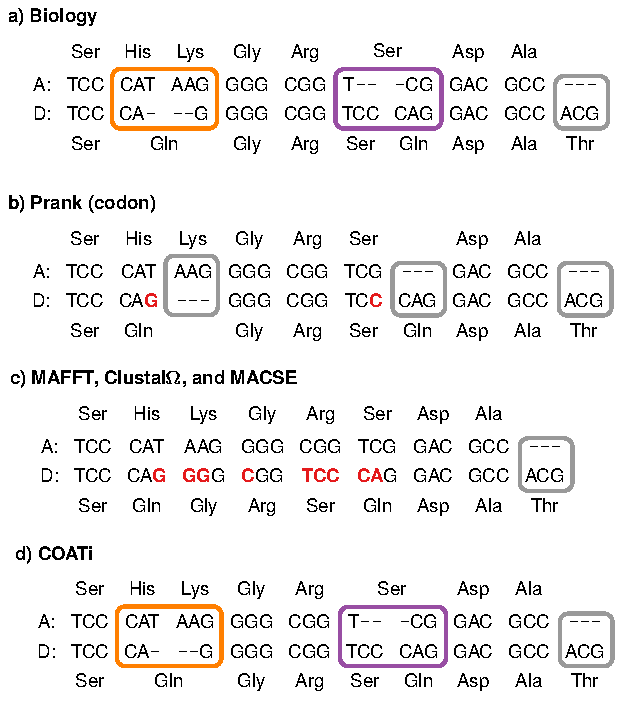
\includegraphics[scale=1]{fig-aln.pdf}
    \par
    \caption[Suboptimal alignments and indel phases]{
        Standard algorithms produce suboptimal alignments.
        (a) shows the true alignment of an ancestor sequence (A) and a descendant sequence (D).
        (b), (c), and (d) are the results of different aligners.
        Nucleotide mismatches are highlighted in red. Phase 0, phase 1, and phase 2 indels are shown in gray, purple, and orange, respectively.
        Additionally, the orange indel is type II (an amino-acid indel plus an amino-acid change) while the purple indel is type I (an amino-acid indel only).
        COATi is the only aligner able to retrieve the biological alignment in this example.
        }
    \label{fig:aln}
\end{figure}

Genome quality impacts conclusions drawn from comparative genomic studies, and uncorrected errors in the alignment stage can lead to erroneous results in comparative and functional genomic studies \citep{estimates_schneider_2009,effect_fletcher_2010,hubisz2011error}.
Genomes for model organisms often get refined over many iterations and achieve high quality with meticulously curated protein coding sequences.
In contrast, genomes for non-model organisms might only receive partial curation and typically have lower-quality sequences and annotations.
These genomes often lack the amount of sequencing data needed to fix artifacts, including missing exons, erroneous mutations, and indels \citep{jackman2018tigmint}.
%
When comparative and functional genomics studies include data from non-model organisms, care must be taken to identify and manage such artifacts; however,
current alignment methods are ill-equipped to handle common artifacts in genomic data, requiring costly curation practices that discard significant amounts of information.
To address this problem, I developed COATi, short for COdon-aware Alignment Transducer, a pairwise statistical aligner that incorporates codon substitution models and is robust to artifacts present in modern genomic data.

\section{Materials}

\subsection{Finite State Transducers}

Statistical alignment is typically performed using pairwise hidden Markov models (pair-HMMs), which have the ability to rigorously model molecular sequence evolution \citep{bradley2007transducers}.
Pair-HMMs are computational machines with probabilities for emitting symbols from the states to two output tapes and probabilities for the transitions between the states (arcs). Each tape represents a sequence and a path through these computational machines is a possible pairwise alignment. Pair-HMMs contain a finite number of states, typically labeled match (M), insert (I), and delete (D). The emission probability distribution of M usually follows a substitution model for emitting an aligned pair or symbols ($s_i,v_j$) from sequences $s$ and $v$. States I and D have distributions for emitting symbols against a gap (-). In addition, arcs in pair-HMMs have transition probabilities. Figure \ref{fig:hmm} illustrates a common pair-HMM architecture, with affine gap scoring. Conceptually, these machines generate two sequences, $s$ and $v$, from an unknown ancestor and can calculate the probability that two sequences are related, represented by $P(s, v)$ \citep{yoon_2009_hmm}.

\clearpage

\begin{figure}[!ht]
    \centering
    \resizebox{0.8\textwidth}{!}{% % !TEX program=lualatex
\definecolor{colorR}{RGB}{228,26,28}    % RED
\definecolor{colorB}{RGB}{55,126,184}   % BLUE
\definecolor{colorG}{RGB}{77,175,74}    % GREEN
\definecolor{colorP}{RGB}{152,78,163}   % PURPLE
\definecolor{colorO}{RGB}{255,127,0}    % ORANGE
\definecolor{colorY}{RGB}{255,255,51}   % YELLOW
\definecolor{colorBn}{RGB}{166,86,40}   % BROWN
\definecolor{colorPk}{RGB}{247,129,191} % PINK
\definecolor{colorGy}{RGB}{153,153,153} % GRAY

\tikzstyle{line}=[draw, -stealth', very thick]
\tikzstyle{block}=[circle,fill=colorB!50,on grid,font=\large]
\tikzstyle{lab}=[]
\tikzstyle{w}=[lab,midway]
\tikzstyle{e}=[lab,midway,auto=false,fill=colorP!50,font=\scriptsize]

\begin{tikzpicture}[node distance=40mm, auto,
	dottedline/.style = {ultra thick, loosely dotted,shorten >=1mm, shorten <=1mm}]
%%% Legend

%%% Indel FST
\node[block,align=center] (M) {\textbf{M}\\$s_i,v_j$};
\node[block,above right=25mm and 25mm of M,align=center] (I) {\textbf{I}\\$-,v_j$};
\node[block,below right=25mm and 25mm of M,align=center] (D) {\textbf{D}\\$s_i,-$};

\draw[line] (M) to[out=90,in=180] node[w,left=5mm] {$\delta$} (I);
\draw[line] (I) to[out=270,in=10] node[w,right=2mm] {$1-\varepsilon$} (M);

\draw[line] (M) to[out=270,in=180] node[w,left=5mm] {$\delta$} (D);
\draw[line] (D) to[out=90,in=350] node[w,right=2mm] {$1-\varepsilon$} (M);

\draw[line] (M.135) arc (45:302:8mm) node[w,left] {$1-2\delta$};
\draw[line] (I.45) arc (135:-120:8mm) node[w,right] {$\varepsilon$};
\draw[line] (D.45) arc (135:-122:8mm) node[w,right] {$\varepsilon$};

\node[font=\footnotesize,text width=50mm,below=4cm of M] (sequences) {
\begin{tabular}{r@{\,: }l}
\multicolumn{2}{l}{\textbf{Sequences}}\\
    \hline
	% X & input nucleotides\\
	% Y & intermediate nucleotides\\
	$s,v$ & sequences\\
	% \O & nothing/empty sequence\\
\end{tabular}
};

\node[font=\footnotesize,right=0.5cm of sequences,text width=50mm] {
\begin{tabular}{r@{\,: }l}
\multicolumn{2}{l}{\textbf{Parameters}}\\
\hline
	$\delta$ & gap open weight\\
	$\varepsilon$ & gap extension weight\\
\end{tabular}
};


\end{tikzpicture}

}
    \caption[Pair-HMM]{Example of a typical pair hidden Markov model (pair-HMM) used in statistical pairwise sequence alignment. Sequences $s$ and $v$ are aligned using an affine gap scoring model and a substitution model (unspecified). The arcs are weighted with gap opening parameter $\delta$ and gap extension $\varepsilon$, therefore defining no gap opening weight as $1-\delta$ and gap closing as $1-\varepsilon$.}
    \label{fig:hmm}
\end{figure}

A limitation of pair-HMMs is that they only model the evolution of two related sequences from an unknown ancestor.
Finite-state transducers (FSTs) have similar benefits to pair-HMMs with the additional feature that \DIFaddbegin \DIFadd{they }\DIFaddend can model the generation of a descendant sequence given an ancestral one.
FSTs, similar to pair-HMMS, are computational machines with a symbol alphabet, a set of states, and weighted arcs defining the transition probabilities between states. However, FSTs consume symbols from an input and emit symbols to an output tape ($a:b$), as opposed to having two output tapes ($a,b$). Properly weighted, an FST can calculate the probability that a descendant sequence, $v$, evolved from an ancestral sequence, $s$, represented by $P(v | s)$.

Furthermore, well-established algorithms for combining FSTs in different ways, including concatenation, composition, intersection, union, or reversal, allow the design of complex models by combining simpler FSTs \citep{bradley2007transducers,silvestre2021machine}.
Specifically, composition is a powerful and versatile algorithm for comparative sequence analysis, consisting of sending the output of one FST into the input of a second FST.
Composition allows combining two or more FSTs to create a new, more complex transducer. Figure \ref{fig:transcription} illustrates how DNA transcription for a codon can be achieved by composing a complimenting FST with a transducer that replaces thymines with uracil, where the three nucleotides are read and complimented in \ref{fig:transcription}-a, which are then used as the input of \ref{fig:transcription}-b, resulting in the transcription of the codon (Fig.~\ref{fig:transcription}-c). COATi uses composition to derive a statistical alignment model from the combination of smaller FSTs, each representing a specific process.

\begin{figure}[!ht]
    \centering
    \hspace*{-3.5em}\DIFdelbeginFL %DIFDELCMD < \resizebox{1.05\textwidth}{!}{\definecolor{colorR}{RGB}{228,26,28}    % RED
%DIFDELCMD < \definecolor{colorB}{RGB}{55,126,184}   % BLUE
%DIFDELCMD < \definecolor{colorG}{RGB}{77,175,74}    % GREEN
%DIFDELCMD < \definecolor{colorP}{RGB}{152,78,163}   % PURPLE
%DIFDELCMD < \definecolor{colorO}{RGB}{255,127,0}    % ORANGE
%DIFDELCMD < \definecolor{colorY}{RGB}{255,255,51}   % YELLOW
%DIFDELCMD < \definecolor{colorBn}{RGB}{166,86,40}   % BROWN
%DIFDELCMD < \definecolor{colorPk}{RGB}{247,129,191} % PINK
%DIFDELCMD < \definecolor{colorGy}{RGB}{153,153,153} % GRAY
%DIFDELCMD < 

%DIFDELCMD < \tikzstyle{line}=[draw, -stealth', very thick]
%DIFDELCMD < \tikzstyle{block}=[circle,fill=colorB!50,on grid]
%DIFDELCMD < \tikzstyle{lab}=[]
%DIFDELCMD < \tikzstyle{w}=[lab,midway]
%DIFDELCMD < \tikzstyle{e}=[lab,midway,below=-4mm,auto=false,font=\scriptsize]
%DIFDELCMD < 

%DIFDELCMD < % \begin{document}
%DIFDELCMD < % \begin{tikzpicture}[node distance=25mm, auto]
%DIFDELCMD < \begin{tikzpicture}[node distance=25mm, auto,
%DIFDELCMD < 	dottedline/.style = {ultra thick, loosely dotted,shorten >=1mm, shorten <=1mm}]
%DIFDELCMD < 

%DIFDELCMD < % complimenting FST
%DIFDELCMD < \node (titlea) {\textbf{a) DNA Complimenting}};
%DIFDELCMD < 

%DIFDELCMD < \node[block,below left=1.5cm and -10mm of titlea.west,fill=colorG!50] (start1) {start};
%DIFDELCMD < \node[block,right=15mm of start1,minimum size=20pt] (cod0) {};
%DIFDELCMD < \node[block,right=20mm of cod0,minimum size=20pt] (cod1) {};
%DIFDELCMD < \node[block,right=20mm of cod1,minimum size=20pt] (cod2) {};
%DIFDELCMD < \node[block,right=20mm of cod2,minimum size=20pt] (cod3) {};
%DIFDELCMD < \node[block,fill=colorR!50,right=15mm of cod3] (end1) {end};
%DIFDELCMD < 

%DIFDELCMD < \draw[line] (start1) -- (cod0);
%DIFDELCMD < \draw[line] (cod3) -- (end1);
%DIFDELCMD < 

%DIFDELCMD < \draw[line] (cod0) to[bend right=-60] node[e] {A:T} (cod1);
%DIFDELCMD < \draw[line] (cod0) to[bend right=-25] node[e] {C:G} (cod1);
%DIFDELCMD < \draw[line] (cod0) to[bend right=25] node[e,below=-4.5mm] {G:C} (cod1);
%DIFDELCMD < \draw[line] (cod0) to[bend right=60] node[e] {T:A} (cod1);
%DIFDELCMD < 

%DIFDELCMD < \draw[line] (cod1) to[bend right=-60] node[e] {A:T} (cod2);
%DIFDELCMD < \draw[line] (cod1) to[bend right=-25] node[e] {C:G} (cod2);
%DIFDELCMD < \draw[line] (cod1) to[bend right=25] node[e,below=-4.5mm] {G:C} (cod2);
%DIFDELCMD < \draw[line] (cod1) to[bend right=60] node[e] {T:A} (cod2);
%DIFDELCMD < 

%DIFDELCMD < \draw[line] (cod2) to[bend right=-60] node[e] {A:T} (cod3);
%DIFDELCMD < \draw[line] (cod2) to[bend right=-25] node[e] {C:G} (cod3);
%DIFDELCMD < \draw[line] (cod2) to[bend right=25] node[e,below=-4.5mm] {G:C} (cod3);
%DIFDELCMD < \draw[line] (cod2) to[bend right=60] node[e] {T:A} (cod3);
%DIFDELCMD < 

%DIFDELCMD < % T->U
%DIFDELCMD < \node[right=6cm of titlea] (titleb) {\textbf{b) Replacing thymine with uracil}};
%DIFDELCMD < 

%DIFDELCMD < \node[block,below right=1.5cm and 12mm of titleb.west,fill=colorG!50] (start2) {start};
%DIFDELCMD < \node[block,right=20mm of start2,minimum size=30pt] (cod4) {};
%DIFDELCMD < \node[block,fill=colorR!50,right=20mm of cod4] (end2) {end};
%DIFDELCMD < 

%DIFDELCMD < \draw[line] (start2) -- (cod4);
%DIFDELCMD < \draw[line] (cod4) -- (end2);
%DIFDELCMD < 

%DIFDELCMD < \draw[line] (cod4) to[out=165,in=105,min distance=2mm,looseness=5] node[e,below left=0.5mm and -6mm] {A:A} (cod4);
%DIFDELCMD < \draw[line] (cod4) to[out=85,in=15,min distance=2mm,looseness=5] node[e,below left=0.5mm and -1mm] {C:C} (cod4);
%DIFDELCMD < \draw[line] (cod4) to[out=-15,in=285,min distance=2mm,looseness=5] node[e,above left=0.5mm and -1mm] {G:G} (cod4);
%DIFDELCMD < \draw[line] (cod4) to[out=255,in=195,min distance=2mm,looseness=5] node[e,above left=0.5mm and -6mm] {T:U} (cod4);
%DIFDELCMD < 

%DIFDELCMD < % transcription FST
%DIFDELCMD < \node[below right=35mm and 25mm of titlea.west] (titlec) {\textbf{c) DNA Transcription}};
%DIFDELCMD < 

%DIFDELCMD < \node[block,below right=1.5cm and 1cm of titlec.west,fill=colorG!50] (start3) {start};
%DIFDELCMD < \node[block,right=15mm of start3,minimum size=20pt] (cod5) {};
%DIFDELCMD < \node[block,right=20mm of cod5,minimum size=20pt] (cod6) {};
%DIFDELCMD < \node[block,right=20mm of cod6,minimum size=20pt] (cod7) {};
%DIFDELCMD < \node[block,right=20mm of cod7,minimum size=20pt] (cod8) {};
%DIFDELCMD < \node[block,fill=colorR!50,right=15mm of cod8] (end3) {end};
%DIFDELCMD < 

%DIFDELCMD < \draw[line] (start3) -- (cod5);
%DIFDELCMD < \draw[line] (cod8) -- (end3);
%DIFDELCMD < 

%DIFDELCMD < \draw[line] (cod5) to[bend right=-60] node[e] {A:U} (cod6);
%DIFDELCMD < \draw[line] (cod5) to[bend right=-25] node[e] {C:G} (cod6);
%DIFDELCMD < \draw[line] (cod5) to[bend right=25] node[e,below=-4.5mm] {G:C} (cod6);
%DIFDELCMD < \draw[line] (cod5) to[bend right=60] node[e] {T:A} (cod6);
%DIFDELCMD < 

%DIFDELCMD < \draw[line] (cod6) to[bend right=-60] node[e] {A:U} (cod7);
%DIFDELCMD < \draw[line] (cod6) to[bend right=-25] node[e] {C:G} (cod7);
%DIFDELCMD < \draw[line] (cod6) to[bend right=25] node[e,below=-4.5mm] {G:C} (cod7);
%DIFDELCMD < \draw[line] (cod6) to[bend right=60] node[e] {T:A} (cod7);
%DIFDELCMD < 

%DIFDELCMD < \draw[line] (cod7) to[bend right=-60] node[e] {A:U} (cod8);
%DIFDELCMD < \draw[line] (cod7) to[bend right=-25] node[e] {C:G} (cod8);
%DIFDELCMD < \draw[line] (cod7) to[bend right=25] node[e,below=-4.5mm] {G:C} (cod8);
%DIFDELCMD < \draw[line] (cod7) to[bend right=60] node[e] {T:A} (cod8);
%DIFDELCMD < 

%DIFDELCMD < \end{tikzpicture}}
%DIFDELCMD <     %%%
\DIFdelendFL \DIFaddbeginFL \resizebox{1.05\textwidth}{!}{\definecolor{colorR}{RGB}{228,26,28}    % RED
\definecolor{colorB}{RGB}{55,126,184}   % BLUE
\definecolor{colorG}{RGB}{77,175,74}    % GREEN
\definecolor{colorP}{RGB}{152,78,163}   % PURPLE
\definecolor{colorO}{RGB}{255,127,0}    % ORANGE
\definecolor{colorY}{RGB}{255,255,51}   % YELLOW
\definecolor{colorBn}{RGB}{166,86,40}   % BROWN
\definecolor{colorPk}{RGB}{247,129,191} % PINK
\definecolor{colorGy}{RGB}{153,153,153} % GRAY

\tikzstyle{line}=[draw, -stealth', very thick]
\tikzstyle{block}=[circle,fill=colorB!50,on grid]
\tikzstyle{lab}=[]
\tikzstyle{w}=[lab,midway]
\tikzstyle{e}=[lab,midway,below=-4mm,auto=false,font=\scriptsize]

% \begin{document}
% \begin{tikzpicture}[node distance=25mm, auto]
\begin{tikzpicture}[node distance=25mm, auto,
	dottedline/.style = {ultra thick, loosely dotted,shorten >=1mm, shorten <=1mm}]

% complimenting FST
\node (titlea) {\textbf{a) DNA Complement}};

\node[block,below left=1.5cm and -10mm of titlea.west,fill=colorG!50] (start1) {start};
\node[block,right=15mm of start1,minimum size=20pt] (cod0) {};
\node[block,right=20mm of cod0,minimum size=20pt] (cod1) {};
\node[block,right=20mm of cod1,minimum size=20pt] (cod2) {};
\node[block,right=20mm of cod2,minimum size=20pt] (cod3) {};
\node[block,fill=colorR!50,right=15mm of cod3] (end1) {end};

\draw[line] (start1) -- (cod0);
\draw[line] (cod3) -- (end1);

\draw[line] (cod0) to[bend right=-60] node[e] {A:T} (cod1);
\draw[line] (cod0) to[bend right=-25] node[e] {C:G} (cod1);
\draw[line] (cod0) to[bend right=25] node[e,below=-4.5mm] {G:C} (cod1);
\draw[line] (cod0) to[bend right=60] node[e] {T:A} (cod1);

\draw[line] (cod1) to[bend right=-60] node[e] {A:T} (cod2);
\draw[line] (cod1) to[bend right=-25] node[e] {C:G} (cod2);
\draw[line] (cod1) to[bend right=25] node[e,below=-4.5mm] {G:C} (cod2);
\draw[line] (cod1) to[bend right=60] node[e] {T:A} (cod2);

\draw[line] (cod2) to[bend right=-60] node[e] {A:T} (cod3);
\draw[line] (cod2) to[bend right=-25] node[e] {C:G} (cod3);
\draw[line] (cod2) to[bend right=25] node[e,below=-4.5mm] {G:C} (cod3);
\draw[line] (cod2) to[bend right=60] node[e] {T:A} (cod3);

% T->U
\node[right=6cm of titlea] (titleb) {\textbf{b) Replacing thymine with uracil}};

\node[block,below right=1.5cm and 12mm of titleb.west,fill=colorG!50] (start2) {start};
\node[block,right=20mm of start2,minimum size=30pt] (cod4) {};
\node[block,fill=colorR!50,right=20mm of cod4] (end2) {end};

\draw[line] (start2) -- (cod4);
\draw[line] (cod4) -- (end2);

\draw[line] (cod4) to[out=165,in=105,min distance=2mm,looseness=5] node[e,below left=0.5mm and -6mm] {A:A} (cod4);
\draw[line] (cod4) to[out=85,in=15,min distance=2mm,looseness=5] node[e,below left=0.5mm and -1mm] {C:C} (cod4);
\draw[line] (cod4) to[out=-15,in=285,min distance=2mm,looseness=5] node[e,above left=0.5mm and -1mm] {G:G} (cod4);
\draw[line] (cod4) to[out=255,in=195,min distance=2mm,looseness=5] node[e,above left=0.5mm and -6mm] {T:U} (cod4);

% transcription FST
\node[below right=35mm and 25mm of titlea.west] (titlec) {\textbf{c) DNA Transcription}};

\node[block,below right=1.5cm and 1cm of titlec.west,fill=colorG!50] (start3) {start};
\node[block,right=15mm of start3,minimum size=20pt] (cod5) {};
\node[block,right=20mm of cod5,minimum size=20pt] (cod6) {};
\node[block,right=20mm of cod6,minimum size=20pt] (cod7) {};
\node[block,right=20mm of cod7,minimum size=20pt] (cod8) {};
\node[block,fill=colorR!50,right=15mm of cod8] (end3) {end};

\draw[line] (start3) -- (cod5);
\draw[line] (cod8) -- (end3);

\draw[line] (cod5) to[bend right=-60] node[e] {A:U} (cod6);
\draw[line] (cod5) to[bend right=-25] node[e] {C:G} (cod6);
\draw[line] (cod5) to[bend right=25] node[e,below=-4.5mm] {G:C} (cod6);
\draw[line] (cod5) to[bend right=60] node[e] {T:A} (cod6);

\draw[line] (cod6) to[bend right=-60] node[e] {A:U} (cod7);
\draw[line] (cod6) to[bend right=-25] node[e] {C:G} (cod7);
\draw[line] (cod6) to[bend right=25] node[e,below=-4.5mm] {G:C} (cod7);
\draw[line] (cod6) to[bend right=60] node[e] {T:A} (cod7);

\draw[line] (cod7) to[bend right=-60] node[e] {A:U} (cod8);
\draw[line] (cod7) to[bend right=-25] node[e] {C:G} (cod8);
\draw[line] (cod7) to[bend right=25] node[e,below=-4.5mm] {G:C} (cod8);
\draw[line] (cod7) to[bend right=60] node[e] {T:A} (cod8);

\end{tikzpicture}}
    \DIFaddendFL \caption[DNA Transcription via FST Composition]{DNA transcription via FST composition. The composition of (a) a codon complimenting FST and (b) an FST that replaces T with U generates (c) an FST that implements codon transcription ($a~\circ$~b = c).}
    \label{fig:transcription}
\end{figure}

%DIF <  \begin{figure}[!ht]
%DIF <      \centering
%DIF <      \begin{subfigure}[c]{0.6\textwidth}
%DIF <          \centering
%DIF <          \includegraphics[scale=0.5,angle=-90]{chapter2/figures/complimenting.pdf}
%DIF <          \caption{DNA complimenting.}
%DIF <       \end{subfigure}
%DIF <      \begin{subfigure}[c]{0.3\textwidth}
%DIF <          \centering
%DIF <          \vspace*{-3em}\includegraphics[scale=0.6,angle=-90]{chapter2/figures/t2u-2.pdf}
%DIF <          \caption{Replacing thymine with uracil.}
%DIF <       \end{subfigure}
%DIF <      \begin{subfigure}[c]{0.8\textwidth}
%DIF <          \centering
%DIF <          \vspace*{-1em}\includegraphics[scale=0.6,angle=-90]{chapter2/figures/transcripting.pdf}
%DIF <          \caption{DNA transcription.}
%DIF <       \end{subfigure}
%DIF <      \caption[DNA Transcription via FST Composition]{DNA transcription via FST composition. The composition of (a) a codon complimenting FST and (b) an FST that replaces T with U generates (c) an FST that implements codon transcription ($a~\circ$~b = c). Double-circled states are the end states. Figures and composition are generated using the openFST library \citep{allauzen2007openfst}.}
%DIF <      \label{fig:transcription}
%DIF <  \end{figure}
\DIFdelbegin %DIFDELCMD < 

%DIFDELCMD < %%%
\DIFdelend \subsection{Evolution FST}

COATi implements the pairwise alignment of a potentially lower-quality sequence against a high-quality sequence as a path through the Evolution FST (Fig.~\ref{fig:evolution-fst}) \citep[c.f.][]{holmes2001evolutionary}.
Here, COATi treats the high-quality (reference) sequence as the ``ancestor'' and the potentially lower-quality sequence as the ``descendant''. The assumption is that the reference sequence is in-phase, which is used to help preserve the reading frame and safeguard against possible frameshifts in the ``descendant''. Therefore, the high-quality sequence must not contain incomplete codons (the number of nucleotides is multiple of three) and be free of any ambiguous nucleotides or early stop codons. In contrast, the potentially lower-quality sequence has no such restrictions and can be of any length, contain early stop codons---treated as artifacts---, and include ambiguous codons.

The Evolution FST is the result of composing a substitution FST that encodes a codon model (Fig.\ \ref{fig:evolution-fst}-a), an indel FST that models insertions and deletions, including frameshifts (Fig.\ \ref{fig:evolution-fst}-b), and a base calling error FST that models incorrectly sequenced bases (Fig~\ref{fig:evolution-fst}-b).
A key innovation of this FST, with respect to others, is the combination of a codon substitution model with a nucleotide-based geometric indel model that allows gaps to occur at any position.

Composing both sequences with the Evolution FST results in the transducer of all possible alignments.
Any path through this FST represents a pairwise alignment, while the shortest path (by weight) corresponds to the best alignment.
All FST operations in COATi, including model development, composition, search for the shortest path, and other optimization algorithms, are performed using the C\texttt{++} openFST library \citep{allauzen2007openfst}.
However, the Evolution FST has a large state space to keep track of codon substitution rates when codons might be interspersed with indel events. This additional state space increases the computational complexity of the alignment algorithm.

\begin{figure}[!ht]
\centering
\hspace*{-4em}\resizebox{0.95\textwidth}{!}{\definecolor{colorR}{RGB}{228,26,28}    % RED
\definecolor{colorB}{RGB}{55,126,184}   % BLUE
\definecolor{colorG}{RGB}{77,175,74}    % GREEN
\definecolor{colorP}{RGB}{152,78,163}   % PURPLE
\definecolor{colorO}{RGB}{255,127,0}    % ORANGE
\definecolor{colorY}{RGB}{255,255,51}   % YELLOW
\definecolor{colorBn}{RGB}{166,86,40}   % BROWN
\definecolor{colorPk}{RGB}{247,129,191} % PINK
\definecolor{colorGy}{RGB}{153,153,153} % GRAY

\tikzstyle{line}=[draw, -stealth', very thick]
\tikzstyle{block}=[circle,fill=colorB!50,on grid]
\tikzstyle{lab}=[]
\tikzstyle{w}=[lab,midway]
\tikzstyle{e}=[lab,midway,above=0.2mm,auto=false,font=\scriptsize]

% \begin{document}
% \begin{tikzpicture}[node distance=25mm, auto]
\begin{tikzpicture}[node distance=25mm, auto,
	dottedline/.style = {ultra thick, loosely dotted,shorten >=1mm, shorten <=1mm}]
%%% MG94 marginal substitution FST
\node (titlea) {\textbf{a) Substitution}};

\node[block,below=1.5cm of titlea,fill=colorG!50] (start_sub) {start};
\node[block,right=15mm of start_sub] (S_sub) {M};
\node[block,right=75mm of S_sub] (M_sub) {S};
\node[block,fill=colorR!50,right=15mm of M_sub] (end_sub) {end};

% AAA->AAA
\node[block,above right=12mm and 20mm of S_sub,minimum size=15pt] (s2) {};
\node[block,above right=3mm and 20mm of s2,minimum size=15pt] (s1) {};
% % AAA->AAC
\node[block,above right=4mm and 20mm of S_sub,minimum size=15pt] (s4) {};
\node[block,below right=-1mm and 20mm of s4,minimum size=15pt] (s3) {};
% TTT->TTT
\node[block,below right=6mm and 20mm of S_sub,minimum size=15pt] (s122) {};
\node[block,below right=3mm and 20mm of s122,minimum size=15pt] (s121) {};

\draw[line] (start_sub) -- (S_sub);
\draw[line] (S_sub) to[bend right=40] (M_sub);
\draw[line] (M_sub) -- (end_sub);

% AAA->AAA
% \draw[line] (M_sub) to[bend right=15] node[w,pos=0.7,above right=3mm and 1mm,font=\scriptsize,rotate=-20] {$P(AAA|AAA)$} (s1);
\draw[line] (M_sub) to[bend right=15] node[e,pos=0.4,rotate=-20] {A:A/$P(AAA|AAA)$} (s1);
\draw[line] (s1) to[bend right=15] node[e,pos=0.5] {A:A} (s2);
\draw[line] (s2) to[bend right=15] node[e,pos=0.5] {A:A} (S_sub);

% % AAA->AAC
\draw[line] (M_sub) to[bend right=5] node[e,pos=0.5,rotate=-8,below=-5mm] {A:A/$P(AAC|AAA)$} (s3);
\draw[line] (s3) to[bend right=8] node[e,pos=0.5] {A:A} (s4);
\draw[line] (s4) to[bend right=8] node[e,pos=0.5] {A:C} (S_sub);

\node[below=9mm of s1,font=\Huge] {$\vdots$};
\node[below=5mm of s2,font=\Huge] {$\vdots$};

% TTT->TTT
% \draw[line] (M_sub) to[bend right=-5] node[w,pos=0.5,above right=1mm and -11mm, rotate=5,font=\scriptsize] {$P(TTT|TTT)$} (s121);
\draw[line] (M_sub) to[bend right=-5] node[e,pos=0.5,rotate=9] {T:T/$P(TTT|TTT)$} (s121);
\draw[line] (s121) to[bend right=-5] node[e,pos=0.5] {T:T} (s122);
\draw[line] (s122) to[bend right=-5] node[e,pos=0.4] {T:T} (S_sub);

%%% Indel FST
\node[below left=3cm and -14mm of titlea.east] (titleb) {\textbf{b) Insertion-Deletion}};

\node[block,below right=1.5cm and 1cm of titleb,fill=colorG!50] (start1) {start};
\node[block,below=15mm of start1] (S1) {M};
\node[block,below=of S1] (I1) {U};
\node[block,right=of I1] (U1) {I};
\node[block,above=of U1] (W1) {W};
\node[block,above=20mm of W1] (D1) {V};
\node[block,right=of D1] (V1) {D};
\node[block,right=of W1] (M1) {S};
\node[block,fill=colorR!50,right=20mm of M1] (end1) {end};

\draw (D1) +(0mm,-20mm) coordinate (C1);
\draw (D1) +(50mm,-10mm) coordinate (C2);

\draw[line] (start1) -- (S1);
\draw[line] (S1) -- node[w] {$g$} (I1);
\draw[line] (S1) -- node[w] {$1-g$} (W1);
\draw[line] (U1) to[out=150,in=30]  node[w,above] {$e$} (I1);
\draw[line] (U1) -- node[w,pos=0.1,right] {$1-e$} (W1);
\draw[line] (W1) -- node[w] {$g$} (D1);
\draw[line] (W1) -- node[w] {$1-g$} (M1);
\draw[line] (M1) -- node[w] {} (end1);
\draw[line] (V1) to[out=150,in=30] node[w,above] {$e$} (D1);
\draw[line] (V1) -- node[w,swap] {$1-e$} (M1);


\draw[line] (I1) to[bend right=20] (U1);
\draw[line] (I1) to[bend right=25] (U1);
\draw[line] (I1) to[bend right=30] (U1);
\draw[line] (I1) to[bend right=35] (U1);
\draw[line] (I1) to[bend right=40] node[e,fill=white] {\O:Z/$\grande{\pi}_{\text{Z}}$} (U1);

\draw[line] (D1) to[bend right=20] (V1);
\draw[line] (D1) to[bend right=25] (V1);
\draw[line] (D1) to[bend right=35] (V1);
\draw[line] (D1) to[bend right=30] (V1);
\draw[line] (D1) to[bend right=40] node[e,fill=white] {Y:\O} (V1);

\draw[line] (M1) to[bend left=39] (S1);
\draw[line] (M1) to[bend left=42] (S1);
\draw[line] (M1) to[bend left=48] (S1);
\draw[line] (M1) to[bend left=51] (S1);

\draw[line] (M1) to[bend left=45] node[e,pos=0.30,fill=white] {Y:Z} (S1);

%%%% Base calling error FST
\node[below left=10cm and -16mm of titlea.east] (titlec) {\textbf{c) Base Calling Error}};

\node[block,below=1.5cm of titlec,fill=colorG!50] (start_bce) {start};
\node[block,right=15mm of start_bce] (S_bce) {M};
\node[block,right=60mm of S_bce] (M_bce) {S};
\node[block,fill=colorR!50,right=15mm of M_bce] (end_bce) {end};

\draw[line] (start_bce) -- (S_bce);
\draw[line] (M_bce) -- (end_bce);

% \draw[line] (M_bce) to[bend right=25] node[w,below=1mm,pos=0.66] {$\varepsilon$} (S_bce);
\draw[line] (M_bce) to[bend right=25] node[e] {Y$_\text{i}$:Y$_\text{j}$/$\grande{\varepsilon}$} (S_bce);
% \draw[line] (M_bce) to node[w,below=0.2mm,pos=0.66] {$1 - 3 \cdot \varepsilon$} (S_bce);
\draw[line] (M_bce) to node[e] {Y$_\text{i}$:Y$_\text{i}$/$1-3\cdot \grande{\varepsilon}$} (S_bce);
\draw[line] (M_bce) to[bend right=-25] (S_bce);
\draw[line] (M_bce) to[bend right=-25] node[e] {Y$_\text{i}$:N} (S_bce);

\draw[line] (S_bce) to[bend left=-60] (M_bce);

%%% Legend

% \node[below left=2cm and 1.5cm of start_bce,text width=50mm,anchor=north west] (sequences) {
\node[above right=2mm and 5.5cm of titleb,text width=50mm,anchor=north west] (sequences) {
\begin{tabular}{r@{\,: }l}
\multicolumn{2}{l}{\textbf{Sequences}}\\
    \hline
	X & input nucleotides\\
	Y & intermediate nucleotides\\
	Z & output nucleotides\\
	\O & nothing/empty sequence\\
        % Y$_i$:Y$_i$ & matches\\
        % Y$_i$:Y$_j$ & mismatches\\
 % 	$i \rightarrow i$ & matching input to intermediate base\\
	% $i \rightarrow j$ & mismatching input to intermediate base\\
	% $i \rightarrow N$ & input to intermediate ambiguous base N\\
\end{tabular}
};

% \node[above right=-2.85cm and 5mm of sequences,text width=50mm] {
\node[below=1.5cm of sequences,text width=50mm] {
\begin{tabular}{r@{\,: }l}
\multicolumn{2}{l}{\textbf{Parameters}}\\
\hline
	$g$ & gap open weight\\
	$e$ & gap extension weight\\
	$\pi$ & nucleotide stationary freq.\\
        $\varepsilon$ & base calling error weight\\
\end{tabular}
};

\end{tikzpicture}
% \end{document}
}
% \hspace*{-3.5em}\scalebox{0.75}{\definecolor{colorR}{RGB}{228,26,28}    % RED
\definecolor{colorB}{RGB}{55,126,184}   % BLUE
\definecolor{colorG}{RGB}{77,175,74}    % GREEN
\definecolor{colorP}{RGB}{152,78,163}   % PURPLE
\definecolor{colorO}{RGB}{255,127,0}    % ORANGE
\definecolor{colorY}{RGB}{255,255,51}   % YELLOW
\definecolor{colorBn}{RGB}{166,86,40}   % BROWN
\definecolor{colorPk}{RGB}{247,129,191} % PINK
\definecolor{colorGy}{RGB}{153,153,153} % GRAY

\tikzstyle{line}=[draw, -stealth', very thick]
\tikzstyle{block}=[circle,fill=colorB!50,on grid]
\tikzstyle{lab}=[]
\tikzstyle{w}=[lab,midway]
\tikzstyle{e}=[lab,midway,above=0.2mm,auto=false,font=\scriptsize]

% \begin{document}
% \begin{tikzpicture}[node distance=25mm, auto]
\begin{tikzpicture}[node distance=25mm, auto,
	dottedline/.style = {ultra thick, loosely dotted,shorten >=1mm, shorten <=1mm}]
%%% MG94 marginal substitution FST
\node (titlea) {\textbf{a) Substitution}};

\node[block,below=1.5cm of titlea,fill=colorG!50] (start_sub) {start};
\node[block,right=15mm of start_sub] (S_sub) {M};
\node[block,right=75mm of S_sub] (M_sub) {S};
\node[block,fill=colorR!50,right=15mm of M_sub] (end_sub) {end};

% AAA->AAA
\node[block,above right=12mm and 20mm of S_sub,minimum size=15pt] (s2) {};
\node[block,above right=3mm and 20mm of s2,minimum size=15pt] (s1) {};
% % AAA->AAC
\node[block,above right=4mm and 20mm of S_sub,minimum size=15pt] (s4) {};
\node[block,below right=-1mm and 20mm of s4,minimum size=15pt] (s3) {};
% TTT->TTT
\node[block,below right=6mm and 20mm of S_sub,minimum size=15pt] (s122) {};
\node[block,below right=3mm and 20mm of s122,minimum size=15pt] (s121) {};

\draw[line] (start_sub) -- (S_sub);
\draw[line] (S_sub) to[bend right=40] (M_sub);
\draw[line] (M_sub) -- (end_sub);

% AAA->AAA
% \draw[line] (M_sub) to[bend right=15] node[w,pos=0.7,above right=3mm and 1mm,font=\scriptsize,rotate=-20] {$P(AAA|AAA)$} (s1);
\draw[line] (M_sub) to[bend right=15] node[e,pos=0.4,rotate=-20] {A:A/$P(AAA|AAA)$} (s1);
\draw[line] (s1) to[bend right=15] node[e,pos=0.5] {A:A} (s2);
\draw[line] (s2) to[bend right=15] node[e,pos=0.5] {A:A} (S_sub);

% % AAA->AAC
\draw[line] (M_sub) to[bend right=5] node[e,pos=0.5,rotate=-8,below=-5mm] {A:A/$P(AAC|AAA)$} (s3);
\draw[line] (s3) to[bend right=8] node[e,pos=0.5] {A:A} (s4);
\draw[line] (s4) to[bend right=8] node[e,pos=0.5] {A:C} (S_sub);

\node[below=9mm of s1,font=\Huge] {$\vdots$};
\node[below=5mm of s2,font=\Huge] {$\vdots$};

% TTT->TTT
% \draw[line] (M_sub) to[bend right=-5] node[w,pos=0.5,above right=1mm and -11mm, rotate=5,font=\scriptsize] {$P(TTT|TTT)$} (s121);
\draw[line] (M_sub) to[bend right=-5] node[e,pos=0.5,rotate=9] {T:T/$P(TTT|TTT)$} (s121);
\draw[line] (s121) to[bend right=-5] node[e,pos=0.5] {T:T} (s122);
\draw[line] (s122) to[bend right=-5] node[e,pos=0.4] {T:T} (S_sub);

%%% Indel FST
\node[below left=3cm and -14mm of titlea.east] (titleb) {\textbf{b) Insertion-Deletion}};

\node[block,below right=1.5cm and 1cm of titleb,fill=colorG!50] (start1) {start};
\node[block,below=15mm of start1] (S1) {M};
\node[block,below=of S1] (I1) {U};
\node[block,right=of I1] (U1) {I};
\node[block,above=of U1] (W1) {W};
\node[block,above=20mm of W1] (D1) {V};
\node[block,right=of D1] (V1) {D};
\node[block,right=of W1] (M1) {S};
\node[block,fill=colorR!50,right=20mm of M1] (end1) {end};

\draw (D1) +(0mm,-20mm) coordinate (C1);
\draw (D1) +(50mm,-10mm) coordinate (C2);

\draw[line] (start1) -- (S1);
\draw[line] (S1) -- node[w] {$g$} (I1);
\draw[line] (S1) -- node[w] {$1-g$} (W1);
\draw[line] (U1) to[out=150,in=30]  node[w,above] {$e$} (I1);
\draw[line] (U1) -- node[w,pos=0.1,right] {$1-e$} (W1);
\draw[line] (W1) -- node[w] {$g$} (D1);
\draw[line] (W1) -- node[w] {$1-g$} (M1);
\draw[line] (M1) -- node[w] {} (end1);
\draw[line] (V1) to[out=150,in=30] node[w,above] {$e$} (D1);
\draw[line] (V1) -- node[w,swap] {$1-e$} (M1);


\draw[line] (I1) to[bend right=20] (U1);
\draw[line] (I1) to[bend right=25] (U1);
\draw[line] (I1) to[bend right=30] (U1);
\draw[line] (I1) to[bend right=35] (U1);
\draw[line] (I1) to[bend right=40] node[e,fill=white] {\O:Z/$\grande{\pi}_{\text{Z}}$} (U1);

\draw[line] (D1) to[bend right=20] (V1);
\draw[line] (D1) to[bend right=25] (V1);
\draw[line] (D1) to[bend right=35] (V1);
\draw[line] (D1) to[bend right=30] (V1);
\draw[line] (D1) to[bend right=40] node[e,fill=white] {Y:\O} (V1);

\draw[line] (M1) to[bend left=39] (S1);
\draw[line] (M1) to[bend left=42] (S1);
\draw[line] (M1) to[bend left=48] (S1);
\draw[line] (M1) to[bend left=51] (S1);

\draw[line] (M1) to[bend left=45] node[e,pos=0.30,fill=white] {Y:Z} (S1);

%%%% Base calling error FST
\node[below left=10cm and -16mm of titlea.east] (titlec) {\textbf{c) Base Calling Error}};

\node[block,below=1.5cm of titlec,fill=colorG!50] (start_bce) {start};
\node[block,right=15mm of start_bce] (S_bce) {M};
\node[block,right=60mm of S_bce] (M_bce) {S};
\node[block,fill=colorR!50,right=15mm of M_bce] (end_bce) {end};

\draw[line] (start_bce) -- (S_bce);
\draw[line] (M_bce) -- (end_bce);

% \draw[line] (M_bce) to[bend right=25] node[w,below=1mm,pos=0.66] {$\varepsilon$} (S_bce);
\draw[line] (M_bce) to[bend right=25] node[e] {Y$_\text{i}$:Y$_\text{j}$/$\grande{\varepsilon}$} (S_bce);
% \draw[line] (M_bce) to node[w,below=0.2mm,pos=0.66] {$1 - 3 \cdot \varepsilon$} (S_bce);
\draw[line] (M_bce) to node[e] {Y$_\text{i}$:Y$_\text{i}$/$1-3\cdot \grande{\varepsilon}$} (S_bce);
\draw[line] (M_bce) to[bend right=-25] (S_bce);
\draw[line] (M_bce) to[bend right=-25] node[e] {Y$_\text{i}$:N} (S_bce);

\draw[line] (S_bce) to[bend left=-60] (M_bce);

%%% Legend

% \node[below left=2cm and 1.5cm of start_bce,text width=50mm,anchor=north west] (sequences) {
\node[above right=2mm and 5.5cm of titleb,text width=50mm,anchor=north west] (sequences) {
\begin{tabular}{r@{\,: }l}
\multicolumn{2}{l}{\textbf{Sequences}}\\
    \hline
	X & input nucleotides\\
	Y & intermediate nucleotides\\
	Z & output nucleotides\\
	\O & nothing/empty sequence\\
        % Y$_i$:Y$_i$ & matches\\
        % Y$_i$:Y$_j$ & mismatches\\
 % 	$i \rightarrow i$ & matching input to intermediate base\\
	% $i \rightarrow j$ & mismatching input to intermediate base\\
	% $i \rightarrow N$ & input to intermediate ambiguous base N\\
\end{tabular}
};

% \node[above right=-2.85cm and 5mm of sequences,text width=50mm] {
\node[below=1.5cm of sequences,text width=50mm] {
\begin{tabular}{r@{\,: }l}
\multicolumn{2}{l}{\textbf{Parameters}}\\
\hline
	$g$ & gap open weight\\
	$e$ & gap extension weight\\
	$\pi$ & nucleotide stationary freq.\\
        $\varepsilon$ & base calling error weight\\
\end{tabular}
};

\end{tikzpicture}
% \end{document}
}
% \includegraphics[width=\textwidth]{fig-evolution-fst.pdf}
\par
\caption[Evolution FST]{The Evolution FST is assembled by composing a substitution FST and an indel FST.
Each node represents a state in an FST while arcs display possible transitions between states (and their weights). The arc label format is input symbol : output symbol / weight. Unlabeled arcs have weights of 1, and partially labeled arcs do not consume/emit symbols or have a weight of 1.
(a) The substitution FST encodes a $61 \times 61 $ codon substitution model with 3721 arcs from S to M. These arcs consume three nucleotides from the input tape and emit three nucleotides to the output tape. The weight of each arc is a conditional probability derived from a codon substitution model.
(b) The indel FST allows for insertions (U to I) and deletions (V to D). Insertion arcs are weighted according to the codon model's stationary distribution of nucleotides, and deletion arcs have a weight of 1. Contiguous insertions and deletions are always arranged for insertions to precede deletions to limit equivalent alignments. The base calling error FST (c) is added on top of the indel FST to model sequencing errors. Arcs from S to M generate matches; however, with (c) they can introduce single-nucleotide errors, which allows modeling stop codon artifacts.}
\label{fig:evolution-fst}
\end{figure}

\clearpage

\subsection{Codon Substitution Models} %%%%%%%%%%%%%%%%%%%%%%%%%%%%%%%%%%%%%%%

\subsubsection{Muse and Gaut}

Codon substitution is particularly suitable for modeling protein-coding genes since it accounts for both the likelihood of mutations occurring at the nucleotide level and selective pressure on amino acid substitutions \citep{sullivan2005model}. While codon models are extensively applied to reconstruct phylogenies and study natural selection \citep{delport2009models}, their use in alignment reconstruction is still scarce. COATi is the only aligner that implements the mechanistic Muse and Gaut model (MG94), a codon model designed for coding regions \citep{muse_gaut_1994}. Modeled as a continuous-time Markov process, the instantaneous substitution rate matrix \textit{Q} defines the rate that codon \textit{X} changes to codon \textit{Y} as

%  Q matrix MG94
\begin{align}
Q_{XY} &=  \begin{cases}
    0 & \text{if $X$ and $Y$ differ by more than one nucleotide change}\\
    \grande{\mu}_{X_pY_p} & \text{if $X$ and $Y$ are synonymous}\\
    \omega \cdot \grande{\mu}_{X_pY_p} & \text{if $X$ and $Y$ are nonsynonymous}
\end{cases}\\
Q_{XX} &= -\sum_{Y:Y \neq X} Q_{XY}
\end{align}
where $X$ and $Y$ are non-stop codons defined $X,Y \in \grande{\Sigma}_{codon} - \{\text{TAA, TAG, TGA}\}$, $\omega$ is the strength of selection affecting amino-acid changes, and $X_p$ and $Y_p$ refer to the nucleotides in position \textit{p} in codons \textit{X} and \textit{Y} respectively, defined $X_p, Y_p \in \Sigma_{DNA}$. $\grande{\mu}_{X_pY_p}$ represents the mutation rate that nucleotide $X_p$ is replaced by $Y_p$ defined $\grande{\mu}_{X_pY_p} = \grande{\pi}_{Y_p} \grande{\sigma}_{X_pY_p}, \forall\ X_p \neq Y_p$, where $\grande{\pi}_{Y_p}$ is the equilibrium frequency of nucleotide $Y_p$, and $ \grande{\sigma}_{X_pY_p}$ corresponds to one of the instantaneous substitution parameters (Table \ref{table:gtr-ch2}) of the General Time Reversible nucleotide substitution model \citep{tavare_gtr_1986} (GTR). I use the nucleotide stationary frequencies and GTR parameters inferred from primate data by Yang \citeyear{yang1994estimating} to construct MG94 in COATi.

The GTR model is a well-known and widely-used substitution model that allows \DIFdelbegin \DIFdel{variable }\DIFdelend \DIFaddbegin \DIFadd{different }\DIFaddend instantaneous mutation rates between each of the six nucleotide pairs, with equal forward and reverse rates for any given pair. This property is represented
$\grande{\pi}_{Y_p} \grande{\mu}_{X_pY_p} = \grande{\pi}_{X_p} \grande{\mu}_{Y_pX_p}$
and transfers to the MG94 model,
% $\grande{\pi}_Y Q_{XY} = \grande{\pi}_X Q_{YX}$
making both models time-reversible.

\begin{table}[!ht]
\centering
\begingroup\centering
\begin{tabular}{c||c|c|c|c}
& A & C & G & T\\
\hline\hline
A & $\ast$ & $\grande{\pi}_C \grande{\sigma}_{AC}$ & $\grande{\pi}_G \grande{\sigma}_{AG}$ & $\grande{\pi}_T \sigma_{AT}$\\
C & $\grande{\pi}_A \grande{\sigma}_{CA}$ & $\ast$ & $\grande{\pi}_G \grande{\sigma}_{CG}$ & $\grande{\pi}_T \sigma_{CT}$\\
G & $\grande{\pi}_A \grande{\sigma}_{GA}$ & $\grande{\pi}_C \grande{\sigma}_{GC}$ & $\ast$ & $\grande{\pi}_T \sigma_{GT}$\\
T & $\grande{\pi}_A \grande{\sigma}_{TA}$ & $\grande{\pi}_C \grande{\sigma}_{TC}$ & $\grande{\pi}_G \grande{\sigma}_{TG}$ & $\ast$\\
\end{tabular}
\par\endgroup
 \vspace{2mm}
 \caption[General Time Reversible Model]{Instantaneous nucleotide substitution rates for the General Time Reversible model (GTR). On each row, the parameters represent the probability of a given nucleotide being replaced by another. GTR is the most general and time-reversible nucleotide substitution model, with a different mutation rate parameter for each of the six possible nucleotide combinations. Note that sigma parameters for each of the six possible nucleotide pairs are identical (i.e., $\sigma_{AC} = \sigma_{CA}$, $\sigma_{AG} = \sigma_{GA}$, etc.).}
 \label{table:gtr-ch2}
\end{table}

\subsubsection{Empirical Codon Model}

In addition to the MG94 codon model, COATi incorporates an empirical codon model that can be used with the triplet and marginal alignment procedures. While mechanistic models explicitly account for molecular evolution features and use a defined set of parameters to specify them, empirical models, in contrast, attempt to summarize the substitution patterns inferred from extensive datasets. Although codon substitution models are rare in sequence aligners, the Empirical Codon Model (ECM) is the most common. This model is characterized by incorporating instantaneous doublet and triplet changes and encoding the physicochemical properties of amino acids \citep{kosiol_ECM_2007}. The ECM model was estimated using 7,332 protein families from the Pandit database, a collection of protein-coding multiple sequence alignments \citep{whelan2006pandit}. 

Although purely empirical substitution models can be applied as is, the empirical codon model offers a combined approach with mechanistic parameters. Similar to the MG94 model definition, the instantaneous substitution rate matrix Q for the ECM model defines the rate that codon $X$ changes to codon $Y$ as
% Q matrix ECM
\begin{align}
Q_{XY} &=  \begin{cases}
    \grande{s}^*_{XY} \cdot \pi_Y & \text{if $X$ and $Y$ are synonymous}\\
    \grande{s}^*_{XY} \cdot \pi_Y \cdot \omega & \text{if $X$ and $Y$ are nonsynonymous}
\end{cases}\\
Q_{XX} &= -\sum_{Y:Y \neq X} Q_{XY}
\end{align}
where $X$ and $Y$ are non-stop codons defined $X, Y \in \grande{\Sigma}_{codon} - \{\text{TAA, TAG, TGA}\}$, $\grande{s}^*_{XY}$ are the ECM exchangeabilities estimated from the Pandit database, and $\grande{\pi}$ is the frequency of codon $Y$. Note that this model is also time-reversible.

For both MG94 and ECM, the probability that codon \textit{Y} replaces codon \textit{X} after time \textit{t} is calculated via matrix exponentiation: \DIFdelbegin \DIFdel{$P(Y|X; \Theta) = e^{Q_{XY}t}$}\DIFdelend \DIFaddbegin \DIFadd{$P(Y|X; \Theta) = (e^{Qt})_{XY}$}\DIFaddend , where $\Theta$ is the set of models parameters $\Theta_{MG} = \{t, \omega, \pi, \sigma\}$ for MG94 and $\Theta_{ECM} = \{t, \omega, \pi, s^* \}$ for ECM \citep{holmes2002expectation}. Note that as these models are applied in the context of protein-coding sequences, stop codons are not considered, resulting in a 61x61 matrix. In addition, probabilities are log-transformed to prevent underflow.

Codon substitution models are uncommon in sequence aligners, despite their extensive use in phylogenetics.
COATi implements the Muse and Gaut (\citeyear{muse_gaut_1994}) codon model (codon-triplet-mg) and the Empirical Codon Model \citep{kosiol_ECM_2007} (codon-triplet-ecm).
It also lets the user provide a codon substitution matrix.
The default FST model (codon-triplet-mg) does not allow early stop codons in the ancestor sequence; although, it does support mutations to (early) stop codons under the assumption that these are artifacts common in low-quality data.

\subsubsection{Approximate Substitution Model}

To reduce the runtime complexity of COATi, I have also developed an approximation of the Evolution FST that can be implemented with standard dynamic programming techniques. This approximation uses a marginal substitution model where the output nucleotides are independent of one another and only depend on the input codon and position. This produces a $\left(61 \times 3 \right) \times 4$ substitution model and eliminates the need to track dependencies between output nucleotides. 

If we let \DIFdelbegin \DIFdel{$X= \{X_0 X_1 X_2\}$ and $Y = \{Y_0 Y_1 Y_2\}$ }\DIFdelend \DIFaddbegin \DIFadd{$X= \{X_1 X_2 X_3\}$ and $Y = \{Y_1 Y_2 Y_3\}$ }\DIFaddend be codons from $\grande{\Sigma}_{codon}$, composed by nucleotides \DIFdelbegin \DIFdel{$\{X_0,X_1,X_2\} \in \grande{\Sigma}_{DNA}$ and $\{Y_0,Y_1,Y_2\} \in \grande{\Sigma}_{DNA}$ }\DIFdelend \DIFaddbegin \DIFadd{$\{X_1,X_2,X_3\} \in \grande{\Sigma}_{DNA}$ and $\{Y_1,Y_2,Y_3\} \in \grande{\Sigma}_{DNA}$ }\DIFaddend respectively, the probability that the descendant codon $Y$ substitutes the ancestral codon $X$ after time $t \in \Theta$ by the triplet model is \DIFdelbegin \DIFdel{$P\left(Y_0 Y_1 Y_2 \middle| X_0 X_1 X_2; \Theta \right)$}\DIFdelend \DIFaddbegin \DIFadd{$P\left(Y_1 Y_2 Y_3 \middle| X_1 X_2 X_3; \Theta \right)$}\DIFaddend . Then, we define the marginal model substitution probability that the nucleotide $X_p$ changes to nucleotide $y \in \grande{\Sigma}_{DNA}$ as
%
\begin{equation} \DIFaddbegin \label{eq:mar-sum-ch2}
\DIFaddend P_\text{mar}\left(Y_p = y \middle| X\DIFdelbegin \DIFdel{_0 X}\DIFdelend _1 X_2 \DIFaddbegin \DIFadd{X_3}\DIFaddend ;\theta \right) =
\grande{\sum}\DIFdelbegin \DIFdel{_{Y_0 Y_1 Y_2} }\DIFdelend \DIFaddbegin \DIFadd{_{Y_1 Y_2 Y_3} }\DIFaddend I(Y_p = y) P\left(Y\DIFdelbegin \DIFdel{_0 Y}\DIFdelend _1 Y_2 \DIFaddbegin \DIFadd{Y_3 }\DIFaddend \middle| X\DIFdelbegin \DIFdel{_0 X}\DIFdelend _1 X_2 \DIFaddbegin \DIFadd{X_3}\DIFaddend ;\Theta \right)
\end{equation}
% %
% Second, the marginal-sum model sums over all possible substitutions, defined as
% \begin{equation}
% P_\text{sum}\left(Y_p = y \middle| X_0 \cdot X_1 \cdot X_2;t \right) =
% \bigotimes_{Y_0 \cdot Y_1 \cdot Y_2} I(Y_p = y) P_\text{MG}\left(Y_0 \cdot Y_1 \cdot Y_2 \middle| X_0 \cdot X_1 \cdot X_2;t \right)
% \end{equation}
%
where $\theta$ contains the marginal model parameters and is defined $\theta = \Theta \cup p$, $p$ represents the position of the descendant nucleotide relative to the ancestral reading frame, defined \DIFdelbegin \DIFdel{$p \in \{0, 1, 2\}$}\DIFdelend \DIFaddbegin \DIFadd{$p \in \{1, 2, 3\}$}\DIFaddend , and $y \in \grande{\Sigma}_{DNA}$ is the descendant nucleotide. Additionally, $I$ is an indicator function that returns one if the left-hand side and right-hand side nucleotides are equal
%
$I(e) = \{ 1 \text{ if $e$ is true and } 0 \text{ otherwise}\}$.
%

COATi contains marginal models for both MG94 and ECM, resulting in the marginal models codon-marginal-mg and codon-marginal-ecm.
These models emphasize the position in a codon where the substitution occurs, help restrict the effects of low-quality data in the descendant sequence, and allow more than one substitution per codon.
In combination with the indel model, alignment using the marginal model is implemented using dynamic programming. Here, I provide a brief introduction to the marginal model and later evaluate its accuracy alongside the triplet model. However, a detailed description of the design and implementation of the approximate model is provided in the following chapter \ref{ch:marginal}.

\section{Methods}

\subsection{Empirical Simulation Algorithm}

Simulating sequence evolution plays an essential role in bioinformatics, as an indispensable tool in validating novel methods, evaluating the performance of phylogenetic methods, and testing hypotheses among others \citep{ly2022alisim}. In sequence alignment, benchmark datasets are frequently used for testing alignment algorithms and estimating model parameters under different evolutionary conditions. Sequence simulation algorithms are typically used when knowing the true parameter values of the underlying is required. There exists a wide array of DNA sequence alignment simulators such as DAWG \citep{cartwright2005dawg}, INDELible \citep{fletcher2009indelible}, and AliSim \citep{ly2022alisim} that can mimic evolutionary phenomena using a variety of parameter-rich models. However, when \DIFaddbegin \DIFadd{it }\DIFaddend is not required to know the true parameters that govern the benchmark, empirical data can yield a more accurate assessment.

While datasets of curated amino acid multiple sequence alignments available for tool validation are limited (e.g., \cite{thompson2005balibase,raghava2003oxbench}), they are non-existing for DNA sequences, especially for pairwise alignments. Therefore, I developed an empirical simulation algorithm to compare the performance of COATi against commonly used sequence aligners. I downloaded 16000 human genes and their gorilla orthologs from the ENSEMBL
database \citep{ensembl_hubbard_2002}.
After downloading, I removed 2232 sequence-pairs longer than 6000 nucleotides and aligned the remaining pairs with all five methods.
At least one aligner added gaps to 6048 sequence pairs, and no aligner added gaps to 7719 sequence pairs.
Then, I randomly introduced gap patterns extracted from all five methods into the ungapped sequence pairs to generate the benchmark alignments.

The simulation algorithm can introduce a pairwise alignment pattern to any two nucleotide sequences of equal length. The alignment pattern is given as a CIGAR string (Compact Idiosyncratic Gapped Alignment Report), a format commonly used to summarize aligned reads to a reference genome. Assigning one of the sequences as the reference, to distinguish between insertions and deletions, CIGAR strings can also summarize pairwise alignments by grouping the number of contiguous matches or mismatches `M', deletions `D', and insertions `I'. The resulting pattern combines these letters preceded by the number of characters for each section as they appear in the alignment. This pattern is introduced by replacing nucleotides with gaps as indicated by deletions on one sequence and randomly introducing residues where the CIGAR strings indicated insertions.

Several safety checks are in place to ensure the algorithm runs correctly and the result is accurate. The assertions are divided into checking lengths and maintaining the reading frame of each section. The simulation can fail if the length of the sequences is different or if, without counting insertions, the length of the pattern to be inserted is longer. In addition, maintaining the phases of each section in the CIGAR string is important to avoid introducing errors such as frameshifts. 

I created the benchmark of alignments by using an equal number of randomly sampled gap patterns from each aligner.
% After creating the dataset, I removed the gaps and measured how well different aligners were able to retrieve the true alignments.
I used the dataset to evaluate the accuracy of COATi and a suite of popular aligners spanning various alignment methods:
Clustal$\Omega$ v1.2.4 \citep{clustal_omega_sievers_2011},
MACSE v2.06 \citep{ranwez_macse_2011}, MAFFT v7.505
\citep{katoh2013mafft}, and PRANK v.150803 \citep{prank_loytynoja_2014}.

\subsection{Metrics}

To quantify the similarity between each alignment in the benchmark and the corresponding output obtained by the different tools, I used the alignment error metric $d_{seq}$ \citep{metrics_blackburne_whelan_2011}. This metric accounts for indels and is more informative than conventional distance scores like sum-of-pairs or total columns. Intuitively, $d_{seq}$ ranges between zero and one and can be interpreted as the probability that a randomly selected residue will be aligned to a different location against a sequence that does not contain such residue.

In addition, I compared the number of perfectly and imperfectly retrieved alignments for each aligner. Perfect alignments are defined as those with a distance of zero to the reference alignment ($d_{seq} = 0$), indicating 100\% similarity. Notably, a set of sequences can have more than one optimal alignment under the same evolutionary model (same score), despite algorithms typically producing a single result. Consequently, to account for evolutionary equivalent alignments, I scored all alignments using the marginal model and considered perfect those with scores identical to the benchmark.
Furthermore, I counted the number of alignments with the lowest distance $d_{seq}$ to the true alignment, including ties, reported as best alignments. Moreover, I computed the count of imperfect alignments, where an alignment is considered imperfect when its distance to the reference alignment is greater than zero ($d_{seq} > 0$) and another method successfully produced an alignment with 100\% similarity. This analysis exposes instances where all aligners fall short of achieving a perfect result in addition to a direct comparison.

% \cyan{The first sentence intro is a good idea, but rewrite!}
% Sequencing artifacts and errors made in alignment can lead to inaccurate results in genomics. This is especially true in studies of positive selection and positively selected genes.

To evaluate how well the aligners were able to identify positive and negative selection, I estimated $k_s$ and $k_a$ statistics. $k_s$ and $k_a$ are, respectively, the number of substitutions per synonymous site (no changes at the amino acid level) and per non-synonymous site (introduces changes at the amino acid level) between two protein-coding genes. They are also denoted as $d_s$ and $d_n$ in the literature. I used the R package seqinr \citep{seqinr} to estimate these metrics, which follows the popular method put forth by Li \citep{ka_ks_li_1993}. First, this method takes two aligned homologous protein-coding sequences and classifies the nucleotide sites in a sequence as nondegenerate, twofold degenerate, and fourfold degenerate. A site is nondegenerate if all possible changes at that site are nonsynonymous, twofold degenerate if one of the three possible changes is synonymous, and fourfold degenerate if all possible changes are synonymous. Second, the nucleotide changes between the two sequences are counted and divided as transitional (A$\leftrightarrow$G, C$\leftrightarrow$T) and transversional (\{A, G\}$\leftrightarrow$\{C, T\}). Third, the Kimura two-parameter distance is used to estimate the number of transitions and transversions per site type (nondegenerate, twofold degenerate, and fourfold degenerate), which is used as a correction factor for multiple hits. Finally, $k_s$ is the estimate of the average transitional rate at twofold and fourfold degenerate sites, and $k_a$ is the estimate of the average transversional rate at nondegenerate and twofold sites. In the results, these metrics are reported as the F$_1$ score, which is the harmonic mean of precision (true positives over total positives) and recall (true positives over true positives and false negatives). This score ranges between 0 and 1, with a score of 1 representing a perfect result.

% \TODO{Explain k2p distance}

\section{Results}

COATi, using the codon-triplet-mg model, obtained better results compared to a wide variety of alignment strategies.
It was significantly more accurate (lower $d_{seq}$) at inferring the empirically simulated alignments compared to other methods; all p-values were less than $2.1 \cdot 10^{-79}$ according to the one-tailed, paired Wilcoxon signed-rank tests (Supplementary Materials Figure 1).
%
In addition, COATi produced more perfect alignments, less imperfect alignments, and more accurately inferred events of positive and negative selection (Table \ref{table:comp}).

% Software comparison table
\begin{table}[!ht]
\centering
% \begin{table}[h!]
% \begin{adjustbox}{width=\columnwidth,center}
\definecolor{bestcolor}{RGB}{230,230,230}
\newcommand*\pct{\scalebox{.9}{\%}}

\begingroup\centering
\setlength{\tabcolsep}{4pt}
\begin{tabular}{r|ccccc}
      & \textbf{COATi} & \textbf{MAFFT} & \textbf{PRANK\textsuperscript{*}} & \textbf{MACSE} & \textbf{Clustal$\Omega$}\\
\hline
Method    & Trip-MG & DNA & Codon & DNA+AA & AA\\[2pt]
%\hline
Distance metric $d_{seq}$ & \cellcolor{bestcolor}0.00221 & 0.01471 & 0.01828 & 0.01399 & 0.02929\\
Best alignments & \cellcolor{bestcolor}5139 & 4692 & 4774 & 3737 & 2615\\
Perfect alignments & \cellcolor{bestcolor}5793 & 5292 & 4725 & 2861 & 2893\\
Imperfect alignments & \cellcolor{bestcolor}1048 & 1549 & 2116 & 3980 & 3948\\
% \hline
F1 positive selection & \cellcolor{bestcolor}98.1\pct & 84.3\pct & 86.7\pct & 79.5\pct & 68.7\pct \\
F1 negative selection & \cellcolor{bestcolor}99.8\pct & 98.4\pct & 98.7\pct & 98.2\pct & 96.9\pct
\end{tabular}
\par\endgroup
% \end{adjustbox}
% \end{table}


 \vspace{1mm}
 \footnotesize{\textsuperscript{*}PRANK produced 50 empty alignments, calculations are based on 7669 alignments.}
 \caption[COATi Benchmark Results]{COATi generates better alignments than other alignment algorithms. Results of COATi, PRANK, MAFFT, Clustal$\Omega$, and MACSE aligning 7719 empirically simulated sequence pairs. Best alignments have the lowest $d_{seq}$ (including ties), perfect alignments have the same score as the true alignment, and imperfect alignments have a different score than the true alignment when at least one method found a perfect alignment.}
 \label{table:comp}
\end{table}


Clustal$\Omega$ generated alignments via amino acid translations and obtained the highest average alignment error while having difficulties retrieving positive selection.
MACSE used a DNA-AA hybrid model, allowing frameshifts, and obtained similar results to MAFFT using a DNA model.
PRANK, using a codon model, had an average alignment error between MACSE/MAFFT and Clustal$\Omega$ but was unable to generate alignments for some sequence pairs.

% \subsection{K2P distance}

% \subsection{Gorilla as Reference}

In addition, I repeated the analysis with equal parameters to test the codon-triplet-ecm model (Tab.~\ref{table:results-tri-ecm}) and the marginal model (Tab.~\ref{table:results-mar-mg}, \ref{table:results-mar-ecm}). In all cases, COATi outperformed all other methods in all metrics. Results are available in appendix \ref{ch:alignpair-supplement}.

\subsection{Ancestor and Descendant Sequences}

To test how well COATi performs when the roles of reference and low-quality sequence are reverted, I aligned the 7761 simulated alignments using gorilla as the reference. Notably, COATi was only able to align 4003 sequence pairs due to the presence of early stop codons in the gorilla sequence on the remaning alignments. While the simulation algorithm prevents disrupting the reading frame and introducing frameshifts, it does not prevent early stop codons from being formed in the descendant sequence. Despite this limitation, I analyzed the 4003 alignments and compared the results with all methods, including COATi using the human sequence as the reference. The results (Tab.~\ref{table:results-gor-ref}) show a decrease, albeit small, in accuracy across all metrics when the low-quality sequence is used as the ancestor in comparison to the reverse. However, these results continue to be a significant improvement over other aligners.

% origins: 
% Tri-mg | MAFFT | PRANK | MACSE | Clustal$\Omega$
%  698   |  862  |  772  |  813  |  858

% > incomplete
% [1] 34
% > early_stop
% [1] 3742
% > ambiguous
% [1] 8

\section{Discussion}

Despite human and gorilla sequences having a relatively short evolutionary distance, COATi showed a biologically significant improvement over other methods, with an average alignment error nine-fold smaller than the next best method. COATi is an FST-based application that can calculate the optimal alignment between a pair of sequences in the presence of artifacts using a statistical model. Using COATI will allow researchers to analyze more data with higher accuracy and facilitate the study of important biological processes that shape genomic data.

The models in COATi, as is inherent to all models in biology, aim to approximate the evolutionary processes that take place in nature and, therefore, have limitations. An assumption in the pairwise aligner is directionality in evolution. Specifically, one sequence is treated as the ancestor, while the other assumes the role of the descendant. This assumption stems from the premise that the ancestor sequence is of higher quality, which the model leverages to preserve the reading frame and eliminate potential artifacts in the descendant sequence.

% We think this is one of the features that helps COATi outperform other tools 
Although this characteristic of the model benefits the accuracy of the alignment, as it filters out errors in sequencing and annotation, it introduces a bias. For the case between human and gorilla, reversing the roles does not substantially impact the results. However, I propose two potential solutions to mitigate the ancestor-descendant bias. A straightforward approach that can be applied to large datasets, where the goal is to compute summary statistics, is to assign the ancestor role to either sequence. Alternatively, a more robust solution is to modify the alignment algorithm to conduct two Viterbi runs, using a different sequence as the ancestor each time and finding the path that maximizes both Viterbi tracebacks.

Future work also includes extending the indel FST to combine a 3-mer gap model with a frameshift parameter and weighing each indel phase differently to reflect known selection on indel phases \citep{zhu2022profiling}.
% I also plan on comparing the marginal and triplet models to evaluate the implications of the marginalization.

\section{Availability}
The source code for COATi, along with documentation, is freely available on GitHub: \url{https://github.com/CartwrightLab/coati} and is implemented in C++. Additional information, code, and workflows to replicate the analysis can be found on GitHub: \url{https://github.com/jgarciamesa/coati-testing}.

% \section{Acknowledgments}

% This research was funded by NSF award DBI-1929850.

% \noindent \textit{Conflict of interest:} none declared.

% References
% {\singlespace
% \bibliographystyle{asudis}
% \bibliography{chapter2/ch2}} \newpage 
 \newpage \chapter{A Comparative Study of Evolutionary Models in COATi} \label{ch:marginal}

%%%%%%%%%%%%%%%%%%%%%%%%%%%%%%%%%%%%%%%%%%%%%%%%%%%%%%%%%%%%%%%%%%%%%%%%%%%%%%%%
\section{Introduction}
% Brief importance of alignment.
Sequence alignment plays a pivotal role in most bioinformatic analyses by providing a fundamental framework for the analysis of evolution, the central driving force in biology \citep{aniba2010msa}. Computational biologists frequently address evolutionary questions such as phylogenetic inference, ancestral sequence reconstruction, identification of disease-associated mutations, and measurement of selection through the analyses of genomic data, which require the use of alignment inference \citep{sequence_alignment_rosenberg_2009}. Alignments of sequences are not observed directly and must be inferred from sequence data using algorithms. Specifically, a sequence alignment is a hypothesis of which characters in two or more sequences are related by common descent \citep{cartwright2006logarithmic}. Every stage within a genomics analysis pipeline is vulnerable to errors, including those that precede sequence alignments, such as DNA contamination, sequencing and assembly errors, or misannotations of genomes \citep{zhang2021taper}. Consequently, sequence aligners face the challenge of accounting for these artifacts to prevent uncorrected errors from producing misleading results in comparative and functional genomic studies \citep{estimates_schneider_2009,effect_fletcher_2010,hubisz2011error}.

% Talk about coati and its improved accuracy over other methods.
In the previous chapter, I presented COATi, a statistical pairwise aligner that understands and corrects common genomic artifacts. Unlike other statistical aligners, COATi is based on finite state transducers (FSTs) and harnesses the inherent properties of FSTs to model features of molecular evolution. COATi combines a reversible codon substitution model, an insertion-deletion (indel) model that understands gap phases and handles frameshifts, and a step that models sequencing base calling errors that can introduce early stop codons. Results show that COATi is more accurate than current tools when aligning protein-coding sequences, especially in the presence of artifacts such as early stop codons or frameshifts.

% Better algorithms and tools lead to discoveries.
% New tools are developed to achieve higher accuracy in performing necessary tasks.
% Due to the large amounts of data, current tools must be accurate and fast.
% With the deluxe of information available in genomics, accuracy, and speed are indispensable requirements.

The design and implementation of novel algorithms are instrumental in advancing scientific understanding and enabling groundbreaking discoveries. In the field of genomics, where the magnitude of data in modern analyses is staggering, accuracy and speed are crucial prerequisites for developing innovative methods. This necessity for efficiency is the motivation behind integrating \DIFdelbegin \DIFdel{a marginal }\DIFdelend \DIFaddbegin \DIFadd{an }\DIFaddend approximate evolutionary model into COATi. While the triplet model in COATi, with an FST-based alignment algorithm, outperforms other available tools in terms of accuracy, the computational complexity of its implementation can become a bottleneck when processing lengthy sequences. To address this challenge, I introduced a marginal approximation to the evolutionary model in the previous chapter. This approximation harnesses traditional dynamic programming techniques, enhancing the capabilities of COATi to meet the demands of modern genomics.

% The results for the marginal model are very close to the triplet model and better than the other aligners, but not as good.
% In this chapter, I investigate how good of an approximation the marginal model is and describe it in depth.

In the upcoming sections of this chapter, I examine the relationship between the \DIFdelbegin \DIFdel{marginal }\DIFdelend \DIFaddbegin \DIFadd{approximate }\DIFaddend and triplet models. While results show both approaches perform significantly better than other aligners (as detailed in Appendix \ref{ch:alignpair-supplement}), here I provide a comprehensive description of the \DIFdelbegin \DIFdel{marginal }\DIFdelend \DIFaddbegin \DIFadd{approximate }\DIFaddend models and clarify how well they \DIFdelbegin \DIFdel{approximate }\DIFdelend \DIFaddbegin \DIFadd{estimate }\DIFaddend the triplet model through a detailed analysis of relevant metrics.


%%%%%%%%%%%%%%%%%%%%%%%%%%%%%%%%%%%%%%%%%%%%%%%%%%%%%%%%%%%%%%%%%%%%%%%%%%%%%%%%
\section{Materials}
\subsection{Indel Model}

% I developed the marginal model because the triplet model (Evolution FST) can't be implemented in a faster way.
The triplet model in COATi is created by composing three FSTs, each tailored to represent a specific process of molecular evolution (substitutions and indels) or designed for error correction (base calling error). Specifically, the indel FST models insertions and deletions \DIFdelbegin \DIFdel{, treating each as }\DIFdelend \DIFaddbegin \DIFadd{and assumes that the length of each deleted or inserted region has }\DIFaddend a geometric distribution (Fig.~\ref{fig:indel-marginal}). In addition, contiguous indels are exclusively modeled by insertions preceding deletions, with a direct path from the insertion state (I) to the deletion state (D) through the intermediate state (W), while the reverse path (D to I) must go through the match state (M). This design choice effectively limits the number of equivalent alignments and results in a more efficient alignment for the triplet model. Notably, the order of contiguous indels (i.e., insertion followed by deletion or deletion followed by insertion) does not affect the alignment score in this model.

\begin{figure}[!ht]
    \centering
    \hspace*{-5em}\resizebox{1.05\textwidth}{!}{
    \definecolor{colorR}{RGB}{228,26,28}    % RED
\definecolor{colorB}{RGB}{55,126,184}   % BLUE
\definecolor{colorG}{RGB}{77,175,74}    % GREEN
\definecolor{colorP}{RGB}{152,78,163}   % PURPLE
\definecolor{colorO}{RGB}{255,127,0}    % ORANGE
\definecolor{colorY}{RGB}{255,255,51}   % YELLOW
\definecolor{colorBn}{RGB}{166,86,40}   % BROWN
\definecolor{colorPk}{RGB}{247,129,191} % PINK
\definecolor{colorGy}{RGB}{153,153,153} % GRAY

\tikzstyle{line}=[draw, -stealth', very thick]
\tikzstyle{block}=[circle,fill=colorB!50,on grid]
\tikzstyle{lab}=[]
\tikzstyle{w}=[lab,midway]
\tikzstyle{e}=[lab,midway,auto=false,fill=white,font=\scriptsize]

\begin{tikzpicture}[node distance=40mm, auto,
	dottedline/.style = {ultra thick, loosely dotted,shorten >=1mm, shorten <=1mm}]
%%% Legend

%%% Indel FST
\node[block,fill=colorG!50] (start1) {start};
\node[block,below=25mm of start1] (M1) {M};
\node[block,below=of M1] (I1) {U};
\node[block,right=of I1] (U1) {I};
\node[block,above=of U1] (W1) {W};
\node[block,above=of W1] (D1) {V};
\node[block,right=of D1] (V1) {D};
\node[block,right=of W1] (S1) {S};
\node[block,fill=colorR!50,right=25mm of S1] (end1) {end};

\draw (D1) +(0mm,-20mm) coordinate (C1);
\draw (D1) +(50mm,-10mm) coordinate (C2);

\draw[line] (start1) -- (M1);
\draw[line] (M1) -- node[w] {$g$} (I1);
\draw[line] (M1) -- node[w] {$1-g$} (W1);
\draw[line] (U1) to[out=150,in=30]  node[w,above] {$e$} (I1);
\draw[line] (U1) -- node[w,pos=0.1,right] {$1-e$} (W1);
\draw[line] (W1) -- node[w] {$g$} (D1);
\draw[line] (W1) -- node[w] {$1-g$} (S1);
\draw[line] (S1) -- node[w] {} (end1);
\draw[line] (V1) to[out=150,in=30] node[w,above] {$e$} (D1);
% \draw[line] (D1) to[out=60,in=90] node[w] {$1-e$} (end1 |- D1.south) to (end1);
\draw[line] (V1) -- node[w,swap] {$1-e$} (S1);


\draw[line] (I1) to[bend right=35] (U1);
\draw[line] (I1) to[bend right=30] (U1);
\draw[line] (I1) to[bend right=40] (U1);
\draw[line] (I1) to[bend right=25] node[e] {\O:Z/$\grande{\pi}_{\text{Z}}$} (U1);
% \draw[line] (I1) to[out=270, in=270] node[w,above=1mm] {$(1-e)(1-g)$} (end1 |- I1.south) to (end1);

\draw[line] (D1) to[bend right=25] (V1);
\draw[line] (D1) to[bend right=35] (V1);
\draw[line] (D1) to[bend right=30] (V1);
\draw[line] (D1) to[bend right=40] (V1);
\draw[line] (D1) to[bend right=20] node[e] {Y:\O} (V1);

\draw[line] (S1) to[bend left=42] (M1);
\draw[line] (S1) to[bend left=48] (M1);
\draw[line] (S1) to[bend left=45] (M1);
\draw[line] (S1) to[bend left=51] (M1);

\draw[line] (S1) to[bend left=39] node[e,pos=0.25] {Y:Z} (M1);

\node[font=\footnotesize,text width=50mm,below=7cm of start1] (sequences) {
\begin{tabular}{r@{\,: }l}
\multicolumn{2}{l}{\textbf{Sequences}}\\
    \hline
	% X & input nucleotides\\
	Y & intermediate nucleotides\\
	Z & output nucleotides\\
	\O & nothing/empty sequence\\
\end{tabular}
};

\node[font=\footnotesize,right=0.5cm of sequences,text width=50mm] {
\begin{tabular}{r@{\,: }l}
\multicolumn{2}{l}{\textbf{Parameters}}\\
\hline
	$g$ & gap open weight\\
	$e$ & gap extension weight\\
   	$\pi$ & nucleotide stationary frequency\\
\end{tabular}
};


\end{tikzpicture}
    }
    \caption[COATi Indel Model]{Indel FST for the triplet model. Allows insertions (U to I) and deletions (V to D). Insertion arcs are weighted by the corresponding nucleotide stationary frequency ($\pi$). The path and weight to the end state are designed so that the start and end gaps are symmetric. The arc weights are defined in linear space using gap opening ($g$) and gap extension ($e$) parameters. Arcs indicate an input symbol : output symbol / and weight. Missing symbols indicate no consumption or emission of symbols and missing weights indicate a weight of 1.}
    \label{fig:indel-marginal}
\end{figure}

Given the inherent characteristics of the triplet codon substitution model, the alignment can only be performed using FST-based algorithms, which can become costly for long pairs of sequences. To enhance COATi's data processing capacity and broaden its usability, I developed an approximate model that facilitates a faster alignment implementation. This is achieved by \DIFdelbegin \DIFdel{marginalizing }\DIFdelend \DIFaddbegin \DIFadd{transforming }\DIFaddend the codon substitution probability matrix, thus allowing the reduction of the triplet model to a three-state FST (Fig.~\ref{fig:marginal-model}). This streamlined model preserves its original indel weights and is compatible with established pairwise dynamic programming methods.

\begin{figure}[!ht]
    \centering
    \resizebox{0.95\textwidth}{!}{

%\documentclass{article}
% \usepackage{pgf}
% \usepackage{tikz}
% \usetikzlibrary{arrows,automata,positioning,shapes}
% \usepackage{verbatim}
% \usepackage{graphicx}

\tikzset{
  font={\fontsize{9pt}{11}\selectfont}
}

\definecolor{colorR}{RGB}{228,26,28}    % RED
\definecolor{colorB}{RGB}{55,126,184}   % BLUE
\definecolor{colorG}{RGB}{77,175,74}    % GREEN
\definecolor{colorP}{RGB}{152,78,163}   % PURPLE
\definecolor{colorO}{RGB}{255,127,0}    % ORANGE
\definecolor{colorY}{RGB}{255,255,51}   % YELLOW
\definecolor{colorBn}{RGB}{166,86,40}   % BROWN
\definecolor{colorPk}{RGB}{247,129,191} % PINK
\definecolor{colorGy}{RGB}{153,153,153} % GRAY

\begin{tikzpicture}[->,>=stealth',shorten >=1pt,auto,node distance=7cm,ultra thick]
  \tikzstyle{every node}=[font=\large]

  \node[circle,fill=colorG!50,minimum size=1cm]  (S)					  {\textbf{Start}};
  \node[circle,fill=colorB!50,minimum size=1cm]  (M) [right=30mm of S]  {\textbf{M}};
  \node[circle,fill=colorB!50,minimum size=1cm]  (I) [above right of=M] {\textbf{I}};
  \node[circle,fill=colorR!50,minimum size=1cm]  (E) [below right of=M] {\textbf{End}};
  \node[circle,fill=colorB!50,minimum size=1cm]  (D) [below right of=I] {\textbf{D}};

  \path (S) edge 			  node {}	(M)
	(M) edge [out=265,in=200,looseness=10]  node [midway,font=\large] {$(1-g)^2 \cdot s$} (M)
  		edge [bend left]  node [font=\large] {$g$} (I)
            edge [out=10,in=170]  node [font=\large,pos=0.4] {$(1-g)\cdot g$} (D)
            edge [bend right] node [pos=0.35, rotate=-45, font=\large] {$(1-g)^2$}	(E)
        (I) edge [out=120,in=60,looseness=10] node [font=\large] {$e$} (I)
            edge [out=240,in=30]  node [rotate=50, above=1em, font=\large] {$(1-e)\cdot (1-g) \cdot s$} (M)
            edge [bend left]  node [pos=0.3, rotate=-45, right=1.75em, font=\large] {$(1-e) \cdot g $} (D)
            edge [bend left] node [pos=0.96, rotate=60, right=1.5em, font=\large] {$(1-e) \cdot (1-g)$} (E)
        (D) edge [out=30,in=330,looseness=10] node [font=\large] {$e$} (D)
            edge [out=190,in=-10]  node [below, font=\large, pos=0.6] {$(1-e) \cdot s$} (M)
            edge [bend left]  node [font=\large] {$1-e$} (E);

  \node[text width=4cm, below left=-10mm and 28mm of E, font=\bfseries] (parameters) {
  \begin{tabular}{r@{\,: }l}
  \multicolumn{2}{l}{\textbf{Parameters}}\\
    \hline
  $g$ & gap opening\\
  $e$ & gap extension\\
  $s$ & substitution\\
  \end{tabular}
  };

\end{tikzpicture}


    }
    \DIFdelbeginFL %DIFDELCMD < \caption[Marginal Indel Model]{%%%
\DIFdelFL{Marginal }\DIFdelendFL \DIFaddbeginFL \caption[Approximate Indel Model]{\DIFaddFL{Approximate }\DIFaddendFL indel model, a three-state pairwise alignment architecture based on the Evolution FST described in COATi. Arcs to the match state (M) take and emit nucleotides based on a \DIFdelbeginFL \DIFdelFL{marginal }\DIFdelendFL \DIFaddbeginFL \DIFaddFL{modified }\DIFaddendFL codon substitution model probability, whereas arcs to indel states introduce insertions (I) or deletions (D)\DIFdelbeginFL \DIFdelFL{based on a geometric distribution}\DIFdelendFL . The transition probabilities are defined in linear space and weighted using parameters gap opening (\textit{g}), gap extension (\textit{e}), and substitution ($s$).}
    \label{fig:marginal-model}
\end{figure}

% Explain in the previous chapter that we lose probability mass because we condition on starting and ending with a pseudo-match to simplify the model. Reminder here.

As described in the previous chapter, the triplet evolutionary FST model calculates the probability of a descendant sequence given an ancestral one, with parameters branch length, coefficient of selective pressure, and residue stationary frequencies. This probability is conditional on starting and ending the alignment with a pseudo-match to simplify the model and for start and end gaps to be symmetric, which results in the alignment weight being affected by a scaling factor. While this does not affect the ability of COATi to find the best alignment, this condition is inherited by the \DIFdelbegin \DIFdel{marginal }\DIFdelend \DIFaddbegin \DIFadd{approximate }\DIFaddend model.

\subsection{Alignment and Semirings} %%%%%%%%%%%%%%%%%%%%%%%%%%%%%%%%%%%%%%%%%%%%
% two distinct alignment operations. However, both use semirings, more specifically the tropical semiring.
% To prevent underflow, we need to perform calculations in log space
% Because of that, the tropical semiring is perfect for implementing the Viterbi - times operator (plus) calculates transition probabilities between states, and the plus operator (max) chooses the best transition/step.
% By defining additional semiring types, coati also has a sampler algorithm that uses the intermediate values from the Forward algorithm, which runs using the log semiring.

% Let's try the opposite: generate a need for semirings, then introduce them.
% Alternative start: Statistical alignment finds the optimal path between two sequences (etc.).
Pairwise statistical alignment defines a probabilistic framework for finding the minimum cost or the most likely path through a state transition graph, where each state represents a position in two biological sequences, and each transition represents an evolutionary event (no substitution, substitution, insertion, or deletion). The optimal path corresponds to the most biologically meaningful alignment of the sequences under a specific model. Since the transition probabilities are generally less than one, their product can result in small numbers, especially when dealing with long DNA sequences. Due to the limitations of standard floating-point arithmetic in modern computers, this can lead to numerical underflow. When this occurs, the likelihood can become virtually zero, thus leading to incorrect results. To address this issue, calculations in statistical alignment algorithms are typically performed in logarithmic space, thus preventing underflow \citep{durbin1998biological}.

\begin{table}[!ht]
\centering
\begingroup\centering
\begin{tabular}{c||c|c|c|c|c}
Semiring & Set & $\oplus$ & $\otimes$ & $\overline{0}$ & $\overline{1}$\\
\hline\hline
Linear   & $ \mathbb{R}_+$ & $+$ & $\times$ & 0 & 1\\
Log      & $ \mathbb{R} \cup \{ -\infty, +\infty \}$ & $\oplus_{\text{log}}$ & + & -$\infty$ & 0\\
Tropical & $ \mathbb{R} \cup \{ -\infty, +\infty \}$ & max & + & -$\infty$ & 0\\
\end{tabular}
\par\endgroup
 \vspace{1mm}
 \caption[Semirings]{Types of semirings implemented in COATi and their defined operations.}
 \label{table:semiring}
\end{table}

% something to tie the need for log space to semirings and alignment in coati
% then talk about semirings briefly
COATi includes two alignment procedures, one based on FST operations for the triplet model and one based on Gotoh's \citeyearpar{gotoh_1982} algorithm for the \DIFdelbegin \DIFdel{marginal }\DIFdelend \DIFaddbegin \DIFadd{approximate }\DIFaddend model (Appendix \ref{ch:ch3-supplement}). Despite having different implementations, both approaches perform their computations in logarithmic space through the use of semirings, either as included in the openFST library \citep{allauzen2007openfst} for the former or self-implemented for the latter. Mathematical semirings are algebraic structures that define two binary operations, usually denoted by addition ($\oplus$) and multiplication ($\otimes$). Addition behaves like a commutative monoid with identity element $\overline{0}$ ($a \oplus b = b \oplus a$ and $a \oplus \overline{0} = a$), while multiplication is \DIFdelbegin \DIFdel{associative ($a \otimes b = b \otimes a$), }\DIFdelend distributed over addition ($a \otimes (b \oplus c) = (a \otimes b) \oplus (a \otimes c)$) \DIFdelbegin \DIFdel{, }\DIFdelend and has an identity element $\overline{1}$ ($a \otimes \overline{1} = a$). In particular, the tropical semiring (Table \ref{table:semiring}) is ideal for implementing the Viterbi algorithm with logarithmic transition scores, which finds the best path through a sequence of states by calculating the score of each possible transition for each state using the $\otimes$ operator ($+$) and selects the optimal one with $\oplus$ (max). Both alignment procedures are implemented using the tropical semiring.

% % marginal model alignment
% The core algorithm for the marginal model is a flexible implementation of the Forward algorithm that supports running both the Forward and the Viterbi algorithms, thanks to C++ templates and semiring types. The Forward algorithm calculates the weight of all possible alignments and is run using the log semiring. COATi features a pairwise alignment sampler that uses all intermediate scores from the Forward algorithm \cyan{(coati sample - Appendix x)}. The tropical semiring runs the Viterbi algorithm, which finds the optimal path (alignment) between two sequences. The Viterbi algorithm is implemented using a version of the Gotoh \citeyearpar{gotoh_1982} algorithm modified to follow the transition probabilities between match, insertion, and deletion states of the marginal model (Algo. \ref{alg:alignpair}).

% \begin{algorithm}[hp]
% forward_impl from coati with gap unit length = 1
\setstretch{1.1}
\begin{algorithmic}[1]
\Function{alignpair}{$s$, $v$, $g$, $e$}
  \State $n, m \gets |s|, |v|$
  \State $\text{M, D, I} \gets \operatorname{zero}(n+1, m+1)$ \Comment{Initialize the matrices of size $n+1$ by $m+1$}
  \For{$i \gets 1$ to $n$} \Comment{Gap deletion penalties}
    \State $\text{D}[i, 0] \gets g \oplus ((i - 1) \otimes e)$
  \EndFor
  \For{$j \gets 1$ to $m$} \Comment{Gap insertion penalties}
    \State $\text{I}[0, j] \gets g \oplus ((j - 1) \otimes e)$
  \EndFor
  \State $M[0,0] \gets \overline{1}$ \Comment{Set starting value in match matrix}

  \For{$i \gets 1$ to $n$} \Comment{Fill in the matrices}
    \For{$j \gets 1$ to $m$}
      % \State \textbf{Compute} match
      \State $\text{mch2mch} \gets M[i-1, j-1] \otimes \log_{1m} (g) \otimes \log_{1m} (g) \otimes \text{P}_{apx}[s_i, v_j]$
      \State $\text{del2mch} \gets D[i-1, j-1] \otimes \log_{1m} (e) \otimes \text{P}_{apx}[s_i, v_j]$
      \State $\text{ins2mch} \gets I[i-1, j-1] \otimes \log_{1m} (e) \otimes \log_{1m} (g) \otimes \text{P}_{apx}[s_i, v_j]$

      % \State \textbf{Compute} deletion
      \State $\text{mch2del} \gets M[i-1, j] \otimes \log_{1m} (g) \otimes g$
      \State $\text{del2del} \gets D[i-1, j] \otimes e$
      \State $\text{ins2del} \gets I[i-1, j] \otimes \log_{1m} (e) \otimes g$
      
      % \State \textbf{Compute} insertion
      \State $\text{mch2ins} \gets M[i, j-1] \otimes g$
      \State $\text{ins2ins} \gets I[i, j-1] \otimes e$
        
      \State $M[i, j] = \text{mch2mch} \oplus \text{del2mch} \oplus \text{ins2mch}$ \Comment{Save match scores}
      \State $D[i, j] = \text{mch2del} \oplus \text{del2del} \oplus \text{ins2del}$ \Comment{Save deletion scores}
      \State $I[i, j] = \text{mch2ins} \oplus \text{ins2ins}$ \Comment{Save insertion scores}

    \EndFor
  \EndFor
\State \textbf{Add end weights}
\State \textbf{Traceback}
\EndFunction
\end{algorithmic}
\caption[Marginal and Modal Alignment Pseudocode]{Marginal pairwise alignment algorithm. Intentionally different from the Gotoh algorithm to implement the marginal evolutionary model in COATi.}\label{alg:alignpair}
\end{algorithm}

% !!!!!!!!!!!!!!!!!!!!!!!! Moved to chapter 2 !!!!!!!!!!!!!!!!!!!!!!!!!!!!!!!!

% \subsection{Codon Substitution Models} %%%%%%%%%%%%%%%%%%%%%%%%%%%%%%%%%%%%%%%
% % Substitution model
% % Q matrix then marginal where, if following tropical semiring operators, max is the default option (tropical semiring). The Sum model is the alternative where we hypothesize is better (potential conflict since marginal-sum is the model used in the previous chapter).
% % Introduce MG94 and ECM from the ground up using the same definition for the instantaneous substitution matrix Q. Introduce every variable and be extremely precise about Q and P.

% % Conceptually, the essence of the approximation is to make the nucleotides on the descendant sequence independent of each other and only conditional on the ancestral codon and reading frame. The marginalization process is implemented for the mechanistic Muse and Gaut \citeyearpar{muse_gaut_1994} (MG94) and the Empirical Codon \citep{kosiol_ECM_2007} (ECM) models. In addition, COATi can read and marginalize a user-provided 61x61 codon substitution model.

% \subsubsection{Muse and Gaut}

% Codon substitution is particularly suitable for modeling protein-coding genes since it accounts for both the likelihood of mutations occurring at the nucleotide level and selective pressure on amino acid substitutions \citep{sullivan2005model}. While codon models are extensively applied to reconstruct phylogenies and study natural selection \citep{delport2009models}, their use in alignment reconstruction is still scarce. COATi is the only aligner that implements the mechanistic Muse and Gaut model (MG94), a codon model designed for coding regions \citep{muse_gaut_1994}. Modeled as a continuous-time Markov process, the instantaneous substitution rate matrix \textit{Q} defines the rate that codon \textit{X} changes to codon \textit{Y} as

% %  Q matrix MG94
% \begin{align}
% Q_{XY} &=  \begin{cases}
%     0 & \text{if $X$ and $Y$ differ by more than one nucleotide change}\\
%     \grande{\mu}_{X_pY_p} & \text{if $X$ and $Y$ are synonymous}\\
%     \omega \cdot \grande{\mu}_{X_pY_p} & \text{if $X$ and $Y$ are nonsynonymous}
% \end{cases}\\
% Q_{XX} &= -\sum_{Y:Y \neq X} Q_{XY}
% \end{align}
% where $X$ and $Y$ are non-stop codons defined $X,Y \in \grande{\Sigma}_{codon} - \{\text{TAA, TAG, TGA}\}$, $\omega$ is the strength of selection affecting amino-acid changes, and $X_p$ and $Y_p$ refer to the nucleotides in position \textit{p} in codons \textit{X} and \textit{Y} respectively, defined $X_p, Y_p \in \Sigma_{DNA}$. $\grande{\mu}_{X_pY_p}$ represents the mutation rate that nucleotide $X_p$ is replaced by $Y_p$ defined $\grande{\mu}_{X_pY_p} = \grande{\pi}_{Y_p} \grande{\sigma}_{X_pY_p}, \forall\ X_p \neq Y_p$, where $\grande{\pi}_{Y_p}$ is the equilibrium frequency of nucleotide $Y_p$, and $ \grande{\sigma}_{X_pY_p}$ corresponds to one of the instantaneous substitution parameters (Table \ref{table:gtr}) of the General Time Reversible nucleotide substitution model \citep{tavare_gtr_1986} (GTR). I use the nucleotide stationary frequencies and GTR parameters inferred from primate data by Yang \citeyear{yang1994estimating} to construct MG94 in COATi.

% The GTR model is a well-known and widely-used substitution model that allows variable instantaneous mutation rates between each of the six nucleotide pairs, with equal forward and reverse rates for any given pair. This property is represented
% $\grande{\pi}_{Y_p} \grande{\mu}_{X_pY_p} = \grande{\pi}_{X_p} \grande{\mu}_{Y_pX_p}$
% and transfers to the MG94 model,
% % $\grande{\pi}_Y Q_{XY} = \grande{\pi}_X Q_{YX}$
% making both models time-reversible.

% \begin{table}[!ht]
% \centering
% \begingroup\centering
\begin{tabular}{c||c|c|c|c}
& A & C & G & T\\
\hline\hline
A & $\ast$ & $\grande{\pi}_C \grande{\sigma}_{AC}$ & $\grande{\pi}_G \grande{\sigma}_{AG}$ & $\grande{\pi}_T \sigma_{AT}$\\
C & $\grande{\pi}_A \grande{\sigma}_{CA}$ & $\ast$ & $\grande{\pi}_G \grande{\sigma}_{CG}$ & $\grande{\pi}_T \sigma_{CT}$\\
G & $\grande{\pi}_A \grande{\sigma}_{GA}$ & $\grande{\pi}_C \grande{\sigma}_{GC}$ & $\ast$ & $\grande{\pi}_T \sigma_{GT}$\\
T & $\grande{\pi}_A \grande{\sigma}_{TA}$ & $\grande{\pi}_C \grande{\sigma}_{TC}$ & $\grande{\pi}_G \grande{\sigma}_{TG}$ & $\ast$\\
\end{tabular}
\par\endgroup
%  \vspace{2mm}
%  \caption[General Time Reversible Model]{Instantaneous nucleotide substitution rates for the General Time Reversible model (GTR). On each row, the parameters represent the probability of a given nucleotide being replaced by another. GTR is the most general and time-reversible nucleotide substitution model, with a different mutation rate parameter for each of the six possible nucleotide combinations. Note that sigma parameters for each of the six possible nucleotide pairs are identical (i.e., $\sigma_{AC} = \sigma_{CA}$, $\sigma_{AG} = \sigma_{GA}$, etc.).}
%  \label{table:gtr}
% \end{table}

% \subsubsection{Empirical Codon Model}

% In addition to the MG94 codon model, COATi incorporates an empirical codon model that can be used with the triplet and marginal alignment procedures. While mechanistic models explicitly account for molecular evolution features and use a defined set of parameters to specify them, empirical models, in contrast, attempt to summarize the substitution patterns inferred from extensive datasets. Although codon substitution models are rare in sequence aligners, the Empirical Codon Model (ECM) is the most common. This model is characterized by incorporating instantaneous doublet and triplet changes and encoding the physicochemical properties of amino acids \citep{kosiol_ECM_2007}. The ECM model was estimated using 7,332 protein families from the Pandit database, a collection of protein-coding multiple sequence alignments \citep{whelan2006pandit}. 

% Although purely empirical substitution models can be applied as is, the empirical codon model offers a combined approach with mechanistic parameters. Similar to the MG94 model definition, the instantaneous substitution rate matrix Q for the ECM model defines the rate that codon $X$ changes to codon $Y$ as
% % Q matrix ECM
% \begin{align}
% Q_{XY} &=  \begin{cases}
%     \grande{s}^*_{XY} \cdot \pi_Y & \text{if $X$ and $Y$ are synonymous}\\
%     \grande{s}^*_{XY} \cdot \pi_Y \cdot \omega & \text{if $X$ and $Y$ are nonsynonymous}
% \end{cases}\\
% Q_{XX} &= -\sum_{Y:Y \neq X} Q_{XY}
% \end{align}
% where $X$ and $Y$ are non-stop codons defined $X, Y \in \grande{\Sigma}_{codon} - \{\text{TAA, TAG, TGA}\}$, $\grande{s}^*_{XY}$ are the ECM exchangeabilities estimated from the Pandit database, and $\grande{\pi}$ is the frequency of codon $Y$. Note that this model is also time-reversible.

% For both MG94 and ECM, the probability that codon \textit{Y} replaces codon \textit{X} after time \textit{t} is calculated via matrix exponentiation: $P(Y|X; \Theta) = e^{Q_{XY}t}$, where $\Theta$ is the set of models parameters $\Theta_{MG} = \{t, \omega, \pi, \sigma\}$ for MG94 and $\Theta_{ECM} = \{t, \omega, \pi, s^* \}$ for ECM \citep{holmes2002expectation}. Note that as these models are applied in the context of protein-coding sequences, stop codons are not considered, resulting in a 61x61 matrix. In addition, probabilities are log-transformed to prevent underflow.

%% !!!!!!!!!!!!!!!!!!!!!!!!!!!!!!!!!!!!!!!!!!!!!!!!!!!!!!!!!!!!!!!!!!!!!!!!!!!

\subsection{Marginal Substitution Model} %%%%%%%%%%%%%%%%%%%%%%%%%%%%%%%%%%%%%%%

% Remember that we store marginal probabilities in log space.
% Intro sentence recalling the tropical semiring and marginalization (?).

% Speed up, MG94, why this particular marginalization - anc/des, tropical semiring(?).
% Conceptually, the essence of the approximation is to make the nucleotides on the descendant sequence independent of each other and only conditional on the ancestral codon and reading frame. T
I developed the \DIFdelbegin \DIFdel{marginal }\DIFdelend \DIFaddbegin \DIFadd{approximate }\DIFaddend model to speed up the alignment in COATi. The main restriction of the triplet model that prevents its implementation using a dynamic programming approach is the nucleotide dependence in each pair of sequences, given by the substitution model. The triplet model is a 61 by 61 time-reversible codon substitution model described in the previous chapter \ref{ch:alignpair}. The \DIFdelbegin \DIFdel{marginal }\DIFdelend approximation makes the nucleotides in each codon \DIFdelbegin \DIFdel{on }\DIFdelend \DIFaddbegin \DIFadd{in }\DIFaddend the descendant sequence individually independent by calculating the \DIFdelbegin \DIFdel{marginal }\DIFdelend probability that each ancestral codon produces specific descendant nucleotides at each reading frame position.

If we let \DIFdelbegin \DIFdel{$X= \{X_0 X_1 X_2\}$ and $Y = \{Y_0 Y_1 Y_2\}$ }\DIFdelend \DIFaddbegin \DIFadd{$X= \{X_1 X_2 X_3\}$ and $Y = \{Y_1 Y_2 Y_3\}$ }\DIFaddend be codons from $\grande{\Sigma}_{codon}$, composed by nucleotides \DIFdelbegin \DIFdel{$\{X_0,X_1,X_2\} \in \grande{\Sigma}_{DNA}$ and $\{Y_0,Y_1,Y_2\} \in \grande{\Sigma}_{DNA}$ }\DIFdelend \DIFaddbegin \DIFadd{$\{X_1,X_2,X_3\} \in \grande{\Sigma}_{DNA}$ and $\{Y_1,Y_2,Y_3\} \in \grande{\Sigma}_{DNA}$ }\DIFaddend respectively, the probability that the descendant codon $Y$ substitutes the ancestral codon $X$ after time $t \in \Theta$ by the triplet model is \DIFdelbegin \DIFdel{$P\left(Y_0 Y_1 Y_2 \middle| X_0 X_1 X_2; \Theta \right)$}\DIFdelend \DIFaddbegin \DIFadd{$P\left(Y_1 Y_2 Y_3 \middle| X_1 X_2 X_3; \Theta \right)$}\DIFaddend . Then, we define the \DIFdelbegin \DIFdel{marginal }\DIFdelend \DIFaddbegin \DIFadd{approximate }\DIFaddend model substitution probability that the nucleotide $X_p$ changes to nucleotide $y \in \grande{\Sigma}_{DNA}$ using the plus semiring operation as
%
\begin{equation} \label{eq:marginal-tmp}
P\DIFdelbegin \DIFdel{_\text{mar}}\DIFdelend \DIFaddbegin \DIFadd{_\text{apx}}\DIFaddend \left(Y_p = y \middle| X\DIFdelbegin \DIFdel{_0 X}\DIFdelend _1 X_2 \DIFaddbegin \DIFadd{X_3}\DIFaddend ;\theta \right) =
\bigoplus\DIFdelbegin \DIFdel{_{Y_0 Y_1 Y_2} }\DIFdelend \DIFaddbegin \DIFadd{_{Y_1 Y_2 Y_3} }\DIFaddend I(Y_p = y) \DIFaddbegin \DIFadd{\otimes }\DIFaddend P\left(Y\DIFdelbegin \DIFdel{_0 Y}\DIFdelend _1 Y_2 \DIFaddbegin \DIFadd{Y_3 }\DIFaddend \middle| X\DIFdelbegin \DIFdel{_0 X}\DIFdelend _1 X_2 \DIFaddbegin \DIFadd{X_3}\DIFaddend ;\Theta \right)
\end{equation}
% %
% Second, the marginal-sum model sums over all possible substitutions, defined as
% \begin{equation}
% P_\text{sum}\left(Y_p = y \middle| X_0 \cdot X_1 \cdot X_2;t \right) =
% \bigotimes_{Y_0 \cdot Y_1 \cdot Y_2} I(Y_p = y) P_\text{MG}\left(Y_0 \cdot Y_1 \cdot Y_2 \middle| X_0 \cdot X_1 \cdot X_2;t \right)
% \end{equation}
%
where $\theta$ contains the \DIFdelbegin \DIFdel{marginal }\DIFdelend model parameters and is defined $\theta = \Theta \cup p$, $p$ represents the position of the descendant nucleotide relative to the ancestral reading frame, defined \DIFdelbegin \DIFdel{$p \in \{0, 1, 2\}$}\DIFdelend \DIFaddbegin \DIFadd{$p \in \{1, 2, 3\}$}\DIFaddend , and $y \in \grande{\Sigma}_{DNA}$ is the descendant nucleotide. Additionally, $I$ is an indicator function that returns one if the left-hand side and right-hand side nucleotides are equal
%
$I(e) = \{ 1 \text{ if $e$ is true and } 0 \text{ otherwise}\}$.
%
The resulting model \DIFdelbegin \DIFdel{marginalizes for }\DIFdelend \DIFaddbegin \DIFadd{iterates over }\DIFaddend all non-stop 61 codons, for each of three reading frame positions in a codon and all four nucleotides, thus ending with a matrix of dimensions \DIFdelbegin \DIFdel{61x3x4 }\DIFdelend \DIFaddbegin \DIFadd{61\texttimes3\texttimes4 }\DIFaddend stored as a \DIFdelbegin \DIFdel{183x4 }\DIFdelend \DIFaddbegin \DIFadd{183\texttimes4 }\DIFaddend two-dimensional matrix (collapsing codon and reading frame position).

% Introduce P_{max} and P_{sum} using semirings.
In the context of sequence alignment, the plus semiring operator ($\oplus$) computes the weight of a sequence and is the fitting operator to calculate the \DIFdelbegin \DIFdel{marginal probabilities. Since the marginal alignment is implemented with the tropical semiring, I define the marginal-max model using such }\DIFdelend \DIFaddbegin \DIFadd{approximate probabilities. The semirings implemented in openFST and COATi define two plus operators sum ($+$) and max, which offer two different approaches to approximate substitution probabilities and results in two distinct models. The marginal model uses the linear }\DIFaddend semiring, with \DIFdelbegin \DIFdel{$max$ as the plus operator. Conceptually, this model selects the best substitution }\DIFdelend \DIFaddbegin \DIFadd{sum as its plus operator, and sums }\DIFaddend over all possible \DIFdelbegin \DIFdel{codons. Additionally, I define an alternative approximation of the triplet substitution model called marginal-sum using the linear }\DIFdelend \DIFaddbegin \DIFadd{substitutions. This model was introduced in the previous chapter (Equ. \ref{eq:mar-sum-ch2}). Secondly, the modal model is defined using the tropical }\DIFaddend semiring, with \DIFdelbegin \DIFdel{$+$ }\DIFdelend \DIFaddbegin \DIFadd{$max$ }\DIFaddend as the plus operator\DIFdelbegin \DIFdel{, that sums }\DIFdelend \DIFaddbegin \DIFadd{. Conceptually, this model selects the best substitution }\DIFaddend over all possible \DIFdelbegin \DIFdel{substitutions}\DIFdelend \DIFaddbegin \DIFadd{codons}\DIFaddend . Note that the substitution probabilities are log-transformed after the marginalization. Otherwise, \DIFdelbegin \DIFdel{marginal-sum }\DIFdelend \DIFaddbegin \DIFadd{the marginal model }\DIFaddend would operate in log space using the log semiring ($\oplus_{log}$). In the subsequent sections, I analyze the fidelity of the marginal \DIFaddbegin \DIFadd{and modal }\DIFaddend models to the triplet model.

% (de)scaling indels

In statistical alignment, a common practice is to scale insertion probabilities according to the specific residue being added. While insertions in the triplet model are proportional to the nucleotide stationary frequencies, the \DIFdelbegin \DIFdel{marginal model weighs }\DIFdelend \DIFaddbegin \DIFadd{modal and marginal models weigh }\DIFaddend insertions differently, subtracting the corresponding nucleotide stationary frequency for every residue in the descendant sequence. Consequently, the insertion probabilities become independent of the added residue, simplifying the alignment algorithm. It's important to note that while this scaling impacts the final alignment weight, it does not affect the relative weights between alignments of the same pair of sequences. This is because the subtracted probabilities only depend on the nucleotides in the descendant sequence, which remain constant for all alignments involving the same sequence pair, and thus the alignment procedure remains unaffected.

Mathematically, let $s$ and $v$ be an ancestral and a descendant sequence, respectively, with symbols in $\grande{\Sigma}_{DNA}$. Consider $A$ and $B$ with entries in $\grande{\Sigma}_{DNA} \cup \{-\}$ as two distinct pairwise alignments of sequences $s$ and $v$, $\Pi_v$ as the product of stationary nucleotide frequencies in $v$, and $f()$ as the joint probability of the sequences and the alignment. Adding the scaling factor $\Pi_{v}$ to the function $f()$ results in function $g()$. This function calculates the scaled joint probability of the sequences and the alignment, with the benefit that the nucleotides in $v$ identified as insertions by the alignment are no longer dependent on their nucleotide frequency since this is canceled out by $\Pi_{v}$. While this changes the resulting weight of the alignments, the ratio of the two alignment probabilities remains unchanged, therefore the search for the best alignment is unaffected (as shown in Eq. \ref{eq:insertions}).
\begin{equation} \label{eq:insertions}
\frac{g(s, v, A)}{g(s, v, B)} = \frac{f(s, v, A) \cdot (\Pi_v)^{-1}}{f(s, v, B) \cdot (\Pi_v)^{-1}} = \frac{f(s, v, A)}{f(s, v, B)}
\end{equation}

After correcting for nucleotide stationary frequencies, the updated marginal \DIFdelbegin \DIFdel{sum model definition is
}\DIFdelend \DIFaddbegin \DIFadd{and modal model definitions in linear space are
}\DIFaddend \begin{equation} \label{eq:marginal}
P'\DIFdelbegin \DIFdel{_\text{mar}}\DIFdelend \DIFaddbegin \DIFadd{_\text{marg}}\DIFaddend \left(Y_p = y \middle| X;\theta \right) =
%DIF <  \bigoplus_{Y} I(Y_p = y) P\left(Y \middle| X;\Theta \right) - log(\pi_y)
\DIFdelbegin \DIFdel{\bigoplus}\DIFdelend \DIFaddbegin \DIFadd{\sum}\DIFaddend _{Y} I(Y_p = y) \DIFdelbegin \DIFdel{\frac{P\left(Y \middle| X;\Theta \right)}{\pi_y}
}\DIFdelend \DIFaddbegin \DIFadd{\cdot P}\left(\DIFadd{Y }\middle| \DIFadd{X;\Theta }\right) \DIFadd{\cdot (\pi_y)^{-1}
}\DIFaddend \end{equation}
\DIFaddbegin \begin{equation} \DIFadd{\label{eq:modal}
P'_\text{modal}\left(Y_p = y \middle| X;\theta \right) =
\max_{Y}\ \ I(Y_p = y) \cdot P\left(Y \middle| X;\Theta \right) \cdot (\pi_y)^{-1}
}\end{equation}
\DIFaddend 

\DIFaddbegin \noindent \DIFaddend where $X, Y \in \grande{\Sigma}_{codon} - \{\text{TAA, TAG, TGA} \}$, $Y_p$ and $y \in \grande{\Sigma}_{DNA}$, \DIFdelbegin \DIFdel{$p \in \{0, 1, 2\}$}\DIFdelend \DIFaddbegin \DIFadd{$p \in \{1, 2, 3\}$}\DIFaddend . This updates equation \ref{eq:marginal-tmp}, following its notation. Note that codons $X$ and $Y$ in \DIFdelbegin \DIFdel{equation \ref{eq:marginal} }\DIFdelend \DIFaddbegin \DIFadd{equations \ref{eq:marginal} and \ref{eq:modal} }\DIFaddend use a simplified notation that omits their constituting nucleotides.
%
% \begin{equation} \label{eq:mar-sum}
% P_\text{sum}\left(Y_p = y \middle| X;t \right) =
% \bigotimes_{Y} I(Y_p = y) P_\text{MG}\left(Y \middle| X;t \right) - log(\pi_y)
% \end{equation}

\subsection{Marginal \DIFaddbegin \DIFadd{and Modal }\DIFaddend Alignment Algorithm} %%%%%%%%%%%%%%%%%%%%%%%%%%%%%%%%%%

The \DIFdelbegin \DIFdel{marginal alignment algorithm }\DIFdelend \DIFaddbegin \DIFadd{alignment algorithm for the approximate models }\DIFaddend in COATi is an adaptation to the Gotoh dynamic programming algorithm \citep{gotoh_1982} described in the introduction chapter \ref{ch:intro}. Although my version of this renowned algorithm retains the general structure and the three matrices match ($M$), deletion ($D$), and insertion ($I$), it increments the number of transitions to consider. Let $s, v$ with symbols in  $\grande{\Sigma}_{DNA}$ be two sequences with $m$ and $n$ residues, for each cell in the match matrix the Gotoh alignment considers:

\begingroup
\allowdisplaybreaks
\begin{align*}
    D[i,j] &= max \begin{cases}
        M[i-1, j] \otimes \alpha: \text{deletion opening}\\
        D[i-1, j] \otimes \beta: \text{deletion extension}\\
    \end{cases}\\
    I[i,j] &= max \begin{cases}
        M[i ,j-1] \otimes \alpha: \text{insertion opening}\\
        I[i, j-1] \otimes \beta: \text{insertion extension}\\
    \end{cases}\\
    M[i,j] &= max \begin{cases}
        M[i-1, j-1] \otimes \text{score}(s_i, v_j): \text{substitution}\\
        D[i, j]: \text{deletion}\\
        I[i, j]: \text{insertion}\\
    \end{cases}\\
\end{align*}
\endgroup
\DIFdelbegin %DIFDELCMD < 

%DIFDELCMD < %%%
\DIFdelend \DIFaddbegin \noindent \DIFaddend where $\alpha$ and $\beta$ are the gap opening and gap extension parameters, and \verb|score()| is a function that scores the match or mismatch of two residues in $\grande{\Sigma}_{DNA}$.
% These transition probabilities are independent of the current state, whereas the marginal indel model weights each transition according to the source and the destination states.
Thus, using the tropical semiring and the model parameters defined in the previous subsection,
%DIF >  each cell in the marginal alignment algorithm matrices considers:
each cell in the \DIFdelbegin \DIFdel{marginal }\DIFdelend \DIFaddbegin \DIFadd{dynamic programming }\DIFaddend alignment algorithm matrices \DIFdelbegin \DIFdel{consider}\DIFdelend \DIFaddbegin \DIFadd{satisfies one of the following recursions}\DIFaddend :

\begingroup
\allowdisplaybreaks    
\begin{align*}
    D[i,j] &= \oplus \DIFdelbegin %DIFDELCMD < \begin{cases}
%DIFDELCMD <         M[i-1, j] \otimes \log_{1m}(g): \text{deletion opening}\\
%DIFDELCMD <         D[i-1, j] \otimes e: \text{deletion extension}\\
%DIFDELCMD <         I[i-1, j] \otimes \log_{1m}(e) \otimes g: \text{deletion opening}
%DIFDELCMD <     \end{cases}%%%
\DIFdelend \DIFaddbegin \begin{cases}
        M[i-1, j] \otimes \log_{1m}(g): \text{deletion opening after match}\\
        D[i-1, j] \otimes e: \text{deletion extension}\\
        I[i-1, j] \otimes \log_{1m}(e) \otimes g: \text{deletion opening after insertion}
    \end{cases}\DIFaddend \\
    I[i,j] &= \oplus \DIFdelbegin %DIFDELCMD < \begin{cases}
%DIFDELCMD <         M[i ,j-1] \otimes g: \text{insertion opening}\\
%DIFDELCMD <         I[i, j-1] \otimes e: \text{insertion extension}\\
%DIFDELCMD <     \end{cases}%%%
\DIFdelend \DIFaddbegin \begin{cases}
        M[i ,j-1] \otimes g: \text{insertion opening after match}\\
        I[i, j-1] \otimes e: \text{insertion extension}\\
    \end{cases}\DIFaddend \\
    M[i,j] &= \oplus \DIFdelbegin %DIFDELCMD < \begin{cases}
%DIFDELCMD <         M[i-1, j-1] \otimes \log_{1m}(g) \otimes (1-g) \otimes P'_{mar}[s_i, v_j; \theta]: \text{substitution}\\
%DIFDELCMD <         D[i-1, j-1] \otimes \log_{1m}(e) \otimes P'_{mar}[s_i, v_j]: \text{substitution}\\
%DIFDELCMD <         I[i-1, j-1] \otimes \log_{1m}(e) \otimes \log_{1m}(g) \otimes P'_{mar}[s_i, v_j]: \text{substitution}\\
%DIFDELCMD <     \end{cases}%%%
\DIFdelend \DIFaddbegin \begin{cases}
        M[i-1, j-1] \otimes \log_{1m}(g) \otimes (1-g) \otimes P'_{mar}[s_i, v_j; \theta]: \text{substitution}\\
        D[i-1, j-1] \otimes \log_{1m}(e) \otimes P'_{mar}[s_i, v_j]: \text{substitution}\\
        I[i-1, j-1] \otimes \log_{1m}(e) \otimes \log_{1m}(g) \otimes P'_{apx}[s_i, v_j]: \text{substitution}\\
    \end{cases}\DIFaddend \\
\end{align*}
\endgroup
where the function $\log_{1m}(x)$ performs the operation $\log(1-exp(-x))$ and is used to calculate the probability of not opening a gap $log_{1m}(g)$ or not extending a gap $log_{1m}(e)$. This function is implemented following \citep{machler2012log1m}.

While the Gotoh algorithm stores the best transition for each cell in the match matrix, COATi does not. The backtracking algorithm finds the best end value across the three matrices and sets it as the starting point to retrieve the optimal alignment. Note that the insertion matrix $I$ does not consider a transition from the deletion matrix $D$, as designed in the indel \DIFdelbegin \DIFdel{marginal }\DIFdelend \DIFaddbegin \DIFadd{approximate }\DIFaddend model (Fig~\ref{fig:marginal-model}). In addition, the last cell on all matrices ($M_{m,n}$, $D_{m,n}$, $I_{m,n}$) is updated with the end transition weights (Eq.~\ref{eq:end-weights}), albeit is not shown in algorithm \ref{alg:alignpair} for simplicity.

\begin{equation} \label{eq:end-weights}
\begin{split}
    D_{m,n} &= D_{m,n} \otimes \log_{1m}(e)\\
    I_{m,n} &= I_{m,n} \otimes \log_{1m}(e) \otimes \log_{1m}(g)\\
    M_{m,n} &= M_{m,n} \otimes \log_{1m}(g) \otimes \log_{1m}(g)\\
\end{split}
\end{equation}

Furthermore, a feature of the algorithm is the ability to restrict gap unit length. This allows users to impose specific gap lengths, such as only allowing gaps to be in three-mers, maintaining the reading frame. An example of this can be seen in the evolutionary analyses of indel rates by Zhu \citeyearpar{zhu2022profiling}, where protein-coding sequences were aligned with COATi restricting gaps to be \DIFdelbegin \DIFdel{length multiple }\DIFdelend \DIFaddbegin \DIFadd{lengths which are multiples }\DIFaddend of three (i.e., no frameshifts). Fixing gap unit length is not shown in algorithm \ref{alg:alignpair}, which assumes the general case where gaps can be of any length (unit of 1).

\begin{algorithm}[hp]
% forward_impl from coati with gap unit length = 1
\setstretch{1.1}
\begin{algorithmic}[1]
\Function{alignpair}{$s$, $v$, $g$, $e$}
  \State $n, m \gets |s|, |v|$
  \State \DIFdelbegin \textbf{\DIFdel{Initialize}} %DIFAUXCMD
\DIFdel{the matrices of size $n+1$ by $m+1$
  }%DIFDELCMD < \State %%%
\DIFdel{$\text{M, D, I} \gets \overline{0}$
  }%DIFDELCMD < \State %%%
\textbf{\DIFdel{Insert}} %DIFAUXCMD
\DIFdel{gap penalties
  }\DIFdelend \DIFaddbegin \DIFadd{$\text{M, D, I} \gets \operatorname{zero}(n+1, m+1)$ }\Comment{Initialize the matrices of size $n+1$ by $m+1$}
  \DIFaddend \For{$i \gets 1$ to $n$} \DIFaddbegin \Comment{Gap deletion penalties}
    \DIFaddend \State $\text{D}[i, 0] \gets g \oplus ((i - 1) \otimes e)$
  \EndFor
  \For{$j \gets 1$ to $m$} \DIFaddbegin \Comment{Gap insertion penalties}
    \DIFaddend \State $\text{I}[0, j] \gets g \oplus ((j - 1) \otimes e)$
  \EndFor
  \State \DIFdelbegin \textbf{\DIFdel{Set}} %DIFAUXCMD
\DIFdel{starting value in match matrix
  }%DIFDELCMD < \State %%%
\DIFdelend $M[0,0] \gets \overline{1}$ \DIFaddbegin \Comment{Set starting value in match matrix}
\DIFaddend 

  \DIFdelbegin %DIFDELCMD < \State %%%
\textbf{\DIFdel{Fill in the matrices}}
  %DIFAUXCMD
\DIFdelend \For{$i \gets 1$ to $n$} \DIFaddbegin \Comment{Fill in the matrices}
    \DIFaddend \For{$j \gets 1$ to $m$}
      %DIF >  \State \textbf{Compute} match
      \State \DIFdelbegin \textbf{\DIFdel{Compute}} %DIFAUXCMD
\DIFdel{match
      }%DIFDELCMD < \State %%%
\DIFdel{$\text{mch2mch} \gets M[i-1, j-1] \otimes \log_{1m} (g) \otimes \log_{1m} (g) \otimes \text{P}[s_{i-1}, v_{j-1}]$
      }\DIFdelend \DIFaddbegin \DIFadd{$\text{mch2mch} \gets M[i-1, j-1] \otimes \log_{1m} (g) \otimes \log_{1m} (g) \otimes \text{P}_{apx}[s_i, v_j]$
      }\DIFaddend \State \DIFdelbegin \DIFdel{$\text{del2mch} \gets D[i-1, j-1] \otimes \log_{1m} (e) \otimes \text{P}[s_{i-1}, v_{j-1}]$
      }\DIFdelend \DIFaddbegin \DIFadd{$\text{del2mch} \gets D[i-1, j-1] \otimes \log_{1m} (e) \otimes \text{P}_{apx}[s_i, v_j]$
      }\DIFaddend \State \DIFdelbegin \DIFdel{$\text{ins2mch} \gets I[i-1, j-1] \otimes \log_{1m} (e) \otimes \log_{1m} (g) \otimes \text{P}[s_{i-1}, v_{j-1}]$
}\DIFdelend \DIFaddbegin \DIFadd{$\text{ins2mch} \gets I[i-1, j-1] \otimes \log_{1m} (e) \otimes \log_{1m} (g) \otimes \text{P}_{apx}[s_i, v_j]$
}\DIFaddend 

      \DIFdelbegin %DIFDELCMD < \State %%%
\textbf{\DIFdel{Compute}} %DIFAUXCMD
\DIFdel{deletion
      }\DIFdelend %DIF >  \State \textbf{Compute} deletion
      \State $\text{mch2del} \gets M[i-1, j] \otimes \log_{1m} (g) \otimes g$
      \State $\text{del2del} \gets D[i-1, j] \otimes e$
      \State $\text{ins2del} \gets I[i-1, j] \otimes \log_{1m} (e) \otimes g$

      \DIFdelbegin %DIFDELCMD < \State %%%
\textbf{\DIFdel{Compute}} %DIFAUXCMD
\DIFdel{insertion
      }\DIFdelend %DIF >  \State \textbf{Compute} insertion
      \State $\text{mch2ins} \gets M[i, j-1] \otimes g$
      \State $\text{ins2ins} \gets I[i, j-1] \otimes e$

      \State \DIFdelbegin \textbf{\DIFdel{Scores}}
      %DIFAUXCMD
%DIFDELCMD < \State %%%
\DIFdelend $M[i, j] = \text{mch2mch} \oplus \text{del2mch} \oplus \text{ins2mch}$ \DIFaddbegin \Comment{Save match scores}
      \DIFaddend \State $D[i, j] = \text{mch2del} \oplus \text{del2del} \oplus \text{ins2del}$ \DIFaddbegin \Comment{Save deletion scores}
      \DIFaddend \State $I[i, j] = \text{mch2ins} \oplus \text{ins2ins}$ \DIFaddbegin \Comment{Save insertion scores}
\DIFaddend 

    \EndFor
  \EndFor
\State \textbf{Add end weights}
\State \textbf{Traceback}
\EndFunction
\end{algorithmic}
\DIFdelbegin %DIFDELCMD < \caption[Marginal Alignment Pseudocode]{%%%
\DIFdelend \DIFaddbegin \caption[Marginal and Modal Alignment Pseudocode]{\DIFaddend Marginal pairwise alignment algorithm. \DIFaddbegin \DIFadd{Intentionally different from the Gotoh algorithm to implement the marginal evolutionary model in COATi.}\DIFaddend }\label{alg:alignpair}
\end{algorithm}

\subsection{Sequence Processing and Encoding} %%%%%%%%%%%%%%%%%%%%%%%%%%%%%%%%%%

COATi pre-processes the input sequences before alignment to ensure certain conditions are met and to allow the use of speed-up techniques. One of the assumptions is that the ancestor protein-coding sequence is of high quality and is used to help preserve the reading frame and safeguard against frameshifts in the potentially low-quality descendant sequence. Therefore, the ancestor sequence must be of length multiple of three (no incomplete codons) and be free of any ambiguous nucleotides or early stop codons. In contrast, the descendant sequence can be of any length, contain nucleotide codes included in IUPAC \citep{cornish_1985_nomenclature}, and include early stop codons.
% \cyan{A distinct feature of COATi is that it not only allows the descendant sequence to contain artifacts but models them and aims to correct them.}

After the initial validations, COATi encodes the sequences as vectors of \verb|unsigned| \verb|char|, an efficient C\texttt{++} eight-bit character representation that can be used to access matrices. This procedure uses a lookup table called \verb|nt16_table| that maps each nucleotide (A/a, C/c, G/g, T/t/U/u) to a corresponding value (0, 1, 2, 3). This enables an efficient conversion of codons from strings to \verb|unsigned char| using bit-wise operators where each nucleotide takes two of the eight bits (two left-most bits are unused), and each codon is converted to a corresponding value from 0 (AAA) to 63 (TTT), using the following C\texttt{++} algorithm:

\begin{lstlisting}[language=C++]
int cod_int(const std::string_view codon) {
    return (nt16_table[codon[0]] << 4) |
           (nt16_table[codon[1]] << 2) |
            nt16_table[codon[2];
} 
\end{lstlisting}

The marginal \DIFdelbegin \DIFdel{substitution model is }\DIFdelend \DIFaddbegin \DIFadd{and modal substitution models are }\DIFaddend stored as a \DIFdelbegin \DIFdel{183x4 }\DIFdelend \DIFaddbegin \DIFadd{183\texttimes4 }\DIFaddend matrix, where each row represents an ancestral codon and a reading frame position (phase), and each column represents a descendant nucleotide. Thus, the encoded sequences must contain codon, nucleotide, and phase information to access a value in such a matrix. The descendant sequence is converted to an encoded vector of nucleotides, while the ancestor encoded sequence contains codons and phases. While creating the vector of nucleotides is straightforward, the ancestor sequence combines codons and position as shown in table \ref{table:encoding}. Note the codon table used here does not contain stop codons (TAA/UAA, TAG/UAG, TGA/UGA).
\begin{table}[!ht]
 \centering
 \begingroup\centering
\begin{tabular}{c|c|c|c}
Codon\textsuperscript{*} & Encoded Codon & Position & Encoded Codon + Position\\
\hline
string & unsigned char & int & codon $\cdot$ 3 + position\\
\hline\hline
AAA & 0 & 0 & 0\\
AAA & 0 & 1 & 1\\
AAA & 0 & 2 & 2\\
AAC & 1 & 0 & 3\\
AAC & 1 & 1 & 4\\
AAC & 1 & 2 & 5\\
\vdots & \vdots & \vdots & \vdots\\
TTT & 60 & 0 & 180\\
TTT & 60 & 1 & 181\\
TTT & 60 & 2 & 182\\
\end{tabular}
\par\endgroup
 \vspace{2mm}
 \caption[Sequence Encoding]{Encoding of codon and position. Each codon is converted to a corresponding value [0, 60], multiplied by 3, and then added a position offset. This results in assigning each codon and position a value [0, 182]. \textsuperscript{*}Stop codons are not included.}
 \label{table:encoding}
\end{table}

Encoding the input sequences allows the core alignment algorithm to use the values to access the substitution probabilities directly. Since matrix indexing is one of the most used operations, this helps reduce runtime costs. In addition, the encoding process can be conveniently reverted to retrieve a nucleotide from an encoded codon, given its position. This operation is included as the function \verb|get_nuc()|, which also takes advantage of bit operators (Table \ref{table:get-nuc}), and is used to calculate the marginal \DIFaddbegin \DIFadd{and modal }\DIFaddend substitution probabilities (Alg. \ref{alg:marginal-sub}).

\begin{table}[!ht]
 \centering
 \newcommand{\blue}[1]{\textbf{\textcolor{blue}{#1}}}
\newcommand{\purple}[1]{\textbf{\textcolor{purple}{#1}}}
\newcommand{\orange}[1]{\textbf{\textcolor{orange}{#1}}}

\begingroup\centering
\begin{tabular}{c|c|c|c|c}
Codon & uchar & Position & Mask & uchar \& mask $\gg$ shift = Nucleotide\\
\hline
\blue{A}\purple{C}\orange{G} & 00 \blue{00} \purple{01} \orange{10} & 0 & 00 \textbf{11} 00 00 & 00 \blue{00} 00 00 $\gg$ 4 \hspace{0.8em}= \blue{00} (\blue{A})\\
\blue{A}\purple{C}\orange{G} & 00 \blue{00} \purple{01} \orange{10} & 1 & 00 00 \textbf{11} 00 & 00 00 \purple{01} 00 $\gg$ 2 \hspace{0.8em}= \purple{01} (\purple{C})\\
\blue{A}\purple{C}\orange{G} & 00 \blue{00} \purple{01} \orange{10} & 2 & 00 00 00 \textbf{11} & 00 00 00 \orange{10} $\gg$ 0 \hspace{0.8em}= \orange{10} (\orange{G})\\
\end{tabular}
\par\endgroup
 \vspace{2mm}
 \caption[Get Nucleotide from Codon]{Extraction of nucleotides from an encoded codon using bit-wise operators. Each nucleotide takes two bits that are masked and shifted according to the position specified.}
 \label{table:get-nuc}
\end{table}

\vspace{6em}

\begin{algorithm}[!ht]
\setstretch{1.1}
\begin{algorithmic}[1]
\DIFdelbegin %DIFDELCMD < \Function{marginal-substitution}{$P$, $\pi$}
%DIFDELCMD <   %%%
\DIFdelend \DIFaddbegin \Function{marginal-substitution}{$P_{tri}$, $\pi$}
  \DIFaddend \State \textbf{Create} the substitution matrix of size 183x4
  \State \DIFdelbegin \DIFdel{$P_{mar} \gets \overline{0}$
  }\DIFdelend \DIFaddbegin \DIFadd{$P_{apx} \gets \operatorname{zero}(n+1, m+1)$
  }\DIFaddend \For{cod $\gets 1$ to $61$}
    \For{nuc $\gets 1$ to $4$}
      \For{pos $\gets 1$ to $3$}
        \State tmp $\gets 0$
        \For{i $\gets 1$ to $61$}
          \If{get\_nuc(i, pos) == nuc}
            \State tmp \DIFdelbegin \DIFdel{$\otimes= P[$}\DIFdelend \DIFaddbegin \DIFadd{$\otimes= P_{tri}[$}\DIFaddend cod, i$]$
          \EndIf
        \EndFor
        \State \DIFdelbegin \DIFdel{$P_{mar}[$}\DIFdelend \DIFaddbegin \DIFadd{$P_{apx}[$}\DIFaddend cod $\cdot 3 + $pos, nuc$] = \log \left( \frac{\text{tmp}}{\grande{\pi_{nuc}}} \right)$ 
      \EndFor
    \EndFor
  \EndFor
  \State \Return \DIFdelbegin \DIFdel{$P_{mar}$
}\DIFdelend \DIFaddbegin \DIFadd{$P_{apx}$
}\DIFaddend \EndFunction
\end{algorithmic}
\caption[Marginal Substitution Pseudocode]{Marginal substitution algorithm. Substitution probabilities for the triplet model are in \DIFdelbegin \DIFdel{$P$}\DIFdelend \DIFaddbegin \DIFadd{$P_{tri}$}\DIFaddend , and $\pi$ contains nucleotide frequencies.}\label{alg:marginal-sub}
\end{algorithm}

%%%%%%%%%%%%%%%%%%%%%%%%%%%%%%%%%%%%%%%%%%%%%%%%%%%%%%%%%%%%%%%%%%%%%%%%%%%%%%%%
\section{Methods}

\DIFdelbegin \subsection{\DIFdel{Kullback-Leibler Divergence}}
%DIFAUXCMD
\addtocounter{subsection}{-1}%DIFAUXCMD
%DIFDELCMD < 

%DIFDELCMD < %%%
\DIFdel{The substitution probabilities in the triplet model are stored in a 61 by 61 matrix. Each cell within this matrix represents the probability of replacing a codon, given by the column, with another, given by the row. In turn, the marginal models decompose these 61 probabilities for each column into 12 segments, each representing the replacement of the codon with one of four possible nucleotides in one of three positions within a codon. To compare how well the marginal substitution probabilities approximate the triplet model, I reconstructed the 61 by 61 codon-to-codon probabilities from the marginal models. While this framework transforms the marginal mutation rates, it allows a direct comparison. If we let $X, Y \in \grande{\Sigma}_{codon}$ and $P_{mar}$ be the substitution probabilities using the marginal model, the de-marginalized probability that codon $Y$ substitutes codon $X$ after time $t$ is calculated
%DIF < 
}\[ \DIFdel{P_{mar}(Y_0, Y_p = 0 | X; \theta) \cdot P_{mar}(Y_1, Y_p = 1 | X; \theta) \cdot P_{mar}(Y_2, Y_p =2 | X; \theta) }\]%DIFAUXCMD
%DIF < 
\DIFdel{where $Y_p \in \grande{\Sigma}_{DNA}$ represents the nucleotide in position $p$ of codon $Y$, and the calculations are performed in linear space.
}%DIFDELCMD < 

%DIFDELCMD < %%%
%DIF <  Transition to KL distance, maybe mention the normalization of $P_{mar}$, and that $P_{mar}$ is in linear space for this calculation.
\DIFdel{I used the Kullback-Leibler divergence ($D_{KL}$) to assess how well the marginals approximate the triplet model as a whole under different branch lengths. The $D_{KL}$ measures how one probability distribution differs from a second reference probability distribution, introduced by Kullback and Leibler in information theory \mbox{%DIFAUXCMD
\citeyearpar{kullback1951KLD}}\hspace{0pt}%DIFAUXCMD
. Namely, it quantifies the amount of information lost when one distribution is used to approximate another. Mathematically, if you have two discrete probability distributions $P(x)$ and $Q(x)$ defined on the same sample space $\chi$, the Kullback-Leiber divergence from $Q$ to $P$ is defined
%DIF < 
}\begin{displaymath} \DIFdel{%DIFDELCMD < \label{eq:KLD}%%%
    D_{KL} (P | Q) = \sum_{x \in \chi} P(x) \log \left( \frac{P(x)}{Q(x)} \right)
}\end{displaymath}%DIFAUXCMD
%DIF < 
\DIFdel{where $x$ represents individual events or values, $P(x)$ is the probability of event $x$ in the distribution $P$, and $Q(x)$ is the probability of event $x$ in the distribution $Q$. Therefore, I used $D_{KL}$ to measure how well the marginal models approximate the triplet model, where $Q = P_{mar}$ and $P = P_{triplet}$. The calculations were done in the statistical programming language R using the function }%
{\color{red}%DIFAUXCMD
\verb|KLD| %DIFAUXCMD
}%DIFAUXCMD
%DIFDELCMD < \verb|KLD| %%%
\DIFdel{from the LaplacesDemon package \mbox{%DIFAUXCMD
\citep{statisticat2021laplacesdemon}}\hspace{0pt}%DIFAUXCMD
.
}%DIFDELCMD < 

%DIFDELCMD < %%%
\DIFdelend \subsection{Benchmark Dataset Simulation}

Simulating sequence evolution plays an essential role in bioinformatics as an indispensable tool for validating novel methods, evaluating the performance of phylogenetic methods, and testing hypotheses, among other techniques \citep{ly2022alisim}. In sequence alignment, benchmark datasets are frequently used to assess alignment algorithms and estimate model parameters under diverse evolutionary conditions. When curated datasets are unavailable or unsuitable for specific validation requirements, it is common practice to generate them using simulators. Several DNA sequence alignment simulators, including DAWG \citep{cartwright2005dawg}, INDELible \citep{fletcher2009indelible}, and AliSim \citep{ly2022alisim}, have been developed to replicate evolutionary processes in a range of parameter-rich models. Nevertheless, empirical simulations often provide a more accurate assessment, as they mimic natural evolution more accurately.

Therefore, I developed a testing pipeline that features an empirical evolution simulation algorithm to evaluate how well the \DIFdelbegin \DIFdel{marginal }\DIFdelend \DIFaddbegin \DIFadd{approximate }\DIFaddend models approximate the triplet model. First, I downloaded 16,000 human protein-coding genes (CDS) from the ENSEMBL database \citep{ensembl_hubbard_2002}. After downloading, I filtered out 2,226 sequences longer than 3,000 nucleotides to limit runtime and memory costs. I discarded an additional 16 CDS that contained early stops or incomplete codons (i.e., their length was not multiple of three). Subsequently, I generated a set of five distinct datasets of pairwise sequence alignments, each dataset using each with a different branch length of $0.2$, $0.4$, $0.6$, $0.8$, or $1.0$, to test the models under different evolutionary distances. Every dataset was created using a simulation algorithm that follows the triplet model. I used these datasets to evaluate the accuracy of the triplet, \DIFdelbegin \DIFdel{marginal-max, and marginal-sum }\DIFdelend \DIFaddbegin \DIFadd{marginal, and modal }\DIFaddend models. After removing the gaps, I aligned the sequences using all three methods and measured their performance. I ran this pipeline twice, one for each substitution model available in COATi (i.e., MG94 and ECM). Additional information, code, and workflows to replicate the analysis can be found on GitHub: \url{https://github.com/jgarciamesa/coati-evo-sim}.

The evolution simulation algorithm takes an input CDS, a strength of selection coefficient $\omega$, and a branch length $t$ (number of expected substitutions per site) to generate two descendant sequences. Initially, I introduce substitutions using the triplet substitution model with branch length $t/2$\DIFaddbegin \DIFadd{, default $\omega$, gap open, and gap extension parameters}\DIFaddend . Then, I simulate gaps along the sequence following the geometric indel model. Notably, when working with CDS, gap lengths not multiple of three, known as frameshifts, are considered artifacts that disrupt the open reading frame and are likely to be purged by purifying selection. As a result, the simulation algorithm does not model the introduction of errors and only considers non-frameshift gaps. This is duplicated to generate a second descendant sequence and form a pairwise alignment with distance $t$. The process is then repeated for every one of the 13,758 filtered sequences to create a benchmark dataset.

\subsection{Alignment Metrics}

Sequence alignment methods are often evaluated by their capacity to retrieve alignments from a benchmark dataset (e.g., \cite{clustal_omega_sievers_2011}). This assessment involves the utilization of one or more distance metrics to gauge how closely the output generated by the aligners matches the reference dataset. Commonly used scoring methods include the sum-of-pairs score (SP), which quantifies the proportion of correctly identified residue pairs, and the total column score (TC), which calculates the fractions of reference columns found. However, SP and TC are not actual metrics since symmetry is not guaranteed when calculating the alignment distance between two alignments (i.e., SP($A \rightarrow B$) $\neq$ SP($B \rightarrow A$) for two given alignments $A$ and $B$) \citep{metrics_blackburne_whelan_2011}.

To quantify the similarity between each alignment in the benchmark datasets and the corresponding output obtained from the triplet and marginal models, I used the alignment error metric $d_{seq}$ \citep{metrics_blackburne_whelan_2011}. This metric accounts for indels and is more informative than conventional distance measures like SP or TC. Intuitively, $d_{seq}$ ranges between zero and one and can be interpreted as the probability that a randomly selected residue will be aligned to a different location against a sequence that does not contain such residue.

%DIF <  The computation of such distance metrics involves characterizing the gaps present in
%DIF <  the alignment. Then, a site-wise homology set $H(A)^i_j$ is calculated for each alignment $A$,
%DIF <  sequence $i$, and character $j$.
%DIF <  The distance between two alignments $A$ and $B$ is the average across all characters
%DIF <  of the symmetric difference (or Hamming distance), represented as `$\triangle$' between
%DIF <  homology sets over the length of such sets:
\DIFaddbegin \DIFadd{The computation of $d_{seq}$ involves characterizing the gaps present in the alignment. Then, a site-wise homology set $H(A)^i_j$ is calculated for each alignment $A$, sequence $i$, and character $j$. The distance between two alignments $A$ and $B$ is the average across all characters of the symmetric difference (or Hamming distance), represented as `$\triangle$' between homology sets over the length of such sets:
}\DIFaddend 

%DIF <  \begin{equation}
%DIF <  d(A,B) = \frac{1}{c} \sum_i \sum_j \frac{|H(A)^i_j \triangle H(B)^i_j|}{|H(A)^i_j|+|H(B)^i_j|}
%DIF <  \end{equation}
\DIFaddbegin \begin{equation}
\DIFadd{d(A,B) = \frac{1}{c} \sum_i \sum_j \frac{|H(A)^i_j \triangle H(B)^i_j|}{|H(A)^i_j|+|H(B)^i_j|}
}\end{equation}
\DIFaddend 

%DIF <  \noindent where $c$ is the sum of the sequence lengths.
\DIFaddbegin \noindent \DIFadd{where $c$ is the sum of the sequence lengths.
}\DIFaddend 

To quantify the results further, I compared the number of perfectly and imperfectly retrieved alignments for each model. Perfect alignments are defined as those with a distance of zero to the reference alignment ($d_{seq} = 0$), indicating 100\% similarity. Notably, a set of sequences can have more than one optimal alignment under the same evolutionary model, despite algorithms typically producing a single result. Consequently, to account for evolutionary equivalent alignments, I scored all alignments using the marginal-mg model and considered those with scores identical to the benchmark alignments as perfect. Furthermore, I computed the count of imperfect alignments where an alignment is considered imperfect when its distance to the reference alignment is greater than zero ($d_{seq} > 0$) and another method successfully produces an alignment with 100\% similarity. This analysis exposes instances where all models fall short of achieving a perfect result in addition to a direct model-to-model comparison.

%DIF <  Furthermore, I \cyan{included} the number of gaps and total gap lengths for each model.
\DIFaddbegin \subsection{\DIFadd{Kullback-Leibler Divergence}}

\DIFadd{The substitution probabilities in the triplet model are stored in a 61 by 61 matrix. Each cell within this matrix represents the probability of replacing a codon, given by the column, with another, given by the row. In turn, the approximate models decompose these 61 probabilities for each column into 12 segments, each representing the replacement of the codon with one of four possible nucleotides in one of three positions within a codon. To compare how well their substitution probabilities approximate the triplet model, I reconstructed the 61 by 61 codon-to-codon probabilities from the approximate models. While this framework transforms the mutation rates, it allows a direct comparison. If we let $X, Y \in \grande{\Sigma}_{codon}$ and $P_{apx}$ be the substitution probabilities using the marginal or modal model, the probability that codon $Y$ substitutes codon $X$ after time $t$ is calculated
%DIF > 
}\[ \DIFadd{P_{apx}(Y_1 | X; \theta) \cdot P_{apx}(Y_2 | X; \theta) \cdot P_{apx}(Y_3 | X; \theta) }\]
%DIF > 
\DIFadd{where $Y_p \in \grande{\Sigma}_{DNA}$ represents the nucleotide in position $p$ of codon $Y$, and the calculations are performed in linear space.
}

%DIF >  Transition to KL distance, maybe mention the normalization of $P_{mar}$, and that $P_{mar}$ is in linear space for this calculation.
\DIFadd{I used the Kullback-Leibler divergence ($D_{KL}$) to assess how well the marginal and modal models approximate the triplet model as a whole under different branch lengths. The $D_{KL}$ measures how one probability distribution differs from a second reference probability distribution, introduced by Kullback and Leibler in information theory \mbox{%DIFAUXCMD
\citeyearpar{kullback1951KLD}}\hspace{0pt}%DIFAUXCMD
. Namely, it quantifies the amount of information lost when one distribution is used to approximate another. Mathematically, if you have two discrete probability distributions $P(x)$ and $Q(x)$ defined on the same sample space $\chi$, the Kullback-Leiber divergence from $Q$ to $P$ is defined
%DIF > 
}\begin{equation} \DIFadd{\label{eq:KLD}
    D_{KL} (P | Q) = \sum_{x \in \chi} P(x) \log \left( \frac{P(x)}{Q(x)} \right)
}\end{equation}
%DIF > 
\DIFadd{where $x$ represents individual events or values, $P(x)$ is the probability of event $x$ in the distribution $P$, and $Q(x)$ is the probability of event $x$ in the distribution $Q$. Therefore, I used $D_{KL}$ to measure how well the approximate models estimate the triplet model, where $Q = P_{apx} \cdot \pi$, $P = P_{triplet} \cdot \pi$, $\pi$ are the codon stationary frequencies, and $P_{apx}$ is the codon-to-codon substitutions obtain from the approximate models. The calculations were done in the statistical programming language R using the function }{\color{blue}%DIFAUXCMD
\verb|KLD| %
}%DIFAUXCMD
\DIFadd{from the LaplacesDemon package \mbox{%DIFAUXCMD
\citep{statisticat2021laplacesdemon}}\hspace{0pt}%DIFAUXCMD
.
}\DIFaddend 


\subsection{Alignment Visualization} %%%%%%%%%%%%%%%%%%%%%%%%%%%%%%%%%%%%%%%%%%%

A common workflow in evaluating methods of alignment inference is to use a distance score to quantify the accuracy of the results, such as SP, TC, or in my case, $d_{seq}$. While these statistics are informative, they often fail when trying to identify subtle differences between models. To address this issue, I designed and developed a program (AlnDotPlot) that detects variations between two alignments, described in chapter \ref{ch:alndotplot}. This tool can take two alignments from the same pair of sequences as input, find the section where they diverge, and generate a visual representation of such segment, as demonstrated in Figure \ref{fig:dotplot-example}. These visualizations, hereby alignment dot plots or dot plots, are presented as two-dimensional grids, where each row corresponds to nucleotides in the first sequence, and each column represents nucleotides in the second sequence. I introduce padding columns and rows marked with `-' to account for indels as needed. Nodes within the grid correspond to matches, mismatches, or gaps defined by the alignment, and edges connect them to form a path. Each alignment is assigned a unique color, except when the paths merge, creating a unique black line that indicates a shared alignment section. In addition, matching residues in the alignment are marked with an `X' in the corresponding matrix cell.

\begin{figure}[!ht]
 \centering
 \setlength{\columnsep}{-4cm}
 \begin{multicols}{2}
\vspace*{2.5em}
\hspace{-5cm}
% \input{chapter3/figures/dotplot-alns}
\definecolor{color1}{HTML}{CC9966}
\definecolor{color2}{HTML}{99CCFF}
\DIFdelbeginFL \DIFdelFL{%
\mbox{%DIFAUXCMD
$
\begin{matrix}
& \textbf{Alignment 1}\\
\cdots & \texttt{\color{color1}GAGCCA} & \cdots\\
\cdots & \texttt{\color{color1}GAACCA} & \cdots\\
\\
& \textbf{Alignment 2}\\
\cdots & \texttt{\color{color2}GA---GCAA} & \cdots\\
\cdots & \texttt{\color{color2}GAACCA---} & \cdots\\
\end{matrix}
$
}%DIFAUXCMD
}\DIFdelendFL \DIFaddbeginFL \DIFaddFL{%
\mbox{%DIFAUXCMD
$
\begin{matrix}
& \textbf{Alignment 1}\\
\cdots & \texttt{\color{color1}GAGCCA} & \cdots\\
\cdots & \texttt{\color{color1}GAACCA} & \cdots\\
\\
& \textbf{Alignment 2}\\
\cdots & \texttt{\color{color2}GA---GCCA} & \cdots\\
\cdots & \texttt{\color{color2}GAACCA---} & \cdots\\
\end{matrix}
$
}%DIFAUXCMD
}\DIFaddendFL 


\columnbreak

% Created by tikzDevice version 0.12.5 on 2023-10-05 04:11:54
% !TEX encoding = UTF-8 Unicode
\definecolor{triplet}{HTML}{E69F00}
\definecolor{mar-sum}{HTML}{009E73}
\definecolor{mar-max}{HTML}{CC79A7}
\definecolor{color1}{HTML}{CC9966}
\definecolor{color2}{HTML}{99CCFF}
\begin{tikzpicture}[dot/.style={circle, minimum size=2.5mm}, box/.style={rectangle, minimum size = 3.5cm, anchor = north west}]
\draw[very thin, color = gray!50, step = 0.5] (0,0) grid (7, 7);
\node at (0.25,6.25) {-};
\node at (0.25,5.75) {G};
\node at (0.25,5.25) {-};
\node at (0.25,4.75) {A};
\node at (0.25,4.25) {-};
\node at (0.25,3.75) {G};
\node at (0.25,3.25) {-};
\node at (0.25,2.75) {C};
\node at (0.25,2.25) {-};
\node at (0.25,1.75) {A};
\node at (0.25,1.25) {-};
\node at (0.25,0.75) {A};
\node at (0.25,0.25) {-};
\node at (0.75,6.75) {-};
\node at (1.25,6.75) {G};
\node at (1.75,6.75) {-};
\node at (2.25,6.75) {A};
\node at (2.75,6.75) {-};
\node at (3.25,6.75) {A};
\node at (3.75,6.75) {-};
\node at (4.25,6.75) {C};
\node at (4.75,6.75) {-};
\node at (5.25,6.75) {C};
\node at (5.75,6.75) {-};
\node at (6.25,6.75) {A};
\node at (6.75,6.75) {-};
\draw[line width=1.25mm,color2](0.75,6.25)--(1.25,5.75);
\node[circle, fill=color2] at (0.75, 6.25){};
\draw[line width=1.25mm,color2](1.25,5.75)--(1.75,5.25);
\node[circle, fill=color2] at (1.25, 5.75){};
\node[black] at (1.25, 5.75){$\mathlarger{\mathlarger{\bm{\times}}}$};
\draw[line width=1.25mm,color2](1.75,5.25)--(2.25,4.75);
\node[circle, fill=color2] at (1.75, 5.25){};
\draw[line width=1.25mm,color2](2.25,4.75)--(2.75,4.25);
\node[circle, fill=color2] at (2.25, 4.75){};
\node[black] at (2.25, 4.75){$\mathlarger{\mathlarger{\bm{\times}}}$};
\draw[line width=1.25mm,color2](2.75,4.25)--(3.25,4.25);
\node[circle, fill=color2] at (2.75, 4.25){};
\draw[line width=1.25mm,color2](3.25,4.25)--(3.75,4.25);
\node[circle, fill=color2] at (3.25, 4.25){};
\draw[line width=1.25mm,color2](3.75,4.25)--(4.25,4.25);
\node[circle, fill=color2] at (3.75, 4.25){};
\draw[line width=1.25mm,color2](4.25,4.25)--(4.75,4.25);
\node[circle, fill=color2] at (4.25, 4.25){};
\draw[line width=1.25mm,color2](4.75,4.25)--(5.25,4.25);
\node[circle, fill=color2] at (4.75, 4.25){};
\draw[line width=1.25mm,color2](5.25,4.25)--(5.75,4.25);
\node[circle, fill=color2] at (5.25, 4.25){};
\draw[line width=1.25mm,color2](5.75,4.25)--(6.25,3.75);
\node[circle, fill=color2] at (5.75, 4.25){};
\draw[line width=1.25mm,color2](6.25,3.75)--(6.75,3.25);
\node[circle, fill=color2] at (6.25, 3.75){};
\draw[line width=1.25mm,color2](6.75,3.25)--(6.75,2.75);
\node[circle, fill=color2] at (6.75, 3.25){};
\draw[line width=1.25mm,color2](6.75,2.75)--(6.75,2.25);
\node[circle, fill=color2] at (6.75, 2.75){};
\draw[line width=1.25mm,color2](6.75,2.25)--(6.75,1.75);
\node[circle, fill=color2] at (6.75, 2.25){};
\draw[line width=1.25mm,color2](6.75,1.75)--(6.75,1.25);
\node[circle, fill=color2] at (6.75, 1.75){};
\draw[line width=1.25mm,color2](6.75,1.25)--(6.75,0.75);
\node[circle, fill=color2] at (6.75, 1.25){};
\draw[line width=1.25mm,color2](6.75,0.75)--(6.75,0.25);
\node[circle, fill=color2] at (6.75, 0.75){};
\node[circle, fill=color2] at (6.75, 0.25){};
\draw[line width=1.25mm,color1](0.75,6.25)--(1.25,5.75);
\node[circle, fill=color1] at (0.75, 6.25){};
\draw[line width=1.25mm,color1](1.25,5.75)--(1.75,5.25);
\node[circle, fill=color1] at (1.25, 5.75){};
\node[black] at (1.25, 5.75){$\mathlarger{\mathlarger{\bm{\times}}}$};
\draw[line width=1.25mm,color1](1.75,5.25)--(2.25,4.75);
\node[circle, fill=color1] at (1.75, 5.25){};
\draw[line width=1.25mm,color1](2.25,4.75)--(2.75,4.25);
\node[circle, fill=color1] at (2.25, 4.75){};
\node[black] at (2.25, 4.75){$\mathlarger{\mathlarger{\bm{\times}}}$};
\draw[line width=1.25mm,color1](2.75,4.25)--(3.25,3.75);
\node[circle, fill=color1] at (2.75, 4.25){};
\draw[line width=1.25mm,color1](3.25,3.75)--(3.75,3.25);
\node[circle, fill=color1] at (3.25, 3.75){};
\draw[line width=1.25mm,color1](3.75,3.25)--(4.25,2.75);
\node[circle, fill=color1] at (3.75, 3.25){};
\draw[line width=1.25mm,color1](4.25,2.75)--(4.75,2.25);
\node[circle, fill=color1] at (4.25, 2.75){};
\node[black] at (4.25, 2.75){$\mathlarger{\mathlarger{\bm{\times}}}$};
\draw[line width=1.25mm,color1](4.75,2.25)--(5.25,1.75);
\node[circle, fill=color1] at (4.75, 2.25){};
\draw[line width=1.25mm,color1](5.25,1.75)--(5.75,1.25);
\node[circle, fill=color1] at (5.25, 1.75){};
\draw[line width=1.25mm,color1](5.75,1.25)--(6.25,0.75);
\node[circle, fill=color1] at (5.75, 1.25){};
\draw[line width=1.25mm,color1](6.25,0.75)--(6.75,0.25);
\node[circle, fill=color1] at (6.25, 0.75){};
\node[black] at (6.25, 0.75){$\mathlarger{\mathlarger{\bm{\times}}}$};
\node[circle, fill=color1] at (6.75, 0.25){};
\draw[line width=1.25mm,black!80](0.75,6.25)--(1.25,5.75);
\node[circle, fill=black!80] at (0.75, 6.25){};
\draw[line width=1.25mm,black!80](1.25,5.75)--(1.75,5.25);
\node[circle, fill=black!80] at (1.25, 5.75){};
\node[white] at (1.25, 5.75){$\mathlarger{\mathlarger{\bm{\times}}}$};
\draw[line width=1.25mm,black!80](1.75,5.25)--(2.25,4.75);
\node[circle, fill=black!80] at (1.75, 5.25){};
\draw[line width=1.25mm,black!80](2.25,4.75)--(2.75,4.25);
\node[circle, fill=black!80] at (2.25, 4.75){};
\node[white] at (2.25, 4.75){$\mathlarger{\mathlarger{\bm{\times}}}$};
\node[circle, fill=black!80] at (2.75, 4.25){};
\node[circle, fill=black!80] at (6.75, 0.25){};
\matrix [draw, below right, draw=none] at (current bounding box.north east) {
        \node[rectangle, fill=color1, scale=1.25] {Alignment1}; \\
        \node[rectangle, fill=color2, scale=1.25] {Alignment2}; \\
    };
\end{tikzpicture}

\end{multicols}
 \vspace{1mm}
 \caption[Dot plot example]{Example of a visual representation of the region where two pairwise alignments differ. Both sequences are 180 nucleotides long, although only the section where they differ is shown. The figure displays two preceding residues to show complete codons. Alignment 1 is colored in brown and alignment 2 is colored in blue, while matching portions of the alignment are in black. Nodes represent matches, mismatches, and gaps, while edges connect them to form a path. Matches in the alignment are marked with an `X' at the corresponding node.}
 \label{fig:dotplot-example}
\end{figure}

\clearpage

%%%%%%%%%%%%%%%%%%%%%%%%%%%%%%%%%%%%%%%%%%%%%%%%%%%%%%%%%%%%%%%%%%%%%%%%%%%%%%%%
\section{Results}

\subsection{\DIFdelbegin \DIFdel{Marginal-max and marginal-sum}\DIFdelend \DIFaddbegin \DIFadd{Alignment Accuracy}\DIFaddend } %DIF > %%%%%%%%%%%%%%%%%%%%%%%%%%%%%%%%%%%%%%%%%%%%%%%

%DIF <  explain that lower values mean higher similarity
\DIFdelbegin \DIFdel{To better understand how the different marginalization strategies influence the substitution probabilities for the marginal-max and marginal-sum models }\DIFdelend \DIFaddbegin \subsubsection{\DIFadd{MG94}}

\DIFadd{The triplet MG94 model consistently outperformed the marginal MG94 models across all datasets (Fig.~\ref{fig:results_tri_mar_mg}). At the lowest branch length of $0.2$, the average alignment error among all three models is similar. However, an evident order emerges, with the triplet-mg model outperforming marginal-mg, which, in turn, achieved a smaller $d_{seq}$ than modal-mg. As the number of expected substitutions increases, the $d_{dseq}$ for the marginal-mg model consistently remains close to that of the triplet model, although the latter outperforms the former across all branch lengths. In contrast, the average alignment error for the modal-mg model diverges further from the other models, spiking when, on average, we expect every site to have undergone a mutation (branch length of 1), with a $d_{seq}$ more than twofold its previous value.
}

\begin{figure}[!ht]
\centering
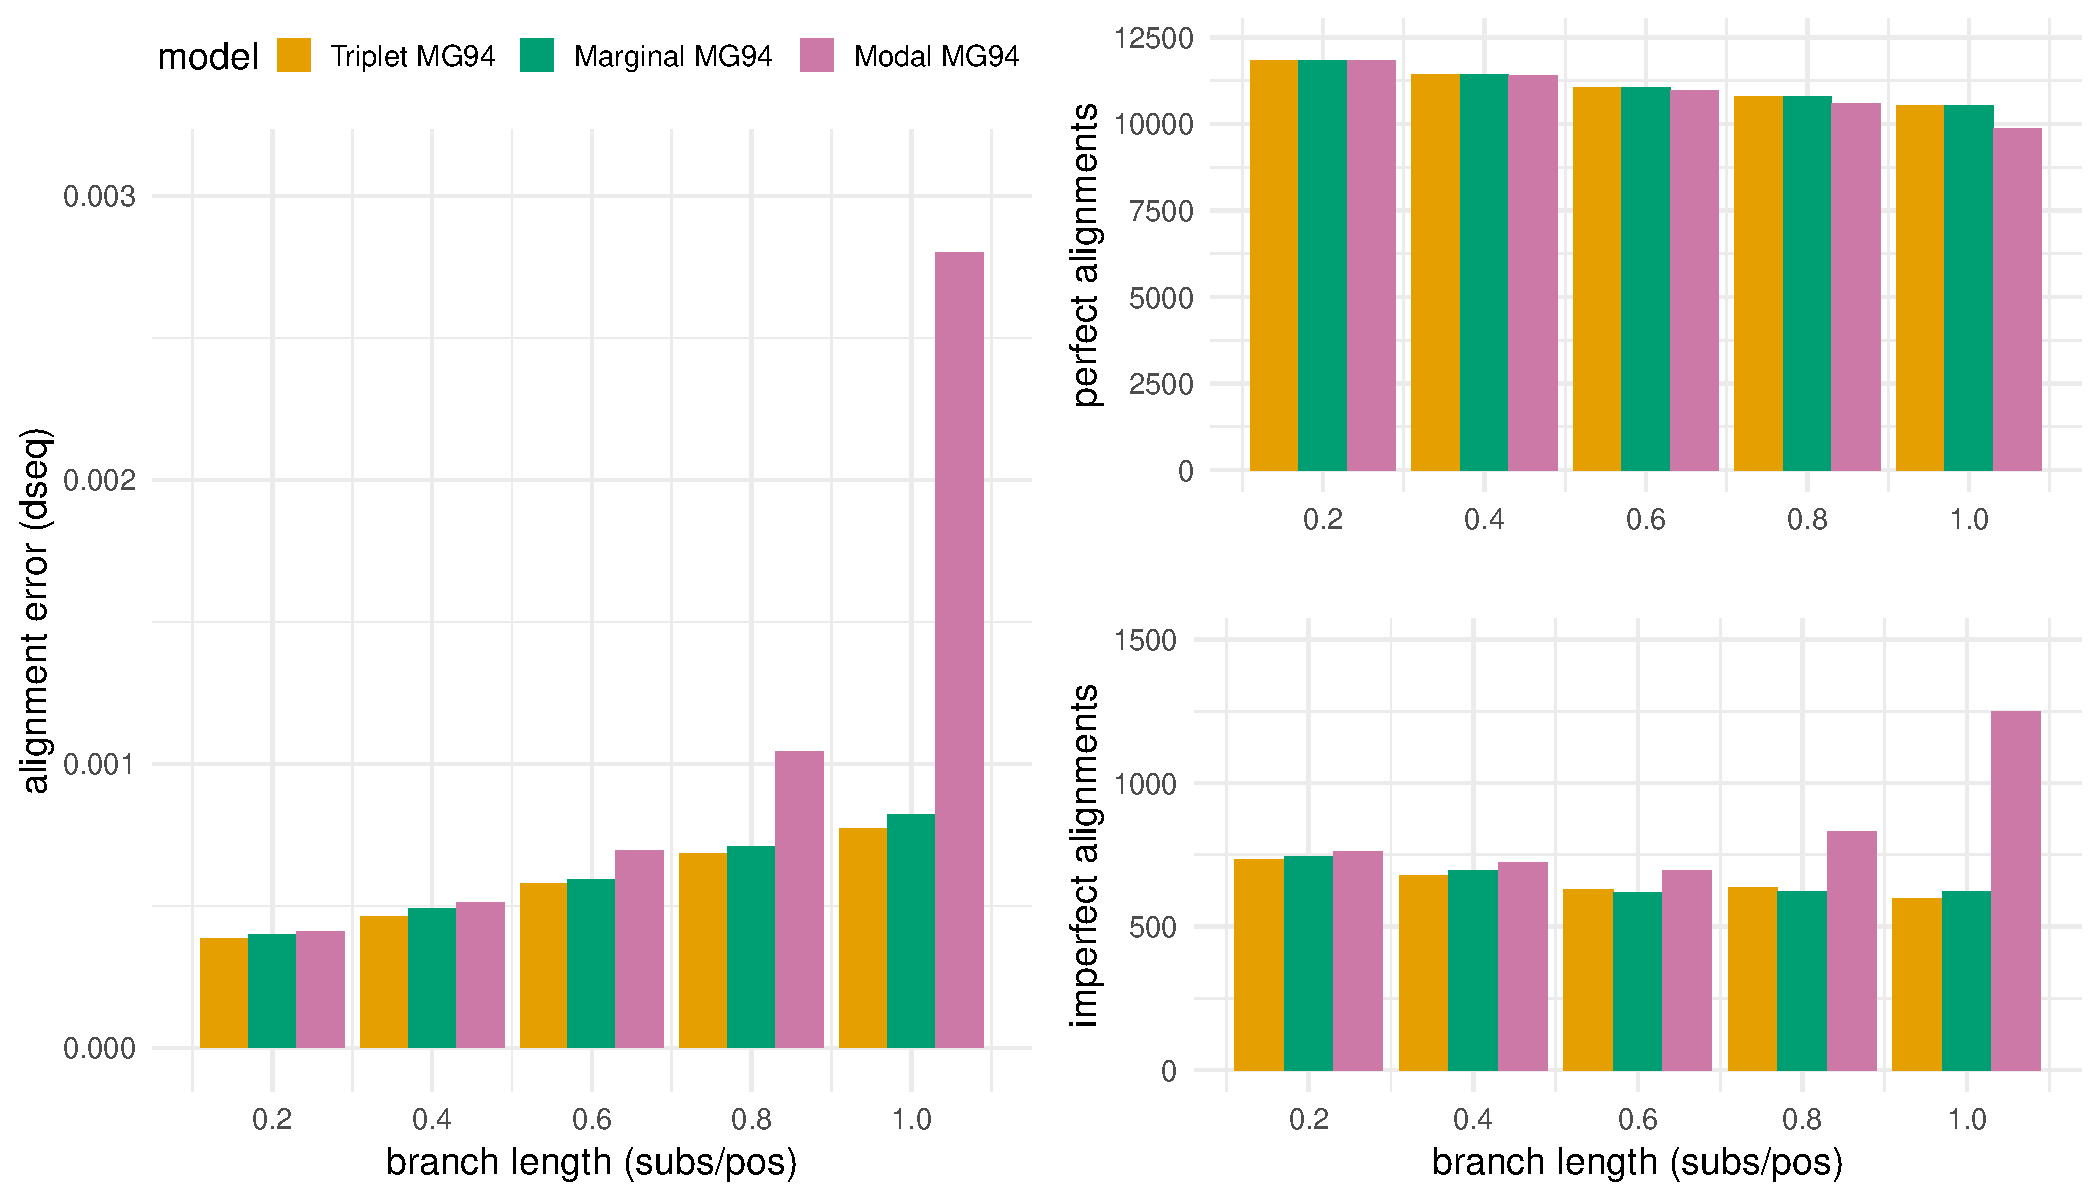
\includegraphics[width=\linewidth]{chapter3/figures/results/results_marginal_triplet_mg.pdf}
 \vspace{1mm}
 \caption[Alignment Accuracy of the Triplet and Approximate MG94 Models]{\DIFaddFL{The triplet-mg model generates better alignments across all branch lengths. Results of triplet-mg, marginal-mg, and modal-mg COATi models in aligning 13,758 simulated sequence pairs. Best alignments have the lowest $d_{seq}$, perfect alignments have the same score as the true alignment or a zero $d_{seq}$, and imperfect alignments have a different score than true alignments when at least one model found a perfect alignment.}}
 \label{fig:results_tri_mar_mg}
\end{figure}

\DIFadd{The number of perfect alignments between the marginal-mg and triplet-mg model remains consistent across all branch lengths. In contrast, the marginal-mg starts producing an equal number of perfect alignments for a branch length of $0.2$, but this number declines as branch lengths increase. A similar trend is observed in the count of imperfect alignments, with the modal-mg model producing more imperfect alignments, particularly spiking at branch lengths of $0.8$ and $1.0$. In this section, the remaining models performed similarly, with the marginal-mg model outperforming the triplet-mg model with branch lengths $0.6$ and $0.8$, with the reverse outcome for branch lengths $0.2$, $0.4$, and $1.0$. Note that the count of perfect and imperfect alignments decreases along the x-axis, as alignments not perfectly retrieved by either method are excluded from the results.
}

\subsubsection{\DIFadd{ECM}}

\DIFadd{As expected, the triplet-ecm model outperforms the marginal models across all branch lengths in all metrics (Fig.~\ref{fig:results_tri_mar_ecm}). The trend observed in the MG94 results is intensified in the ECM results. The $d_{seq}$ values for the triplet-ecm and marginal-ecm models are comparable to their MG94 counterparts, albeit with a slightly larger difference between them. This pattern is also evident in the number of perfect and imperfect alignments, where the triplet-ecm model significantly outperforms the approximate models. However, the marginal-ecm model provides a better approximation. In contrast, the modal-ecm model underperforms with a $d_{seq}$ two orders of magnitude larger than its MG94 counterpart for a branch length of 1. The model struggles with short branch lengths, and its performance declines as the number of expected substitutions per site increases. I have truncated the $d_{seq}$ values at $0.05$ to ensure a proper display of the results for the triplet-ecm and marginal-ecm. A comprehensive results table can be found in the appendix (Table \ref{table:results-ecm}).
}

\begin{figure}[!ht]
\centering
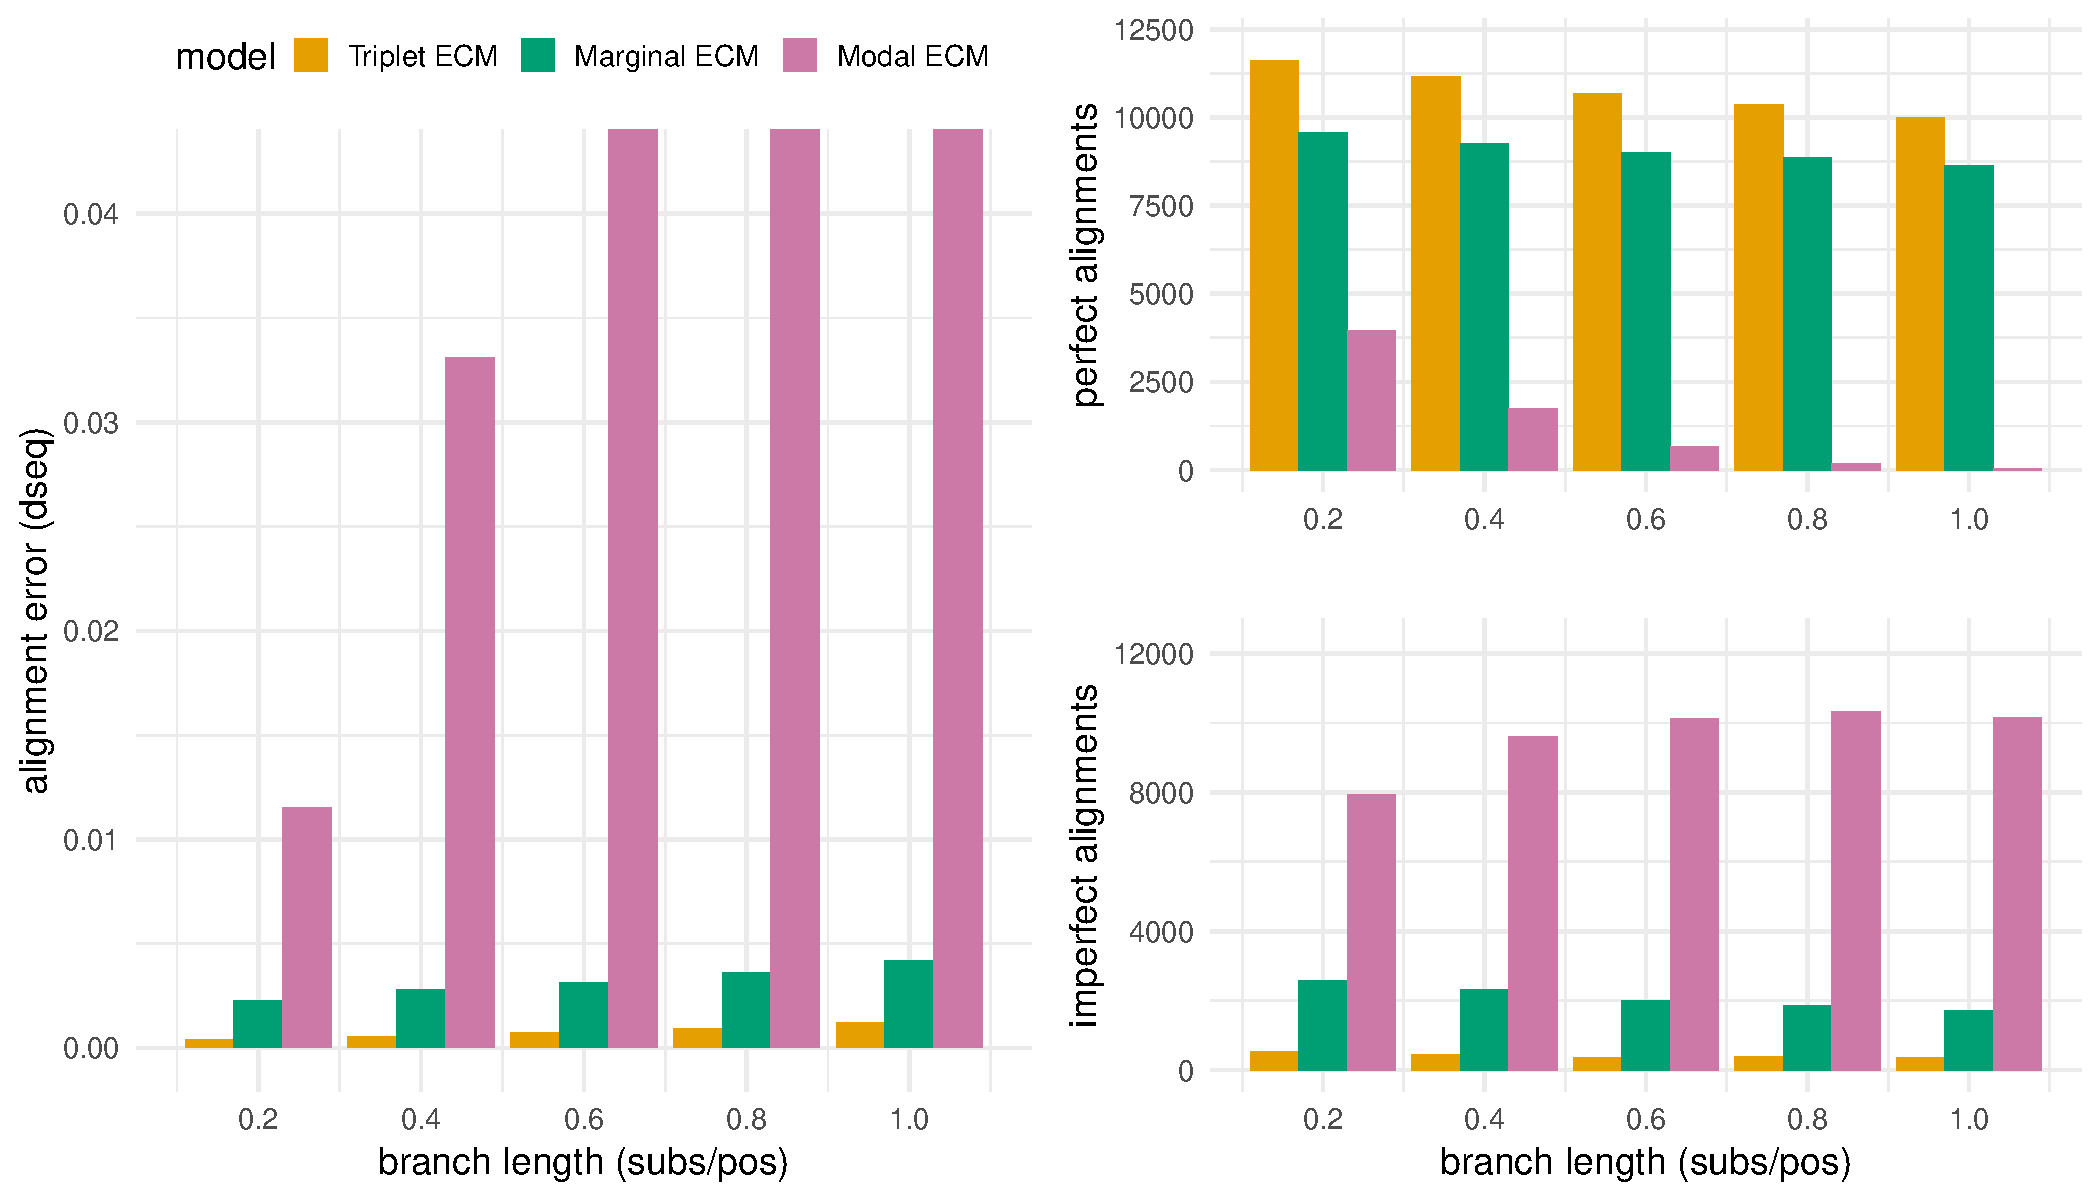
\includegraphics[width=\linewidth]{chapter3/figures/results/results_marginal_triplet_ecm.pdf}
 \vspace{1mm}
 \caption[Alignment Accuracy of the Triplet and Approximate ECM Models]{\DIFaddFL{The triplet-ecm model generates better alignments across all branch lengths. Results of triplet-ecm, modal-ecm, and marginal-ecm COATi models in aligning 13,758 simulated sequence pairs. Best alignments have the lowest $d_{seq}$, perfect alignments have the same score as the true alignment or a zero $d_{seq}$, and imperfect alignments have a different score than true alignments when at least one model found a perfect alignment.}}
 \label{fig:results_tri_mar_ecm}
\end{figure}

\subsection{\DIFadd{Gap Statistics}} %DIF > %%%%%%%%%%%%%%%%%%%%%%%%%%%%%%%%%%%%%%%%%%%%%%%%%%%%%%%%%%%%%

\DIFadd{Gap statistics can provide valuable insights when comparing alignment models across varying evolutionary distances, as they reveal how the likelihood of substitution relative to indel probabilities changes. Notably, for both the MG94 and ECM models, the total number of gaps and their cumulative length remains constant for both the triplet and marginal models as branch lengths increase (Fig.~\ref{fig:results_tri_mar_mg_gaps}). In concordance with the previous metrics, the behavior of the modal model takes a divergent path, especially for modal-ecm. While the modal-mg model shows similar values until branch length reaches $0.6$ and is slightly elevated thereafter, the total number and length of gaps for the modal-ecm model are larger for all branch lengths.
}

\begin{figure}[!ht]
\centering
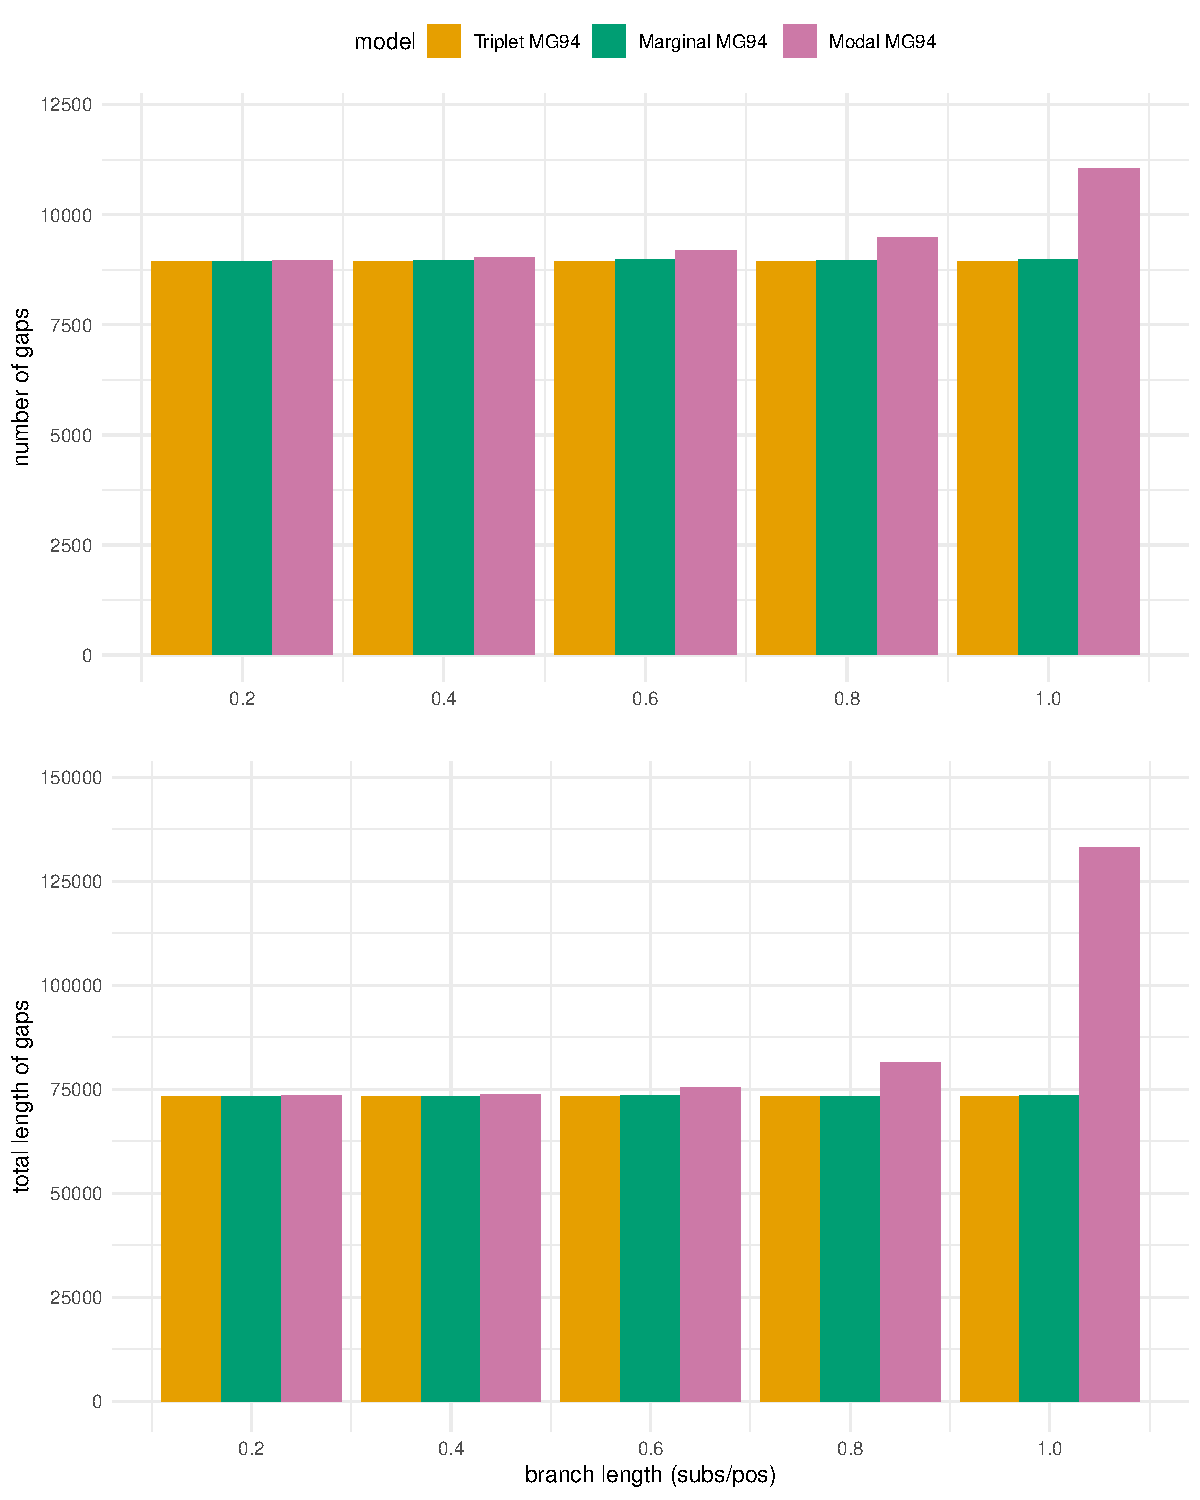
\includegraphics[width = 0.75\linewidth]{chapter3/figures/results/results_marginal_triplet_mg_gaps.pdf}
 \vspace{1mm}
 \caption[MG94 Dataset Indel Statistics]{\DIFaddFL{The number and total length of gaps for triplet-mg and marginal-mg models stay constant as branch lengths increase. On the contrary, the modal-mg model adds more and longer gaps as the evolutionary distance between sequences becomes larger.}}
 \label{fig:results_tri_mar_mg_gaps}
\end{figure}

\begin{figure}[!ht]
\centering
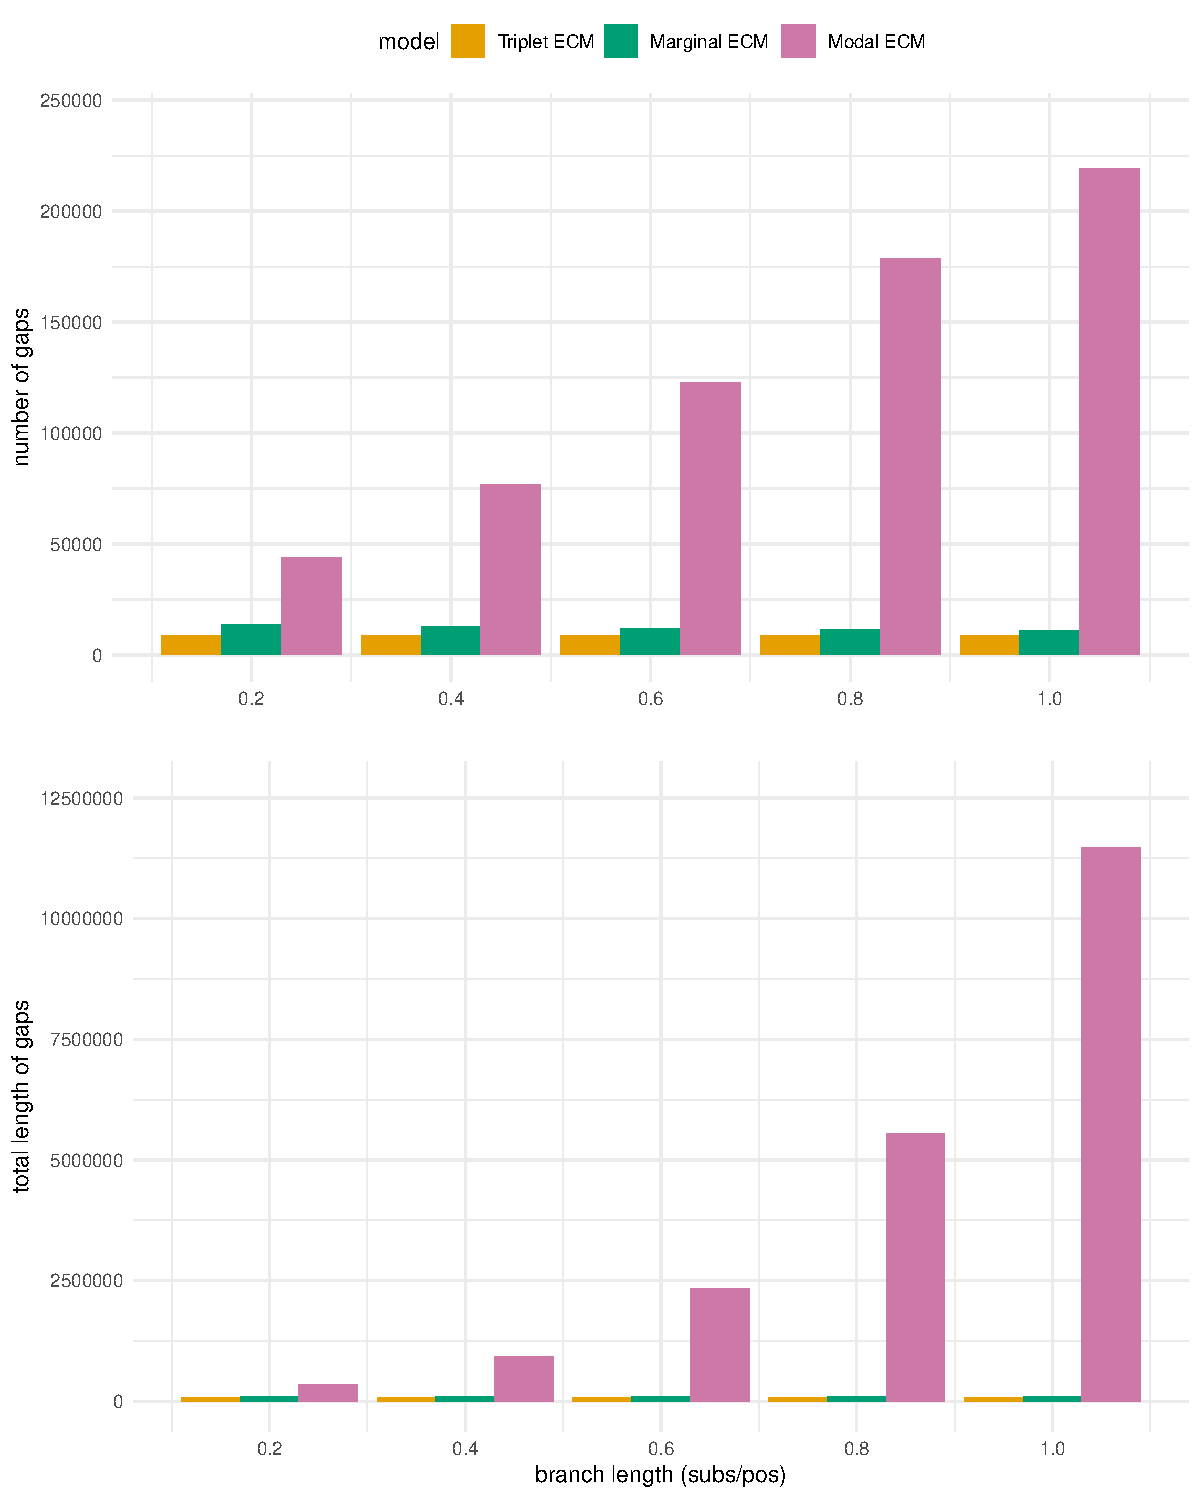
\includegraphics[width = 0.75\linewidth]{chapter3/figures/results/results_marginal_triplet_ecm_gaps.pdf}
 \vspace{1mm}
 \caption[ECM Dataset Indel Statistics]{\DIFaddFL{The number and total length of gaps for triplet-ecm and marginal-ecm models stay constant as branch lengths increase. On the contrary, the modal-ecm model significantly adds more and longer gaps as the evolutionary distance between sequences becomes larger.}}
 \label{fig:results_tri_mar_ecm_gaps}
\end{figure}

\clearpage

\subsection{\DIFadd{Marginal Model}}

\DIFadd{The results from the previous section establish the marginal model as a close approximation to the triplet model. To better understand how marginalization influences the substitution probabilities}\DIFaddend , I plotted the Kullback-Leibler \DIFaddbegin \DIFadd{divergence }\DIFaddend ($D_{KL}$) \DIFdelbegin \DIFdel{divergence between them }\DIFdelend \DIFaddbegin \DIFadd{between the marginal }\DIFaddend and the triplet model. This score can be seen as the measure of how one probability distribution, the marginal, differs from a reference probability distribution, the triplet. Figure \ref{fig:kld} \DIFdelbegin \DIFdel{-top }\DIFdelend is a plot of $D_{KL}$ for the MG94 marginal \DIFaddbegin \DIFadd{(top) and ECM marginal (bottom) }\DIFaddend models with branch \DIFdelbegin \DIFdel{lengths values from 0.2 }\DIFdelend \DIFaddbegin \DIFadd{length values from 0.1 }\DIFaddend to 10. \DIFdelbegin \DIFdel{Marginal-sum-mg is a better approximation, with smaller divergence values for all branch lengths. While at the starting branch length of $0.2$ both models have a similar divergence, the values }\DIFdelend \DIFaddbegin \DIFadd{The divergence }\DIFaddend for \DIFdelbegin \DIFdel{marginal-max-mg increase rapidly. Values for both models increase }\DIFdelend \DIFaddbegin \DIFadd{both marginal models follows a similar trend, with values rising }\DIFaddend until they reach saturation \DIFdelbegin \DIFdel{, where ultimately their divergence with MG94 decreases. Figure \ref{fig:kld}-bottom shows a similar pattern for the ECM case. Marginal-sum-ecm also performs best }\DIFdelend \DIFaddbegin \DIFadd{to then tend towards zero. Marginal-mg is a better approximation to its triplet counterpart than marginal-ecm with smaller values }\DIFaddend across all branch lengths\DIFdelbegin \DIFdel{, with similar values to marginal-max-ecm for a branch length of $0.2$. However, both ECM marginal models have a more pronounced curve than their MG94 counterparts, reaching higher divergence values. Additionally, marginal-sum-ecm and marginal-max-ecm reach saturation and their $D_{KL}$ tends towards zero.
}\DIFdelend \DIFaddbegin \DIFadd{.
%DIF >  Sum-mg is a better approximation, with smaller divergence values for all branch lengths. While at the starting branch length of $0.2$ both models have a similar divergence, the values for max-mg increase rapidly. Values for both models increase until they reach saturation, where ultimately their divergence with MG94 decreases.
%DIF >  Figure \ref{fig:kld}-bottom shows a similar pattern for the ECM case. Sum-ecm also performs best across all branch lengths, with similar values to max-ecm for a branch length of $0.2$. However, both ECM marginal models have a more pronounced curve than their MG94 counterparts, reaching higher divergence values. Additionally, sum-ecm and max-ecm reach saturation and their $D_{KL}$ tends towards zero.
}\DIFaddend 

% I analyzed the mutation rates of the triplet model at different branch lengths. The substitution probabilities are plotted in a 61 by 61 matrix, representing codon-to-codon rates, with values ranging from 0 to 1. In this matrix, each column corresponds to the probabilities of a specific codon being replaced by any of the other 61. By definition, shorter branch lengths equate to a small number of expected substitutions per position. Consequently, the majority of the probabilities in the matrix are concentrated along the main diagonal (Fig.~\ref{fig:ptri-02}), indicating substitutions are most likely to retain the same codon.

% Conversely, with longer branch lengths, the distribution of probabilities within each column is not concentrated in one cell and becomes more scattered. Notably, transitions and transversions in the third position of each codon become visible and distinguishable from each other as they begin accumulating probability mass, with transition harnessing a higher probability (Fig.~\ref{fig:ptri-08}). In addition, the increase of first and second-position transition probabilities becomes noticeable.

\begin{figure}[!ht]
    \centering
    \DIFdelbeginFL %DIFDELCMD < 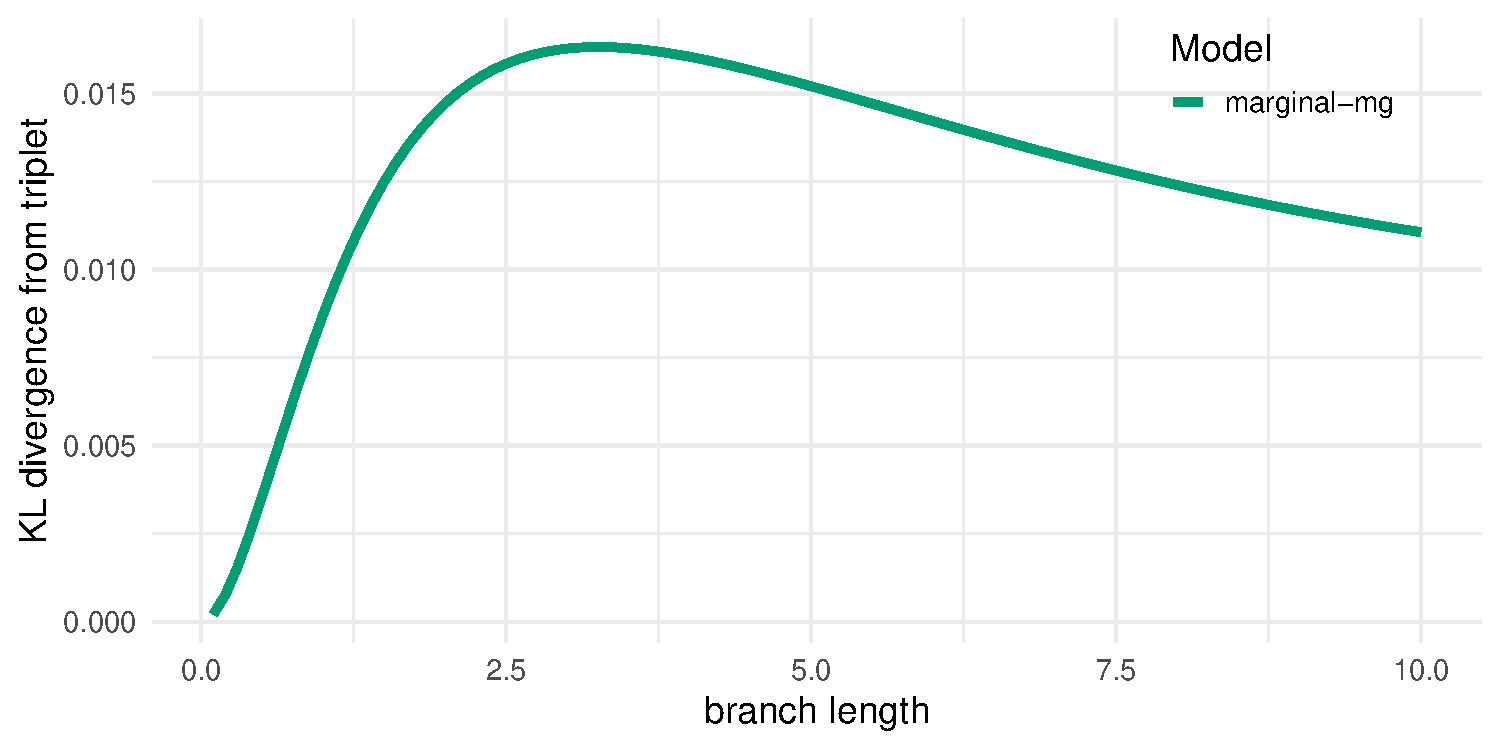
\includegraphics[width = 0.7\textwidth]{chapter3/figures/heatmaps/kld_mg.pdf}
%DIFDELCMD <     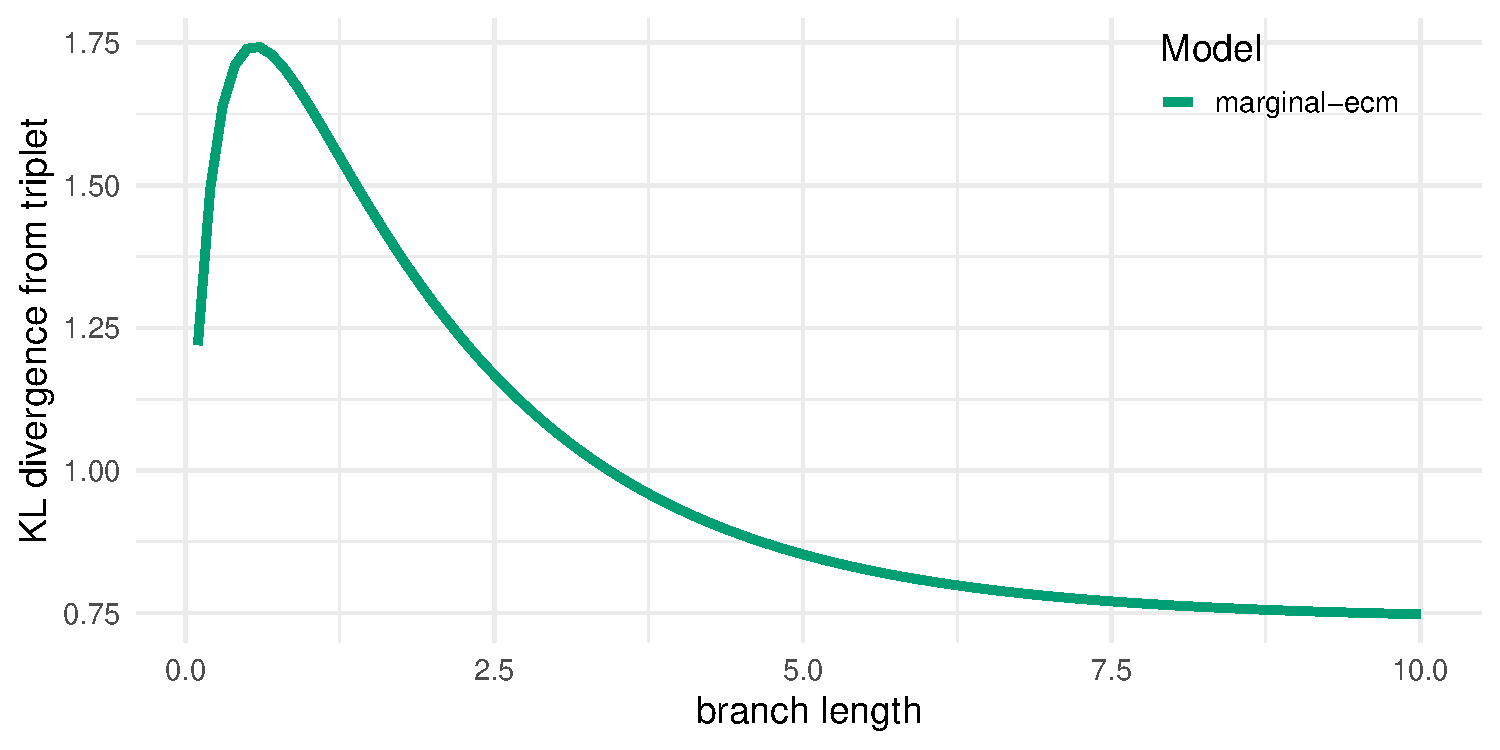
\includegraphics[width = 0.7\textwidth]{chapter3/figures/heatmaps/kld_ecm.pdf}
%DIFDELCMD <     %%%
\DIFdelendFL \DIFaddbeginFL 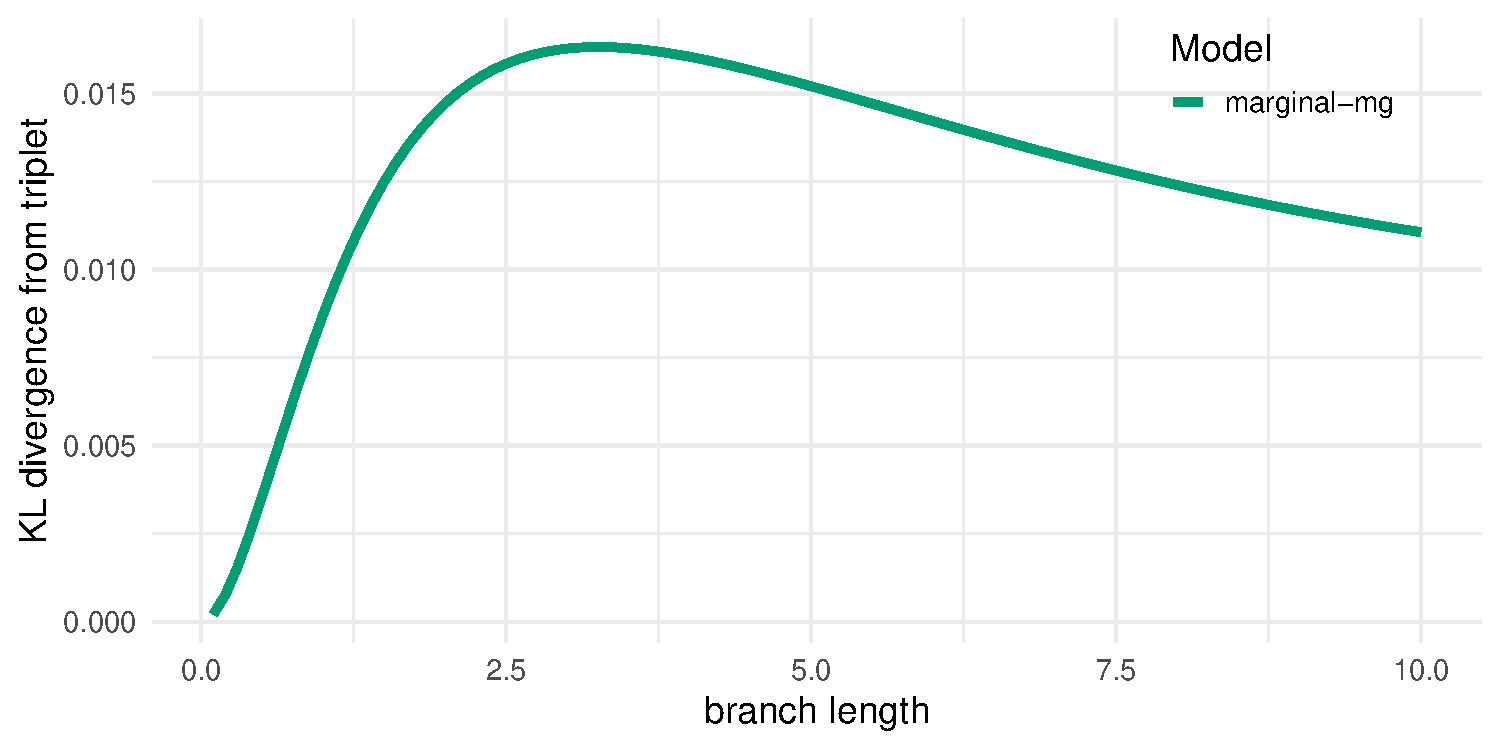
\includegraphics[width = 0.9\textwidth]{chapter3/figures/heatmaps/kld_mg.pdf}
    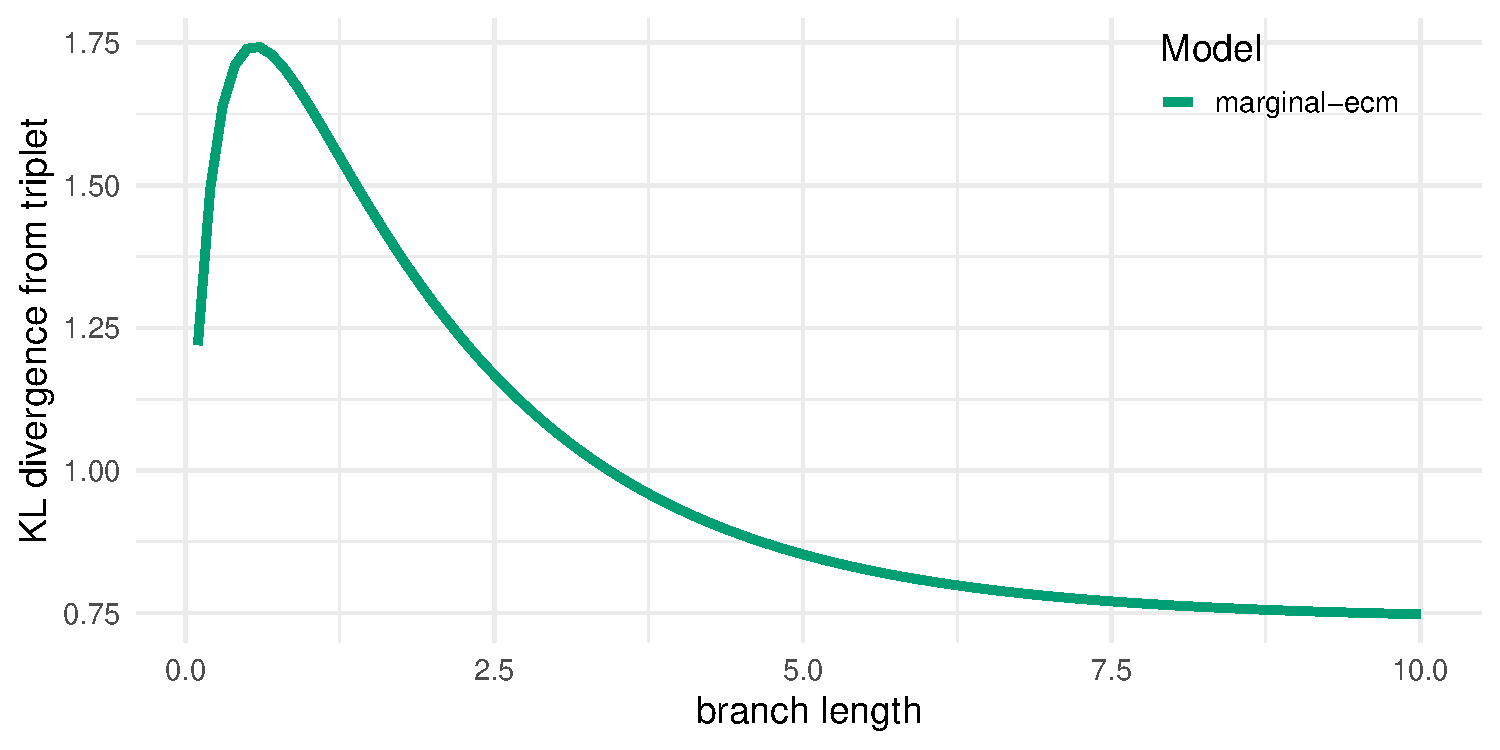
\includegraphics[width = 0.9\textwidth]{chapter3/figures/heatmaps/kld_ecm.pdf}
    \DIFaddendFL \caption[Marginal KL Divergence]{Kullback-Leibler divergence between MG94 (top) ECM (bottom) and their marginal models with branch lengths between 0.2 and 10. Low values represent a small divergence, indicating a better approximation to the triplet model. \DIFdelbeginFL \DIFdelFL{Marginal-sum }\DIFdelendFL \DIFaddbeginFL \DIFaddFL{Marginal MG94 }\DIFaddendFL performs best, while the divergence for both models decreases as they reach saturation.}
    \label{fig:kld}
\end{figure}

In addition to the overall measure of divergence, I plotted the $D_{KL}$ \DIFdelbegin \DIFdel{matrices }\DIFdelend \DIFaddbegin \DIFadd{matrix }\DIFaddend between the triplet and marginal \DIFdelbegin \DIFdel{models }\DIFdelend \DIFaddbegin \DIFadd{model }\DIFaddend at a branch length of 1 to understand what substitutions drive this score. \DIFdelbegin \DIFdel{These }\DIFdelend \DIFaddbegin \DIFadd{This }\DIFaddend 61 by 61 matrix \DIFdelbegin \DIFdel{plots represent }\DIFdelend \DIFaddbegin \DIFadd{plot represents }\DIFaddend individual divergence values calculated using $D_{KL}$ (Eq. \ref{eq:KLD}), where blue cells indicate substitution probabilities that are underestimated by the marginal model, while red cells indicate overestimation.
\DIFdelbegin \DIFdel{Figure \ref{fig:kld-max-mg} }\DIFdelend %DIF >  Figure \ref{fig:kld-max-mg} shows the divergence scores for the max MG94 model. The divergence in this model is driven by a general overestimation along the main diagonal and for first and third-position changes. The most underestimated amino acids are tyrosine and leucine, as shown by a blue predominant section in the top right of the figure, and the most overestimated amino acid is arginine, depicted by a red square along the main diagonal.
\DIFaddbegin \DIFadd{Figure \ref{fig:kld-sum-mg} }\DIFaddend shows the divergence scores for the \DIFdelbegin \DIFdel{marginal-max MG94 }\DIFdelend \DIFaddbegin \DIFadd{marginal }\DIFaddend model. The divergence \DIFdelbegin \DIFdel{in this model is driven by a general overestimation along the main diagonal and for first and third-position changes. The most underestimated amino acids are tyrosine and leucine, as shown by a blue predominant section in the top right of the figure, and the most overestimated amino acid is arginine, depicted by a red square along the main diagonal. The divergence for the other marginal MG94 model, marginal-sum, }\DIFdelend is driven by a combination of an underestimation of transversions and an overestimation of transitions on the first and third-position mutations\DIFdelbegin \DIFdel{(Fig. \ref{fig:kld-sum-mg}). Note that the divergence is two orders of magnitude smaller than for the marginal-max-mg.
}\DIFdelend \DIFaddbegin \DIFadd{.
%DIF >  Note that the divergence is two orders of magnitude smaller than for the max-mg.
}\DIFaddend In this case, the most underestimated amino acids are Leucine and Serine, while the most overestimated are tryptophan and tyrosine.

The divergence \DIFdelbegin \DIFdel{matrices }\DIFdelend \DIFaddbegin \DIFadd{matrix }\DIFaddend for the ECM \DIFdelbegin \DIFdel{models are }\DIFdelend \DIFaddbegin \DIFadd{model is }\DIFaddend plotted following the codon order used in the original ECM publication \citep{kosiol_ECM_2007}, where the order of nucleotides is \{T, C, A, G\}, and first position changes precede second position ones \DIFdelbegin \DIFdel{. The }\DIFdelend \DIFaddbegin \DIFadd{(Fig. \ref{fig:kld-sum-ecm}).
%DIF >  The divergence for the max-ecm model is driven by a general overestimation of substitution probabilities, especially along the main diagonal. A blue section on the top right corner portrays an underestimation zone, with amino acids arginine and serine being the most underestimated by this model.
The $D_{KL}$ }\DIFaddend divergence for the \DIFdelbegin \DIFdel{marginal-max-ecm }\DIFdelend \DIFaddbegin \DIFadd{marginal-ecm }\DIFaddend model is driven by a general overestimation of substitution probabilities, especially along the main diagonal \DIFdelbegin \DIFdel{. A blue section on the top right corner portrays an underestimation zone, with amino acids arginine and serine being the most underestimated by this model. Finally, the $D_{KL}$ divergence for the marginal-sum model follows the trend of the marginal-max-ecm, with a general overestimation of substitution probabilities and }\DIFdelend \DIFaddbegin \DIFadd{(indicating no change). In addition, we observe }\DIFaddend an underestimation of the arginine and serine amino acids (top left blue section). \DIFdelbegin \DIFdel{In both marginal models, the top }\DIFdelend \DIFaddbegin \DIFadd{The }\DIFaddend most overestimated amino acids include histidine, although the difference is small. \DIFdelbegin \DIFdel{In addition, note that while }\DIFdelend \DIFaddbegin \DIFadd{Notably, }\DIFaddend the divergence values \DIFdelbegin \DIFdel{between the max and sum marginal ECM models are on the same order of magnitude, these }\DIFdelend \DIFaddbegin \DIFadd{for the marginal ECM model }\DIFaddend are much higher than for the MG94 \DIFdelbegin \DIFdel{counterparts}\DIFdelend \DIFaddbegin \DIFadd{counterpart}\DIFaddend .

\DIFdelbegin %DIFDELCMD < \begin{figure}[!ht]
%DIFDELCMD <     \centering
%DIFDELCMD <     %%%
%DIF <  \includegraphics[width = 0.8\textwidth]{chapter3/figures/heatmaps/tri-max-mg-0.2.pdf}
    %DIFDELCMD < 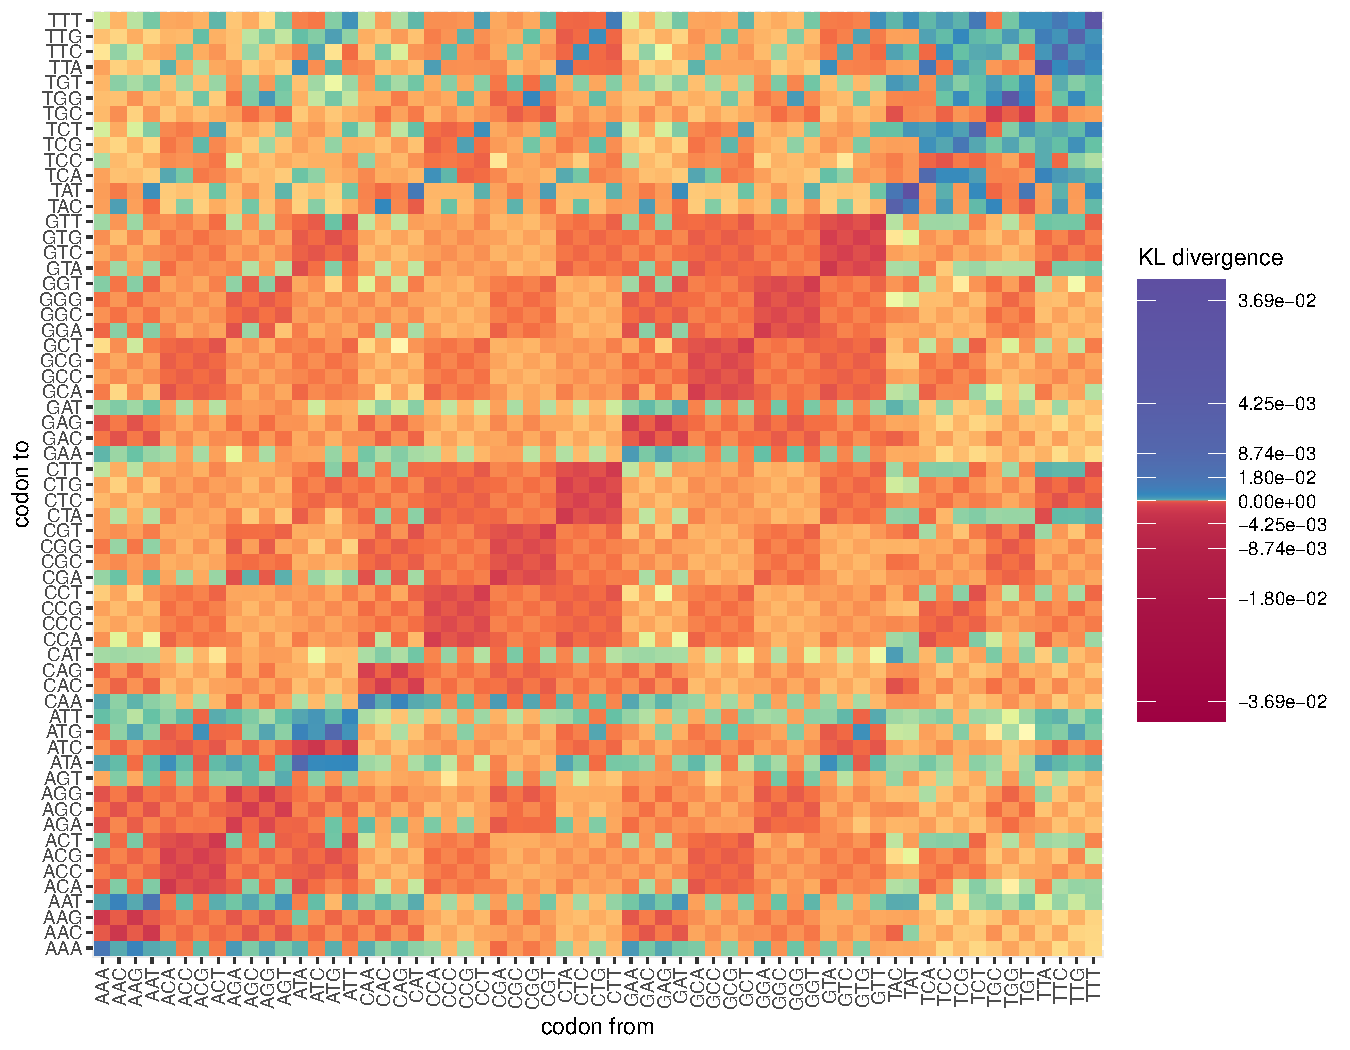
\includegraphics[width = \textwidth]{chapter3/figures/heatmaps/tri-max-mg-1.pdf}
%DIFDELCMD <     %%%
%DIFDELCMD < \caption[Marginal-max-mg Kullback-Leibler Divergence Matrix]{%
{%DIFAUXCMD
\DIFdelFL{Kullback-Leibler divergence matrix for the marginal-max MG94 model with a branch length of $1.0$. Values closer to zero indicate a smaller divergence, representing a better approximation to the triplet model. Positive values, indicated by a blue gradient, mark substitution probabilities where marginal-max underestimates the triplet model. In turn, negative values, indicated by a red gradient, represent substitution probabilities where marginal-max overestimates the triplet model.}}
    %DIFAUXCMD
%DIFDELCMD < \label{fig:kld-max-mg}
%DIFDELCMD < \end{figure}
%DIFDELCMD < %%%
\DIFdelend %DIF >  \begin{figure}[!ht]
%DIF >      \centering
%DIF >      % \includegraphics[width = 0.8\textwidth]{chapter3/figures/heatmaps/tri-max-mg-0.2.pdf}
%DIF >      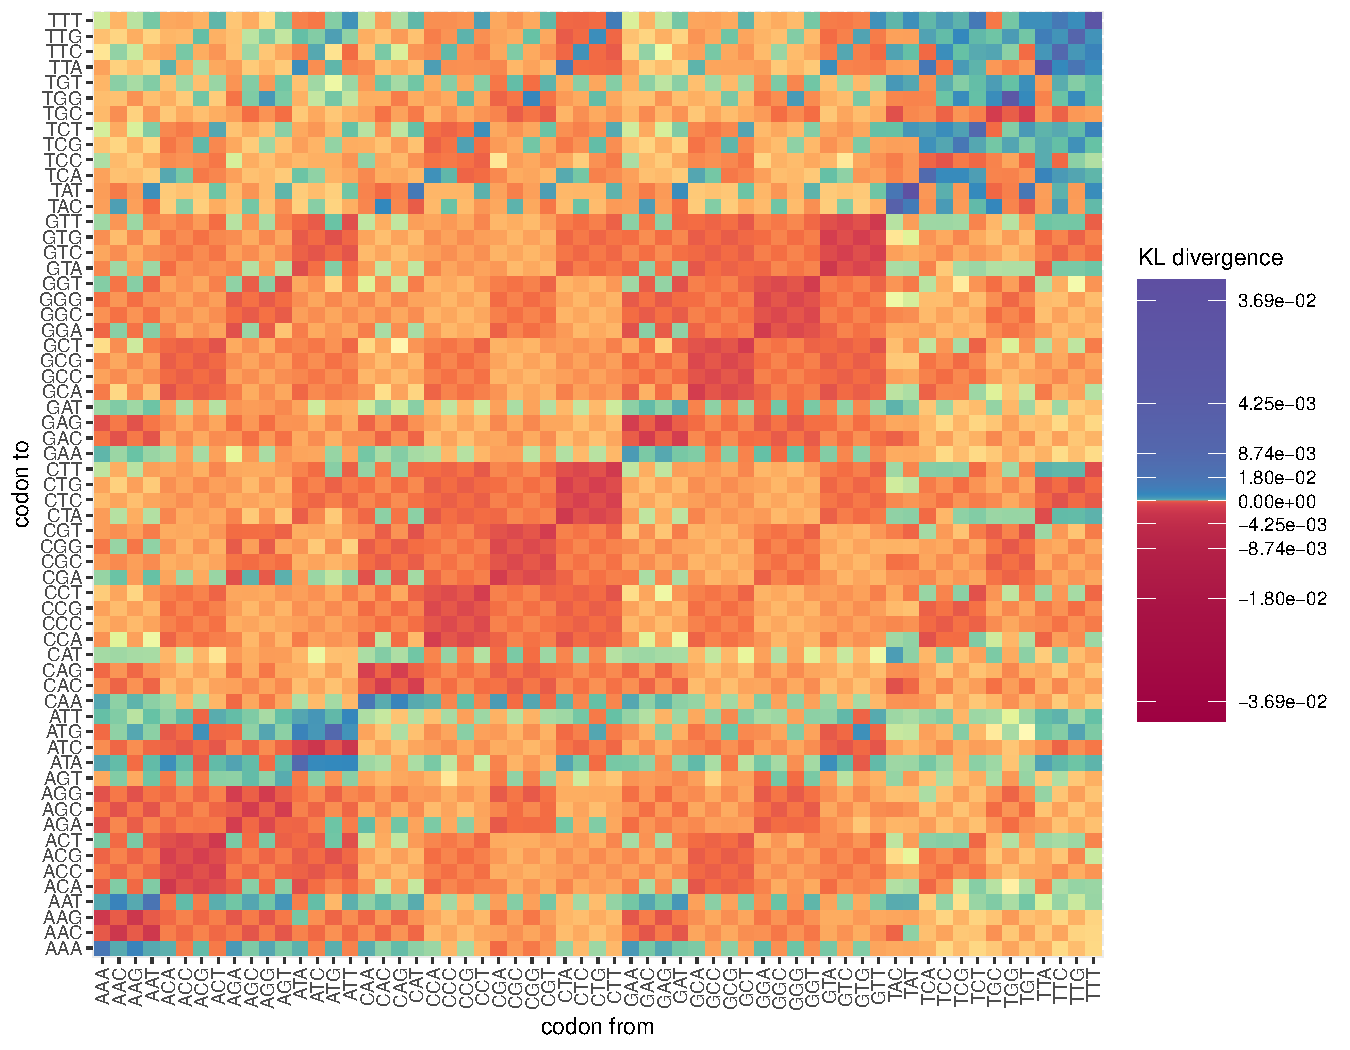
\includegraphics[width = \textwidth]{chapter3/figures/heatmaps/tri-max-mg-1.pdf}
%DIF >      \caption[Max-mg Kullback-Leibler Divergence Matrix]{Kullback-Leibler divergence matrix for the max MG94 model with a branch length of $1.0$. Values closer to zero indicate a smaller divergence, representing a better approximation to the triplet model. Positive values, indicated by a blue gradient, mark substitution probabilities where max underestimates the triplet model. In turn, negative values, indicated by a red gradient, represent substitution probabilities where max overestimates the triplet model.}
%DIF >      \label{fig:kld-max-mg}
%DIF >  \end{figure}

\begin{figure}[!ht]
    \centering
    % \includegraphics[width = 0.8\textwidth]{chapter3/figures/heatmaps/tri-sum-mg-0.2.pdf}
    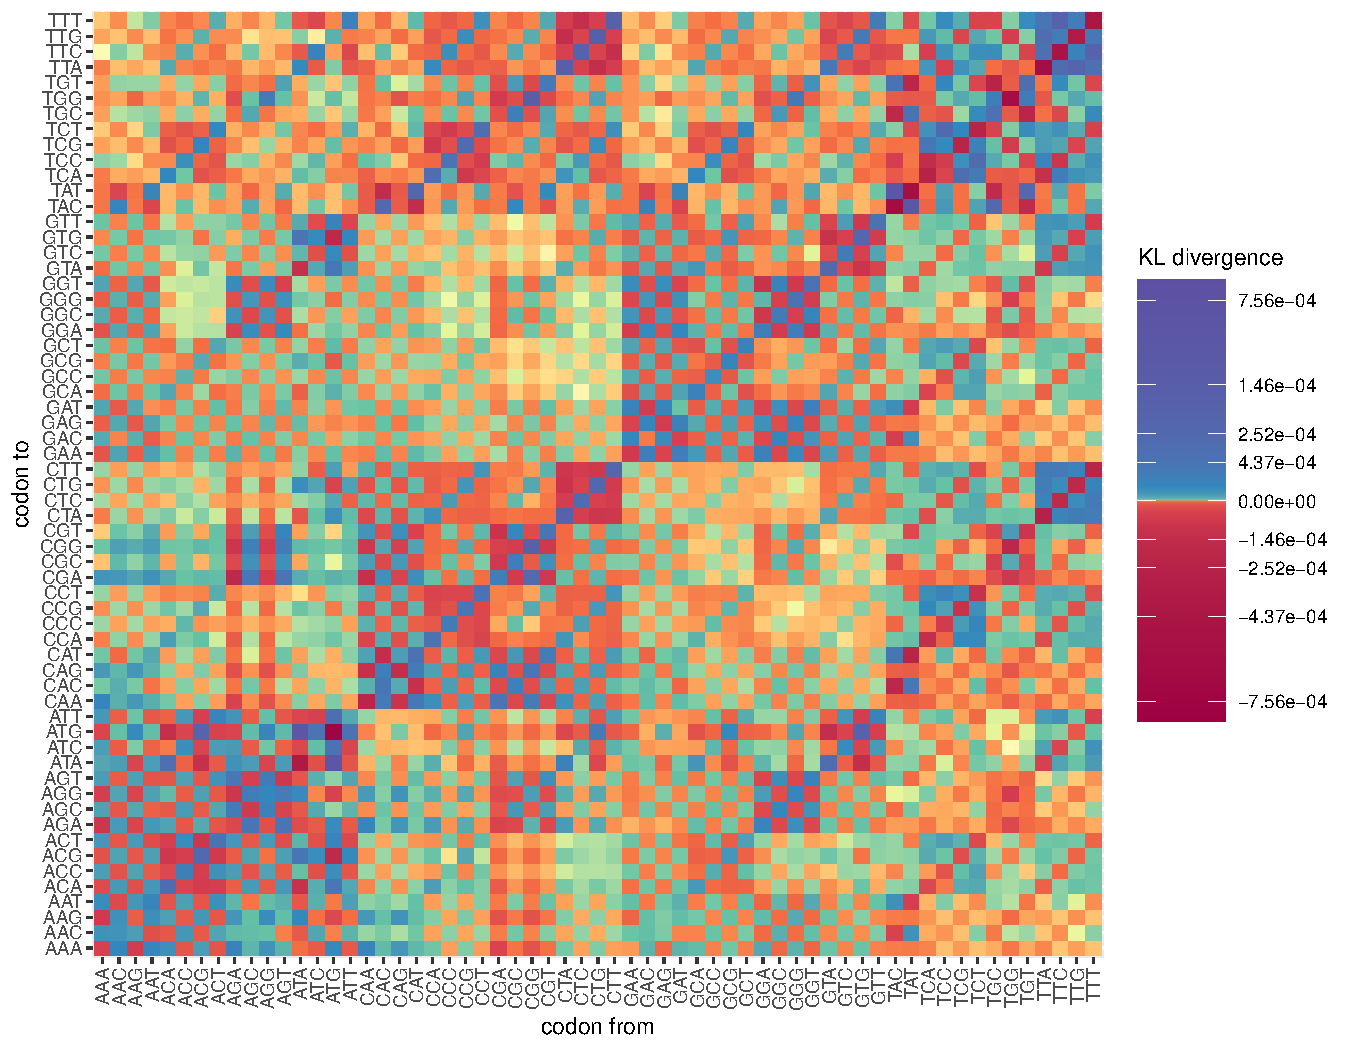
\includegraphics[width = \textwidth]{chapter3/figures/heatmaps/tri-sum-mg-1.pdf}
    \DIFdelbeginFL %DIFDELCMD < \caption[Marginal-sum-mg Kullback-Leibler Divergence Matrix]{%%%
\DIFdelendFL \DIFaddbeginFL \caption[Marginal-mg Kullback-Leibler Divergence Matrix]{\DIFaddendFL Kullback-Leibler divergence matrix for the \DIFdelbeginFL \DIFdelFL{marginal-sum }\DIFdelendFL \DIFaddbeginFL \DIFaddFL{marginal }\DIFaddendFL MG94 model with a branch length of $1.0$. Values closer to zero indicate a smaller divergence, representing a better approximation to the triplet model. Positive values, indicated by a blue gradient, mark substitution probabilities where \DIFdelbeginFL \DIFdelFL{marginal-sum }\DIFdelendFL \DIFaddbeginFL \DIFaddFL{the marginal model }\DIFaddendFL underestimates the triplet model. In turn, negative values, indicated by a red gradient, represent substitution probabilities where \DIFdelbeginFL \DIFdelFL{marginal-max }\DIFdelendFL \DIFaddbeginFL \DIFaddFL{marginal }\DIFaddendFL overestimates the triplet model.}
    \label{fig:kld-sum-mg}
\end{figure}

%DIF <  In addition to the overall measure of divergence, I analyzed the $D_{KL}$ matrix to understand what substitutions drive this score. Figure \ref{fig:kld-max-mg} shows the divergence scores for the marginal-max MG94 model at branch length $1.0$. The divergence in this model is driven by a combination of underestimating and overestimating the triplet along the main diagonal. Tyr is the most overestimated amino acid, while Arg is the most underestimated. For the marginal-sum MG94 model, figure \ref{fig:kld-sum-mg} shows the divergence with MG94 at a branch length of $1.0$. In this case, third and second-position transitions drive the divergence with the triplet model. Asn is the most overestimated amino acid, while Trp is the most underestimated.
%DIF >  In addition to the overall measure of divergence, I analyzed the $D_{KL}$ matrix to understand what substitutions drive this score. Figure \ref{fig:kld-max-mg} shows the divergence scores for the max MG94 model at branch length $1.0$. The divergence in this model is driven by a combination of underestimating and overestimating the triplet along the main diagonal. Tyr is the most overestimated amino acid, while Arg is the most underestimated. For the sum MG94 model, figure \ref{fig:kld-sum-mg} shows the divergence with MG94 at a branch length of $1.0$. In this case, third and second-position transitions drive the divergence with the triplet model. Asn is the most overestimated amino acid, while Trp is the most underestimated.

\DIFdelbegin %DIFDELCMD < \begin{figure}[!ht]
%DIFDELCMD <     \centering
%DIFDELCMD <     %%%
%DIF <  \includegraphics[width = 0.8\textwidth]{chapter3/figures/heatmaps/tri-max-mg-0.2.pdf}
    %DIFDELCMD < 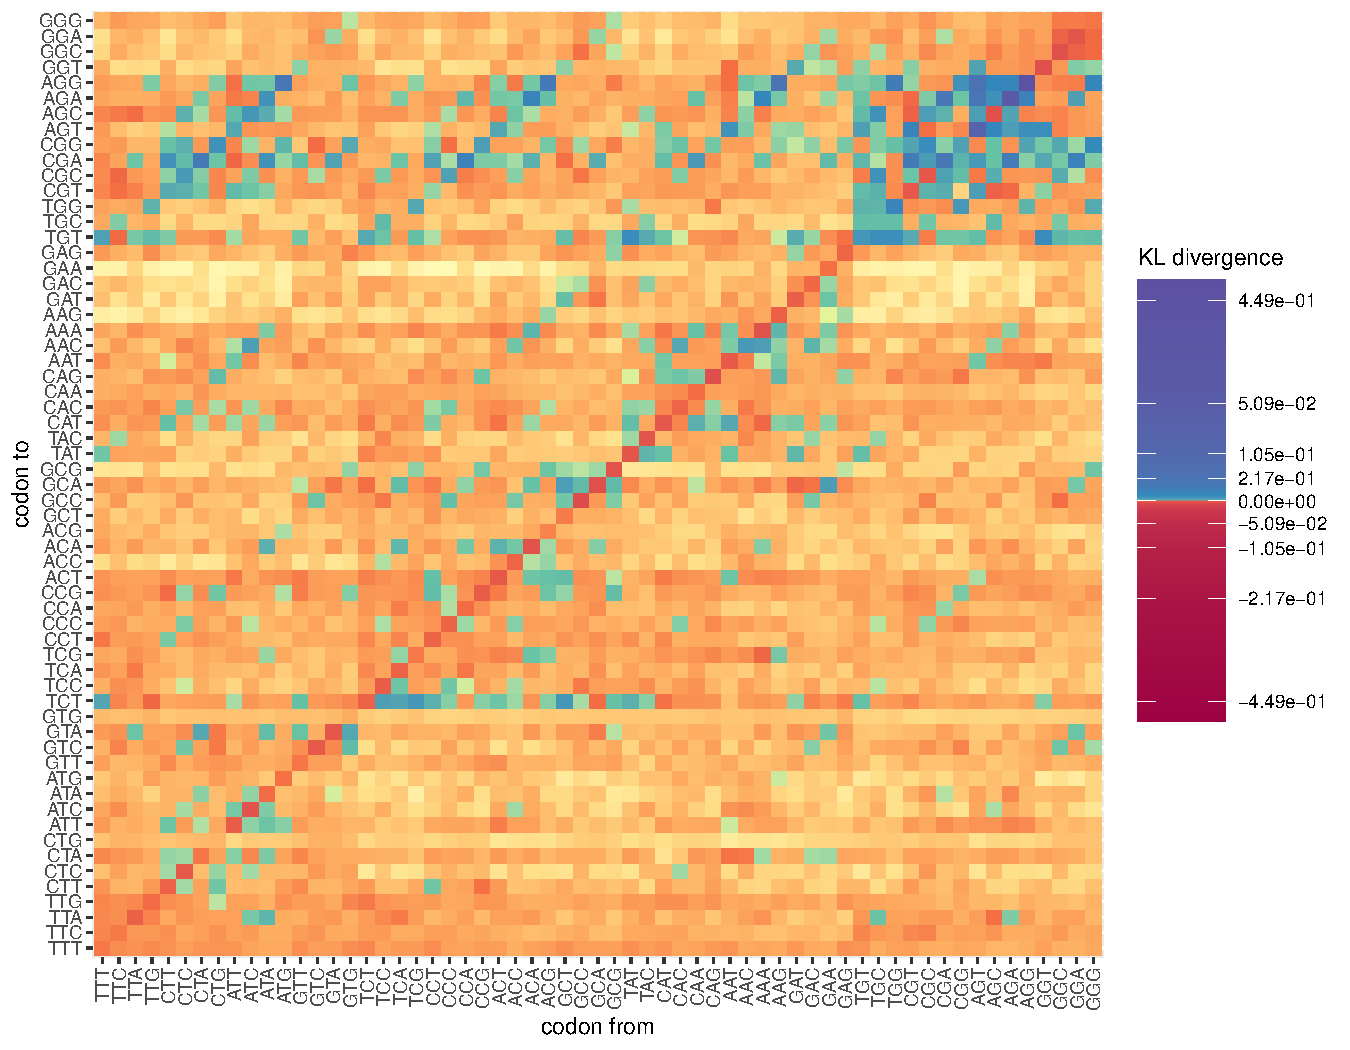
\includegraphics[width = \textwidth]{chapter3/figures/heatmaps/tri-max-ecm-1.pdf}
%DIFDELCMD <     %%%
%DIFDELCMD < \caption[Marginal-max-ecm Kullback-Leibler Divergence Matrix]{%
{%DIFAUXCMD
\DIFdelFL{Kullback-Leibler divergence matrix for the marginal-max ECM model with a branch length of $1.0$. Values closer to zero indicate a smaller divergence, representing a better approximation to the triplet model. Positive values, indicated by a blue gradient, mark substitution probabilities where marginal-max underestimates the triplet model. In turn, negative values, indicated by a red gradient, represent substitution probabilities where marginal-max overestimates the triplet model.}}
    %DIFAUXCMD
%DIFDELCMD < \label{fig:kld-max-ecm}
%DIFDELCMD < \end{figure}
%DIFDELCMD < %%%
\DIFdelend %DIF >  \begin{figure}[!ht]
%DIF >      \centering
%DIF >      % \includegraphics[width = 0.8\textwidth]{chapter3/figures/heatmaps/tri-max-mg-0.2.pdf}
%DIF >      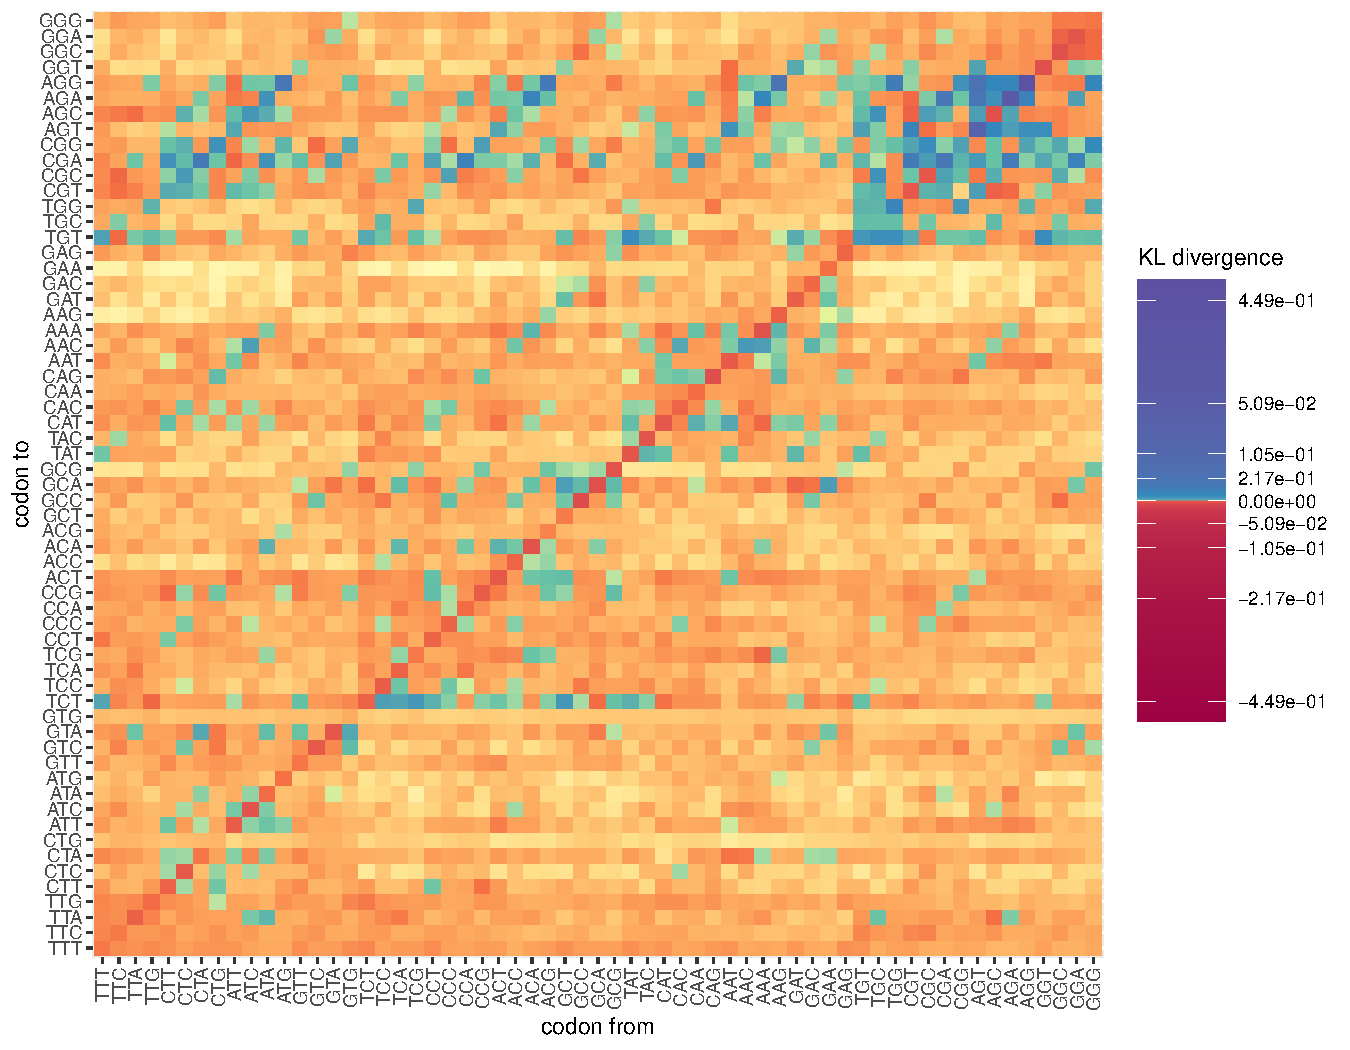
\includegraphics[width = \textwidth]{chapter3/figures/heatmaps/tri-max-ecm-1.pdf}
%DIF >      \caption[Max-ecm Kullback-Leibler Divergence Matrix]{Kullback-Leibler divergence matrix for the max ECM model with a branch length of $1.0$. Values closer to zero indicate a smaller divergence, representing a better approximation to the triplet model. Positive values, indicated by a blue gradient, mark substitution probabilities where max underestimates the triplet model. In turn, negative values, indicated by a red gradient, represent substitution probabilities where max overestimates the triplet model.}
%DIF >      \label{fig:kld-max-ecm}
%DIF >  \end{figure}

\begin{figure}[!ht]
    \centering
    % \includegraphics[width = 0.8\textwidth]{chapter3/figures/heatmaps/tri-sum-mg-0.2.pdf}
    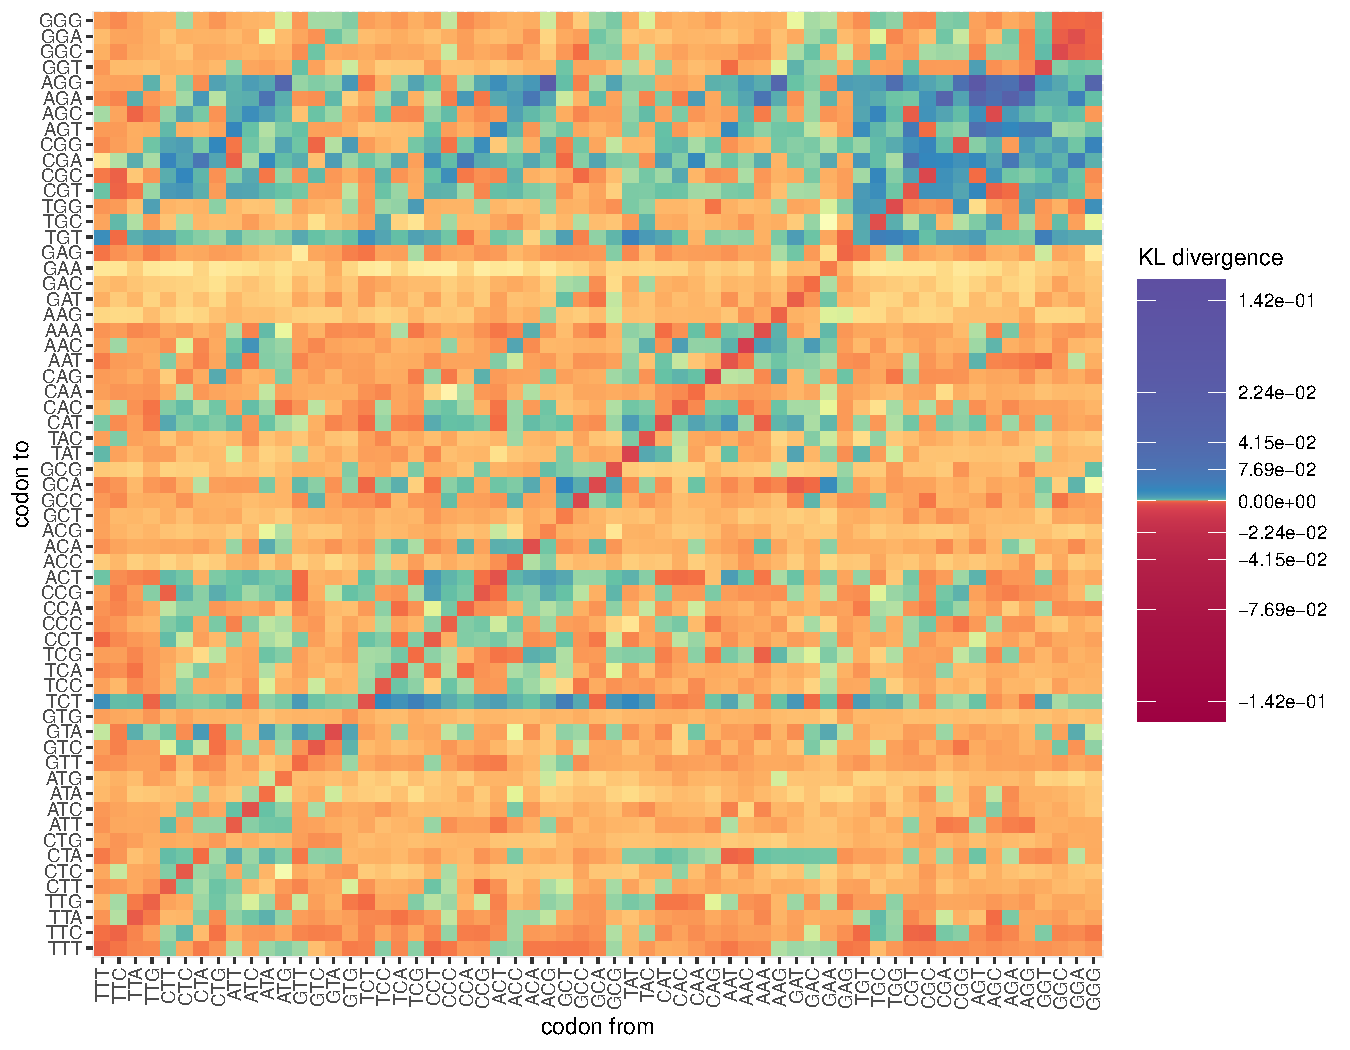
\includegraphics[width = \textwidth]{chapter3/figures/heatmaps/tri-sum-ecm-1.pdf}
    \DIFdelbeginFL %DIFDELCMD < \caption[Marginal-sum-ecm Kullback-Leibler Divergence Matrix]{%%%
\DIFdelendFL \DIFaddbeginFL \caption[Marginal-ecm Kullback-Leibler Divergence Matrix]{\DIFaddendFL Kullback-Leibler divergence matrix for the \DIFdelbeginFL \DIFdelFL{marginal-sum }\DIFdelendFL \DIFaddbeginFL \DIFaddFL{marginal }\DIFaddendFL ECM model with a branch length of $1.0$. Values closer to zero indicate a smaller divergence, representing a better approximation to the triplet model. Positive values, indicated by a blue gradient, mark substitution probabilities where \DIFdelbeginFL \DIFdelFL{marginal-sum }\DIFdelendFL \DIFaddbeginFL \DIFaddFL{the marginal model }\DIFaddendFL underestimates the triplet model. In turn, negative values, indicated by a red gradient, represent substitution probabilities where \DIFdelbeginFL \DIFdelFL{marginal-max }\DIFdelendFL \DIFaddbeginFL \DIFaddFL{marginal }\DIFaddendFL overestimates the triplet model.}
    \label{fig:kld-sum-ecm}
\end{figure}

\clearpage

\subsection{Visual \DIFdelbegin \DIFdel{comparison }\DIFdelend \DIFaddbegin \DIFadd{Comparison }\DIFaddend of \DIFdelbegin \DIFdel{triplet }\DIFdelend \DIFaddbegin \DIFadd{Triplet }\DIFaddend and \DIFdelbegin \DIFdel{marginal-sum}\DIFdelend \DIFaddbegin \DIFadd{Marginal Model}\DIFaddend } %%%%%%%%%%%%%%%%%%%%%

The previous metrics have demonstrated that the triplet and \DIFdelbegin \DIFdel{marginal-sum }\DIFdelend \DIFaddbegin \DIFadd{marginal }\DIFaddend models exhibit a strong agreement in their results, thereby validating the latter as a suitable approximation of the former. However, these metrics have fallen short in identifying any subtle distinctions between the models, if they exist. Pursuing these differences, I inspected the alignment sections where the two models diverge using dot plots. Upon visual comparison of the most distinct triplet and \DIFdelbegin \DIFdel{marginal-sum }\DIFdelend \DIFaddbegin \DIFadd{marginal }\DIFaddend alignments across sequence lengths spanning from a few hundred to a maximum of three thousand nucleotides and encompassing all branch lengths (0.2, 0.4, 0.6, 0.8, and 1.0), one predominant pattern emerges (examples in Fig.~\ref{fig:dotplots}). The most notable distinction between the triplet and \DIFdelbegin \DIFdel{marginal-sum }\DIFdelend \DIFaddbegin \DIFadd{marginal }\DIFaddend models lies in the former model displaying a preference for substitutions, irrespective of the number of matches, whereas the latter model favors indels, often with a higher number of matches (left column in Figure \ref{fig:dotplots}).

\begin{figure}[!ht]
 \centering
 % \setlength{\columnsep}{-4cm}
 \begin{multicols}{2}
% \vspace*{2.5em}
% \hspace{-5cm}
\DIFdelbeginFL %DIFDELCMD < \scalebox{0.52}{% Created by tikzDevice version 0.12.5 on 2023-10-05 23:41:42
%DIFDELCMD < % !TEX encoding = UTF-8 Unicode
%DIFDELCMD < \definecolor{triplet}{HTML}{E69F00}
%DIFDELCMD < \definecolor{mar-sum}{HTML}{009E73}
%DIFDELCMD < \definecolor{mar-max}{HTML}{CC79A7}
%DIFDELCMD < \definecolor{color1}{HTML}{CC9966}
%DIFDELCMD < \definecolor{color2}{HTML}{99CCFF}
%DIFDELCMD < \begin{tikzpicture}[dot/.style={circle, minimum size=2.5mm}, box/.style={rectangle, minimum size = 3.5cm, anchor = north west}]
%DIFDELCMD < \draw[very thin, color = gray!50, step = 0.5] (0,0) grid (10, 10);
%DIFDELCMD < \node at (0.25,9.25) {-};
%DIFDELCMD < \node at (0.25,8.75) {A};
%DIFDELCMD < \node at (0.25,8.25) {-};
%DIFDELCMD < \node at (0.25,7.75) {A};
%DIFDELCMD < \node at (0.25,7.25) {-};
%DIFDELCMD < \node at (0.25,6.75) {C};
%DIFDELCMD < \node at (0.25,6.25) {-};
%DIFDELCMD < \node at (0.25,5.75) {A};
%DIFDELCMD < \node at (0.25,5.25) {-};
%DIFDELCMD < \node at (0.25,4.75) {G};
%DIFDELCMD < \node at (0.25,4.25) {-};
%DIFDELCMD < \node at (0.25,3.75) {A};
%DIFDELCMD < \node at (0.25,3.25) {-};
%DIFDELCMD < \node at (0.25,2.75) {T};
%DIFDELCMD < \node at (0.25,2.25) {-};
%DIFDELCMD < \node at (0.25,1.75) {C};
%DIFDELCMD < \node at (0.25,1.25) {-};
%DIFDELCMD < \node at (0.25,0.75) {A};
%DIFDELCMD < \node at (0.25,0.25) {-};
%DIFDELCMD < \node at (0.75,9.75) {-};
%DIFDELCMD < \node at (1.25,9.75) {A};
%DIFDELCMD < \node at (1.75,9.75) {-};
%DIFDELCMD < \node at (2.25,9.75) {A};
%DIFDELCMD < \node at (2.75,9.75) {-};
%DIFDELCMD < \node at (3.25,9.75) {A};
%DIFDELCMD < \node at (3.75,9.75) {-};
%DIFDELCMD < \node at (4.25,9.75) {T};
%DIFDELCMD < \node at (4.75,9.75) {-};
%DIFDELCMD < \node at (5.25,9.75) {C};
%DIFDELCMD < \node at (5.75,9.75) {-};
%DIFDELCMD < \node at (6.25,9.75) {T};
%DIFDELCMD < \node at (6.75,9.75) {-};
%DIFDELCMD < \node at (7.25,9.75) {G};
%DIFDELCMD < \node at (7.75,9.75) {-};
%DIFDELCMD < \node at (8.25,9.75) {T};
%DIFDELCMD < \node at (8.75,9.75) {-};
%DIFDELCMD < \node at (9.25,9.75) {A};
%DIFDELCMD < \node at (9.75,9.75) {-};
%DIFDELCMD < \draw[line width=1.25mm,mar-sum](0.75,9.25)--(1.25,8.75);
%DIFDELCMD < \node[circle, fill=mar-sum] at (0.75, 9.25){};
%DIFDELCMD < \draw[line width=1.25mm,mar-sum](1.25,8.75)--(1.75,8.25);
%DIFDELCMD < \node[circle, fill=mar-sum] at (1.25, 8.75){};
%DIFDELCMD < \node[white] at (1.25, 8.75){$\mathlarger{\mathlarger{\bm{\times}}}$};
%DIFDELCMD < \draw[line width=1.25mm,mar-sum](1.75,8.25)--(2.25,7.75);
%DIFDELCMD < \node[circle, fill=mar-sum] at (1.75, 8.25){};
%DIFDELCMD < \draw[line width=1.25mm,mar-sum](2.25,7.75)--(2.75,7.25);
%DIFDELCMD < \node[circle, fill=mar-sum] at (2.25, 7.75){};
%DIFDELCMD < \node[white] at (2.25, 7.75){$\mathlarger{\mathlarger{\bm{\times}}}$};
%DIFDELCMD < \draw[line width=1.25mm,mar-sum](2.75,7.25)--(2.75,6.75);
%DIFDELCMD < \node[circle, fill=mar-sum] at (2.75, 7.25){};
%DIFDELCMD < \draw[line width=1.25mm,mar-sum](2.75,6.75)--(2.75,6.25);
%DIFDELCMD < \node[circle, fill=mar-sum] at (2.75, 6.75){};
%DIFDELCMD < \draw[line width=1.25mm,mar-sum](2.75,6.25)--(2.75,5.75);
%DIFDELCMD < \node[circle, fill=mar-sum] at (2.75, 6.25){};
%DIFDELCMD < \draw[line width=1.25mm,mar-sum](2.75,5.75)--(2.75,5.25);
%DIFDELCMD < \node[circle, fill=mar-sum] at (2.75, 5.75){};
%DIFDELCMD < \draw[line width=1.25mm,mar-sum](2.75,5.25)--(2.75,4.75);
%DIFDELCMD < \node[circle, fill=mar-sum] at (2.75, 5.25){};
%DIFDELCMD < \draw[line width=1.25mm,mar-sum](2.75,4.75)--(2.75,4.25);
%DIFDELCMD < \node[circle, fill=mar-sum] at (2.75, 4.75){};
%DIFDELCMD < \draw[line width=1.25mm,mar-sum](2.75,4.25)--(3.25,3.75);
%DIFDELCMD < \node[circle, fill=mar-sum] at (2.75, 4.25){};
%DIFDELCMD < \draw[line width=1.25mm,mar-sum](3.25,3.75)--(3.75,3.25);
%DIFDELCMD < \node[circle, fill=mar-sum] at (3.25, 3.75){};
%DIFDELCMD < \node[white] at (3.25, 3.75){$\mathlarger{\mathlarger{\bm{\times}}}$};
%DIFDELCMD < \draw[line width=1.25mm,mar-sum](3.75,3.25)--(4.25,2.75);
%DIFDELCMD < \node[circle, fill=mar-sum] at (3.75, 3.25){};
%DIFDELCMD < \draw[line width=1.25mm,mar-sum](4.25,2.75)--(4.75,2.25);
%DIFDELCMD < \node[circle, fill=mar-sum] at (4.25, 2.75){};
%DIFDELCMD < \node[white] at (4.25, 2.75){$\mathlarger{\mathlarger{\bm{\times}}}$};
%DIFDELCMD < \draw[line width=1.25mm,mar-sum](4.75,2.25)--(5.25,1.75);
%DIFDELCMD < \node[circle, fill=mar-sum] at (4.75, 2.25){};
%DIFDELCMD < \draw[line width=1.25mm,mar-sum](5.25,1.75)--(5.75,1.25);
%DIFDELCMD < \node[circle, fill=mar-sum] at (5.25, 1.75){};
%DIFDELCMD < \node[white] at (5.25, 1.75){$\mathlarger{\mathlarger{\bm{\times}}}$};
%DIFDELCMD < \draw[line width=1.25mm,mar-sum](5.75,1.25)--(6.25,1.25);
%DIFDELCMD < \node[circle, fill=mar-sum] at (5.75, 1.25){};
%DIFDELCMD < \draw[line width=1.25mm,mar-sum](6.25,1.25)--(6.75,1.25);
%DIFDELCMD < \node[circle, fill=mar-sum] at (6.25, 1.25){};
%DIFDELCMD < \draw[line width=1.25mm,mar-sum](6.75,1.25)--(7.25,1.25);
%DIFDELCMD < \node[circle, fill=mar-sum] at (6.75, 1.25){};
%DIFDELCMD < \draw[line width=1.25mm,mar-sum](7.25,1.25)--(7.75,1.25);
%DIFDELCMD < \node[circle, fill=mar-sum] at (7.25, 1.25){};
%DIFDELCMD < \draw[line width=1.25mm,mar-sum](7.75,1.25)--(8.25,1.25);
%DIFDELCMD < \node[circle, fill=mar-sum] at (7.75, 1.25){};
%DIFDELCMD < \draw[line width=1.25mm,mar-sum](8.25,1.25)--(8.75,1.25);
%DIFDELCMD < \node[circle, fill=mar-sum] at (8.25, 1.25){};
%DIFDELCMD < \draw[line width=1.25mm,mar-sum](8.75,1.25)--(9.25,0.75);
%DIFDELCMD < \node[circle, fill=mar-sum] at (8.75, 1.25){};
%DIFDELCMD < \draw[line width=1.25mm,mar-sum](9.25,0.75)--(9.75,0.25);
%DIFDELCMD < \node[circle, fill=mar-sum] at (9.25, 0.75){};
%DIFDELCMD < \node[white] at (9.25, 0.75){$\mathlarger{\mathlarger{\bm{\times}}}$};
%DIFDELCMD < \node[circle, fill=mar-sum] at (9.75, 0.25){};
%DIFDELCMD < \draw[line width=1.25mm,triplet](0.75,9.25)--(1.25,8.75);
%DIFDELCMD < \node[circle, fill=triplet] at (0.75, 9.25){};
%DIFDELCMD < \draw[line width=1.25mm,triplet](1.25,8.75)--(1.75,8.25);
%DIFDELCMD < \node[circle, fill=triplet] at (1.25, 8.75){};
%DIFDELCMD < \node[black] at (1.25, 8.75){$\mathlarger{\mathlarger{\bm{\times}}}$};
%DIFDELCMD < \draw[line width=1.25mm,triplet](1.75,8.25)--(2.25,7.75);
%DIFDELCMD < \node[circle, fill=triplet] at (1.75, 8.25){};
%DIFDELCMD < \draw[line width=1.25mm,triplet](2.25,7.75)--(2.75,7.25);
%DIFDELCMD < \node[circle, fill=triplet] at (2.25, 7.75){};
%DIFDELCMD < \node[black] at (2.25, 7.75){$\mathlarger{\mathlarger{\bm{\times}}}$};
%DIFDELCMD < \draw[line width=1.25mm,triplet](2.75,7.25)--(3.25,6.75);
%DIFDELCMD < \node[circle, fill=triplet] at (2.75, 7.25){};
%DIFDELCMD < \draw[line width=1.25mm,triplet](3.25,6.75)--(3.75,6.25);
%DIFDELCMD < \node[circle, fill=triplet] at (3.25, 6.75){};
%DIFDELCMD < \draw[line width=1.25mm,triplet](3.75,6.25)--(4.25,5.75);
%DIFDELCMD < \node[circle, fill=triplet] at (3.75, 6.25){};
%DIFDELCMD < \draw[line width=1.25mm,triplet](4.25,5.75)--(4.75,5.25);
%DIFDELCMD < \node[circle, fill=triplet] at (4.25, 5.75){};
%DIFDELCMD < \draw[line width=1.25mm,triplet](4.75,5.25)--(5.25,4.75);
%DIFDELCMD < \node[circle, fill=triplet] at (4.75, 5.25){};
%DIFDELCMD < \draw[line width=1.25mm,triplet](5.25,4.75)--(5.75,4.25);
%DIFDELCMD < \node[circle, fill=triplet] at (5.25, 4.75){};
%DIFDELCMD < \draw[line width=1.25mm,triplet](5.75,4.25)--(6.25,3.75);
%DIFDELCMD < \node[circle, fill=triplet] at (5.75, 4.25){};
%DIFDELCMD < \draw[line width=1.25mm,triplet](6.25,3.75)--(6.75,3.25);
%DIFDELCMD < \node[circle, fill=triplet] at (6.25, 3.75){};
%DIFDELCMD < \draw[line width=1.25mm,triplet](6.75,3.25)--(7.25,2.75);
%DIFDELCMD < \node[circle, fill=triplet] at (6.75, 3.25){};
%DIFDELCMD < \draw[line width=1.25mm,triplet](7.25,2.75)--(7.75,2.25);
%DIFDELCMD < \node[circle, fill=triplet] at (7.25, 2.75){};
%DIFDELCMD < \draw[line width=1.25mm,triplet](7.75,2.25)--(8.25,1.75);
%DIFDELCMD < \node[circle, fill=triplet] at (7.75, 2.25){};
%DIFDELCMD < \draw[line width=1.25mm,triplet](8.25,1.75)--(8.75,1.25);
%DIFDELCMD < \node[circle, fill=triplet] at (8.25, 1.75){};
%DIFDELCMD < \draw[line width=1.25mm,triplet](8.75,1.25)--(9.25,0.75);
%DIFDELCMD < \node[circle, fill=triplet] at (8.75, 1.25){};
%DIFDELCMD < \draw[line width=1.25mm,triplet](9.25,0.75)--(9.75,0.25);
%DIFDELCMD < \node[circle, fill=triplet] at (9.25, 0.75){};
%DIFDELCMD < \node[black] at (9.25, 0.75){$\mathlarger{\mathlarger{\bm{\times}}}$};
%DIFDELCMD < \node[circle, fill=triplet] at (9.75, 0.25){};
%DIFDELCMD < \draw[line width=1.25mm,black!80](0.75,9.25)--(1.25,8.75);
%DIFDELCMD < \node[circle, fill=black!80] at (0.75, 9.25){};
%DIFDELCMD < \draw[line width=1.25mm,black!80](1.25,8.75)--(1.75,8.25);
%DIFDELCMD < \node[circle, fill=black!80] at (1.25, 8.75){};
%DIFDELCMD < \node[white] at (1.25, 8.75){$\mathlarger{\mathlarger{\bm{\times}}}$};
%DIFDELCMD < \draw[line width=1.25mm,black!80](1.75,8.25)--(2.25,7.75);
%DIFDELCMD < \node[circle, fill=black!80] at (1.75, 8.25){};
%DIFDELCMD < \draw[line width=1.25mm,black!80](2.25,7.75)--(2.75,7.25);
%DIFDELCMD < \node[circle, fill=black!80] at (2.25, 7.75){};
%DIFDELCMD < \node[white] at (2.25, 7.75){$\mathlarger{\mathlarger{\bm{\times}}}$};
%DIFDELCMD < \node[circle, fill=black!80] at (2.75, 7.25){};
%DIFDELCMD < \draw[line width=1.25mm,black!80](8.75,1.25)--(9.25,0.75);
%DIFDELCMD < \node[circle, fill=black!80] at (8.75, 1.25){};
%DIFDELCMD < \draw[line width=1.25mm,black!80](9.25,0.75)--(9.75,0.25);
%DIFDELCMD < \node[circle, fill=black!80] at (9.25, 0.75){};
%DIFDELCMD < \node[white] at (9.25, 0.75){$\mathlarger{\mathlarger{\bm{\times}}}$};
%DIFDELCMD < \node[circle, fill=black!80] at (9.75, 0.25){};
%DIFDELCMD < \matrix [draw, below right, draw=none] at (current bounding box.north east) {
%DIFDELCMD <         \node[rectangle, fill=mar-sum, scale=1.25] {mar-sum}; \\
%DIFDELCMD <         \node[rectangle, fill=triplet, scale=1.25] {triplet}; \\
%DIFDELCMD <     };
%DIFDELCMD < \end{tikzpicture}
%DIFDELCMD < }
%DIFDELCMD < %%%
\DIFdelendFL \DIFaddbeginFL \scalebox{0.52}{% Created by tikzDevice version 0.12.5 on 2023-10-05 23:41:42
% !TEX encoding = UTF-8 Unicode
\definecolor{triplet}{HTML}{E69F00}
\definecolor{mar-sum}{HTML}{009E73}
\definecolor{mar-max}{HTML}{CC79A7}
\definecolor{color1}{HTML}{CC9966}
\definecolor{color2}{HTML}{99CCFF}
\begin{tikzpicture}[dot/.style={circle, minimum size=2.5mm}, box/.style={rectangle, minimum size = 3.5cm, anchor = north west}]
\draw[very thin, color = gray!50, step = 0.5] (0,0) grid (10, 10);
\node at (0.25,9.25) {-};
\node at (0.25,8.75) {A};
\node at (0.25,8.25) {-};
\node at (0.25,7.75) {A};
\node at (0.25,7.25) {-};
\node at (0.25,6.75) {C};
\node at (0.25,6.25) {-};
\node at (0.25,5.75) {A};
\node at (0.25,5.25) {-};
\node at (0.25,4.75) {G};
\node at (0.25,4.25) {-};
\node at (0.25,3.75) {A};
\node at (0.25,3.25) {-};
\node at (0.25,2.75) {T};
\node at (0.25,2.25) {-};
\node at (0.25,1.75) {C};
\node at (0.25,1.25) {-};
\node at (0.25,0.75) {A};
\node at (0.25,0.25) {-};
\node at (0.75,9.75) {-};
\node at (1.25,9.75) {A};
\node at (1.75,9.75) {-};
\node at (2.25,9.75) {A};
\node at (2.75,9.75) {-};
\node at (3.25,9.75) {A};
\node at (3.75,9.75) {-};
\node at (4.25,9.75) {T};
\node at (4.75,9.75) {-};
\node at (5.25,9.75) {C};
\node at (5.75,9.75) {-};
\node at (6.25,9.75) {T};
\node at (6.75,9.75) {-};
\node at (7.25,9.75) {G};
\node at (7.75,9.75) {-};
\node at (8.25,9.75) {T};
\node at (8.75,9.75) {-};
\node at (9.25,9.75) {A};
\node at (9.75,9.75) {-};
\draw[line width=1.25mm,mar-sum](0.75,9.25)--(1.25,8.75);
\node[circle, fill=mar-sum] at (0.75, 9.25){};
\draw[line width=1.25mm,mar-sum](1.25,8.75)--(1.75,8.25);
\node[circle, fill=mar-sum] at (1.25, 8.75){};
\node[white] at (1.25, 8.75){$\mathlarger{\mathlarger{\bm{\times}}}$};
\draw[line width=1.25mm,mar-sum](1.75,8.25)--(2.25,7.75);
\node[circle, fill=mar-sum] at (1.75, 8.25){};
\draw[line width=1.25mm,mar-sum](2.25,7.75)--(2.75,7.25);
\node[circle, fill=mar-sum] at (2.25, 7.75){};
\node[white] at (2.25, 7.75){$\mathlarger{\mathlarger{\bm{\times}}}$};
\draw[line width=1.25mm,mar-sum](2.75,7.25)--(2.75,6.75);
\node[circle, fill=mar-sum] at (2.75, 7.25){};
\draw[line width=1.25mm,mar-sum](2.75,6.75)--(2.75,6.25);
\node[circle, fill=mar-sum] at (2.75, 6.75){};
\draw[line width=1.25mm,mar-sum](2.75,6.25)--(2.75,5.75);
\node[circle, fill=mar-sum] at (2.75, 6.25){};
\draw[line width=1.25mm,mar-sum](2.75,5.75)--(2.75,5.25);
\node[circle, fill=mar-sum] at (2.75, 5.75){};
\draw[line width=1.25mm,mar-sum](2.75,5.25)--(2.75,4.75);
\node[circle, fill=mar-sum] at (2.75, 5.25){};
\draw[line width=1.25mm,mar-sum](2.75,4.75)--(2.75,4.25);
\node[circle, fill=mar-sum] at (2.75, 4.75){};
\draw[line width=1.25mm,mar-sum](2.75,4.25)--(3.25,3.75);
\node[circle, fill=mar-sum] at (2.75, 4.25){};
\draw[line width=1.25mm,mar-sum](3.25,3.75)--(3.75,3.25);
\node[circle, fill=mar-sum] at (3.25, 3.75){};
\node[white] at (3.25, 3.75){$\mathlarger{\mathlarger{\bm{\times}}}$};
\draw[line width=1.25mm,mar-sum](3.75,3.25)--(4.25,2.75);
\node[circle, fill=mar-sum] at (3.75, 3.25){};
\draw[line width=1.25mm,mar-sum](4.25,2.75)--(4.75,2.25);
\node[circle, fill=mar-sum] at (4.25, 2.75){};
\node[white] at (4.25, 2.75){$\mathlarger{\mathlarger{\bm{\times}}}$};
\draw[line width=1.25mm,mar-sum](4.75,2.25)--(5.25,1.75);
\node[circle, fill=mar-sum] at (4.75, 2.25){};
\draw[line width=1.25mm,mar-sum](5.25,1.75)--(5.75,1.25);
\node[circle, fill=mar-sum] at (5.25, 1.75){};
\node[white] at (5.25, 1.75){$\mathlarger{\mathlarger{\bm{\times}}}$};
\draw[line width=1.25mm,mar-sum](5.75,1.25)--(6.25,1.25);
\node[circle, fill=mar-sum] at (5.75, 1.25){};
\draw[line width=1.25mm,mar-sum](6.25,1.25)--(6.75,1.25);
\node[circle, fill=mar-sum] at (6.25, 1.25){};
\draw[line width=1.25mm,mar-sum](6.75,1.25)--(7.25,1.25);
\node[circle, fill=mar-sum] at (6.75, 1.25){};
\draw[line width=1.25mm,mar-sum](7.25,1.25)--(7.75,1.25);
\node[circle, fill=mar-sum] at (7.25, 1.25){};
\draw[line width=1.25mm,mar-sum](7.75,1.25)--(8.25,1.25);
\node[circle, fill=mar-sum] at (7.75, 1.25){};
\draw[line width=1.25mm,mar-sum](8.25,1.25)--(8.75,1.25);
\node[circle, fill=mar-sum] at (8.25, 1.25){};
\draw[line width=1.25mm,mar-sum](8.75,1.25)--(9.25,0.75);
\node[circle, fill=mar-sum] at (8.75, 1.25){};
\draw[line width=1.25mm,mar-sum](9.25,0.75)--(9.75,0.25);
\node[circle, fill=mar-sum] at (9.25, 0.75){};
\node[white] at (9.25, 0.75){$\mathlarger{\mathlarger{\bm{\times}}}$};
\node[circle, fill=mar-sum] at (9.75, 0.25){};
\draw[line width=1.25mm,triplet](0.75,9.25)--(1.25,8.75);
\node[circle, fill=triplet] at (0.75, 9.25){};
\draw[line width=1.25mm,triplet](1.25,8.75)--(1.75,8.25);
\node[circle, fill=triplet] at (1.25, 8.75){};
\node[black] at (1.25, 8.75){$\mathlarger{\mathlarger{\bm{\times}}}$};
\draw[line width=1.25mm,triplet](1.75,8.25)--(2.25,7.75);
\node[circle, fill=triplet] at (1.75, 8.25){};
\draw[line width=1.25mm,triplet](2.25,7.75)--(2.75,7.25);
\node[circle, fill=triplet] at (2.25, 7.75){};
\node[black] at (2.25, 7.75){$\mathlarger{\mathlarger{\bm{\times}}}$};
\draw[line width=1.25mm,triplet](2.75,7.25)--(3.25,6.75);
\node[circle, fill=triplet] at (2.75, 7.25){};
\draw[line width=1.25mm,triplet](3.25,6.75)--(3.75,6.25);
\node[circle, fill=triplet] at (3.25, 6.75){};
\draw[line width=1.25mm,triplet](3.75,6.25)--(4.25,5.75);
\node[circle, fill=triplet] at (3.75, 6.25){};
\draw[line width=1.25mm,triplet](4.25,5.75)--(4.75,5.25);
\node[circle, fill=triplet] at (4.25, 5.75){};
\draw[line width=1.25mm,triplet](4.75,5.25)--(5.25,4.75);
\node[circle, fill=triplet] at (4.75, 5.25){};
\draw[line width=1.25mm,triplet](5.25,4.75)--(5.75,4.25);
\node[circle, fill=triplet] at (5.25, 4.75){};
\draw[line width=1.25mm,triplet](5.75,4.25)--(6.25,3.75);
\node[circle, fill=triplet] at (5.75, 4.25){};
\draw[line width=1.25mm,triplet](6.25,3.75)--(6.75,3.25);
\node[circle, fill=triplet] at (6.25, 3.75){};
\draw[line width=1.25mm,triplet](6.75,3.25)--(7.25,2.75);
\node[circle, fill=triplet] at (6.75, 3.25){};
\draw[line width=1.25mm,triplet](7.25,2.75)--(7.75,2.25);
\node[circle, fill=triplet] at (7.25, 2.75){};
\draw[line width=1.25mm,triplet](7.75,2.25)--(8.25,1.75);
\node[circle, fill=triplet] at (7.75, 2.25){};
\draw[line width=1.25mm,triplet](8.25,1.75)--(8.75,1.25);
\node[circle, fill=triplet] at (8.25, 1.75){};
\draw[line width=1.25mm,triplet](8.75,1.25)--(9.25,0.75);
\node[circle, fill=triplet] at (8.75, 1.25){};
\draw[line width=1.25mm,triplet](9.25,0.75)--(9.75,0.25);
\node[circle, fill=triplet] at (9.25, 0.75){};
\node[black] at (9.25, 0.75){$\mathlarger{\mathlarger{\bm{\times}}}$};
\node[circle, fill=triplet] at (9.75, 0.25){};
\draw[line width=1.25mm,black!80](0.75,9.25)--(1.25,8.75);
\node[circle, fill=black!80] at (0.75, 9.25){};
\draw[line width=1.25mm,black!80](1.25,8.75)--(1.75,8.25);
\node[circle, fill=black!80] at (1.25, 8.75){};
\node[white] at (1.25, 8.75){$\mathlarger{\mathlarger{\bm{\times}}}$};
\draw[line width=1.25mm,black!80](1.75,8.25)--(2.25,7.75);
\node[circle, fill=black!80] at (1.75, 8.25){};
\draw[line width=1.25mm,black!80](2.25,7.75)--(2.75,7.25);
\node[circle, fill=black!80] at (2.25, 7.75){};
\node[white] at (2.25, 7.75){$\mathlarger{\mathlarger{\bm{\times}}}$};
\node[circle, fill=black!80] at (2.75, 7.25){};
\draw[line width=1.25mm,black!80](8.75,1.25)--(9.25,0.75);
\node[circle, fill=black!80] at (8.75, 1.25){};
\draw[line width=1.25mm,black!80](9.25,0.75)--(9.75,0.25);
\node[circle, fill=black!80] at (9.25, 0.75){};
\node[white] at (9.25, 0.75){$\mathlarger{\mathlarger{\bm{\times}}}$};
\node[circle, fill=black!80] at (9.75, 0.25){};
\matrix [draw, below right, draw=none] at (current bounding box.north east) {
        \node[rectangle, fill=mar-sum, scale=1.25] {marginal}; \\
        \node[rectangle, fill=triplet, scale=1.25] {triplet}; \\
    };
\end{tikzpicture}
}
\DIFaddendFL \vspace{0.5em}

\DIFdelbeginFL %DIFDELCMD < \scalebox{0.52}{% Created by tikzDevice version 0.12.5 on 2023-10-05 23:41:36
%DIFDELCMD < % !TEX encoding = UTF-8 Unicode
%DIFDELCMD < \definecolor{triplet}{HTML}{E69F00}
%DIFDELCMD < \definecolor{mar-sum}{HTML}{009E73}
%DIFDELCMD < \definecolor{mar-max}{HTML}{CC79A7}
%DIFDELCMD < \definecolor{color1}{HTML}{CC9966}
%DIFDELCMD < \definecolor{color2}{HTML}{99CCFF}
%DIFDELCMD < \begin{tikzpicture}[dot/.style={circle, minimum size=2.5mm}, box/.style={rectangle, minimum size = 3.5cm, anchor = north west}]
%DIFDELCMD < \draw[very thin, color = gray!50, step = 0.5] (0,0) grid (10, 10);
%DIFDELCMD < \node at (0.25,9.25) {-};
%DIFDELCMD < \node at (0.25,8.75) {A};
%DIFDELCMD < \node at (0.25,8.25) {-};
%DIFDELCMD < \node at (0.25,7.75) {T};
%DIFDELCMD < \node at (0.25,7.25) {-};
%DIFDELCMD < \node at (0.25,6.75) {T};
%DIFDELCMD < \node at (0.25,6.25) {-};
%DIFDELCMD < \node at (0.25,5.75) {G};
%DIFDELCMD < \node at (0.25,5.25) {-};
%DIFDELCMD < \node at (0.25,4.75) {C};
%DIFDELCMD < \node at (0.25,4.25) {-};
%DIFDELCMD < \node at (0.25,3.75) {A};
%DIFDELCMD < \node at (0.25,3.25) {-};
%DIFDELCMD < \node at (0.25,2.75) {C};
%DIFDELCMD < \node at (0.25,2.25) {-};
%DIFDELCMD < \node at (0.25,1.75) {A};
%DIFDELCMD < \node at (0.25,1.25) {-};
%DIFDELCMD < \node at (0.25,0.75) {G};
%DIFDELCMD < \node at (0.25,0.25) {-};
%DIFDELCMD < \node at (0.75,9.75) {-};
%DIFDELCMD < \node at (1.25,9.75) {A};
%DIFDELCMD < \node at (1.75,9.75) {-};
%DIFDELCMD < \node at (2.25,9.75) {C};
%DIFDELCMD < \node at (2.75,9.75) {-};
%DIFDELCMD < \node at (3.25,9.75) {A};
%DIFDELCMD < \node at (3.75,9.75) {-};
%DIFDELCMD < \node at (4.25,9.75) {G};
%DIFDELCMD < \node at (4.75,9.75) {-};
%DIFDELCMD < \node at (5.25,9.75) {A};
%DIFDELCMD < \node at (5.75,9.75) {-};
%DIFDELCMD < \node at (6.25,9.75) {T};
%DIFDELCMD < \node at (6.75,9.75) {-};
%DIFDELCMD < \node at (7.25,9.75) {T};
%DIFDELCMD < \node at (7.75,9.75) {-};
%DIFDELCMD < \node at (8.25,9.75) {C};
%DIFDELCMD < \node at (8.75,9.75) {-};
%DIFDELCMD < \node at (9.25,9.75) {C};
%DIFDELCMD < \node at (9.75,9.75) {-};
%DIFDELCMD < \draw[line width=1.25mm,mar-sum](0.75,9.25)--(1.25,8.75);
%DIFDELCMD < \node[circle, fill=mar-sum] at (0.75, 9.25){};
%DIFDELCMD < \draw[line width=1.25mm,mar-sum](1.25,8.75)--(1.75,8.25);
%DIFDELCMD < \node[circle, fill=mar-sum] at (1.25, 8.75){};
%DIFDELCMD < \node[white] at (1.25, 8.75){$\mathlarger{\mathlarger{\bm{\times}}}$};
%DIFDELCMD < \draw[line width=1.25mm,mar-sum](1.75,8.25)--(1.75,7.75);
%DIFDELCMD < \node[circle, fill=mar-sum] at (1.75, 8.25){};
%DIFDELCMD < \draw[line width=1.25mm,mar-sum](1.75,7.75)--(1.75,7.25);
%DIFDELCMD < \node[circle, fill=mar-sum] at (1.75, 7.75){};
%DIFDELCMD < \draw[line width=1.25mm,mar-sum](1.75,7.25)--(1.75,6.75);
%DIFDELCMD < \node[circle, fill=mar-sum] at (1.75, 7.25){};
%DIFDELCMD < \draw[line width=1.25mm,mar-sum](1.75,6.75)--(1.75,6.25);
%DIFDELCMD < \node[circle, fill=mar-sum] at (1.75, 6.75){};
%DIFDELCMD < \draw[line width=1.25mm,mar-sum](1.75,6.25)--(1.75,5.75);
%DIFDELCMD < \node[circle, fill=mar-sum] at (1.75, 6.25){};
%DIFDELCMD < \draw[line width=1.25mm,mar-sum](1.75,5.75)--(1.75,5.25);
%DIFDELCMD < \node[circle, fill=mar-sum] at (1.75, 5.75){};
%DIFDELCMD < \draw[line width=1.25mm,mar-sum](1.75,5.25)--(1.75,4.75);
%DIFDELCMD < \node[circle, fill=mar-sum] at (1.75, 5.25){};
%DIFDELCMD < \draw[line width=1.25mm,mar-sum](1.75,4.75)--(1.75,4.25);
%DIFDELCMD < \node[circle, fill=mar-sum] at (1.75, 4.75){};
%DIFDELCMD < \draw[line width=1.25mm,mar-sum](1.75,4.25)--(1.75,3.75);
%DIFDELCMD < \node[circle, fill=mar-sum] at (1.75, 4.25){};
%DIFDELCMD < \draw[line width=1.25mm,mar-sum](1.75,3.75)--(1.75,3.25);
%DIFDELCMD < \node[circle, fill=mar-sum] at (1.75, 3.75){};
%DIFDELCMD < \draw[line width=1.25mm,mar-sum](1.75,3.25)--(2.25,2.75);
%DIFDELCMD < \node[circle, fill=mar-sum] at (1.75, 3.25){};
%DIFDELCMD < \draw[line width=1.25mm,mar-sum](2.25,2.75)--(2.75,2.25);
%DIFDELCMD < \node[circle, fill=mar-sum] at (2.25, 2.75){};
%DIFDELCMD < \node[white] at (2.25, 2.75){$\mathlarger{\mathlarger{\bm{\times}}}$};
%DIFDELCMD < \draw[line width=1.25mm,mar-sum](2.75,2.25)--(3.25,1.75);
%DIFDELCMD < \node[circle, fill=mar-sum] at (2.75, 2.25){};
%DIFDELCMD < \draw[line width=1.25mm,mar-sum](3.25,1.75)--(3.75,1.25);
%DIFDELCMD < \node[circle, fill=mar-sum] at (3.25, 1.75){};
%DIFDELCMD < \node[white] at (3.25, 1.75){$\mathlarger{\mathlarger{\bm{\times}}}$};
%DIFDELCMD < \draw[line width=1.25mm,mar-sum](3.75,1.25)--(4.25,0.75);
%DIFDELCMD < \node[circle, fill=mar-sum] at (3.75, 1.25){};
%DIFDELCMD < \draw[line width=1.25mm,mar-sum](4.25,0.75)--(4.75,0.25);
%DIFDELCMD < \node[circle, fill=mar-sum] at (4.25, 0.75){};
%DIFDELCMD < \node[white] at (4.25, 0.75){$\mathlarger{\mathlarger{\bm{\times}}}$};
%DIFDELCMD < \draw[line width=1.25mm,mar-sum](4.75,0.25)--(5.25,0.25);
%DIFDELCMD < \node[circle, fill=mar-sum] at (4.75, 0.25){};
%DIFDELCMD < \draw[line width=1.25mm,mar-sum](5.25,0.25)--(5.75,0.25);
%DIFDELCMD < \node[circle, fill=mar-sum] at (5.25, 0.25){};
%DIFDELCMD < \draw[line width=1.25mm,mar-sum](5.75,0.25)--(6.25,0.25);
%DIFDELCMD < \node[circle, fill=mar-sum] at (5.75, 0.25){};
%DIFDELCMD < \draw[line width=1.25mm,mar-sum](6.25,0.25)--(6.75,0.25);
%DIFDELCMD < \node[circle, fill=mar-sum] at (6.25, 0.25){};
%DIFDELCMD < \draw[line width=1.25mm,mar-sum](6.75,0.25)--(7.25,0.25);
%DIFDELCMD < \node[circle, fill=mar-sum] at (6.75, 0.25){};
%DIFDELCMD < \draw[line width=1.25mm,mar-sum](7.25,0.25)--(7.75,0.25);
%DIFDELCMD < \node[circle, fill=mar-sum] at (7.25, 0.25){};
%DIFDELCMD < \draw[line width=1.25mm,mar-sum](7.75,0.25)--(8.25,0.25);
%DIFDELCMD < \node[circle, fill=mar-sum] at (7.75, 0.25){};
%DIFDELCMD < \draw[line width=1.25mm,mar-sum](8.25,0.25)--(8.75,0.25);
%DIFDELCMD < \node[circle, fill=mar-sum] at (8.25, 0.25){};
%DIFDELCMD < \draw[line width=1.25mm,mar-sum](8.75,0.25)--(9.25,0.25);
%DIFDELCMD < \node[circle, fill=mar-sum] at (8.75, 0.25){};
%DIFDELCMD < \draw[line width=1.25mm,mar-sum](9.25,0.25)--(9.75,0.25);
%DIFDELCMD < \node[circle, fill=mar-sum] at (9.25, 0.25){};
%DIFDELCMD < \node[circle, fill=mar-sum] at (9.75, 0.25){};
%DIFDELCMD < \draw[line width=1.25mm,triplet](0.75,9.25)--(1.25,8.75);
%DIFDELCMD < \node[circle, fill=triplet] at (0.75, 9.25){};
%DIFDELCMD < \draw[line width=1.25mm,triplet](1.25,8.75)--(1.75,8.25);
%DIFDELCMD < \node[circle, fill=triplet] at (1.25, 8.75){};
%DIFDELCMD < \node[black] at (1.25, 8.75){$\mathlarger{\mathlarger{\bm{\times}}}$};
%DIFDELCMD < \draw[line width=1.25mm,triplet](1.75,8.25)--(2.25,7.75);
%DIFDELCMD < \node[circle, fill=triplet] at (1.75, 8.25){};
%DIFDELCMD < \draw[line width=1.25mm,triplet](2.25,7.75)--(2.75,7.25);
%DIFDELCMD < \node[circle, fill=triplet] at (2.25, 7.75){};
%DIFDELCMD < \draw[line width=1.25mm,triplet](2.75,7.25)--(3.25,6.75);
%DIFDELCMD < \node[circle, fill=triplet] at (2.75, 7.25){};
%DIFDELCMD < \draw[line width=1.25mm,triplet](3.25,6.75)--(3.75,6.25);
%DIFDELCMD < \node[circle, fill=triplet] at (3.25, 6.75){};
%DIFDELCMD < \draw[line width=1.25mm,triplet](3.75,6.25)--(4.25,5.75);
%DIFDELCMD < \node[circle, fill=triplet] at (3.75, 6.25){};
%DIFDELCMD < \draw[line width=1.25mm,triplet](4.25,5.75)--(4.75,5.25);
%DIFDELCMD < \node[circle, fill=triplet] at (4.25, 5.75){};
%DIFDELCMD < \node[black] at (4.25, 5.75){$\mathlarger{\mathlarger{\bm{\times}}}$};
%DIFDELCMD < \draw[line width=1.25mm,triplet](4.75,5.25)--(5.25,4.75);
%DIFDELCMD < \node[circle, fill=triplet] at (4.75, 5.25){};
%DIFDELCMD < \draw[line width=1.25mm,triplet](5.25,4.75)--(5.75,4.25);
%DIFDELCMD < \node[circle, fill=triplet] at (5.25, 4.75){};
%DIFDELCMD < \draw[line width=1.25mm,triplet](5.75,4.25)--(6.25,3.75);
%DIFDELCMD < \node[circle, fill=triplet] at (5.75, 4.25){};
%DIFDELCMD < \draw[line width=1.25mm,triplet](6.25,3.75)--(6.75,3.25);
%DIFDELCMD < \node[circle, fill=triplet] at (6.25, 3.75){};
%DIFDELCMD < \draw[line width=1.25mm,triplet](6.75,3.25)--(7.25,2.75);
%DIFDELCMD < \node[circle, fill=triplet] at (6.75, 3.25){};
%DIFDELCMD < \draw[line width=1.25mm,triplet](7.25,2.75)--(7.75,2.25);
%DIFDELCMD < \node[circle, fill=triplet] at (7.25, 2.75){};
%DIFDELCMD < \draw[line width=1.25mm,triplet](7.75,2.25)--(8.25,1.75);
%DIFDELCMD < \node[circle, fill=triplet] at (7.75, 2.25){};
%DIFDELCMD < \draw[line width=1.25mm,triplet](8.25,1.75)--(8.75,1.25);
%DIFDELCMD < \node[circle, fill=triplet] at (8.25, 1.75){};
%DIFDELCMD < \draw[line width=1.25mm,triplet](8.75,1.25)--(9.25,0.75);
%DIFDELCMD < \node[circle, fill=triplet] at (8.75, 1.25){};
%DIFDELCMD < \draw[line width=1.25mm,triplet](9.25,0.75)--(9.75,0.25);
%DIFDELCMD < \node[circle, fill=triplet] at (9.25, 0.75){};
%DIFDELCMD < \node[circle, fill=triplet] at (9.75, 0.25){};
%DIFDELCMD < \draw[line width=1.25mm,black!80](0.75,9.25)--(1.25,8.75);
%DIFDELCMD < \node[circle, fill=black!80] at (0.75, 9.25){};
%DIFDELCMD < \draw[line width=1.25mm,black!80](1.25,8.75)--(1.75,8.25);
%DIFDELCMD < \node[circle, fill=black!80] at (1.25, 8.75){};
%DIFDELCMD < \node[white] at (1.25, 8.75){$\mathlarger{\mathlarger{\bm{\times}}}$};
%DIFDELCMD < \node[circle, fill=black!80] at (1.75, 8.25){};
%DIFDELCMD < \node[circle, fill=black!80] at (9.75, 0.25){};
%DIFDELCMD < \matrix [draw, below right, draw=none] at (current bounding box.north east) {
%DIFDELCMD <         \node[rectangle, fill=mar-sum, scale=1.25] {mar-sum}; \\
%DIFDELCMD <         \node[rectangle, fill=triplet, scale=1.25] {triplet}; \\
%DIFDELCMD <     };
%DIFDELCMD < \end{tikzpicture}
%DIFDELCMD < }
%DIFDELCMD < %%%
\DIFdelendFL \DIFaddbeginFL \scalebox{0.52}{% Created by tikzDevice version 0.12.5 on 2023-10-05 23:41:36
% !TEX encoding = UTF-8 Unicode
\definecolor{triplet}{HTML}{E69F00}
\definecolor{mar-sum}{HTML}{009E73}
\definecolor{mar-max}{HTML}{CC79A7}
\definecolor{color1}{HTML}{CC9966}
\definecolor{color2}{HTML}{99CCFF}
\begin{tikzpicture}[dot/.style={circle, minimum size=2.5mm}, box/.style={rectangle, minimum size = 3.5cm, anchor = north west}]
\draw[very thin, color = gray!50, step = 0.5] (0,0) grid (10, 10);
\node at (0.25,9.25) {-};
\node at (0.25,8.75) {A};
\node at (0.25,8.25) {-};
\node at (0.25,7.75) {T};
\node at (0.25,7.25) {-};
\node at (0.25,6.75) {T};
\node at (0.25,6.25) {-};
\node at (0.25,5.75) {G};
\node at (0.25,5.25) {-};
\node at (0.25,4.75) {C};
\node at (0.25,4.25) {-};
\node at (0.25,3.75) {A};
\node at (0.25,3.25) {-};
\node at (0.25,2.75) {C};
\node at (0.25,2.25) {-};
\node at (0.25,1.75) {A};
\node at (0.25,1.25) {-};
\node at (0.25,0.75) {G};
\node at (0.25,0.25) {-};
\node at (0.75,9.75) {-};
\node at (1.25,9.75) {A};
\node at (1.75,9.75) {-};
\node at (2.25,9.75) {C};
\node at (2.75,9.75) {-};
\node at (3.25,9.75) {A};
\node at (3.75,9.75) {-};
\node at (4.25,9.75) {G};
\node at (4.75,9.75) {-};
\node at (5.25,9.75) {A};
\node at (5.75,9.75) {-};
\node at (6.25,9.75) {T};
\node at (6.75,9.75) {-};
\node at (7.25,9.75) {T};
\node at (7.75,9.75) {-};
\node at (8.25,9.75) {C};
\node at (8.75,9.75) {-};
\node at (9.25,9.75) {C};
\node at (9.75,9.75) {-};
\draw[line width=1.25mm,mar-sum](0.75,9.25)--(1.25,8.75);
\node[circle, fill=mar-sum] at (0.75, 9.25){};
\draw[line width=1.25mm,mar-sum](1.25,8.75)--(1.75,8.25);
\node[circle, fill=mar-sum] at (1.25, 8.75){};
\node[white] at (1.25, 8.75){$\mathlarger{\mathlarger{\bm{\times}}}$};
\draw[line width=1.25mm,mar-sum](1.75,8.25)--(1.75,7.75);
\node[circle, fill=mar-sum] at (1.75, 8.25){};
\draw[line width=1.25mm,mar-sum](1.75,7.75)--(1.75,7.25);
\node[circle, fill=mar-sum] at (1.75, 7.75){};
\draw[line width=1.25mm,mar-sum](1.75,7.25)--(1.75,6.75);
\node[circle, fill=mar-sum] at (1.75, 7.25){};
\draw[line width=1.25mm,mar-sum](1.75,6.75)--(1.75,6.25);
\node[circle, fill=mar-sum] at (1.75, 6.75){};
\draw[line width=1.25mm,mar-sum](1.75,6.25)--(1.75,5.75);
\node[circle, fill=mar-sum] at (1.75, 6.25){};
\draw[line width=1.25mm,mar-sum](1.75,5.75)--(1.75,5.25);
\node[circle, fill=mar-sum] at (1.75, 5.75){};
\draw[line width=1.25mm,mar-sum](1.75,5.25)--(1.75,4.75);
\node[circle, fill=mar-sum] at (1.75, 5.25){};
\draw[line width=1.25mm,mar-sum](1.75,4.75)--(1.75,4.25);
\node[circle, fill=mar-sum] at (1.75, 4.75){};
\draw[line width=1.25mm,mar-sum](1.75,4.25)--(1.75,3.75);
\node[circle, fill=mar-sum] at (1.75, 4.25){};
\draw[line width=1.25mm,mar-sum](1.75,3.75)--(1.75,3.25);
\node[circle, fill=mar-sum] at (1.75, 3.75){};
\draw[line width=1.25mm,mar-sum](1.75,3.25)--(2.25,2.75);
\node[circle, fill=mar-sum] at (1.75, 3.25){};
\draw[line width=1.25mm,mar-sum](2.25,2.75)--(2.75,2.25);
\node[circle, fill=mar-sum] at (2.25, 2.75){};
\node[white] at (2.25, 2.75){$\mathlarger{\mathlarger{\bm{\times}}}$};
\draw[line width=1.25mm,mar-sum](2.75,2.25)--(3.25,1.75);
\node[circle, fill=mar-sum] at (2.75, 2.25){};
\draw[line width=1.25mm,mar-sum](3.25,1.75)--(3.75,1.25);
\node[circle, fill=mar-sum] at (3.25, 1.75){};
\node[white] at (3.25, 1.75){$\mathlarger{\mathlarger{\bm{\times}}}$};
\draw[line width=1.25mm,mar-sum](3.75,1.25)--(4.25,0.75);
\node[circle, fill=mar-sum] at (3.75, 1.25){};
\draw[line width=1.25mm,mar-sum](4.25,0.75)--(4.75,0.25);
\node[circle, fill=mar-sum] at (4.25, 0.75){};
\node[white] at (4.25, 0.75){$\mathlarger{\mathlarger{\bm{\times}}}$};
\draw[line width=1.25mm,mar-sum](4.75,0.25)--(5.25,0.25);
\node[circle, fill=mar-sum] at (4.75, 0.25){};
\draw[line width=1.25mm,mar-sum](5.25,0.25)--(5.75,0.25);
\node[circle, fill=mar-sum] at (5.25, 0.25){};
\draw[line width=1.25mm,mar-sum](5.75,0.25)--(6.25,0.25);
\node[circle, fill=mar-sum] at (5.75, 0.25){};
\draw[line width=1.25mm,mar-sum](6.25,0.25)--(6.75,0.25);
\node[circle, fill=mar-sum] at (6.25, 0.25){};
\draw[line width=1.25mm,mar-sum](6.75,0.25)--(7.25,0.25);
\node[circle, fill=mar-sum] at (6.75, 0.25){};
\draw[line width=1.25mm,mar-sum](7.25,0.25)--(7.75,0.25);
\node[circle, fill=mar-sum] at (7.25, 0.25){};
\draw[line width=1.25mm,mar-sum](7.75,0.25)--(8.25,0.25);
\node[circle, fill=mar-sum] at (7.75, 0.25){};
\draw[line width=1.25mm,mar-sum](8.25,0.25)--(8.75,0.25);
\node[circle, fill=mar-sum] at (8.25, 0.25){};
\draw[line width=1.25mm,mar-sum](8.75,0.25)--(9.25,0.25);
\node[circle, fill=mar-sum] at (8.75, 0.25){};
\draw[line width=1.25mm,mar-sum](9.25,0.25)--(9.75,0.25);
\node[circle, fill=mar-sum] at (9.25, 0.25){};
\node[circle, fill=mar-sum] at (9.75, 0.25){};
\draw[line width=1.25mm,triplet](0.75,9.25)--(1.25,8.75);
\node[circle, fill=triplet] at (0.75, 9.25){};
\draw[line width=1.25mm,triplet](1.25,8.75)--(1.75,8.25);
\node[circle, fill=triplet] at (1.25, 8.75){};
\node[black] at (1.25, 8.75){$\mathlarger{\mathlarger{\bm{\times}}}$};
\draw[line width=1.25mm,triplet](1.75,8.25)--(2.25,7.75);
\node[circle, fill=triplet] at (1.75, 8.25){};
\draw[line width=1.25mm,triplet](2.25,7.75)--(2.75,7.25);
\node[circle, fill=triplet] at (2.25, 7.75){};
\draw[line width=1.25mm,triplet](2.75,7.25)--(3.25,6.75);
\node[circle, fill=triplet] at (2.75, 7.25){};
\draw[line width=1.25mm,triplet](3.25,6.75)--(3.75,6.25);
\node[circle, fill=triplet] at (3.25, 6.75){};
\draw[line width=1.25mm,triplet](3.75,6.25)--(4.25,5.75);
\node[circle, fill=triplet] at (3.75, 6.25){};
\draw[line width=1.25mm,triplet](4.25,5.75)--(4.75,5.25);
\node[circle, fill=triplet] at (4.25, 5.75){};
\node[black] at (4.25, 5.75){$\mathlarger{\mathlarger{\bm{\times}}}$};
\draw[line width=1.25mm,triplet](4.75,5.25)--(5.25,4.75);
\node[circle, fill=triplet] at (4.75, 5.25){};
\draw[line width=1.25mm,triplet](5.25,4.75)--(5.75,4.25);
\node[circle, fill=triplet] at (5.25, 4.75){};
\draw[line width=1.25mm,triplet](5.75,4.25)--(6.25,3.75);
\node[circle, fill=triplet] at (5.75, 4.25){};
\draw[line width=1.25mm,triplet](6.25,3.75)--(6.75,3.25);
\node[circle, fill=triplet] at (6.25, 3.75){};
\draw[line width=1.25mm,triplet](6.75,3.25)--(7.25,2.75);
\node[circle, fill=triplet] at (6.75, 3.25){};
\draw[line width=1.25mm,triplet](7.25,2.75)--(7.75,2.25);
\node[circle, fill=triplet] at (7.25, 2.75){};
\draw[line width=1.25mm,triplet](7.75,2.25)--(8.25,1.75);
\node[circle, fill=triplet] at (7.75, 2.25){};
\draw[line width=1.25mm,triplet](8.25,1.75)--(8.75,1.25);
\node[circle, fill=triplet] at (8.25, 1.75){};
\draw[line width=1.25mm,triplet](8.75,1.25)--(9.25,0.75);
\node[circle, fill=triplet] at (8.75, 1.25){};
\draw[line width=1.25mm,triplet](9.25,0.75)--(9.75,0.25);
\node[circle, fill=triplet] at (9.25, 0.75){};
\node[circle, fill=triplet] at (9.75, 0.25){};
\draw[line width=1.25mm,black!80](0.75,9.25)--(1.25,8.75);
\node[circle, fill=black!80] at (0.75, 9.25){};
\draw[line width=1.25mm,black!80](1.25,8.75)--(1.75,8.25);
\node[circle, fill=black!80] at (1.25, 8.75){};
\node[white] at (1.25, 8.75){$\mathlarger{\mathlarger{\bm{\times}}}$};
\node[circle, fill=black!80] at (1.75, 8.25){};
\node[circle, fill=black!80] at (9.75, 0.25){};
\matrix [draw, below right, draw=none] at (current bounding box.north east) {
        \node[rectangle, fill=mar-sum, scale=1.25] {marginal}; \\
        \node[rectangle, fill=triplet, scale=1.25] {triplet}; \\
    };
\end{tikzpicture}
}
\DIFaddendFL \vspace{0.5em}

\DIFdelbeginFL %DIFDELCMD < \scalebox{0.42}{% Created by tikzDevice version 0.12.5 on 2023-10-05 23:41:33
%DIFDELCMD < % !TEX encoding = UTF-8 Unicode
%DIFDELCMD < \definecolor{triplet}{HTML}{E69F00}
%DIFDELCMD < \definecolor{mar-sum}{HTML}{009E73}
%DIFDELCMD < \definecolor{mar-max}{HTML}{CC79A7}
%DIFDELCMD < \definecolor{color1}{HTML}{CC9966}
%DIFDELCMD < \definecolor{color2}{HTML}{99CCFF}
%DIFDELCMD < \begin{tikzpicture}[dot/.style={circle, minimum size=2.5mm}, box/.style={rectangle, minimum size = 3.5cm, anchor = north west}]
%DIFDELCMD < \draw[very thin, color = gray!50, step = 0.5] (0,0) grid (13, 13);
%DIFDELCMD < \node at (0.25,12.25) {-};
%DIFDELCMD < \node at (0.25,11.75) {G};
%DIFDELCMD < \node at (0.25,11.25) {-};
%DIFDELCMD < \node at (0.25,10.75) {C};
%DIFDELCMD < \node at (0.25,10.25) {-};
%DIFDELCMD < \node at (0.25,9.75) {C};
%DIFDELCMD < \node at (0.25,9.25) {-};
%DIFDELCMD < \node at (0.25,8.75) {A};
%DIFDELCMD < \node at (0.25,8.25) {-};
%DIFDELCMD < \node at (0.25,7.75) {A};
%DIFDELCMD < \node at (0.25,7.25) {-};
%DIFDELCMD < \node at (0.25,6.75) {T};
%DIFDELCMD < \node at (0.25,6.25) {-};
%DIFDELCMD < \node at (0.25,5.75) {A};
%DIFDELCMD < \node at (0.25,5.25) {-};
%DIFDELCMD < \node at (0.25,4.75) {A};
%DIFDELCMD < \node at (0.25,4.25) {-};
%DIFDELCMD < \node at (0.25,3.75) {A};
%DIFDELCMD < \node at (0.25,3.25) {-};
%DIFDELCMD < \node at (0.25,2.75) {C};
%DIFDELCMD < \node at (0.25,2.25) {-};
%DIFDELCMD < \node at (0.25,1.75) {A};
%DIFDELCMD < \node at (0.25,1.25) {-};
%DIFDELCMD < \node at (0.25,0.75) {A};
%DIFDELCMD < \node at (0.25,0.25) {-};
%DIFDELCMD < \node at (0.75,12.75) {-};
%DIFDELCMD < \node at (1.25,12.75) {A};
%DIFDELCMD < \node at (1.75,12.75) {-};
%DIFDELCMD < \node at (2.25,12.75) {C};
%DIFDELCMD < \node at (2.75,12.75) {-};
%DIFDELCMD < \node at (3.25,12.75) {T};
%DIFDELCMD < \node at (3.75,12.75) {-};
%DIFDELCMD < \node at (4.25,12.75) {A};
%DIFDELCMD < \node at (4.75,12.75) {-};
%DIFDELCMD < \node at (5.25,12.75) {G};
%DIFDELCMD < \node at (5.75,12.75) {-};
%DIFDELCMD < \node at (6.25,12.75) {C};
%DIFDELCMD < \node at (6.75,12.75) {-};
%DIFDELCMD < \node at (7.25,12.75) {C};
%DIFDELCMD < \node at (7.75,12.75) {-};
%DIFDELCMD < \node at (8.25,12.75) {A};
%DIFDELCMD < \node at (8.75,12.75) {-};
%DIFDELCMD < \node at (9.25,12.75) {A};
%DIFDELCMD < \node at (9.75,12.75) {-};
%DIFDELCMD < \node at (10.25,12.75) {T};
%DIFDELCMD < \node at (10.75,12.75) {-};
%DIFDELCMD < \node at (11.25,12.75) {C};
%DIFDELCMD < \node at (11.75,12.75) {-};
%DIFDELCMD < \node at (12.25,12.75) {A};
%DIFDELCMD < \node at (12.75,12.75) {-};
%DIFDELCMD < \draw[line width=1.25mm,mar-sum](0.75,12.25)--(1.25,12.25);
%DIFDELCMD < \node[circle, fill=mar-sum] at (0.75, 12.25){};
%DIFDELCMD < \draw[line width=1.25mm,mar-sum](1.25,12.25)--(1.75,12.25);
%DIFDELCMD < \node[circle, fill=mar-sum] at (1.25, 12.25){};
%DIFDELCMD < \draw[line width=1.25mm,mar-sum](1.75,12.25)--(2.25,12.25);
%DIFDELCMD < \node[circle, fill=mar-sum] at (1.75, 12.25){};
%DIFDELCMD < \draw[line width=1.25mm,mar-sum](2.25,12.25)--(2.75,12.25);
%DIFDELCMD < \node[circle, fill=mar-sum] at (2.25, 12.25){};
%DIFDELCMD < \draw[line width=1.25mm,mar-sum](2.75,12.25)--(3.25,12.25);
%DIFDELCMD < \node[circle, fill=mar-sum] at (2.75, 12.25){};
%DIFDELCMD < \draw[line width=1.25mm,mar-sum](3.25,12.25)--(3.75,12.25);
%DIFDELCMD < \node[circle, fill=mar-sum] at (3.25, 12.25){};
%DIFDELCMD < \draw[line width=1.25mm,mar-sum](3.75,12.25)--(4.25,12.25);
%DIFDELCMD < \node[circle, fill=mar-sum] at (3.75, 12.25){};
%DIFDELCMD < \draw[line width=1.25mm,mar-sum](4.25,12.25)--(4.75,12.25);
%DIFDELCMD < \node[circle, fill=mar-sum] at (4.25, 12.25){};
%DIFDELCMD < \draw[line width=1.25mm,mar-sum](4.75,12.25)--(5.25,11.75);
%DIFDELCMD < \node[circle, fill=mar-sum] at (4.75, 12.25){};
%DIFDELCMD < \draw[line width=1.25mm,mar-sum](5.25,11.75)--(5.75,11.25);
%DIFDELCMD < \node[circle, fill=mar-sum] at (5.25, 11.75){};
%DIFDELCMD < \node[white] at (5.25, 11.75){$\mathlarger{\mathlarger{\bm{\times}}}$};
%DIFDELCMD < \draw[line width=1.25mm,mar-sum](5.75,11.25)--(6.25,10.75);
%DIFDELCMD < \node[circle, fill=mar-sum] at (5.75, 11.25){};
%DIFDELCMD < \draw[line width=1.25mm,mar-sum](6.25,10.75)--(6.75,10.25);
%DIFDELCMD < \node[circle, fill=mar-sum] at (6.25, 10.75){};
%DIFDELCMD < \node[white] at (6.25, 10.75){$\mathlarger{\mathlarger{\bm{\times}}}$};
%DIFDELCMD < \draw[line width=1.25mm,mar-sum](6.75,10.25)--(7.25,9.75);
%DIFDELCMD < \node[circle, fill=mar-sum] at (6.75, 10.25){};
%DIFDELCMD < \draw[line width=1.25mm,mar-sum](7.25,9.75)--(7.75,9.25);
%DIFDELCMD < \node[circle, fill=mar-sum] at (7.25, 9.75){};
%DIFDELCMD < \node[white] at (7.25, 9.75){$\mathlarger{\mathlarger{\bm{\times}}}$};
%DIFDELCMD < \draw[line width=1.25mm,mar-sum](7.75,9.25)--(8.25,8.75);
%DIFDELCMD < \node[circle, fill=mar-sum] at (7.75, 9.25){};
%DIFDELCMD < \draw[line width=1.25mm,mar-sum](8.25,8.75)--(8.75,8.25);
%DIFDELCMD < \node[circle, fill=mar-sum] at (8.25, 8.75){};
%DIFDELCMD < \node[white] at (8.25, 8.75){$\mathlarger{\mathlarger{\bm{\times}}}$};
%DIFDELCMD < \draw[line width=1.25mm,mar-sum](8.75,8.25)--(9.25,7.75);
%DIFDELCMD < \node[circle, fill=mar-sum] at (8.75, 8.25){};
%DIFDELCMD < \draw[line width=1.25mm,mar-sum](9.25,7.75)--(9.75,7.25);
%DIFDELCMD < \node[circle, fill=mar-sum] at (9.25, 7.75){};
%DIFDELCMD < \node[white] at (9.25, 7.75){$\mathlarger{\mathlarger{\bm{\times}}}$};
%DIFDELCMD < \draw[line width=1.25mm,mar-sum](9.75,7.25)--(10.25,6.75);
%DIFDELCMD < \node[circle, fill=mar-sum] at (9.75, 7.25){};
%DIFDELCMD < \draw[line width=1.25mm,mar-sum](10.25,6.75)--(10.75,6.25);
%DIFDELCMD < \node[circle, fill=mar-sum] at (10.25, 6.75){};
%DIFDELCMD < \node[white] at (10.25, 6.75){$\mathlarger{\mathlarger{\bm{\times}}}$};
%DIFDELCMD < \draw[line width=1.25mm,mar-sum](10.75,6.25)--(11.25,5.75);
%DIFDELCMD < \node[circle, fill=mar-sum] at (10.75, 6.25){};
%DIFDELCMD < \draw[line width=1.25mm,mar-sum](11.25,5.75)--(11.75,5.25);
%DIFDELCMD < \node[circle, fill=mar-sum] at (11.25, 5.75){};
%DIFDELCMD < \draw[line width=1.25mm,mar-sum](11.75,5.25)--(12.25,4.75);
%DIFDELCMD < \node[circle, fill=mar-sum] at (11.75, 5.25){};
%DIFDELCMD < \draw[line width=1.25mm,mar-sum](12.25,4.75)--(12.75,4.25);
%DIFDELCMD < \node[circle, fill=mar-sum] at (12.25, 4.75){};
%DIFDELCMD < \node[white] at (12.25, 4.75){$\mathlarger{\mathlarger{\bm{\times}}}$};
%DIFDELCMD < \draw[line width=1.25mm,mar-sum](12.75,4.25)--(12.75,3.75);
%DIFDELCMD < \node[circle, fill=mar-sum] at (12.75, 4.25){};
%DIFDELCMD < \draw[line width=1.25mm,mar-sum](12.75,3.75)--(12.75,3.25);
%DIFDELCMD < \node[circle, fill=mar-sum] at (12.75, 3.75){};
%DIFDELCMD < \draw[line width=1.25mm,mar-sum](12.75,3.25)--(12.75,2.75);
%DIFDELCMD < \node[circle, fill=mar-sum] at (12.75, 3.25){};
%DIFDELCMD < \draw[line width=1.25mm,mar-sum](12.75,2.75)--(12.75,2.25);
%DIFDELCMD < \node[circle, fill=mar-sum] at (12.75, 2.75){};
%DIFDELCMD < \draw[line width=1.25mm,mar-sum](12.75,2.25)--(12.75,1.75);
%DIFDELCMD < \node[circle, fill=mar-sum] at (12.75, 2.25){};
%DIFDELCMD < \draw[line width=1.25mm,mar-sum](12.75,1.75)--(12.75,1.25);
%DIFDELCMD < \node[circle, fill=mar-sum] at (12.75, 1.75){};
%DIFDELCMD < \draw[line width=1.25mm,mar-sum](12.75,1.25)--(12.75,0.75);
%DIFDELCMD < \node[circle, fill=mar-sum] at (12.75, 1.25){};
%DIFDELCMD < \draw[line width=1.25mm,mar-sum](12.75,0.75)--(12.75,0.25);
%DIFDELCMD < \node[circle, fill=mar-sum] at (12.75, 0.75){};
%DIFDELCMD < \node[circle, fill=mar-sum] at (12.75, 0.25){};
%DIFDELCMD < \draw[line width=1.25mm,triplet](0.75,12.25)--(1.25,11.75);
%DIFDELCMD < \node[circle, fill=triplet] at (0.75, 12.25){};
%DIFDELCMD < \draw[line width=1.25mm,triplet](1.25,11.75)--(1.75,11.25);
%DIFDELCMD < \node[circle, fill=triplet] at (1.25, 11.75){};
%DIFDELCMD < \draw[line width=1.25mm,triplet](1.75,11.25)--(2.25,10.75);
%DIFDELCMD < \node[circle, fill=triplet] at (1.75, 11.25){};
%DIFDELCMD < \draw[line width=1.25mm,triplet](2.25,10.75)--(2.75,10.25);
%DIFDELCMD < \node[circle, fill=triplet] at (2.25, 10.75){};
%DIFDELCMD < \node[black] at (2.25, 10.75){$\mathlarger{\mathlarger{\bm{\times}}}$};
%DIFDELCMD < \draw[line width=1.25mm,triplet](2.75,10.25)--(3.25,9.75);
%DIFDELCMD < \node[circle, fill=triplet] at (2.75, 10.25){};
%DIFDELCMD < \draw[line width=1.25mm,triplet](3.25,9.75)--(3.75,9.25);
%DIFDELCMD < \node[circle, fill=triplet] at (3.25, 9.75){};
%DIFDELCMD < \draw[line width=1.25mm,triplet](3.75,9.25)--(4.25,8.75);
%DIFDELCMD < \node[circle, fill=triplet] at (3.75, 9.25){};
%DIFDELCMD < \draw[line width=1.25mm,triplet](4.25,8.75)--(4.75,8.25);
%DIFDELCMD < \node[circle, fill=triplet] at (4.25, 8.75){};
%DIFDELCMD < \node[black] at (4.25, 8.75){$\mathlarger{\mathlarger{\bm{\times}}}$};
%DIFDELCMD < \draw[line width=1.25mm,triplet](4.75,8.25)--(5.25,7.75);
%DIFDELCMD < \node[circle, fill=triplet] at (4.75, 8.25){};
%DIFDELCMD < \draw[line width=1.25mm,triplet](5.25,7.75)--(5.75,7.25);
%DIFDELCMD < \node[circle, fill=triplet] at (5.25, 7.75){};
%DIFDELCMD < \draw[line width=1.25mm,triplet](5.75,7.25)--(6.25,6.75);
%DIFDELCMD < \node[circle, fill=triplet] at (5.75, 7.25){};
%DIFDELCMD < \draw[line width=1.25mm,triplet](6.25,6.75)--(6.75,6.25);
%DIFDELCMD < \node[circle, fill=triplet] at (6.25, 6.75){};
%DIFDELCMD < \draw[line width=1.25mm,triplet](6.75,6.25)--(7.25,5.75);
%DIFDELCMD < \node[circle, fill=triplet] at (6.75, 6.25){};
%DIFDELCMD < \draw[line width=1.25mm,triplet](7.25,5.75)--(7.75,5.25);
%DIFDELCMD < \node[circle, fill=triplet] at (7.25, 5.75){};
%DIFDELCMD < \draw[line width=1.25mm,triplet](7.75,5.25)--(8.25,4.75);
%DIFDELCMD < \node[circle, fill=triplet] at (7.75, 5.25){};
%DIFDELCMD < \draw[line width=1.25mm,triplet](8.25,4.75)--(8.75,4.25);
%DIFDELCMD < \node[circle, fill=triplet] at (8.25, 4.75){};
%DIFDELCMD < \node[black] at (8.25, 4.75){$\mathlarger{\mathlarger{\bm{\times}}}$};
%DIFDELCMD < \draw[line width=1.25mm,triplet](8.75,4.25)--(9.25,3.75);
%DIFDELCMD < \node[circle, fill=triplet] at (8.75, 4.25){};
%DIFDELCMD < \draw[line width=1.25mm,triplet](9.25,3.75)--(9.75,3.25);
%DIFDELCMD < \node[circle, fill=triplet] at (9.25, 3.75){};
%DIFDELCMD < \node[black] at (9.25, 3.75){$\mathlarger{\mathlarger{\bm{\times}}}$};
%DIFDELCMD < \draw[line width=1.25mm,triplet](9.75,3.25)--(10.25,2.75);
%DIFDELCMD < \node[circle, fill=triplet] at (9.75, 3.25){};
%DIFDELCMD < \draw[line width=1.25mm,triplet](10.25,2.75)--(10.75,2.25);
%DIFDELCMD < \node[circle, fill=triplet] at (10.25, 2.75){};
%DIFDELCMD < \draw[line width=1.25mm,triplet](10.75,2.25)--(11.25,1.75);
%DIFDELCMD < \node[circle, fill=triplet] at (10.75, 2.25){};
%DIFDELCMD < \draw[line width=1.25mm,triplet](11.25,1.75)--(11.75,1.25);
%DIFDELCMD < \node[circle, fill=triplet] at (11.25, 1.75){};
%DIFDELCMD < \draw[line width=1.25mm,triplet](11.75,1.25)--(12.25,0.75);
%DIFDELCMD < \node[circle, fill=triplet] at (11.75, 1.25){};
%DIFDELCMD < \draw[line width=1.25mm,triplet](12.25,0.75)--(12.75,0.25);
%DIFDELCMD < \node[circle, fill=triplet] at (12.25, 0.75){};
%DIFDELCMD < \node[black] at (12.25, 0.75){$\mathlarger{\mathlarger{\bm{\times}}}$};
%DIFDELCMD < \node[circle, fill=triplet] at (12.75, 0.25){};
%DIFDELCMD < \node[circle, fill=black!80] at (0.75, 12.25){};
%DIFDELCMD < \node[circle, fill=black!80] at (12.75, 0.25){};
%DIFDELCMD < \matrix [draw, below right, draw=none] at (current bounding box.north east) {
%DIFDELCMD <         \node[rectangle, fill=mar-sum, scale=1.25] {mar-sum}; \\
%DIFDELCMD <         \node[rectangle, fill=triplet, scale=1.25] {triplet}; \\
%DIFDELCMD <     };
%DIFDELCMD < \end{tikzpicture}
%DIFDELCMD < }
%DIFDELCMD < %%%
\DIFdelendFL \DIFaddbeginFL \scalebox{0.42}{% Created by tikzDevice version 0.12.5 on 2023-10-05 23:41:33
% !TEX encoding = UTF-8 Unicode
\definecolor{triplet}{HTML}{E69F00}
\definecolor{mar-sum}{HTML}{009E73}
\definecolor{mar-max}{HTML}{CC79A7}
\definecolor{color1}{HTML}{CC9966}
\definecolor{color2}{HTML}{99CCFF}
\begin{tikzpicture}[dot/.style={circle, minimum size=2.5mm}, box/.style={rectangle, minimum size = 3.5cm, anchor = north west}]
\draw[very thin, color = gray!50, step = 0.5] (0,0) grid (13, 13);
\node at (0.25,12.25) {-};
\node at (0.25,11.75) {G};
\node at (0.25,11.25) {-};
\node at (0.25,10.75) {C};
\node at (0.25,10.25) {-};
\node at (0.25,9.75) {C};
\node at (0.25,9.25) {-};
\node at (0.25,8.75) {A};
\node at (0.25,8.25) {-};
\node at (0.25,7.75) {A};
\node at (0.25,7.25) {-};
\node at (0.25,6.75) {T};
\node at (0.25,6.25) {-};
\node at (0.25,5.75) {A};
\node at (0.25,5.25) {-};
\node at (0.25,4.75) {A};
\node at (0.25,4.25) {-};
\node at (0.25,3.75) {A};
\node at (0.25,3.25) {-};
\node at (0.25,2.75) {C};
\node at (0.25,2.25) {-};
\node at (0.25,1.75) {A};
\node at (0.25,1.25) {-};
\node at (0.25,0.75) {A};
\node at (0.25,0.25) {-};
\node at (0.75,12.75) {-};
\node at (1.25,12.75) {A};
\node at (1.75,12.75) {-};
\node at (2.25,12.75) {C};
\node at (2.75,12.75) {-};
\node at (3.25,12.75) {T};
\node at (3.75,12.75) {-};
\node at (4.25,12.75) {A};
\node at (4.75,12.75) {-};
\node at (5.25,12.75) {G};
\node at (5.75,12.75) {-};
\node at (6.25,12.75) {C};
\node at (6.75,12.75) {-};
\node at (7.25,12.75) {C};
\node at (7.75,12.75) {-};
\node at (8.25,12.75) {A};
\node at (8.75,12.75) {-};
\node at (9.25,12.75) {A};
\node at (9.75,12.75) {-};
\node at (10.25,12.75) {T};
\node at (10.75,12.75) {-};
\node at (11.25,12.75) {C};
\node at (11.75,12.75) {-};
\node at (12.25,12.75) {A};
\node at (12.75,12.75) {-};
\draw[line width=1.25mm,mar-sum](0.75,12.25)--(1.25,12.25);
\node[circle, fill=mar-sum] at (0.75, 12.25){};
\draw[line width=1.25mm,mar-sum](1.25,12.25)--(1.75,12.25);
\node[circle, fill=mar-sum] at (1.25, 12.25){};
\draw[line width=1.25mm,mar-sum](1.75,12.25)--(2.25,12.25);
\node[circle, fill=mar-sum] at (1.75, 12.25){};
\draw[line width=1.25mm,mar-sum](2.25,12.25)--(2.75,12.25);
\node[circle, fill=mar-sum] at (2.25, 12.25){};
\draw[line width=1.25mm,mar-sum](2.75,12.25)--(3.25,12.25);
\node[circle, fill=mar-sum] at (2.75, 12.25){};
\draw[line width=1.25mm,mar-sum](3.25,12.25)--(3.75,12.25);
\node[circle, fill=mar-sum] at (3.25, 12.25){};
\draw[line width=1.25mm,mar-sum](3.75,12.25)--(4.25,12.25);
\node[circle, fill=mar-sum] at (3.75, 12.25){};
\draw[line width=1.25mm,mar-sum](4.25,12.25)--(4.75,12.25);
\node[circle, fill=mar-sum] at (4.25, 12.25){};
\draw[line width=1.25mm,mar-sum](4.75,12.25)--(5.25,11.75);
\node[circle, fill=mar-sum] at (4.75, 12.25){};
\draw[line width=1.25mm,mar-sum](5.25,11.75)--(5.75,11.25);
\node[circle, fill=mar-sum] at (5.25, 11.75){};
\node[white] at (5.25, 11.75){$\mathlarger{\mathlarger{\bm{\times}}}$};
\draw[line width=1.25mm,mar-sum](5.75,11.25)--(6.25,10.75);
\node[circle, fill=mar-sum] at (5.75, 11.25){};
\draw[line width=1.25mm,mar-sum](6.25,10.75)--(6.75,10.25);
\node[circle, fill=mar-sum] at (6.25, 10.75){};
\node[white] at (6.25, 10.75){$\mathlarger{\mathlarger{\bm{\times}}}$};
\draw[line width=1.25mm,mar-sum](6.75,10.25)--(7.25,9.75);
\node[circle, fill=mar-sum] at (6.75, 10.25){};
\draw[line width=1.25mm,mar-sum](7.25,9.75)--(7.75,9.25);
\node[circle, fill=mar-sum] at (7.25, 9.75){};
\node[white] at (7.25, 9.75){$\mathlarger{\mathlarger{\bm{\times}}}$};
\draw[line width=1.25mm,mar-sum](7.75,9.25)--(8.25,8.75);
\node[circle, fill=mar-sum] at (7.75, 9.25){};
\draw[line width=1.25mm,mar-sum](8.25,8.75)--(8.75,8.25);
\node[circle, fill=mar-sum] at (8.25, 8.75){};
\node[white] at (8.25, 8.75){$\mathlarger{\mathlarger{\bm{\times}}}$};
\draw[line width=1.25mm,mar-sum](8.75,8.25)--(9.25,7.75);
\node[circle, fill=mar-sum] at (8.75, 8.25){};
\draw[line width=1.25mm,mar-sum](9.25,7.75)--(9.75,7.25);
\node[circle, fill=mar-sum] at (9.25, 7.75){};
\node[white] at (9.25, 7.75){$\mathlarger{\mathlarger{\bm{\times}}}$};
\draw[line width=1.25mm,mar-sum](9.75,7.25)--(10.25,6.75);
\node[circle, fill=mar-sum] at (9.75, 7.25){};
\draw[line width=1.25mm,mar-sum](10.25,6.75)--(10.75,6.25);
\node[circle, fill=mar-sum] at (10.25, 6.75){};
\node[white] at (10.25, 6.75){$\mathlarger{\mathlarger{\bm{\times}}}$};
\draw[line width=1.25mm,mar-sum](10.75,6.25)--(11.25,5.75);
\node[circle, fill=mar-sum] at (10.75, 6.25){};
\draw[line width=1.25mm,mar-sum](11.25,5.75)--(11.75,5.25);
\node[circle, fill=mar-sum] at (11.25, 5.75){};
\draw[line width=1.25mm,mar-sum](11.75,5.25)--(12.25,4.75);
\node[circle, fill=mar-sum] at (11.75, 5.25){};
\draw[line width=1.25mm,mar-sum](12.25,4.75)--(12.75,4.25);
\node[circle, fill=mar-sum] at (12.25, 4.75){};
\node[white] at (12.25, 4.75){$\mathlarger{\mathlarger{\bm{\times}}}$};
\draw[line width=1.25mm,mar-sum](12.75,4.25)--(12.75,3.75);
\node[circle, fill=mar-sum] at (12.75, 4.25){};
\draw[line width=1.25mm,mar-sum](12.75,3.75)--(12.75,3.25);
\node[circle, fill=mar-sum] at (12.75, 3.75){};
\draw[line width=1.25mm,mar-sum](12.75,3.25)--(12.75,2.75);
\node[circle, fill=mar-sum] at (12.75, 3.25){};
\draw[line width=1.25mm,mar-sum](12.75,2.75)--(12.75,2.25);
\node[circle, fill=mar-sum] at (12.75, 2.75){};
\draw[line width=1.25mm,mar-sum](12.75,2.25)--(12.75,1.75);
\node[circle, fill=mar-sum] at (12.75, 2.25){};
\draw[line width=1.25mm,mar-sum](12.75,1.75)--(12.75,1.25);
\node[circle, fill=mar-sum] at (12.75, 1.75){};
\draw[line width=1.25mm,mar-sum](12.75,1.25)--(12.75,0.75);
\node[circle, fill=mar-sum] at (12.75, 1.25){};
\draw[line width=1.25mm,mar-sum](12.75,0.75)--(12.75,0.25);
\node[circle, fill=mar-sum] at (12.75, 0.75){};
\node[circle, fill=mar-sum] at (12.75, 0.25){};
\draw[line width=1.25mm,triplet](0.75,12.25)--(1.25,11.75);
\node[circle, fill=triplet] at (0.75, 12.25){};
\draw[line width=1.25mm,triplet](1.25,11.75)--(1.75,11.25);
\node[circle, fill=triplet] at (1.25, 11.75){};
\draw[line width=1.25mm,triplet](1.75,11.25)--(2.25,10.75);
\node[circle, fill=triplet] at (1.75, 11.25){};
\draw[line width=1.25mm,triplet](2.25,10.75)--(2.75,10.25);
\node[circle, fill=triplet] at (2.25, 10.75){};
\node[black] at (2.25, 10.75){$\mathlarger{\mathlarger{\bm{\times}}}$};
\draw[line width=1.25mm,triplet](2.75,10.25)--(3.25,9.75);
\node[circle, fill=triplet] at (2.75, 10.25){};
\draw[line width=1.25mm,triplet](3.25,9.75)--(3.75,9.25);
\node[circle, fill=triplet] at (3.25, 9.75){};
\draw[line width=1.25mm,triplet](3.75,9.25)--(4.25,8.75);
\node[circle, fill=triplet] at (3.75, 9.25){};
\draw[line width=1.25mm,triplet](4.25,8.75)--(4.75,8.25);
\node[circle, fill=triplet] at (4.25, 8.75){};
\node[black] at (4.25, 8.75){$\mathlarger{\mathlarger{\bm{\times}}}$};
\draw[line width=1.25mm,triplet](4.75,8.25)--(5.25,7.75);
\node[circle, fill=triplet] at (4.75, 8.25){};
\draw[line width=1.25mm,triplet](5.25,7.75)--(5.75,7.25);
\node[circle, fill=triplet] at (5.25, 7.75){};
\draw[line width=1.25mm,triplet](5.75,7.25)--(6.25,6.75);
\node[circle, fill=triplet] at (5.75, 7.25){};
\draw[line width=1.25mm,triplet](6.25,6.75)--(6.75,6.25);
\node[circle, fill=triplet] at (6.25, 6.75){};
\draw[line width=1.25mm,triplet](6.75,6.25)--(7.25,5.75);
\node[circle, fill=triplet] at (6.75, 6.25){};
\draw[line width=1.25mm,triplet](7.25,5.75)--(7.75,5.25);
\node[circle, fill=triplet] at (7.25, 5.75){};
\draw[line width=1.25mm,triplet](7.75,5.25)--(8.25,4.75);
\node[circle, fill=triplet] at (7.75, 5.25){};
\draw[line width=1.25mm,triplet](8.25,4.75)--(8.75,4.25);
\node[circle, fill=triplet] at (8.25, 4.75){};
\node[black] at (8.25, 4.75){$\mathlarger{\mathlarger{\bm{\times}}}$};
\draw[line width=1.25mm,triplet](8.75,4.25)--(9.25,3.75);
\node[circle, fill=triplet] at (8.75, 4.25){};
\draw[line width=1.25mm,triplet](9.25,3.75)--(9.75,3.25);
\node[circle, fill=triplet] at (9.25, 3.75){};
\node[black] at (9.25, 3.75){$\mathlarger{\mathlarger{\bm{\times}}}$};
\draw[line width=1.25mm,triplet](9.75,3.25)--(10.25,2.75);
\node[circle, fill=triplet] at (9.75, 3.25){};
\draw[line width=1.25mm,triplet](10.25,2.75)--(10.75,2.25);
\node[circle, fill=triplet] at (10.25, 2.75){};
\draw[line width=1.25mm,triplet](10.75,2.25)--(11.25,1.75);
\node[circle, fill=triplet] at (10.75, 2.25){};
\draw[line width=1.25mm,triplet](11.25,1.75)--(11.75,1.25);
\node[circle, fill=triplet] at (11.25, 1.75){};
\draw[line width=1.25mm,triplet](11.75,1.25)--(12.25,0.75);
\node[circle, fill=triplet] at (11.75, 1.25){};
\draw[line width=1.25mm,triplet](12.25,0.75)--(12.75,0.25);
\node[circle, fill=triplet] at (12.25, 0.75){};
\node[black] at (12.25, 0.75){$\mathlarger{\mathlarger{\bm{\times}}}$};
\node[circle, fill=triplet] at (12.75, 0.25){};
\node[circle, fill=black!80] at (0.75, 12.25){};
\node[circle, fill=black!80] at (12.75, 0.25){};
\matrix [draw, below right, draw=none] at (current bounding box.north east) {
        \node[rectangle, fill=mar-sum, scale=1.25] {marginal}; \\
        \node[rectangle, fill=triplet, scale=1.25] {triplet}; \\
    };
\end{tikzpicture}
}
\DIFaddendFL \columnbreak

\DIFdelbeginFL %DIFDELCMD < \scalebox{0.40}{% Created by tikzDevice version 0.12.5 on 2023-10-05 23:41:45
%DIFDELCMD < % !TEX encoding = UTF-8 Unicode
%DIFDELCMD < \definecolor{triplet}{HTML}{E69F00}
%DIFDELCMD < \definecolor{mar-sum}{HTML}{009E73}
%DIFDELCMD < \definecolor{mar-max}{HTML}{CC79A7}
%DIFDELCMD < \definecolor{color1}{HTML}{CC9966}
%DIFDELCMD < \definecolor{color2}{HTML}{99CCFF}
%DIFDELCMD < \begin{tikzpicture}[dot/.style={circle, minimum size=2.5mm}, box/.style={rectangle, minimum size = 3.5cm, anchor = north west}]
%DIFDELCMD < \draw[very thin, color = gray!50, step = 0.5] (0,0) grid (13, 13);
%DIFDELCMD < \node at (0.25,12.25) {-};
%DIFDELCMD < \node at (0.25,11.75) {T};
%DIFDELCMD < \node at (0.25,11.25) {-};
%DIFDELCMD < \node at (0.25,10.75) {C};
%DIFDELCMD < \node at (0.25,10.25) {-};
%DIFDELCMD < \node at (0.25,9.75) {C};
%DIFDELCMD < \node at (0.25,9.25) {-};
%DIFDELCMD < \node at (0.25,8.75) {A};
%DIFDELCMD < \node at (0.25,8.25) {-};
%DIFDELCMD < \node at (0.25,7.75) {A};
%DIFDELCMD < \node at (0.25,7.25) {-};
%DIFDELCMD < \node at (0.25,6.75) {A};
%DIFDELCMD < \node at (0.25,6.25) {-};
%DIFDELCMD < \node at (0.25,5.75) {A};
%DIFDELCMD < \node at (0.25,5.25) {-};
%DIFDELCMD < \node at (0.25,4.75) {A};
%DIFDELCMD < \node at (0.25,4.25) {-};
%DIFDELCMD < \node at (0.25,3.75) {C};
%DIFDELCMD < \node at (0.25,3.25) {-};
%DIFDELCMD < \node at (0.25,2.75) {G};
%DIFDELCMD < \node at (0.25,2.25) {-};
%DIFDELCMD < \node at (0.25,1.75) {A};
%DIFDELCMD < \node at (0.25,1.25) {-};
%DIFDELCMD < \node at (0.25,0.75) {G};
%DIFDELCMD < \node at (0.25,0.25) {-};
%DIFDELCMD < \node at (0.75,12.75) {-};
%DIFDELCMD < \node at (1.25,12.75) {A};
%DIFDELCMD < \node at (1.75,12.75) {-};
%DIFDELCMD < \node at (2.25,12.75) {A};
%DIFDELCMD < \node at (2.75,12.75) {-};
%DIFDELCMD < \node at (3.25,12.75) {A};
%DIFDELCMD < \node at (3.75,12.75) {-};
%DIFDELCMD < \node at (4.25,12.75) {C};
%DIFDELCMD < \node at (4.75,12.75) {-};
%DIFDELCMD < \node at (5.25,12.75) {T};
%DIFDELCMD < \node at (5.75,12.75) {-};
%DIFDELCMD < \node at (6.25,12.75) {T};
%DIFDELCMD < \node at (6.75,12.75) {-};
%DIFDELCMD < \node at (7.25,12.75) {T};
%DIFDELCMD < \node at (7.75,12.75) {-};
%DIFDELCMD < \node at (8.25,12.75) {T};
%DIFDELCMD < \node at (8.75,12.75) {-};
%DIFDELCMD < \node at (9.25,12.75) {T};
%DIFDELCMD < \node at (9.75,12.75) {-};
%DIFDELCMD < \node at (10.25,12.75) {C};
%DIFDELCMD < \node at (10.75,12.75) {-};
%DIFDELCMD < \node at (11.25,12.75) {T};
%DIFDELCMD < \node at (11.75,12.75) {-};
%DIFDELCMD < \node at (12.25,12.75) {G};
%DIFDELCMD < \node at (12.75,12.75) {-};
%DIFDELCMD < \draw[line width=1.25mm,mar-sum](0.75,12.25)--(0.75,11.75);
%DIFDELCMD < \node[circle, fill=mar-sum] at (0.75, 12.25){};
%DIFDELCMD < \draw[line width=1.25mm,mar-sum](0.75,11.75)--(0.75,11.25);
%DIFDELCMD < \node[circle, fill=mar-sum] at (0.75, 11.75){};
%DIFDELCMD < \draw[line width=1.25mm,mar-sum](0.75,11.25)--(0.75,10.75);
%DIFDELCMD < \node[circle, fill=mar-sum] at (0.75, 11.25){};
%DIFDELCMD < \draw[line width=1.25mm,mar-sum](0.75,10.75)--(0.75,10.25);
%DIFDELCMD < \node[circle, fill=mar-sum] at (0.75, 10.75){};
%DIFDELCMD < \draw[line width=1.25mm,mar-sum](0.75,10.25)--(0.75,9.75);
%DIFDELCMD < \node[circle, fill=mar-sum] at (0.75, 10.25){};
%DIFDELCMD < \draw[line width=1.25mm,mar-sum](0.75,9.75)--(0.75,9.25);
%DIFDELCMD < \node[circle, fill=mar-sum] at (0.75, 9.75){};
%DIFDELCMD < \draw[line width=1.25mm,mar-sum](0.75,9.25)--(0.75,8.75);
%DIFDELCMD < \node[circle, fill=mar-sum] at (0.75, 9.25){};
%DIFDELCMD < \draw[line width=1.25mm,mar-sum](0.75,8.75)--(0.75,8.25);
%DIFDELCMD < \node[circle, fill=mar-sum] at (0.75, 8.75){};
%DIFDELCMD < \draw[line width=1.25mm,mar-sum](0.75,8.25)--(0.75,7.75);
%DIFDELCMD < \node[circle, fill=mar-sum] at (0.75, 8.25){};
%DIFDELCMD < \draw[line width=1.25mm,mar-sum](0.75,7.75)--(0.75,7.25);
%DIFDELCMD < \node[circle, fill=mar-sum] at (0.75, 7.75){};
%DIFDELCMD < \draw[line width=1.25mm,mar-sum](0.75,7.25)--(0.75,6.75);
%DIFDELCMD < \node[circle, fill=mar-sum] at (0.75, 7.25){};
%DIFDELCMD < \draw[line width=1.25mm,mar-sum](0.75,6.75)--(0.75,6.25);
%DIFDELCMD < \node[circle, fill=mar-sum] at (0.75, 6.75){};
%DIFDELCMD < \draw[line width=1.25mm,mar-sum](0.75,6.25)--(0.75,5.75);
%DIFDELCMD < \node[circle, fill=mar-sum] at (0.75, 6.25){};
%DIFDELCMD < \draw[line width=1.25mm,mar-sum](0.75,5.75)--(0.75,5.25);
%DIFDELCMD < \node[circle, fill=mar-sum] at (0.75, 5.75){};
%DIFDELCMD < \draw[line width=1.25mm,mar-sum](0.75,5.25)--(0.75,4.75);
%DIFDELCMD < \node[circle, fill=mar-sum] at (0.75, 5.25){};
%DIFDELCMD < \draw[line width=1.25mm,mar-sum](0.75,4.75)--(0.75,4.25);
%DIFDELCMD < \node[circle, fill=mar-sum] at (0.75, 4.75){};
%DIFDELCMD < \draw[line width=1.25mm,mar-sum](0.75,4.25)--(0.75,3.75);
%DIFDELCMD < \node[circle, fill=mar-sum] at (0.75, 4.25){};
%DIFDELCMD < \draw[line width=1.25mm,mar-sum](0.75,3.75)--(0.75,3.25);
%DIFDELCMD < \node[circle, fill=mar-sum] at (0.75, 3.75){};
%DIFDELCMD < \draw[line width=1.25mm,mar-sum](0.75,3.25)--(0.75,2.75);
%DIFDELCMD < \node[circle, fill=mar-sum] at (0.75, 3.25){};
%DIFDELCMD < \draw[line width=1.25mm,mar-sum](0.75,2.75)--(0.75,2.25);
%DIFDELCMD < \node[circle, fill=mar-sum] at (0.75, 2.75){};
%DIFDELCMD < \draw[line width=1.25mm,mar-sum](0.75,2.25)--(1.25,1.75);
%DIFDELCMD < \node[circle, fill=mar-sum] at (0.75, 2.25){};
%DIFDELCMD < \draw[line width=1.25mm,mar-sum](1.25,1.75)--(1.75,1.25);
%DIFDELCMD < \node[circle, fill=mar-sum] at (1.25, 1.75){};
%DIFDELCMD < \node[white] at (1.25, 1.75){$\mathlarger{\mathlarger{\bm{\times}}}$};
%DIFDELCMD < \draw[line width=1.25mm,mar-sum](1.75,1.25)--(2.25,1.25);
%DIFDELCMD < \node[circle, fill=mar-sum] at (1.75, 1.25){};
%DIFDELCMD < \draw[line width=1.25mm,mar-sum](2.25,1.25)--(2.75,1.25);
%DIFDELCMD < \node[circle, fill=mar-sum] at (2.25, 1.25){};
%DIFDELCMD < \draw[line width=1.25mm,mar-sum](2.75,1.25)--(3.25,1.25);
%DIFDELCMD < \node[circle, fill=mar-sum] at (2.75, 1.25){};
%DIFDELCMD < \draw[line width=1.25mm,mar-sum](3.25,1.25)--(3.75,1.25);
%DIFDELCMD < \node[circle, fill=mar-sum] at (3.25, 1.25){};
%DIFDELCMD < \draw[line width=1.25mm,mar-sum](3.75,1.25)--(4.25,1.25);
%DIFDELCMD < \node[circle, fill=mar-sum] at (3.75, 1.25){};
%DIFDELCMD < \draw[line width=1.25mm,mar-sum](4.25,1.25)--(4.75,1.25);
%DIFDELCMD < \node[circle, fill=mar-sum] at (4.25, 1.25){};
%DIFDELCMD < \draw[line width=1.25mm,mar-sum](4.75,1.25)--(5.25,1.25);
%DIFDELCMD < \node[circle, fill=mar-sum] at (4.75, 1.25){};
%DIFDELCMD < \draw[line width=1.25mm,mar-sum](5.25,1.25)--(5.75,1.25);
%DIFDELCMD < \node[circle, fill=mar-sum] at (5.25, 1.25){};
%DIFDELCMD < \draw[line width=1.25mm,mar-sum](5.75,1.25)--(6.25,1.25);
%DIFDELCMD < \node[circle, fill=mar-sum] at (5.75, 1.25){};
%DIFDELCMD < \draw[line width=1.25mm,mar-sum](6.25,1.25)--(6.75,1.25);
%DIFDELCMD < \node[circle, fill=mar-sum] at (6.25, 1.25){};
%DIFDELCMD < \draw[line width=1.25mm,mar-sum](6.75,1.25)--(7.25,1.25);
%DIFDELCMD < \node[circle, fill=mar-sum] at (6.75, 1.25){};
%DIFDELCMD < \draw[line width=1.25mm,mar-sum](7.25,1.25)--(7.75,1.25);
%DIFDELCMD < \node[circle, fill=mar-sum] at (7.25, 1.25){};
%DIFDELCMD < \draw[line width=1.25mm,mar-sum](7.75,1.25)--(8.25,1.25);
%DIFDELCMD < \node[circle, fill=mar-sum] at (7.75, 1.25){};
%DIFDELCMD < \draw[line width=1.25mm,mar-sum](8.25,1.25)--(8.75,1.25);
%DIFDELCMD < \node[circle, fill=mar-sum] at (8.25, 1.25){};
%DIFDELCMD < \draw[line width=1.25mm,mar-sum](8.75,1.25)--(9.25,1.25);
%DIFDELCMD < \node[circle, fill=mar-sum] at (8.75, 1.25){};
%DIFDELCMD < \draw[line width=1.25mm,mar-sum](9.25,1.25)--(9.75,1.25);
%DIFDELCMD < \node[circle, fill=mar-sum] at (9.25, 1.25){};
%DIFDELCMD < \draw[line width=1.25mm,mar-sum](9.75,1.25)--(10.25,1.25);
%DIFDELCMD < \node[circle, fill=mar-sum] at (9.75, 1.25){};
%DIFDELCMD < \draw[line width=1.25mm,mar-sum](10.25,1.25)--(10.75,1.25);
%DIFDELCMD < \node[circle, fill=mar-sum] at (10.25, 1.25){};
%DIFDELCMD < \draw[line width=1.25mm,mar-sum](10.75,1.25)--(11.25,1.25);
%DIFDELCMD < \node[circle, fill=mar-sum] at (10.75, 1.25){};
%DIFDELCMD < \draw[line width=1.25mm,mar-sum](11.25,1.25)--(11.75,1.25);
%DIFDELCMD < \node[circle, fill=mar-sum] at (11.25, 1.25){};
%DIFDELCMD < \draw[line width=1.25mm,mar-sum](11.75,1.25)--(12.25,0.75);
%DIFDELCMD < \node[circle, fill=mar-sum] at (11.75, 1.25){};
%DIFDELCMD < \draw[line width=1.25mm,mar-sum](12.25,0.75)--(12.75,0.25);
%DIFDELCMD < \node[circle, fill=mar-sum] at (12.25, 0.75){};
%DIFDELCMD < \node[white] at (12.25, 0.75){$\mathlarger{\mathlarger{\bm{\times}}}$};
%DIFDELCMD < \node[circle, fill=mar-sum] at (12.75, 0.25){};
%DIFDELCMD < \draw[line width=1.25mm,triplet](0.75,12.25)--(1.25,11.75);
%DIFDELCMD < \node[circle, fill=triplet] at (0.75, 12.25){};
%DIFDELCMD < \draw[line width=1.25mm,triplet](1.25,11.75)--(1.75,11.25);
%DIFDELCMD < \node[circle, fill=triplet] at (1.25, 11.75){};
%DIFDELCMD < \draw[line width=1.25mm,triplet](1.75,11.25)--(2.25,10.75);
%DIFDELCMD < \node[circle, fill=triplet] at (1.75, 11.25){};
%DIFDELCMD < \draw[line width=1.25mm,triplet](2.25,10.75)--(2.75,10.25);
%DIFDELCMD < \node[circle, fill=triplet] at (2.25, 10.75){};
%DIFDELCMD < \draw[line width=1.25mm,triplet](2.75,10.25)--(3.25,9.75);
%DIFDELCMD < \node[circle, fill=triplet] at (2.75, 10.25){};
%DIFDELCMD < \draw[line width=1.25mm,triplet](3.25,9.75)--(3.75,9.25);
%DIFDELCMD < \node[circle, fill=triplet] at (3.25, 9.75){};
%DIFDELCMD < \draw[line width=1.25mm,triplet](3.75,9.25)--(4.25,8.75);
%DIFDELCMD < \node[circle, fill=triplet] at (3.75, 9.25){};
%DIFDELCMD < \draw[line width=1.25mm,triplet](4.25,8.75)--(4.75,8.25);
%DIFDELCMD < \node[circle, fill=triplet] at (4.25, 8.75){};
%DIFDELCMD < \draw[line width=1.25mm,triplet](4.75,8.25)--(5.25,7.75);
%DIFDELCMD < \node[circle, fill=triplet] at (4.75, 8.25){};
%DIFDELCMD < \draw[line width=1.25mm,triplet](5.25,7.75)--(5.75,7.25);
%DIFDELCMD < \node[circle, fill=triplet] at (5.25, 7.75){};
%DIFDELCMD < \draw[line width=1.25mm,triplet](5.75,7.25)--(6.25,6.75);
%DIFDELCMD < \node[circle, fill=triplet] at (5.75, 7.25){};
%DIFDELCMD < \draw[line width=1.25mm,triplet](6.25,6.75)--(6.75,6.25);
%DIFDELCMD < \node[circle, fill=triplet] at (6.25, 6.75){};
%DIFDELCMD < \draw[line width=1.25mm,triplet](6.75,6.25)--(7.25,5.75);
%DIFDELCMD < \node[circle, fill=triplet] at (6.75, 6.25){};
%DIFDELCMD < \draw[line width=1.25mm,triplet](7.25,5.75)--(7.75,5.25);
%DIFDELCMD < \node[circle, fill=triplet] at (7.25, 5.75){};
%DIFDELCMD < \draw[line width=1.25mm,triplet](7.75,5.25)--(8.25,4.75);
%DIFDELCMD < \node[circle, fill=triplet] at (7.75, 5.25){};
%DIFDELCMD < \draw[line width=1.25mm,triplet](8.25,4.75)--(8.75,4.25);
%DIFDELCMD < \node[circle, fill=triplet] at (8.25, 4.75){};
%DIFDELCMD < \draw[line width=1.25mm,triplet](8.75,4.25)--(9.25,3.75);
%DIFDELCMD < \node[circle, fill=triplet] at (8.75, 4.25){};
%DIFDELCMD < \draw[line width=1.25mm,triplet](9.25,3.75)--(9.75,3.25);
%DIFDELCMD < \node[circle, fill=triplet] at (9.25, 3.75){};
%DIFDELCMD < \draw[line width=1.25mm,triplet](9.75,3.25)--(10.25,2.75);
%DIFDELCMD < \node[circle, fill=triplet] at (9.75, 3.25){};
%DIFDELCMD < \draw[line width=1.25mm,triplet](10.25,2.75)--(10.75,2.25);
%DIFDELCMD < \node[circle, fill=triplet] at (10.25, 2.75){};
%DIFDELCMD < \draw[line width=1.25mm,triplet](10.75,2.25)--(11.25,1.75);
%DIFDELCMD < \node[circle, fill=triplet] at (10.75, 2.25){};
%DIFDELCMD < \draw[line width=1.25mm,triplet](11.25,1.75)--(11.75,1.25);
%DIFDELCMD < \node[circle, fill=triplet] at (11.25, 1.75){};
%DIFDELCMD < \draw[line width=1.25mm,triplet](11.75,1.25)--(12.25,0.75);
%DIFDELCMD < \node[circle, fill=triplet] at (11.75, 1.25){};
%DIFDELCMD < \draw[line width=1.25mm,triplet](12.25,0.75)--(12.75,0.25);
%DIFDELCMD < \node[circle, fill=triplet] at (12.25, 0.75){};
%DIFDELCMD < \node[black] at (12.25, 0.75){$\mathlarger{\mathlarger{\bm{\times}}}$};
%DIFDELCMD < \node[circle, fill=triplet] at (12.75, 0.25){};
%DIFDELCMD < \node[circle, fill=black!80] at (0.75, 12.25){};
%DIFDELCMD < \draw[line width=1.25mm,black!80](11.75,1.25)--(12.25,0.75);
%DIFDELCMD < \node[circle, fill=black!80] at (11.75, 1.25){};
%DIFDELCMD < \draw[line width=1.25mm,black!80](12.25,0.75)--(12.75,0.25);
%DIFDELCMD < \node[circle, fill=black!80] at (12.25, 0.75){};
%DIFDELCMD < \node[white] at (12.25, 0.75){$\mathlarger{\mathlarger{\bm{\times}}}$};
%DIFDELCMD < \node[circle, fill=black!80] at (12.75, 0.25){};
%DIFDELCMD < \matrix [draw, below right, draw=none] at (current bounding box.north east) {
%DIFDELCMD <         \node[rectangle, fill=mar-sum, scale=1.25] {mar-sum}; \\
%DIFDELCMD <         \node[rectangle, fill=triplet, scale=1.25] {triplet}; \\
%DIFDELCMD <     };
%DIFDELCMD < \end{tikzpicture}
%DIFDELCMD < }
%DIFDELCMD < %%%
\DIFdelendFL \DIFaddbeginFL \scalebox{0.40}{% Created by tikzDevice version 0.12.5 on 2023-10-05 23:41:45
% !TEX encoding = UTF-8 Unicode
\definecolor{triplet}{HTML}{E69F00}
\definecolor{mar-sum}{HTML}{009E73}
\definecolor{mar-max}{HTML}{CC79A7}
\definecolor{color1}{HTML}{CC9966}
\definecolor{color2}{HTML}{99CCFF}
\begin{tikzpicture}[dot/.style={circle, minimum size=2.5mm}, box/.style={rectangle, minimum size = 3.5cm, anchor = north west}]
\draw[very thin, color = gray!50, step = 0.5] (0,0) grid (13, 13);
\node at (0.25,12.25) {-};
\node at (0.25,11.75) {T};
\node at (0.25,11.25) {-};
\node at (0.25,10.75) {C};
\node at (0.25,10.25) {-};
\node at (0.25,9.75) {C};
\node at (0.25,9.25) {-};
\node at (0.25,8.75) {A};
\node at (0.25,8.25) {-};
\node at (0.25,7.75) {A};
\node at (0.25,7.25) {-};
\node at (0.25,6.75) {A};
\node at (0.25,6.25) {-};
\node at (0.25,5.75) {A};
\node at (0.25,5.25) {-};
\node at (0.25,4.75) {A};
\node at (0.25,4.25) {-};
\node at (0.25,3.75) {C};
\node at (0.25,3.25) {-};
\node at (0.25,2.75) {G};
\node at (0.25,2.25) {-};
\node at (0.25,1.75) {A};
\node at (0.25,1.25) {-};
\node at (0.25,0.75) {G};
\node at (0.25,0.25) {-};
\node at (0.75,12.75) {-};
\node at (1.25,12.75) {A};
\node at (1.75,12.75) {-};
\node at (2.25,12.75) {A};
\node at (2.75,12.75) {-};
\node at (3.25,12.75) {A};
\node at (3.75,12.75) {-};
\node at (4.25,12.75) {C};
\node at (4.75,12.75) {-};
\node at (5.25,12.75) {T};
\node at (5.75,12.75) {-};
\node at (6.25,12.75) {T};
\node at (6.75,12.75) {-};
\node at (7.25,12.75) {T};
\node at (7.75,12.75) {-};
\node at (8.25,12.75) {T};
\node at (8.75,12.75) {-};
\node at (9.25,12.75) {T};
\node at (9.75,12.75) {-};
\node at (10.25,12.75) {C};
\node at (10.75,12.75) {-};
\node at (11.25,12.75) {T};
\node at (11.75,12.75) {-};
\node at (12.25,12.75) {G};
\node at (12.75,12.75) {-};
\draw[line width=1.25mm,mar-sum](0.75,12.25)--(0.75,11.75);
\node[circle, fill=mar-sum] at (0.75, 12.25){};
\draw[line width=1.25mm,mar-sum](0.75,11.75)--(0.75,11.25);
\node[circle, fill=mar-sum] at (0.75, 11.75){};
\draw[line width=1.25mm,mar-sum](0.75,11.25)--(0.75,10.75);
\node[circle, fill=mar-sum] at (0.75, 11.25){};
\draw[line width=1.25mm,mar-sum](0.75,10.75)--(0.75,10.25);
\node[circle, fill=mar-sum] at (0.75, 10.75){};
\draw[line width=1.25mm,mar-sum](0.75,10.25)--(0.75,9.75);
\node[circle, fill=mar-sum] at (0.75, 10.25){};
\draw[line width=1.25mm,mar-sum](0.75,9.75)--(0.75,9.25);
\node[circle, fill=mar-sum] at (0.75, 9.75){};
\draw[line width=1.25mm,mar-sum](0.75,9.25)--(0.75,8.75);
\node[circle, fill=mar-sum] at (0.75, 9.25){};
\draw[line width=1.25mm,mar-sum](0.75,8.75)--(0.75,8.25);
\node[circle, fill=mar-sum] at (0.75, 8.75){};
\draw[line width=1.25mm,mar-sum](0.75,8.25)--(0.75,7.75);
\node[circle, fill=mar-sum] at (0.75, 8.25){};
\draw[line width=1.25mm,mar-sum](0.75,7.75)--(0.75,7.25);
\node[circle, fill=mar-sum] at (0.75, 7.75){};
\draw[line width=1.25mm,mar-sum](0.75,7.25)--(0.75,6.75);
\node[circle, fill=mar-sum] at (0.75, 7.25){};
\draw[line width=1.25mm,mar-sum](0.75,6.75)--(0.75,6.25);
\node[circle, fill=mar-sum] at (0.75, 6.75){};
\draw[line width=1.25mm,mar-sum](0.75,6.25)--(0.75,5.75);
\node[circle, fill=mar-sum] at (0.75, 6.25){};
\draw[line width=1.25mm,mar-sum](0.75,5.75)--(0.75,5.25);
\node[circle, fill=mar-sum] at (0.75, 5.75){};
\draw[line width=1.25mm,mar-sum](0.75,5.25)--(0.75,4.75);
\node[circle, fill=mar-sum] at (0.75, 5.25){};
\draw[line width=1.25mm,mar-sum](0.75,4.75)--(0.75,4.25);
\node[circle, fill=mar-sum] at (0.75, 4.75){};
\draw[line width=1.25mm,mar-sum](0.75,4.25)--(0.75,3.75);
\node[circle, fill=mar-sum] at (0.75, 4.25){};
\draw[line width=1.25mm,mar-sum](0.75,3.75)--(0.75,3.25);
\node[circle, fill=mar-sum] at (0.75, 3.75){};
\draw[line width=1.25mm,mar-sum](0.75,3.25)--(0.75,2.75);
\node[circle, fill=mar-sum] at (0.75, 3.25){};
\draw[line width=1.25mm,mar-sum](0.75,2.75)--(0.75,2.25);
\node[circle, fill=mar-sum] at (0.75, 2.75){};
\draw[line width=1.25mm,mar-sum](0.75,2.25)--(1.25,1.75);
\node[circle, fill=mar-sum] at (0.75, 2.25){};
\draw[line width=1.25mm,mar-sum](1.25,1.75)--(1.75,1.25);
\node[circle, fill=mar-sum] at (1.25, 1.75){};
\node[white] at (1.25, 1.75){$\mathlarger{\mathlarger{\bm{\times}}}$};
\draw[line width=1.25mm,mar-sum](1.75,1.25)--(2.25,1.25);
\node[circle, fill=mar-sum] at (1.75, 1.25){};
\draw[line width=1.25mm,mar-sum](2.25,1.25)--(2.75,1.25);
\node[circle, fill=mar-sum] at (2.25, 1.25){};
\draw[line width=1.25mm,mar-sum](2.75,1.25)--(3.25,1.25);
\node[circle, fill=mar-sum] at (2.75, 1.25){};
\draw[line width=1.25mm,mar-sum](3.25,1.25)--(3.75,1.25);
\node[circle, fill=mar-sum] at (3.25, 1.25){};
\draw[line width=1.25mm,mar-sum](3.75,1.25)--(4.25,1.25);
\node[circle, fill=mar-sum] at (3.75, 1.25){};
\draw[line width=1.25mm,mar-sum](4.25,1.25)--(4.75,1.25);
\node[circle, fill=mar-sum] at (4.25, 1.25){};
\draw[line width=1.25mm,mar-sum](4.75,1.25)--(5.25,1.25);
\node[circle, fill=mar-sum] at (4.75, 1.25){};
\draw[line width=1.25mm,mar-sum](5.25,1.25)--(5.75,1.25);
\node[circle, fill=mar-sum] at (5.25, 1.25){};
\draw[line width=1.25mm,mar-sum](5.75,1.25)--(6.25,1.25);
\node[circle, fill=mar-sum] at (5.75, 1.25){};
\draw[line width=1.25mm,mar-sum](6.25,1.25)--(6.75,1.25);
\node[circle, fill=mar-sum] at (6.25, 1.25){};
\draw[line width=1.25mm,mar-sum](6.75,1.25)--(7.25,1.25);
\node[circle, fill=mar-sum] at (6.75, 1.25){};
\draw[line width=1.25mm,mar-sum](7.25,1.25)--(7.75,1.25);
\node[circle, fill=mar-sum] at (7.25, 1.25){};
\draw[line width=1.25mm,mar-sum](7.75,1.25)--(8.25,1.25);
\node[circle, fill=mar-sum] at (7.75, 1.25){};
\draw[line width=1.25mm,mar-sum](8.25,1.25)--(8.75,1.25);
\node[circle, fill=mar-sum] at (8.25, 1.25){};
\draw[line width=1.25mm,mar-sum](8.75,1.25)--(9.25,1.25);
\node[circle, fill=mar-sum] at (8.75, 1.25){};
\draw[line width=1.25mm,mar-sum](9.25,1.25)--(9.75,1.25);
\node[circle, fill=mar-sum] at (9.25, 1.25){};
\draw[line width=1.25mm,mar-sum](9.75,1.25)--(10.25,1.25);
\node[circle, fill=mar-sum] at (9.75, 1.25){};
\draw[line width=1.25mm,mar-sum](10.25,1.25)--(10.75,1.25);
\node[circle, fill=mar-sum] at (10.25, 1.25){};
\draw[line width=1.25mm,mar-sum](10.75,1.25)--(11.25,1.25);
\node[circle, fill=mar-sum] at (10.75, 1.25){};
\draw[line width=1.25mm,mar-sum](11.25,1.25)--(11.75,1.25);
\node[circle, fill=mar-sum] at (11.25, 1.25){};
\draw[line width=1.25mm,mar-sum](11.75,1.25)--(12.25,0.75);
\node[circle, fill=mar-sum] at (11.75, 1.25){};
\draw[line width=1.25mm,mar-sum](12.25,0.75)--(12.75,0.25);
\node[circle, fill=mar-sum] at (12.25, 0.75){};
\node[white] at (12.25, 0.75){$\mathlarger{\mathlarger{\bm{\times}}}$};
\node[circle, fill=mar-sum] at (12.75, 0.25){};
\draw[line width=1.25mm,triplet](0.75,12.25)--(1.25,11.75);
\node[circle, fill=triplet] at (0.75, 12.25){};
\draw[line width=1.25mm,triplet](1.25,11.75)--(1.75,11.25);
\node[circle, fill=triplet] at (1.25, 11.75){};
\draw[line width=1.25mm,triplet](1.75,11.25)--(2.25,10.75);
\node[circle, fill=triplet] at (1.75, 11.25){};
\draw[line width=1.25mm,triplet](2.25,10.75)--(2.75,10.25);
\node[circle, fill=triplet] at (2.25, 10.75){};
\draw[line width=1.25mm,triplet](2.75,10.25)--(3.25,9.75);
\node[circle, fill=triplet] at (2.75, 10.25){};
\draw[line width=1.25mm,triplet](3.25,9.75)--(3.75,9.25);
\node[circle, fill=triplet] at (3.25, 9.75){};
\draw[line width=1.25mm,triplet](3.75,9.25)--(4.25,8.75);
\node[circle, fill=triplet] at (3.75, 9.25){};
\draw[line width=1.25mm,triplet](4.25,8.75)--(4.75,8.25);
\node[circle, fill=triplet] at (4.25, 8.75){};
\draw[line width=1.25mm,triplet](4.75,8.25)--(5.25,7.75);
\node[circle, fill=triplet] at (4.75, 8.25){};
\draw[line width=1.25mm,triplet](5.25,7.75)--(5.75,7.25);
\node[circle, fill=triplet] at (5.25, 7.75){};
\draw[line width=1.25mm,triplet](5.75,7.25)--(6.25,6.75);
\node[circle, fill=triplet] at (5.75, 7.25){};
\draw[line width=1.25mm,triplet](6.25,6.75)--(6.75,6.25);
\node[circle, fill=triplet] at (6.25, 6.75){};
\draw[line width=1.25mm,triplet](6.75,6.25)--(7.25,5.75);
\node[circle, fill=triplet] at (6.75, 6.25){};
\draw[line width=1.25mm,triplet](7.25,5.75)--(7.75,5.25);
\node[circle, fill=triplet] at (7.25, 5.75){};
\draw[line width=1.25mm,triplet](7.75,5.25)--(8.25,4.75);
\node[circle, fill=triplet] at (7.75, 5.25){};
\draw[line width=1.25mm,triplet](8.25,4.75)--(8.75,4.25);
\node[circle, fill=triplet] at (8.25, 4.75){};
\draw[line width=1.25mm,triplet](8.75,4.25)--(9.25,3.75);
\node[circle, fill=triplet] at (8.75, 4.25){};
\draw[line width=1.25mm,triplet](9.25,3.75)--(9.75,3.25);
\node[circle, fill=triplet] at (9.25, 3.75){};
\draw[line width=1.25mm,triplet](9.75,3.25)--(10.25,2.75);
\node[circle, fill=triplet] at (9.75, 3.25){};
\draw[line width=1.25mm,triplet](10.25,2.75)--(10.75,2.25);
\node[circle, fill=triplet] at (10.25, 2.75){};
\draw[line width=1.25mm,triplet](10.75,2.25)--(11.25,1.75);
\node[circle, fill=triplet] at (10.75, 2.25){};
\draw[line width=1.25mm,triplet](11.25,1.75)--(11.75,1.25);
\node[circle, fill=triplet] at (11.25, 1.75){};
\draw[line width=1.25mm,triplet](11.75,1.25)--(12.25,0.75);
\node[circle, fill=triplet] at (11.75, 1.25){};
\draw[line width=1.25mm,triplet](12.25,0.75)--(12.75,0.25);
\node[circle, fill=triplet] at (12.25, 0.75){};
\node[black] at (12.25, 0.75){$\mathlarger{\mathlarger{\bm{\times}}}$};
\node[circle, fill=triplet] at (12.75, 0.25){};
\node[circle, fill=black!80] at (0.75, 12.25){};
\draw[line width=1.25mm,black!80](11.75,1.25)--(12.25,0.75);
\node[circle, fill=black!80] at (11.75, 1.25){};
\draw[line width=1.25mm,black!80](12.25,0.75)--(12.75,0.25);
\node[circle, fill=black!80] at (12.25, 0.75){};
\node[white] at (12.25, 0.75){$\mathlarger{\mathlarger{\bm{\times}}}$};
\node[circle, fill=black!80] at (12.75, 0.25){};
\matrix [draw, below right, draw=none] at (current bounding box.north east) {
        \node[rectangle, fill=mar-sum, scale=1.25] {marginal}; \\
        \node[rectangle, fill=triplet, scale=1.25] {triplet}; \\
    };
\end{tikzpicture}
}
\DIFaddendFL \vspace{0.5em}

\DIFdelbeginFL %DIFDELCMD < \scalebox{0.40}{% Created by tikzDevice version 0.12.5 on 2023-10-05 23:41:48
%DIFDELCMD < % !TEX encoding = UTF-8 Unicode
%DIFDELCMD < \definecolor{triplet}{HTML}{E69F00}
%DIFDELCMD < \definecolor{mar-sum}{HTML}{009E73}
%DIFDELCMD < \definecolor{mar-max}{HTML}{CC79A7}
%DIFDELCMD < \definecolor{color1}{HTML}{CC9966}
%DIFDELCMD < \definecolor{color2}{HTML}{99CCFF}
%DIFDELCMD < \begin{tikzpicture}[dot/.style={circle, minimum size=2.5mm}, box/.style={rectangle, minimum size = 3.5cm, anchor = north west}]
%DIFDELCMD < \draw[very thin, color = gray!50, step = 0.5] (0,0) grid (13, 13);
%DIFDELCMD < \node at (0.25,12.25) {-};
%DIFDELCMD < \node at (0.25,11.75) {G};
%DIFDELCMD < \node at (0.25,11.25) {-};
%DIFDELCMD < \node at (0.25,10.75) {A};
%DIFDELCMD < \node at (0.25,10.25) {-};
%DIFDELCMD < \node at (0.25,9.75) {A};
%DIFDELCMD < \node at (0.25,9.25) {-};
%DIFDELCMD < \node at (0.25,8.75) {A};
%DIFDELCMD < \node at (0.25,8.25) {-};
%DIFDELCMD < \node at (0.25,7.75) {T};
%DIFDELCMD < \node at (0.25,7.25) {-};
%DIFDELCMD < \node at (0.25,6.75) {T};
%DIFDELCMD < \node at (0.25,6.25) {-};
%DIFDELCMD < \node at (0.25,5.75) {T};
%DIFDELCMD < \node at (0.25,5.25) {-};
%DIFDELCMD < \node at (0.25,4.75) {A};
%DIFDELCMD < \node at (0.25,4.25) {-};
%DIFDELCMD < \node at (0.25,3.75) {C};
%DIFDELCMD < \node at (0.25,3.25) {-};
%DIFDELCMD < \node at (0.25,2.75) {C};
%DIFDELCMD < \node at (0.25,2.25) {-};
%DIFDELCMD < \node at (0.25,1.75) {T};
%DIFDELCMD < \node at (0.25,1.25) {-};
%DIFDELCMD < \node at (0.25,0.75) {G};
%DIFDELCMD < \node at (0.25,0.25) {-};
%DIFDELCMD < \node at (0.75,12.75) {-};
%DIFDELCMD < \node at (1.25,12.75) {T};
%DIFDELCMD < \node at (1.75,12.75) {-};
%DIFDELCMD < \node at (2.25,12.75) {G};
%DIFDELCMD < \node at (2.75,12.75) {-};
%DIFDELCMD < \node at (3.25,12.75) {T};
%DIFDELCMD < \node at (3.75,12.75) {-};
%DIFDELCMD < \node at (4.25,12.75) {A};
%DIFDELCMD < \node at (4.75,12.75) {-};
%DIFDELCMD < \node at (5.25,12.75) {G};
%DIFDELCMD < \node at (5.75,12.75) {-};
%DIFDELCMD < \node at (6.25,12.75) {C};
%DIFDELCMD < \node at (6.75,12.75) {-};
%DIFDELCMD < \node at (7.25,12.75) {T};
%DIFDELCMD < \node at (7.75,12.75) {-};
%DIFDELCMD < \node at (8.25,12.75) {C};
%DIFDELCMD < \node at (8.75,12.75) {-};
%DIFDELCMD < \node at (9.25,12.75) {A};
%DIFDELCMD < \node at (9.75,12.75) {-};
%DIFDELCMD < \node at (10.25,12.75) {C};
%DIFDELCMD < \node at (10.75,12.75) {-};
%DIFDELCMD < \node at (11.25,12.75) {A};
%DIFDELCMD < \node at (11.75,12.75) {-};
%DIFDELCMD < \node at (12.25,12.75) {C};
%DIFDELCMD < \node at (12.75,12.75) {-};
%DIFDELCMD < \draw[line width=1.25mm,mar-sum](0.75,12.25)--(0.75,11.75);
%DIFDELCMD < \node[circle, fill=mar-sum] at (0.75, 12.25){};
%DIFDELCMD < \draw[line width=1.25mm,mar-sum](0.75,11.75)--(0.75,11.25);
%DIFDELCMD < \node[circle, fill=mar-sum] at (0.75, 11.75){};
%DIFDELCMD < \draw[line width=1.25mm,mar-sum](0.75,11.25)--(0.75,10.75);
%DIFDELCMD < \node[circle, fill=mar-sum] at (0.75, 11.25){};
%DIFDELCMD < \draw[line width=1.25mm,mar-sum](0.75,10.75)--(0.75,10.25);
%DIFDELCMD < \node[circle, fill=mar-sum] at (0.75, 10.75){};
%DIFDELCMD < \draw[line width=1.25mm,mar-sum](0.75,10.25)--(0.75,9.75);
%DIFDELCMD < \node[circle, fill=mar-sum] at (0.75, 10.25){};
%DIFDELCMD < \draw[line width=1.25mm,mar-sum](0.75,9.75)--(0.75,9.25);
%DIFDELCMD < \node[circle, fill=mar-sum] at (0.75, 9.75){};
%DIFDELCMD < \draw[line width=1.25mm,mar-sum](0.75,9.25)--(0.75,8.75);
%DIFDELCMD < \node[circle, fill=mar-sum] at (0.75, 9.25){};
%DIFDELCMD < \draw[line width=1.25mm,mar-sum](0.75,8.75)--(0.75,8.25);
%DIFDELCMD < \node[circle, fill=mar-sum] at (0.75, 8.75){};
%DIFDELCMD < \draw[line width=1.25mm,mar-sum](0.75,8.25)--(0.75,7.75);
%DIFDELCMD < \node[circle, fill=mar-sum] at (0.75, 8.25){};
%DIFDELCMD < \draw[line width=1.25mm,mar-sum](0.75,7.75)--(0.75,7.25);
%DIFDELCMD < \node[circle, fill=mar-sum] at (0.75, 7.75){};
%DIFDELCMD < \draw[line width=1.25mm,mar-sum](0.75,7.25)--(0.75,6.75);
%DIFDELCMD < \node[circle, fill=mar-sum] at (0.75, 7.25){};
%DIFDELCMD < \draw[line width=1.25mm,mar-sum](0.75,6.75)--(0.75,6.25);
%DIFDELCMD < \node[circle, fill=mar-sum] at (0.75, 6.75){};
%DIFDELCMD < \draw[line width=1.25mm,mar-sum](0.75,6.25)--(0.75,5.75);
%DIFDELCMD < \node[circle, fill=mar-sum] at (0.75, 6.25){};
%DIFDELCMD < \draw[line width=1.25mm,mar-sum](0.75,5.75)--(0.75,5.25);
%DIFDELCMD < \node[circle, fill=mar-sum] at (0.75, 5.75){};
%DIFDELCMD < \draw[line width=1.25mm,mar-sum](0.75,5.25)--(0.75,4.75);
%DIFDELCMD < \node[circle, fill=mar-sum] at (0.75, 5.25){};
%DIFDELCMD < \draw[line width=1.25mm,mar-sum](0.75,4.75)--(0.75,4.25);
%DIFDELCMD < \node[circle, fill=mar-sum] at (0.75, 4.75){};
%DIFDELCMD < \draw[line width=1.25mm,mar-sum](0.75,4.25)--(0.75,3.75);
%DIFDELCMD < \node[circle, fill=mar-sum] at (0.75, 4.25){};
%DIFDELCMD < \draw[line width=1.25mm,mar-sum](0.75,3.75)--(0.75,3.25);
%DIFDELCMD < \node[circle, fill=mar-sum] at (0.75, 3.75){};
%DIFDELCMD < \draw[line width=1.25mm,mar-sum](0.75,3.25)--(0.75,2.75);
%DIFDELCMD < \node[circle, fill=mar-sum] at (0.75, 3.25){};
%DIFDELCMD < \draw[line width=1.25mm,mar-sum](0.75,2.75)--(0.75,2.25);
%DIFDELCMD < \node[circle, fill=mar-sum] at (0.75, 2.75){};
%DIFDELCMD < \draw[line width=1.25mm,mar-sum](0.75,2.25)--(1.25,1.75);
%DIFDELCMD < \node[circle, fill=mar-sum] at (0.75, 2.25){};
%DIFDELCMD < \draw[line width=1.25mm,mar-sum](1.25,1.75)--(1.75,1.25);
%DIFDELCMD < \node[circle, fill=mar-sum] at (1.25, 1.75){};
%DIFDELCMD < \node[white] at (1.25, 1.75){$\mathlarger{\mathlarger{\bm{\times}}}$};
%DIFDELCMD < \draw[line width=1.25mm,mar-sum](1.75,1.25)--(2.25,0.75);
%DIFDELCMD < \node[circle, fill=mar-sum] at (1.75, 1.25){};
%DIFDELCMD < \draw[line width=1.25mm,mar-sum](2.25,0.75)--(2.75,0.25);
%DIFDELCMD < \node[circle, fill=mar-sum] at (2.25, 0.75){};
%DIFDELCMD < \node[white] at (2.25, 0.75){$\mathlarger{\mathlarger{\bm{\times}}}$};
%DIFDELCMD < \draw[line width=1.25mm,mar-sum](2.75,0.25)--(3.25,0.25);
%DIFDELCMD < \node[circle, fill=mar-sum] at (2.75, 0.25){};
%DIFDELCMD < \draw[line width=1.25mm,mar-sum](3.25,0.25)--(3.75,0.25);
%DIFDELCMD < \node[circle, fill=mar-sum] at (3.25, 0.25){};
%DIFDELCMD < \draw[line width=1.25mm,mar-sum](3.75,0.25)--(4.25,0.25);
%DIFDELCMD < \node[circle, fill=mar-sum] at (3.75, 0.25){};
%DIFDELCMD < \draw[line width=1.25mm,mar-sum](4.25,0.25)--(4.75,0.25);
%DIFDELCMD < \node[circle, fill=mar-sum] at (4.25, 0.25){};
%DIFDELCMD < \draw[line width=1.25mm,mar-sum](4.75,0.25)--(5.25,0.25);
%DIFDELCMD < \node[circle, fill=mar-sum] at (4.75, 0.25){};
%DIFDELCMD < \draw[line width=1.25mm,mar-sum](5.25,0.25)--(5.75,0.25);
%DIFDELCMD < \node[circle, fill=mar-sum] at (5.25, 0.25){};
%DIFDELCMD < \draw[line width=1.25mm,mar-sum](5.75,0.25)--(6.25,0.25);
%DIFDELCMD < \node[circle, fill=mar-sum] at (5.75, 0.25){};
%DIFDELCMD < \draw[line width=1.25mm,mar-sum](6.25,0.25)--(6.75,0.25);
%DIFDELCMD < \node[circle, fill=mar-sum] at (6.25, 0.25){};
%DIFDELCMD < \draw[line width=1.25mm,mar-sum](6.75,0.25)--(7.25,0.25);
%DIFDELCMD < \node[circle, fill=mar-sum] at (6.75, 0.25){};
%DIFDELCMD < \draw[line width=1.25mm,mar-sum](7.25,0.25)--(7.75,0.25);
%DIFDELCMD < \node[circle, fill=mar-sum] at (7.25, 0.25){};
%DIFDELCMD < \draw[line width=1.25mm,mar-sum](7.75,0.25)--(8.25,0.25);
%DIFDELCMD < \node[circle, fill=mar-sum] at (7.75, 0.25){};
%DIFDELCMD < \draw[line width=1.25mm,mar-sum](8.25,0.25)--(8.75,0.25);
%DIFDELCMD < \node[circle, fill=mar-sum] at (8.25, 0.25){};
%DIFDELCMD < \draw[line width=1.25mm,mar-sum](8.75,0.25)--(9.25,0.25);
%DIFDELCMD < \node[circle, fill=mar-sum] at (8.75, 0.25){};
%DIFDELCMD < \draw[line width=1.25mm,mar-sum](9.25,0.25)--(9.75,0.25);
%DIFDELCMD < \node[circle, fill=mar-sum] at (9.25, 0.25){};
%DIFDELCMD < \draw[line width=1.25mm,mar-sum](9.75,0.25)--(10.25,0.25);
%DIFDELCMD < \node[circle, fill=mar-sum] at (9.75, 0.25){};
%DIFDELCMD < \draw[line width=1.25mm,mar-sum](10.25,0.25)--(10.75,0.25);
%DIFDELCMD < \node[circle, fill=mar-sum] at (10.25, 0.25){};
%DIFDELCMD < \draw[line width=1.25mm,mar-sum](10.75,0.25)--(11.25,0.25);
%DIFDELCMD < \node[circle, fill=mar-sum] at (10.75, 0.25){};
%DIFDELCMD < \draw[line width=1.25mm,mar-sum](11.25,0.25)--(11.75,0.25);
%DIFDELCMD < \node[circle, fill=mar-sum] at (11.25, 0.25){};
%DIFDELCMD < \draw[line width=1.25mm,mar-sum](11.75,0.25)--(12.25,0.25);
%DIFDELCMD < \node[circle, fill=mar-sum] at (11.75, 0.25){};
%DIFDELCMD < \draw[line width=1.25mm,mar-sum](12.25,0.25)--(12.75,0.25);
%DIFDELCMD < \node[circle, fill=mar-sum] at (12.25, 0.25){};
%DIFDELCMD < \node[circle, fill=mar-sum] at (12.75, 0.25){};
%DIFDELCMD < \draw[line width=1.25mm,triplet](0.75,12.25)--(1.25,11.75);
%DIFDELCMD < \node[circle, fill=triplet] at (0.75, 12.25){};
%DIFDELCMD < \draw[line width=1.25mm,triplet](1.25,11.75)--(1.75,11.25);
%DIFDELCMD < \node[circle, fill=triplet] at (1.25, 11.75){};
%DIFDELCMD < \draw[line width=1.25mm,triplet](1.75,11.25)--(2.25,10.75);
%DIFDELCMD < \node[circle, fill=triplet] at (1.75, 11.25){};
%DIFDELCMD < \draw[line width=1.25mm,triplet](2.25,10.75)--(2.75,10.25);
%DIFDELCMD < \node[circle, fill=triplet] at (2.25, 10.75){};
%DIFDELCMD < \draw[line width=1.25mm,triplet](2.75,10.25)--(3.25,9.75);
%DIFDELCMD < \node[circle, fill=triplet] at (2.75, 10.25){};
%DIFDELCMD < \draw[line width=1.25mm,triplet](3.25,9.75)--(3.75,9.25);
%DIFDELCMD < \node[circle, fill=triplet] at (3.25, 9.75){};
%DIFDELCMD < \draw[line width=1.25mm,triplet](3.75,9.25)--(4.25,8.75);
%DIFDELCMD < \node[circle, fill=triplet] at (3.75, 9.25){};
%DIFDELCMD < \draw[line width=1.25mm,triplet](4.25,8.75)--(4.75,8.25);
%DIFDELCMD < \node[circle, fill=triplet] at (4.25, 8.75){};
%DIFDELCMD < \node[black] at (4.25, 8.75){$\mathlarger{\mathlarger{\bm{\times}}}$};
%DIFDELCMD < \draw[line width=1.25mm,triplet](4.75,8.25)--(5.25,7.75);
%DIFDELCMD < \node[circle, fill=triplet] at (4.75, 8.25){};
%DIFDELCMD < \draw[line width=1.25mm,triplet](5.25,7.75)--(5.75,7.25);
%DIFDELCMD < \node[circle, fill=triplet] at (5.25, 7.75){};
%DIFDELCMD < \draw[line width=1.25mm,triplet](5.75,7.25)--(6.25,6.75);
%DIFDELCMD < \node[circle, fill=triplet] at (5.75, 7.25){};
%DIFDELCMD < \draw[line width=1.25mm,triplet](6.25,6.75)--(6.75,6.25);
%DIFDELCMD < \node[circle, fill=triplet] at (6.25, 6.75){};
%DIFDELCMD < \draw[line width=1.25mm,triplet](6.75,6.25)--(7.25,5.75);
%DIFDELCMD < \node[circle, fill=triplet] at (6.75, 6.25){};
%DIFDELCMD < \draw[line width=1.25mm,triplet](7.25,5.75)--(7.75,5.25);
%DIFDELCMD < \node[circle, fill=triplet] at (7.25, 5.75){};
%DIFDELCMD < \node[black] at (7.25, 5.75){$\mathlarger{\mathlarger{\bm{\times}}}$};
%DIFDELCMD < \draw[line width=1.25mm,triplet](7.75,5.25)--(8.25,4.75);
%DIFDELCMD < \node[circle, fill=triplet] at (7.75, 5.25){};
%DIFDELCMD < \draw[line width=1.25mm,triplet](8.25,4.75)--(8.75,4.25);
%DIFDELCMD < \node[circle, fill=triplet] at (8.25, 4.75){};
%DIFDELCMD < \draw[line width=1.25mm,triplet](8.75,4.25)--(9.25,3.75);
%DIFDELCMD < \node[circle, fill=triplet] at (8.75, 4.25){};
%DIFDELCMD < \draw[line width=1.25mm,triplet](9.25,3.75)--(9.75,3.25);
%DIFDELCMD < \node[circle, fill=triplet] at (9.25, 3.75){};
%DIFDELCMD < \draw[line width=1.25mm,triplet](9.75,3.25)--(10.25,2.75);
%DIFDELCMD < \node[circle, fill=triplet] at (9.75, 3.25){};
%DIFDELCMD < \draw[line width=1.25mm,triplet](10.25,2.75)--(10.75,2.25);
%DIFDELCMD < \node[circle, fill=triplet] at (10.25, 2.75){};
%DIFDELCMD < \node[black] at (10.25, 2.75){$\mathlarger{\mathlarger{\bm{\times}}}$};
%DIFDELCMD < \draw[line width=1.25mm,triplet](10.75,2.25)--(11.25,1.75);
%DIFDELCMD < \node[circle, fill=triplet] at (10.75, 2.25){};
%DIFDELCMD < \draw[line width=1.25mm,triplet](11.25,1.75)--(11.75,1.25);
%DIFDELCMD < \node[circle, fill=triplet] at (11.25, 1.75){};
%DIFDELCMD < \draw[line width=1.25mm,triplet](11.75,1.25)--(12.25,0.75);
%DIFDELCMD < \node[circle, fill=triplet] at (11.75, 1.25){};
%DIFDELCMD < \draw[line width=1.25mm,triplet](12.25,0.75)--(12.75,0.25);
%DIFDELCMD < \node[circle, fill=triplet] at (12.25, 0.75){};
%DIFDELCMD < \node[circle, fill=triplet] at (12.75, 0.25){};
%DIFDELCMD < \node[circle, fill=black!80] at (0.75, 12.25){};
%DIFDELCMD < \node[circle, fill=black!80] at (12.75, 0.25){};
%DIFDELCMD < \matrix [draw, below right, draw=none] at (current bounding box.north east) {
%DIFDELCMD <         \node[rectangle, fill=mar-sum, scale=1.25] {mar-sum}; \\
%DIFDELCMD <         \node[rectangle, fill=triplet, scale=1.25] {triplet}; \\
%DIFDELCMD <     };
%DIFDELCMD < \end{tikzpicture}
%DIFDELCMD < }
%DIFDELCMD < %%%
\DIFdelendFL \DIFaddbeginFL \scalebox{0.40}{% Created by tikzDevice version 0.12.5 on 2023-10-05 23:41:48
% !TEX encoding = UTF-8 Unicode
\definecolor{triplet}{HTML}{E69F00}
\definecolor{mar-sum}{HTML}{009E73}
\definecolor{mar-max}{HTML}{CC79A7}
\definecolor{color1}{HTML}{CC9966}
\definecolor{color2}{HTML}{99CCFF}
\begin{tikzpicture}[dot/.style={circle, minimum size=2.5mm}, box/.style={rectangle, minimum size = 3.5cm, anchor = north west}]
\draw[very thin, color = gray!50, step = 0.5] (0,0) grid (13, 13);
\node at (0.25,12.25) {-};
\node at (0.25,11.75) {G};
\node at (0.25,11.25) {-};
\node at (0.25,10.75) {A};
\node at (0.25,10.25) {-};
\node at (0.25,9.75) {A};
\node at (0.25,9.25) {-};
\node at (0.25,8.75) {A};
\node at (0.25,8.25) {-};
\node at (0.25,7.75) {T};
\node at (0.25,7.25) {-};
\node at (0.25,6.75) {T};
\node at (0.25,6.25) {-};
\node at (0.25,5.75) {T};
\node at (0.25,5.25) {-};
\node at (0.25,4.75) {A};
\node at (0.25,4.25) {-};
\node at (0.25,3.75) {C};
\node at (0.25,3.25) {-};
\node at (0.25,2.75) {C};
\node at (0.25,2.25) {-};
\node at (0.25,1.75) {T};
\node at (0.25,1.25) {-};
\node at (0.25,0.75) {G};
\node at (0.25,0.25) {-};
\node at (0.75,12.75) {-};
\node at (1.25,12.75) {T};
\node at (1.75,12.75) {-};
\node at (2.25,12.75) {G};
\node at (2.75,12.75) {-};
\node at (3.25,12.75) {T};
\node at (3.75,12.75) {-};
\node at (4.25,12.75) {A};
\node at (4.75,12.75) {-};
\node at (5.25,12.75) {G};
\node at (5.75,12.75) {-};
\node at (6.25,12.75) {C};
\node at (6.75,12.75) {-};
\node at (7.25,12.75) {T};
\node at (7.75,12.75) {-};
\node at (8.25,12.75) {C};
\node at (8.75,12.75) {-};
\node at (9.25,12.75) {A};
\node at (9.75,12.75) {-};
\node at (10.25,12.75) {C};
\node at (10.75,12.75) {-};
\node at (11.25,12.75) {A};
\node at (11.75,12.75) {-};
\node at (12.25,12.75) {C};
\node at (12.75,12.75) {-};
\draw[line width=1.25mm,mar-sum](0.75,12.25)--(0.75,11.75);
\node[circle, fill=mar-sum] at (0.75, 12.25){};
\draw[line width=1.25mm,mar-sum](0.75,11.75)--(0.75,11.25);
\node[circle, fill=mar-sum] at (0.75, 11.75){};
\draw[line width=1.25mm,mar-sum](0.75,11.25)--(0.75,10.75);
\node[circle, fill=mar-sum] at (0.75, 11.25){};
\draw[line width=1.25mm,mar-sum](0.75,10.75)--(0.75,10.25);
\node[circle, fill=mar-sum] at (0.75, 10.75){};
\draw[line width=1.25mm,mar-sum](0.75,10.25)--(0.75,9.75);
\node[circle, fill=mar-sum] at (0.75, 10.25){};
\draw[line width=1.25mm,mar-sum](0.75,9.75)--(0.75,9.25);
\node[circle, fill=mar-sum] at (0.75, 9.75){};
\draw[line width=1.25mm,mar-sum](0.75,9.25)--(0.75,8.75);
\node[circle, fill=mar-sum] at (0.75, 9.25){};
\draw[line width=1.25mm,mar-sum](0.75,8.75)--(0.75,8.25);
\node[circle, fill=mar-sum] at (0.75, 8.75){};
\draw[line width=1.25mm,mar-sum](0.75,8.25)--(0.75,7.75);
\node[circle, fill=mar-sum] at (0.75, 8.25){};
\draw[line width=1.25mm,mar-sum](0.75,7.75)--(0.75,7.25);
\node[circle, fill=mar-sum] at (0.75, 7.75){};
\draw[line width=1.25mm,mar-sum](0.75,7.25)--(0.75,6.75);
\node[circle, fill=mar-sum] at (0.75, 7.25){};
\draw[line width=1.25mm,mar-sum](0.75,6.75)--(0.75,6.25);
\node[circle, fill=mar-sum] at (0.75, 6.75){};
\draw[line width=1.25mm,mar-sum](0.75,6.25)--(0.75,5.75);
\node[circle, fill=mar-sum] at (0.75, 6.25){};
\draw[line width=1.25mm,mar-sum](0.75,5.75)--(0.75,5.25);
\node[circle, fill=mar-sum] at (0.75, 5.75){};
\draw[line width=1.25mm,mar-sum](0.75,5.25)--(0.75,4.75);
\node[circle, fill=mar-sum] at (0.75, 5.25){};
\draw[line width=1.25mm,mar-sum](0.75,4.75)--(0.75,4.25);
\node[circle, fill=mar-sum] at (0.75, 4.75){};
\draw[line width=1.25mm,mar-sum](0.75,4.25)--(0.75,3.75);
\node[circle, fill=mar-sum] at (0.75, 4.25){};
\draw[line width=1.25mm,mar-sum](0.75,3.75)--(0.75,3.25);
\node[circle, fill=mar-sum] at (0.75, 3.75){};
\draw[line width=1.25mm,mar-sum](0.75,3.25)--(0.75,2.75);
\node[circle, fill=mar-sum] at (0.75, 3.25){};
\draw[line width=1.25mm,mar-sum](0.75,2.75)--(0.75,2.25);
\node[circle, fill=mar-sum] at (0.75, 2.75){};
\draw[line width=1.25mm,mar-sum](0.75,2.25)--(1.25,1.75);
\node[circle, fill=mar-sum] at (0.75, 2.25){};
\draw[line width=1.25mm,mar-sum](1.25,1.75)--(1.75,1.25);
\node[circle, fill=mar-sum] at (1.25, 1.75){};
\node[white] at (1.25, 1.75){$\mathlarger{\mathlarger{\bm{\times}}}$};
\draw[line width=1.25mm,mar-sum](1.75,1.25)--(2.25,0.75);
\node[circle, fill=mar-sum] at (1.75, 1.25){};
\draw[line width=1.25mm,mar-sum](2.25,0.75)--(2.75,0.25);
\node[circle, fill=mar-sum] at (2.25, 0.75){};
\node[white] at (2.25, 0.75){$\mathlarger{\mathlarger{\bm{\times}}}$};
\draw[line width=1.25mm,mar-sum](2.75,0.25)--(3.25,0.25);
\node[circle, fill=mar-sum] at (2.75, 0.25){};
\draw[line width=1.25mm,mar-sum](3.25,0.25)--(3.75,0.25);
\node[circle, fill=mar-sum] at (3.25, 0.25){};
\draw[line width=1.25mm,mar-sum](3.75,0.25)--(4.25,0.25);
\node[circle, fill=mar-sum] at (3.75, 0.25){};
\draw[line width=1.25mm,mar-sum](4.25,0.25)--(4.75,0.25);
\node[circle, fill=mar-sum] at (4.25, 0.25){};
\draw[line width=1.25mm,mar-sum](4.75,0.25)--(5.25,0.25);
\node[circle, fill=mar-sum] at (4.75, 0.25){};
\draw[line width=1.25mm,mar-sum](5.25,0.25)--(5.75,0.25);
\node[circle, fill=mar-sum] at (5.25, 0.25){};
\draw[line width=1.25mm,mar-sum](5.75,0.25)--(6.25,0.25);
\node[circle, fill=mar-sum] at (5.75, 0.25){};
\draw[line width=1.25mm,mar-sum](6.25,0.25)--(6.75,0.25);
\node[circle, fill=mar-sum] at (6.25, 0.25){};
\draw[line width=1.25mm,mar-sum](6.75,0.25)--(7.25,0.25);
\node[circle, fill=mar-sum] at (6.75, 0.25){};
\draw[line width=1.25mm,mar-sum](7.25,0.25)--(7.75,0.25);
\node[circle, fill=mar-sum] at (7.25, 0.25){};
\draw[line width=1.25mm,mar-sum](7.75,0.25)--(8.25,0.25);
\node[circle, fill=mar-sum] at (7.75, 0.25){};
\draw[line width=1.25mm,mar-sum](8.25,0.25)--(8.75,0.25);
\node[circle, fill=mar-sum] at (8.25, 0.25){};
\draw[line width=1.25mm,mar-sum](8.75,0.25)--(9.25,0.25);
\node[circle, fill=mar-sum] at (8.75, 0.25){};
\draw[line width=1.25mm,mar-sum](9.25,0.25)--(9.75,0.25);
\node[circle, fill=mar-sum] at (9.25, 0.25){};
\draw[line width=1.25mm,mar-sum](9.75,0.25)--(10.25,0.25);
\node[circle, fill=mar-sum] at (9.75, 0.25){};
\draw[line width=1.25mm,mar-sum](10.25,0.25)--(10.75,0.25);
\node[circle, fill=mar-sum] at (10.25, 0.25){};
\draw[line width=1.25mm,mar-sum](10.75,0.25)--(11.25,0.25);
\node[circle, fill=mar-sum] at (10.75, 0.25){};
\draw[line width=1.25mm,mar-sum](11.25,0.25)--(11.75,0.25);
\node[circle, fill=mar-sum] at (11.25, 0.25){};
\draw[line width=1.25mm,mar-sum](11.75,0.25)--(12.25,0.25);
\node[circle, fill=mar-sum] at (11.75, 0.25){};
\draw[line width=1.25mm,mar-sum](12.25,0.25)--(12.75,0.25);
\node[circle, fill=mar-sum] at (12.25, 0.25){};
\node[circle, fill=mar-sum] at (12.75, 0.25){};
\draw[line width=1.25mm,triplet](0.75,12.25)--(1.25,11.75);
\node[circle, fill=triplet] at (0.75, 12.25){};
\draw[line width=1.25mm,triplet](1.25,11.75)--(1.75,11.25);
\node[circle, fill=triplet] at (1.25, 11.75){};
\draw[line width=1.25mm,triplet](1.75,11.25)--(2.25,10.75);
\node[circle, fill=triplet] at (1.75, 11.25){};
\draw[line width=1.25mm,triplet](2.25,10.75)--(2.75,10.25);
\node[circle, fill=triplet] at (2.25, 10.75){};
\draw[line width=1.25mm,triplet](2.75,10.25)--(3.25,9.75);
\node[circle, fill=triplet] at (2.75, 10.25){};
\draw[line width=1.25mm,triplet](3.25,9.75)--(3.75,9.25);
\node[circle, fill=triplet] at (3.25, 9.75){};
\draw[line width=1.25mm,triplet](3.75,9.25)--(4.25,8.75);
\node[circle, fill=triplet] at (3.75, 9.25){};
\draw[line width=1.25mm,triplet](4.25,8.75)--(4.75,8.25);
\node[circle, fill=triplet] at (4.25, 8.75){};
\node[black] at (4.25, 8.75){$\mathlarger{\mathlarger{\bm{\times}}}$};
\draw[line width=1.25mm,triplet](4.75,8.25)--(5.25,7.75);
\node[circle, fill=triplet] at (4.75, 8.25){};
\draw[line width=1.25mm,triplet](5.25,7.75)--(5.75,7.25);
\node[circle, fill=triplet] at (5.25, 7.75){};
\draw[line width=1.25mm,triplet](5.75,7.25)--(6.25,6.75);
\node[circle, fill=triplet] at (5.75, 7.25){};
\draw[line width=1.25mm,triplet](6.25,6.75)--(6.75,6.25);
\node[circle, fill=triplet] at (6.25, 6.75){};
\draw[line width=1.25mm,triplet](6.75,6.25)--(7.25,5.75);
\node[circle, fill=triplet] at (6.75, 6.25){};
\draw[line width=1.25mm,triplet](7.25,5.75)--(7.75,5.25);
\node[circle, fill=triplet] at (7.25, 5.75){};
\node[black] at (7.25, 5.75){$\mathlarger{\mathlarger{\bm{\times}}}$};
\draw[line width=1.25mm,triplet](7.75,5.25)--(8.25,4.75);
\node[circle, fill=triplet] at (7.75, 5.25){};
\draw[line width=1.25mm,triplet](8.25,4.75)--(8.75,4.25);
\node[circle, fill=triplet] at (8.25, 4.75){};
\draw[line width=1.25mm,triplet](8.75,4.25)--(9.25,3.75);
\node[circle, fill=triplet] at (8.75, 4.25){};
\draw[line width=1.25mm,triplet](9.25,3.75)--(9.75,3.25);
\node[circle, fill=triplet] at (9.25, 3.75){};
\draw[line width=1.25mm,triplet](9.75,3.25)--(10.25,2.75);
\node[circle, fill=triplet] at (9.75, 3.25){};
\draw[line width=1.25mm,triplet](10.25,2.75)--(10.75,2.25);
\node[circle, fill=triplet] at (10.25, 2.75){};
\node[black] at (10.25, 2.75){$\mathlarger{\mathlarger{\bm{\times}}}$};
\draw[line width=1.25mm,triplet](10.75,2.25)--(11.25,1.75);
\node[circle, fill=triplet] at (10.75, 2.25){};
\draw[line width=1.25mm,triplet](11.25,1.75)--(11.75,1.25);
\node[circle, fill=triplet] at (11.25, 1.75){};
\draw[line width=1.25mm,triplet](11.75,1.25)--(12.25,0.75);
\node[circle, fill=triplet] at (11.75, 1.25){};
\draw[line width=1.25mm,triplet](12.25,0.75)--(12.75,0.25);
\node[circle, fill=triplet] at (12.25, 0.75){};
\node[circle, fill=triplet] at (12.75, 0.25){};
\node[circle, fill=black!80] at (0.75, 12.25){};
\node[circle, fill=black!80] at (12.75, 0.25){};
\matrix [draw, below right, draw=none] at (current bounding box.north east) {
        \node[rectangle, fill=mar-sum, scale=1.25] {marginal}; \\
        \node[rectangle, fill=triplet, scale=1.25] {triplet}; \\
    };
\end{tikzpicture}
}
\DIFaddendFL \vspace{0.5em}

\DIFdelbeginFL %DIFDELCMD < \scalebox{0.34}{% Created by tikzDevice version 0.12.5 on 2023-10-05 23:41:38
%DIFDELCMD < % !TEX encoding = UTF-8 Unicode
%DIFDELCMD < \definecolor{triplet}{HTML}{E69F00}
%DIFDELCMD < \definecolor{mar-sum}{HTML}{009E73}
%DIFDELCMD < \definecolor{mar-max}{HTML}{CC79A7}
%DIFDELCMD < \definecolor{color1}{HTML}{CC9966}
%DIFDELCMD < \definecolor{color2}{HTML}{99CCFF}
%DIFDELCMD < \begin{tikzpicture}[dot/.style={circle, minimum size=2.5mm}, box/.style={rectangle, minimum size = 3.5cm, anchor = north west}]
%DIFDELCMD < \draw[very thin, color = gray!50, step = 0.5] (0,0) grid (16, 16);
%DIFDELCMD < \node at (0.25,15.25) {-};
%DIFDELCMD < \node at (0.25,14.75) {C};
%DIFDELCMD < \node at (0.25,14.25) {-};
%DIFDELCMD < \node at (0.25,13.75) {T};
%DIFDELCMD < \node at (0.25,13.25) {-};
%DIFDELCMD < \node at (0.25,12.75) {T};
%DIFDELCMD < \node at (0.25,12.25) {-};
%DIFDELCMD < \node at (0.25,11.75) {A};
%DIFDELCMD < \node at (0.25,11.25) {-};
%DIFDELCMD < \node at (0.25,10.75) {C};
%DIFDELCMD < \node at (0.25,10.25) {-};
%DIFDELCMD < \node at (0.25,9.75) {A};
%DIFDELCMD < \node at (0.25,9.25) {-};
%DIFDELCMD < \node at (0.25,8.75) {G};
%DIFDELCMD < \node at (0.25,8.25) {-};
%DIFDELCMD < \node at (0.25,7.75) {C};
%DIFDELCMD < \node at (0.25,7.25) {-};
%DIFDELCMD < \node at (0.25,6.75) {C};
%DIFDELCMD < \node at (0.25,6.25) {-};
%DIFDELCMD < \node at (0.25,5.75) {T};
%DIFDELCMD < \node at (0.25,5.25) {-};
%DIFDELCMD < \node at (0.25,4.75) {G};
%DIFDELCMD < \node at (0.25,4.25) {-};
%DIFDELCMD < \node at (0.25,3.75) {G};
%DIFDELCMD < \node at (0.25,3.25) {-};
%DIFDELCMD < \node at (0.25,2.75) {G};
%DIFDELCMD < \node at (0.25,2.25) {-};
%DIFDELCMD < \node at (0.25,1.75) {G};
%DIFDELCMD < \node at (0.25,1.25) {-};
%DIFDELCMD < \node at (0.25,0.75) {T};
%DIFDELCMD < \node at (0.25,0.25) {-};
%DIFDELCMD < \node at (0.75,15.75) {-};
%DIFDELCMD < \node at (1.25,15.75) {C};
%DIFDELCMD < \node at (1.75,15.75) {-};
%DIFDELCMD < \node at (2.25,15.75) {G};
%DIFDELCMD < \node at (2.75,15.75) {-};
%DIFDELCMD < \node at (3.25,15.75) {G};
%DIFDELCMD < \node at (3.75,15.75) {-};
%DIFDELCMD < \node at (4.25,15.75) {G};
%DIFDELCMD < \node at (4.75,15.75) {-};
%DIFDELCMD < \node at (5.25,15.75) {G};
%DIFDELCMD < \node at (5.75,15.75) {-};
%DIFDELCMD < \node at (6.25,15.75) {A};
%DIFDELCMD < \node at (6.75,15.75) {-};
%DIFDELCMD < \node at (7.25,15.75) {T};
%DIFDELCMD < \node at (7.75,15.75) {-};
%DIFDELCMD < \node at (8.25,15.75) {C};
%DIFDELCMD < \node at (8.75,15.75) {-};
%DIFDELCMD < \node at (9.25,15.75) {T};
%DIFDELCMD < \node at (9.75,15.75) {-};
%DIFDELCMD < \node at (10.25,15.75) {T};
%DIFDELCMD < \node at (10.75,15.75) {-};
%DIFDELCMD < \node at (11.25,15.75) {A};
%DIFDELCMD < \node at (11.75,15.75) {-};
%DIFDELCMD < \node at (12.25,15.75) {T};
%DIFDELCMD < \node at (12.75,15.75) {-};
%DIFDELCMD < \node at (13.25,15.75) {C};
%DIFDELCMD < \node at (13.75,15.75) {-};
%DIFDELCMD < \node at (14.25,15.75) {G};
%DIFDELCMD < \node at (14.75,15.75) {-};
%DIFDELCMD < \node at (15.25,15.75) {T};
%DIFDELCMD < \node at (15.75,15.75) {-};
%DIFDELCMD < \draw[line width=1.25mm,mar-sum](0.75,15.25)--(1.25,14.75);
%DIFDELCMD < \node[circle, fill=mar-sum] at (0.75, 15.25){};
%DIFDELCMD < \draw[line width=1.25mm,mar-sum](1.25,14.75)--(1.75,14.25);
%DIFDELCMD < \node[circle, fill=mar-sum] at (1.25, 14.75){};
%DIFDELCMD < \node[white] at (1.25, 14.75){$\mathlarger{\mathlarger{\bm{\times}}}$};
%DIFDELCMD < \draw[line width=1.25mm,mar-sum](1.75,14.25)--(1.75,13.75);
%DIFDELCMD < \node[circle, fill=mar-sum] at (1.75, 14.25){};
%DIFDELCMD < \draw[line width=1.25mm,mar-sum](1.75,13.75)--(1.75,13.25);
%DIFDELCMD < \node[circle, fill=mar-sum] at (1.75, 13.75){};
%DIFDELCMD < \draw[line width=1.25mm,mar-sum](1.75,13.25)--(1.75,12.75);
%DIFDELCMD < \node[circle, fill=mar-sum] at (1.75, 13.25){};
%DIFDELCMD < \draw[line width=1.25mm,mar-sum](1.75,12.75)--(1.75,12.25);
%DIFDELCMD < \node[circle, fill=mar-sum] at (1.75, 12.75){};
%DIFDELCMD < \draw[line width=1.25mm,mar-sum](1.75,12.25)--(1.75,11.75);
%DIFDELCMD < \node[circle, fill=mar-sum] at (1.75, 12.25){};
%DIFDELCMD < \draw[line width=1.25mm,mar-sum](1.75,11.75)--(1.75,11.25);
%DIFDELCMD < \node[circle, fill=mar-sum] at (1.75, 11.75){};
%DIFDELCMD < \draw[line width=1.25mm,mar-sum](1.75,11.25)--(1.75,10.75);
%DIFDELCMD < \node[circle, fill=mar-sum] at (1.75, 11.25){};
%DIFDELCMD < \draw[line width=1.25mm,mar-sum](1.75,10.75)--(1.75,10.25);
%DIFDELCMD < \node[circle, fill=mar-sum] at (1.75, 10.75){};
%DIFDELCMD < \draw[line width=1.25mm,mar-sum](1.75,10.25)--(1.75,9.75);
%DIFDELCMD < \node[circle, fill=mar-sum] at (1.75, 10.25){};
%DIFDELCMD < \draw[line width=1.25mm,mar-sum](1.75,9.75)--(1.75,9.25);
%DIFDELCMD < \node[circle, fill=mar-sum] at (1.75, 9.75){};
%DIFDELCMD < \draw[line width=1.25mm,mar-sum](1.75,9.25)--(1.75,8.75);
%DIFDELCMD < \node[circle, fill=mar-sum] at (1.75, 9.25){};
%DIFDELCMD < \draw[line width=1.25mm,mar-sum](1.75,8.75)--(1.75,8.25);
%DIFDELCMD < \node[circle, fill=mar-sum] at (1.75, 8.75){};
%DIFDELCMD < \draw[line width=1.25mm,mar-sum](1.75,8.25)--(1.75,7.75);
%DIFDELCMD < \node[circle, fill=mar-sum] at (1.75, 8.25){};
%DIFDELCMD < \draw[line width=1.25mm,mar-sum](1.75,7.75)--(1.75,7.25);
%DIFDELCMD < \node[circle, fill=mar-sum] at (1.75, 7.75){};
%DIFDELCMD < \draw[line width=1.25mm,mar-sum](1.75,7.25)--(1.75,6.75);
%DIFDELCMD < \node[circle, fill=mar-sum] at (1.75, 7.25){};
%DIFDELCMD < \draw[line width=1.25mm,mar-sum](1.75,6.75)--(1.75,6.25);
%DIFDELCMD < \node[circle, fill=mar-sum] at (1.75, 6.75){};
%DIFDELCMD < \draw[line width=1.25mm,mar-sum](1.75,6.25)--(1.75,5.75);
%DIFDELCMD < \node[circle, fill=mar-sum] at (1.75, 6.25){};
%DIFDELCMD < \draw[line width=1.25mm,mar-sum](1.75,5.75)--(1.75,5.25);
%DIFDELCMD < \node[circle, fill=mar-sum] at (1.75, 5.75){};
%DIFDELCMD < \draw[line width=1.25mm,mar-sum](1.75,5.25)--(2.25,4.75);
%DIFDELCMD < \node[circle, fill=mar-sum] at (1.75, 5.25){};
%DIFDELCMD < \draw[line width=1.25mm,mar-sum](2.25,4.75)--(2.75,4.25);
%DIFDELCMD < \node[circle, fill=mar-sum] at (2.25, 4.75){};
%DIFDELCMD < \node[white] at (2.25, 4.75){$\mathlarger{\mathlarger{\bm{\times}}}$};
%DIFDELCMD < \draw[line width=1.25mm,mar-sum](2.75,4.25)--(3.25,3.75);
%DIFDELCMD < \node[circle, fill=mar-sum] at (2.75, 4.25){};
%DIFDELCMD < \draw[line width=1.25mm,mar-sum](3.25,3.75)--(3.75,3.25);
%DIFDELCMD < \node[circle, fill=mar-sum] at (3.25, 3.75){};
%DIFDELCMD < \node[white] at (3.25, 3.75){$\mathlarger{\mathlarger{\bm{\times}}}$};
%DIFDELCMD < \draw[line width=1.25mm,mar-sum](3.75,3.25)--(4.25,2.75);
%DIFDELCMD < \node[circle, fill=mar-sum] at (3.75, 3.25){};
%DIFDELCMD < \draw[line width=1.25mm,mar-sum](4.25,2.75)--(4.75,2.25);
%DIFDELCMD < \node[circle, fill=mar-sum] at (4.25, 2.75){};
%DIFDELCMD < \node[white] at (4.25, 2.75){$\mathlarger{\mathlarger{\bm{\times}}}$};
%DIFDELCMD < \draw[line width=1.25mm,mar-sum](4.75,2.25)--(5.25,2.25);
%DIFDELCMD < \node[circle, fill=mar-sum] at (4.75, 2.25){};
%DIFDELCMD < \draw[line width=1.25mm,mar-sum](5.25,2.25)--(5.75,2.25);
%DIFDELCMD < \node[circle, fill=mar-sum] at (5.25, 2.25){};
%DIFDELCMD < \draw[line width=1.25mm,mar-sum](5.75,2.25)--(6.25,2.25);
%DIFDELCMD < \node[circle, fill=mar-sum] at (5.75, 2.25){};
%DIFDELCMD < \draw[line width=1.25mm,mar-sum](6.25,2.25)--(6.75,2.25);
%DIFDELCMD < \node[circle, fill=mar-sum] at (6.25, 2.25){};
%DIFDELCMD < \draw[line width=1.25mm,mar-sum](6.75,2.25)--(7.25,2.25);
%DIFDELCMD < \node[circle, fill=mar-sum] at (6.75, 2.25){};
%DIFDELCMD < \draw[line width=1.25mm,mar-sum](7.25,2.25)--(7.75,2.25);
%DIFDELCMD < \node[circle, fill=mar-sum] at (7.25, 2.25){};
%DIFDELCMD < \draw[line width=1.25mm,mar-sum](7.75,2.25)--(8.25,2.25);
%DIFDELCMD < \node[circle, fill=mar-sum] at (7.75, 2.25){};
%DIFDELCMD < \draw[line width=1.25mm,mar-sum](8.25,2.25)--(8.75,2.25);
%DIFDELCMD < \node[circle, fill=mar-sum] at (8.25, 2.25){};
%DIFDELCMD < \draw[line width=1.25mm,mar-sum](8.75,2.25)--(9.25,2.25);
%DIFDELCMD < \node[circle, fill=mar-sum] at (8.75, 2.25){};
%DIFDELCMD < \draw[line width=1.25mm,mar-sum](9.25,2.25)--(9.75,2.25);
%DIFDELCMD < \node[circle, fill=mar-sum] at (9.25, 2.25){};
%DIFDELCMD < \draw[line width=1.25mm,mar-sum](9.75,2.25)--(10.25,2.25);
%DIFDELCMD < \node[circle, fill=mar-sum] at (9.75, 2.25){};
%DIFDELCMD < \draw[line width=1.25mm,mar-sum](10.25,2.25)--(10.75,2.25);
%DIFDELCMD < \node[circle, fill=mar-sum] at (10.25, 2.25){};
%DIFDELCMD < \draw[line width=1.25mm,mar-sum](10.75,2.25)--(11.25,2.25);
%DIFDELCMD < \node[circle, fill=mar-sum] at (10.75, 2.25){};
%DIFDELCMD < \draw[line width=1.25mm,mar-sum](11.25,2.25)--(11.75,2.25);
%DIFDELCMD < \node[circle, fill=mar-sum] at (11.25, 2.25){};
%DIFDELCMD < \draw[line width=1.25mm,mar-sum](11.75,2.25)--(12.25,2.25);
%DIFDELCMD < \node[circle, fill=mar-sum] at (11.75, 2.25){};
%DIFDELCMD < \draw[line width=1.25mm,mar-sum](12.25,2.25)--(12.75,2.25);
%DIFDELCMD < \node[circle, fill=mar-sum] at (12.25, 2.25){};
%DIFDELCMD < \draw[line width=1.25mm,mar-sum](12.75,2.25)--(13.25,2.25);
%DIFDELCMD < \node[circle, fill=mar-sum] at (12.75, 2.25){};
%DIFDELCMD < \draw[line width=1.25mm,mar-sum](13.25,2.25)--(13.75,2.25);
%DIFDELCMD < \node[circle, fill=mar-sum] at (13.25, 2.25){};
%DIFDELCMD < \draw[line width=1.25mm,mar-sum](13.75,2.25)--(14.25,1.75);
%DIFDELCMD < \node[circle, fill=mar-sum] at (13.75, 2.25){};
%DIFDELCMD < \draw[line width=1.25mm,mar-sum](14.25,1.75)--(14.75,1.25);
%DIFDELCMD < \node[circle, fill=mar-sum] at (14.25, 1.75){};
%DIFDELCMD < \node[white] at (14.25, 1.75){$\mathlarger{\mathlarger{\bm{\times}}}$};
%DIFDELCMD < \draw[line width=1.25mm,mar-sum](14.75,1.25)--(15.25,0.75);
%DIFDELCMD < \node[circle, fill=mar-sum] at (14.75, 1.25){};
%DIFDELCMD < \draw[line width=1.25mm,mar-sum](15.25,0.75)--(15.75,0.25);
%DIFDELCMD < \node[circle, fill=mar-sum] at (15.25, 0.75){};
%DIFDELCMD < \node[white] at (15.25, 0.75){$\mathlarger{\mathlarger{\bm{\times}}}$};
%DIFDELCMD < \node[circle, fill=mar-sum] at (15.75, 0.25){};
%DIFDELCMD < \draw[line width=1.25mm,triplet](0.75,15.25)--(1.25,14.75);
%DIFDELCMD < \node[circle, fill=triplet] at (0.75, 15.25){};
%DIFDELCMD < \draw[line width=1.25mm,triplet](1.25,14.75)--(1.75,14.25);
%DIFDELCMD < \node[circle, fill=triplet] at (1.25, 14.75){};
%DIFDELCMD < \node[black] at (1.25, 14.75){$\mathlarger{\mathlarger{\bm{\times}}}$};
%DIFDELCMD < \draw[line width=1.25mm,triplet](1.75,14.25)--(2.25,13.75);
%DIFDELCMD < \node[circle, fill=triplet] at (1.75, 14.25){};
%DIFDELCMD < \draw[line width=1.25mm,triplet](2.25,13.75)--(2.75,13.25);
%DIFDELCMD < \node[circle, fill=triplet] at (2.25, 13.75){};
%DIFDELCMD < \draw[line width=1.25mm,triplet](2.75,13.25)--(3.25,12.75);
%DIFDELCMD < \node[circle, fill=triplet] at (2.75, 13.25){};
%DIFDELCMD < \draw[line width=1.25mm,triplet](3.25,12.75)--(3.75,12.25);
%DIFDELCMD < \node[circle, fill=triplet] at (3.25, 12.75){};
%DIFDELCMD < \draw[line width=1.25mm,triplet](3.75,12.25)--(4.25,11.75);
%DIFDELCMD < \node[circle, fill=triplet] at (3.75, 12.25){};
%DIFDELCMD < \draw[line width=1.25mm,triplet](4.25,11.75)--(4.75,11.25);
%DIFDELCMD < \node[circle, fill=triplet] at (4.25, 11.75){};
%DIFDELCMD < \draw[line width=1.25mm,triplet](4.75,11.25)--(5.25,10.75);
%DIFDELCMD < \node[circle, fill=triplet] at (4.75, 11.25){};
%DIFDELCMD < \draw[line width=1.25mm,triplet](5.25,10.75)--(5.75,10.25);
%DIFDELCMD < \node[circle, fill=triplet] at (5.25, 10.75){};
%DIFDELCMD < \draw[line width=1.25mm,triplet](5.75,10.25)--(6.25,9.75);
%DIFDELCMD < \node[circle, fill=triplet] at (5.75, 10.25){};
%DIFDELCMD < \draw[line width=1.25mm,triplet](6.25,9.75)--(6.75,9.25);
%DIFDELCMD < \node[circle, fill=triplet] at (6.25, 9.75){};
%DIFDELCMD < \node[black] at (6.25, 9.75){$\mathlarger{\mathlarger{\bm{\times}}}$};
%DIFDELCMD < \draw[line width=1.25mm,triplet](6.75,9.25)--(7.25,8.75);
%DIFDELCMD < \node[circle, fill=triplet] at (6.75, 9.25){};
%DIFDELCMD < \draw[line width=1.25mm,triplet](7.25,8.75)--(7.75,8.25);
%DIFDELCMD < \node[circle, fill=triplet] at (7.25, 8.75){};
%DIFDELCMD < \draw[line width=1.25mm,triplet](7.75,8.25)--(8.25,7.75);
%DIFDELCMD < \node[circle, fill=triplet] at (7.75, 8.25){};
%DIFDELCMD < \draw[line width=1.25mm,triplet](8.25,7.75)--(8.75,7.25);
%DIFDELCMD < \node[circle, fill=triplet] at (8.25, 7.75){};
%DIFDELCMD < \node[black] at (8.25, 7.75){$\mathlarger{\mathlarger{\bm{\times}}}$};
%DIFDELCMD < \draw[line width=1.25mm,triplet](8.75,7.25)--(9.25,6.75);
%DIFDELCMD < \node[circle, fill=triplet] at (8.75, 7.25){};
%DIFDELCMD < \draw[line width=1.25mm,triplet](9.25,6.75)--(9.75,6.25);
%DIFDELCMD < \node[circle, fill=triplet] at (9.25, 6.75){};
%DIFDELCMD < \draw[line width=1.25mm,triplet](9.75,6.25)--(10.25,5.75);
%DIFDELCMD < \node[circle, fill=triplet] at (9.75, 6.25){};
%DIFDELCMD < \draw[line width=1.25mm,triplet](10.25,5.75)--(10.75,5.25);
%DIFDELCMD < \node[circle, fill=triplet] at (10.25, 5.75){};
%DIFDELCMD < \node[black] at (10.25, 5.75){$\mathlarger{\mathlarger{\bm{\times}}}$};
%DIFDELCMD < \draw[line width=1.25mm,triplet](10.75,5.25)--(11.25,4.75);
%DIFDELCMD < \node[circle, fill=triplet] at (10.75, 5.25){};
%DIFDELCMD < \draw[line width=1.25mm,triplet](11.25,4.75)--(11.75,4.25);
%DIFDELCMD < \node[circle, fill=triplet] at (11.25, 4.75){};
%DIFDELCMD < \draw[line width=1.25mm,triplet](11.75,4.25)--(12.25,3.75);
%DIFDELCMD < \node[circle, fill=triplet] at (11.75, 4.25){};
%DIFDELCMD < \draw[line width=1.25mm,triplet](12.25,3.75)--(12.75,3.25);
%DIFDELCMD < \node[circle, fill=triplet] at (12.25, 3.75){};
%DIFDELCMD < \draw[line width=1.25mm,triplet](12.75,3.25)--(13.25,2.75);
%DIFDELCMD < \node[circle, fill=triplet] at (12.75, 3.25){};
%DIFDELCMD < \draw[line width=1.25mm,triplet](13.25,2.75)--(13.75,2.25);
%DIFDELCMD < \node[circle, fill=triplet] at (13.25, 2.75){};
%DIFDELCMD < \draw[line width=1.25mm,triplet](13.75,2.25)--(14.25,1.75);
%DIFDELCMD < \node[circle, fill=triplet] at (13.75, 2.25){};
%DIFDELCMD < \draw[line width=1.25mm,triplet](14.25,1.75)--(14.75,1.25);
%DIFDELCMD < \node[circle, fill=triplet] at (14.25, 1.75){};
%DIFDELCMD < \node[black] at (14.25, 1.75){$\mathlarger{\mathlarger{\bm{\times}}}$};
%DIFDELCMD < \draw[line width=1.25mm,triplet](14.75,1.25)--(15.25,0.75);
%DIFDELCMD < \node[circle, fill=triplet] at (14.75, 1.25){};
%DIFDELCMD < \draw[line width=1.25mm,triplet](15.25,0.75)--(15.75,0.25);
%DIFDELCMD < \node[circle, fill=triplet] at (15.25, 0.75){};
%DIFDELCMD < \node[black] at (15.25, 0.75){$\mathlarger{\mathlarger{\bm{\times}}}$};
%DIFDELCMD < \node[circle, fill=triplet] at (15.75, 0.25){};
%DIFDELCMD < \draw[line width=1.25mm,black!80](0.75,15.25)--(1.25,14.75);
%DIFDELCMD < \node[circle, fill=black!80] at (0.75, 15.25){};
%DIFDELCMD < \draw[line width=1.25mm,black!80](1.25,14.75)--(1.75,14.25);
%DIFDELCMD < \node[circle, fill=black!80] at (1.25, 14.75){};
%DIFDELCMD < \node[white] at (1.25, 14.75){$\mathlarger{\mathlarger{\bm{\times}}}$};
%DIFDELCMD < \node[circle, fill=black!80] at (1.75, 14.25){};
%DIFDELCMD < \draw[line width=1.25mm,black!80](13.75,2.25)--(14.25,1.75);
%DIFDELCMD < \node[circle, fill=black!80] at (13.75, 2.25){};
%DIFDELCMD < \draw[line width=1.25mm,black!80](14.25,1.75)--(14.75,1.25);
%DIFDELCMD < \node[circle, fill=black!80] at (14.25, 1.75){};
%DIFDELCMD < \node[white] at (14.25, 1.75){$\mathlarger{\mathlarger{\bm{\times}}}$};
%DIFDELCMD < \draw[line width=1.25mm,black!80](14.75,1.25)--(15.25,0.75);
%DIFDELCMD < \node[circle, fill=black!80] at (14.75, 1.25){};
%DIFDELCMD < \draw[line width=1.25mm,black!80](15.25,0.75)--(15.75,0.25);
%DIFDELCMD < \node[circle, fill=black!80] at (15.25, 0.75){};
%DIFDELCMD < \node[white] at (15.25, 0.75){$\mathlarger{\mathlarger{\bm{\times}}}$};
%DIFDELCMD < \node[circle, fill=black!80] at (15.75, 0.25){};
%DIFDELCMD < \matrix [draw, below right, draw=none] at (current bounding box.north east) {
%DIFDELCMD <         \node[rectangle, fill=mar-sum, scale=1.25] {mar-sum}; \\
%DIFDELCMD <         \node[rectangle, fill=triplet, scale=1.25] {triplet}; \\
%DIFDELCMD <     };
%DIFDELCMD < \end{tikzpicture}
%DIFDELCMD < }
%DIFDELCMD < %%%
\DIFdelendFL \DIFaddbeginFL \scalebox{0.34}{% Created by tikzDevice version 0.12.5 on 2023-10-05 23:41:38
% !TEX encoding = UTF-8 Unicode
\definecolor{triplet}{HTML}{E69F00}
\definecolor{mar-sum}{HTML}{009E73}
\definecolor{mar-max}{HTML}{CC79A7}
\definecolor{color1}{HTML}{CC9966}
\definecolor{color2}{HTML}{99CCFF}
\begin{tikzpicture}[dot/.style={circle, minimum size=2.5mm}, box/.style={rectangle, minimum size = 3.5cm, anchor = north west}]
\draw[very thin, color = gray!50, step = 0.5] (0,0) grid (16, 16);
\node at (0.25,15.25) {-};
\node at (0.25,14.75) {C};
\node at (0.25,14.25) {-};
\node at (0.25,13.75) {T};
\node at (0.25,13.25) {-};
\node at (0.25,12.75) {T};
\node at (0.25,12.25) {-};
\node at (0.25,11.75) {A};
\node at (0.25,11.25) {-};
\node at (0.25,10.75) {C};
\node at (0.25,10.25) {-};
\node at (0.25,9.75) {A};
\node at (0.25,9.25) {-};
\node at (0.25,8.75) {G};
\node at (0.25,8.25) {-};
\node at (0.25,7.75) {C};
\node at (0.25,7.25) {-};
\node at (0.25,6.75) {C};
\node at (0.25,6.25) {-};
\node at (0.25,5.75) {T};
\node at (0.25,5.25) {-};
\node at (0.25,4.75) {G};
\node at (0.25,4.25) {-};
\node at (0.25,3.75) {G};
\node at (0.25,3.25) {-};
\node at (0.25,2.75) {G};
\node at (0.25,2.25) {-};
\node at (0.25,1.75) {G};
\node at (0.25,1.25) {-};
\node at (0.25,0.75) {T};
\node at (0.25,0.25) {-};
\node at (0.75,15.75) {-};
\node at (1.25,15.75) {C};
\node at (1.75,15.75) {-};
\node at (2.25,15.75) {G};
\node at (2.75,15.75) {-};
\node at (3.25,15.75) {G};
\node at (3.75,15.75) {-};
\node at (4.25,15.75) {G};
\node at (4.75,15.75) {-};
\node at (5.25,15.75) {G};
\node at (5.75,15.75) {-};
\node at (6.25,15.75) {A};
\node at (6.75,15.75) {-};
\node at (7.25,15.75) {T};
\node at (7.75,15.75) {-};
\node at (8.25,15.75) {C};
\node at (8.75,15.75) {-};
\node at (9.25,15.75) {T};
\node at (9.75,15.75) {-};
\node at (10.25,15.75) {T};
\node at (10.75,15.75) {-};
\node at (11.25,15.75) {A};
\node at (11.75,15.75) {-};
\node at (12.25,15.75) {T};
\node at (12.75,15.75) {-};
\node at (13.25,15.75) {C};
\node at (13.75,15.75) {-};
\node at (14.25,15.75) {G};
\node at (14.75,15.75) {-};
\node at (15.25,15.75) {T};
\node at (15.75,15.75) {-};
\draw[line width=1.25mm,mar-sum](0.75,15.25)--(1.25,14.75);
\node[circle, fill=mar-sum] at (0.75, 15.25){};
\draw[line width=1.25mm,mar-sum](1.25,14.75)--(1.75,14.25);
\node[circle, fill=mar-sum] at (1.25, 14.75){};
\node[white] at (1.25, 14.75){$\mathlarger{\mathlarger{\bm{\times}}}$};
\draw[line width=1.25mm,mar-sum](1.75,14.25)--(1.75,13.75);
\node[circle, fill=mar-sum] at (1.75, 14.25){};
\draw[line width=1.25mm,mar-sum](1.75,13.75)--(1.75,13.25);
\node[circle, fill=mar-sum] at (1.75, 13.75){};
\draw[line width=1.25mm,mar-sum](1.75,13.25)--(1.75,12.75);
\node[circle, fill=mar-sum] at (1.75, 13.25){};
\draw[line width=1.25mm,mar-sum](1.75,12.75)--(1.75,12.25);
\node[circle, fill=mar-sum] at (1.75, 12.75){};
\draw[line width=1.25mm,mar-sum](1.75,12.25)--(1.75,11.75);
\node[circle, fill=mar-sum] at (1.75, 12.25){};
\draw[line width=1.25mm,mar-sum](1.75,11.75)--(1.75,11.25);
\node[circle, fill=mar-sum] at (1.75, 11.75){};
\draw[line width=1.25mm,mar-sum](1.75,11.25)--(1.75,10.75);
\node[circle, fill=mar-sum] at (1.75, 11.25){};
\draw[line width=1.25mm,mar-sum](1.75,10.75)--(1.75,10.25);
\node[circle, fill=mar-sum] at (1.75, 10.75){};
\draw[line width=1.25mm,mar-sum](1.75,10.25)--(1.75,9.75);
\node[circle, fill=mar-sum] at (1.75, 10.25){};
\draw[line width=1.25mm,mar-sum](1.75,9.75)--(1.75,9.25);
\node[circle, fill=mar-sum] at (1.75, 9.75){};
\draw[line width=1.25mm,mar-sum](1.75,9.25)--(1.75,8.75);
\node[circle, fill=mar-sum] at (1.75, 9.25){};
\draw[line width=1.25mm,mar-sum](1.75,8.75)--(1.75,8.25);
\node[circle, fill=mar-sum] at (1.75, 8.75){};
\draw[line width=1.25mm,mar-sum](1.75,8.25)--(1.75,7.75);
\node[circle, fill=mar-sum] at (1.75, 8.25){};
\draw[line width=1.25mm,mar-sum](1.75,7.75)--(1.75,7.25);
\node[circle, fill=mar-sum] at (1.75, 7.75){};
\draw[line width=1.25mm,mar-sum](1.75,7.25)--(1.75,6.75);
\node[circle, fill=mar-sum] at (1.75, 7.25){};
\draw[line width=1.25mm,mar-sum](1.75,6.75)--(1.75,6.25);
\node[circle, fill=mar-sum] at (1.75, 6.75){};
\draw[line width=1.25mm,mar-sum](1.75,6.25)--(1.75,5.75);
\node[circle, fill=mar-sum] at (1.75, 6.25){};
\draw[line width=1.25mm,mar-sum](1.75,5.75)--(1.75,5.25);
\node[circle, fill=mar-sum] at (1.75, 5.75){};
\draw[line width=1.25mm,mar-sum](1.75,5.25)--(2.25,4.75);
\node[circle, fill=mar-sum] at (1.75, 5.25){};
\draw[line width=1.25mm,mar-sum](2.25,4.75)--(2.75,4.25);
\node[circle, fill=mar-sum] at (2.25, 4.75){};
\node[white] at (2.25, 4.75){$\mathlarger{\mathlarger{\bm{\times}}}$};
\draw[line width=1.25mm,mar-sum](2.75,4.25)--(3.25,3.75);
\node[circle, fill=mar-sum] at (2.75, 4.25){};
\draw[line width=1.25mm,mar-sum](3.25,3.75)--(3.75,3.25);
\node[circle, fill=mar-sum] at (3.25, 3.75){};
\node[white] at (3.25, 3.75){$\mathlarger{\mathlarger{\bm{\times}}}$};
\draw[line width=1.25mm,mar-sum](3.75,3.25)--(4.25,2.75);
\node[circle, fill=mar-sum] at (3.75, 3.25){};
\draw[line width=1.25mm,mar-sum](4.25,2.75)--(4.75,2.25);
\node[circle, fill=mar-sum] at (4.25, 2.75){};
\node[white] at (4.25, 2.75){$\mathlarger{\mathlarger{\bm{\times}}}$};
\draw[line width=1.25mm,mar-sum](4.75,2.25)--(5.25,2.25);
\node[circle, fill=mar-sum] at (4.75, 2.25){};
\draw[line width=1.25mm,mar-sum](5.25,2.25)--(5.75,2.25);
\node[circle, fill=mar-sum] at (5.25, 2.25){};
\draw[line width=1.25mm,mar-sum](5.75,2.25)--(6.25,2.25);
\node[circle, fill=mar-sum] at (5.75, 2.25){};
\draw[line width=1.25mm,mar-sum](6.25,2.25)--(6.75,2.25);
\node[circle, fill=mar-sum] at (6.25, 2.25){};
\draw[line width=1.25mm,mar-sum](6.75,2.25)--(7.25,2.25);
\node[circle, fill=mar-sum] at (6.75, 2.25){};
\draw[line width=1.25mm,mar-sum](7.25,2.25)--(7.75,2.25);
\node[circle, fill=mar-sum] at (7.25, 2.25){};
\draw[line width=1.25mm,mar-sum](7.75,2.25)--(8.25,2.25);
\node[circle, fill=mar-sum] at (7.75, 2.25){};
\draw[line width=1.25mm,mar-sum](8.25,2.25)--(8.75,2.25);
\node[circle, fill=mar-sum] at (8.25, 2.25){};
\draw[line width=1.25mm,mar-sum](8.75,2.25)--(9.25,2.25);
\node[circle, fill=mar-sum] at (8.75, 2.25){};
\draw[line width=1.25mm,mar-sum](9.25,2.25)--(9.75,2.25);
\node[circle, fill=mar-sum] at (9.25, 2.25){};
\draw[line width=1.25mm,mar-sum](9.75,2.25)--(10.25,2.25);
\node[circle, fill=mar-sum] at (9.75, 2.25){};
\draw[line width=1.25mm,mar-sum](10.25,2.25)--(10.75,2.25);
\node[circle, fill=mar-sum] at (10.25, 2.25){};
\draw[line width=1.25mm,mar-sum](10.75,2.25)--(11.25,2.25);
\node[circle, fill=mar-sum] at (10.75, 2.25){};
\draw[line width=1.25mm,mar-sum](11.25,2.25)--(11.75,2.25);
\node[circle, fill=mar-sum] at (11.25, 2.25){};
\draw[line width=1.25mm,mar-sum](11.75,2.25)--(12.25,2.25);
\node[circle, fill=mar-sum] at (11.75, 2.25){};
\draw[line width=1.25mm,mar-sum](12.25,2.25)--(12.75,2.25);
\node[circle, fill=mar-sum] at (12.25, 2.25){};
\draw[line width=1.25mm,mar-sum](12.75,2.25)--(13.25,2.25);
\node[circle, fill=mar-sum] at (12.75, 2.25){};
\draw[line width=1.25mm,mar-sum](13.25,2.25)--(13.75,2.25);
\node[circle, fill=mar-sum] at (13.25, 2.25){};
\draw[line width=1.25mm,mar-sum](13.75,2.25)--(14.25,1.75);
\node[circle, fill=mar-sum] at (13.75, 2.25){};
\draw[line width=1.25mm,mar-sum](14.25,1.75)--(14.75,1.25);
\node[circle, fill=mar-sum] at (14.25, 1.75){};
\node[white] at (14.25, 1.75){$\mathlarger{\mathlarger{\bm{\times}}}$};
\draw[line width=1.25mm,mar-sum](14.75,1.25)--(15.25,0.75);
\node[circle, fill=mar-sum] at (14.75, 1.25){};
\draw[line width=1.25mm,mar-sum](15.25,0.75)--(15.75,0.25);
\node[circle, fill=mar-sum] at (15.25, 0.75){};
\node[white] at (15.25, 0.75){$\mathlarger{\mathlarger{\bm{\times}}}$};
\node[circle, fill=mar-sum] at (15.75, 0.25){};
\draw[line width=1.25mm,triplet](0.75,15.25)--(1.25,14.75);
\node[circle, fill=triplet] at (0.75, 15.25){};
\draw[line width=1.25mm,triplet](1.25,14.75)--(1.75,14.25);
\node[circle, fill=triplet] at (1.25, 14.75){};
\node[black] at (1.25, 14.75){$\mathlarger{\mathlarger{\bm{\times}}}$};
\draw[line width=1.25mm,triplet](1.75,14.25)--(2.25,13.75);
\node[circle, fill=triplet] at (1.75, 14.25){};
\draw[line width=1.25mm,triplet](2.25,13.75)--(2.75,13.25);
\node[circle, fill=triplet] at (2.25, 13.75){};
\draw[line width=1.25mm,triplet](2.75,13.25)--(3.25,12.75);
\node[circle, fill=triplet] at (2.75, 13.25){};
\draw[line width=1.25mm,triplet](3.25,12.75)--(3.75,12.25);
\node[circle, fill=triplet] at (3.25, 12.75){};
\draw[line width=1.25mm,triplet](3.75,12.25)--(4.25,11.75);
\node[circle, fill=triplet] at (3.75, 12.25){};
\draw[line width=1.25mm,triplet](4.25,11.75)--(4.75,11.25);
\node[circle, fill=triplet] at (4.25, 11.75){};
\draw[line width=1.25mm,triplet](4.75,11.25)--(5.25,10.75);
\node[circle, fill=triplet] at (4.75, 11.25){};
\draw[line width=1.25mm,triplet](5.25,10.75)--(5.75,10.25);
\node[circle, fill=triplet] at (5.25, 10.75){};
\draw[line width=1.25mm,triplet](5.75,10.25)--(6.25,9.75);
\node[circle, fill=triplet] at (5.75, 10.25){};
\draw[line width=1.25mm,triplet](6.25,9.75)--(6.75,9.25);
\node[circle, fill=triplet] at (6.25, 9.75){};
\node[black] at (6.25, 9.75){$\mathlarger{\mathlarger{\bm{\times}}}$};
\draw[line width=1.25mm,triplet](6.75,9.25)--(7.25,8.75);
\node[circle, fill=triplet] at (6.75, 9.25){};
\draw[line width=1.25mm,triplet](7.25,8.75)--(7.75,8.25);
\node[circle, fill=triplet] at (7.25, 8.75){};
\draw[line width=1.25mm,triplet](7.75,8.25)--(8.25,7.75);
\node[circle, fill=triplet] at (7.75, 8.25){};
\draw[line width=1.25mm,triplet](8.25,7.75)--(8.75,7.25);
\node[circle, fill=triplet] at (8.25, 7.75){};
\node[black] at (8.25, 7.75){$\mathlarger{\mathlarger{\bm{\times}}}$};
\draw[line width=1.25mm,triplet](8.75,7.25)--(9.25,6.75);
\node[circle, fill=triplet] at (8.75, 7.25){};
\draw[line width=1.25mm,triplet](9.25,6.75)--(9.75,6.25);
\node[circle, fill=triplet] at (9.25, 6.75){};
\draw[line width=1.25mm,triplet](9.75,6.25)--(10.25,5.75);
\node[circle, fill=triplet] at (9.75, 6.25){};
\draw[line width=1.25mm,triplet](10.25,5.75)--(10.75,5.25);
\node[circle, fill=triplet] at (10.25, 5.75){};
\node[black] at (10.25, 5.75){$\mathlarger{\mathlarger{\bm{\times}}}$};
\draw[line width=1.25mm,triplet](10.75,5.25)--(11.25,4.75);
\node[circle, fill=triplet] at (10.75, 5.25){};
\draw[line width=1.25mm,triplet](11.25,4.75)--(11.75,4.25);
\node[circle, fill=triplet] at (11.25, 4.75){};
\draw[line width=1.25mm,triplet](11.75,4.25)--(12.25,3.75);
\node[circle, fill=triplet] at (11.75, 4.25){};
\draw[line width=1.25mm,triplet](12.25,3.75)--(12.75,3.25);
\node[circle, fill=triplet] at (12.25, 3.75){};
\draw[line width=1.25mm,triplet](12.75,3.25)--(13.25,2.75);
\node[circle, fill=triplet] at (12.75, 3.25){};
\draw[line width=1.25mm,triplet](13.25,2.75)--(13.75,2.25);
\node[circle, fill=triplet] at (13.25, 2.75){};
\draw[line width=1.25mm,triplet](13.75,2.25)--(14.25,1.75);
\node[circle, fill=triplet] at (13.75, 2.25){};
\draw[line width=1.25mm,triplet](14.25,1.75)--(14.75,1.25);
\node[circle, fill=triplet] at (14.25, 1.75){};
\node[black] at (14.25, 1.75){$\mathlarger{\mathlarger{\bm{\times}}}$};
\draw[line width=1.25mm,triplet](14.75,1.25)--(15.25,0.75);
\node[circle, fill=triplet] at (14.75, 1.25){};
\draw[line width=1.25mm,triplet](15.25,0.75)--(15.75,0.25);
\node[circle, fill=triplet] at (15.25, 0.75){};
\node[black] at (15.25, 0.75){$\mathlarger{\mathlarger{\bm{\times}}}$};
\node[circle, fill=triplet] at (15.75, 0.25){};
\draw[line width=1.25mm,black!80](0.75,15.25)--(1.25,14.75);
\node[circle, fill=black!80] at (0.75, 15.25){};
\draw[line width=1.25mm,black!80](1.25,14.75)--(1.75,14.25);
\node[circle, fill=black!80] at (1.25, 14.75){};
\node[white] at (1.25, 14.75){$\mathlarger{\mathlarger{\bm{\times}}}$};
\node[circle, fill=black!80] at (1.75, 14.25){};
\draw[line width=1.25mm,black!80](13.75,2.25)--(14.25,1.75);
\node[circle, fill=black!80] at (13.75, 2.25){};
\draw[line width=1.25mm,black!80](14.25,1.75)--(14.75,1.25);
\node[circle, fill=black!80] at (14.25, 1.75){};
\node[white] at (14.25, 1.75){$\mathlarger{\mathlarger{\bm{\times}}}$};
\draw[line width=1.25mm,black!80](14.75,1.25)--(15.25,0.75);
\node[circle, fill=black!80] at (14.75, 1.25){};
\draw[line width=1.25mm,black!80](15.25,0.75)--(15.75,0.25);
\node[circle, fill=black!80] at (15.25, 0.75){};
\node[white] at (15.25, 0.75){$\mathlarger{\mathlarger{\bm{\times}}}$};
\node[circle, fill=black!80] at (15.75, 0.25){};
\matrix [draw, below right, draw=none] at (current bounding box.north east) {
        \node[rectangle, fill=mar-sum, scale=1.25] {marginal}; \\
        \node[rectangle, fill=triplet, scale=1.25] {triplet}; \\
    };
\end{tikzpicture}
}
\DIFaddendFL \end{multicols}
 \vspace{1mm}
 \DIFdelbeginFL %DIFDELCMD < \caption[Dot Plot Triplet vs. Marginal-sum]{%%%
\DIFdelendFL \DIFaddbeginFL \caption[Dot Plot Triplet vs. Marginal]{\DIFaddendFL Dot plots of the sections where the triplet, marked in orange, and \DIFdelbeginFL \DIFdelFL{marginal-sum}\DIFdelendFL \DIFaddbeginFL \DIFaddFL{marginal}\DIFaddendFL , colored in green, model alignments differ. Matching nucleotides are marked with an `X'. This selection of dot plots showcases the most common pattern in alignment diverging regions between the models, where the triplet model matches the residues. Instead, the \DIFdelbeginFL \DIFdelFL{marginal-sum }\DIFdelendFL \DIFaddbeginFL \DIFaddFL{marginal }\DIFaddendFL model finds its optimal path through indels and fewer substitutions. This trend is shared for the MG94 and the ECM codon substitution models. Therefore, this selection of dot plots is a combination of results using triplet-mg against \DIFdelbeginFL \DIFdelFL{marginal-mg-sum }\DIFdelendFL \DIFaddbeginFL \DIFaddFL{marginal-mg }\DIFaddendFL and triplet-ecm against \DIFdelbeginFL \DIFdelFL{marginal-ecm-sum}\DIFdelendFL \DIFaddbeginFL \DIFaddFL{marginal-ecm}\DIFaddendFL .}
 \label{fig:dotplots}
\end{figure}

\clearpage

\subsection{Runtime} %%%%%%%%%%%%%%%%%%%%%%%%%%%%%%%%%%%%%%%%%%%%%%%%%%%%%%%%%%%
The motivation behind developing the marginal \DIFdelbegin \DIFdel{model }\DIFdelend \DIFaddbegin \DIFadd{and modal models }\DIFaddend is to speed up sequence alignment in COATi. To showcase the improvement, I measured the speed of the triplet and marginal models together with a suite of popular aligners spanning various alignment methods: amino-acid based Clustal$\Omega$ v1.2.4 \citep{clustal_omega_sievers_2011}, amino-acid plus frameshifts MACSE v2.06 \citep{ranwez_macse_2011}, DNA version of MAFFT v7.505 \citep{katoh2013mafft}, and codon version of PRANK v.150803 \citep{prank_loytynoja_2014}. A comprehensive comparison of the accuracy of these models against COATi can be found in chapter \ref{ch:alignpair}.

\begin{figure}[!ht]
    \centering
    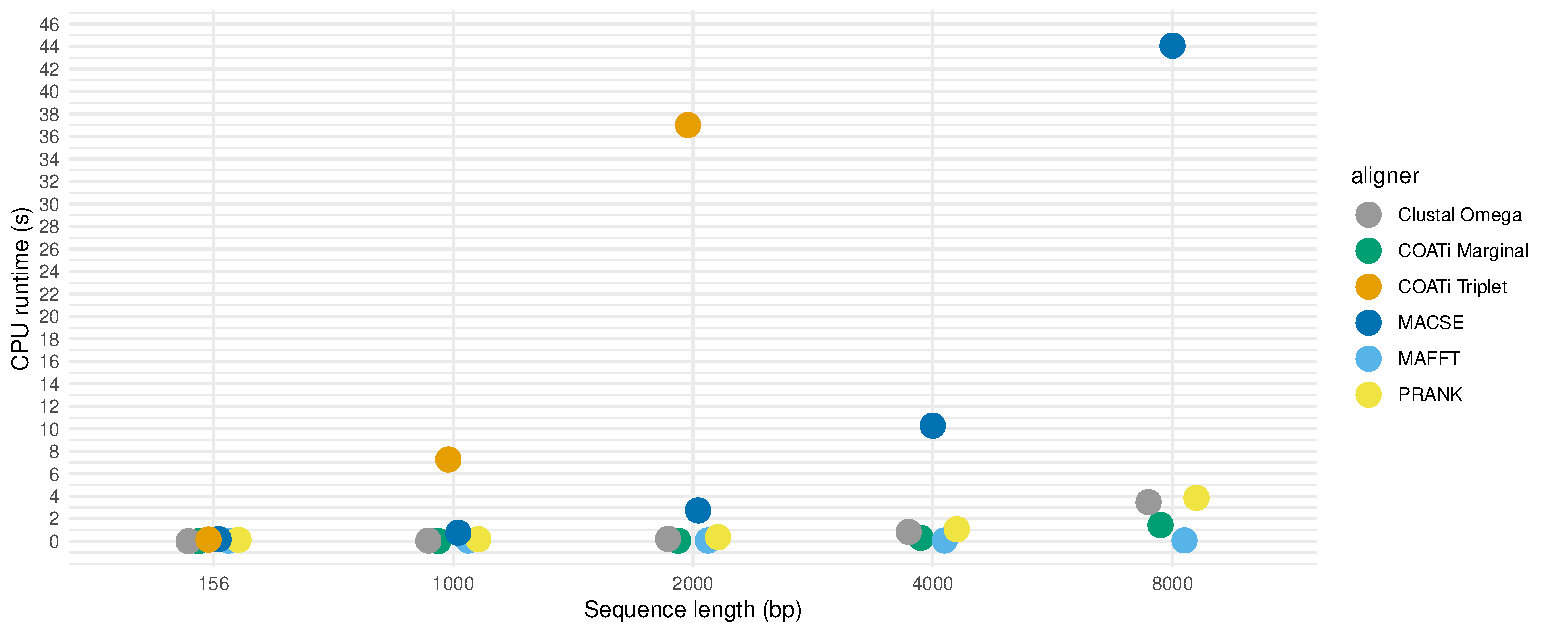
\includegraphics[width = \textwidth]{chapter3/figures/results/runtime_aligners.pdf}
    \caption[Runtime Comparison of Aligners]{Execution time of benchmark in seconds of Clustal$\Omega$, COATi triplet and marginal model, MACSE, MAFFT, and PRANK aligning pairwise sequences of different lengths. COATi triplet, implemented using FSTs, suffers from a costly runtime compared to other aligners. In comparison, COATi marginal solves the issue and can perform similarly to Clustal $\Omega$, MAFFT, and PRANK and better than MACSE. This was run on an 11\textsuperscript{th} generation Intel chip with a single core.}
    \label{fig:alns-benchmark}
\end{figure}

The results (Fig.~\ref{fig:alns-benchmark}) show the execution time of the aligners with different sequence lengths. The runtime for the triplet model (orange) rapidly grows and can become a limitation when sequences exceed a thousand base pairs. Notably, the COATi marginal (green) is comparable to popular tools and considerably faster than MACSE for longer sequence pairs. Both \DIFdelbegin \DIFdel{marginal-max and marginal-sum }\DIFdelend \DIFaddbegin \DIFadd{modal and marginal }\DIFaddend models are reported under COATi marginal because, despite their different definitions, their alignment algorithms are identical, therefore having matching execution times.

\DIFdelbegin \subsection{\DIFdel{Alignment Accuracy}} %DIFAUXCMD
\addtocounter{subsection}{-1}%DIFAUXCMD
%DIF < %%%%%%%%%%%%%%%%%%%%%%%%%%%%%%%%%%%%%%%%%%%%%%%
%DIFDELCMD < 

%DIFDELCMD < %%%
\subsubsection{\DIFdel{MG94}}
%DIFAUXCMD
\addtocounter{subsubsection}{-1}%DIFAUXCMD
%DIFDELCMD < 

%DIFDELCMD < %%%
\DIFdel{The triplet MG94 model consistently outperformed the marginal MG94 models across all datasets (Fig.~\ref{fig:results_tri_mar_mg}). At the lowest branch length of $0.2$, the average alignment error among all three models is similar. However, an evident order emerges, with the triplet-mg model outperforming marginal-mg-sum, which, in turn, achieved a smaller $d_{seq}$ than marginal-mg-max. As the number of expected substitutions increases, the $d_{dseq}$ for the marginal-mg-sum model consistently remains close to that of the triplet model, although the latter outperforms the former across all branch lengths. In contrast, the average alignment error for the marginal-mg-max model diverges further from the other models, spiking when, on average, we expect every site to have undergone a mutation (branch length of 1), with a $d_{seq}$ more than twofold its previous value.
}%DIFDELCMD < 

%DIFDELCMD < \begin{figure}[!ht]
%DIFDELCMD < \centering
%DIFDELCMD < 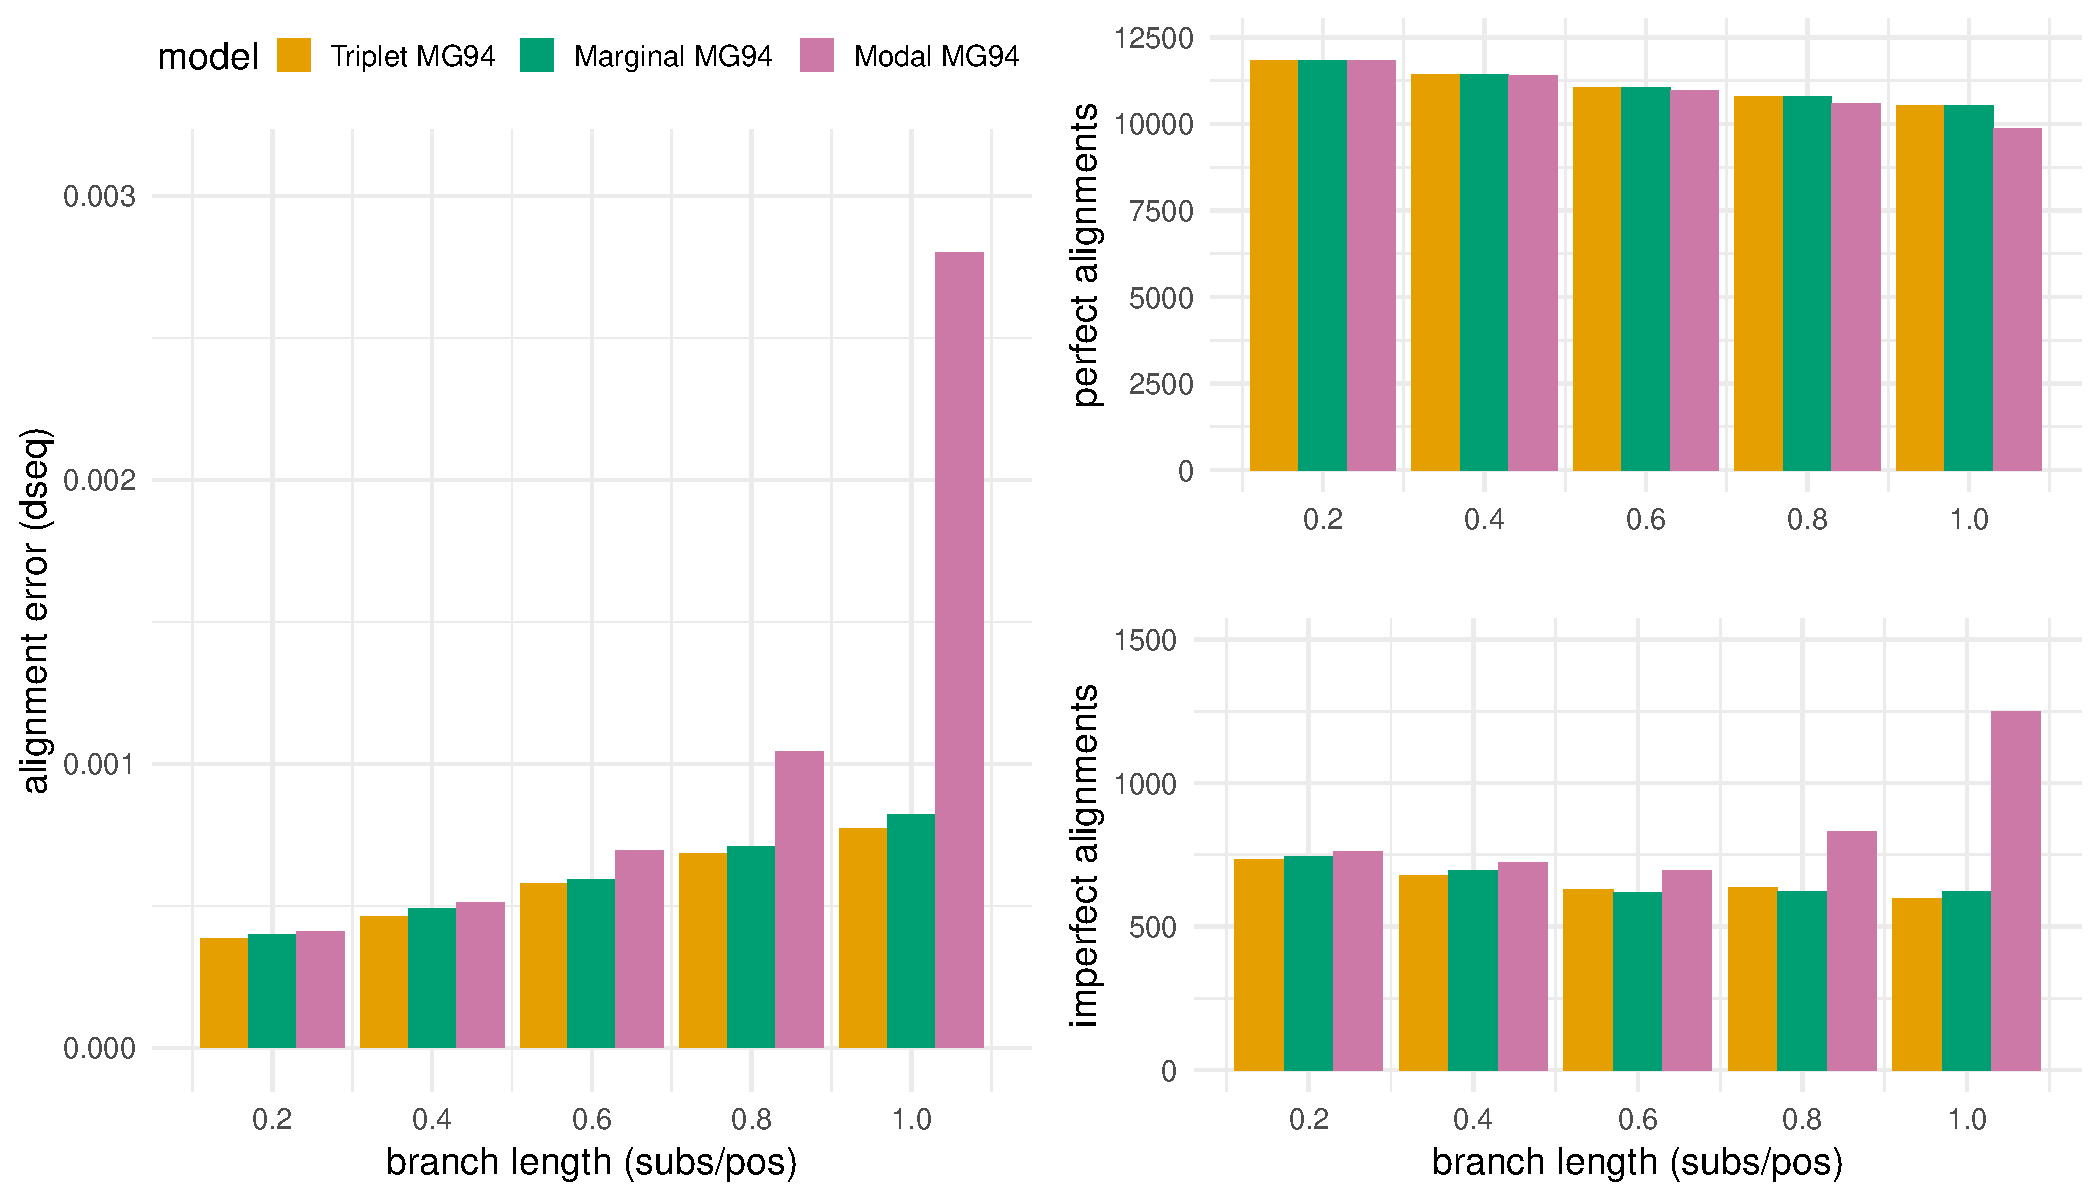
\includegraphics[width=\linewidth]{chapter3/figures/results/results_marginal_triplet_mg.pdf}
%DIFDELCMD <  \vspace{1mm}
%DIFDELCMD <  %%%
%DIFDELCMD < \caption[Alignment Accuracy of the Triplet and Marginal MG94 Models]{%
{%DIFAUXCMD
\DIFdelFL{The triplet-mg model generates better alignments across all branch lengths. Results of triplet-mg, marginal-mg-max, and marginal-mg-sum COATi models in aligning 13,758 simulated sequence pairs. Best alignments have the lowest $d_{seq}$, perfect alignments have the same score as the true alignment or a zero $d_{seq}$, and imperfect alignments have a different score than true alignments when at least one model found a perfect alignment.}}
 %DIFAUXCMD
%DIFDELCMD < \label{fig:results_tri_mar_mg}
%DIFDELCMD < \end{figure}
%DIFDELCMD < 

%DIFDELCMD < %%%
\DIFdel{The number of perfect alignments between the marginal-mg-sum and triplet-mg model remains consistent across all branch lengths. In contrast, the marginal-mg-max starts producing an equal number of perfect alignments for a branch length of $0.2$, but this number declines as branch lengths increase. A similar trend is observed in the count of imperfect alignments, with the marginal-mg-max model producing more imperfect alignments, particularly spiking at branch lengths of $0.8$ and $1.0$. In this section, the remaining models performed similarly, with the marginal-mg-sum model outperforming the triplet-mg model with branch lengths $0.6$ and $0.8$, with the reverse outcome for branch lengths $0.2$, $0.4$, and $1.0$. Note that the count of perfect and imperfect alignments decreases along the x-axis, as alignments not perfectly retrieved by either method are excluded from the results.
}%DIFDELCMD < 

%DIFDELCMD < %%%
\subsubsection{\DIFdel{ECM}}
%DIFAUXCMD
\addtocounter{subsubsection}{-1}%DIFAUXCMD
%DIFDELCMD < 

%DIFDELCMD < %%%
\DIFdel{As expected, the triplet-ecm model outperforms the marginal models across all branch lengths in all metrics (Fig.~\ref{fig:results_tri_mar_ecm}). The trend observed in the MG94 results is intensified in the ECM results. The $d_{seq}$ values for the triplet-ecm and marginal-ecm-sum models are comparable to their MG94 counterparts, albeit with a slightly larger difference between them. This pattern is also evident in the number of perfect and imperfect alignments, where the triplet-ecm model significantly outperforms the marginal models. However, the marginal-ecm-sum model provides a better approximation. In contrast, the marginal-ecm-max model underperforms with a $d_{seq}$ two orders of magnitude larger than its MG94 counterpart for a branch length of 1. The model struggles with short branch lengths, and its performance declines as the number of expected substitutions per site increases. I have truncated the $d_{seq}$ values at $0.05$ to ensure a proper display of the results for the triplet-ecm and marginal-ecm-sum. A comprehensive results table can be found in the appendix (Table \ref{table:results-ecm}).
}%DIFDELCMD < 

%DIFDELCMD < \begin{figure}[!ht]
%DIFDELCMD < \centering
%DIFDELCMD < 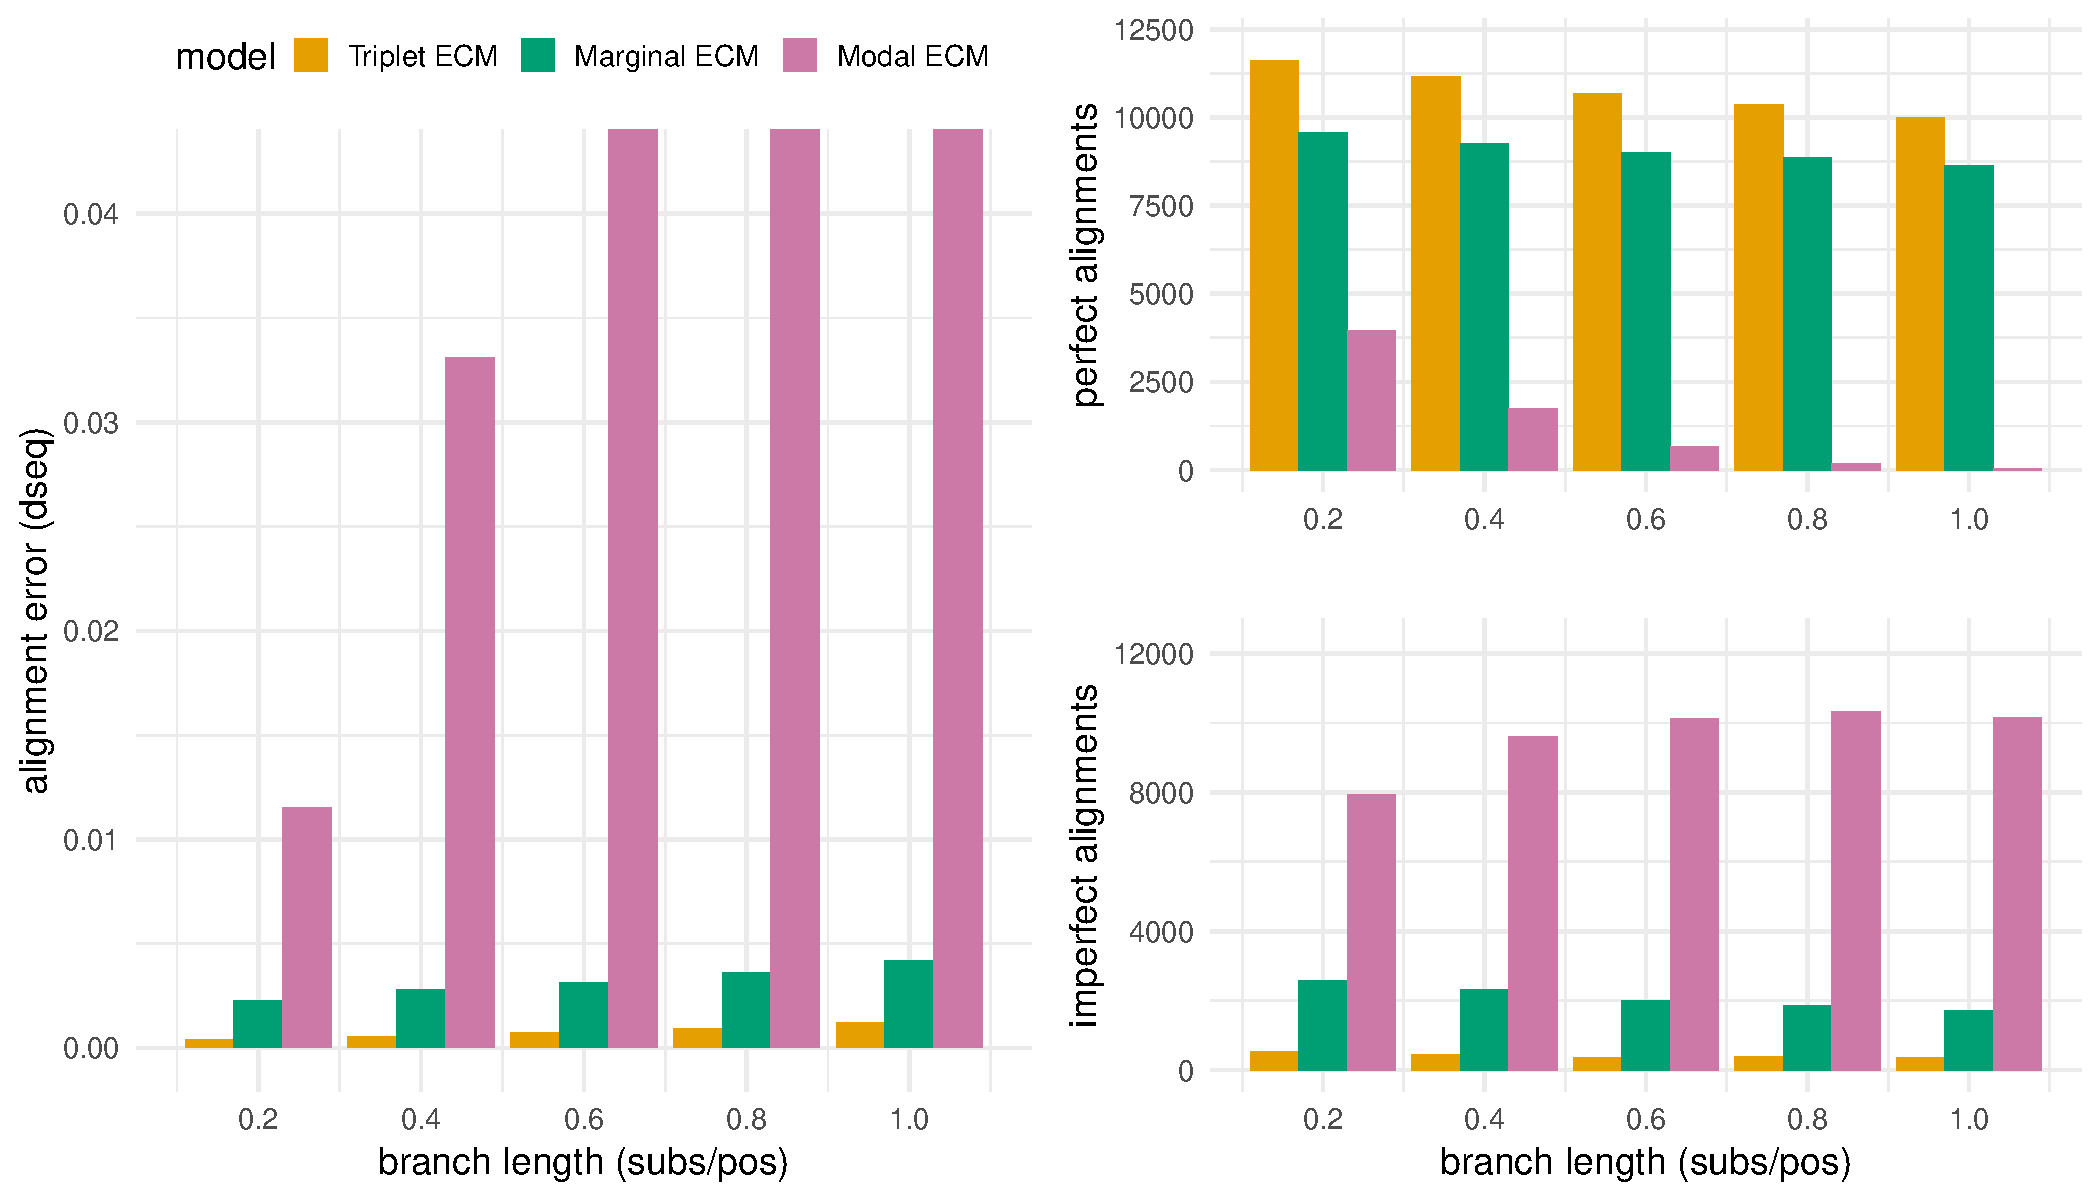
\includegraphics[width=\linewidth]{chapter3/figures/results/results_marginal_triplet_ecm.pdf}
%DIFDELCMD <  \vspace{1mm}
%DIFDELCMD <  %%%
%DIFDELCMD < \caption[Alignment Accuracy of the Triplet and Marginal ECM Models]{%
{%DIFAUXCMD
\DIFdelFL{The triplet-ecm model generates better alignments across all branch lengths. Results of triplet-ecm, marginal-ecm-max, and marginal-ecm-sum COATi models in aligning 13,758 simulated sequence pairs. Best alignments have the lowest $d_{seq}$, perfect alignments have the same score as the true alignment or a zero $d_{seq}$, and imperfect alignments have a different score than true alignments when at least one model found a perfect alignment.}}
 %DIFAUXCMD
%DIFDELCMD < \label{fig:results_tri_mar_ecm}
%DIFDELCMD < \end{figure}
%DIFDELCMD < 

%DIFDELCMD < %%%
\subsection{\DIFdel{Gaps Statistics}} %DIFAUXCMD
\addtocounter{subsection}{-1}%DIFAUXCMD
%DIF < %%%%%%%%%%%%%%%%%%%%%%%%%%%%%%%%%%%%%%%%%%%%%%%%%%%%%%%%%%%%%
%DIFDELCMD < 

%DIFDELCMD < %%%
\DIFdel{Gap statistics can provide valuable insights when comparing alignment models across varying evolutionary distances, as they reveal how the likelihood of substitution relative to indel probabilities changes. Notably, for both the MG94 and ECM models, the total number of gaps and their cumulative length remains constant for both the triplet and marginal-sum models as branch lengths increase (Fig.~\ref{fig:results_tri_mar_mg_gaps}). In concordance with the previous metrics, the behavior of the marginal-max model takes a divergent path, especially for marginal-ecm-max. While the marginal-mg-max model shows similar values until branch length reaches $0.6$ and is slightly elevated thereafter, the total number and length of gaps for the marginal-ecm-max model are larger for all branch lengths.
}%DIFDELCMD < 

%DIFDELCMD < \begin{figure}[!ht]
%DIFDELCMD < \centering
%DIFDELCMD < 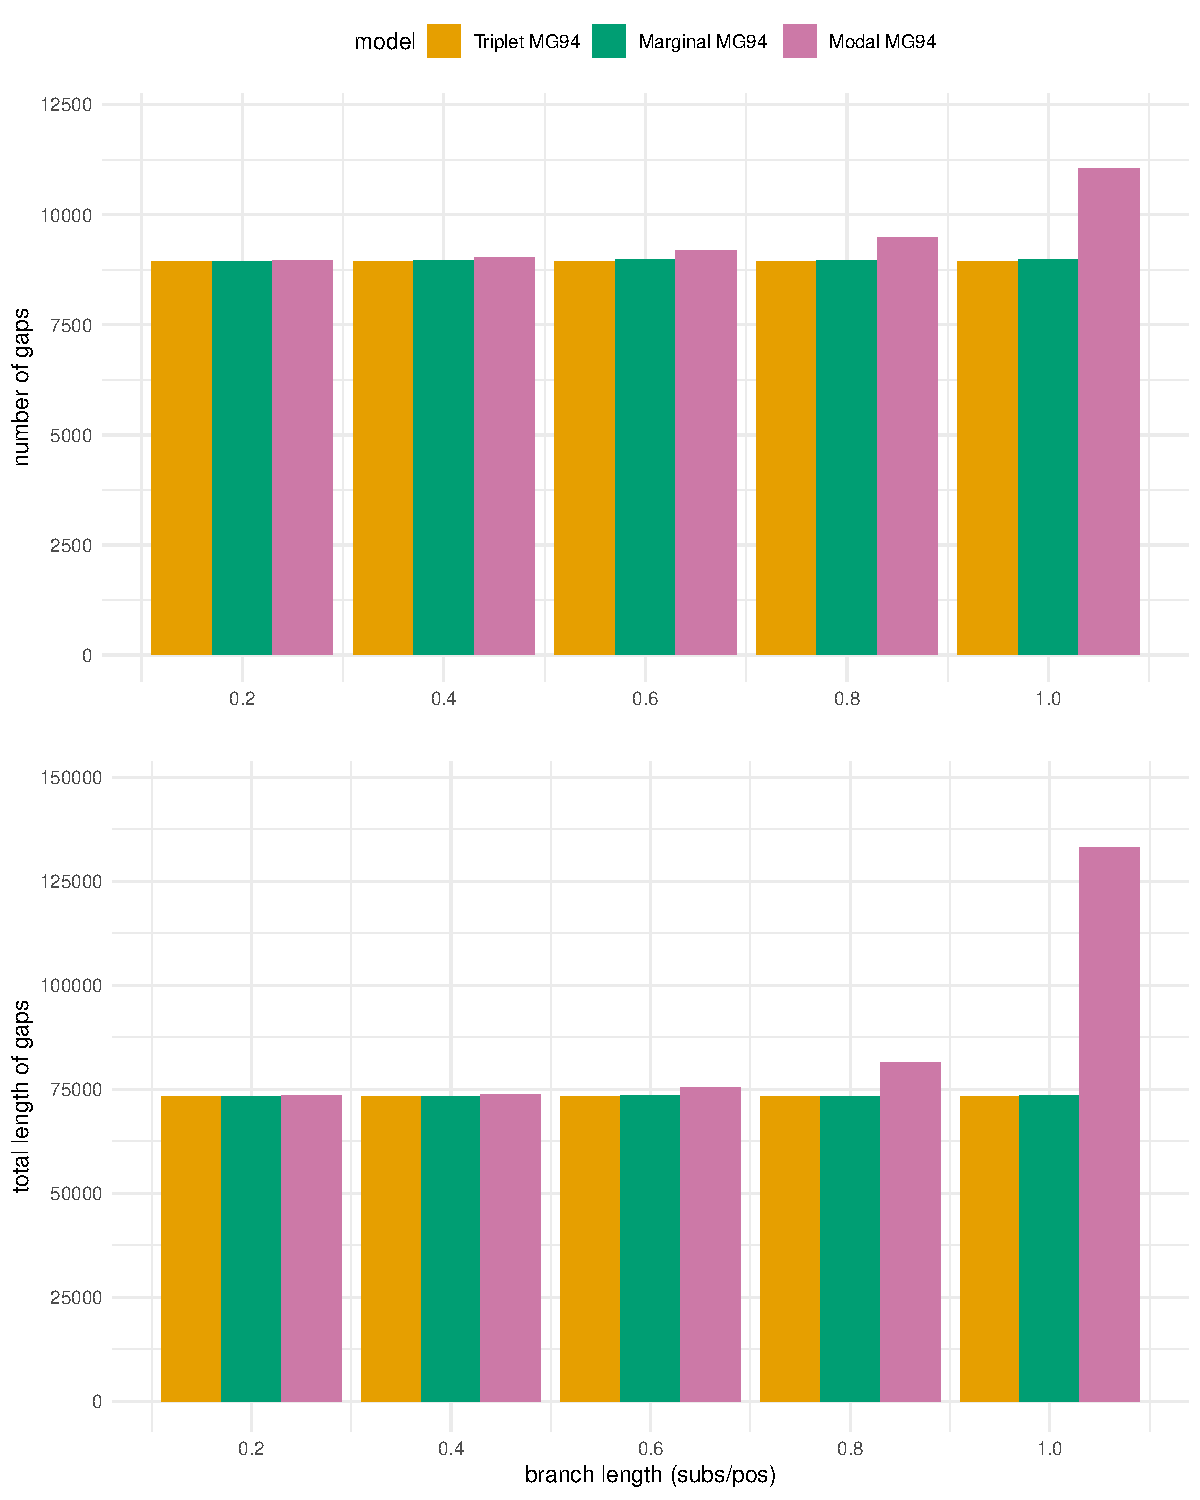
\includegraphics[width = 0.75\linewidth]{chapter3/figures/results/results_marginal_triplet_mg_gaps.pdf}
%DIFDELCMD <  \vspace{1mm}
%DIFDELCMD <  %%%
%DIFDELCMD < \caption[MG94 Dataset Indel Statistics]{%
{%DIFAUXCMD
\DIFdelFL{The number and total length of gaps for triplet-mg and marginal-mg-sum models stay constant as branch lengths increase. On the contrary, the marginal-mg-max model adds more and longer gaps as the evolutionary distance between sequences becomes larger.}}
 %DIFAUXCMD
%DIFDELCMD < \label{fig:results_tri_mar_mg_gaps}
%DIFDELCMD < \end{figure}
%DIFDELCMD < 

%DIFDELCMD < \begin{figure}[!ht]
%DIFDELCMD < \centering
%DIFDELCMD < 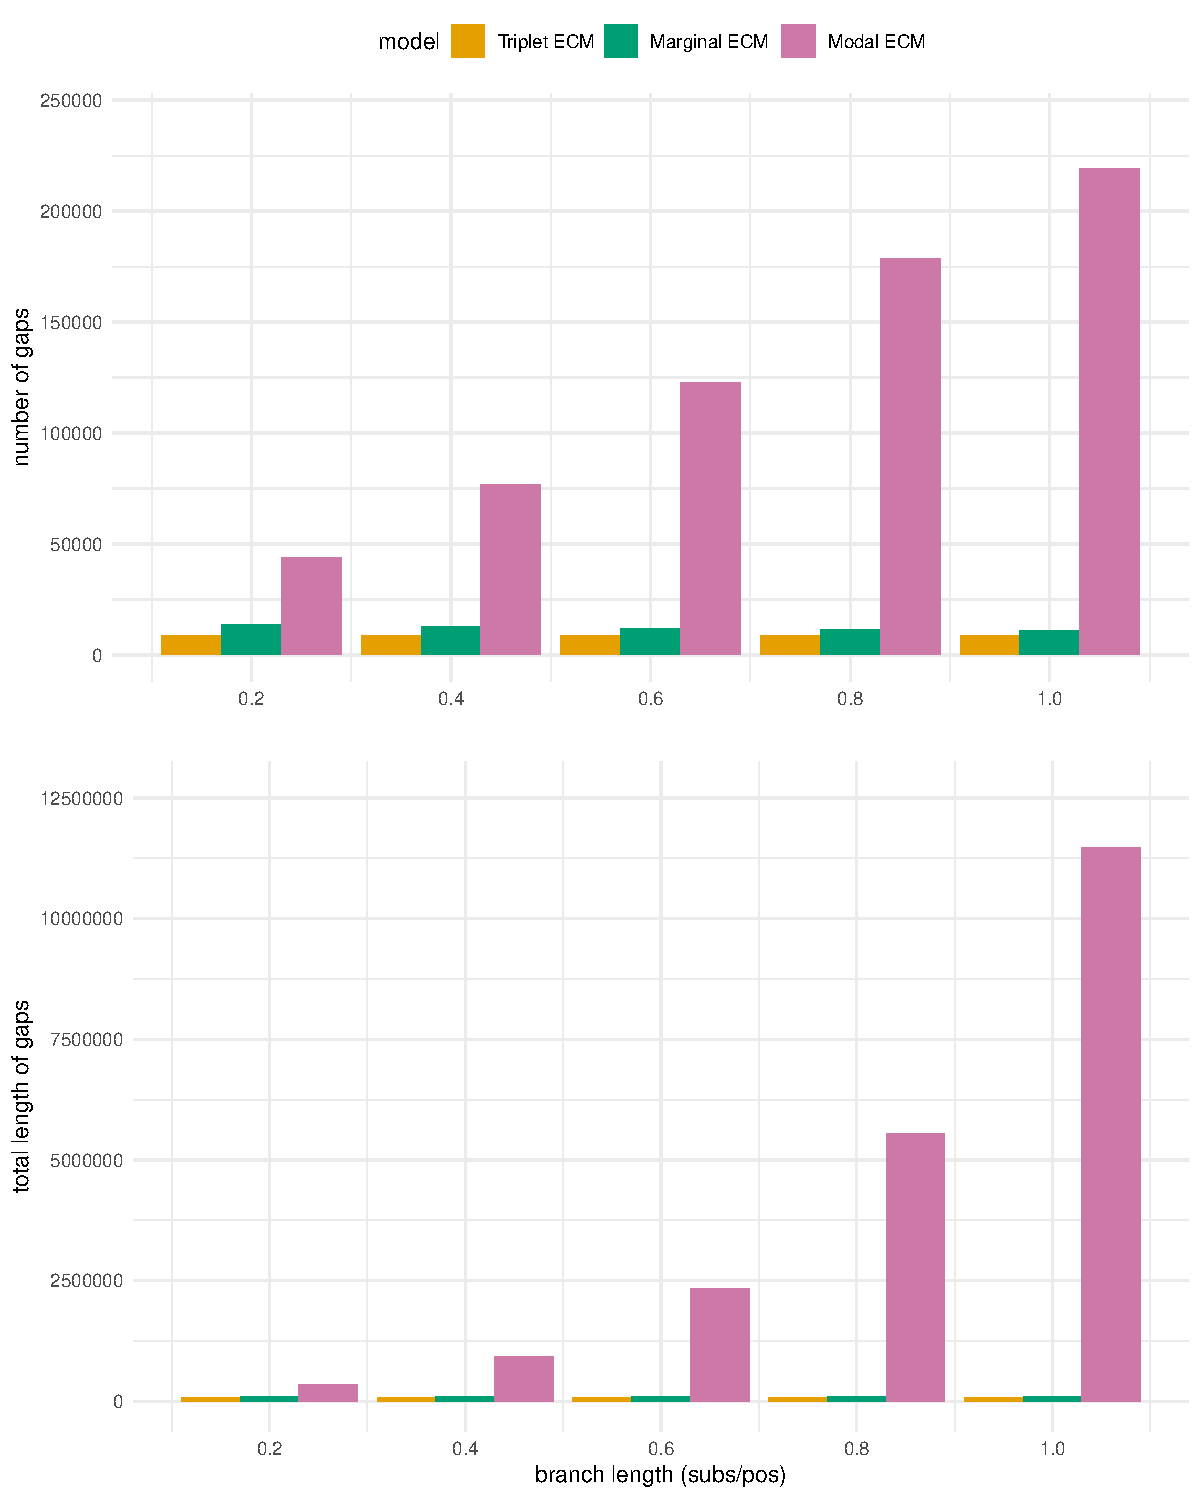
\includegraphics[width = 0.75\linewidth]{chapter3/figures/results/results_marginal_triplet_ecm_gaps.pdf}
%DIFDELCMD <  \vspace{1mm}
%DIFDELCMD <  %%%
%DIFDELCMD < \caption[ECM Dataset Indel Statistics]{%
{%DIFAUXCMD
\DIFdelFL{The number and total length of gaps for triplet-ecm and marginal-ecm-sum models stay constant as branch lengths increase. On the contrary, the marginal-ecm-max model significantly adds more and longer gaps as the evolutionary distance between sequences becomes larger.}}
 %DIFAUXCMD
%DIFDELCMD < \label{fig:results_tri_mar_ecm_gaps}
%DIFDELCMD < \end{figure}
%DIFDELCMD < 

%DIFDELCMD < \clearpage
%DIFDELCMD < 

%DIFDELCMD < %%%
\DIFdelend %%%%%%%%%%%%%%%%%%%%%%%%%%%%%%%%%%%%%%%%%%%%%%%%%%%%%%%%%%%%%%%%%%%%%%%%%%%%%%%%
\section{Discussion}

% \begin{itemize}
%     \item Marginal-max is no bueno, (probably) due to how substitution probabilities change over t.
%     \item Marginal-sum is a good approximation, yet triplet is best (as expected since datasets are simulated using the triplet algorithm).
%     \item Anything else?
% \end{itemize}

While the statistical pairwise sequence aligner COATi can align protein-coding regions in the presence of artifacts with higher accuracy than current methods, the execution time required for sequences longer than a few thousand nucleotides can be a limiting factor. To address this limitation, I developed \DIFdelbegin \DIFdel{a marginal approximation }\DIFdelend \DIFaddbegin \DIFadd{an approximate model }\DIFaddend of the core evolutionary model (triplet) that can be implemented using standard dynamic programming techniques and speeds up the alignment operation to execution times comparable with popular aligners. In this chapter, I have undertaken a comprehensive exploration of the \DIFaddbegin \DIFadd{modal and }\DIFaddend marginal models, providing a detailed description of their definitions and assessing their accuracy in approximating the evolutionary processes of the triplet model.

The evaluation of results across various branch lengths highlights the remarkable fidelity of the \DIFdelbegin \DIFdel{marginal-sum }\DIFdelend \DIFaddbegin \DIFadd{marginal }\DIFaddend model to the triplet model, with similar outcomes in average alignment error and the number of perfect alignments. Conversely, the performance of the \DIFdelbegin \DIFdel{marginal-max }\DIFdelend \DIFaddbegin \DIFadd{modal }\DIFaddend model, while comparable for short branch lengths, gradually diminishes as branch lengths increase. This decline in performance can be attributed to how the substitution probabilities are handled over evolutionary time, as per the definition of the model. Consequently, I recommend employing the triplet model for achieving the highest accuracy, especially when sequence lengths and computational resources permit. However, in cases where these factors pose a limitation, the \DIFdelbegin \DIFdel{marginal-sum }\DIFdelend \DIFaddbegin \DIFadd{marginal }\DIFaddend model, accompanied by its dynamic programming alignment approach, is a robust alternative.

% LIMITATIONS

% The models in COATi, as is inherent to all models in biology, are an approximation of the evolutionary processes that take place in nature and have limitations. An assumption in the pairwise aligner is the imposition of directionality in evolution. Specifically, one sequence is treated as the ancestor, while the other assumes the role of the descendant. This assumption stems from the premise that the ancestor sequence is of higher quality, which the model leverages to preserve the reading frame and eliminate potential artifacts in the descendant sequence. 
% In addition, while the triplet substitution model in COATi is time reversible, the marginal approximations and the indel model are not.

% % We think this is one of the features that helps COATi outperform other tools 
% Although this characteristic of the model benefits the accuracy of the alignment, as it filters out errors in sequencing and annotation, it introduces a bias. I propose two potential solutions to mitigate the impact of the ancestor-descendant assumption. A straightforward approach that can be applied to large datasets, where the goal is to compute summary statistics, is to assign the ancestor role to either sequence. Alternatively, a more robust solution is to modify the alignment algorithm to conduct two Viterbi runs, using a different sequence as the ancestor each time and finding the path that maximizes both Viterbi tracebacks.

\DIFaddbegin \DIFadd{The analysis described in this chapter can be further improved by adjusting gap opening rates in the sequence evolution simulator according to changes in branch length. The algorithm used in this chapter has a fixed gap opening parameter $g$ that does not scale with branch length. In addition, the simulation algorithm should implement different rates for insertion and deletion events, aligning more closely with the prevalent patterns often observed in biological data \mbox{%DIFAUXCMD
\citep{zhang2003patterns,de1981causes}}\hspace{0pt}%DIFAUXCMD
.
}

\DIFaddend Future work includes developing an algorithm that can search alignment space to improve the initial multiple-sequence alignment that COATi can currently produce. This will allow COATi to improve the results on the accurate alignment inference of protein-coding regions in the presence of artifacts, a pressing issue in modern computational biology.

%%%%%%%%%%%%%%%%%%%%%%%%%%%%%%%%%%%%%%%%%%%%%%%%%%%%%%%%%%%%%%%%%%%%%%%%%%%%%%%%
% coati sample??
% coati msa?? \newpage 
 \newpage \chapter{AlnDotPlot: Visual Representation and Analysis of Pairwise Alignments}  \label{ch:alndotplot}

\section{Introduction}
% Nature of the problem
% * sequence alignment is hard
% * There's been improvement because it's an important problem
% * yet comparison between sequence alignments has not seen any major developments - describe current tools
\DIFdelbegin %DIFDELCMD < 

%DIFDELCMD < %%%
\DIFdelend The analysis of biological sequences is the \DIFdelbegin \DIFdel{reconstruction }\DIFdelend \DIFaddbegin \DIFadd{inference }\DIFaddend of unique and unobservable evolutionary events at the DNA level \DIFdelbegin \DIFdel{that cannot be either observed or quantified and must, therefore, be inferred }\DIFdelend \citep{morrison_MSA_2018}. Alignment inference is an essential step required to address questions across multiple branches of biology, including molecular biology, microbiology, and ecology. The field has seen substantial progress since modern sequence alignment began with the computer-adaptable algorithm of Needleman and Wunsch \citeyearpar{Needleman1970}, replacing the arduous manual arrangement of residues as the default method for sequence alignment.

% Current knowledge and limitations
% * tools and methods to evaluate sequence alignment are almost as important as the alignment algorithms themselves
% * current options to evaluate the accuracy of alignments are these, with these limitations
% * probably a couple of paragraphs grouping tools by type

The development of sequence alignment methods has experienced a continuous effort to improve both their accuracy and speed. The quality of sequence alignments directly impacts the reliability of downstream analyses, and thus, alignment evaluation plays a pivotal role in quality control. Existing evaluation methods can be divided into metrics and scores that summarize similarities between alignments and tools that quantify the uncertainty associated with each column of an alignment. A limitation of these methods is that they can compare a summary metric between two alignments or provide site information about an alignment, but cannot combine both approaches. While aligners typically report a single best result using an evolutionary or scoring model, equally optimal (equivalent) alignments often exist and are rarely reported. However, equivalent alignments and suboptimal alternatives are common in sampling and multiple sequence refinement. Being able to perform a thorough comparison between such alignments can be very valuable for understanding how the underlying biological models work. This can also lead to more detailed comparisons of different methods in validating sequence aligners, improve the algorithms that search for suboptimal alignments in multiple sequence refinement, and better assess sampling results.

\subsection{Alignment Accuracy}

% explain B - metrics that summarize alignment similarities - SOP, TC, d_{seq}
Popular alignment similarity scores include sum-of-pairs (SP) and total column score (TC). SP is the percentage of correctly aligned residue pairs in an alignment, which measures how well pairs of sequences are aligned, while TC is the percentage of correctly aligned columns in an alignment, testing the ability to align all sequences correctly \citep{thompson2005balibase}. In the case of pairwise alignment, both metrics are identical. A more informative set of metrics that consider indels and the evolutionary history of events in a phylogenetic tree was put forth by Blackburne and Whelan \citeyearpar{metrics_blackburne_whelan_2011}. These metrics range from zero to one and can be interpreted as the probability that a randomly selected residue will be aligned to a different location against a sequence that does not contain such residue. Notably, similarity and distance metrics are easily scalable to compare results over large datasets. However, they struggle to find specific portions where alignments diverge and what are their differences.

% explain A - tools that quantify position uncertainty - GUIDANCE, T-COFFEE, MUMSA
Tools \DIFaddbegin \DIFadd{and methods }\DIFaddend that quantify alignment uncertainty include \DIFaddbegin \DIFadd{Heat or Tails \mbox{%DIFAUXCMD
\citep{landan2007heads}}\hspace{0pt}%DIFAUXCMD
, a method that considers the probability distribution of possible placements for each sequence within a multiple sequence alignment; }\DIFaddend GUIDANCE \citep{penn2010guidance}, which uses bootstrap algorithms\DIFdelbegin \DIFdel{, }\DIFdelend \DIFaddbegin \DIFadd{; GUIDANCE 2 \mbox{%DIFAUXCMD
\citep{sela2015guidance2}}\hspace{0pt}%DIFAUXCMD
, which combines three sources of uncertainty: co-optimal solutions, guide tree instability, and opening gap penalty; }\DIFaddend ZORRO \citep{wu2012zorro}, based on hidden Markov models\DIFdelbegin \DIFdel{, }\DIFdelend \DIFaddbegin \DIFadd{; }\DIFaddend and MUMSA \citep{lassmann2005mumsa}, which calculates the portion of identically aligned regions\DIFdelbegin \DIFdel{. These software packages }\DIFdelend \DIFaddbegin \DIFadd{; and posterior decoding, a popular method used in the context of Markov models that calculates the probability of each state in the alignment path and is particularly useful when many different paths have almost the same probability as the most likely one. These methods }\DIFaddend provide information about the reliability of each column in an alignment and identify uncertain sections, allowing researchers to remove them to prevent errors that may bias downstream analysis. While these metrics can help improve the quality of genomic pipeline results, they are also limited to analyzing one alignment at a time.

\subsection{Alignment Visualization}

A common feature shared among the alignment uncertainty applications described above is their display of confidence scores and the alignment in matrix form (Fig.~\ref{fig:msa-example}). This format of alignment visualization provides a representation of an alignment, where residues are typically colored by type and are supported by numerous software packages \DIFdelbegin \DIFdel{(e.g., \mbox{%DIFAUXCMD
\citealp{zhou2022ggmsa}}\hspace{0pt}%DIFAUXCMD
) }\DIFdelend and web-based tools (e.g., \DIFaddbegin \DIFadd{\mbox{%DIFAUXCMD
\citealp{zhou2022ggmsa}}\hspace{0pt}%DIFAUXCMD
; }\DIFaddend \citealp{yachdav2016msaviewer}). A matrix representation of an alignment displays two or more aligned sequences as rows, with each column representing a site. However, while this format is intuitive, it does not allow comparing two or more alignments.

\begin{figure}[!ht]
    \centering
    % \resizebox{0.9\textwidth}{!}{
    \definecolor{colorY}{RGB}{255,255,51}   % YELLOW
\definecolor{colorG}{RGB}{77,175,74}    % GREEN
\definecolor{colorB}{RGB}{55,126,184}   % BLUE
\definecolor{colorR}{RGB}{228,26,28}    % RED
\definecolor{colorGy}{RGB}{153,153,153} % GRAY
\DIFaddbeginFL \definecolor{colorP}{RGB}{152,78,163}   %DIF >  PURPLE
\DIFaddendFL 

\DIFdelbeginFL %DIFDELCMD < \begin{tikzpicture}[node distance=1mm,font=\footnotesize]
%DIFDELCMD < \tikzstyle{aln}=[matrix of nodes, nodes in empty cells,fill=colorGy!20]
%DIFDELCMD < \newcommand{\A}{\textcolor{colorY}{\textbf{A}}}
%DIFDELCMD < \newcommand{\C}{\textcolor{colorG}{\textbf{C}}}
%DIFDELCMD < \newcommand{\G}{\textcolor{colorB}{\textbf{G}}}
%DIFDELCMD < \newcommand{\T}{\textcolor{colorR}{\textbf{T}}}
%DIFDELCMD < 

%DIFDELCMD < \matrix (msa)[aln] {
%DIFDELCMD < \C\A\T & \A\A\G & \C\G\G & \T\C\G & \G\A\C & \verb|---|\\
%DIFDELCMD < \C\A\G & \C\A\G & \C\G\G & \T\C\G & \G\A\C & \A\C\G\\
%DIFDELCMD < \C\A\T & \C\A\G & \C\G\G & \T\C\verb|-| & \verb|--|\C & \A\C\A\\
%DIFDELCMD < \C\A\T & \C\A\G & \C\C\G & \T\C\G & \G\A\C & \A\C\G\\
%DIFDELCMD < };
%DIFDELCMD < \end{tikzpicture}
%DIFDELCMD <     %%%
\DIFdelendFL \DIFaddbeginFL \begin{tikzpicture}[node distance=1mm,font=\footnotesize]
\tikzstyle{aln}=[matrix of nodes, nodes in empty cells,fill=colorGy!20]
\newcommand{\A}{\textcolor{colorP}{\textbf{A}}}
\newcommand{\C}{\textcolor{colorG}{\textbf{C}}}
\newcommand{\G}{\textcolor{colorB}{\textbf{G}}}
\newcommand{\T}{\textcolor{colorY}{\textbf{T}}}

\matrix (msa)[aln] {
\C\A\T & \A\A\G & \C\G\G & \T\C\G & \G\A\C & {\color{blue}%DIFAUXCMD
\verb|---|%
}%DIFAUXCMD
\\
\C\A\G & \C\A\G & \C\G\G & \T\C\G & \G\A\C & \A\C\G\\
\C\A\T & \C\A\G & \C\G\G & \T\C{\color{blue}%DIFAUXCMD
\verb|-| %
}%DIFAUXCMD
& {\color{blue}%DIFAUXCMD
\verb|--|%
}%DIFAUXCMD
\C & \A\C\A\\
\C\A\T & \C\A\G & \C\C\G & \T\C\G & \G\A\C & \A\C\G\\
};
\end{tikzpicture}
    \DIFaddendFL \caption[Multiple Sequence Alignment Plot]{Example of a DNA multiple sequence alignment visualization in matrix form. Every row corresponds to a sequence and every column is a position in the alignment. Nucleotides are colored by type and gaps are shown in black.}
    \label{fig:msa-example}
\end{figure}

% An additional and perhaps less used visualization method is dot plots.
% Describe dot plots, including what they are and represent, their use cases, and their limitations.
Dot plots are an additional visual representation tool used to compare two sequences that facilitate the identification of similarities, differences, and underlying patterns, introduced by Gibbs and McIntyre \citeyearpar{gibbs1970dotplot}. They consist of a matrix where one sequence is displayed on the x-axis, left to right, and the other on the y-axis, top to bottom, and using dots indicate matching residues between the sequences. Conversely, mismatching nucleotides are left blank. Note that gap symbols are typically not considered in dot plots as they evaluate unaligned sequences.

In biological sequence analysis, dot plots are suitable for identifying regions of similarity between sequences, evidenced by diagonal lines of dots that run left to right and top to bottom. The length and pattern of these contiguous dots provide insight into the nature and extent of the similarity. In addition, dot plots are used to identify specific biological events, including repeated regions, tandem repeats, palindromic regions, and microsatellite patterns (Fig. \ref{fig:dotplot-patterns}). This illustrates that dot plots are a simple and versatile tool for comparing pairs of unaligned sequences.

\begin{figure}[!ht]
    \centering
    \DIFdelbeginFL %DIFDELCMD < 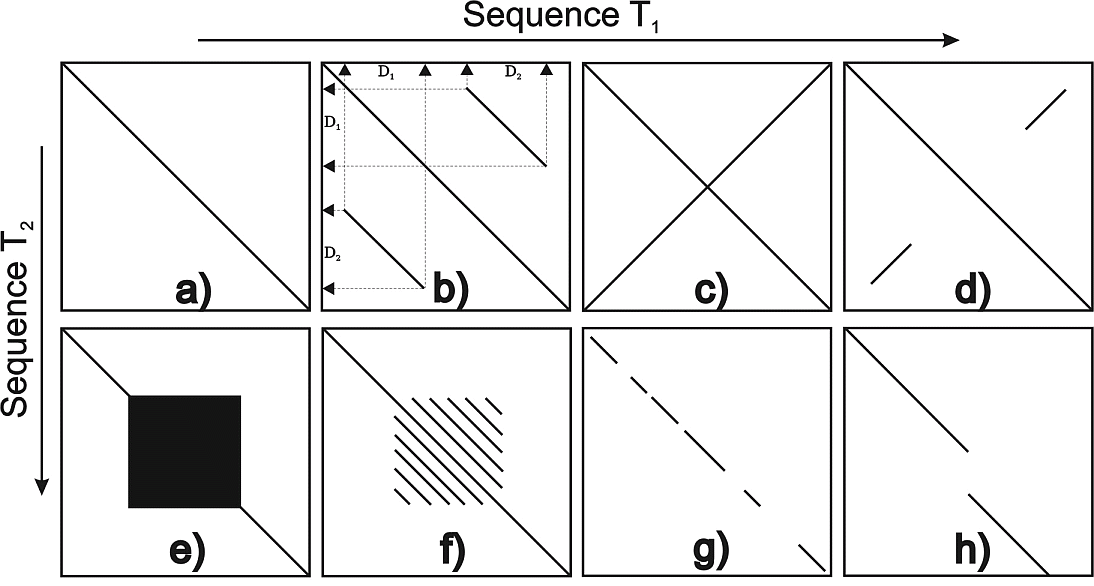
\includegraphics[width = \textwidth]{chapter4/figures/dotplot-patterns.png}
%DIFDELCMD <     %%%
\DIFdelendFL \DIFaddbeginFL \scalebox{1}{\begin{tikzpicture}
    % First square
    \draw (0,0) rectangle (4,4);
    \draw (0,4) -- (4,0);
    \node (a) at (0.3,0.3) {a)};

    % Second square
    \draw (5,0) rectangle (9,4);
    \draw (5,4) -- (9,0);
    \draw (7,3) -- (8,2);
    \draw (6,2) -- (7,1);
    \node (b) at (5.3, 0.3) {b)};

    % Third square
    \draw (0,-1) rectangle (4,-5);
    \draw[dashed] (0,-1) -- (4,-5);
    \node (c) at (0.3, -4.7) {c)};

    % Fourth square
    \draw (5,-1) rectangle (9,-5);
    \draw (5,-1) -- (6.5,-2.5);
    \draw (6.5,-3.5) -- (8,-5);
    \node (d) at (5.3, -4.7) {d)};

    % Sequences
    \draw[->] (-0.5,3) -- (-0.5,-4);
    \draw[->] (1,4.5) -- (8,4.5);
    \node (T1) at (4.5,5) {Sequence T$_1$};
    \node[rotate=90] (T3) at (-1,-0.5) {Sequence T$_2$};
\end{tikzpicture}}
    %DIF >  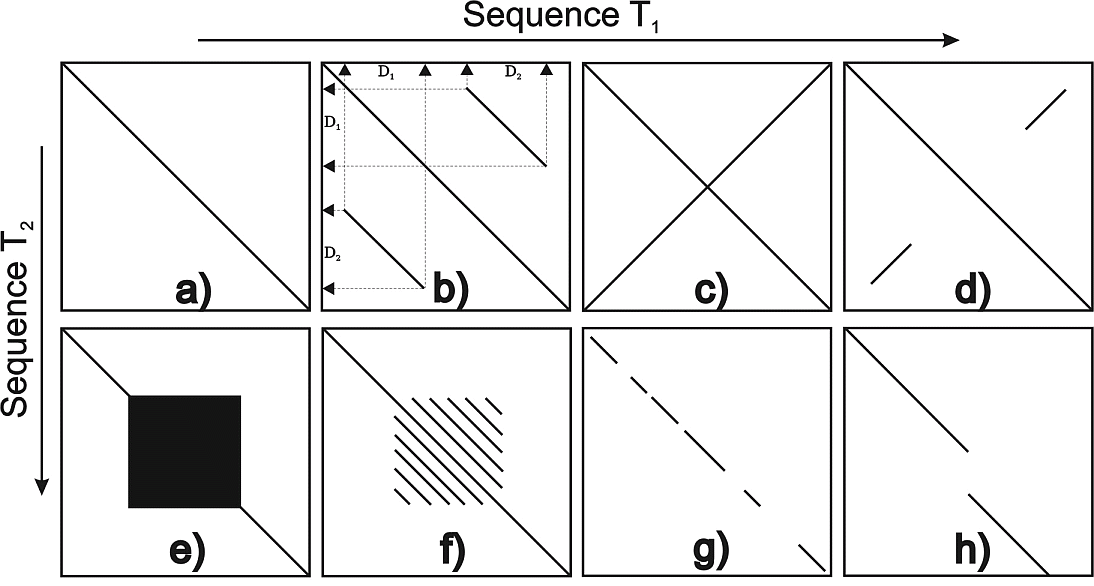
\includegraphics[width = \textwidth]{chapter4/figures/dotplot-patterns.png}
    \DIFaddendFL \caption[Overview of patterns found in dot plots]{\DIFdelbeginFL \emph{\DIFdelFL{Source}}%DIFAUXCMD
\DIFdelFL{: \mbox{%DIFAUXCMD
\citealp{schulz2008code10}}\hspace{0pt}%DIFAUXCMD
}\DIFdelendFL . Overview of characteristic patterns in dot plots.
    \textbf{a)} A continuous main diagonal shows perfect similarity.
    \textbf{b)} Parallels to the main diagonal indicate repeated regions on different parts of the sequences.
    \textbf{c)} \DIFdelbeginFL \DIFdelFL{Lines perpendicular to the main diagonal indicate palindromic areas.
    }\textbf{\DIFdelFL{d)}} %DIFAUXCMD
\DIFdelFL{Partially palindromic sequence, frequently found for transposable elements.
    }\textbf{\DIFdelFL{e)}} %DIFAUXCMD
\DIFdelFL{Bold blocks on the main diagonal indicate repetition of the same symbols in both sequences, called microsatellite repeats.
    }\textbf{\DIFdelFL{f)}} %DIFAUXCMD
\DIFdelFL{Parallel lines indicate tandem repeats of a larger motif in both sequences, called minisatellite patterns.
    }\textbf{\DIFdelFL{g)}} %DIFAUXCMD
\DIFdelendFL When the diagonal is a discontinuous line this indicates that the sequences \DIFdelbeginFL \DIFdelFL{T1 }\DIFdelendFL \DIFaddbeginFL \DIFaddFL{T$_1$ }\DIFaddendFL and \DIFdelbeginFL \DIFdelFL{T2 }\DIFdelendFL \DIFaddbeginFL \DIFaddFL{T$_2$ }\DIFaddendFL share a common ancestor.
    \DIFdelbeginFL \textbf{\DIFdelFL{h)}} %DIFAUXCMD
\DIFdelendFL \DIFaddbeginFL \textbf{\DIFaddFL{d)}} \DIFaddendFL Partial deletion in sequence T1 or insertion in sequence T2. \DIFaddbeginFL \DIFaddFL{Work modified from \mbox{%DIFAUXCMD
\citealp{schulz2008code10}}\hspace{0pt}%DIFAUXCMD
}\DIFaddendFL }
    \label{fig:dotplot-patterns}
\end{figure}

\subsection{Comparison of Pairwise Alignments}
% Then aims and study relevance - I developed AlnDotPlot to address (some of) these limitations.
% General description and impact.
% Sampling, compare alternative and suboptimal alignments, algo más?

The tools described above provide valuable and scalable algorithms for measuring distance or scoring similarity between alignments and methods for identifying uncertain regions within alignments. However, they cannot provide detailed information about how and where alignments differ. To fill this gap, I have developed AlnDotPlot, a visual tool inspired by traditional dot plots that can compare alternative pairwise alignments and is available as an R package. AlnDotPlot can provide a detailed comparison between a handful of pairwise alignments, identify patterns in hundreds of alignment sampling results, and find short base pair differences among alignments of a few kilobases. This software combines the simple nature of dot plots with features to analyze pairwise sequence alignments.

\section{Implementation}

AlnDotPlot can generate alignment dot plots that compare sets of pairwise alignments. This R package can read in alignments in FASTA format and produce results in PDF and TEX format. Internally, the alignment information is converted into matrices, which are in turn, used to create the dot plots. I use the \textit{tikzDevice} R package to create the final results for its versatility and accuracy \citep{sharpsteen2023tikzdevice}. The following sections describe the different models and their implementation and use cases. AlnDotPlot is available as an R software package at \url{https://www.github.com/jgarciamesa/alndotplot}.

\subsection{From Alignment to Dot Matrix}
% Explain how to go from alignment to dot plot

AlnDotPlot generates different alignment dot plots given a set of pairwise alignments. To generate these figures, the first step is to read in the pairwise alignments. Next, the alignment information must be transformed into a dot matrix, which stores this information in a conventional two-dimensional matrix. Based on the different model designs, I have implemented two types of dot matrices. For the simplest model, a traditional dot plot, the dot matrix records only the positions within the alignments involving substitutions (matches and mismatches).
Given two sequences $s$ and $v$, this dot matrix has dimensions $|s|$ by $|v|$, where each row corresponds to symbols in $s$ and every column to symbols in $v$. Every cell in the matrix represents a symbol from $s$ that matches (or mismatches) with a symbol in $v$. The value in every cell is the count of substitutions between these symbols across all input alignments. Figure \ref{fig:aln2matrix-traditional} showcases a sample alignment and its corresponding traditional dot matrix.

\begin{figure}[!ht]
    \centering
    % \begin{multicols}{3}
    \begin{subfigure}[c]{0.4\textwidth}
        \centering
        \vspace*{-7em}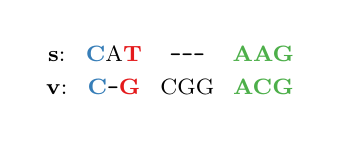
\begin{tikzpicture}[node distance=5mm,font=\footnotesize]
\tikzstyle{aln}=[matrix of nodes, nodes in empty cells]

\definecolor{colorY}{RGB}{255,255,51}   % YELLOW
\definecolor{colorG}{RGB}{77,175,74}    % GREEN
\definecolor{colorB}{RGB}{55,126,184}   % BLUE
\definecolor{colorR}{RGB}{228,26,28}    % RED
\definecolor{colorGy}{RGB}{153,153,153} % GRAY

\newcommand{\B}[1]{\textcolor{colorB}{\textbf{#1}}}
\newcommand{\R}[1]{\textcolor{colorR}{\textbf{#1}}}
\newcommand{\G}[1]{\textcolor{colorG}{\textbf{#1}}}

\matrix (aln1)[aln] {
 % \textbf{Aln 1} & & & &\\
\textbf{s}: & \B{C}A\R{T} & \verb|---| & \G{AAG} &\\
\textbf{v}: & \B{C}\verb|-|\R{G} & CGG & \G{ACG} &\\
};
\end{tikzpicture}
        \vspace*{1.5em}\caption{}
     \end{subfigure}
     \hspace{0.3em}
    \begin{subfigure}[b]{0.4\textwidth}
        \centering
        % Created by tikzDevice version 0.12.4 on 2023-10-07 16:59:03
% !TEX encoding = UTF-8 Unicode
\definecolor{colorY}{RGB}{255,255,51}   % YELLOW
\definecolor{colorG}{RGB}{77,175,74}    % GREEN
\definecolor{colorB}{RGB}{55,126,184}   % BLUE
\definecolor{colorR}{RGB}{228,26,28}    % RED
\definecolor{colorGy}{RGB}{153,153,153} % GRAY
\begin{tikzpicture}[count/.style={color=black, font=\bfseries}]
\draw[very thin, color = gray!50, step = 0.5] (0,0) grid (4.5, 3.5);
\node at (0.25,2.75) {C};
\node at (0.25,2.25) {A};
\node at (0.25,1.75) {T};
\node at (0.25,1.25) {A};
\node at (0.25,0.75) {A};
\node at (0.25,0.25) {G};
\node at (0.75,3.25) {C};
\node at (1.25,3.25) {G};
\node at (1.75,3.25) {C};
\node at (2.25,3.25) {G};
\node at (2.75,3.25) {G};
\node at (3.25,3.25) {A};
\node at (3.75,3.25) {C};
\node at (4.25,3.25) {G};
\node[count] at (0.75, 2.75){\textcolor{colorB}{1}};
\node[count] at (1.25, 1.75){\textcolor{colorR}{1}};
\node[count] at (3.25, 1.25){\textcolor{colorG}{1}};
\node[count] at (3.75, 0.75){\textcolor{colorG}{1}};
\node[count] at (4.25, 0.25){\textcolor{colorG}{1}};
\end{tikzpicture}

        \caption{}
     \end{subfigure}
    %  \hfill
    % \begin{subfigure}[b]{0.3\textwidth}
    %     \centering
    %     % Created by tikzDevice version 0.12.4 on 2023-10-07 16:59:03
% !TEX encoding = UTF-8 Unicode
\definecolor{colorY}{RGB}{255,255,51}   % YELLOW
\definecolor{colorG}{RGB}{77,175,74}    % GREEN
\definecolor{colorB}{RGB}{55,126,184}   % BLUE
\definecolor{colorR}{RGB}{228,26,28}    % RED
\definecolor{colorGy}{RGB}{153,153,153} % GRAY

\begin{tikzpicture}[box/.style={rectangle, fill=gray!50, minimum size=0.5cm}]
\draw[very thin, color = gray!50, step = 0.5] (0,0) grid (4.5, 3.5);
\node at (0.25,2.75) {C};
\node at (0.25,2.25) {A};
\node at (0.25,1.75) {T};
\node at (0.25,1.25) {A};
\node at (0.25,0.75) {A};
\node at (0.25,0.25) {G};
\node at (0.75,3.25) {C};
\node at (1.25,3.25) {G};
\node at (1.75,3.25) {C};
\node at (2.25,3.25) {G};
\node at (2.75,3.25) {G};
\node at (3.25,3.25) {A};
\node at (3.75,3.25) {C};
\node at (4.25,3.25) {G};
\node[box, fill=colorB] at (0.75, 2.75){};
\node[box, fill=colorR] at (1.25, 1.75){};
\node[box, fill=colorG] at (3.25, 1.25){};
\node[box, fill=colorG] at (3.75, 0.75){};
\node[box, fill=colorG] at (4.25, 0.25){};
% \matrix [draw, below right, draw=none] at (current bounding box.north east) {
%         % \node[box, fill=viridis0, scale=0.75] {0\%}; \\
%         \node[box, fill=viridis1, scale=0.75] {00-09\%}; \\
%         \node[box, fill=viridis2, scale=0.75] {10-19\%}; \\
%         \node[box, fill=viridis3, scale=0.75] {20-29\%}; \\
%         \node[box, fill=viridis4, scale=0.75] {30-29\%}; \\
%         \node[box, fill=viridis5, scale=0.75] {\textcolor{white}{40-49\%}}; \\
%         \node[box, fill=viridis6, scale=0.75] {\textcolor{white}{50-59\%}}; \\
%         \node[box, fill=viridis7, scale=0.75] {\textcolor{white}{60-69\%}}; \\
%         \node[box, fill=viridis8, scale=0.75] {\textcolor{white}{70-79\%}}; \\
%         \node[box, fill=viridis9, scale=0.75] {\textcolor{white}{80-89\%}}; \\
%         \node[box, fill=viridis10, scale=0.75] {\textcolor{white}{90-100\%}}; \\
%     };
\end{tikzpicture}

    %     \caption{}
    %  \end{subfigure}

    \caption[Alignment to Traditional Dot Matrix]{Converting a pairwise alignment to a traditional dot matrix. (a) is an alignment of sequences $s$ and $v$, with matches and mismatches (substitutions) colored arbitrarily. (b) is a matrix with the characters in sequence $s$ as rows and the characters in sequence $v$ as columns. The values indicate the count of substitutions between the row and column nucleotides (i.e., the first `C' in both sequences is matched once on the alignment). Note empty cells have a count of zero, omitted here.}
    \label{fig:aln2matrix-traditional}
    % (c) is the dot matrix resulting from the alignment in (a), indicating where the substitutions occur. Here, colors connect the substitutions in the alignment with the cells in the dot matrix.}
\end{figure}

% dot matrix with indels % dot matrix expanded

Expanded dot matrices extend traditional dot matrices, described above, by incorporating indel information, and a similar construction procedure. Given a collection of pairwise alignments between sequences $s$ and $v$, this dot matrix has dimensions $(2\cdot|s|+1)$ by $(2\cdot|v|+1)$, where even rows and columns correspond the symbols in $s$ and $v$ respectively, and odd rows and columns represent gap symbols. Expanding upon the previous dot matrix design, this configuration enables marking insertion and deletion events with clarity. The values within the matrix represent the count of the corresponding row and column symbol pairs found in the alignments. Figure \ref{fig:aln2matrix-expanded} illustrates how an expanded dot matrix is constructed.

\DIFdelbegin %DIFDELCMD < \begin{figure}[!ht]
%DIFDELCMD <     %%%
\DIFdelendFL \DIFaddbeginFL \begin{figure}[!hbt]
    \DIFaddendFL \centering
    \begin{subfigure}[c]{0.2\textwidth}
        \centering
        \vspace*{1em}\hspace*{-2em}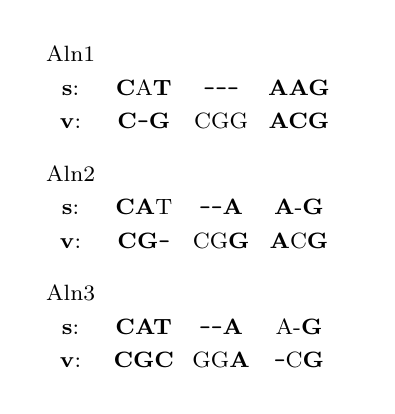
\begin{tikzpicture}[node distance=5mm,font=\footnotesize]
\tikzstyle{aln}=[matrix of nodes, nodes in empty cells]

\definecolor{colorY}{RGB}{255,255,51}   % YELLOW
\definecolor{colorG}{RGB}{77,175,74}    % GREEN
\definecolor{colorB}{RGB}{55,126,184}   % BLUE
\definecolor{colorR}{RGB}{228,26,28}    % RED
\definecolor{colorGy}{RGB}{153,153,153} % GRAY

\newcommand{\N}[1]{\textbf{#1}}

\matrix (aln1) [aln] {
Aln1 & & & &\\
\N{s}: & \N{C}A\N{T} & \verb|---| & \N{AAG} &\\
\N{v}: & \N{C}\verb|-|\bf{G} & CGG & \N{ACG} &\\
% };
% \matrix (aln2) [aln, right=4mm of aln1] {
\\
Aln2 & & & &\\
\N{s}: & \N{CA}T & \verb|--|\N{A} & \N{A}-\N{G} &\\
\N{v}: & \N{CG}\verb|-| & CG\N{G} & \N{A}C\N{G} &\\
% };
% \matrix (aln3) [aln, right=4mm of aln2] {
\\
Aln3 & & & &\\
\N{s}: & \N{CAT} & \verb|--|\N{A} & A-\N{G} &\\
\N{v}: & \N{CGC} & GG\N{A} & \verb|-|C\N{G} &\\
};
\end{tikzpicture}
        \vspace*{1em}\caption{}
     \end{subfigure}
     \hspace{6em}
    \begin{subfigure}[c]{0.5\textwidth}
        \centering
        \resizebox{1.15\textwidth}{!}{% Created by tikzDevice version 0.12.4 on 2023-10-07 18:20:52
% !TEX encoding = UTF-8 Unicode
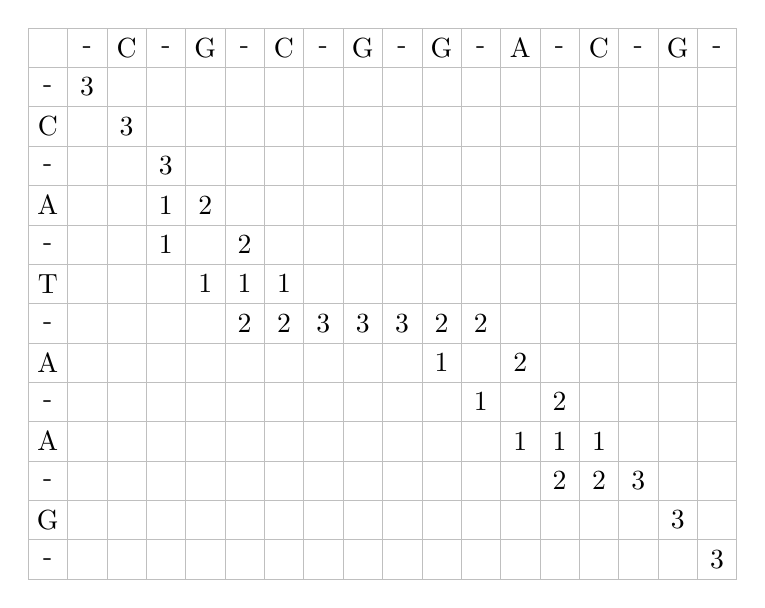
\begin{tikzpicture}[count/.style={color=black}]
\draw[very thin, color = gray!50, step = 0.5] (0,0) grid (9, 7);
\node at (0.25,6.25) {-};
\node at (0.25,5.75) {C};
\node at (0.25,5.25) {-};
\node at (0.25,4.75) {A};
\node at (0.25,4.25) {-};
\node at (0.25,3.75) {T};
\node at (0.25,3.25) {-};
\node at (0.25,2.75) {A};
\node at (0.25,2.25) {-};
\node at (0.25,1.75) {A};
\node at (0.25,1.25) {-};
\node at (0.25,0.75) {G};
\node at (0.25,0.25) {-};
\node at (0.75,6.75) {-};
\node at (1.25,6.75) {C};
\node at (1.75,6.75) {-};
\node at (2.25,6.75) {G};
\node at (2.75,6.75) {-};
\node at (3.25,6.75) {C};
\node at (3.75,6.75) {-};
\node at (4.25,6.75) {G};
\node at (4.75,6.75) {-};
\node at (5.25,6.75) {G};
\node at (5.75,6.75) {-};
\node at (6.25,6.75) {A};
\node at (6.75,6.75) {-};
\node at (7.25,6.75) {C};
\node at (7.75,6.75) {-};
\node at (8.25,6.75) {G};
\node at (8.75,6.75) {-};
\node[count] at (0.75, 6.25){3};
\node[count] at (1.25, 5.75){3};
\node[count] at (1.75, 5.25){3};
\node[count] at (1.75, 4.75){1};
\node[count] at (2.25, 4.75){2};
\node[count] at (1.75, 4.25){1};
\node[count] at (2.75, 4.25){2};
\node[count] at (2.25, 3.75){1};
\node[count] at (2.75, 3.75){1};
\node[count] at (3.25, 3.75){1};
\node[count] at (2.75, 3.25){2};
\node[count] at (3.25, 3.25){2};
\node[count] at (3.75, 3.25){3};
\node[count] at (4.25, 3.25){3};
\node[count] at (4.75, 3.25){3};
\node[count] at (5.25, 3.25){2};
\node[count] at (5.75, 3.25){2};
\node[count] at (5.25, 2.75){1};
\node[count] at (6.25, 2.75){2};
\node[count] at (5.75, 2.25){1};
\node[count] at (6.75, 2.25){2};
\node[count] at (6.25, 1.75){1};
\node[count] at (6.75, 1.75){1};
\node[count] at (7.25, 1.75){1};
\node[count] at (6.75, 1.25){2};
\node[count] at (7.25, 1.25){2};
\node[count] at (7.75, 1.25){3};
\node[count] at (8.25, 0.75){3};
\node[count] at (8.75, 0.25){3};
\end{tikzpicture}
}
        \caption{}
     \end{subfigure}
    % \begin{subfigure}[b]{0.49\textwidth}
    %     \centering
    %     \resizebox{1.3\textwidth}{!}{% Created by tikzDevice version 0.12.4 on 2023-10-07 18:20:52
% !TEX encoding = UTF-8 Unicode
\definecolor{color1}{HTML}{CC9966}
\definecolor{color2}{HTML}{99CCFF}
\definecolor{viridis0}{RGB}{255, 255, 255}
\definecolor{viridis1}{RGB}{253, 231, 37}
\definecolor{viridis2}{RGB}{181, 222, 43}
\definecolor{viridis3}{RGB}{110, 206, 88}
\definecolor{viridis4}{RGB}{53, 183, 121}
\definecolor{viridis5}{RGB}{31, 158, 137}
\definecolor{viridis6}{RGB}{38, 130, 142}
\definecolor{viridis7}{RGB}{49, 104, 142}
\definecolor{viridis8}{RGB}{62, 73, 137}
\definecolor{viridis9}{RGB}{72, 40, 120}
\definecolor{viridis10}{RGB}{68, 1, 84}
\begin{tikzpicture}[box/.style={rectangle, minimum size=0.5cm}]
\draw[very thin, color = gray!50, step = 0.5] (0,0) grid (9, 7);
\node at (0.25,6.25) {-};
\node at (0.25,5.75) {C};
\node at (0.25,5.25) {-};
\node at (0.25,4.75) {A};
\node at (0.25,4.25) {-};
\node at (0.25,3.75) {T};
\node at (0.25,3.25) {-};
\node at (0.25,2.75) {A};
\node at (0.25,2.25) {-};
\node at (0.25,1.75) {A};
\node at (0.25,1.25) {-};
\node at (0.25,0.75) {G};
\node at (0.25,0.25) {-};
\node at (0.75,6.75) {-};
\node at (1.25,6.75) {C};
\node at (1.75,6.75) {-};
\node at (2.25,6.75) {G};
\node at (2.75,6.75) {-};
\node at (3.25,6.75) {C};
\node at (3.75,6.75) {-};
\node at (4.25,6.75) {G};
\node at (4.75,6.75) {-};
\node at (5.25,6.75) {G};
\node at (5.75,6.75) {-};
\node at (6.25,6.75) {A};
\node at (6.75,6.75) {-};
\node at (7.25,6.75) {C};
\node at (7.75,6.75) {-};
\node at (8.25,6.75) {G};
\node at (8.75,6.75) {-};
\node[box, fill=viridis10] at (0.75, 6.25){};
\node[box, fill=viridis10] at (1.25, 5.75){};
\node[box, fill=viridis10] at (1.75, 5.25){};
\node[box, fill=viridis4] at (1.75, 4.75){};
\node[box, fill=viridis7] at (2.25, 4.75){};
\node[box, fill=viridis4] at (1.75, 4.25){};
\node[box, fill=viridis7] at (2.75, 4.25){};
\node[box, fill=viridis4] at (2.25, 3.75){};
\node[box, fill=viridis4] at (2.75, 3.75){};
\node[box, fill=viridis4] at (3.25, 3.75){};
\node[box, fill=viridis7] at (2.75, 3.25){};
\node[box, fill=viridis7] at (3.25, 3.25){};
\node[box, fill=viridis10] at (3.75, 3.25){};
\node[box, fill=viridis10] at (4.25, 3.25){};
\node[box, fill=viridis10] at (4.75, 3.25){};
\node[box, fill=viridis7] at (5.25, 3.25){};
\node[box, fill=viridis7] at (5.75, 3.25){};
\node[box, fill=viridis4] at (5.25, 2.75){};
\node[box, fill=viridis7] at (6.25, 2.75){};
\node[box, fill=viridis4] at (5.75, 2.25){};
\node[box, fill=viridis7] at (6.75, 2.25){};
\node[box, fill=viridis4] at (6.25, 1.75){};
\node[box, fill=viridis4] at (6.75, 1.75){};
\node[box, fill=viridis4] at (7.25, 1.75){};
\node[box, fill=viridis7] at (6.75, 1.25){};
\node[box, fill=viridis7] at (7.25, 1.25){};
\node[box, fill=viridis10] at (7.75, 1.25){};
\node[box, fill=viridis10] at (8.25, 0.75){};
\node[box, fill=viridis10] at (8.75, 0.25){};
\matrix [draw, below right, draw=none] at (current bounding box.north east) {
        % \node[box, fill=viridis0, scale=0.75] {0\%}; \\
        \node[box, fill=viridis1, scale=0.75] {00-09\%}; \\
        \node[box, fill=viridis2, scale=0.75] {10-19\%}; \\
        \node[box, fill=viridis3, scale=0.75] {20-29\%}; \\
        \node[box, fill=viridis4, scale=0.75] {30-29\%}; \\
        \node[box, fill=viridis5, scale=0.75] {\textcolor{white}{40-49\%}}; \\
        \node[box, fill=viridis6, scale=0.75] {\textcolor{white}{50-59\%}}; \\
        \node[box, fill=viridis7, scale=0.75] {\textcolor{white}{60-69\%}}; \\
        \node[box, fill=viridis8, scale=0.75] {\textcolor{white}{70-79\%}}; \\
        \node[box, fill=viridis9, scale=0.75] {\textcolor{white}{80-89\%}}; \\
        \node[box, fill=viridis10, scale=0.75] {\textcolor{white}{90-100\%}}; \\
    };
\end{tikzpicture}
}
    %     \caption{}
    %  \end{subfigure}
    \caption[Alignment to Expanded Dot Matrix]{Converting three alternative alignments to an expanded dot matrix. (a) is three alternative alignments of sequences $s$ and $v$. (b) is a matrix with the characters in sequence $s$ as rows and the characters in sequence $v$ as columns. In addition, gap symbols have been added to represent indel information. The values indicate the count of substitutions or indels between the row and column characters (i.e., the first `C' in both sequences is matched in all three alignments). Note empty cells have a count of zero, omitted here.}
    \label{fig:aln2matrix-expanded}
    % (c) is the dot matrix resulting from the alignment in (a), indicating where the substitutions and indel occur. Here colors are used to indicate the percentage of occurrences per event. Dark purple indicates the event is present in all three alignments (100\%), blue indicates 50\% (present in two alignments), and green indicates 33\% (only one alignment).}
\end{figure}

\subsection{Dot Plot Models}

\subsubsection{Traditional Model}

The traditional dot plot model resembles the original dot plots most, adapting the idea of identifying similarity between sequences to pairwise alignments. Consequently, this model only considers substitutions by using the traditional dot matrix. After calculating the counts for each cell, these are converted into frequencies. These values represent the percentage of alignments where each pair of symbols is aligned together. The final step is to draw squares on the tikz grid filled with a color corresponding to their frequency.

Figure \ref{fig:traditional} illustrates a traditional dot plot with three different alignments.
Diagonal rows of squares, running left to right and top to bottom, indicate regions of contiguous substitutions. In addition, darker sections are most common among the alignments, while lighter squares indicate less frequent pairings. This model retains the simplicity of dot plots and is an efficient tool for highlighting common substitution patterns in pairwise alignments. Furthermore, the traditional model is scalable to a large number of sequences.
\DIFdelbegin %DIFDELCMD < 

%DIFDELCMD < \begin{figure}[!ht]
%DIFDELCMD <     %%%
\DIFdelendFL \DIFaddbeginFL \begin{figure}[H]
    \DIFaddendFL \centering
    \begin{subfigure}[c]{0.2\textwidth}
        \centering
        \hspace*{-2em}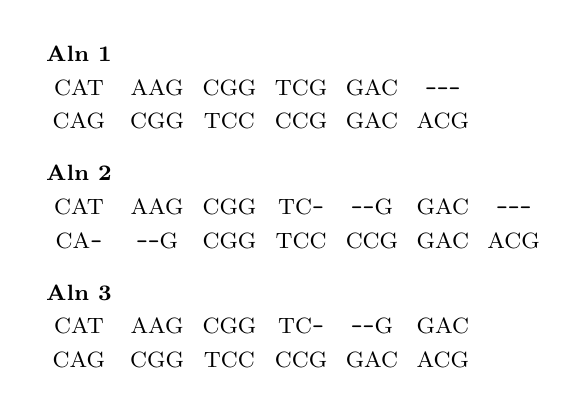
\begin{tikzpicture}[node distance=5mm,font=\footnotesize]
\tikzstyle{aln}=[matrix of nodes, nodes in empty cells]

\matrix (aln1)[aln] {
 \textbf{Aln 1} & & & & & &\\
CAT & AAG & CGG & TCG & GAC & \verb|---| &\\
CAG & CGG & TCC & CCG & GAC & ACG &\\
\\
 \textbf{Aln 2} & & & & & &\\
CAT & AAG & CGG & TC\verb|-| & \verb|--|G & GAC & \verb|---|\\
CA\verb|-| & \verb|--|G & CGG & TCC & CCG & GAC & ACG\\
\\
 \textbf{Aln 3} & & & & & &\\
CAT & AAG & CGG & TC\verb|-| & \verb|--|G & GAC &\\
CAG & CGG & TCC & CCG & GAC & ACG &\\
};
\end{tikzpicture}
        \vspace*{-1.5em}\caption{}
     \end{subfigure}
     \hspace{6em}
    \begin{subfigure}[c]{0.5\textwidth}
        \centering
        \resizebox{1.15\textwidth}{!}{% Created by tikzDevice version 0.12.5 on 2023-10-08 01:39:54
% !TEX encoding = UTF-8 Unicode
\definecolor{color1}{HTML}{CC9966}
\definecolor{color2}{HTML}{99CCFF}
\definecolor{viridis0}{RGB}{255, 255, 255}
\definecolor{viridis1}{RGB}{253, 231, 37}
\definecolor{viridis2}{RGB}{181, 222, 43}
\definecolor{viridis3}{RGB}{110, 206, 88}
\definecolor{viridis4}{RGB}{53, 183, 121}
\definecolor{viridis5}{RGB}{31, 158, 137}
\definecolor{viridis6}{RGB}{38, 130, 142}
\definecolor{viridis7}{RGB}{49, 104, 142}
\definecolor{viridis8}{RGB}{62, 73, 137}
\definecolor{viridis9}{RGB}{72, 40, 120}
\definecolor{viridis10}{RGB}{68, 1, 84}
\begin{tikzpicture}[box/.style={rectangle, fill=gray!50, minimum size=0.5cm}]
\draw[very thin, color = gray!50, step = 0.5] (0,0) grid (9.5, 8);
\node at (0.25,7.25) {C};
\node at (0.25,6.75) {A};
\node at (0.25,6.25) {T};
\node at (0.25,5.75) {A};
\node at (0.25,5.25) {A};
\node at (0.25,4.75) {G};
\node at (0.25,4.25) {C};
\node at (0.25,3.75) {G};
\node at (0.25,3.25) {G};
\node at (0.25,2.75) {T};
\node at (0.25,2.25) {C};
\node at (0.25,1.75) {G};
\node at (0.25,1.25) {G};
\node at (0.25,0.75) {A};
\node at (0.25,0.25) {C};
\node at (0.75,7.75) {C};
\node at (1.25,7.75) {A};
\node at (1.75,7.75) {G};
\node at (2.25,7.75) {C};
\node at (2.75,7.75) {G};
\node at (3.25,7.75) {G};
\node at (3.75,7.75) {T};
\node at (4.25,7.75) {C};
\node at (4.75,7.75) {C};
\node at (5.25,7.75) {C};
\node at (5.75,7.75) {C};
\node at (6.25,7.75) {G};
\node at (6.75,7.75) {G};
\node at (7.25,7.75) {A};
\node at (7.75,7.75) {C};
\node at (8.25,7.75) {A};
\node at (8.75,7.75) {C};
\node at (9.25,7.75) {G};
\node[box, fill=viridis10] at (0.75, 7.25){};
\node[box, fill=viridis10] at (1.25, 6.75){};
\node[box, fill=viridis7] at (1.75, 6.25){};
\node[box, fill=viridis7] at (2.25, 5.75){};
\node[box, fill=viridis7] at (2.75, 5.25){};
\node[box, fill=viridis4] at (1.75, 4.75){};
\node[box, fill=viridis7] at (3.25, 4.75){};
\node[box, fill=viridis4] at (2.25, 4.25){};
\node[box, fill=viridis7] at (3.75, 4.25){};
\node[box, fill=viridis4] at (2.75, 3.75){};
\node[box, fill=viridis7] at (4.25, 3.75){};
\node[box, fill=viridis4] at (3.25, 3.25){};
\node[box, fill=viridis7] at (4.75, 3.25){};
\node[box, fill=viridis4] at (3.75, 2.75){};
\node[box, fill=viridis7] at (5.25, 2.75){};
\node[box, fill=viridis4] at (4.25, 2.25){};
\node[box, fill=viridis7] at (5.75, 2.25){};
\node[box, fill=viridis7] at (6.25, 1.75){};
\node[box, fill=viridis4] at (7.75, 1.75){};
\node[box, fill=viridis7] at (6.75, 1.25){};
\node[box, fill=viridis4] at (8.25, 1.25){};
\node[box, fill=viridis7] at (7.25, 0.75){};
\node[box, fill=viridis4] at (8.75, 0.75){};
\node[box, fill=viridis7] at (7.75, 0.25){};
\node[box, fill=viridis4] at (9.25, 0.25){};
\matrix [draw, below right, draw=none] at (current bounding box.north east) {
        % \node[box, fill=viridis0, scale=0.75] {0\%}; \\
        \node[box, fill=viridis1, scale=0.75] {00-09\%}; \\
        \node[box, fill=viridis2, scale=0.75] {10-19\%}; \\
        \node[box, fill=viridis3, scale=0.75] {20-29\%}; \\
        \node[box, fill=viridis4, scale=0.75] {30-29\%}; \\
        \node[box, fill=viridis5, scale=0.75] {\textcolor{white}{40-49\%}}; \\
        \node[box, fill=viridis6, scale=0.75] {\textcolor{white}{50-59\%}}; \\
        \node[box, fill=viridis7, scale=0.75] {\textcolor{white}{60-69\%}}; \\
        \node[box, fill=viridis8, scale=0.75] {\textcolor{white}{70-79\%}}; \\
        \node[box, fill=viridis9, scale=0.75] {\textcolor{white}{80-89\%}}; \\
        \node[box, fill=viridis10, scale=0.75] {\textcolor{white}{90-100\%}}; \\
    };
\end{tikzpicture}
}
        \caption{}
     \end{subfigure}
    \caption[Traditional Dot Plot Model]{Example of a traditional alignment dot plot of three possible pairwise alignments. Squares represent matching and mismatching nucleotides, while the color gradient indicates their frequency in the alignments. The first two nucleotides `C' and `A' are matched in all three alignments (100\%). The remaining squares on the main diagonal are only shared in two alignments (66\%), while the remaining squares are only present in one alignment (33\%).}
    \label{fig:traditional}
\end{figure}

\subsubsection{Expanded Model}
% adds information about indels

% using extended dot matrix - check name
% more similar to NW, SW, and Gotoh alignment matrices
% In addition to diagonals, now moving right or below indicates indels
% double in size
% more informative, yet "high traffic sections" are indistinguishable
The expanded model includes information about indel events and therefore uses an expanded dot matrix to store alignment counts. These plots are conceptually similar to conventional visual aids to explain Needleman-Wunsch \citep{Needleman1970} or Gotoh \citep{gotoh_1982} algorithms where an alignment is illustrated as the path through a matrix. In comparison to the previous model, these plots add gap symbols between the characters of each sequence and are used to mark indel events. However, the process of creating the tikz grid with squares is similar. Counts are converted to frequencies and used to fill the squares in the matrix with the appropriate color. This model can easily accommodate large amounts of alignments.

\begin{figure}[!ht]
    \centering
    \begin{subfigure}[c]{0.2\textwidth}
        \centering
        \hspace*{-2em}\scalebox{0.8}{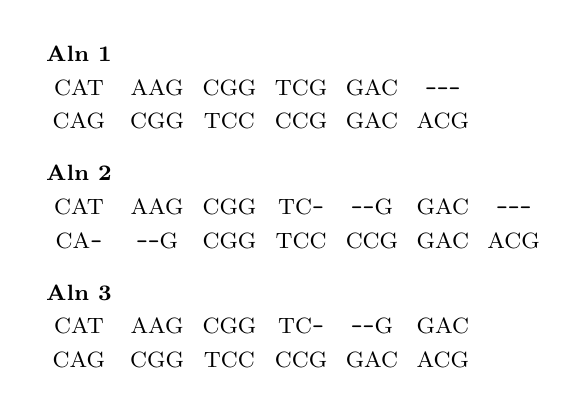
\begin{tikzpicture}[node distance=5mm,font=\footnotesize]
\tikzstyle{aln}=[matrix of nodes, nodes in empty cells]

\matrix (aln1)[aln] {
 \textbf{Aln 1} & & & & & &\\
CAT & AAG & CGG & TCG & GAC & \verb|---| &\\
CAG & CGG & TCC & CCG & GAC & ACG &\\
\\
 \textbf{Aln 2} & & & & & &\\
CAT & AAG & CGG & TC\verb|-| & \verb|--|G & GAC & \verb|---|\\
CA\verb|-| & \verb|--|G & CGG & TCC & CCG & GAC & ACG\\
\\
 \textbf{Aln 3} & & & & & &\\
CAT & AAG & CGG & TC\verb|-| & \verb|--|G & GAC &\\
CAG & CGG & TCC & CCG & GAC & ACG &\\
};
\end{tikzpicture}}
        \vspace*{-1.5em}\caption{}
     \end{subfigure}
     \hspace{3.2em}
    \begin{subfigure}[c]{0.5\textwidth}
        \centering
        \resizebox{1.3\textwidth}{!}{% Created by tikzDevice version 0.12.5 on 2023-10-08 01:40:20
% !TEX encoding = UTF-8 Unicode
\definecolor{color1}{HTML}{CC9966}
\definecolor{color2}{HTML}{99CCFF}
\definecolor{viridis0}{RGB}{255, 255, 255}
\definecolor{viridis1}{RGB}{253, 231, 37}
\definecolor{viridis2}{RGB}{181, 222, 43}
\definecolor{viridis3}{RGB}{110, 206, 88}
\definecolor{viridis4}{RGB}{53, 183, 121}
\definecolor{viridis5}{RGB}{31, 158, 137}
\definecolor{viridis6}{RGB}{38, 130, 142}
\definecolor{viridis7}{RGB}{49, 104, 142}
\definecolor{viridis8}{RGB}{62, 73, 137}
\definecolor{viridis9}{RGB}{72, 40, 120}
\definecolor{viridis10}{RGB}{68, 1, 84}
\begin{tikzpicture}[box/.style={rectangle, minimum size=0.5cm}]
\draw[very thin, color = gray!50, step = 0.5] (0,0) grid (19, 16);
\node at (0.25,15.25) {-};
\node at (0.25,14.75) {C};
\node at (0.25,14.25) {-};
\node at (0.25,13.75) {A};
\node at (0.25,13.25) {-};
\node at (0.25,12.75) {T};
\node at (0.25,12.25) {-};
\node at (0.25,11.75) {A};
\node at (0.25,11.25) {-};
\node at (0.25,10.75) {A};
\node at (0.25,10.25) {-};
\node at (0.25,9.75) {G};
\node at (0.25,9.25) {-};
\node at (0.25,8.75) {C};
\node at (0.25,8.25) {-};
\node at (0.25,7.75) {G};
\node at (0.25,7.25) {-};
\node at (0.25,6.75) {G};
\node at (0.25,6.25) {-};
\node at (0.25,5.75) {T};
\node at (0.25,5.25) {-};
\node at (0.25,4.75) {C};
\node at (0.25,4.25) {-};
\node at (0.25,3.75) {G};
\node at (0.25,3.25) {-};
\node at (0.25,2.75) {G};
\node at (0.25,2.25) {-};
\node at (0.25,1.75) {A};
\node at (0.25,1.25) {-};
\node at (0.25,0.75) {C};
\node at (0.25,0.25) {-};
\node at (0.75,15.75) {-};
\node at (1.25,15.75) {C};
\node at (1.75,15.75) {-};
\node at (2.25,15.75) {A};
\node at (2.75,15.75) {-};
\node at (3.25,15.75) {G};
\node at (3.75,15.75) {-};
\node at (4.25,15.75) {C};
\node at (4.75,15.75) {-};
\node at (5.25,15.75) {G};
\node at (5.75,15.75) {-};
\node at (6.25,15.75) {G};
\node at (6.75,15.75) {-};
\node at (7.25,15.75) {T};
\node at (7.75,15.75) {-};
\node at (8.25,15.75) {C};
\node at (8.75,15.75) {-};
\node at (9.25,15.75) {C};
\node at (9.75,15.75) {-};
\node at (10.25,15.75) {C};
\node at (10.75,15.75) {-};
\node at (11.25,15.75) {C};
\node at (11.75,15.75) {-};
\node at (12.25,15.75) {G};
\node at (12.75,15.75) {-};
\node at (13.25,15.75) {G};
\node at (13.75,15.75) {-};
\node at (14.25,15.75) {A};
\node at (14.75,15.75) {-};
\node at (15.25,15.75) {C};
\node at (15.75,15.75) {-};
\node at (16.25,15.75) {A};
\node at (16.75,15.75) {-};
\node at (17.25,15.75) {C};
\node at (17.75,15.75) {-};
\node at (18.25,15.75) {G};
\node at (18.75,15.75) {-};
\node[box, fill=viridis10] at (0.75, 15.25){};
\node[box, fill=viridis10] at (1.25, 14.75){};
\node[box, fill=viridis10] at (1.75, 14.25){};
\node[box, fill=viridis10] at (2.25, 13.75){};
\node[box, fill=viridis10] at (2.75, 13.25){};
\node[box, fill=viridis4] at (2.75, 12.75){};
\node[box, fill=viridis7] at (3.25, 12.75){};
\node[box, fill=viridis4] at (2.75, 12.25){};
\node[box, fill=viridis7] at (3.75, 12.25){};
\node[box, fill=viridis4] at (2.75, 11.75){};
\node[box, fill=viridis7] at (4.25, 11.75){};
\node[box, fill=viridis4] at (2.75, 11.25){};
\node[box, fill=viridis7] at (4.75, 11.25){};
\node[box, fill=viridis4] at (2.75, 10.75){};
\node[box, fill=viridis7] at (5.25, 10.75){};
\node[box, fill=viridis4] at (2.75, 10.25){};
\node[box, fill=viridis7] at (5.75, 10.25){};
\node[box, fill=viridis4] at (3.25, 9.75){};
\node[box, fill=viridis7] at (6.25, 9.75){};
\node[box, fill=viridis4] at (3.75, 9.25){};
\node[box, fill=viridis7] at (6.75, 9.25){};
\node[box, fill=viridis4] at (4.25, 8.75){};
\node[box, fill=viridis7] at (7.25, 8.75){};
\node[box, fill=viridis4] at (4.75, 8.25){};
\node[box, fill=viridis7] at (7.75, 8.25){};
\node[box, fill=viridis4] at (5.25, 7.75){};
\node[box, fill=viridis7] at (8.25, 7.75){};
\node[box, fill=viridis4] at (5.75, 7.25){};
\node[box, fill=viridis7] at (8.75, 7.25){};
\node[box, fill=viridis4] at (6.25, 6.75){};
\node[box, fill=viridis7] at (9.25, 6.75){};
\node[box, fill=viridis4] at (6.75, 6.25){};
\node[box, fill=viridis7] at (9.75, 6.25){};
\node[box, fill=viridis4] at (7.25, 5.75){};
\node[box, fill=viridis7] at (10.25, 5.75){};
\node[box, fill=viridis4] at (7.75, 5.25){};
\node[box, fill=viridis7] at (10.75, 5.25){};
\node[box, fill=viridis4] at (8.25, 4.75){};
\node[box, fill=viridis7] at (11.25, 4.75){};
\node[box, fill=viridis4] at (8.75, 4.25){};
\node[box, fill=viridis4] at (9.25, 4.25){};
\node[box, fill=viridis4] at (9.75, 4.25){};
\node[box, fill=viridis4] at (10.25, 4.25){};
\node[box, fill=viridis4] at (10.75, 4.25){};
\node[box, fill=viridis4] at (11.25, 4.25){};
\node[box, fill=viridis10] at (11.75, 4.25){};
\node[box, fill=viridis4] at (12.25, 4.25){};
\node[box, fill=viridis4] at (12.75, 4.25){};
\node[box, fill=viridis4] at (13.25, 4.25){};
\node[box, fill=viridis4] at (13.75, 4.25){};
\node[box, fill=viridis4] at (14.25, 4.25){};
\node[box, fill=viridis4] at (14.75, 4.25){};
\node[box, fill=viridis7] at (12.25, 3.75){};
\node[box, fill=viridis4] at (15.25, 3.75){};
\node[box, fill=viridis7] at (12.75, 3.25){};
\node[box, fill=viridis4] at (15.75, 3.25){};
\node[box, fill=viridis7] at (13.25, 2.75){};
\node[box, fill=viridis4] at (16.25, 2.75){};
\node[box, fill=viridis7] at (13.75, 2.25){};
\node[box, fill=viridis4] at (16.75, 2.25){};
\node[box, fill=viridis7] at (14.25, 1.75){};
\node[box, fill=viridis4] at (17.25, 1.75){};
\node[box, fill=viridis7] at (14.75, 1.25){};
\node[box, fill=viridis4] at (17.75, 1.25){};
\node[box, fill=viridis7] at (15.25, 0.75){};
\node[box, fill=viridis4] at (18.25, 0.75){};
\node[box, fill=viridis7] at (15.75, 0.25){};
\node[box, fill=viridis7] at (16.25, 0.25){};
\node[box, fill=viridis7] at (16.75, 0.25){};
\node[box, fill=viridis7] at (17.25, 0.25){};
\node[box, fill=viridis7] at (17.75, 0.25){};
\node[box, fill=viridis7] at (18.25, 0.25){};
\node[box, fill=viridis10] at (18.75, 0.25){};
\matrix [draw, below right, draw=none] at (current bounding box.north east) {
        % \node[box, fill=viridis0, scale=0.75] {0\%}; \\
        \node[box, fill=viridis1, scale=0.75] {00-09\%}; \\
        \node[box, fill=viridis2, scale=0.75] {10-19\%}; \\
        \node[box, fill=viridis3, scale=0.75] {20-29\%}; \\
        \node[box, fill=viridis4, scale=0.75] {30-29\%}; \\
        \node[box, fill=viridis5, scale=0.75] {\textcolor{white}{40-49\%}}; \\
        \node[box, fill=viridis6, scale=0.75] {\textcolor{white}{50-59\%}}; \\
        \node[box, fill=viridis7, scale=0.75] {\textcolor{white}{60-69\%}}; \\
        \node[box, fill=viridis8, scale=0.75] {\textcolor{white}{70-79\%}}; \\
        \node[box, fill=viridis9, scale=0.75] {\textcolor{white}{80-89\%}}; \\
        \node[box, fill=viridis10, scale=0.75] {\textcolor{white}{90-100\%}}; \\
    };
\end{tikzpicture}
}
        \caption{}
     \end{subfigure}
    \caption[Expanded Dot Plot Model]{Example of an expanded alignment dot plot for three possible pairwise alignments. Squares indicate substitution, insertion, or deletion events between symbols of the sequences. Diagonal rows of squares represent substitutions, while vertical and horizontal contiguous squares represent deletions and insertions, respectively. Colors indicate the frequency of events in the alignments.}
    \label{fig:expanded}
\end{figure}

Figure \ref{fig:expanded} illustrates how an expanded dot plot is created from the same three pairwise alignments as in the previous model. In addition to the diagonals of squares that indicate substitutions, this plot provides information about how they are connected. Furthermore, the expanded model uncovers a high-traffic section where paths cross, a cell connecting two gap symbols with 100\% frequency.

\subsubsection{Line Model}

% adds path identification, clarifying congested areas
The line model introduces a new concept of nodes connected with edges to form a path or line.
\DIFdelbegin \DIFdel{Nodes replace the squares from previous models }\DIFdelend \DIFaddbegin \DIFadd{The nodes represent events in the alignment, while the edges connect pairs of cells in an alignment matrix. This model is an evolution of the expanded model, where the events are alignment events are marked }\DIFaddend and the edges clarify the transition between them. The line in a plot can split into different branches, indicating sections where the alignments are different. An expanded dot matrix is used to build a line dot plot. Similarly to the previous models, counts are converted to frequencies and used to fill the nodes with the corresponding color. However, the line model utilizes three matrices to store substitutions, insertions, and deletions separately, needed to identify source and destination information to plot the edges. In addition, the edges are colored with the frequency of the destination node. This model can be seen as an extension of the expanded model that unveils information about high-traffic nodes and introduces the concept of a path, which will be useful later. Furthermore, this model is easily scalable to large amounts of data.

Figure \ref{fig:line} illustrates the line alignment dot plot resulting from three alignments. In comparison to the expanded model, figure \ref{fig:line}-b helps disentangle the alignment path in congested areas such as the node where the three alignments, represented by two different branches, cross.

\clearpage

\begin{figure}[!htb]
    \centering
    \begin{subfigure}[c]{0.2\textwidth}
        \centering
        \vspace*{4em}\hspace*{-4em}\scalebox{0.8}{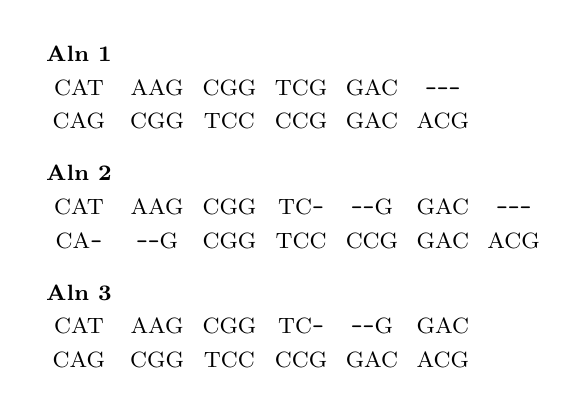
\begin{tikzpicture}[node distance=5mm,font=\footnotesize]
\tikzstyle{aln}=[matrix of nodes, nodes in empty cells]

\matrix (aln1)[aln] {
 \textbf{Aln 1} & & & & & &\\
CAT & AAG & CGG & TCG & GAC & \verb|---| &\\
CAG & CGG & TCC & CCG & GAC & ACG &\\
\\
 \textbf{Aln 2} & & & & & &\\
CAT & AAG & CGG & TC\verb|-| & \verb|--|G & GAC & \verb|---|\\
CA\verb|-| & \verb|--|G & CGG & TCC & CCG & GAC & ACG\\
\\
 \textbf{Aln 3} & & & & & &\\
CAT & AAG & CGG & TC\verb|-| & \verb|--|G & GAC &\\
CAG & CGG & TCC & CCG & GAC & ACG &\\
};
\end{tikzpicture}}
        \vspace*{1em}\caption{}
     \end{subfigure}
     \hspace{3.2em}
    \begin{subfigure}[c]{0.5\textwidth}
        \centering
        \DIFdelbeginFL %DIFDELCMD < \resizebox{1.3\textwidth}{!}{% Created by tikzDevice version 0.12.5 on 2023-10-08 01:42:03
%DIFDELCMD < % !TEX encoding = UTF-8 Unicode
%DIFDELCMD < \definecolor{color1}{HTML}{CC9966}
%DIFDELCMD < \definecolor{color2}{HTML}{99CCFF}
%DIFDELCMD < \definecolor{viridis0}{RGB}{255, 255, 255}
%DIFDELCMD < \definecolor{viridis1}{RGB}{253, 231, 37}
%DIFDELCMD < \definecolor{viridis2}{RGB}{181, 222, 43}
%DIFDELCMD < \definecolor{viridis3}{RGB}{110, 206, 88}
%DIFDELCMD < \definecolor{viridis4}{RGB}{53, 183, 121}
%DIFDELCMD < \definecolor{viridis5}{RGB}{31, 158, 137}
%DIFDELCMD < \definecolor{viridis6}{RGB}{38, 130, 142}
%DIFDELCMD < \definecolor{viridis7}{RGB}{49, 104, 142}
%DIFDELCMD < \definecolor{viridis8}{RGB}{62, 73, 137}
%DIFDELCMD < \definecolor{viridis9}{RGB}{72, 40, 120}
%DIFDELCMD < \definecolor{viridis10}{RGB}{68, 1, 84}
%DIFDELCMD < \begin{tikzpicture}[dot/.style={circle, minimum size=2.5mm}]
%DIFDELCMD < \draw[very thin, color = gray!50, step = 0.5] (0,0) grid (19, 16);
%DIFDELCMD < \node at (0.25,15.25) {-};
%DIFDELCMD < \node at (0.25,14.75) {C};
%DIFDELCMD < \node at (0.25,14.25) {-};
%DIFDELCMD < \node at (0.25,13.75) {A};
%DIFDELCMD < \node at (0.25,13.25) {-};
%DIFDELCMD < \node at (0.25,12.75) {T};
%DIFDELCMD < \node at (0.25,12.25) {-};
%DIFDELCMD < \node at (0.25,11.75) {A};
%DIFDELCMD < \node at (0.25,11.25) {-};
%DIFDELCMD < \node at (0.25,10.75) {A};
%DIFDELCMD < \node at (0.25,10.25) {-};
%DIFDELCMD < \node at (0.25,9.75) {G};
%DIFDELCMD < \node at (0.25,9.25) {-};
%DIFDELCMD < \node at (0.25,8.75) {C};
%DIFDELCMD < \node at (0.25,8.25) {-};
%DIFDELCMD < \node at (0.25,7.75) {G};
%DIFDELCMD < \node at (0.25,7.25) {-};
%DIFDELCMD < \node at (0.25,6.75) {G};
%DIFDELCMD < \node at (0.25,6.25) {-};
%DIFDELCMD < \node at (0.25,5.75) {T};
%DIFDELCMD < \node at (0.25,5.25) {-};
%DIFDELCMD < \node at (0.25,4.75) {C};
%DIFDELCMD < \node at (0.25,4.25) {-};
%DIFDELCMD < \node at (0.25,3.75) {G};
%DIFDELCMD < \node at (0.25,3.25) {-};
%DIFDELCMD < \node at (0.25,2.75) {G};
%DIFDELCMD < \node at (0.25,2.25) {-};
%DIFDELCMD < \node at (0.25,1.75) {A};
%DIFDELCMD < \node at (0.25,1.25) {-};
%DIFDELCMD < \node at (0.25,0.75) {C};
%DIFDELCMD < \node at (0.25,0.25) {-};
%DIFDELCMD < \node at (0.75,15.75) {-};
%DIFDELCMD < \node at (1.25,15.75) {C};
%DIFDELCMD < \node at (1.75,15.75) {-};
%DIFDELCMD < \node at (2.25,15.75) {A};
%DIFDELCMD < \node at (2.75,15.75) {-};
%DIFDELCMD < \node at (3.25,15.75) {G};
%DIFDELCMD < \node at (3.75,15.75) {-};
%DIFDELCMD < \node at (4.25,15.75) {C};
%DIFDELCMD < \node at (4.75,15.75) {-};
%DIFDELCMD < \node at (5.25,15.75) {G};
%DIFDELCMD < \node at (5.75,15.75) {-};
%DIFDELCMD < \node at (6.25,15.75) {G};
%DIFDELCMD < \node at (6.75,15.75) {-};
%DIFDELCMD < \node at (7.25,15.75) {T};
%DIFDELCMD < \node at (7.75,15.75) {-};
%DIFDELCMD < \node at (8.25,15.75) {C};
%DIFDELCMD < \node at (8.75,15.75) {-};
%DIFDELCMD < \node at (9.25,15.75) {C};
%DIFDELCMD < \node at (9.75,15.75) {-};
%DIFDELCMD < \node at (10.25,15.75) {C};
%DIFDELCMD < \node at (10.75,15.75) {-};
%DIFDELCMD < \node at (11.25,15.75) {C};
%DIFDELCMD < \node at (11.75,15.75) {-};
%DIFDELCMD < \node at (12.25,15.75) {G};
%DIFDELCMD < \node at (12.75,15.75) {-};
%DIFDELCMD < \node at (13.25,15.75) {G};
%DIFDELCMD < \node at (13.75,15.75) {-};
%DIFDELCMD < \node at (14.25,15.75) {A};
%DIFDELCMD < \node at (14.75,15.75) {-};
%DIFDELCMD < \node at (15.25,15.75) {C};
%DIFDELCMD < \node at (15.75,15.75) {-};
%DIFDELCMD < \node at (16.25,15.75) {A};
%DIFDELCMD < \node at (16.75,15.75) {-};
%DIFDELCMD < \node at (17.25,15.75) {C};
%DIFDELCMD < \node at (17.75,15.75) {-};
%DIFDELCMD < \node at (18.25,15.75) {G};
%DIFDELCMD < \node at (18.75,15.75) {-};
%DIFDELCMD < \draw[line width=1.25mm,viridis10](0.75,15.25)--(1.25,14.75);
%DIFDELCMD < \node[circle, fill=viridis10] at (0.75, 15.25){};
%DIFDELCMD < \draw[line width=1.25mm,viridis10](1.25,14.75)--(1.75,14.25);
%DIFDELCMD < \node[circle, fill=viridis10] at (1.25, 14.75){};
%DIFDELCMD < \draw[line width=1.25mm,viridis10](1.75,14.25)--(2.25,13.75);
%DIFDELCMD < \node[circle, fill=viridis10] at (1.75, 14.25){};
%DIFDELCMD < \draw[line width=1.25mm,viridis10](2.25,13.75)--(2.75,13.25);
%DIFDELCMD < \node[circle, fill=viridis10] at (2.25, 13.75){};
%DIFDELCMD < \draw[line width=1.25mm,viridis4](2.75,13.25)--(2.75,12.75);
%DIFDELCMD < \draw[line width=1.25mm,viridis7](2.75,13.25)--(3.25,12.75);
%DIFDELCMD < \node[circle, fill=viridis10] at (2.75, 13.25){};
%DIFDELCMD < \draw[line width=1.25mm,viridis4](2.75,12.75)--(2.75,12.25);
%DIFDELCMD < \node[circle, fill=viridis4] at (2.75, 12.75){};
%DIFDELCMD < \draw[line width=1.25mm,viridis7](3.25,12.75)--(3.75,12.25);
%DIFDELCMD < \node[circle, fill=viridis7] at (3.25, 12.75){};
%DIFDELCMD < \draw[line width=1.25mm,viridis4](2.75,12.25)--(2.75,11.75);
%DIFDELCMD < \node[circle, fill=viridis4] at (2.75, 12.25){};
%DIFDELCMD < \draw[line width=1.25mm,viridis7](3.75,12.25)--(4.25,11.75);
%DIFDELCMD < \node[circle, fill=viridis7] at (3.75, 12.25){};
%DIFDELCMD < \draw[line width=1.25mm,viridis4](2.75,11.75)--(2.75,11.25);
%DIFDELCMD < \node[circle, fill=viridis4] at (2.75, 11.75){};
%DIFDELCMD < \draw[line width=1.25mm,viridis7](4.25,11.75)--(4.75,11.25);
%DIFDELCMD < \node[circle, fill=viridis7] at (4.25, 11.75){};
%DIFDELCMD < \draw[line width=1.25mm,viridis4](2.75,11.25)--(2.75,10.75);
%DIFDELCMD < \node[circle, fill=viridis4] at (2.75, 11.25){};
%DIFDELCMD < \draw[line width=1.25mm,viridis7](4.75,11.25)--(5.25,10.75);
%DIFDELCMD < \node[circle, fill=viridis7] at (4.75, 11.25){};
%DIFDELCMD < \draw[line width=1.25mm,viridis4](2.75,10.75)--(2.75,10.25);
%DIFDELCMD < \node[circle, fill=viridis4] at (2.75, 10.75){};
%DIFDELCMD < \draw[line width=1.25mm,viridis7](5.25,10.75)--(5.75,10.25);
%DIFDELCMD < \node[circle, fill=viridis7] at (5.25, 10.75){};
%DIFDELCMD < \draw[line width=1.25mm,viridis4](2.75,10.25)--(3.25,9.75);
%DIFDELCMD < \node[circle, fill=viridis4] at (2.75, 10.25){};
%DIFDELCMD < \draw[line width=1.25mm,viridis7](5.75,10.25)--(6.25,9.75);
%DIFDELCMD < \node[circle, fill=viridis7] at (5.75, 10.25){};
%DIFDELCMD < \draw[line width=1.25mm,viridis4](3.25,9.75)--(3.75,9.25);
%DIFDELCMD < \node[circle, fill=viridis4] at (3.25, 9.75){};
%DIFDELCMD < \draw[line width=1.25mm,viridis7](6.25,9.75)--(6.75,9.25);
%DIFDELCMD < \node[circle, fill=viridis7] at (6.25, 9.75){};
%DIFDELCMD < \draw[line width=1.25mm,viridis4](3.75,9.25)--(4.25,8.75);
%DIFDELCMD < \node[circle, fill=viridis4] at (3.75, 9.25){};
%DIFDELCMD < \draw[line width=1.25mm,viridis7](6.75,9.25)--(7.25,8.75);
%DIFDELCMD < \node[circle, fill=viridis7] at (6.75, 9.25){};
%DIFDELCMD < \draw[line width=1.25mm,viridis4](4.25,8.75)--(4.75,8.25);
%DIFDELCMD < \node[circle, fill=viridis4] at (4.25, 8.75){};
%DIFDELCMD < \draw[line width=1.25mm,viridis7](7.25,8.75)--(7.75,8.25);
%DIFDELCMD < \node[circle, fill=viridis7] at (7.25, 8.75){};
%DIFDELCMD < \draw[line width=1.25mm,viridis4](4.75,8.25)--(5.25,7.75);
%DIFDELCMD < \node[circle, fill=viridis4] at (4.75, 8.25){};
%DIFDELCMD < \draw[line width=1.25mm,viridis7](7.75,8.25)--(8.25,7.75);
%DIFDELCMD < \node[circle, fill=viridis7] at (7.75, 8.25){};
%DIFDELCMD < \draw[line width=1.25mm,viridis4](5.25,7.75)--(5.75,7.25);
%DIFDELCMD < \node[circle, fill=viridis4] at (5.25, 7.75){};
%DIFDELCMD < \draw[line width=1.25mm,viridis7](8.25,7.75)--(8.75,7.25);
%DIFDELCMD < \node[circle, fill=viridis7] at (8.25, 7.75){};
%DIFDELCMD < \draw[line width=1.25mm,viridis4](5.75,7.25)--(6.25,6.75);
%DIFDELCMD < \node[circle, fill=viridis4] at (5.75, 7.25){};
%DIFDELCMD < \draw[line width=1.25mm,viridis7](8.75,7.25)--(9.25,6.75);
%DIFDELCMD < \node[circle, fill=viridis7] at (8.75, 7.25){};
%DIFDELCMD < \draw[line width=1.25mm,viridis4](6.25,6.75)--(6.75,6.25);
%DIFDELCMD < \node[circle, fill=viridis4] at (6.25, 6.75){};
%DIFDELCMD < \draw[line width=1.25mm,viridis7](9.25,6.75)--(9.75,6.25);
%DIFDELCMD < \node[circle, fill=viridis7] at (9.25, 6.75){};
%DIFDELCMD < \draw[line width=1.25mm,viridis4](6.75,6.25)--(7.25,5.75);
%DIFDELCMD < \node[circle, fill=viridis4] at (6.75, 6.25){};
%DIFDELCMD < \draw[line width=1.25mm,viridis7](9.75,6.25)--(10.25,5.75);
%DIFDELCMD < \node[circle, fill=viridis7] at (9.75, 6.25){};
%DIFDELCMD < \draw[line width=1.25mm,viridis4](7.25,5.75)--(7.75,5.25);
%DIFDELCMD < \node[circle, fill=viridis4] at (7.25, 5.75){};
%DIFDELCMD < \draw[line width=1.25mm,viridis7](10.25,5.75)--(10.75,5.25);
%DIFDELCMD < \node[circle, fill=viridis7] at (10.25, 5.75){};
%DIFDELCMD < \draw[line width=1.25mm,viridis4](7.75,5.25)--(8.25,4.75);
%DIFDELCMD < \node[circle, fill=viridis4] at (7.75, 5.25){};
%DIFDELCMD < \draw[line width=1.25mm,viridis7](10.75,5.25)--(11.25,4.75);
%DIFDELCMD < \node[circle, fill=viridis7] at (10.75, 5.25){};
%DIFDELCMD < \draw[line width=1.25mm,viridis4](8.25,4.75)--(8.75,4.25);
%DIFDELCMD < \node[circle, fill=viridis4] at (8.25, 4.75){};
%DIFDELCMD < \draw[line width=1.25mm,viridis7](11.25,4.75)--(11.75,4.25);
%DIFDELCMD < \node[circle, fill=viridis7] at (11.25, 4.75){};
%DIFDELCMD < \draw[line width=1.25mm,viridis4](8.75,4.25)--(9.25,4.25);
%DIFDELCMD < \node[circle, fill=viridis4] at (8.75, 4.25){};
%DIFDELCMD < \draw[line width=1.25mm,viridis4](9.25,4.25)--(9.75,4.25);
%DIFDELCMD < \node[circle, fill=viridis4] at (9.25, 4.25){};
%DIFDELCMD < \draw[line width=1.25mm,viridis4](9.75,4.25)--(10.25,4.25);
%DIFDELCMD < \node[circle, fill=viridis4] at (9.75, 4.25){};
%DIFDELCMD < \draw[line width=1.25mm,viridis4](10.25,4.25)--(10.75,4.25);
%DIFDELCMD < \node[circle, fill=viridis4] at (10.25, 4.25){};
%DIFDELCMD < \draw[line width=1.25mm,viridis4](10.75,4.25)--(11.25,4.25);
%DIFDELCMD < \node[circle, fill=viridis4] at (10.75, 4.25){};
%DIFDELCMD < \draw[line width=1.25mm,viridis4](11.25,4.25)--(11.75,4.25);
%DIFDELCMD < \node[circle, fill=viridis4] at (11.25, 4.25){};
%DIFDELCMD < \draw[line width=1.25mm,viridis4](11.75,4.25)--(12.25,4.25);
%DIFDELCMD < \draw[line width=1.25mm,viridis7](11.75,4.25)--(12.25,3.75);
%DIFDELCMD < \node[circle, fill=viridis10] at (11.75, 4.25){};
%DIFDELCMD < \draw[line width=1.25mm,viridis4](12.25,4.25)--(12.75,4.25);
%DIFDELCMD < \node[circle, fill=viridis4] at (12.25, 4.25){};
%DIFDELCMD < \draw[line width=1.25mm,viridis4](12.75,4.25)--(13.25,4.25);
%DIFDELCMD < \node[circle, fill=viridis4] at (12.75, 4.25){};
%DIFDELCMD < \draw[line width=1.25mm,viridis4](13.25,4.25)--(13.75,4.25);
%DIFDELCMD < \node[circle, fill=viridis4] at (13.25, 4.25){};
%DIFDELCMD < \draw[line width=1.25mm,viridis4](13.75,4.25)--(14.25,4.25);
%DIFDELCMD < \node[circle, fill=viridis4] at (13.75, 4.25){};
%DIFDELCMD < \draw[line width=1.25mm,viridis4](14.25,4.25)--(14.75,4.25);
%DIFDELCMD < \node[circle, fill=viridis4] at (14.25, 4.25){};
%DIFDELCMD < \draw[line width=1.25mm,viridis4](14.75,4.25)--(15.25,3.75);
%DIFDELCMD < \node[circle, fill=viridis4] at (14.75, 4.25){};
%DIFDELCMD < \draw[line width=1.25mm,viridis7](12.25,3.75)--(12.75,3.25);
%DIFDELCMD < \node[circle, fill=viridis7] at (12.25, 3.75){};
%DIFDELCMD < \draw[line width=1.25mm,viridis4](15.25,3.75)--(15.75,3.25);
%DIFDELCMD < \node[circle, fill=viridis4] at (15.25, 3.75){};
%DIFDELCMD < \draw[line width=1.25mm,viridis7](12.75,3.25)--(13.25,2.75);
%DIFDELCMD < \node[circle, fill=viridis7] at (12.75, 3.25){};
%DIFDELCMD < \draw[line width=1.25mm,viridis4](15.75,3.25)--(16.25,2.75);
%DIFDELCMD < \node[circle, fill=viridis4] at (15.75, 3.25){};
%DIFDELCMD < \draw[line width=1.25mm,viridis7](13.25,2.75)--(13.75,2.25);
%DIFDELCMD < \node[circle, fill=viridis7] at (13.25, 2.75){};
%DIFDELCMD < \draw[line width=1.25mm,viridis4](16.25,2.75)--(16.75,2.25);
%DIFDELCMD < \node[circle, fill=viridis4] at (16.25, 2.75){};
%DIFDELCMD < \draw[line width=1.25mm,viridis7](13.75,2.25)--(14.25,1.75);
%DIFDELCMD < \node[circle, fill=viridis7] at (13.75, 2.25){};
%DIFDELCMD < \draw[line width=1.25mm,viridis4](16.75,2.25)--(17.25,1.75);
%DIFDELCMD < \node[circle, fill=viridis4] at (16.75, 2.25){};
%DIFDELCMD < \draw[line width=1.25mm,viridis7](14.25,1.75)--(14.75,1.25);
%DIFDELCMD < \node[circle, fill=viridis7] at (14.25, 1.75){};
%DIFDELCMD < \draw[line width=1.25mm,viridis4](17.25,1.75)--(17.75,1.25);
%DIFDELCMD < \node[circle, fill=viridis4] at (17.25, 1.75){};
%DIFDELCMD < \draw[line width=1.25mm,viridis7](14.75,1.25)--(15.25,0.75);
%DIFDELCMD < \node[circle, fill=viridis7] at (14.75, 1.25){};
%DIFDELCMD < \draw[line width=1.25mm,viridis4](17.75,1.25)--(18.25,0.75);
%DIFDELCMD < \node[circle, fill=viridis4] at (17.75, 1.25){};
%DIFDELCMD < \draw[line width=1.25mm,viridis7](15.25,0.75)--(15.75,0.25);
%DIFDELCMD < \node[circle, fill=viridis7] at (15.25, 0.75){};
%DIFDELCMD < \draw[line width=1.25mm,viridis4](18.25,0.75)--(18.75,0.25);
%DIFDELCMD < \node[circle, fill=viridis4] at (18.25, 0.75){};
%DIFDELCMD < \draw[line width=1.25mm,viridis7](15.75,0.25)--(16.25,0.25);
%DIFDELCMD < \node[circle, fill=viridis7] at (15.75, 0.25){};
%DIFDELCMD < \draw[line width=1.25mm,viridis7](16.25,0.25)--(16.75,0.25);
%DIFDELCMD < \node[circle, fill=viridis7] at (16.25, 0.25){};
%DIFDELCMD < \draw[line width=1.25mm,viridis7](16.75,0.25)--(17.25,0.25);
%DIFDELCMD < \node[circle, fill=viridis7] at (16.75, 0.25){};
%DIFDELCMD < \draw[line width=1.25mm,viridis7](17.25,0.25)--(17.75,0.25);
%DIFDELCMD < \node[circle, fill=viridis7] at (17.25, 0.25){};
%DIFDELCMD < \draw[line width=1.25mm,viridis7](17.75,0.25)--(18.25,0.25);
%DIFDELCMD < \node[circle, fill=viridis7] at (17.75, 0.25){};
%DIFDELCMD < \draw[line width=1.25mm,viridis7](18.25,0.25)--(18.75,0.25);
%DIFDELCMD < \node[circle, fill=viridis7] at (18.25, 0.25){};
%DIFDELCMD < \node[circle, fill=viridis10] at (18.75, 0.25){};
%DIFDELCMD < \matrix [draw, below right, draw=none] at (current bounding box.north east) {
%DIFDELCMD <         % \node[circle, fill=viridis0, scale=0.75] {0\%}; \\
%DIFDELCMD <         \node[circle, fill=viridis1, scale=0.75] {00-09\%}; \\
%DIFDELCMD <         \node[circle, fill=viridis2, scale=0.75] {10-19\%}; \\
%DIFDELCMD <         \node[circle, fill=viridis3, scale=0.75] {20-29\%}; \\
%DIFDELCMD <         \node[circle, fill=viridis4, scale=0.75] {30-29\%}; \\
%DIFDELCMD <         \node[circle, fill=viridis5, scale=0.75] {\textcolor{white}{40-49\%}}; \\
%DIFDELCMD <         \node[circle, fill=viridis6, scale=0.75] {\textcolor{white}{50-59\%}}; \\
%DIFDELCMD <         \node[circle, fill=viridis7, scale=0.75] {\textcolor{white}{60-69\%}}; \\
%DIFDELCMD <         \node[circle, fill=viridis8, scale=0.75] {\textcolor{white}{70-79\%}}; \\
%DIFDELCMD <         \node[circle, fill=viridis9, scale=0.75] {\textcolor{white}{80-89\%}}; \\
%DIFDELCMD <         \node[circle, fill=viridis10, scale=0.75] {\textcolor{white}{90-100\%}}; \\
%DIFDELCMD <     };
%DIFDELCMD < \end{tikzpicture}
%DIFDELCMD < }
%DIFDELCMD <         %%%
\DIFdelendFL \DIFaddbeginFL \resizebox{1.3\textwidth}{!}{\definecolor{color1}{HTML}{CC9966}
\definecolor{color2}{HTML}{99CCFF}
\definecolor{viridis0}{RGB}{255, 255, 255}
\definecolor{viridis1}{RGB}{253, 231, 37}
\definecolor{viridis2}{RGB}{181, 222, 43}
\definecolor{viridis3}{RGB}{110, 206, 88}
\definecolor{viridis4}{RGB}{53, 183, 121}
\definecolor{viridis5}{RGB}{31, 158, 137}
\definecolor{viridis6}{RGB}{38, 130, 142}
\definecolor{viridis7}{RGB}{49, 104, 142}
\definecolor{viridis8}{RGB}{62, 73, 137}
\definecolor{viridis9}{RGB}{72, 40, 120}
\definecolor{viridis10}{RGB}{68, 1, 84}
\begin{tikzpicture}[dot/.style={circle, minimum size=2.5mm}]
\draw[very thin, color = gray!50, step = 0.5] (0,0) grid (19, 16);
\node at (0.25,15.25) {-};
\node at (0.25,14.75) {C};
\node at (0.25,14.25) {-};
\node at (0.25,13.75) {A};
\node at (0.25,13.25) {-};
\node at (0.25,12.75) {T};
\node at (0.25,12.25) {-};
\node at (0.25,11.75) {A};
\node at (0.25,11.25) {-};
\node at (0.25,10.75) {A};
\node at (0.25,10.25) {-};
\node at (0.25,9.75) {G};
\node at (0.25,9.25) {-};
\node at (0.25,8.75) {C};
\node at (0.25,8.25) {-};
\node at (0.25,7.75) {G};
\node at (0.25,7.25) {-};
\node at (0.25,6.75) {G};
\node at (0.25,6.25) {-};
\node at (0.25,5.75) {T};
\node at (0.25,5.25) {-};
\node at (0.25,4.75) {C};
\node at (0.25,4.25) {-};
\node at (0.25,3.75) {G};
\node at (0.25,3.25) {-};
\node at (0.25,2.75) {G};
\node at (0.25,2.25) {-};
\node at (0.25,1.75) {A};
\node at (0.25,1.25) {-};
\node at (0.25,0.75) {C};
\node at (0.25,0.25) {-};
\node at (0.75,15.75) {-};
\node at (1.25,15.75) {C};
\node at (1.75,15.75) {-};
\node at (2.25,15.75) {A};
\node at (2.75,15.75) {-};
\node at (3.25,15.75) {G};
\node at (3.75,15.75) {-};
\node at (4.25,15.75) {C};
\node at (4.75,15.75) {-};
\node at (5.25,15.75) {G};
\node at (5.75,15.75) {-};
\node at (6.25,15.75) {G};
\node at (6.75,15.75) {-};
\node at (7.25,15.75) {T};
\node at (7.75,15.75) {-};
\node at (8.25,15.75) {C};
\node at (8.75,15.75) {-};
\node at (9.25,15.75) {C};
\node at (9.75,15.75) {-};
\node at (10.25,15.75) {C};
\node at (10.75,15.75) {-};
\node at (11.25,15.75) {C};
\node at (11.75,15.75) {-};
\node at (12.25,15.75) {G};
\node at (12.75,15.75) {-};
\node at (13.25,15.75) {G};
\node at (13.75,15.75) {-};
\node at (14.25,15.75) {A};
\node at (14.75,15.75) {-};
\node at (15.25,15.75) {C};
\node at (15.75,15.75) {-};
\node at (16.25,15.75) {A};
\node at (16.75,15.75) {-};
\node at (17.25,15.75) {C};
\node at (17.75,15.75) {-};
\node at (18.25,15.75) {G};
\node at (18.75,15.75) {-};
\draw[line width=1.25mm,viridis10](0.75,15.25)--(1.25,14.75);
\draw[line width=1.25mm,viridis10](1.25,14.75)--(1.75,14.25);
\node[circle, fill=viridis10] at (1.25, 14.75){};
\draw[line width=1.25mm,viridis10](1.75,14.25)--(2.25,13.75);
\draw[line width=1.25mm,viridis10](2.25,13.75)--(2.75,13.25);
\node[circle, fill=viridis10] at (2.25, 13.75){};
\draw[line width=1.25mm,viridis4](2.75,13.25)--(2.75,12.75);
\draw[line width=1.25mm,viridis7](2.75,13.25)--(3.25,12.75);
\draw[line width=1.25mm,viridis4](2.75,12.75)--(2.75,12.25);
\node[circle, fill=viridis4] at (2.75, 12.75){};
\draw[line width=1.25mm,viridis7](3.25,12.75)--(3.75,12.25);
\node[circle, fill=viridis7] at (3.25, 12.75){};
\draw[line width=1.25mm,viridis4](2.75,12.25)--(2.75,11.75);
\draw[line width=1.25mm,viridis7](3.75,12.25)--(4.25,11.75);
\draw[line width=1.25mm,viridis4](2.75,11.75)--(2.75,11.25);
\node[circle, fill=viridis4] at (2.75, 11.75){};
\draw[line width=1.25mm,viridis7](4.25,11.75)--(4.75,11.25);
\node[circle, fill=viridis7] at (4.25, 11.75){};
\draw[line width=1.25mm,viridis4](2.75,11.25)--(2.75,10.75);
\draw[line width=1.25mm,viridis7](4.75,11.25)--(5.25,10.75);
\draw[line width=1.25mm,viridis4](2.75,10.75)--(2.75,10.25);
\node[circle, fill=viridis4] at (2.75, 10.75){};
\draw[line width=1.25mm,viridis7](5.25,10.75)--(5.75,10.25);
\node[circle, fill=viridis7] at (5.25, 10.75){};
\draw[line width=1.25mm,viridis4](2.75,10.25)--(3.25,9.75);
\draw[line width=1.25mm,viridis7](5.75,10.25)--(6.25,9.75);
\draw[line width=1.25mm,viridis4](3.25,9.75)--(3.75,9.25);
\node[circle, fill=viridis4] at (3.25, 9.75){};
\draw[line width=1.25mm,viridis7](6.25,9.75)--(6.75,9.25);
\node[circle, fill=viridis7] at (6.25, 9.75){};
\draw[line width=1.25mm,viridis4](3.75,9.25)--(4.25,8.75);
\draw[line width=1.25mm,viridis7](6.75,9.25)--(7.25,8.75);
\draw[line width=1.25mm,viridis4](4.25,8.75)--(4.75,8.25);
\node[circle, fill=viridis4] at (4.25, 8.75){};
\draw[line width=1.25mm,viridis7](7.25,8.75)--(7.75,8.25);
\node[circle, fill=viridis7] at (7.25, 8.75){};
\draw[line width=1.25mm,viridis4](4.75,8.25)--(5.25,7.75);
\draw[line width=1.25mm,viridis7](7.75,8.25)--(8.25,7.75);
\draw[line width=1.25mm,viridis4](5.25,7.75)--(5.75,7.25);
\node[circle, fill=viridis4] at (5.25, 7.75){};
\draw[line width=1.25mm,viridis7](8.25,7.75)--(8.75,7.25);
\node[circle, fill=viridis7] at (8.25, 7.75){};
\draw[line width=1.25mm,viridis4](5.75,7.25)--(6.25,6.75);
\draw[line width=1.25mm,viridis7](8.75,7.25)--(9.25,6.75);
\draw[line width=1.25mm,viridis4](6.25,6.75)--(6.75,6.25);
\node[circle, fill=viridis4] at (6.25, 6.75){};
\draw[line width=1.25mm,viridis7](9.25,6.75)--(9.75,6.25);
\node[circle, fill=viridis7] at (9.25, 6.75){};
\draw[line width=1.25mm,viridis4](6.75,6.25)--(7.25,5.75);
\draw[line width=1.25mm,viridis7](9.75,6.25)--(10.25,5.75);
\draw[line width=1.25mm,viridis4](7.25,5.75)--(7.75,5.25);
\node[circle, fill=viridis4] at (7.25, 5.75){};
\draw[line width=1.25mm,viridis7](10.25,5.75)--(10.75,5.25);
\node[circle, fill=viridis7] at (10.25, 5.75){};
\draw[line width=1.25mm,viridis4](7.75,5.25)--(8.25,4.75);
\draw[line width=1.25mm,viridis7](10.75,5.25)--(11.25,4.75);
\draw[line width=1.25mm,viridis4](8.25,4.75)--(8.75,4.25);
\node[circle, fill=viridis4] at (8.25, 4.75){};
\draw[line width=1.25mm,viridis7](11.25,4.75)--(11.75,4.25);
\node[circle, fill=viridis7] at (11.25, 4.75){};
\draw[line width=1.25mm,viridis4](8.75,4.25)--(9.25,4.25);
\draw[line width=1.25mm,viridis4](9.25,4.25)--(9.75,4.25);
\node[circle, fill=viridis4] at (9.25, 4.25){};
\draw[line width=1.25mm,viridis4](9.75,4.25)--(10.25,4.25);
\draw[line width=1.25mm,viridis4](10.25,4.25)--(10.75,4.25);
\node[circle, fill=viridis4] at (10.25, 4.25){};
\draw[line width=1.25mm,viridis4](10.75,4.25)--(11.25,4.25);
\draw[line width=1.25mm,viridis4](11.25,4.25)--(11.75,4.25);
\node[circle, fill=viridis4] at (11.25, 4.25){};
\draw[line width=1.25mm,viridis4](11.75,4.25)--(12.25,4.25);
\draw[line width=1.25mm,viridis7](11.75,4.25)--(12.25,3.75);
\draw[line width=1.25mm,viridis4](12.25,4.25)--(12.75,4.25);
\node[circle, fill=viridis4] at (12.25, 4.25){};
\draw[line width=1.25mm,viridis4](12.75,4.25)--(13.25,4.25);
\draw[line width=1.25mm,viridis4](13.25,4.25)--(13.75,4.25);
\node[circle, fill=viridis4] at (13.25, 4.25){};
\draw[line width=1.25mm,viridis4](13.75,4.25)--(14.25,4.25);
\draw[line width=1.25mm,viridis4](14.25,4.25)--(14.75,4.25);
\node[circle, fill=viridis4] at (14.25, 4.25){};
\draw[line width=1.25mm,viridis4](14.75,4.25)--(15.25,3.75);
\draw[line width=1.25mm,viridis7](12.25,3.75)--(12.75,3.25);
\node[circle, fill=viridis7] at (12.25, 3.75){};
\draw[line width=1.25mm,viridis4](15.25,3.75)--(15.75,3.25);
\node[circle, fill=viridis4] at (15.25, 3.75){};
\draw[line width=1.25mm,viridis7](12.75,3.25)--(13.25,2.75);
\draw[line width=1.25mm,viridis4](15.75,3.25)--(16.25,2.75);
\draw[line width=1.25mm,viridis7](13.25,2.75)--(13.75,2.25);
\node[circle, fill=viridis7] at (13.25, 2.75){};
\draw[line width=1.25mm,viridis4](16.25,2.75)--(16.75,2.25);
\node[circle, fill=viridis4] at (16.25, 2.75){};
\draw[line width=1.25mm,viridis7](13.75,2.25)--(14.25,1.75);
\draw[line width=1.25mm,viridis4](16.75,2.25)--(17.25,1.75);
\draw[line width=1.25mm,viridis7](14.25,1.75)--(14.75,1.25);
\node[circle, fill=viridis7] at (14.25, 1.75){};
\draw[line width=1.25mm,viridis4](17.25,1.75)--(17.75,1.25);
\node[circle, fill=viridis4] at (17.25, 1.75){};
\draw[line width=1.25mm,viridis7](14.75,1.25)--(15.25,0.75);
\draw[line width=1.25mm,viridis4](17.75,1.25)--(18.25,0.75);
\draw[line width=1.25mm,viridis7](15.25,0.75)--(15.75,0.25);
\node[circle, fill=viridis7] at (15.25, 0.75){};
\draw[line width=1.25mm,viridis4](18.25,0.75)--(18.75,0.25);
\node[circle, fill=viridis4] at (18.25, 0.75){};
\draw[line width=1.25mm,viridis7](15.75,0.25)--(16.25,0.25);
\draw[line width=1.25mm,viridis7](16.25,0.25)--(16.75,0.25);
\node[circle, fill=viridis7] at (16.25, 0.25){};
\draw[line width=1.25mm,viridis7](16.75,0.25)--(17.25,0.25);
\draw[line width=1.25mm,viridis7](17.25,0.25)--(17.75,0.25);
\node[circle, fill=viridis7] at (17.25, 0.25){};
\draw[line width=1.25mm,viridis7](17.75,0.25)--(18.25,0.25);
\draw[line width=1.25mm,viridis7](18.25,0.25)--(18.75,0.25);
\node[circle, fill=viridis7] at (18.25, 0.25){};
\matrix [draw, below right, draw=none] at (current bounding box.north east) {
        % \node[circle, fill=viridis0, scale=0.75] {0\%}; \\
        \node[circle, fill=viridis1, scale=0.75] {00-09\%}; \\
        \node[circle, fill=viridis2, scale=0.75] {10-19\%}; \\
        \node[circle, fill=viridis3, scale=0.75] {20-29\%}; \\
        \node[circle, fill=viridis4, scale=0.75] {30-29\%}; \\
        \node[circle, fill=viridis5, scale=0.75] {\textcolor{white}{40-49\%}}; \\
        \node[circle, fill=viridis6, scale=0.75] {\textcolor{white}{50-59\%}}; \\
        \node[circle, fill=viridis7, scale=0.75] {\textcolor{white}{60-69\%}}; \\
        \node[circle, fill=viridis8, scale=0.75] {\textcolor{white}{70-79\%}}; \\
        \node[circle, fill=viridis9, scale=0.75] {\textcolor{white}{80-89\%}}; \\
        \node[circle, fill=viridis10, scale=0.75] {\textcolor{white}{90-100\%}}; \\
    };
\end{tikzpicture}
}
        \DIFaddendFL \caption{}
     \end{subfigure}
    \caption[Line Dot Plot Model]{Example of a line alignment dot plot for three possible pairwise alignments. Nodes represent substitution, insertion, or deletion events between characters in the sequences or gap symbols. Edges join nodes to indicate a path or line, and the colors specify the frequency of events in the alignments.}
    \label{fig:line}
\end{figure}

\subsubsection{Multiple Lines Model}

The multiple lines model provides the most information about a set of pairwise alignments and extends the line model by encoding each alignment as a distinct path. Events for every input alignment are stored into their own three matrices, one for each of substitutions, deletions, and insertions, resulting in a collection of matrix trios. This model converts the list of matrix counts into frequencies and either colors each alignment with the frequency in the set of input alignments, or colors each alignment differently. \DIFaddbegin \DIFadd{A novel feature of this model is that every alignment has a designated position on each cell preventing different alignments from overlapping.
}\DIFaddend 

The multiple lines dot plot resulting from the three alignments used throughout this section is finally able to fully distinguish the different alignments (Fig. \ref{fig:mlines}). This provides a detailed comparison of the alignments.

\begin{figure}[!ht]
    \centering
    \begin{subfigure}[c]{0.6\textwidth}
        \centering
        \scalebox{0.8}{\definecolor{color1}{HTML}{CC9966}
\definecolor{color2}{HTML}{99CCFF}
\definecolor{color3}{HTML}{77DD77}
\begin{tikzpicture}[node distance=5mm,font=\footnotesize]
\tikzstyle{aln}=[matrix of nodes, nodes in empty cells]

\matrix (aln1)[aln] {
 \textcolor{color1}{\textbf{Aln 1}} & & & & & &\\
CAT & AAG & CGG & TCG & GAC & \verb|---| &\\
CAG & CGG & TCC & CCG & GAC & ACG &\\
\\
 \textcolor{color2}{\textbf{Aln 2}} & & & & & &\\
CAT & AAG & CGG & TC\verb|-| & \verb|--|G & GAC & \verb|---|\\
CA\verb|-| & \verb|--|G & CGG & TCC & CCG & GAC & ACG\\
\\
 \textcolor{color3}{\textbf{Aln 3}} & & & & & &\\
CAT & AAG & CGG & TC\verb|-| & \verb|--|G & GAC &\\
CAG & CGG & TCC & CCG & GAC & ACG &\\
};
\end{tikzpicture}}
        \caption{}
     \end{subfigure}
     \hspace{3.2em}
    \begin{subfigure}[c]{0.8\textwidth}
        \centering
        \hspace*{-1em}\DIFdelbeginFL %DIFDELCMD < \resizebox{1.1\textwidth}{!}{% Created by tikzDevice version 0.12.5 on 2023-10-08 02:08:49
%DIFDELCMD < % !TEX encoding = UTF-8 Unicode
%DIFDELCMD < \definecolor{color1}{HTML}{CC9966}
%DIFDELCMD < \definecolor{color2}{HTML}{99CCFF}
%DIFDELCMD < \definecolor{color3}{HTML}{77DD77}
%DIFDELCMD < \begin{tikzpicture}[dot/.style={circle, minimum size=50mm}]
%DIFDELCMD < \draw[very thin, color = gray!50, step = 1.5] (0,0) grid (57, 48);
%DIFDELCMD < \node [scale=2.5] at (0.75,45.75) {-};
%DIFDELCMD < \node [scale=2.5] at (0.75,44.25) {C};
%DIFDELCMD < \node [scale=2.5] at (0.75,42.75) {-};
%DIFDELCMD < \node [scale=2.5] at (0.75,41.25) {A};
%DIFDELCMD < \node [scale=2.5] at (0.75,39.75) {-};
%DIFDELCMD < \node [scale=2.5] at (0.75,38.25) {T};
%DIFDELCMD < \node [scale=2.5] at (0.75,36.75) {-};
%DIFDELCMD < \node [scale=2.5] at (0.75,35.25) {A};
%DIFDELCMD < \node [scale=2.5] at (0.75,33.75) {-};
%DIFDELCMD < \node [scale=2.5] at (0.75,32.25) {A};
%DIFDELCMD < \node [scale=2.5] at (0.75,30.75) {-};
%DIFDELCMD < \node [scale=2.5] at (0.75,29.25) {G};
%DIFDELCMD < \node [scale=2.5] at (0.75,27.75) {-};
%DIFDELCMD < \node [scale=2.5] at (0.75,26.25) {C};
%DIFDELCMD < \node [scale=2.5] at (0.75,24.75) {-};
%DIFDELCMD < \node [scale=2.5] at (0.75,23.25) {G};
%DIFDELCMD < \node [scale=2.5] at (0.75,21.75) {-};
%DIFDELCMD < \node [scale=2.5] at (0.75,20.25) {G};
%DIFDELCMD < \node [scale=2.5] at (0.75,18.75) {-};
%DIFDELCMD < \node [scale=2.5] at (0.75,17.25) {T};
%DIFDELCMD < \node [scale=2.5] at (0.75,15.75) {-};
%DIFDELCMD < \node [scale=2.5] at (0.75,14.25) {C};
%DIFDELCMD < \node [scale=2.5] at (0.75,12.75) {-};
%DIFDELCMD < \node [scale=2.5] at (0.75,11.25) {G};
%DIFDELCMD < \node [scale=2.5] at (0.75,9.75) {-};
%DIFDELCMD < \node [scale=2.5] at (0.75,8.25) {G};
%DIFDELCMD < \node [scale=2.5] at (0.75,6.75) {-};
%DIFDELCMD < \node [scale=2.5] at (0.75,5.25) {A};
%DIFDELCMD < \node [scale=2.5] at (0.75,3.75) {-};
%DIFDELCMD < \node [scale=2.5] at (0.75,2.25) {C};
%DIFDELCMD < \node [scale=2.5] at (0.75,0.75) {-};
%DIFDELCMD < \node [scale=2.5] at (2.25,47.25) {-};
%DIFDELCMD < \node [scale=2.5] at (3.75,47.25) {C};
%DIFDELCMD < \node [scale=2.5] at (5.25,47.25) {-};
%DIFDELCMD < \node [scale=2.5] at (6.75,47.25) {A};
%DIFDELCMD < \node [scale=2.5] at (8.25,47.25) {-};
%DIFDELCMD < \node [scale=2.5] at (9.75,47.25) {G};
%DIFDELCMD < \node [scale=2.5] at (11.25,47.25) {-};
%DIFDELCMD < \node [scale=2.5] at (12.75,47.25) {C};
%DIFDELCMD < \node [scale=2.5] at (14.25,47.25) {-};
%DIFDELCMD < \node [scale=2.5] at (15.75,47.25) {G};
%DIFDELCMD < \node [scale=2.5] at (17.25,47.25) {-};
%DIFDELCMD < \node [scale=2.5] at (18.75,47.25) {G};
%DIFDELCMD < \node [scale=2.5] at (20.25,47.25) {-};
%DIFDELCMD < \node [scale=2.5] at (21.75,47.25) {T};
%DIFDELCMD < \node [scale=2.5] at (23.25,47.25) {-};
%DIFDELCMD < \node [scale=2.5] at (24.75,47.25) {C};
%DIFDELCMD < \node [scale=2.5] at (26.25,47.25) {-};
%DIFDELCMD < \node [scale=2.5] at (27.75,47.25) {C};
%DIFDELCMD < \node [scale=2.5] at (29.25,47.25) {-};
%DIFDELCMD < \node [scale=2.5] at (30.75,47.25) {C};
%DIFDELCMD < \node [scale=2.5] at (32.25,47.25) {-};
%DIFDELCMD < \node [scale=2.5] at (33.75,47.25) {C};
%DIFDELCMD < \node [scale=2.5] at (35.25,47.25) {-};
%DIFDELCMD < \node [scale=2.5] at (36.75,47.25) {G};
%DIFDELCMD < \node [scale=2.5] at (38.25,47.25) {-};
%DIFDELCMD < \node [scale=2.5] at (39.75,47.25) {G};
%DIFDELCMD < \node [scale=2.5] at (41.25,47.25) {-};
%DIFDELCMD < \node [scale=2.5] at (42.75,47.25) {A};
%DIFDELCMD < \node [scale=2.5] at (44.25,47.25) {-};
%DIFDELCMD < \node [scale=2.5] at (45.75,47.25) {C};
%DIFDELCMD < \node [scale=2.5] at (47.25,47.25) {-};
%DIFDELCMD < \node [scale=2.5] at (48.75,47.25) {A};
%DIFDELCMD < \node [scale=2.5] at (50.25,47.25) {-};
%DIFDELCMD < \node [scale=2.5] at (51.75,47.25) {C};
%DIFDELCMD < \node [scale=2.5] at (53.25,47.25) {-};
%DIFDELCMD < \node [scale=2.5] at (54.75,47.25) {G};
%DIFDELCMD < \node [scale=2.5] at (56.25,47.25) {-};
%DIFDELCMD < \draw[line width=1.875mm,color3](1.75,45.25)--(3.25,43.75);
%DIFDELCMD < \node[circle, fill=color3] at (1.75, 45.25){};
%DIFDELCMD < \draw[line width=1.875mm,color3](3.25,43.75)--(4.75,42.25);
%DIFDELCMD < \node[circle, fill=color3] at (3.25, 43.75){};
%DIFDELCMD < \draw[line width=1.875mm,color3](4.75,42.25)--(6.25,40.75);
%DIFDELCMD < \node[circle, fill=color3] at (4.75, 42.25){};
%DIFDELCMD < \draw[line width=1.875mm,color3](6.25,40.75)--(7.75,39.25);
%DIFDELCMD < \node[circle, fill=color3] at (6.25, 40.75){};
%DIFDELCMD < \draw[line width=1.875mm,color3](7.75,39.25)--(9.25,37.75);
%DIFDELCMD < \node[circle, fill=color3] at (7.75, 39.25){};
%DIFDELCMD < \draw[line width=1.875mm,color3](9.25,37.75)--(10.75,36.25);
%DIFDELCMD < \node[circle, fill=color3] at (9.25, 37.75){};
%DIFDELCMD < \draw[line width=1.875mm,color3](10.75,36.25)--(12.25,34.75);
%DIFDELCMD < \node[circle, fill=color3] at (10.75, 36.25){};
%DIFDELCMD < \draw[line width=1.875mm,color3](12.25,34.75)--(13.75,33.25);
%DIFDELCMD < \node[circle, fill=color3] at (12.25, 34.75){};
%DIFDELCMD < \draw[line width=1.875mm,color3](13.75,33.25)--(15.25,31.75);
%DIFDELCMD < \node[circle, fill=color3] at (13.75, 33.25){};
%DIFDELCMD < \draw[line width=1.875mm,color3](15.25,31.75)--(16.75,30.25);
%DIFDELCMD < \node[circle, fill=color3] at (15.25, 31.75){};
%DIFDELCMD < \draw[line width=1.875mm,color3](16.75,30.25)--(18.25,28.75);
%DIFDELCMD < \node[circle, fill=color3] at (16.75, 30.25){};
%DIFDELCMD < \draw[line width=1.875mm,color3](18.25,28.75)--(19.75,27.25);
%DIFDELCMD < \node[circle, fill=color3] at (18.25, 28.75){};
%DIFDELCMD < \draw[line width=1.875mm,color3](19.75,27.25)--(21.25,25.75);
%DIFDELCMD < \node[circle, fill=color3] at (19.75, 27.25){};
%DIFDELCMD < \draw[line width=1.875mm,color3](21.25,25.75)--(22.75,24.25);
%DIFDELCMD < \node[circle, fill=color3] at (21.25, 25.75){};
%DIFDELCMD < \draw[line width=1.875mm,color3](22.75,24.25)--(24.25,22.75);
%DIFDELCMD < \node[circle, fill=color3] at (22.75, 24.25){};
%DIFDELCMD < \draw[line width=1.875mm,color3](24.25,22.75)--(25.75,21.25);
%DIFDELCMD < \node[circle, fill=color3] at (24.25, 22.75){};
%DIFDELCMD < \draw[line width=1.875mm,color3](25.75,21.25)--(27.25,19.75);
%DIFDELCMD < \node[circle, fill=color3] at (25.75, 21.25){};
%DIFDELCMD < \draw[line width=1.875mm,color3](27.25,19.75)--(28.75,18.25);
%DIFDELCMD < \node[circle, fill=color3] at (27.25, 19.75){};
%DIFDELCMD < \draw[line width=1.875mm,color3](28.75,18.25)--(30.25,16.75);
%DIFDELCMD < \node[circle, fill=color3] at (28.75, 18.25){};
%DIFDELCMD < \draw[line width=1.875mm,color3](30.25,16.75)--(31.75,15.25);
%DIFDELCMD < \node[circle, fill=color3] at (30.25, 16.75){};
%DIFDELCMD < \draw[line width=1.875mm,color3](31.75,15.25)--(33.25,13.75);
%DIFDELCMD < \node[circle, fill=color3] at (31.75, 15.25){};
%DIFDELCMD < \draw[line width=1.875mm,color3](33.25,13.75)--(34.75,12.25);
%DIFDELCMD < \node[circle, fill=color3] at (33.25, 13.75){};
%DIFDELCMD < \draw[line width=1.875mm,color3](34.75,12.25)--(36.25,12.25);
%DIFDELCMD < \node[circle, fill=color3] at (34.75, 12.25){};
%DIFDELCMD < \draw[line width=1.875mm,color3](36.25,12.25)--(37.75,12.25);
%DIFDELCMD < \node[circle, fill=color3] at (36.25, 12.25){};
%DIFDELCMD < \draw[line width=1.875mm,color3](37.75,12.25)--(39.25,12.25);
%DIFDELCMD < \node[circle, fill=color3] at (37.75, 12.25){};
%DIFDELCMD < \draw[line width=1.875mm,color3](39.25,12.25)--(40.75,12.25);
%DIFDELCMD < \node[circle, fill=color3] at (39.25, 12.25){};
%DIFDELCMD < \draw[line width=1.875mm,color3](40.75,12.25)--(42.25,12.25);
%DIFDELCMD < \node[circle, fill=color3] at (40.75, 12.25){};
%DIFDELCMD < \draw[line width=1.875mm,color3](42.25,12.25)--(43.75,12.25);
%DIFDELCMD < \node[circle, fill=color3] at (42.25, 12.25){};
%DIFDELCMD < \draw[line width=1.875mm,color3](43.75,12.25)--(45.25,10.75);
%DIFDELCMD < \node[circle, fill=color3] at (43.75, 12.25){};
%DIFDELCMD < \draw[line width=1.875mm,color3](45.25,10.75)--(46.75,9.25);
%DIFDELCMD < \node[circle, fill=color3] at (45.25, 10.75){};
%DIFDELCMD < \draw[line width=1.875mm,color3](46.75,9.25)--(48.25,7.75);
%DIFDELCMD < \node[circle, fill=color3] at (46.75, 9.25){};
%DIFDELCMD < \draw[line width=1.875mm,color3](48.25,7.75)--(49.75,6.25);
%DIFDELCMD < \node[circle, fill=color3] at (48.25, 7.75){};
%DIFDELCMD < \draw[line width=1.875mm,color3](49.75,6.25)--(51.25,4.75);
%DIFDELCMD < \node[circle, fill=color3] at (49.75, 6.25){};
%DIFDELCMD < \draw[line width=1.875mm,color3](51.25,4.75)--(52.75,3.25);
%DIFDELCMD < \node[circle, fill=color3] at (51.25, 4.75){};
%DIFDELCMD < \draw[line width=1.875mm,color3](52.75,3.25)--(54.25,1.75);
%DIFDELCMD < \node[circle, fill=color3] at (52.75, 3.25){};
%DIFDELCMD < \draw[line width=1.875mm,color3](54.25,1.75)--(55.75,0.25);
%DIFDELCMD < \node[circle, fill=color3] at (54.25, 1.75){};
%DIFDELCMD < \node[circle, fill=color3] at (55.75, 0.25){};
%DIFDELCMD < \draw[line width=1.875mm,color2](2.25,45.75)--(3.75,44.25);
%DIFDELCMD < \node[circle, fill=color2] at (2.25, 45.75){};
%DIFDELCMD < \draw[line width=1.875mm,color2](3.75,44.25)--(5.25,42.75);
%DIFDELCMD < \node[circle, fill=color2] at (3.75, 44.25){};
%DIFDELCMD < \draw[line width=1.875mm,color2](5.25,42.75)--(6.75,41.25);
%DIFDELCMD < \node[circle, fill=color2] at (5.25, 42.75){};
%DIFDELCMD < \draw[line width=1.875mm,color2](6.75,41.25)--(8.25,39.75);
%DIFDELCMD < \node[circle, fill=color2] at (6.75, 41.25){};
%DIFDELCMD < \draw[line width=1.875mm,color2](8.25,39.75)--(8.25,38.25);
%DIFDELCMD < \node[circle, fill=color2] at (8.25, 39.75){};
%DIFDELCMD < \draw[line width=1.875mm,color2](8.25,38.25)--(8.25,36.75);
%DIFDELCMD < \node[circle, fill=color2] at (8.25, 38.25){};
%DIFDELCMD < \draw[line width=1.875mm,color2](8.25,36.75)--(8.25,35.25);
%DIFDELCMD < \node[circle, fill=color2] at (8.25, 36.75){};
%DIFDELCMD < \draw[line width=1.875mm,color2](8.25,35.25)--(8.25,33.75);
%DIFDELCMD < \node[circle, fill=color2] at (8.25, 35.25){};
%DIFDELCMD < \draw[line width=1.875mm,color2](8.25,33.75)--(8.25,32.25);
%DIFDELCMD < \node[circle, fill=color2] at (8.25, 33.75){};
%DIFDELCMD < \draw[line width=1.875mm,color2](8.25,32.25)--(8.25,30.75);
%DIFDELCMD < \node[circle, fill=color2] at (8.25, 32.25){};
%DIFDELCMD < \draw[line width=1.875mm,color2](8.25,30.75)--(9.75,29.25);
%DIFDELCMD < \node[circle, fill=color2] at (8.25, 30.75){};
%DIFDELCMD < \draw[line width=1.875mm,color2](9.75,29.25)--(11.25,27.75);
%DIFDELCMD < \node[circle, fill=color2] at (9.75, 29.25){};
%DIFDELCMD < \draw[line width=1.875mm,color2](11.25,27.75)--(12.75,26.25);
%DIFDELCMD < \node[circle, fill=color2] at (11.25, 27.75){};
%DIFDELCMD < \draw[line width=1.875mm,color2](12.75,26.25)--(14.25,24.75);
%DIFDELCMD < \node[circle, fill=color2] at (12.75, 26.25){};
%DIFDELCMD < \draw[line width=1.875mm,color2](14.25,24.75)--(15.75,23.25);
%DIFDELCMD < \node[circle, fill=color2] at (14.25, 24.75){};
%DIFDELCMD < \draw[line width=1.875mm,color2](15.75,23.25)--(17.25,21.75);
%DIFDELCMD < \node[circle, fill=color2] at (15.75, 23.25){};
%DIFDELCMD < \draw[line width=1.875mm,color2](17.25,21.75)--(18.75,20.25);
%DIFDELCMD < \node[circle, fill=color2] at (17.25, 21.75){};
%DIFDELCMD < \draw[line width=1.875mm,color2](18.75,20.25)--(20.25,18.75);
%DIFDELCMD < \node[circle, fill=color2] at (18.75, 20.25){};
%DIFDELCMD < \draw[line width=1.875mm,color2](20.25,18.75)--(21.75,17.25);
%DIFDELCMD < \node[circle, fill=color2] at (20.25, 18.75){};
%DIFDELCMD < \draw[line width=1.875mm,color2](21.75,17.25)--(23.25,15.75);
%DIFDELCMD < \node[circle, fill=color2] at (21.75, 17.25){};
%DIFDELCMD < \draw[line width=1.875mm,color2](23.25,15.75)--(24.75,14.25);
%DIFDELCMD < \node[circle, fill=color2] at (23.25, 15.75){};
%DIFDELCMD < \draw[line width=1.875mm,color2](24.75,14.25)--(26.25,12.75);
%DIFDELCMD < \node[circle, fill=color2] at (24.75, 14.25){};
%DIFDELCMD < \draw[line width=1.875mm,color2](26.25,12.75)--(27.75,12.75);
%DIFDELCMD < \node[circle, fill=color2] at (26.25, 12.75){};
%DIFDELCMD < \draw[line width=1.875mm,color2](27.75,12.75)--(29.25,12.75);
%DIFDELCMD < \node[circle, fill=color2] at (27.75, 12.75){};
%DIFDELCMD < \draw[line width=1.875mm,color2](29.25,12.75)--(30.75,12.75);
%DIFDELCMD < \node[circle, fill=color2] at (29.25, 12.75){};
%DIFDELCMD < \draw[line width=1.875mm,color2](30.75,12.75)--(32.25,12.75);
%DIFDELCMD < \node[circle, fill=color2] at (30.75, 12.75){};
%DIFDELCMD < \draw[line width=1.875mm,color2](32.25,12.75)--(33.75,12.75);
%DIFDELCMD < \node[circle, fill=color2] at (32.25, 12.75){};
%DIFDELCMD < \draw[line width=1.875mm,color2](33.75,12.75)--(35.25,12.75);
%DIFDELCMD < \node[circle, fill=color2] at (33.75, 12.75){};
%DIFDELCMD < \draw[line width=1.875mm,color2](35.25,12.75)--(36.75,11.25);
%DIFDELCMD < \node[circle, fill=color2] at (35.25, 12.75){};
%DIFDELCMD < \draw[line width=1.875mm,color2](36.75,11.25)--(38.25,9.75);
%DIFDELCMD < \node[circle, fill=color2] at (36.75, 11.25){};
%DIFDELCMD < \draw[line width=1.875mm,color2](38.25,9.75)--(39.75,8.25);
%DIFDELCMD < \node[circle, fill=color2] at (38.25, 9.75){};
%DIFDELCMD < \draw[line width=1.875mm,color2](39.75,8.25)--(41.25,6.75);
%DIFDELCMD < \node[circle, fill=color2] at (39.75, 8.25){};
%DIFDELCMD < \draw[line width=1.875mm,color2](41.25,6.75)--(42.75,5.25);
%DIFDELCMD < \node[circle, fill=color2] at (41.25, 6.75){};
%DIFDELCMD < \draw[line width=1.875mm,color2](42.75,5.25)--(44.25,3.75);
%DIFDELCMD < \node[circle, fill=color2] at (42.75, 5.25){};
%DIFDELCMD < \draw[line width=1.875mm,color2](44.25,3.75)--(45.75,2.25);
%DIFDELCMD < \node[circle, fill=color2] at (44.25, 3.75){};
%DIFDELCMD < \draw[line width=1.875mm,color2](45.75,2.25)--(47.25,0.75);
%DIFDELCMD < \node[circle, fill=color2] at (45.75, 2.25){};
%DIFDELCMD < \draw[line width=1.875mm,color2](47.25,0.75)--(48.75,0.75);
%DIFDELCMD < \node[circle, fill=color2] at (47.25, 0.75){};
%DIFDELCMD < \draw[line width=1.875mm,color2](48.75,0.75)--(50.25,0.75);
%DIFDELCMD < \node[circle, fill=color2] at (48.75, 0.75){};
%DIFDELCMD < \draw[line width=1.875mm,color2](50.25,0.75)--(51.75,0.75);
%DIFDELCMD < \node[circle, fill=color2] at (50.25, 0.75){};
%DIFDELCMD < \draw[line width=1.875mm,color2](51.75,0.75)--(53.25,0.75);
%DIFDELCMD < \node[circle, fill=color2] at (51.75, 0.75){};
%DIFDELCMD < \draw[line width=1.875mm,color2](53.25,0.75)--(54.75,0.75);
%DIFDELCMD < \node[circle, fill=color2] at (53.25, 0.75){};
%DIFDELCMD < \draw[line width=1.875mm,color2](54.75,0.75)--(56.25,0.75);
%DIFDELCMD < \node[circle, fill=color2] at (54.75, 0.75){};
%DIFDELCMD < \node[circle, fill=color2] at (56.25, 0.75){};
%DIFDELCMD < \draw[line width=1.875mm,color1](2.75,46.25)--(4.25,44.75);
%DIFDELCMD < \node[circle, fill=color1] at (2.75, 46.25){};
%DIFDELCMD < \draw[line width=1.875mm,color1](4.25,44.75)--(5.75,43.25);
%DIFDELCMD < \node[circle, fill=color1] at (4.25, 44.75){};
%DIFDELCMD < \draw[line width=1.875mm,color1](5.75,43.25)--(7.25,41.75);
%DIFDELCMD < \node[circle, fill=color1] at (5.75, 43.25){};
%DIFDELCMD < \draw[line width=1.875mm,color1](7.25,41.75)--(8.75,40.25);
%DIFDELCMD < \node[circle, fill=color1] at (7.25, 41.75){};
%DIFDELCMD < \draw[line width=1.875mm,color1](8.75,40.25)--(10.25,38.75);
%DIFDELCMD < \node[circle, fill=color1] at (8.75, 40.25){};
%DIFDELCMD < \draw[line width=1.875mm,color1](10.25,38.75)--(11.75,37.25);
%DIFDELCMD < \node[circle, fill=color1] at (10.25, 38.75){};
%DIFDELCMD < \draw[line width=1.875mm,color1](11.75,37.25)--(13.25,35.75);
%DIFDELCMD < \node[circle, fill=color1] at (11.75, 37.25){};
%DIFDELCMD < \draw[line width=1.875mm,color1](13.25,35.75)--(14.75,34.25);
%DIFDELCMD < \node[circle, fill=color1] at (13.25, 35.75){};
%DIFDELCMD < \draw[line width=1.875mm,color1](14.75,34.25)--(16.25,32.75);
%DIFDELCMD < \node[circle, fill=color1] at (14.75, 34.25){};
%DIFDELCMD < \draw[line width=1.875mm,color1](16.25,32.75)--(17.75,31.25);
%DIFDELCMD < \node[circle, fill=color1] at (16.25, 32.75){};
%DIFDELCMD < \draw[line width=1.875mm,color1](17.75,31.25)--(19.25,29.75);
%DIFDELCMD < \node[circle, fill=color1] at (17.75, 31.25){};
%DIFDELCMD < \draw[line width=1.875mm,color1](19.25,29.75)--(20.75,28.25);
%DIFDELCMD < \node[circle, fill=color1] at (19.25, 29.75){};
%DIFDELCMD < \draw[line width=1.875mm,color1](20.75,28.25)--(22.25,26.75);
%DIFDELCMD < \node[circle, fill=color1] at (20.75, 28.25){};
%DIFDELCMD < \draw[line width=1.875mm,color1](22.25,26.75)--(23.75,25.25);
%DIFDELCMD < \node[circle, fill=color1] at (22.25, 26.75){};
%DIFDELCMD < \draw[line width=1.875mm,color1](23.75,25.25)--(25.25,23.75);
%DIFDELCMD < \node[circle, fill=color1] at (23.75, 25.25){};
%DIFDELCMD < \draw[line width=1.875mm,color1](25.25,23.75)--(26.75,22.25);
%DIFDELCMD < \node[circle, fill=color1] at (25.25, 23.75){};
%DIFDELCMD < \draw[line width=1.875mm,color1](26.75,22.25)--(28.25,20.75);
%DIFDELCMD < \node[circle, fill=color1] at (26.75, 22.25){};
%DIFDELCMD < \draw[line width=1.875mm,color1](28.25,20.75)--(29.75,19.25);
%DIFDELCMD < \node[circle, fill=color1] at (28.25, 20.75){};
%DIFDELCMD < \draw[line width=1.875mm,color1](29.75,19.25)--(31.25,17.75);
%DIFDELCMD < \node[circle, fill=color1] at (29.75, 19.25){};
%DIFDELCMD < \draw[line width=1.875mm,color1](31.25,17.75)--(32.75,16.25);
%DIFDELCMD < \node[circle, fill=color1] at (31.25, 17.75){};
%DIFDELCMD < \draw[line width=1.875mm,color1](32.75,16.25)--(34.25,14.75);
%DIFDELCMD < \node[circle, fill=color1] at (32.75, 16.25){};
%DIFDELCMD < \draw[line width=1.875mm,color1](34.25,14.75)--(35.75,13.25);
%DIFDELCMD < \node[circle, fill=color1] at (34.25, 14.75){};
%DIFDELCMD < \draw[line width=1.875mm,color1](35.75,13.25)--(37.25,11.75);
%DIFDELCMD < \node[circle, fill=color1] at (35.75, 13.25){};
%DIFDELCMD < \draw[line width=1.875mm,color1](37.25,11.75)--(38.75,10.25);
%DIFDELCMD < \node[circle, fill=color1] at (37.25, 11.75){};
%DIFDELCMD < \draw[line width=1.875mm,color1](38.75,10.25)--(40.25,8.75);
%DIFDELCMD < \node[circle, fill=color1] at (38.75, 10.25){};
%DIFDELCMD < \draw[line width=1.875mm,color1](40.25,8.75)--(41.75,7.25);
%DIFDELCMD < \node[circle, fill=color1] at (40.25, 8.75){};
%DIFDELCMD < \draw[line width=1.875mm,color1](41.75,7.25)--(43.25,5.75);
%DIFDELCMD < \node[circle, fill=color1] at (41.75, 7.25){};
%DIFDELCMD < \draw[line width=1.875mm,color1](43.25,5.75)--(44.75,4.25);
%DIFDELCMD < \node[circle, fill=color1] at (43.25, 5.75){};
%DIFDELCMD < \draw[line width=1.875mm,color1](44.75,4.25)--(46.25,2.75);
%DIFDELCMD < \node[circle, fill=color1] at (44.75, 4.25){};
%DIFDELCMD < \draw[line width=1.875mm,color1](46.25,2.75)--(47.75,1.25);
%DIFDELCMD < \node[circle, fill=color1] at (46.25, 2.75){};
%DIFDELCMD < \draw[line width=1.875mm,color1](47.75,1.25)--(49.25,1.25);
%DIFDELCMD < \node[circle, fill=color1] at (47.75, 1.25){};
%DIFDELCMD < \draw[line width=1.875mm,color1](49.25,1.25)--(50.75,1.25);
%DIFDELCMD < \node[circle, fill=color1] at (49.25, 1.25){};
%DIFDELCMD < \draw[line width=1.875mm,color1](50.75,1.25)--(52.25,1.25);
%DIFDELCMD < \node[circle, fill=color1] at (50.75, 1.25){};
%DIFDELCMD < \draw[line width=1.875mm,color1](52.25,1.25)--(53.75,1.25);
%DIFDELCMD < \node[circle, fill=color1] at (52.25, 1.25){};
%DIFDELCMD < \draw[line width=1.875mm,color1](53.75,1.25)--(55.25,1.25);
%DIFDELCMD < \node[circle, fill=color1] at (53.75, 1.25){};
%DIFDELCMD < \draw[line width=1.875mm,color1](55.25,1.25)--(56.75,1.25);
%DIFDELCMD < \node[circle, fill=color1] at (55.25, 1.25){};
%DIFDELCMD < \node[circle, fill=color1] at (56.75, 1.25){};
%DIFDELCMD < \matrix [draw, below right, draw=none] at (current bounding box.north east) {
%DIFDELCMD <         \node[circle, fill=color1, scale=1.25] {model1}; \\
%DIFDELCMD <         \node[circle, fill=color2, scale=1.25] {model2}; \\
%DIFDELCMD <         \node[circle, fill=color3, scale=1.25] {model3}; \\
%DIFDELCMD <     };
%DIFDELCMD < \end{tikzpicture}
%DIFDELCMD < }
%DIFDELCMD <         %%%
\DIFdelendFL \DIFaddbeginFL \resizebox{1.1\textwidth}{!}{\definecolor{color1}{HTML}{CC9966}
\definecolor{color2}{HTML}{99CCFF}
\definecolor{color3}{HTML}{77DD77}
\begin{tikzpicture}[dot/.style={circle, minimum size=8mm}]
\draw[very thin, color = gray!50, step = 1.5] (0,0) grid (57, 48);
\node [scale=2.5] at (0.75,45.75) {-};
\node [scale=2.5] at (0.75,44.25) {C};
\node [scale=2.5] at (0.75,42.75) {-};
\node [scale=2.5] at (0.75,41.25) {A};
\node [scale=2.5] at (0.75,39.75) {-};
\node [scale=2.5] at (0.75,38.25) {T};
\node [scale=2.5] at (0.75,36.75) {-};
\node [scale=2.5] at (0.75,35.25) {A};
\node [scale=2.5] at (0.75,33.75) {-};
\node [scale=2.5] at (0.75,32.25) {A};
\node [scale=2.5] at (0.75,30.75) {-};
\node [scale=2.5] at (0.75,29.25) {G};
\node [scale=2.5] at (0.75,27.75) {-};
\node [scale=2.5] at (0.75,26.25) {C};
\node [scale=2.5] at (0.75,24.75) {-};
\node [scale=2.5] at (0.75,23.25) {G};
\node [scale=2.5] at (0.75,21.75) {-};
\node [scale=2.5] at (0.75,20.25) {G};
\node [scale=2.5] at (0.75,18.75) {-};
\node [scale=2.5] at (0.75,17.25) {T};
\node [scale=2.5] at (0.75,15.75) {-};
\node [scale=2.5] at (0.75,14.25) {C};
\node [scale=2.5] at (0.75,12.75) {-};
\node [scale=2.5] at (0.75,11.25) {G};
\node [scale=2.5] at (0.75,9.75) {-};
\node [scale=2.5] at (0.75,8.25) {G};
\node [scale=2.5] at (0.75,6.75) {-};
\node [scale=2.5] at (0.75,5.25) {A};
\node [scale=2.5] at (0.75,3.75) {-};
\node [scale=2.5] at (0.75,2.25) {C};
\node [scale=2.5] at (0.75,0.75) {-};
\node [scale=2.5] at (2.25,47.25) {-};
\node [scale=2.5] at (3.75,47.25) {C};
\node [scale=2.5] at (5.25,47.25) {-};
\node [scale=2.5] at (6.75,47.25) {A};
\node [scale=2.5] at (8.25,47.25) {-};
\node [scale=2.5] at (9.75,47.25) {G};
\node [scale=2.5] at (11.25,47.25) {-};
\node [scale=2.5] at (12.75,47.25) {C};
\node [scale=2.5] at (14.25,47.25) {-};
\node [scale=2.5] at (15.75,47.25) {G};
\node [scale=2.5] at (17.25,47.25) {-};
\node [scale=2.5] at (18.75,47.25) {G};
\node [scale=2.5] at (20.25,47.25) {-};
\node [scale=2.5] at (21.75,47.25) {T};
\node [scale=2.5] at (23.25,47.25) {-};
\node [scale=2.5] at (24.75,47.25) {C};
\node [scale=2.5] at (26.25,47.25) {-};
\node [scale=2.5] at (27.75,47.25) {C};
\node [scale=2.5] at (29.25,47.25) {-};
\node [scale=2.5] at (30.75,47.25) {C};
\node [scale=2.5] at (32.25,47.25) {-};
\node [scale=2.5] at (33.75,47.25) {C};
\node [scale=2.5] at (35.25,47.25) {-};
\node [scale=2.5] at (36.75,47.25) {G};
\node [scale=2.5] at (38.25,47.25) {-};
\node [scale=2.5] at (39.75,47.25) {G};
\node [scale=2.5] at (41.25,47.25) {-};
\node [scale=2.5] at (42.75,47.25) {A};
\node [scale=2.5] at (44.25,47.25) {-};
\node [scale=2.5] at (45.75,47.25) {C};
\node [scale=2.5] at (47.25,47.25) {-};
\node [scale=2.5] at (48.75,47.25) {A};
\node [scale=2.5] at (50.25,47.25) {-};
\node [scale=2.5] at (51.75,47.25) {C};
\node [scale=2.5] at (53.25,47.25) {-};
\node [scale=2.5] at (54.75,47.25) {G};
\node [scale=2.5] at (56.25,47.25) {-};
\draw[line width=2.875mm,color3](1.75,45.25)--(3.25,43.75);
\draw[line width=2.875mm,color3](3.25,43.75)--(4.75,42.25);
\node[dot, fill=color3] at (3.25, 43.75){};
\draw[line width=2.875mm,color3](4.75,42.25)--(6.25,40.75);
\draw[line width=2.875mm,color3](6.25,40.75)--(7.75,39.25);
\node[dot, fill=color3] at (6.25, 40.75){};
\draw[line width=2.875mm,color3](7.75,39.25)--(9.25,37.75);
\draw[line width=2.875mm,color3](9.25,37.75)--(10.75,36.25);
\node[dot, fill=color3] at (9.25, 37.75){};
\draw[line width=2.875mm,color3](10.75,36.25)--(12.25,34.75);
\draw[line width=2.875mm,color3](12.25,34.75)--(13.75,33.25);
\node[dot, fill=color3] at (12.25, 34.75){};
\draw[line width=2.875mm,color3](13.75,33.25)--(15.25,31.75);
\draw[line width=2.875mm,color3](15.25,31.75)--(16.75,30.25);
\node[dot, fill=color3] at (15.25, 31.75){};
\draw[line width=2.875mm,color3](16.75,30.25)--(18.25,28.75);
\draw[line width=2.875mm,color3](18.25,28.75)--(19.75,27.25);
\node[dot, fill=color3] at (18.25, 28.75){};
\draw[line width=2.875mm,color3](19.75,27.25)--(21.25,25.75);
\draw[line width=2.875mm,color3](21.25,25.75)--(22.75,24.25);
\node[dot, fill=color3] at (21.25, 25.75){};
\draw[line width=2.875mm,color3](22.75,24.25)--(24.25,22.75);
\draw[line width=2.875mm,color3](24.25,22.75)--(25.75,21.25);
\node[dot, fill=color3] at (24.25, 22.75){};
\draw[line width=2.875mm,color3](25.75,21.25)--(27.25,19.75);
\draw[line width=2.875mm,color3](27.25,19.75)--(28.75,18.25);
\node[dot, fill=color3] at (27.25, 19.75){};
\draw[line width=2.875mm,color3](28.75,18.25)--(30.25,16.75);
\draw[line width=2.875mm,color3](30.25,16.75)--(31.75,15.25);
\node[dot, fill=color3] at (30.25, 16.75){};
\draw[line width=2.875mm,color3](31.75,15.25)--(33.25,13.75);
\draw[line width=2.875mm,color3](33.25,13.75)--(34.75,12.25);
\node[dot, fill=color3] at (33.25, 13.75){};
\draw[line width=2.875mm,color3](34.75,12.25)--(36.25,12.25);
\draw[line width=2.875mm,color3](36.25,12.25)--(37.75,12.25);
\node[dot, fill=color3] at (36.25, 12.25){};
\draw[line width=2.875mm,color3](37.75,12.25)--(39.25,12.25);
\draw[line width=2.875mm,color3](39.25,12.25)--(40.75,12.25);
\node[dot, fill=color3] at (39.25, 12.25){};
\draw[line width=2.875mm,color3](40.75,12.25)--(42.25,12.25);
\draw[line width=2.875mm,color3](42.25,12.25)--(43.75,12.25);
\node[dot, fill=color3] at (42.25, 12.25){};
\draw[line width=2.875mm,color3](43.75,12.25)--(45.25,10.75);
\draw[line width=2.875mm,color3](45.25,10.75)--(46.75,9.25);
\node[dot, fill=color3] at (45.25, 10.75){};
\draw[line width=2.875mm,color3](46.75,9.25)--(48.25,7.75);
\draw[line width=2.875mm,color3](48.25,7.75)--(49.75,6.25);
\node[dot, fill=color3] at (48.25, 7.75){};
\draw[line width=2.875mm,color3](49.75,6.25)--(51.25,4.75);
\draw[line width=2.875mm,color3](51.25,4.75)--(52.75,3.25);
\node[dot, fill=color3] at (51.25, 4.75){};
\draw[line width=2.875mm,color3](52.75,3.25)--(54.25,1.75);
\draw[line width=2.875mm,color3](54.25,1.75)--(55.75,0.25);
\node[dot, fill=color3] at (54.25, 1.75){};
\draw[line width=2.875mm,color2](2.25,45.75)--(3.75,44.25);
\draw[line width=2.875mm,color2](3.75,44.25)--(5.25,42.75);
\node[dot, fill=color2] at (3.75, 44.25){};
\draw[line width=2.875mm,color2](5.25,42.75)--(6.75,41.25);
\draw[line width=2.875mm,color2](6.75,41.25)--(8.25,39.75);
\node[dot, fill=color2] at (6.75, 41.25){};
\draw[line width=2.875mm,color2](8.25,39.75)--(8.25,38.25);
\draw[line width=2.875mm,color2](8.25,38.25)--(8.25,36.75);
\node[dot, fill=color2] at (8.25, 38.25){};
\draw[line width=2.875mm,color2](8.25,36.75)--(8.25,35.25);
\draw[line width=2.875mm,color2](8.25,35.25)--(8.25,33.75);
\node[dot, fill=color2] at (8.25, 35.25){};
\draw[line width=2.875mm,color2](8.25,33.75)--(8.25,32.25);
\draw[line width=2.875mm,color2](8.25,32.25)--(8.25,30.75);
\node[dot, fill=color2] at (8.25, 32.25){};
\draw[line width=2.875mm,color2](8.25,30.75)--(9.75,29.25);
\draw[line width=2.875mm,color2](9.75,29.25)--(11.25,27.75);
\node[dot, fill=color2] at (9.75, 29.25){};
\draw[line width=2.875mm,color2](11.25,27.75)--(12.75,26.25);
\draw[line width=2.875mm,color2](12.75,26.25)--(14.25,24.75);
\node[dot, fill=color2] at (12.75, 26.25){};
\draw[line width=2.875mm,color2](14.25,24.75)--(15.75,23.25);
\draw[line width=2.875mm,color2](15.75,23.25)--(17.25,21.75);
\node[dot, fill=color2] at (15.75, 23.25){};
\draw[line width=2.875mm,color2](17.25,21.75)--(18.75,20.25);
\draw[line width=2.875mm,color2](18.75,20.25)--(20.25,18.75);
\node[dot, fill=color2] at (18.75, 20.25){};
\draw[line width=2.875mm,color2](20.25,18.75)--(21.75,17.25);
\draw[line width=2.875mm,color2](21.75,17.25)--(23.25,15.75);
\node[dot, fill=color2] at (21.75, 17.25){};
\draw[line width=2.875mm,color2](23.25,15.75)--(24.75,14.25);
\draw[line width=2.875mm,color2](24.75,14.25)--(26.25,12.75);
\node[dot, fill=color2] at (24.75, 14.25){};
\draw[line width=2.875mm,color2](26.25,12.75)--(27.75,12.75);
\draw[line width=2.875mm,color2](27.75,12.75)--(29.25,12.75);
\node[dot, fill=color2] at (27.75, 12.75){};
\draw[line width=2.875mm,color2](29.25,12.75)--(30.75,12.75);
\draw[line width=2.875mm,color2](30.75,12.75)--(32.25,12.75);
\node[dot, fill=color2] at (30.75, 12.75){};
\draw[line width=2.875mm,color2](32.25,12.75)--(33.75,12.75);
\draw[line width=2.875mm,color2](33.75,12.75)--(35.25,12.75);
\node[dot, fill=color2] at (33.75, 12.75){};
\draw[line width=2.875mm,color2](35.25,12.75)--(36.75,11.25);
\draw[line width=2.875mm,color2](36.75,11.25)--(38.25,9.75);
\node[dot, fill=color2] at (36.75, 11.25){};
\draw[line width=2.875mm,color2](38.25,9.75)--(39.75,8.25);
\draw[line width=2.875mm,color2](39.75,8.25)--(41.25,6.75);
\node[dot, fill=color2] at (39.75, 8.25){};
\draw[line width=2.875mm,color2](41.25,6.75)--(42.75,5.25);
\draw[line width=2.875mm,color2](42.75,5.25)--(44.25,3.75);
\node[dot, fill=color2] at (42.75, 5.25){};
\draw[line width=2.875mm,color2](44.25,3.75)--(45.75,2.25);
\draw[line width=2.875mm,color2](45.75,2.25)--(47.25,0.75);
\node[dot, fill=color2] at (45.75, 2.25){};
\draw[line width=2.875mm,color2](47.25,0.75)--(48.75,0.75);
\draw[line width=2.875mm,color2](48.75,0.75)--(50.25,0.75);
\node[dot, fill=color2] at (48.75, 0.75){};
\draw[line width=2.875mm,color2](50.25,0.75)--(51.75,0.75);
\draw[line width=2.875mm,color2](51.75,0.75)--(53.25,0.75);
\node[dot, fill=color2] at (51.75, 0.75){};
\draw[line width=2.875mm,color2](53.25,0.75)--(54.75,0.75);
\draw[line width=2.875mm,color2](54.75,0.75)--(56.25,0.75);
\node[dot, fill=color2] at (54.75, 0.75){};
\draw[line width=2.875mm,color1](2.75,46.25)--(4.25,44.75);
\draw[line width=2.875mm,color1](4.25,44.75)--(5.75,43.25);
\node[dot, fill=color1] at (4.25, 44.75){};
\draw[line width=2.875mm,color1](5.75,43.25)--(7.25,41.75);
\draw[line width=2.875mm,color1](7.25,41.75)--(8.75,40.25);
\node[dot, fill=color1] at (7.25, 41.75){};
\draw[line width=2.875mm,color1](8.75,40.25)--(10.25,38.75);
\draw[line width=2.875mm,color1](10.25,38.75)--(11.75,37.25);
\node[dot, fill=color1] at (10.25, 38.75){};
\draw[line width=2.875mm,color1](11.75,37.25)--(13.25,35.75);
\draw[line width=2.875mm,color1](13.25,35.75)--(14.75,34.25);
\node[dot, fill=color1] at (13.25, 35.75){};
\draw[line width=2.875mm,color1](14.75,34.25)--(16.25,32.75);
\draw[line width=2.875mm,color1](16.25,32.75)--(17.75,31.25);
\node[dot, fill=color1] at (16.25, 32.75){};
\draw[line width=2.875mm,color1](17.75,31.25)--(19.25,29.75);
\draw[line width=2.875mm,color1](19.25,29.75)--(20.75,28.25);
\node[dot, fill=color1] at (19.25, 29.75){};
\draw[line width=2.875mm,color1](20.75,28.25)--(22.25,26.75);
\draw[line width=2.875mm,color1](22.25,26.75)--(23.75,25.25);
\node[dot, fill=color1] at (22.25, 26.75){};
\draw[line width=2.875mm,color1](23.75,25.25)--(25.25,23.75);
\draw[line width=2.875mm,color1](25.25,23.75)--(26.75,22.25);
\node[dot, fill=color1] at (25.25, 23.75){};
\draw[line width=2.875mm,color1](26.75,22.25)--(28.25,20.75);
\draw[line width=2.875mm,color1](28.25,20.75)--(29.75,19.25);
\node[dot, fill=color1] at (28.25, 20.75){};
\draw[line width=2.875mm,color1](29.75,19.25)--(31.25,17.75);
\draw[line width=2.875mm,color1](31.25,17.75)--(32.75,16.25);
\node[dot, fill=color1] at (31.25, 17.75){};
\draw[line width=2.875mm,color1](32.75,16.25)--(34.25,14.75);
\draw[line width=2.875mm,color1](34.25,14.75)--(35.75,13.25);
\node[dot, fill=color1] at (34.25, 14.75){};
\draw[line width=2.875mm,color1](35.75,13.25)--(37.25,11.75);
\draw[line width=2.875mm,color1](37.25,11.75)--(38.75,10.25);
\node[dot, fill=color1] at (37.25, 11.75){};
\draw[line width=2.875mm,color1](38.75,10.25)--(40.25,8.75);
\draw[line width=2.875mm,color1](40.25,8.75)--(41.75,7.25);
\node[dot, fill=color1] at (40.25, 8.75){};
\draw[line width=2.875mm,color1](41.75,7.25)--(43.25,5.75);
\draw[line width=2.875mm,color1](43.25,5.75)--(44.75,4.25);
\node[dot, fill=color1] at (43.25, 5.75){};
\draw[line width=2.875mm,color1](44.75,4.25)--(46.25,2.75);
\draw[line width=2.875mm,color1](46.25,2.75)--(47.75,1.25);
\node[dot, fill=color1] at (46.25, 2.75){};
\draw[line width=2.875mm,color1](47.75,1.25)--(49.25,1.25);
\draw[line width=2.875mm,color1](49.25,1.25)--(50.75,1.25);
\node[dot, fill=color1] at (49.25, 1.25){};
\draw[line width=2.875mm,color1](50.75,1.25)--(52.25,1.25);
\draw[line width=2.875mm,color1](52.25,1.25)--(53.75,1.25);
\node[dot, fill=color1] at (52.25, 1.25){};
\draw[line width=2.875mm,color1](53.75,1.25)--(55.25,1.25);
\draw[line width=2.875mm,color1](55.25,1.25)--(56.75,1.25);
\node[dot, fill=color1] at (55.25, 1.25){};
\matrix [draw, below right, draw=none] at (current bounding box.north east) {
        \node[circle, fill=color1, scale=1.75] {Alignment 1}; \\
        \node[circle, fill=color2, scale=1.75] {Alignment 2}; \\
        \node[circle, fill=color3, scale=1.75] {Alignment 3}; \\
    };
\end{tikzpicture}
}
        \DIFaddendFL \caption{}
     \end{subfigure}
    \caption[Multiple Lines Dot Plot Model]{Example of a multiple lines dot plot for three possible pairwise alignments. Nodes represent substitution, insertion, or deletion events and edges connect them. In this model, all three alignments are different and therefore are displayed as unique paths. This allows full distinction of each alignment, providing a detailed comparison.}
    \label{fig:mlines}
\end{figure}

\subsection{Bubble Finding}
% Explain the bubble find algorithm.
%  Look at the code, something about children and parent nodes
%  Finding where the merged path (100\%) stops (beginning of bubble) and where it returns (end of bubble) 
% limitation of the previous models: long sequences cannot be plotted clearly
% This is useful for finding short base-pair differences

The models described in the previous section are designed to handle large amounts of sequences. However, given the nature of the implementation, properly plotting long sequences can be challenging; as illustrated by a multiple lines dot plot of two pairwise alignments with 180 nucleotides long sequences (Fig.~\ref{fig:example-long}-a). To improve the abilities of AlnDotPlot, I have developed a feature that, given two pairwise alignments, can detect sections of dissimilarity and plot them using the line model (Fig.~\ref{fig:example-long}-b). In addition, the resulting dot plots explicitly mark matches with an `X' on the corresponding nodes. The bubble finding function finds all sections where the alignments diverge and creates a line dot plot for each one. This feature is specially designed for alignments of long sequences with relatively small differences, allowing a more precise evaluation.

\begin{figure}[!ht]
 \centering
    \begin{subfigure}[c]{\textwidth}
        \centering
        \scalebox{0.035}{% Created by tikzDevice version 0.12.5 on 2023-10-08 23:51:01
% !TEX encoding = UTF-8 Unicode
\definecolor{color1}{HTML}{CC9966}
\definecolor{color2}{HTML}{99CCFF}
\begin{tikzpicture}[dot/.style={circle, minimum size=5mm}]
\draw[very thin, color = gray!15, step = 1] (0,0) grid (356, 338);
\node [scale=2] at (0.5,336.5) {-};
\node [scale=2] at (0.5,335.5) {C};
\node [scale=2] at (0.5,334.5) {-};
\node [scale=2] at (0.5,333.5) {C};
\node [scale=2] at (0.5,332.5) {-};
\node [scale=2] at (0.5,331.5) {G};
\node [scale=2] at (0.5,330.5) {-};
\node [scale=2] at (0.5,329.5) {A};
\node [scale=2] at (0.5,328.5) {-};
\node [scale=2] at (0.5,327.5) {A};
\node [scale=2] at (0.5,326.5) {-};
\node [scale=2] at (0.5,325.5) {C};
\node [scale=2] at (0.5,324.5) {-};
\node [scale=2] at (0.5,323.5) {G};
\node [scale=2] at (0.5,322.5) {-};
\node [scale=2] at (0.5,321.5) {A};
\node [scale=2] at (0.5,320.5) {-};
\node [scale=2] at (0.5,319.5) {C};
\node [scale=2] at (0.5,318.5) {-};
\node [scale=2] at (0.5,317.5) {G};
\node [scale=2] at (0.5,316.5) {-};
\node [scale=2] at (0.5,315.5) {G};
\node [scale=2] at (0.5,314.5) {-};
\node [scale=2] at (0.5,313.5) {G};
\node [scale=2] at (0.5,312.5) {-};
\node [scale=2] at (0.5,311.5) {C};
\node [scale=2] at (0.5,310.5) {-};
\node [scale=2] at (0.5,309.5) {G};
\node [scale=2] at (0.5,308.5) {-};
\node [scale=2] at (0.5,307.5) {C};
\node [scale=2] at (0.5,306.5) {-};
\node [scale=2] at (0.5,305.5) {T};
\node [scale=2] at (0.5,304.5) {-};
\node [scale=2] at (0.5,303.5) {G};
\node [scale=2] at (0.5,302.5) {-};
\node [scale=2] at (0.5,301.5) {T};
\node [scale=2] at (0.5,300.5) {-};
\node [scale=2] at (0.5,299.5) {C};
\node [scale=2] at (0.5,298.5) {-};
\node [scale=2] at (0.5,297.5) {A};
\node [scale=2] at (0.5,296.5) {-};
\node [scale=2] at (0.5,295.5) {T};
\node [scale=2] at (0.5,294.5) {-};
\node [scale=2] at (0.5,293.5) {A};
\node [scale=2] at (0.5,292.5) {-};
\node [scale=2] at (0.5,291.5) {T};
\node [scale=2] at (0.5,290.5) {-};
\node [scale=2] at (0.5,289.5) {G};
\node [scale=2] at (0.5,288.5) {-};
\node [scale=2] at (0.5,287.5) {G};
\node [scale=2] at (0.5,286.5) {-};
\node [scale=2] at (0.5,285.5) {A};
\node [scale=2] at (0.5,284.5) {-};
\node [scale=2] at (0.5,283.5) {G};
\node [scale=2] at (0.5,282.5) {-};
\node [scale=2] at (0.5,281.5) {G};
\node [scale=2] at (0.5,280.5) {-};
\node [scale=2] at (0.5,279.5) {A};
\node [scale=2] at (0.5,278.5) {-};
\node [scale=2] at (0.5,277.5) {T};
\node [scale=2] at (0.5,276.5) {-};
\node [scale=2] at (0.5,275.5) {G};
\node [scale=2] at (0.5,274.5) {-};
\node [scale=2] at (0.5,273.5) {A};
\node [scale=2] at (0.5,272.5) {-};
\node [scale=2] at (0.5,271.5) {C};
\node [scale=2] at (0.5,270.5) {-};
\node [scale=2] at (0.5,269.5) {T};
\node [scale=2] at (0.5,268.5) {-};
\node [scale=2] at (0.5,267.5) {T};
\node [scale=2] at (0.5,266.5) {-};
\node [scale=2] at (0.5,265.5) {G};
\node [scale=2] at (0.5,264.5) {-};
\node [scale=2] at (0.5,263.5) {T};
\node [scale=2] at (0.5,262.5) {-};
\node [scale=2] at (0.5,261.5) {A};
\node [scale=2] at (0.5,260.5) {-};
\node [scale=2] at (0.5,259.5) {C};
\node [scale=2] at (0.5,258.5) {-};
\node [scale=2] at (0.5,257.5) {A};
\node [scale=2] at (0.5,256.5) {-};
\node [scale=2] at (0.5,255.5) {A};
\node [scale=2] at (0.5,254.5) {-};
\node [scale=2] at (0.5,253.5) {G};
\node [scale=2] at (0.5,252.5) {-};
\node [scale=2] at (0.5,251.5) {A};
\node [scale=2] at (0.5,250.5) {-};
\node [scale=2] at (0.5,249.5) {G};
\node [scale=2] at (0.5,248.5) {-};
\node [scale=2] at (0.5,247.5) {G};
\node [scale=2] at (0.5,246.5) {-};
\node [scale=2] at (0.5,245.5) {A};
\node [scale=2] at (0.5,244.5) {-};
\node [scale=2] at (0.5,243.5) {G};
\node [scale=2] at (0.5,242.5) {-};
\node [scale=2] at (0.5,241.5) {C};
\node [scale=2] at (0.5,240.5) {-};
\node [scale=2] at (0.5,239.5) {A};
\node [scale=2] at (0.5,238.5) {-};
\node [scale=2] at (0.5,237.5) {C};
\node [scale=2] at (0.5,236.5) {-};
\node [scale=2] at (0.5,235.5) {A};
\node [scale=2] at (0.5,234.5) {-};
\node [scale=2] at (0.5,233.5) {C};
\node [scale=2] at (0.5,232.5) {-};
\node [scale=2] at (0.5,231.5) {T};
\node [scale=2] at (0.5,230.5) {-};
\node [scale=2] at (0.5,229.5) {G};
\node [scale=2] at (0.5,228.5) {-};
\node [scale=2] at (0.5,227.5) {A};
\node [scale=2] at (0.5,226.5) {-};
\node [scale=2] at (0.5,225.5) {A};
\node [scale=2] at (0.5,224.5) {-};
\node [scale=2] at (0.5,223.5) {A};
\node [scale=2] at (0.5,222.5) {-};
\node [scale=2] at (0.5,221.5) {G};
\node [scale=2] at (0.5,220.5) {-};
\node [scale=2] at (0.5,219.5) {T};
\node [scale=2] at (0.5,218.5) {-};
\node [scale=2] at (0.5,217.5) {C};
\node [scale=2] at (0.5,216.5) {-};
\node [scale=2] at (0.5,215.5) {A};
\node [scale=2] at (0.5,214.5) {-};
\node [scale=2] at (0.5,213.5) {C};
\node [scale=2] at (0.5,212.5) {-};
\node [scale=2] at (0.5,211.5) {C};
\node [scale=2] at (0.5,210.5) {-};
\node [scale=2] at (0.5,209.5) {T};
\node [scale=2] at (0.5,208.5) {-};
\node [scale=2] at (0.5,207.5) {A};
\node [scale=2] at (0.5,206.5) {-};
\node [scale=2] at (0.5,205.5) {C};
\node [scale=2] at (0.5,204.5) {-};
\node [scale=2] at (0.5,203.5) {G};
\node [scale=2] at (0.5,202.5) {-};
\node [scale=2] at (0.5,201.5) {T};
\node [scale=2] at (0.5,200.5) {-};
\node [scale=2] at (0.5,199.5) {C};
\node [scale=2] at (0.5,198.5) {-};
\node [scale=2] at (0.5,197.5) {T};
\node [scale=2] at (0.5,196.5) {-};
\node [scale=2] at (0.5,195.5) {C};
\node [scale=2] at (0.5,194.5) {-};
\node [scale=2] at (0.5,193.5) {C};
\node [scale=2] at (0.5,192.5) {-};
\node [scale=2] at (0.5,191.5) {T};
\node [scale=2] at (0.5,190.5) {-};
\node [scale=2] at (0.5,189.5) {A};
\node [scale=2] at (0.5,188.5) {-};
\node [scale=2] at (0.5,187.5) {T};
\node [scale=2] at (0.5,186.5) {-};
\node [scale=2] at (0.5,185.5) {T};
\node [scale=2] at (0.5,184.5) {-};
\node [scale=2] at (0.5,183.5) {A};
\node [scale=2] at (0.5,182.5) {-};
\node [scale=2] at (0.5,181.5) {C};
\node [scale=2] at (0.5,180.5) {-};
\node [scale=2] at (0.5,179.5) {A};
\node [scale=2] at (0.5,178.5) {-};
\node [scale=2] at (0.5,177.5) {A};
\node [scale=2] at (0.5,176.5) {-};
\node [scale=2] at (0.5,175.5) {C};
\node [scale=2] at (0.5,174.5) {-};
\node [scale=2] at (0.5,173.5) {A};
\node [scale=2] at (0.5,172.5) {-};
\node [scale=2] at (0.5,171.5) {A};
\node [scale=2] at (0.5,170.5) {-};
\node [scale=2] at (0.5,169.5) {T};
\node [scale=2] at (0.5,168.5) {-};
\node [scale=2] at (0.5,167.5) {G};
\node [scale=2] at (0.5,166.5) {-};
\node [scale=2] at (0.5,165.5) {G};
\node [scale=2] at (0.5,164.5) {-};
\node [scale=2] at (0.5,163.5) {A};
\node [scale=2] at (0.5,162.5) {-};
\node [scale=2] at (0.5,161.5) {G};
\node [scale=2] at (0.5,160.5) {-};
\node [scale=2] at (0.5,159.5) {T};
\node [scale=2] at (0.5,158.5) {-};
\node [scale=2] at (0.5,157.5) {G};
\node [scale=2] at (0.5,156.5) {-};
\node [scale=2] at (0.5,155.5) {A};
\node [scale=2] at (0.5,154.5) {-};
\node [scale=2] at (0.5,153.5) {C};
\node [scale=2] at (0.5,152.5) {-};
\node [scale=2] at (0.5,151.5) {G};
\node [scale=2] at (0.5,150.5) {-};
\node [scale=2] at (0.5,149.5) {C};
\node [scale=2] at (0.5,148.5) {-};
\node [scale=2] at (0.5,147.5) {A};
\node [scale=2] at (0.5,146.5) {-};
\node [scale=2] at (0.5,145.5) {C};
\node [scale=2] at (0.5,144.5) {-};
\node [scale=2] at (0.5,143.5) {A};
\node [scale=2] at (0.5,142.5) {-};
\node [scale=2] at (0.5,141.5) {G};
\node [scale=2] at (0.5,140.5) {-};
\node [scale=2] at (0.5,139.5) {G};
\node [scale=2] at (0.5,138.5) {-};
\node [scale=2] at (0.5,137.5) {A};
\node [scale=2] at (0.5,136.5) {-};
\node [scale=2] at (0.5,135.5) {A};
\node [scale=2] at (0.5,134.5) {-};
\node [scale=2] at (0.5,133.5) {T};
\node [scale=2] at (0.5,132.5) {-};
\node [scale=2] at (0.5,131.5) {C};
\node [scale=2] at (0.5,130.5) {-};
\node [scale=2] at (0.5,129.5) {A};
\node [scale=2] at (0.5,128.5) {-};
\node [scale=2] at (0.5,127.5) {G};
\node [scale=2] at (0.5,126.5) {-};
\node [scale=2] at (0.5,125.5) {C};
\node [scale=2] at (0.5,124.5) {-};
\node [scale=2] at (0.5,123.5) {C};
\node [scale=2] at (0.5,122.5) {-};
\node [scale=2] at (0.5,121.5) {C};
\node [scale=2] at (0.5,120.5) {-};
\node [scale=2] at (0.5,119.5) {A};
\node [scale=2] at (0.5,118.5) {-};
\node [scale=2] at (0.5,117.5) {G};
\node [scale=2] at (0.5,116.5) {-};
\node [scale=2] at (0.5,115.5) {A};
\node [scale=2] at (0.5,114.5) {-};
\node [scale=2] at (0.5,113.5) {G};
\node [scale=2] at (0.5,112.5) {-};
\node [scale=2] at (0.5,111.5) {G};
\node [scale=2] at (0.5,110.5) {-};
\node [scale=2] at (0.5,109.5) {T};
\node [scale=2] at (0.5,108.5) {-};
\node [scale=2] at (0.5,107.5) {G};
\node [scale=2] at (0.5,106.5) {-};
\node [scale=2] at (0.5,105.5) {A};
\node [scale=2] at (0.5,104.5) {-};
\node [scale=2] at (0.5,103.5) {C};
\node [scale=2] at (0.5,102.5) {-};
\node [scale=2] at (0.5,101.5) {T};
\node [scale=2] at (0.5,100.5) {-};
\node [scale=2] at (0.5,99.5) {G};
\node [scale=2] at (0.5,98.5) {-};
\node [scale=2] at (0.5,97.5) {T};
\node [scale=2] at (0.5,96.5) {-};
\node [scale=2] at (0.5,95.5) {G};
\node [scale=2] at (0.5,94.5) {-};
\node [scale=2] at (0.5,93.5) {A};
\node [scale=2] at (0.5,92.5) {-};
\node [scale=2] at (0.5,91.5) {T};
\node [scale=2] at (0.5,90.5) {-};
\node [scale=2] at (0.5,89.5) {G};
\node [scale=2] at (0.5,88.5) {-};
\node [scale=2] at (0.5,87.5) {G};
\node [scale=2] at (0.5,86.5) {-};
\node [scale=2] at (0.5,85.5) {C};
\node [scale=2] at (0.5,84.5) {-};
\node [scale=2] at (0.5,83.5) {G};
\node [scale=2] at (0.5,82.5) {-};
\node [scale=2] at (0.5,81.5) {C};
\node [scale=2] at (0.5,80.5) {-};
\node [scale=2] at (0.5,79.5) {G};
\node [scale=2] at (0.5,78.5) {-};
\node [scale=2] at (0.5,77.5) {C};
\node [scale=2] at (0.5,76.5) {-};
\node [scale=2] at (0.5,75.5) {A};
\node [scale=2] at (0.5,74.5) {-};
\node [scale=2] at (0.5,73.5) {A};
\node [scale=2] at (0.5,72.5) {-};
\node [scale=2] at (0.5,71.5) {A};
\node [scale=2] at (0.5,70.5) {-};
\node [scale=2] at (0.5,69.5) {T};
\node [scale=2] at (0.5,68.5) {-};
\node [scale=2] at (0.5,67.5) {C};
\node [scale=2] at (0.5,66.5) {-};
\node [scale=2] at (0.5,65.5) {A};
\node [scale=2] at (0.5,64.5) {-};
\node [scale=2] at (0.5,63.5) {A};
\node [scale=2] at (0.5,62.5) {-};
\node [scale=2] at (0.5,61.5) {C};
\node [scale=2] at (0.5,60.5) {-};
\node [scale=2] at (0.5,59.5) {G};
\node [scale=2] at (0.5,58.5) {-};
\node [scale=2] at (0.5,57.5) {T};
\node [scale=2] at (0.5,56.5) {-};
\node [scale=2] at (0.5,55.5) {C};
\node [scale=2] at (0.5,54.5) {-};
\node [scale=2] at (0.5,53.5) {C};
\node [scale=2] at (0.5,52.5) {-};
\node [scale=2] at (0.5,51.5) {C};
\node [scale=2] at (0.5,50.5) {-};
\node [scale=2] at (0.5,49.5) {A};
\node [scale=2] at (0.5,48.5) {-};
\node [scale=2] at (0.5,47.5) {A};
\node [scale=2] at (0.5,46.5) {-};
\node [scale=2] at (0.5,45.5) {T};
\node [scale=2] at (0.5,44.5) {-};
\node [scale=2] at (0.5,43.5) {C};
\node [scale=2] at (0.5,42.5) {-};
\node [scale=2] at (0.5,41.5) {A};
\node [scale=2] at (0.5,40.5) {-};
\node [scale=2] at (0.5,39.5) {C};
\node [scale=2] at (0.5,38.5) {-};
\node [scale=2] at (0.5,37.5) {C};
\node [scale=2] at (0.5,36.5) {-};
\node [scale=2] at (0.5,35.5) {T};
\node [scale=2] at (0.5,34.5) {-};
\node [scale=2] at (0.5,33.5) {T};
\node [scale=2] at (0.5,32.5) {-};
\node [scale=2] at (0.5,31.5) {C};
\node [scale=2] at (0.5,30.5) {-};
\node [scale=2] at (0.5,29.5) {A};
\node [scale=2] at (0.5,28.5) {-};
\node [scale=2] at (0.5,27.5) {A};
\node [scale=2] at (0.5,26.5) {-};
\node [scale=2] at (0.5,25.5) {G};
\node [scale=2] at (0.5,24.5) {-};
\node [scale=2] at (0.5,23.5) {G};
\node [scale=2] at (0.5,22.5) {-};
\node [scale=2] at (0.5,21.5) {T};
\node [scale=2] at (0.5,20.5) {-};
\node [scale=2] at (0.5,19.5) {G};
\node [scale=2] at (0.5,18.5) {-};
\node [scale=2] at (0.5,17.5) {G};
\node [scale=2] at (0.5,16.5) {-};
\node [scale=2] at (0.5,15.5) {G};
\node [scale=2] at (0.5,14.5) {-};
\node [scale=2] at (0.5,13.5) {G};
\node [scale=2] at (0.5,12.5) {-};
\node [scale=2] at (0.5,11.5) {G};
\node [scale=2] at (0.5,10.5) {-};
\node [scale=2] at (0.5,9.5) {T};
\node [scale=2] at (0.5,8.5) {-};
\node [scale=2] at (0.5,7.5) {C};
\node [scale=2] at (0.5,6.5) {-};
\node [scale=2] at (0.5,5.5) {A};
\node [scale=2] at (0.5,4.5) {-};
\node [scale=2] at (0.5,3.5) {C};
\node [scale=2] at (0.5,2.5) {-};
\node [scale=2] at (0.5,1.5) {G};
\node [scale=2] at (0.5,0.5) {-};
\node [scale=2] at (1.5,337.5) {-};
\node [scale=2] at (2.5,337.5) {A};
\node [scale=2] at (3.5,337.5) {-};
\node [scale=2] at (4.5,337.5) {C};
\node [scale=2] at (5.5,337.5) {-};
\node [scale=2] at (6.5,337.5) {C};
\node [scale=2] at (7.5,337.5) {-};
\node [scale=2] at (8.5,337.5) {A};
\node [scale=2] at (9.5,337.5) {-};
\node [scale=2] at (10.5,337.5) {A};
\node [scale=2] at (11.5,337.5) {-};
\node [scale=2] at (12.5,337.5) {C};
\node [scale=2] at (13.5,337.5) {-};
\node [scale=2] at (14.5,337.5) {G};
\node [scale=2] at (15.5,337.5) {-};
\node [scale=2] at (16.5,337.5) {A};
\node [scale=2] at (17.5,337.5) {-};
\node [scale=2] at (18.5,337.5) {A};
\node [scale=2] at (19.5,337.5) {-};
\node [scale=2] at (20.5,337.5) {G};
\node [scale=2] at (21.5,337.5) {-};
\node [scale=2] at (22.5,337.5) {G};
\node [scale=2] at (23.5,337.5) {-};
\node [scale=2] at (24.5,337.5) {G};
\node [scale=2] at (25.5,337.5) {-};
\node [scale=2] at (26.5,337.5) {C};
\node [scale=2] at (27.5,337.5) {-};
\node [scale=2] at (28.5,337.5) {A};
\node [scale=2] at (29.5,337.5) {-};
\node [scale=2] at (30.5,337.5) {T};
\node [scale=2] at (31.5,337.5) {-};
\node [scale=2] at (32.5,337.5) {T};
\node [scale=2] at (33.5,337.5) {-};
\node [scale=2] at (34.5,337.5) {G};
\node [scale=2] at (35.5,337.5) {-};
\node [scale=2] at (36.5,337.5) {T};
\node [scale=2] at (37.5,337.5) {-};
\node [scale=2] at (38.5,337.5) {C};
\node [scale=2] at (39.5,337.5) {-};
\node [scale=2] at (40.5,337.5) {A};
\node [scale=2] at (41.5,337.5) {-};
\node [scale=2] at (42.5,337.5) {C};
\node [scale=2] at (43.5,337.5) {-};
\node [scale=2] at (44.5,337.5) {C};
\node [scale=2] at (45.5,337.5) {-};
\node [scale=2] at (46.5,337.5) {T};
\node [scale=2] at (47.5,337.5) {-};
\node [scale=2] at (48.5,337.5) {G};
\node [scale=2] at (49.5,337.5) {-};
\node [scale=2] at (50.5,337.5) {G};
\node [scale=2] at (51.5,337.5) {-};
\node [scale=2] at (52.5,337.5) {A};
\node [scale=2] at (53.5,337.5) {-};
\node [scale=2] at (54.5,337.5) {G};
\node [scale=2] at (55.5,337.5) {-};
\node [scale=2] at (56.5,337.5) {G};
\node [scale=2] at (57.5,337.5) {-};
\node [scale=2] at (58.5,337.5) {A};
\node [scale=2] at (59.5,337.5) {-};
\node [scale=2] at (60.5,337.5) {C};
\node [scale=2] at (61.5,337.5) {-};
\node [scale=2] at (62.5,337.5) {A};
\node [scale=2] at (63.5,337.5) {-};
\node [scale=2] at (64.5,337.5) {A};
\node [scale=2] at (65.5,337.5) {-};
\node [scale=2] at (66.5,337.5) {T};
\node [scale=2] at (67.5,337.5) {-};
\node [scale=2] at (68.5,337.5) {T};
\node [scale=2] at (69.5,337.5) {-};
\node [scale=2] at (70.5,337.5) {T};
\node [scale=2] at (71.5,337.5) {-};
\node [scale=2] at (72.5,337.5) {T};
\node [scale=2] at (73.5,337.5) {-};
\node [scale=2] at (74.5,337.5) {T};
\node [scale=2] at (75.5,337.5) {-};
\node [scale=2] at (76.5,337.5) {A};
\node [scale=2] at (77.5,337.5) {-};
\node [scale=2] at (78.5,337.5) {C};
\node [scale=2] at (79.5,337.5) {-};
\node [scale=2] at (80.5,337.5) {A};
\node [scale=2] at (81.5,337.5) {-};
\node [scale=2] at (82.5,337.5) {A};
\node [scale=2] at (83.5,337.5) {-};
\node [scale=2] at (84.5,337.5) {T};
\node [scale=2] at (85.5,337.5) {-};
\node [scale=2] at (86.5,337.5) {A};
\node [scale=2] at (87.5,337.5) {-};
\node [scale=2] at (88.5,337.5) {A};
\node [scale=2] at (89.5,337.5) {-};
\node [scale=2] at (90.5,337.5) {T};
\node [scale=2] at (91.5,337.5) {-};
\node [scale=2] at (92.5,337.5) {A};
\node [scale=2] at (93.5,337.5) {-};
\node [scale=2] at (94.5,337.5) {T};
\node [scale=2] at (95.5,337.5) {-};
\node [scale=2] at (96.5,337.5) {T};
\node [scale=2] at (97.5,337.5) {-};
\node [scale=2] at (98.5,337.5) {T};
\node [scale=2] at (99.5,337.5) {-};
\node [scale=2] at (100.5,337.5) {A};
\node [scale=2] at (101.5,337.5) {-};
\node [scale=2] at (102.5,337.5) {C};
\node [scale=2] at (103.5,337.5) {-};
\node [scale=2] at (104.5,337.5) {A};
\node [scale=2] at (105.5,337.5) {-};
\node [scale=2] at (106.5,337.5) {A};
\node [scale=2] at (107.5,337.5) {-};
\node [scale=2] at (108.5,337.5) {A};
\node [scale=2] at (109.5,337.5) {-};
\node [scale=2] at (110.5,337.5) {A};
\node [scale=2] at (111.5,337.5) {-};
\node [scale=2] at (112.5,337.5) {G};
\node [scale=2] at (113.5,337.5) {-};
\node [scale=2] at (114.5,337.5) {G};
\node [scale=2] at (115.5,337.5) {-};
\node [scale=2] at (116.5,337.5) {A};
\node [scale=2] at (117.5,337.5) {-};
\node [scale=2] at (118.5,337.5) {G};
\node [scale=2] at (119.5,337.5) {-};
\node [scale=2] at (120.5,337.5) {T};
\node [scale=2] at (121.5,337.5) {-};
\node [scale=2] at (122.5,337.5) {A};
\node [scale=2] at (123.5,337.5) {-};
\node [scale=2] at (124.5,337.5) {T};
\node [scale=2] at (125.5,337.5) {-};
\node [scale=2] at (126.5,337.5) {C};
\node [scale=2] at (127.5,337.5) {-};
\node [scale=2] at (128.5,337.5) {C};
\node [scale=2] at (129.5,337.5) {-};
\node [scale=2] at (130.5,337.5) {T};
\node [scale=2] at (131.5,337.5) {-};
\node [scale=2] at (132.5,337.5) {A};
\node [scale=2] at (133.5,337.5) {-};
\node [scale=2] at (134.5,337.5) {A};
\node [scale=2] at (135.5,337.5) {-};
\node [scale=2] at (136.5,337.5) {A};
\node [scale=2] at (137.5,337.5) {-};
\node [scale=2] at (138.5,337.5) {A};
\node [scale=2] at (139.5,337.5) {-};
\node [scale=2] at (140.5,337.5) {G};
\node [scale=2] at (141.5,337.5) {-};
\node [scale=2] at (142.5,337.5) {T};
\node [scale=2] at (143.5,337.5) {-};
\node [scale=2] at (144.5,337.5) {A};
\node [scale=2] at (145.5,337.5) {-};
\node [scale=2] at (146.5,337.5) {A};
\node [scale=2] at (147.5,337.5) {-};
\node [scale=2] at (148.5,337.5) {C};
\node [scale=2] at (149.5,337.5) {-};
\node [scale=2] at (150.5,337.5) {A};
\node [scale=2] at (151.5,337.5) {-};
\node [scale=2] at (152.5,337.5) {T};
\node [scale=2] at (153.5,337.5) {-};
\node [scale=2] at (154.5,337.5) {A};
\node [scale=2] at (155.5,337.5) {-};
\node [scale=2] at (156.5,337.5) {C};
\node [scale=2] at (157.5,337.5) {-};
\node [scale=2] at (158.5,337.5) {A};
\node [scale=2] at (159.5,337.5) {-};
\node [scale=2] at (160.5,337.5) {G};
\node [scale=2] at (161.5,337.5) {-};
\node [scale=2] at (162.5,337.5) {T};
\node [scale=2] at (163.5,337.5) {-};
\node [scale=2] at (164.5,337.5) {T};
\node [scale=2] at (165.5,337.5) {-};
\node [scale=2] at (166.5,337.5) {C};
\node [scale=2] at (167.5,337.5) {-};
\node [scale=2] at (168.5,337.5) {A};
\node [scale=2] at (169.5,337.5) {-};
\node [scale=2] at (170.5,337.5) {T};
\node [scale=2] at (171.5,337.5) {-};
\node [scale=2] at (172.5,337.5) {T};
\node [scale=2] at (173.5,337.5) {-};
\node [scale=2] at (174.5,337.5) {C};
\node [scale=2] at (175.5,337.5) {-};
\node [scale=2] at (176.5,337.5) {T};
\node [scale=2] at (177.5,337.5) {-};
\node [scale=2] at (178.5,337.5) {G};
\node [scale=2] at (179.5,337.5) {-};
\node [scale=2] at (180.5,337.5) {C};
\node [scale=2] at (181.5,337.5) {-};
\node [scale=2] at (182.5,337.5) {A};
\node [scale=2] at (183.5,337.5) {-};
\node [scale=2] at (184.5,337.5) {G};
\node [scale=2] at (185.5,337.5) {-};
\node [scale=2] at (186.5,337.5) {T};
\node [scale=2] at (187.5,337.5) {-};
\node [scale=2] at (188.5,337.5) {A};
\node [scale=2] at (189.5,337.5) {-};
\node [scale=2] at (190.5,337.5) {G};
\node [scale=2] at (191.5,337.5) {-};
\node [scale=2] at (192.5,337.5) {T};
\node [scale=2] at (193.5,337.5) {-};
\node [scale=2] at (194.5,337.5) {A};
\node [scale=2] at (195.5,337.5) {-};
\node [scale=2] at (196.5,337.5) {G};
\node [scale=2] at (197.5,337.5) {-};
\node [scale=2] at (198.5,337.5) {A};
\node [scale=2] at (199.5,337.5) {-};
\node [scale=2] at (200.5,337.5) {G};
\node [scale=2] at (201.5,337.5) {-};
\node [scale=2] at (202.5,337.5) {T};
\node [scale=2] at (203.5,337.5) {-};
\node [scale=2] at (204.5,337.5) {G};
\node [scale=2] at (205.5,337.5) {-};
\node [scale=2] at (206.5,337.5) {A};
\node [scale=2] at (207.5,337.5) {-};
\node [scale=2] at (208.5,337.5) {C};
\node [scale=2] at (209.5,337.5) {-};
\node [scale=2] at (210.5,337.5) {G};
\node [scale=2] at (211.5,337.5) {-};
\node [scale=2] at (212.5,337.5) {C};
\node [scale=2] at (213.5,337.5) {-};
\node [scale=2] at (214.5,337.5) {A};
\node [scale=2] at (215.5,337.5) {-};
\node [scale=2] at (216.5,337.5) {C};
\node [scale=2] at (217.5,337.5) {-};
\node [scale=2] at (218.5,337.5) {A};
\node [scale=2] at (219.5,337.5) {-};
\node [scale=2] at (220.5,337.5) {G};
\node [scale=2] at (221.5,337.5) {-};
\node [scale=2] at (222.5,337.5) {G};
\node [scale=2] at (223.5,337.5) {-};
\node [scale=2] at (224.5,337.5) {A};
\node [scale=2] at (225.5,337.5) {-};
\node [scale=2] at (226.5,337.5) {A};
\node [scale=2] at (227.5,337.5) {-};
\node [scale=2] at (228.5,337.5) {T};
\node [scale=2] at (229.5,337.5) {-};
\node [scale=2] at (230.5,337.5) {C};
\node [scale=2] at (231.5,337.5) {-};
\node [scale=2] at (232.5,337.5) {G};
\node [scale=2] at (233.5,337.5) {-};
\node [scale=2] at (234.5,337.5) {G};
\node [scale=2] at (235.5,337.5) {-};
\node [scale=2] at (236.5,337.5) {C};
\node [scale=2] at (237.5,337.5) {-};
\node [scale=2] at (238.5,337.5) {T};
\node [scale=2] at (239.5,337.5) {-};
\node [scale=2] at (240.5,337.5) {A};
\node [scale=2] at (241.5,337.5) {-};
\node [scale=2] at (242.5,337.5) {G};
\node [scale=2] at (243.5,337.5) {-};
\node [scale=2] at (244.5,337.5) {G};
\node [scale=2] at (245.5,337.5) {-};
\node [scale=2] at (246.5,337.5) {T};
\node [scale=2] at (247.5,337.5) {-};
\node [scale=2] at (248.5,337.5) {G};
\node [scale=2] at (249.5,337.5) {-};
\node [scale=2] at (250.5,337.5) {A};
\node [scale=2] at (251.5,337.5) {-};
\node [scale=2] at (252.5,337.5) {T};
\node [scale=2] at (253.5,337.5) {-};
\node [scale=2] at (254.5,337.5) {T};
\node [scale=2] at (255.5,337.5) {-};
\node [scale=2] at (256.5,337.5) {G};
\node [scale=2] at (257.5,337.5) {-};
\node [scale=2] at (258.5,337.5) {G};
\node [scale=2] at (259.5,337.5) {-};
\node [scale=2] at (260.5,337.5) {T};
\node [scale=2] at (261.5,337.5) {-};
\node [scale=2] at (262.5,337.5) {A};
\node [scale=2] at (263.5,337.5) {-};
\node [scale=2] at (264.5,337.5) {T};
\node [scale=2] at (265.5,337.5) {-};
\node [scale=2] at (266.5,337.5) {G};
\node [scale=2] at (267.5,337.5) {-};
\node [scale=2] at (268.5,337.5) {G};
\node [scale=2] at (269.5,337.5) {-};
\node [scale=2] at (270.5,337.5) {T};
\node [scale=2] at (271.5,337.5) {-};
\node [scale=2] at (272.5,337.5) {G};
\node [scale=2] at (273.5,337.5) {-};
\node [scale=2] at (274.5,337.5) {T};
\node [scale=2] at (275.5,337.5) {-};
\node [scale=2] at (276.5,337.5) {G};
\node [scale=2] at (277.5,337.5) {-};
\node [scale=2] at (278.5,337.5) {C};
\node [scale=2] at (279.5,337.5) {-};
\node [scale=2] at (280.5,337.5) {A};
\node [scale=2] at (281.5,337.5) {-};
\node [scale=2] at (282.5,337.5) {G};
\node [scale=2] at (283.5,337.5) {-};
\node [scale=2] at (284.5,337.5) {A};
\node [scale=2] at (285.5,337.5) {-};
\node [scale=2] at (286.5,337.5) {A};
\node [scale=2] at (287.5,337.5) {-};
\node [scale=2] at (288.5,337.5) {T};
\node [scale=2] at (289.5,337.5) {-};
\node [scale=2] at (290.5,337.5) {A};
\node [scale=2] at (291.5,337.5) {-};
\node [scale=2] at (292.5,337.5) {A};
\node [scale=2] at (293.5,337.5) {-};
\node [scale=2] at (294.5,337.5) {T};
\node [scale=2] at (295.5,337.5) {-};
\node [scale=2] at (296.5,337.5) {G};
\node [scale=2] at (297.5,337.5) {-};
\node [scale=2] at (298.5,337.5) {T};
\node [scale=2] at (299.5,337.5) {-};
\node [scale=2] at (300.5,337.5) {T};
\node [scale=2] at (301.5,337.5) {-};
\node [scale=2] at (302.5,337.5) {C};
\node [scale=2] at (303.5,337.5) {-};
\node [scale=2] at (304.5,337.5) {C};
\node [scale=2] at (305.5,337.5) {-};
\node [scale=2] at (306.5,337.5) {G};
\node [scale=2] at (307.5,337.5) {-};
\node [scale=2] at (308.5,337.5) {A};
\node [scale=2] at (309.5,337.5) {-};
\node [scale=2] at (310.5,337.5) {T};
\node [scale=2] at (311.5,337.5) {-};
\node [scale=2] at (312.5,337.5) {C};
\node [scale=2] at (313.5,337.5) {-};
\node [scale=2] at (314.5,337.5) {A};
\node [scale=2] at (315.5,337.5) {-};
\node [scale=2] at (316.5,337.5) {C};
\node [scale=2] at (317.5,337.5) {-};
\node [scale=2] at (318.5,337.5) {C};
\node [scale=2] at (319.5,337.5) {-};
\node [scale=2] at (320.5,337.5) {T};
\node [scale=2] at (321.5,337.5) {-};
\node [scale=2] at (322.5,337.5) {T};
\node [scale=2] at (323.5,337.5) {-};
\node [scale=2] at (324.5,337.5) {C};
\node [scale=2] at (325.5,337.5) {-};
\node [scale=2] at (326.5,337.5) {C};
\node [scale=2] at (327.5,337.5) {-};
\node [scale=2] at (328.5,337.5) {A};
\node [scale=2] at (329.5,337.5) {-};
\node [scale=2] at (330.5,337.5) {A};
\node [scale=2] at (331.5,337.5) {-};
\node [scale=2] at (332.5,337.5) {A};
\node [scale=2] at (333.5,337.5) {-};
\node [scale=2] at (334.5,337.5) {T};
\node [scale=2] at (335.5,337.5) {-};
\node [scale=2] at (336.5,337.5) {G};
\node [scale=2] at (337.5,337.5) {-};
\node [scale=2] at (338.5,337.5) {A};
\node [scale=2] at (339.5,337.5) {-};
\node [scale=2] at (340.5,337.5) {A};
\node [scale=2] at (341.5,337.5) {-};
\node [scale=2] at (342.5,337.5) {G};
\node [scale=2] at (343.5,337.5) {-};
\node [scale=2] at (344.5,337.5) {G};
\node [scale=2] at (345.5,337.5) {-};
\node [scale=2] at (346.5,337.5) {T};
\node [scale=2] at (347.5,337.5) {-};
\node [scale=2] at (348.5,337.5) {C};
\node [scale=2] at (349.5,337.5) {-};
\node [scale=2] at (350.5,337.5) {A};
\node [scale=2] at (351.5,337.5) {-};
\node [scale=2] at (352.5,337.5) {C};
\node [scale=2] at (353.5,337.5) {-};
\node [scale=2] at (354.5,337.5) {G};
\node [scale=2] at (355.5,337.5) {-};
\draw[line width=1.25mm,color1](1.25,336.25)--(2.25,335.25);
\node[circle, fill=color1] at (1.25, 336.25){};
\draw[line width=1.25mm,color1](2.25,335.25)--(3.25,334.25);
\node[circle, fill=color1] at (2.25, 335.25){};
\draw[line width=1.25mm,color1](3.25,334.25)--(4.25,333.25);
\node[circle, fill=color1] at (3.25, 334.25){};
\draw[line width=1.25mm,color1](4.25,333.25)--(5.25,332.25);
\node[circle, fill=color1] at (4.25, 333.25){};
\draw[line width=1.25mm,color1](5.25,332.25)--(6.25,331.25);
\node[circle, fill=color1] at (5.25, 332.25){};
\draw[line width=1.25mm,color1](6.25,331.25)--(7.25,330.25);
\node[circle, fill=color1] at (6.25, 331.25){};
\draw[line width=1.25mm,color1](7.25,330.25)--(8.25,329.25);
\node[circle, fill=color1] at (7.25, 330.25){};
\draw[line width=1.25mm,color1](8.25,329.25)--(9.25,328.25);
\node[circle, fill=color1] at (8.25, 329.25){};
\draw[line width=1.25mm,color1](9.25,328.25)--(10.25,327.25);
\node[circle, fill=color1] at (9.25, 328.25){};
\draw[line width=1.25mm,color1](10.25,327.25)--(11.25,326.25);
\node[circle, fill=color1] at (10.25, 327.25){};
\draw[line width=1.25mm,color1](11.25,326.25)--(12.25,325.25);
\node[circle, fill=color1] at (11.25, 326.25){};
\draw[line width=1.25mm,color1](12.25,325.25)--(13.25,324.25);
\node[circle, fill=color1] at (12.25, 325.25){};
\draw[line width=1.25mm,color1](13.25,324.25)--(14.25,323.25);
\node[circle, fill=color1] at (13.25, 324.25){};
\draw[line width=1.25mm,color1](14.25,323.25)--(15.25,322.25);
\node[circle, fill=color1] at (14.25, 323.25){};
\draw[line width=1.25mm,color1](15.25,322.25)--(16.25,321.25);
\node[circle, fill=color1] at (15.25, 322.25){};
\draw[line width=1.25mm,color1](16.25,321.25)--(17.25,320.25);
\node[circle, fill=color1] at (16.25, 321.25){};
\draw[line width=1.25mm,color1](17.25,320.25)--(18.25,319.25);
\node[circle, fill=color1] at (17.25, 320.25){};
\draw[line width=1.25mm,color1](18.25,319.25)--(19.25,318.25);
\node[circle, fill=color1] at (18.25, 319.25){};
\draw[line width=1.25mm,color1](19.25,318.25)--(20.25,317.25);
\node[circle, fill=color1] at (19.25, 318.25){};
\draw[line width=1.25mm,color1](20.25,317.25)--(21.25,316.25);
\node[circle, fill=color1] at (20.25, 317.25){};
\draw[line width=1.25mm,color1](21.25,316.25)--(22.25,315.25);
\node[circle, fill=color1] at (21.25, 316.25){};
\draw[line width=1.25mm,color1](22.25,315.25)--(23.25,314.25);
\node[circle, fill=color1] at (22.25, 315.25){};
\draw[line width=1.25mm,color1](23.25,314.25)--(24.25,313.25);
\node[circle, fill=color1] at (23.25, 314.25){};
\draw[line width=1.25mm,color1](24.25,313.25)--(25.25,312.25);
\node[circle, fill=color1] at (24.25, 313.25){};
\draw[line width=1.25mm,color1](25.25,312.25)--(26.25,311.25);
\node[circle, fill=color1] at (25.25, 312.25){};
\draw[line width=1.25mm,color1](26.25,311.25)--(27.25,310.25);
\node[circle, fill=color1] at (26.25, 311.25){};
\draw[line width=1.25mm,color1](27.25,310.25)--(28.25,309.25);
\node[circle, fill=color1] at (27.25, 310.25){};
\draw[line width=1.25mm,color1](28.25,309.25)--(29.25,308.25);
\node[circle, fill=color1] at (28.25, 309.25){};
\draw[line width=1.25mm,color1](29.25,308.25)--(30.25,307.25);
\node[circle, fill=color1] at (29.25, 308.25){};
\draw[line width=1.25mm,color1](30.25,307.25)--(31.25,306.25);
\node[circle, fill=color1] at (30.25, 307.25){};
\draw[line width=1.25mm,color1](31.25,306.25)--(32.25,305.25);
\node[circle, fill=color1] at (31.25, 306.25){};
\draw[line width=1.25mm,color1](32.25,305.25)--(33.25,304.25);
\node[circle, fill=color1] at (32.25, 305.25){};
\draw[line width=1.25mm,color1](33.25,304.25)--(34.25,303.25);
\node[circle, fill=color1] at (33.25, 304.25){};
\draw[line width=1.25mm,color1](34.25,303.25)--(35.25,302.25);
\node[circle, fill=color1] at (34.25, 303.25){};
\draw[line width=1.25mm,color1](35.25,302.25)--(36.25,301.25);
\node[circle, fill=color1] at (35.25, 302.25){};
\draw[line width=1.25mm,color1](36.25,301.25)--(37.25,300.25);
\node[circle, fill=color1] at (36.25, 301.25){};
\draw[line width=1.25mm,color1](37.25,300.25)--(38.25,299.25);
\node[circle, fill=color1] at (37.25, 300.25){};
\draw[line width=1.25mm,color1](38.25,299.25)--(39.25,298.25);
\node[circle, fill=color1] at (38.25, 299.25){};
\draw[line width=1.25mm,color1](39.25,298.25)--(40.25,297.25);
\node[circle, fill=color1] at (39.25, 298.25){};
\draw[line width=1.25mm,color1](40.25,297.25)--(41.25,296.25);
\node[circle, fill=color1] at (40.25, 297.25){};
\draw[line width=1.25mm,color1](41.25,296.25)--(42.25,295.25);
\node[circle, fill=color1] at (41.25, 296.25){};
\draw[line width=1.25mm,color1](42.25,295.25)--(43.25,294.25);
\node[circle, fill=color1] at (42.25, 295.25){};
\draw[line width=1.25mm,color1](43.25,294.25)--(44.25,293.25);
\node[circle, fill=color1] at (43.25, 294.25){};
\draw[line width=1.25mm,color1](44.25,293.25)--(45.25,292.25);
\node[circle, fill=color1] at (44.25, 293.25){};
\draw[line width=1.25mm,color1](45.25,292.25)--(46.25,291.25);
\node[circle, fill=color1] at (45.25, 292.25){};
\draw[line width=1.25mm,color1](46.25,291.25)--(47.25,290.25);
\node[circle, fill=color1] at (46.25, 291.25){};
\draw[line width=1.25mm,color1](47.25,290.25)--(48.25,289.25);
\node[circle, fill=color1] at (47.25, 290.25){};
\draw[line width=1.25mm,color1](48.25,289.25)--(49.25,288.25);
\node[circle, fill=color1] at (48.25, 289.25){};
\draw[line width=1.25mm,color1](49.25,288.25)--(50.25,287.25);
\node[circle, fill=color1] at (49.25, 288.25){};
\draw[line width=1.25mm,color1](50.25,287.25)--(51.25,286.25);
\node[circle, fill=color1] at (50.25, 287.25){};
\draw[line width=1.25mm,color1](51.25,286.25)--(52.25,285.25);
\node[circle, fill=color1] at (51.25, 286.25){};
\draw[line width=1.25mm,color1](52.25,285.25)--(53.25,284.25);
\node[circle, fill=color1] at (52.25, 285.25){};
\draw[line width=1.25mm,color1](53.25,284.25)--(54.25,283.25);
\node[circle, fill=color1] at (53.25, 284.25){};
\draw[line width=1.25mm,color1](54.25,283.25)--(55.25,282.25);
\node[circle, fill=color1] at (54.25, 283.25){};
\draw[line width=1.25mm,color1](55.25,282.25)--(56.25,281.25);
\node[circle, fill=color1] at (55.25, 282.25){};
\draw[line width=1.25mm,color1](56.25,281.25)--(57.25,280.25);
\node[circle, fill=color1] at (56.25, 281.25){};
\draw[line width=1.25mm,color1](57.25,280.25)--(58.25,279.25);
\node[circle, fill=color1] at (57.25, 280.25){};
\draw[line width=1.25mm,color1](58.25,279.25)--(59.25,278.25);
\node[circle, fill=color1] at (58.25, 279.25){};
\draw[line width=1.25mm,color1](59.25,278.25)--(60.25,277.25);
\node[circle, fill=color1] at (59.25, 278.25){};
\draw[line width=1.25mm,color1](60.25,277.25)--(61.25,276.25);
\node[circle, fill=color1] at (60.25, 277.25){};
\draw[line width=1.25mm,color1](61.25,276.25)--(62.25,275.25);
\node[circle, fill=color1] at (61.25, 276.25){};
\draw[line width=1.25mm,color1](62.25,275.25)--(63.25,274.25);
\node[circle, fill=color1] at (62.25, 275.25){};
\draw[line width=1.25mm,color1](63.25,274.25)--(64.25,273.25);
\node[circle, fill=color1] at (63.25, 274.25){};
\draw[line width=1.25mm,color1](64.25,273.25)--(65.25,272.25);
\node[circle, fill=color1] at (64.25, 273.25){};
\draw[line width=1.25mm,color1](65.25,272.25)--(66.25,271.25);
\node[circle, fill=color1] at (65.25, 272.25){};
\draw[line width=1.25mm,color1](66.25,271.25)--(67.25,270.25);
\node[circle, fill=color1] at (66.25, 271.25){};
\draw[line width=1.25mm,color1](67.25,270.25)--(68.25,269.25);
\node[circle, fill=color1] at (67.25, 270.25){};
\draw[line width=1.25mm,color1](68.25,269.25)--(69.25,268.25);
\node[circle, fill=color1] at (68.25, 269.25){};
\draw[line width=1.25mm,color1](69.25,268.25)--(70.25,268.25);
\node[circle, fill=color1] at (69.25, 268.25){};
\draw[line width=1.25mm,color1](70.25,268.25)--(71.25,268.25);
\node[circle, fill=color1] at (70.25, 268.25){};
\draw[line width=1.25mm,color1](71.25,268.25)--(72.25,268.25);
\node[circle, fill=color1] at (71.25, 268.25){};
\draw[line width=1.25mm,color1](72.25,268.25)--(73.25,268.25);
\node[circle, fill=color1] at (72.25, 268.25){};
\draw[line width=1.25mm,color1](73.25,268.25)--(74.25,268.25);
\node[circle, fill=color1] at (73.25, 268.25){};
\draw[line width=1.25mm,color1](74.25,268.25)--(75.25,268.25);
\node[circle, fill=color1] at (74.25, 268.25){};
\draw[line width=1.25mm,color1](75.25,268.25)--(76.25,268.25);
\node[circle, fill=color1] at (75.25, 268.25){};
\draw[line width=1.25mm,color1](76.25,268.25)--(77.25,268.25);
\node[circle, fill=color1] at (76.25, 268.25){};
\draw[line width=1.25mm,color1](77.25,268.25)--(78.25,268.25);
\node[circle, fill=color1] at (77.25, 268.25){};
\draw[line width=1.25mm,color1](78.25,268.25)--(79.25,268.25);
\node[circle, fill=color1] at (78.25, 268.25){};
\draw[line width=1.25mm,color1](79.25,268.25)--(80.25,268.25);
\node[circle, fill=color1] at (79.25, 268.25){};
\draw[line width=1.25mm,color1](80.25,268.25)--(81.25,268.25);
\node[circle, fill=color1] at (80.25, 268.25){};
\draw[line width=1.25mm,color1](81.25,268.25)--(82.25,268.25);
\node[circle, fill=color1] at (81.25, 268.25){};
\draw[line width=1.25mm,color1](82.25,268.25)--(83.25,268.25);
\node[circle, fill=color1] at (82.25, 268.25){};
\draw[line width=1.25mm,color1](83.25,268.25)--(84.25,268.25);
\node[circle, fill=color1] at (83.25, 268.25){};
\draw[line width=1.25mm,color1](84.25,268.25)--(85.25,268.25);
\node[circle, fill=color1] at (84.25, 268.25){};
\draw[line width=1.25mm,color1](85.25,268.25)--(86.25,268.25);
\node[circle, fill=color1] at (85.25, 268.25){};
\draw[line width=1.25mm,color1](86.25,268.25)--(87.25,268.25);
\node[circle, fill=color1] at (86.25, 268.25){};
\draw[line width=1.25mm,color1](87.25,268.25)--(88.25,268.25);
\node[circle, fill=color1] at (87.25, 268.25){};
\draw[line width=1.25mm,color1](88.25,268.25)--(89.25,268.25);
\node[circle, fill=color1] at (88.25, 268.25){};
\draw[line width=1.25mm,color1](89.25,268.25)--(90.25,268.25);
\node[circle, fill=color1] at (89.25, 268.25){};
\draw[line width=1.25mm,color1](90.25,268.25)--(91.25,268.25);
\node[circle, fill=color1] at (90.25, 268.25){};
\draw[line width=1.25mm,color1](91.25,268.25)--(92.25,268.25);
\node[circle, fill=color1] at (91.25, 268.25){};
\draw[line width=1.25mm,color1](92.25,268.25)--(93.25,268.25);
\node[circle, fill=color1] at (92.25, 268.25){};
\draw[line width=1.25mm,color1](93.25,268.25)--(94.25,267.25);
\node[circle, fill=color1] at (93.25, 268.25){};
\draw[line width=1.25mm,color1](94.25,267.25)--(95.25,266.25);
\node[circle, fill=color1] at (94.25, 267.25){};
\draw[line width=1.25mm,color1](95.25,266.25)--(96.25,265.25);
\node[circle, fill=color1] at (95.25, 266.25){};
\draw[line width=1.25mm,color1](96.25,265.25)--(97.25,264.25);
\node[circle, fill=color1] at (96.25, 265.25){};
\draw[line width=1.25mm,color1](97.25,264.25)--(98.25,263.25);
\node[circle, fill=color1] at (97.25, 264.25){};
\draw[line width=1.25mm,color1](98.25,263.25)--(99.25,262.25);
\node[circle, fill=color1] at (98.25, 263.25){};
\draw[line width=1.25mm,color1](99.25,262.25)--(100.25,261.25);
\node[circle, fill=color1] at (99.25, 262.25){};
\draw[line width=1.25mm,color1](100.25,261.25)--(101.25,260.25);
\node[circle, fill=color1] at (100.25, 261.25){};
\draw[line width=1.25mm,color1](101.25,260.25)--(102.25,259.25);
\node[circle, fill=color1] at (101.25, 260.25){};
\draw[line width=1.25mm,color1](102.25,259.25)--(103.25,258.25);
\node[circle, fill=color1] at (102.25, 259.25){};
\draw[line width=1.25mm,color1](103.25,258.25)--(104.25,257.25);
\node[circle, fill=color1] at (103.25, 258.25){};
\draw[line width=1.25mm,color1](104.25,257.25)--(105.25,256.25);
\node[circle, fill=color1] at (104.25, 257.25){};
\draw[line width=1.25mm,color1](105.25,256.25)--(106.25,255.25);
\node[circle, fill=color1] at (105.25, 256.25){};
\draw[line width=1.25mm,color1](106.25,255.25)--(107.25,254.25);
\node[circle, fill=color1] at (106.25, 255.25){};
\draw[line width=1.25mm,color1](107.25,254.25)--(108.25,253.25);
\node[circle, fill=color1] at (107.25, 254.25){};
\draw[line width=1.25mm,color1](108.25,253.25)--(109.25,252.25);
\node[circle, fill=color1] at (108.25, 253.25){};
\draw[line width=1.25mm,color1](109.25,252.25)--(110.25,251.25);
\node[circle, fill=color1] at (109.25, 252.25){};
\draw[line width=1.25mm,color1](110.25,251.25)--(111.25,250.25);
\node[circle, fill=color1] at (110.25, 251.25){};
\draw[line width=1.25mm,color1](111.25,250.25)--(112.25,249.25);
\node[circle, fill=color1] at (111.25, 250.25){};
\draw[line width=1.25mm,color1](112.25,249.25)--(113.25,248.25);
\node[circle, fill=color1] at (112.25, 249.25){};
\draw[line width=1.25mm,color1](113.25,248.25)--(114.25,247.25);
\node[circle, fill=color1] at (113.25, 248.25){};
\draw[line width=1.25mm,color1](114.25,247.25)--(115.25,246.25);
\node[circle, fill=color1] at (114.25, 247.25){};
\draw[line width=1.25mm,color1](115.25,246.25)--(116.25,245.25);
\node[circle, fill=color1] at (115.25, 246.25){};
\draw[line width=1.25mm,color1](116.25,245.25)--(117.25,244.25);
\node[circle, fill=color1] at (116.25, 245.25){};
\draw[line width=1.25mm,color1](117.25,244.25)--(118.25,243.25);
\node[circle, fill=color1] at (117.25, 244.25){};
\draw[line width=1.25mm,color1](118.25,243.25)--(119.25,242.25);
\node[circle, fill=color1] at (118.25, 243.25){};
\draw[line width=1.25mm,color1](119.25,242.25)--(120.25,241.25);
\node[circle, fill=color1] at (119.25, 242.25){};
\draw[line width=1.25mm,color1](120.25,241.25)--(121.25,240.25);
\node[circle, fill=color1] at (120.25, 241.25){};
\draw[line width=1.25mm,color1](121.25,240.25)--(122.25,239.25);
\node[circle, fill=color1] at (121.25, 240.25){};
\draw[line width=1.25mm,color1](122.25,239.25)--(123.25,238.25);
\node[circle, fill=color1] at (122.25, 239.25){};
\draw[line width=1.25mm,color1](123.25,238.25)--(124.25,237.25);
\node[circle, fill=color1] at (123.25, 238.25){};
\draw[line width=1.25mm,color1](124.25,237.25)--(125.25,236.25);
\node[circle, fill=color1] at (124.25, 237.25){};
\draw[line width=1.25mm,color1](125.25,236.25)--(126.25,235.25);
\node[circle, fill=color1] at (125.25, 236.25){};
\draw[line width=1.25mm,color1](126.25,235.25)--(127.25,234.25);
\node[circle, fill=color1] at (126.25, 235.25){};
\draw[line width=1.25mm,color1](127.25,234.25)--(128.25,233.25);
\node[circle, fill=color1] at (127.25, 234.25){};
\draw[line width=1.25mm,color1](128.25,233.25)--(129.25,232.25);
\node[circle, fill=color1] at (128.25, 233.25){};
\draw[line width=1.25mm,color1](129.25,232.25)--(130.25,231.25);
\node[circle, fill=color1] at (129.25, 232.25){};
\draw[line width=1.25mm,color1](130.25,231.25)--(131.25,230.25);
\node[circle, fill=color1] at (130.25, 231.25){};
\draw[line width=1.25mm,color1](131.25,230.25)--(132.25,229.25);
\node[circle, fill=color1] at (131.25, 230.25){};
\draw[line width=1.25mm,color1](132.25,229.25)--(133.25,228.25);
\node[circle, fill=color1] at (132.25, 229.25){};
\draw[line width=1.25mm,color1](133.25,228.25)--(134.25,227.25);
\node[circle, fill=color1] at (133.25, 228.25){};
\draw[line width=1.25mm,color1](134.25,227.25)--(135.25,226.25);
\node[circle, fill=color1] at (134.25, 227.25){};
\draw[line width=1.25mm,color1](135.25,226.25)--(136.25,225.25);
\node[circle, fill=color1] at (135.25, 226.25){};
\draw[line width=1.25mm,color1](136.25,225.25)--(137.25,224.25);
\node[circle, fill=color1] at (136.25, 225.25){};
\draw[line width=1.25mm,color1](137.25,224.25)--(138.25,223.25);
\node[circle, fill=color1] at (137.25, 224.25){};
\draw[line width=1.25mm,color1](138.25,223.25)--(139.25,222.25);
\node[circle, fill=color1] at (138.25, 223.25){};
\draw[line width=1.25mm,color1](139.25,222.25)--(140.25,221.25);
\node[circle, fill=color1] at (139.25, 222.25){};
\draw[line width=1.25mm,color1](140.25,221.25)--(141.25,220.25);
\node[circle, fill=color1] at (140.25, 221.25){};
\draw[line width=1.25mm,color1](141.25,220.25)--(142.25,219.25);
\node[circle, fill=color1] at (141.25, 220.25){};
\draw[line width=1.25mm,color1](142.25,219.25)--(143.25,218.25);
\node[circle, fill=color1] at (142.25, 219.25){};
\draw[line width=1.25mm,color1](143.25,218.25)--(144.25,217.25);
\node[circle, fill=color1] at (143.25, 218.25){};
\draw[line width=1.25mm,color1](144.25,217.25)--(145.25,216.25);
\node[circle, fill=color1] at (144.25, 217.25){};
\draw[line width=1.25mm,color1](145.25,216.25)--(146.25,215.25);
\node[circle, fill=color1] at (145.25, 216.25){};
\draw[line width=1.25mm,color1](146.25,215.25)--(147.25,214.25);
\node[circle, fill=color1] at (146.25, 215.25){};
\draw[line width=1.25mm,color1](147.25,214.25)--(148.25,213.25);
\node[circle, fill=color1] at (147.25, 214.25){};
\draw[line width=1.25mm,color1](148.25,213.25)--(149.25,212.25);
\node[circle, fill=color1] at (148.25, 213.25){};
\draw[line width=1.25mm,color1](149.25,212.25)--(150.25,211.25);
\node[circle, fill=color1] at (149.25, 212.25){};
\draw[line width=1.25mm,color1](150.25,211.25)--(151.25,210.25);
\node[circle, fill=color1] at (150.25, 211.25){};
\draw[line width=1.25mm,color1](151.25,210.25)--(152.25,209.25);
\node[circle, fill=color1] at (151.25, 210.25){};
\draw[line width=1.25mm,color1](152.25,209.25)--(153.25,208.25);
\node[circle, fill=color1] at (152.25, 209.25){};
\draw[line width=1.25mm,color1](153.25,208.25)--(154.25,207.25);
\node[circle, fill=color1] at (153.25, 208.25){};
\draw[line width=1.25mm,color1](154.25,207.25)--(155.25,206.25);
\node[circle, fill=color1] at (154.25, 207.25){};
\draw[line width=1.25mm,color1](155.25,206.25)--(156.25,205.25);
\node[circle, fill=color1] at (155.25, 206.25){};
\draw[line width=1.25mm,color1](156.25,205.25)--(157.25,204.25);
\node[circle, fill=color1] at (156.25, 205.25){};
\draw[line width=1.25mm,color1](157.25,204.25)--(158.25,203.25);
\node[circle, fill=color1] at (157.25, 204.25){};
\draw[line width=1.25mm,color1](158.25,203.25)--(159.25,202.25);
\node[circle, fill=color1] at (158.25, 203.25){};
\draw[line width=1.25mm,color1](159.25,202.25)--(160.25,201.25);
\node[circle, fill=color1] at (159.25, 202.25){};
\draw[line width=1.25mm,color1](160.25,201.25)--(161.25,200.25);
\node[circle, fill=color1] at (160.25, 201.25){};
\draw[line width=1.25mm,color1](161.25,200.25)--(162.25,199.25);
\node[circle, fill=color1] at (161.25, 200.25){};
\draw[line width=1.25mm,color1](162.25,199.25)--(163.25,198.25);
\node[circle, fill=color1] at (162.25, 199.25){};
\draw[line width=1.25mm,color1](163.25,198.25)--(164.25,197.25);
\node[circle, fill=color1] at (163.25, 198.25){};
\draw[line width=1.25mm,color1](164.25,197.25)--(165.25,196.25);
\node[circle, fill=color1] at (164.25, 197.25){};
\draw[line width=1.25mm,color1](165.25,196.25)--(166.25,195.25);
\node[circle, fill=color1] at (165.25, 196.25){};
\draw[line width=1.25mm,color1](166.25,195.25)--(167.25,194.25);
\node[circle, fill=color1] at (166.25, 195.25){};
\draw[line width=1.25mm,color1](167.25,194.25)--(168.25,193.25);
\node[circle, fill=color1] at (167.25, 194.25){};
\draw[line width=1.25mm,color1](168.25,193.25)--(169.25,192.25);
\node[circle, fill=color1] at (168.25, 193.25){};
\draw[line width=1.25mm,color1](169.25,192.25)--(170.25,191.25);
\node[circle, fill=color1] at (169.25, 192.25){};
\draw[line width=1.25mm,color1](170.25,191.25)--(171.25,190.25);
\node[circle, fill=color1] at (170.25, 191.25){};
\draw[line width=1.25mm,color1](171.25,190.25)--(172.25,189.25);
\node[circle, fill=color1] at (171.25, 190.25){};
\draw[line width=1.25mm,color1](172.25,189.25)--(173.25,188.25);
\node[circle, fill=color1] at (172.25, 189.25){};
\draw[line width=1.25mm,color1](173.25,188.25)--(174.25,187.25);
\node[circle, fill=color1] at (173.25, 188.25){};
\draw[line width=1.25mm,color1](174.25,187.25)--(175.25,186.25);
\node[circle, fill=color1] at (174.25, 187.25){};
\draw[line width=1.25mm,color1](175.25,186.25)--(176.25,185.25);
\node[circle, fill=color1] at (175.25, 186.25){};
\draw[line width=1.25mm,color1](176.25,185.25)--(177.25,184.25);
\node[circle, fill=color1] at (176.25, 185.25){};
\draw[line width=1.25mm,color1](177.25,184.25)--(178.25,183.25);
\node[circle, fill=color1] at (177.25, 184.25){};
\draw[line width=1.25mm,color1](178.25,183.25)--(179.25,182.25);
\node[circle, fill=color1] at (178.25, 183.25){};
\draw[line width=1.25mm,color1](179.25,182.25)--(180.25,181.25);
\node[circle, fill=color1] at (179.25, 182.25){};
\draw[line width=1.25mm,color1](180.25,181.25)--(181.25,180.25);
\node[circle, fill=color1] at (180.25, 181.25){};
\draw[line width=1.25mm,color1](181.25,180.25)--(182.25,179.25);
\node[circle, fill=color1] at (181.25, 180.25){};
\draw[line width=1.25mm,color1](182.25,179.25)--(183.25,178.25);
\node[circle, fill=color1] at (182.25, 179.25){};
\draw[line width=1.25mm,color1](183.25,178.25)--(184.25,177.25);
\node[circle, fill=color1] at (183.25, 178.25){};
\draw[line width=1.25mm,color1](184.25,177.25)--(185.25,176.25);
\node[circle, fill=color1] at (184.25, 177.25){};
\draw[line width=1.25mm,color1](185.25,176.25)--(186.25,175.25);
\node[circle, fill=color1] at (185.25, 176.25){};
\draw[line width=1.25mm,color1](186.25,175.25)--(187.25,174.25);
\node[circle, fill=color1] at (186.25, 175.25){};
\draw[line width=1.25mm,color1](187.25,174.25)--(188.25,173.25);
\node[circle, fill=color1] at (187.25, 174.25){};
\draw[line width=1.25mm,color1](188.25,173.25)--(189.25,172.25);
\node[circle, fill=color1] at (188.25, 173.25){};
\draw[line width=1.25mm,color1](189.25,172.25)--(190.25,171.25);
\node[circle, fill=color1] at (189.25, 172.25){};
\draw[line width=1.25mm,color1](190.25,171.25)--(191.25,170.25);
\node[circle, fill=color1] at (190.25, 171.25){};
\draw[line width=1.25mm,color1](191.25,170.25)--(192.25,169.25);
\node[circle, fill=color1] at (191.25, 170.25){};
\draw[line width=1.25mm,color1](192.25,169.25)--(193.25,168.25);
\node[circle, fill=color1] at (192.25, 169.25){};
\draw[line width=1.25mm,color1](193.25,168.25)--(194.25,167.25);
\node[circle, fill=color1] at (193.25, 168.25){};
\draw[line width=1.25mm,color1](194.25,167.25)--(195.25,166.25);
\node[circle, fill=color1] at (194.25, 167.25){};
\draw[line width=1.25mm,color1](195.25,166.25)--(196.25,165.25);
\node[circle, fill=color1] at (195.25, 166.25){};
\draw[line width=1.25mm,color1](196.25,165.25)--(197.25,164.25);
\node[circle, fill=color1] at (196.25, 165.25){};
\draw[line width=1.25mm,color1](197.25,164.25)--(198.25,163.25);
\node[circle, fill=color1] at (197.25, 164.25){};
\draw[line width=1.25mm,color1](198.25,163.25)--(199.25,162.25);
\node[circle, fill=color1] at (198.25, 163.25){};
\draw[line width=1.25mm,color1](199.25,162.25)--(200.25,161.25);
\node[circle, fill=color1] at (199.25, 162.25){};
\draw[line width=1.25mm,color1](200.25,161.25)--(201.25,160.25);
\node[circle, fill=color1] at (200.25, 161.25){};
\draw[line width=1.25mm,color1](201.25,160.25)--(202.25,159.25);
\node[circle, fill=color1] at (201.25, 160.25){};
\draw[line width=1.25mm,color1](202.25,159.25)--(203.25,158.25);
\node[circle, fill=color1] at (202.25, 159.25){};
\draw[line width=1.25mm,color1](203.25,158.25)--(204.25,157.25);
\node[circle, fill=color1] at (203.25, 158.25){};
\draw[line width=1.25mm,color1](204.25,157.25)--(205.25,156.25);
\node[circle, fill=color1] at (204.25, 157.25){};
\draw[line width=1.25mm,color1](205.25,156.25)--(206.25,155.25);
\node[circle, fill=color1] at (205.25, 156.25){};
\draw[line width=1.25mm,color1](206.25,155.25)--(207.25,154.25);
\node[circle, fill=color1] at (206.25, 155.25){};
\draw[line width=1.25mm,color1](207.25,154.25)--(208.25,153.25);
\node[circle, fill=color1] at (207.25, 154.25){};
\draw[line width=1.25mm,color1](208.25,153.25)--(209.25,152.25);
\node[circle, fill=color1] at (208.25, 153.25){};
\draw[line width=1.25mm,color1](209.25,152.25)--(210.25,151.25);
\node[circle, fill=color1] at (209.25, 152.25){};
\draw[line width=1.25mm,color1](210.25,151.25)--(211.25,150.25);
\node[circle, fill=color1] at (210.25, 151.25){};
\draw[line width=1.25mm,color1](211.25,150.25)--(212.25,149.25);
\node[circle, fill=color1] at (211.25, 150.25){};
\draw[line width=1.25mm,color1](212.25,149.25)--(213.25,148.25);
\node[circle, fill=color1] at (212.25, 149.25){};
\draw[line width=1.25mm,color1](213.25,148.25)--(214.25,147.25);
\node[circle, fill=color1] at (213.25, 148.25){};
\draw[line width=1.25mm,color1](214.25,147.25)--(215.25,146.25);
\node[circle, fill=color1] at (214.25, 147.25){};
\draw[line width=1.25mm,color1](215.25,146.25)--(216.25,145.25);
\node[circle, fill=color1] at (215.25, 146.25){};
\draw[line width=1.25mm,color1](216.25,145.25)--(217.25,144.25);
\node[circle, fill=color1] at (216.25, 145.25){};
\draw[line width=1.25mm,color1](217.25,144.25)--(218.25,143.25);
\node[circle, fill=color1] at (217.25, 144.25){};
\draw[line width=1.25mm,color1](218.25,143.25)--(219.25,142.25);
\node[circle, fill=color1] at (218.25, 143.25){};
\draw[line width=1.25mm,color1](219.25,142.25)--(220.25,141.25);
\node[circle, fill=color1] at (219.25, 142.25){};
\draw[line width=1.25mm,color1](220.25,141.25)--(221.25,140.25);
\node[circle, fill=color1] at (220.25, 141.25){};
\draw[line width=1.25mm,color1](221.25,140.25)--(222.25,139.25);
\node[circle, fill=color1] at (221.25, 140.25){};
\draw[line width=1.25mm,color1](222.25,139.25)--(223.25,138.25);
\node[circle, fill=color1] at (222.25, 139.25){};
\draw[line width=1.25mm,color1](223.25,138.25)--(224.25,137.25);
\node[circle, fill=color1] at (223.25, 138.25){};
\draw[line width=1.25mm,color1](224.25,137.25)--(225.25,136.25);
\node[circle, fill=color1] at (224.25, 137.25){};
\draw[line width=1.25mm,color1](225.25,136.25)--(226.25,135.25);
\node[circle, fill=color1] at (225.25, 136.25){};
\draw[line width=1.25mm,color1](226.25,135.25)--(227.25,134.25);
\node[circle, fill=color1] at (226.25, 135.25){};
\draw[line width=1.25mm,color1](227.25,134.25)--(228.25,133.25);
\node[circle, fill=color1] at (227.25, 134.25){};
\draw[line width=1.25mm,color1](228.25,133.25)--(229.25,132.25);
\node[circle, fill=color1] at (228.25, 133.25){};
\draw[line width=1.25mm,color1](229.25,132.25)--(230.25,131.25);
\node[circle, fill=color1] at (229.25, 132.25){};
\draw[line width=1.25mm,color1](230.25,131.25)--(231.25,130.25);
\node[circle, fill=color1] at (230.25, 131.25){};
\draw[line width=1.25mm,color1](231.25,130.25)--(232.25,129.25);
\node[circle, fill=color1] at (231.25, 130.25){};
\draw[line width=1.25mm,color1](232.25,129.25)--(233.25,128.25);
\node[circle, fill=color1] at (232.25, 129.25){};
\draw[line width=1.25mm,color1](233.25,128.25)--(234.25,127.25);
\node[circle, fill=color1] at (233.25, 128.25){};
\draw[line width=1.25mm,color1](234.25,127.25)--(235.25,126.25);
\node[circle, fill=color1] at (234.25, 127.25){};
\draw[line width=1.25mm,color1](235.25,126.25)--(236.25,125.25);
\node[circle, fill=color1] at (235.25, 126.25){};
\draw[line width=1.25mm,color1](236.25,125.25)--(237.25,124.25);
\node[circle, fill=color1] at (236.25, 125.25){};
\draw[line width=1.25mm,color1](237.25,124.25)--(238.25,123.25);
\node[circle, fill=color1] at (237.25, 124.25){};
\draw[line width=1.25mm,color1](238.25,123.25)--(239.25,122.25);
\node[circle, fill=color1] at (238.25, 123.25){};
\draw[line width=1.25mm,color1](239.25,122.25)--(239.25,121.25);
\node[circle, fill=color1] at (239.25, 122.25){};
\draw[line width=1.25mm,color1](239.25,121.25)--(239.25,120.25);
\node[circle, fill=color1] at (239.25, 121.25){};
\draw[line width=1.25mm,color1](239.25,120.25)--(239.25,119.25);
\node[circle, fill=color1] at (239.25, 120.25){};
\draw[line width=1.25mm,color1](239.25,119.25)--(239.25,118.25);
\node[circle, fill=color1] at (239.25, 119.25){};
\draw[line width=1.25mm,color1](239.25,118.25)--(239.25,117.25);
\node[circle, fill=color1] at (239.25, 118.25){};
\draw[line width=1.25mm,color1](239.25,117.25)--(239.25,116.25);
\node[circle, fill=color1] at (239.25, 117.25){};
\draw[line width=1.25mm,color1](239.25,116.25)--(240.25,115.25);
\node[circle, fill=color1] at (239.25, 116.25){};
\draw[line width=1.25mm,color1](240.25,115.25)--(241.25,114.25);
\node[circle, fill=color1] at (240.25, 115.25){};
\draw[line width=1.25mm,color1](241.25,114.25)--(242.25,113.25);
\node[circle, fill=color1] at (241.25, 114.25){};
\draw[line width=1.25mm,color1](242.25,113.25)--(243.25,112.25);
\node[circle, fill=color1] at (242.25, 113.25){};
\draw[line width=1.25mm,color1](243.25,112.25)--(244.25,111.25);
\node[circle, fill=color1] at (243.25, 112.25){};
\draw[line width=1.25mm,color1](244.25,111.25)--(245.25,110.25);
\node[circle, fill=color1] at (244.25, 111.25){};
\draw[line width=1.25mm,color1](245.25,110.25)--(246.25,109.25);
\node[circle, fill=color1] at (245.25, 110.25){};
\draw[line width=1.25mm,color1](246.25,109.25)--(247.25,108.25);
\node[circle, fill=color1] at (246.25, 109.25){};
\draw[line width=1.25mm,color1](247.25,108.25)--(248.25,107.25);
\node[circle, fill=color1] at (247.25, 108.25){};
\draw[line width=1.25mm,color1](248.25,107.25)--(249.25,106.25);
\node[circle, fill=color1] at (248.25, 107.25){};
\draw[line width=1.25mm,color1](249.25,106.25)--(250.25,105.25);
\node[circle, fill=color1] at (249.25, 106.25){};
\draw[line width=1.25mm,color1](250.25,105.25)--(251.25,104.25);
\node[circle, fill=color1] at (250.25, 105.25){};
\draw[line width=1.25mm,color1](251.25,104.25)--(252.25,103.25);
\node[circle, fill=color1] at (251.25, 104.25){};
\draw[line width=1.25mm,color1](252.25,103.25)--(253.25,102.25);
\node[circle, fill=color1] at (252.25, 103.25){};
\draw[line width=1.25mm,color1](253.25,102.25)--(254.25,101.25);
\node[circle, fill=color1] at (253.25, 102.25){};
\draw[line width=1.25mm,color1](254.25,101.25)--(255.25,100.25);
\node[circle, fill=color1] at (254.25, 101.25){};
\draw[line width=1.25mm,color1](255.25,100.25)--(256.25,99.25);
\node[circle, fill=color1] at (255.25, 100.25){};
\draw[line width=1.25mm,color1](256.25,99.25)--(257.25,98.25);
\node[circle, fill=color1] at (256.25, 99.25){};
\draw[line width=1.25mm,color1](257.25,98.25)--(258.25,97.25);
\node[circle, fill=color1] at (257.25, 98.25){};
\draw[line width=1.25mm,color1](258.25,97.25)--(259.25,96.25);
\node[circle, fill=color1] at (258.25, 97.25){};
\draw[line width=1.25mm,color1](259.25,96.25)--(260.25,95.25);
\node[circle, fill=color1] at (259.25, 96.25){};
\draw[line width=1.25mm,color1](260.25,95.25)--(261.25,94.25);
\node[circle, fill=color1] at (260.25, 95.25){};
\draw[line width=1.25mm,color1](261.25,94.25)--(262.25,93.25);
\node[circle, fill=color1] at (261.25, 94.25){};
\draw[line width=1.25mm,color1](262.25,93.25)--(263.25,92.25);
\node[circle, fill=color1] at (262.25, 93.25){};
\draw[line width=1.25mm,color1](263.25,92.25)--(264.25,91.25);
\node[circle, fill=color1] at (263.25, 92.25){};
\draw[line width=1.25mm,color1](264.25,91.25)--(265.25,90.25);
\node[circle, fill=color1] at (264.25, 91.25){};
\draw[line width=1.25mm,color1](265.25,90.25)--(266.25,89.25);
\node[circle, fill=color1] at (265.25, 90.25){};
\draw[line width=1.25mm,color1](266.25,89.25)--(267.25,88.25);
\node[circle, fill=color1] at (266.25, 89.25){};
\draw[line width=1.25mm,color1](267.25,88.25)--(268.25,87.25);
\node[circle, fill=color1] at (267.25, 88.25){};
\draw[line width=1.25mm,color1](268.25,87.25)--(269.25,86.25);
\node[circle, fill=color1] at (268.25, 87.25){};
\draw[line width=1.25mm,color1](269.25,86.25)--(270.25,85.25);
\node[circle, fill=color1] at (269.25, 86.25){};
\draw[line width=1.25mm,color1](270.25,85.25)--(271.25,84.25);
\node[circle, fill=color1] at (270.25, 85.25){};
\draw[line width=1.25mm,color1](271.25,84.25)--(272.25,83.25);
\node[circle, fill=color1] at (271.25, 84.25){};
\draw[line width=1.25mm,color1](272.25,83.25)--(273.25,82.25);
\node[circle, fill=color1] at (272.25, 83.25){};
\draw[line width=1.25mm,color1](273.25,82.25)--(274.25,81.25);
\node[circle, fill=color1] at (273.25, 82.25){};
\draw[line width=1.25mm,color1](274.25,81.25)--(275.25,80.25);
\node[circle, fill=color1] at (274.25, 81.25){};
\draw[line width=1.25mm,color1](275.25,80.25)--(276.25,79.25);
\node[circle, fill=color1] at (275.25, 80.25){};
\draw[line width=1.25mm,color1](276.25,79.25)--(277.25,78.25);
\node[circle, fill=color1] at (276.25, 79.25){};
\draw[line width=1.25mm,color1](277.25,78.25)--(278.25,77.25);
\node[circle, fill=color1] at (277.25, 78.25){};
\draw[line width=1.25mm,color1](278.25,77.25)--(279.25,76.25);
\node[circle, fill=color1] at (278.25, 77.25){};
\draw[line width=1.25mm,color1](279.25,76.25)--(280.25,75.25);
\node[circle, fill=color1] at (279.25, 76.25){};
\draw[line width=1.25mm,color1](280.25,75.25)--(281.25,74.25);
\node[circle, fill=color1] at (280.25, 75.25){};
\draw[line width=1.25mm,color1](281.25,74.25)--(282.25,73.25);
\node[circle, fill=color1] at (281.25, 74.25){};
\draw[line width=1.25mm,color1](282.25,73.25)--(283.25,72.25);
\node[circle, fill=color1] at (282.25, 73.25){};
\draw[line width=1.25mm,color1](283.25,72.25)--(284.25,71.25);
\node[circle, fill=color1] at (283.25, 72.25){};
\draw[line width=1.25mm,color1](284.25,71.25)--(285.25,70.25);
\node[circle, fill=color1] at (284.25, 71.25){};
\draw[line width=1.25mm,color1](285.25,70.25)--(286.25,69.25);
\node[circle, fill=color1] at (285.25, 70.25){};
\draw[line width=1.25mm,color1](286.25,69.25)--(287.25,68.25);
\node[circle, fill=color1] at (286.25, 69.25){};
\draw[line width=1.25mm,color1](287.25,68.25)--(288.25,67.25);
\node[circle, fill=color1] at (287.25, 68.25){};
\draw[line width=1.25mm,color1](288.25,67.25)--(289.25,66.25);
\node[circle, fill=color1] at (288.25, 67.25){};
\draw[line width=1.25mm,color1](289.25,66.25)--(290.25,65.25);
\node[circle, fill=color1] at (289.25, 66.25){};
\draw[line width=1.25mm,color1](290.25,65.25)--(291.25,64.25);
\node[circle, fill=color1] at (290.25, 65.25){};
\draw[line width=1.25mm,color1](291.25,64.25)--(292.25,63.25);
\node[circle, fill=color1] at (291.25, 64.25){};
\draw[line width=1.25mm,color1](292.25,63.25)--(293.25,62.25);
\node[circle, fill=color1] at (292.25, 63.25){};
\draw[line width=1.25mm,color1](293.25,62.25)--(294.25,61.25);
\node[circle, fill=color1] at (293.25, 62.25){};
\draw[line width=1.25mm,color1](294.25,61.25)--(295.25,60.25);
\node[circle, fill=color1] at (294.25, 61.25){};
\draw[line width=1.25mm,color1](295.25,60.25)--(296.25,59.25);
\node[circle, fill=color1] at (295.25, 60.25){};
\draw[line width=1.25mm,color1](296.25,59.25)--(297.25,58.25);
\node[circle, fill=color1] at (296.25, 59.25){};
\draw[line width=1.25mm,color1](297.25,58.25)--(298.25,57.25);
\node[circle, fill=color1] at (297.25, 58.25){};
\draw[line width=1.25mm,color1](298.25,57.25)--(299.25,56.25);
\node[circle, fill=color1] at (298.25, 57.25){};
\draw[line width=1.25mm,color1](299.25,56.25)--(300.25,55.25);
\node[circle, fill=color1] at (299.25, 56.25){};
\draw[line width=1.25mm,color1](300.25,55.25)--(301.25,54.25);
\node[circle, fill=color1] at (300.25, 55.25){};
\draw[line width=1.25mm,color1](301.25,54.25)--(302.25,53.25);
\node[circle, fill=color1] at (301.25, 54.25){};
\draw[line width=1.25mm,color1](302.25,53.25)--(303.25,52.25);
\node[circle, fill=color1] at (302.25, 53.25){};
\draw[line width=1.25mm,color1](303.25,52.25)--(304.25,51.25);
\node[circle, fill=color1] at (303.25, 52.25){};
\draw[line width=1.25mm,color1](304.25,51.25)--(305.25,50.25);
\node[circle, fill=color1] at (304.25, 51.25){};
\draw[line width=1.25mm,color1](305.25,50.25)--(306.25,49.25);
\node[circle, fill=color1] at (305.25, 50.25){};
\draw[line width=1.25mm,color1](306.25,49.25)--(307.25,48.25);
\node[circle, fill=color1] at (306.25, 49.25){};
\draw[line width=1.25mm,color1](307.25,48.25)--(308.25,47.25);
\node[circle, fill=color1] at (307.25, 48.25){};
\draw[line width=1.25mm,color1](308.25,47.25)--(309.25,46.25);
\node[circle, fill=color1] at (308.25, 47.25){};
\draw[line width=1.25mm,color1](309.25,46.25)--(310.25,45.25);
\node[circle, fill=color1] at (309.25, 46.25){};
\draw[line width=1.25mm,color1](310.25,45.25)--(311.25,44.25);
\node[circle, fill=color1] at (310.25, 45.25){};
\draw[line width=1.25mm,color1](311.25,44.25)--(312.25,43.25);
\node[circle, fill=color1] at (311.25, 44.25){};
\draw[line width=1.25mm,color1](312.25,43.25)--(313.25,42.25);
\node[circle, fill=color1] at (312.25, 43.25){};
\draw[line width=1.25mm,color1](313.25,42.25)--(314.25,41.25);
\node[circle, fill=color1] at (313.25, 42.25){};
\draw[line width=1.25mm,color1](314.25,41.25)--(315.25,40.25);
\node[circle, fill=color1] at (314.25, 41.25){};
\draw[line width=1.25mm,color1](315.25,40.25)--(316.25,39.25);
\node[circle, fill=color1] at (315.25, 40.25){};
\draw[line width=1.25mm,color1](316.25,39.25)--(317.25,38.25);
\node[circle, fill=color1] at (316.25, 39.25){};
\draw[line width=1.25mm,color1](317.25,38.25)--(318.25,37.25);
\node[circle, fill=color1] at (317.25, 38.25){};
\draw[line width=1.25mm,color1](318.25,37.25)--(319.25,36.25);
\node[circle, fill=color1] at (318.25, 37.25){};
\draw[line width=1.25mm,color1](319.25,36.25)--(320.25,35.25);
\node[circle, fill=color1] at (319.25, 36.25){};
\draw[line width=1.25mm,color1](320.25,35.25)--(321.25,34.25);
\node[circle, fill=color1] at (320.25, 35.25){};
\draw[line width=1.25mm,color1](321.25,34.25)--(322.25,33.25);
\node[circle, fill=color1] at (321.25, 34.25){};
\draw[line width=1.25mm,color1](322.25,33.25)--(323.25,32.25);
\node[circle, fill=color1] at (322.25, 33.25){};
\draw[line width=1.25mm,color1](323.25,32.25)--(324.25,31.25);
\node[circle, fill=color1] at (323.25, 32.25){};
\draw[line width=1.25mm,color1](324.25,31.25)--(325.25,30.25);
\node[circle, fill=color1] at (324.25, 31.25){};
\draw[line width=1.25mm,color1](325.25,30.25)--(326.25,29.25);
\node[circle, fill=color1] at (325.25, 30.25){};
\draw[line width=1.25mm,color1](326.25,29.25)--(327.25,28.25);
\node[circle, fill=color1] at (326.25, 29.25){};
\draw[line width=1.25mm,color1](327.25,28.25)--(328.25,27.25);
\node[circle, fill=color1] at (327.25, 28.25){};
\draw[line width=1.25mm,color1](328.25,27.25)--(329.25,26.25);
\node[circle, fill=color1] at (328.25, 27.25){};
\draw[line width=1.25mm,color1](329.25,26.25)--(330.25,25.25);
\node[circle, fill=color1] at (329.25, 26.25){};
\draw[line width=1.25mm,color1](330.25,25.25)--(331.25,24.25);
\node[circle, fill=color1] at (330.25, 25.25){};
\draw[line width=1.25mm,color1](331.25,24.25)--(332.25,23.25);
\node[circle, fill=color1] at (331.25, 24.25){};
\draw[line width=1.25mm,color1](332.25,23.25)--(333.25,22.25);
\node[circle, fill=color1] at (332.25, 23.25){};
\draw[line width=1.25mm,color1](333.25,22.25)--(334.25,21.25);
\node[circle, fill=color1] at (333.25, 22.25){};
\draw[line width=1.25mm,color1](334.25,21.25)--(335.25,20.25);
\node[circle, fill=color1] at (334.25, 21.25){};
\draw[line width=1.25mm,color1](335.25,20.25)--(336.25,19.25);
\node[circle, fill=color1] at (335.25, 20.25){};
\draw[line width=1.25mm,color1](336.25,19.25)--(337.25,18.25);
\node[circle, fill=color1] at (336.25, 19.25){};
\draw[line width=1.25mm,color1](337.25,18.25)--(338.25,17.25);
\node[circle, fill=color1] at (337.25, 18.25){};
\draw[line width=1.25mm,color1](338.25,17.25)--(339.25,16.25);
\node[circle, fill=color1] at (338.25, 17.25){};
\draw[line width=1.25mm,color1](339.25,16.25)--(340.25,15.25);
\node[circle, fill=color1] at (339.25, 16.25){};
\draw[line width=1.25mm,color1](340.25,15.25)--(341.25,14.25);
\node[circle, fill=color1] at (340.25, 15.25){};
\draw[line width=1.25mm,color1](341.25,14.25)--(342.25,13.25);
\node[circle, fill=color1] at (341.25, 14.25){};
\draw[line width=1.25mm,color1](342.25,13.25)--(343.25,12.25);
\node[circle, fill=color1] at (342.25, 13.25){};
\draw[line width=1.25mm,color1](343.25,12.25)--(344.25,11.25);
\node[circle, fill=color1] at (343.25, 12.25){};
\draw[line width=1.25mm,color1](344.25,11.25)--(345.25,10.25);
\node[circle, fill=color1] at (344.25, 11.25){};
\draw[line width=1.25mm,color1](345.25,10.25)--(346.25,9.25);
\node[circle, fill=color1] at (345.25, 10.25){};
\draw[line width=1.25mm,color1](346.25,9.25)--(347.25,8.25);
\node[circle, fill=color1] at (346.25, 9.25){};
\draw[line width=1.25mm,color1](347.25,8.25)--(348.25,7.25);
\node[circle, fill=color1] at (347.25, 8.25){};
\draw[line width=1.25mm,color1](348.25,7.25)--(349.25,6.25);
\node[circle, fill=color1] at (348.25, 7.25){};
\draw[line width=1.25mm,color1](349.25,6.25)--(350.25,5.25);
\node[circle, fill=color1] at (349.25, 6.25){};
\draw[line width=1.25mm,color1](350.25,5.25)--(351.25,4.25);
\node[circle, fill=color1] at (350.25, 5.25){};
\draw[line width=1.25mm,color1](351.25,4.25)--(352.25,3.25);
\node[circle, fill=color1] at (351.25, 4.25){};
\draw[line width=1.25mm,color1](352.25,3.25)--(353.25,2.25);
\node[circle, fill=color1] at (352.25, 3.25){};
\draw[line width=1.25mm,color1](353.25,2.25)--(354.25,1.25);
\node[circle, fill=color1] at (353.25, 2.25){};
\draw[line width=1.25mm,color1](354.25,1.25)--(355.25,0.25);
\node[circle, fill=color1] at (354.25, 1.25){};
\node[circle, fill=color1] at (355.25, 0.25){};
\draw[line width=1.25mm,color2](1.75,336.75)--(2.75,335.75);
\node[circle, fill=color2] at (1.75, 336.75){};
\draw[line width=1.25mm,color2](2.75,335.75)--(3.75,334.75);
\node[circle, fill=color2] at (2.75, 335.75){};
\draw[line width=1.25mm,color2](3.75,334.75)--(4.75,333.75);
\node[circle, fill=color2] at (3.75, 334.75){};
\draw[line width=1.25mm,color2](4.75,333.75)--(5.75,332.75);
\node[circle, fill=color2] at (4.75, 333.75){};
\draw[line width=1.25mm,color2](5.75,332.75)--(6.75,331.75);
\node[circle, fill=color2] at (5.75, 332.75){};
\draw[line width=1.25mm,color2](6.75,331.75)--(7.75,330.75);
\node[circle, fill=color2] at (6.75, 331.75){};
\draw[line width=1.25mm,color2](7.75,330.75)--(8.75,329.75);
\node[circle, fill=color2] at (7.75, 330.75){};
\draw[line width=1.25mm,color2](8.75,329.75)--(9.75,328.75);
\node[circle, fill=color2] at (8.75, 329.75){};
\draw[line width=1.25mm,color2](9.75,328.75)--(10.75,327.75);
\node[circle, fill=color2] at (9.75, 328.75){};
\draw[line width=1.25mm,color2](10.75,327.75)--(11.75,326.75);
\node[circle, fill=color2] at (10.75, 327.75){};
\draw[line width=1.25mm,color2](11.75,326.75)--(12.75,325.75);
\node[circle, fill=color2] at (11.75, 326.75){};
\draw[line width=1.25mm,color2](12.75,325.75)--(13.75,324.75);
\node[circle, fill=color2] at (12.75, 325.75){};
\draw[line width=1.25mm,color2](13.75,324.75)--(14.75,323.75);
\node[circle, fill=color2] at (13.75, 324.75){};
\draw[line width=1.25mm,color2](14.75,323.75)--(15.75,322.75);
\node[circle, fill=color2] at (14.75, 323.75){};
\draw[line width=1.25mm,color2](15.75,322.75)--(16.75,321.75);
\node[circle, fill=color2] at (15.75, 322.75){};
\draw[line width=1.25mm,color2](16.75,321.75)--(17.75,320.75);
\node[circle, fill=color2] at (16.75, 321.75){};
\draw[line width=1.25mm,color2](17.75,320.75)--(18.75,319.75);
\node[circle, fill=color2] at (17.75, 320.75){};
\draw[line width=1.25mm,color2](18.75,319.75)--(19.75,318.75);
\node[circle, fill=color2] at (18.75, 319.75){};
\draw[line width=1.25mm,color2](19.75,318.75)--(20.75,317.75);
\node[circle, fill=color2] at (19.75, 318.75){};
\draw[line width=1.25mm,color2](20.75,317.75)--(21.75,316.75);
\node[circle, fill=color2] at (20.75, 317.75){};
\draw[line width=1.25mm,color2](21.75,316.75)--(22.75,315.75);
\node[circle, fill=color2] at (21.75, 316.75){};
\draw[line width=1.25mm,color2](22.75,315.75)--(23.75,314.75);
\node[circle, fill=color2] at (22.75, 315.75){};
\draw[line width=1.25mm,color2](23.75,314.75)--(24.75,313.75);
\node[circle, fill=color2] at (23.75, 314.75){};
\draw[line width=1.25mm,color2](24.75,313.75)--(25.75,312.75);
\node[circle, fill=color2] at (24.75, 313.75){};
\draw[line width=1.25mm,color2](25.75,312.75)--(26.75,311.75);
\node[circle, fill=color2] at (25.75, 312.75){};
\draw[line width=1.25mm,color2](26.75,311.75)--(27.75,310.75);
\node[circle, fill=color2] at (26.75, 311.75){};
\draw[line width=1.25mm,color2](27.75,310.75)--(28.75,309.75);
\node[circle, fill=color2] at (27.75, 310.75){};
\draw[line width=1.25mm,color2](28.75,309.75)--(29.75,308.75);
\node[circle, fill=color2] at (28.75, 309.75){};
\draw[line width=1.25mm,color2](29.75,308.75)--(30.75,307.75);
\node[circle, fill=color2] at (29.75, 308.75){};
\draw[line width=1.25mm,color2](30.75,307.75)--(31.75,306.75);
\node[circle, fill=color2] at (30.75, 307.75){};
\draw[line width=1.25mm,color2](31.75,306.75)--(32.75,305.75);
\node[circle, fill=color2] at (31.75, 306.75){};
\draw[line width=1.25mm,color2](32.75,305.75)--(33.75,304.75);
\node[circle, fill=color2] at (32.75, 305.75){};
\draw[line width=1.25mm,color2](33.75,304.75)--(34.75,303.75);
\node[circle, fill=color2] at (33.75, 304.75){};
\draw[line width=1.25mm,color2](34.75,303.75)--(35.75,302.75);
\node[circle, fill=color2] at (34.75, 303.75){};
\draw[line width=1.25mm,color2](35.75,302.75)--(36.75,301.75);
\node[circle, fill=color2] at (35.75, 302.75){};
\draw[line width=1.25mm,color2](36.75,301.75)--(37.75,300.75);
\node[circle, fill=color2] at (36.75, 301.75){};
\draw[line width=1.25mm,color2](37.75,300.75)--(38.75,299.75);
\node[circle, fill=color2] at (37.75, 300.75){};
\draw[line width=1.25mm,color2](38.75,299.75)--(39.75,298.75);
\node[circle, fill=color2] at (38.75, 299.75){};
\draw[line width=1.25mm,color2](39.75,298.75)--(40.75,297.75);
\node[circle, fill=color2] at (39.75, 298.75){};
\draw[line width=1.25mm,color2](40.75,297.75)--(41.75,296.75);
\node[circle, fill=color2] at (40.75, 297.75){};
\draw[line width=1.25mm,color2](41.75,296.75)--(42.75,295.75);
\node[circle, fill=color2] at (41.75, 296.75){};
\draw[line width=1.25mm,color2](42.75,295.75)--(43.75,294.75);
\node[circle, fill=color2] at (42.75, 295.75){};
\draw[line width=1.25mm,color2](43.75,294.75)--(44.75,293.75);
\node[circle, fill=color2] at (43.75, 294.75){};
\draw[line width=1.25mm,color2](44.75,293.75)--(45.75,292.75);
\node[circle, fill=color2] at (44.75, 293.75){};
\draw[line width=1.25mm,color2](45.75,292.75)--(46.75,291.75);
\node[circle, fill=color2] at (45.75, 292.75){};
\draw[line width=1.25mm,color2](46.75,291.75)--(47.75,290.75);
\node[circle, fill=color2] at (46.75, 291.75){};
\draw[line width=1.25mm,color2](47.75,290.75)--(48.75,289.75);
\node[circle, fill=color2] at (47.75, 290.75){};
\draw[line width=1.25mm,color2](48.75,289.75)--(49.75,288.75);
\node[circle, fill=color2] at (48.75, 289.75){};
\draw[line width=1.25mm,color2](49.75,288.75)--(50.75,287.75);
\node[circle, fill=color2] at (49.75, 288.75){};
\draw[line width=1.25mm,color2](50.75,287.75)--(51.75,286.75);
\node[circle, fill=color2] at (50.75, 287.75){};
\draw[line width=1.25mm,color2](51.75,286.75)--(52.75,285.75);
\node[circle, fill=color2] at (51.75, 286.75){};
\draw[line width=1.25mm,color2](52.75,285.75)--(53.75,284.75);
\node[circle, fill=color2] at (52.75, 285.75){};
\draw[line width=1.25mm,color2](53.75,284.75)--(54.75,283.75);
\node[circle, fill=color2] at (53.75, 284.75){};
\draw[line width=1.25mm,color2](54.75,283.75)--(55.75,282.75);
\node[circle, fill=color2] at (54.75, 283.75){};
\draw[line width=1.25mm,color2](55.75,282.75)--(56.75,281.75);
\node[circle, fill=color2] at (55.75, 282.75){};
\draw[line width=1.25mm,color2](56.75,281.75)--(57.75,280.75);
\node[circle, fill=color2] at (56.75, 281.75){};
\draw[line width=1.25mm,color2](57.75,280.75)--(58.75,279.75);
\node[circle, fill=color2] at (57.75, 280.75){};
\draw[line width=1.25mm,color2](58.75,279.75)--(59.75,278.75);
\node[circle, fill=color2] at (58.75, 279.75){};
\draw[line width=1.25mm,color2](59.75,278.75)--(60.75,277.75);
\node[circle, fill=color2] at (59.75, 278.75){};
\draw[line width=1.25mm,color2](60.75,277.75)--(61.75,276.75);
\node[circle, fill=color2] at (60.75, 277.75){};
\draw[line width=1.25mm,color2](61.75,276.75)--(62.75,275.75);
\node[circle, fill=color2] at (61.75, 276.75){};
\draw[line width=1.25mm,color2](62.75,275.75)--(63.75,274.75);
\node[circle, fill=color2] at (62.75, 275.75){};
\draw[line width=1.25mm,color2](63.75,274.75)--(64.75,273.75);
\node[circle, fill=color2] at (63.75, 274.75){};
\draw[line width=1.25mm,color2](64.75,273.75)--(65.75,272.75);
\node[circle, fill=color2] at (64.75, 273.75){};
\draw[line width=1.25mm,color2](65.75,272.75)--(66.75,271.75);
\node[circle, fill=color2] at (65.75, 272.75){};
\draw[line width=1.25mm,color2](66.75,271.75)--(67.75,270.75);
\node[circle, fill=color2] at (66.75, 271.75){};
\draw[line width=1.25mm,color2](67.75,270.75)--(68.75,269.75);
\node[circle, fill=color2] at (67.75, 270.75){};
\draw[line width=1.25mm,color2](68.75,269.75)--(69.75,268.75);
\node[circle, fill=color2] at (68.75, 269.75){};
\draw[line width=1.25mm,color2](69.75,268.75)--(70.75,267.75);
\node[circle, fill=color2] at (69.75, 268.75){};
\draw[line width=1.25mm,color2](70.75,267.75)--(71.75,266.75);
\node[circle, fill=color2] at (70.75, 267.75){};
\draw[line width=1.25mm,color2](71.75,266.75)--(72.75,265.75);
\node[circle, fill=color2] at (71.75, 266.75){};
\draw[line width=1.25mm,color2](72.75,265.75)--(73.75,264.75);
\node[circle, fill=color2] at (72.75, 265.75){};
\draw[line width=1.25mm,color2](73.75,264.75)--(74.75,263.75);
\node[circle, fill=color2] at (73.75, 264.75){};
\draw[line width=1.25mm,color2](74.75,263.75)--(75.75,262.75);
\node[circle, fill=color2] at (74.75, 263.75){};
\draw[line width=1.25mm,color2](75.75,262.75)--(76.75,261.75);
\node[circle, fill=color2] at (75.75, 262.75){};
\draw[line width=1.25mm,color2](76.75,261.75)--(77.75,260.75);
\node[circle, fill=color2] at (76.75, 261.75){};
\draw[line width=1.25mm,color2](77.75,260.75)--(78.75,260.75);
\node[circle, fill=color2] at (77.75, 260.75){};
\draw[line width=1.25mm,color2](78.75,260.75)--(79.75,260.75);
\node[circle, fill=color2] at (78.75, 260.75){};
\draw[line width=1.25mm,color2](79.75,260.75)--(80.75,260.75);
\node[circle, fill=color2] at (79.75, 260.75){};
\draw[line width=1.25mm,color2](80.75,260.75)--(81.75,260.75);
\node[circle, fill=color2] at (80.75, 260.75){};
\draw[line width=1.25mm,color2](81.75,260.75)--(82.75,260.75);
\node[circle, fill=color2] at (81.75, 260.75){};
\draw[line width=1.25mm,color2](82.75,260.75)--(83.75,260.75);
\node[circle, fill=color2] at (82.75, 260.75){};
\draw[line width=1.25mm,color2](83.75,260.75)--(84.75,260.75);
\node[circle, fill=color2] at (83.75, 260.75){};
\draw[line width=1.25mm,color2](84.75,260.75)--(85.75,260.75);
\node[circle, fill=color2] at (84.75, 260.75){};
\draw[line width=1.25mm,color2](85.75,260.75)--(86.75,260.75);
\node[circle, fill=color2] at (85.75, 260.75){};
\draw[line width=1.25mm,color2](86.75,260.75)--(87.75,260.75);
\node[circle, fill=color2] at (86.75, 260.75){};
\draw[line width=1.25mm,color2](87.75,260.75)--(88.75,260.75);
\node[circle, fill=color2] at (87.75, 260.75){};
\draw[line width=1.25mm,color2](88.75,260.75)--(89.75,260.75);
\node[circle, fill=color2] at (88.75, 260.75){};
\draw[line width=1.25mm,color2](89.75,260.75)--(90.75,260.75);
\node[circle, fill=color2] at (89.75, 260.75){};
\draw[line width=1.25mm,color2](90.75,260.75)--(91.75,260.75);
\node[circle, fill=color2] at (90.75, 260.75){};
\draw[line width=1.25mm,color2](91.75,260.75)--(92.75,260.75);
\node[circle, fill=color2] at (91.75, 260.75){};
\draw[line width=1.25mm,color2](92.75,260.75)--(93.75,260.75);
\node[circle, fill=color2] at (92.75, 260.75){};
\draw[line width=1.25mm,color2](93.75,260.75)--(94.75,260.75);
\node[circle, fill=color2] at (93.75, 260.75){};
\draw[line width=1.25mm,color2](94.75,260.75)--(95.75,260.75);
\node[circle, fill=color2] at (94.75, 260.75){};
\draw[line width=1.25mm,color2](95.75,260.75)--(96.75,260.75);
\node[circle, fill=color2] at (95.75, 260.75){};
\draw[line width=1.25mm,color2](96.75,260.75)--(97.75,260.75);
\node[circle, fill=color2] at (96.75, 260.75){};
\draw[line width=1.25mm,color2](97.75,260.75)--(98.75,260.75);
\node[circle, fill=color2] at (97.75, 260.75){};
\draw[line width=1.25mm,color2](98.75,260.75)--(99.75,260.75);
\node[circle, fill=color2] at (98.75, 260.75){};
\draw[line width=1.25mm,color2](99.75,260.75)--(100.75,260.75);
\node[circle, fill=color2] at (99.75, 260.75){};
\draw[line width=1.25mm,color2](100.75,260.75)--(101.75,260.75);
\node[circle, fill=color2] at (100.75, 260.75){};
\draw[line width=1.25mm,color2](101.75,260.75)--(102.75,259.75);
\node[circle, fill=color2] at (101.75, 260.75){};
\draw[line width=1.25mm,color2](102.75,259.75)--(103.75,258.75);
\node[circle, fill=color2] at (102.75, 259.75){};
\draw[line width=1.25mm,color2](103.75,258.75)--(104.75,257.75);
\node[circle, fill=color2] at (103.75, 258.75){};
\draw[line width=1.25mm,color2](104.75,257.75)--(105.75,256.75);
\node[circle, fill=color2] at (104.75, 257.75){};
\draw[line width=1.25mm,color2](105.75,256.75)--(106.75,255.75);
\node[circle, fill=color2] at (105.75, 256.75){};
\draw[line width=1.25mm,color2](106.75,255.75)--(107.75,254.75);
\node[circle, fill=color2] at (106.75, 255.75){};
\draw[line width=1.25mm,color2](107.75,254.75)--(108.75,253.75);
\node[circle, fill=color2] at (107.75, 254.75){};
\draw[line width=1.25mm,color2](108.75,253.75)--(109.75,252.75);
\node[circle, fill=color2] at (108.75, 253.75){};
\draw[line width=1.25mm,color2](109.75,252.75)--(110.75,251.75);
\node[circle, fill=color2] at (109.75, 252.75){};
\draw[line width=1.25mm,color2](110.75,251.75)--(111.75,250.75);
\node[circle, fill=color2] at (110.75, 251.75){};
\draw[line width=1.25mm,color2](111.75,250.75)--(112.75,249.75);
\node[circle, fill=color2] at (111.75, 250.75){};
\draw[line width=1.25mm,color2](112.75,249.75)--(113.75,248.75);
\node[circle, fill=color2] at (112.75, 249.75){};
\draw[line width=1.25mm,color2](113.75,248.75)--(114.75,247.75);
\node[circle, fill=color2] at (113.75, 248.75){};
\draw[line width=1.25mm,color2](114.75,247.75)--(115.75,246.75);
\node[circle, fill=color2] at (114.75, 247.75){};
\draw[line width=1.25mm,color2](115.75,246.75)--(116.75,245.75);
\node[circle, fill=color2] at (115.75, 246.75){};
\draw[line width=1.25mm,color2](116.75,245.75)--(117.75,244.75);
\node[circle, fill=color2] at (116.75, 245.75){};
\draw[line width=1.25mm,color2](117.75,244.75)--(118.75,243.75);
\node[circle, fill=color2] at (117.75, 244.75){};
\draw[line width=1.25mm,color2](118.75,243.75)--(119.75,242.75);
\node[circle, fill=color2] at (118.75, 243.75){};
\draw[line width=1.25mm,color2](119.75,242.75)--(120.75,241.75);
\node[circle, fill=color2] at (119.75, 242.75){};
\draw[line width=1.25mm,color2](120.75,241.75)--(121.75,240.75);
\node[circle, fill=color2] at (120.75, 241.75){};
\draw[line width=1.25mm,color2](121.75,240.75)--(122.75,239.75);
\node[circle, fill=color2] at (121.75, 240.75){};
\draw[line width=1.25mm,color2](122.75,239.75)--(123.75,238.75);
\node[circle, fill=color2] at (122.75, 239.75){};
\draw[line width=1.25mm,color2](123.75,238.75)--(124.75,237.75);
\node[circle, fill=color2] at (123.75, 238.75){};
\draw[line width=1.25mm,color2](124.75,237.75)--(125.75,236.75);
\node[circle, fill=color2] at (124.75, 237.75){};
\draw[line width=1.25mm,color2](125.75,236.75)--(126.75,235.75);
\node[circle, fill=color2] at (125.75, 236.75){};
\draw[line width=1.25mm,color2](126.75,235.75)--(127.75,234.75);
\node[circle, fill=color2] at (126.75, 235.75){};
\draw[line width=1.25mm,color2](127.75,234.75)--(128.75,233.75);
\node[circle, fill=color2] at (127.75, 234.75){};
\draw[line width=1.25mm,color2](128.75,233.75)--(129.75,232.75);
\node[circle, fill=color2] at (128.75, 233.75){};
\draw[line width=1.25mm,color2](129.75,232.75)--(130.75,231.75);
\node[circle, fill=color2] at (129.75, 232.75){};
\draw[line width=1.25mm,color2](130.75,231.75)--(131.75,230.75);
\node[circle, fill=color2] at (130.75, 231.75){};
\draw[line width=1.25mm,color2](131.75,230.75)--(132.75,229.75);
\node[circle, fill=color2] at (131.75, 230.75){};
\draw[line width=1.25mm,color2](132.75,229.75)--(133.75,228.75);
\node[circle, fill=color2] at (132.75, 229.75){};
\draw[line width=1.25mm,color2](133.75,228.75)--(134.75,227.75);
\node[circle, fill=color2] at (133.75, 228.75){};
\draw[line width=1.25mm,color2](134.75,227.75)--(135.75,226.75);
\node[circle, fill=color2] at (134.75, 227.75){};
\draw[line width=1.25mm,color2](135.75,226.75)--(136.75,225.75);
\node[circle, fill=color2] at (135.75, 226.75){};
\draw[line width=1.25mm,color2](136.75,225.75)--(137.75,224.75);
\node[circle, fill=color2] at (136.75, 225.75){};
\draw[line width=1.25mm,color2](137.75,224.75)--(138.75,223.75);
\node[circle, fill=color2] at (137.75, 224.75){};
\draw[line width=1.25mm,color2](138.75,223.75)--(139.75,222.75);
\node[circle, fill=color2] at (138.75, 223.75){};
\draw[line width=1.25mm,color2](139.75,222.75)--(140.75,221.75);
\node[circle, fill=color2] at (139.75, 222.75){};
\draw[line width=1.25mm,color2](140.75,221.75)--(141.75,220.75);
\node[circle, fill=color2] at (140.75, 221.75){};
\draw[line width=1.25mm,color2](141.75,220.75)--(142.75,219.75);
\node[circle, fill=color2] at (141.75, 220.75){};
\draw[line width=1.25mm,color2](142.75,219.75)--(143.75,218.75);
\node[circle, fill=color2] at (142.75, 219.75){};
\draw[line width=1.25mm,color2](143.75,218.75)--(144.75,217.75);
\node[circle, fill=color2] at (143.75, 218.75){};
\draw[line width=1.25mm,color2](144.75,217.75)--(145.75,216.75);
\node[circle, fill=color2] at (144.75, 217.75){};
\draw[line width=1.25mm,color2](145.75,216.75)--(146.75,215.75);
\node[circle, fill=color2] at (145.75, 216.75){};
\draw[line width=1.25mm,color2](146.75,215.75)--(147.75,214.75);
\node[circle, fill=color2] at (146.75, 215.75){};
\draw[line width=1.25mm,color2](147.75,214.75)--(148.75,213.75);
\node[circle, fill=color2] at (147.75, 214.75){};
\draw[line width=1.25mm,color2](148.75,213.75)--(149.75,212.75);
\node[circle, fill=color2] at (148.75, 213.75){};
\draw[line width=1.25mm,color2](149.75,212.75)--(150.75,211.75);
\node[circle, fill=color2] at (149.75, 212.75){};
\draw[line width=1.25mm,color2](150.75,211.75)--(151.75,210.75);
\node[circle, fill=color2] at (150.75, 211.75){};
\draw[line width=1.25mm,color2](151.75,210.75)--(152.75,209.75);
\node[circle, fill=color2] at (151.75, 210.75){};
\draw[line width=1.25mm,color2](152.75,209.75)--(153.75,208.75);
\node[circle, fill=color2] at (152.75, 209.75){};
\draw[line width=1.25mm,color2](153.75,208.75)--(154.75,207.75);
\node[circle, fill=color2] at (153.75, 208.75){};
\draw[line width=1.25mm,color2](154.75,207.75)--(155.75,206.75);
\node[circle, fill=color2] at (154.75, 207.75){};
\draw[line width=1.25mm,color2](155.75,206.75)--(156.75,205.75);
\node[circle, fill=color2] at (155.75, 206.75){};
\draw[line width=1.25mm,color2](156.75,205.75)--(157.75,204.75);
\node[circle, fill=color2] at (156.75, 205.75){};
\draw[line width=1.25mm,color2](157.75,204.75)--(158.75,203.75);
\node[circle, fill=color2] at (157.75, 204.75){};
\draw[line width=1.25mm,color2](158.75,203.75)--(159.75,202.75);
\node[circle, fill=color2] at (158.75, 203.75){};
\draw[line width=1.25mm,color2](159.75,202.75)--(160.75,201.75);
\node[circle, fill=color2] at (159.75, 202.75){};
\draw[line width=1.25mm,color2](160.75,201.75)--(161.75,200.75);
\node[circle, fill=color2] at (160.75, 201.75){};
\draw[line width=1.25mm,color2](161.75,200.75)--(162.75,199.75);
\node[circle, fill=color2] at (161.75, 200.75){};
\draw[line width=1.25mm,color2](162.75,199.75)--(163.75,198.75);
\node[circle, fill=color2] at (162.75, 199.75){};
\draw[line width=1.25mm,color2](163.75,198.75)--(164.75,197.75);
\node[circle, fill=color2] at (163.75, 198.75){};
\draw[line width=1.25mm,color2](164.75,197.75)--(165.75,196.75);
\node[circle, fill=color2] at (164.75, 197.75){};
\draw[line width=1.25mm,color2](165.75,196.75)--(166.75,195.75);
\node[circle, fill=color2] at (165.75, 196.75){};
\draw[line width=1.25mm,color2](166.75,195.75)--(167.75,194.75);
\node[circle, fill=color2] at (166.75, 195.75){};
\draw[line width=1.25mm,color2](167.75,194.75)--(168.75,193.75);
\node[circle, fill=color2] at (167.75, 194.75){};
\draw[line width=1.25mm,color2](168.75,193.75)--(169.75,192.75);
\node[circle, fill=color2] at (168.75, 193.75){};
\draw[line width=1.25mm,color2](169.75,192.75)--(170.75,191.75);
\node[circle, fill=color2] at (169.75, 192.75){};
\draw[line width=1.25mm,color2](170.75,191.75)--(171.75,190.75);
\node[circle, fill=color2] at (170.75, 191.75){};
\draw[line width=1.25mm,color2](171.75,190.75)--(172.75,189.75);
\node[circle, fill=color2] at (171.75, 190.75){};
\draw[line width=1.25mm,color2](172.75,189.75)--(173.75,188.75);
\node[circle, fill=color2] at (172.75, 189.75){};
\draw[line width=1.25mm,color2](173.75,188.75)--(174.75,187.75);
\node[circle, fill=color2] at (173.75, 188.75){};
\draw[line width=1.25mm,color2](174.75,187.75)--(175.75,186.75);
\node[circle, fill=color2] at (174.75, 187.75){};
\draw[line width=1.25mm,color2](175.75,186.75)--(176.75,185.75);
\node[circle, fill=color2] at (175.75, 186.75){};
\draw[line width=1.25mm,color2](176.75,185.75)--(177.75,184.75);
\node[circle, fill=color2] at (176.75, 185.75){};
\draw[line width=1.25mm,color2](177.75,184.75)--(178.75,183.75);
\node[circle, fill=color2] at (177.75, 184.75){};
\draw[line width=1.25mm,color2](178.75,183.75)--(179.75,182.75);
\node[circle, fill=color2] at (178.75, 183.75){};
\draw[line width=1.25mm,color2](179.75,182.75)--(180.75,181.75);
\node[circle, fill=color2] at (179.75, 182.75){};
\draw[line width=1.25mm,color2](180.75,181.75)--(181.75,180.75);
\node[circle, fill=color2] at (180.75, 181.75){};
\draw[line width=1.25mm,color2](181.75,180.75)--(182.75,179.75);
\node[circle, fill=color2] at (181.75, 180.75){};
\draw[line width=1.25mm,color2](182.75,179.75)--(183.75,178.75);
\node[circle, fill=color2] at (182.75, 179.75){};
\draw[line width=1.25mm,color2](183.75,178.75)--(184.75,177.75);
\node[circle, fill=color2] at (183.75, 178.75){};
\draw[line width=1.25mm,color2](184.75,177.75)--(185.75,176.75);
\node[circle, fill=color2] at (184.75, 177.75){};
\draw[line width=1.25mm,color2](185.75,176.75)--(186.75,175.75);
\node[circle, fill=color2] at (185.75, 176.75){};
\draw[line width=1.25mm,color2](186.75,175.75)--(187.75,174.75);
\node[circle, fill=color2] at (186.75, 175.75){};
\draw[line width=1.25mm,color2](187.75,174.75)--(188.75,173.75);
\node[circle, fill=color2] at (187.75, 174.75){};
\draw[line width=1.25mm,color2](188.75,173.75)--(189.75,172.75);
\node[circle, fill=color2] at (188.75, 173.75){};
\draw[line width=1.25mm,color2](189.75,172.75)--(190.75,171.75);
\node[circle, fill=color2] at (189.75, 172.75){};
\draw[line width=1.25mm,color2](190.75,171.75)--(191.75,170.75);
\node[circle, fill=color2] at (190.75, 171.75){};
\draw[line width=1.25mm,color2](191.75,170.75)--(192.75,169.75);
\node[circle, fill=color2] at (191.75, 170.75){};
\draw[line width=1.25mm,color2](192.75,169.75)--(193.75,168.75);
\node[circle, fill=color2] at (192.75, 169.75){};
\draw[line width=1.25mm,color2](193.75,168.75)--(194.75,167.75);
\node[circle, fill=color2] at (193.75, 168.75){};
\draw[line width=1.25mm,color2](194.75,167.75)--(195.75,166.75);
\node[circle, fill=color2] at (194.75, 167.75){};
\draw[line width=1.25mm,color2](195.75,166.75)--(196.75,165.75);
\node[circle, fill=color2] at (195.75, 166.75){};
\draw[line width=1.25mm,color2](196.75,165.75)--(197.75,164.75);
\node[circle, fill=color2] at (196.75, 165.75){};
\draw[line width=1.25mm,color2](197.75,164.75)--(198.75,163.75);
\node[circle, fill=color2] at (197.75, 164.75){};
\draw[line width=1.25mm,color2](198.75,163.75)--(199.75,162.75);
\node[circle, fill=color2] at (198.75, 163.75){};
\draw[line width=1.25mm,color2](199.75,162.75)--(200.75,161.75);
\node[circle, fill=color2] at (199.75, 162.75){};
\draw[line width=1.25mm,color2](200.75,161.75)--(201.75,160.75);
\node[circle, fill=color2] at (200.75, 161.75){};
\draw[line width=1.25mm,color2](201.75,160.75)--(202.75,159.75);
\node[circle, fill=color2] at (201.75, 160.75){};
\draw[line width=1.25mm,color2](202.75,159.75)--(203.75,158.75);
\node[circle, fill=color2] at (202.75, 159.75){};
\draw[line width=1.25mm,color2](203.75,158.75)--(204.75,157.75);
\node[circle, fill=color2] at (203.75, 158.75){};
\draw[line width=1.25mm,color2](204.75,157.75)--(205.75,156.75);
\node[circle, fill=color2] at (204.75, 157.75){};
\draw[line width=1.25mm,color2](205.75,156.75)--(206.75,155.75);
\node[circle, fill=color2] at (205.75, 156.75){};
\draw[line width=1.25mm,color2](206.75,155.75)--(207.75,154.75);
\node[circle, fill=color2] at (206.75, 155.75){};
\draw[line width=1.25mm,color2](207.75,154.75)--(208.75,153.75);
\node[circle, fill=color2] at (207.75, 154.75){};
\draw[line width=1.25mm,color2](208.75,153.75)--(209.75,152.75);
\node[circle, fill=color2] at (208.75, 153.75){};
\draw[line width=1.25mm,color2](209.75,152.75)--(210.75,151.75);
\node[circle, fill=color2] at (209.75, 152.75){};
\draw[line width=1.25mm,color2](210.75,151.75)--(211.75,150.75);
\node[circle, fill=color2] at (210.75, 151.75){};
\draw[line width=1.25mm,color2](211.75,150.75)--(212.75,149.75);
\node[circle, fill=color2] at (211.75, 150.75){};
\draw[line width=1.25mm,color2](212.75,149.75)--(213.75,148.75);
\node[circle, fill=color2] at (212.75, 149.75){};
\draw[line width=1.25mm,color2](213.75,148.75)--(214.75,147.75);
\node[circle, fill=color2] at (213.75, 148.75){};
\draw[line width=1.25mm,color2](214.75,147.75)--(215.75,146.75);
\node[circle, fill=color2] at (214.75, 147.75){};
\draw[line width=1.25mm,color2](215.75,146.75)--(216.75,145.75);
\node[circle, fill=color2] at (215.75, 146.75){};
\draw[line width=1.25mm,color2](216.75,145.75)--(217.75,144.75);
\node[circle, fill=color2] at (216.75, 145.75){};
\draw[line width=1.25mm,color2](217.75,144.75)--(218.75,143.75);
\node[circle, fill=color2] at (217.75, 144.75){};
\draw[line width=1.25mm,color2](218.75,143.75)--(219.75,142.75);
\node[circle, fill=color2] at (218.75, 143.75){};
\draw[line width=1.25mm,color2](219.75,142.75)--(220.75,141.75);
\node[circle, fill=color2] at (219.75, 142.75){};
\draw[line width=1.25mm,color2](220.75,141.75)--(221.75,140.75);
\node[circle, fill=color2] at (220.75, 141.75){};
\draw[line width=1.25mm,color2](221.75,140.75)--(222.75,139.75);
\node[circle, fill=color2] at (221.75, 140.75){};
\draw[line width=1.25mm,color2](222.75,139.75)--(223.75,138.75);
\node[circle, fill=color2] at (222.75, 139.75){};
\draw[line width=1.25mm,color2](223.75,138.75)--(224.75,137.75);
\node[circle, fill=color2] at (223.75, 138.75){};
\draw[line width=1.25mm,color2](224.75,137.75)--(225.75,136.75);
\node[circle, fill=color2] at (224.75, 137.75){};
\draw[line width=1.25mm,color2](225.75,136.75)--(226.75,135.75);
\node[circle, fill=color2] at (225.75, 136.75){};
\draw[line width=1.25mm,color2](226.75,135.75)--(227.75,134.75);
\node[circle, fill=color2] at (226.75, 135.75){};
\draw[line width=1.25mm,color2](227.75,134.75)--(228.75,133.75);
\node[circle, fill=color2] at (227.75, 134.75){};
\draw[line width=1.25mm,color2](228.75,133.75)--(229.75,132.75);
\node[circle, fill=color2] at (228.75, 133.75){};
\draw[line width=1.25mm,color2](229.75,132.75)--(230.75,131.75);
\node[circle, fill=color2] at (229.75, 132.75){};
\draw[line width=1.25mm,color2](230.75,131.75)--(231.75,130.75);
\node[circle, fill=color2] at (230.75, 131.75){};
\draw[line width=1.25mm,color2](231.75,130.75)--(232.75,129.75);
\node[circle, fill=color2] at (231.75, 130.75){};
\draw[line width=1.25mm,color2](232.75,129.75)--(233.75,128.75);
\node[circle, fill=color2] at (232.75, 129.75){};
\draw[line width=1.25mm,color2](233.75,128.75)--(234.75,127.75);
\node[circle, fill=color2] at (233.75, 128.75){};
\draw[line width=1.25mm,color2](234.75,127.75)--(235.75,126.75);
\node[circle, fill=color2] at (234.75, 127.75){};
\draw[line width=1.25mm,color2](235.75,126.75)--(236.75,125.75);
\node[circle, fill=color2] at (235.75, 126.75){};
\draw[line width=1.25mm,color2](236.75,125.75)--(237.75,124.75);
\node[circle, fill=color2] at (236.75, 125.75){};
\draw[line width=1.25mm,color2](237.75,124.75)--(238.75,123.75);
\node[circle, fill=color2] at (237.75, 124.75){};
\draw[line width=1.25mm,color2](238.75,123.75)--(239.75,122.75);
\node[circle, fill=color2] at (238.75, 123.75){};
\draw[line width=1.25mm,color2](239.75,122.75)--(239.75,121.75);
\node[circle, fill=color2] at (239.75, 122.75){};
\draw[line width=1.25mm,color2](239.75,121.75)--(239.75,120.75);
\node[circle, fill=color2] at (239.75, 121.75){};
\draw[line width=1.25mm,color2](239.75,120.75)--(239.75,119.75);
\node[circle, fill=color2] at (239.75, 120.75){};
\draw[line width=1.25mm,color2](239.75,119.75)--(239.75,118.75);
\node[circle, fill=color2] at (239.75, 119.75){};
\draw[line width=1.25mm,color2](239.75,118.75)--(239.75,117.75);
\node[circle, fill=color2] at (239.75, 118.75){};
\draw[line width=1.25mm,color2](239.75,117.75)--(239.75,116.75);
\node[circle, fill=color2] at (239.75, 117.75){};
\draw[line width=1.25mm,color2](239.75,116.75)--(240.75,115.75);
\node[circle, fill=color2] at (239.75, 116.75){};
\draw[line width=1.25mm,color2](240.75,115.75)--(241.75,114.75);
\node[circle, fill=color2] at (240.75, 115.75){};
\draw[line width=1.25mm,color2](241.75,114.75)--(242.75,113.75);
\node[circle, fill=color2] at (241.75, 114.75){};
\draw[line width=1.25mm,color2](242.75,113.75)--(243.75,112.75);
\node[circle, fill=color2] at (242.75, 113.75){};
\draw[line width=1.25mm,color2](243.75,112.75)--(244.75,111.75);
\node[circle, fill=color2] at (243.75, 112.75){};
\draw[line width=1.25mm,color2](244.75,111.75)--(245.75,110.75);
\node[circle, fill=color2] at (244.75, 111.75){};
\draw[line width=1.25mm,color2](245.75,110.75)--(246.75,109.75);
\node[circle, fill=color2] at (245.75, 110.75){};
\draw[line width=1.25mm,color2](246.75,109.75)--(247.75,108.75);
\node[circle, fill=color2] at (246.75, 109.75){};
\draw[line width=1.25mm,color2](247.75,108.75)--(248.75,107.75);
\node[circle, fill=color2] at (247.75, 108.75){};
\draw[line width=1.25mm,color2](248.75,107.75)--(249.75,106.75);
\node[circle, fill=color2] at (248.75, 107.75){};
\draw[line width=1.25mm,color2](249.75,106.75)--(250.75,105.75);
\node[circle, fill=color2] at (249.75, 106.75){};
\draw[line width=1.25mm,color2](250.75,105.75)--(251.75,104.75);
\node[circle, fill=color2] at (250.75, 105.75){};
\draw[line width=1.25mm,color2](251.75,104.75)--(252.75,103.75);
\node[circle, fill=color2] at (251.75, 104.75){};
\draw[line width=1.25mm,color2](252.75,103.75)--(253.75,102.75);
\node[circle, fill=color2] at (252.75, 103.75){};
\draw[line width=1.25mm,color2](253.75,102.75)--(254.75,101.75);
\node[circle, fill=color2] at (253.75, 102.75){};
\draw[line width=1.25mm,color2](254.75,101.75)--(255.75,100.75);
\node[circle, fill=color2] at (254.75, 101.75){};
\draw[line width=1.25mm,color2](255.75,100.75)--(256.75,99.75);
\node[circle, fill=color2] at (255.75, 100.75){};
\draw[line width=1.25mm,color2](256.75,99.75)--(257.75,98.75);
\node[circle, fill=color2] at (256.75, 99.75){};
\draw[line width=1.25mm,color2](257.75,98.75)--(258.75,97.75);
\node[circle, fill=color2] at (257.75, 98.75){};
\draw[line width=1.25mm,color2](258.75,97.75)--(259.75,96.75);
\node[circle, fill=color2] at (258.75, 97.75){};
\draw[line width=1.25mm,color2](259.75,96.75)--(260.75,95.75);
\node[circle, fill=color2] at (259.75, 96.75){};
\draw[line width=1.25mm,color2](260.75,95.75)--(261.75,94.75);
\node[circle, fill=color2] at (260.75, 95.75){};
\draw[line width=1.25mm,color2](261.75,94.75)--(262.75,93.75);
\node[circle, fill=color2] at (261.75, 94.75){};
\draw[line width=1.25mm,color2](262.75,93.75)--(263.75,92.75);
\node[circle, fill=color2] at (262.75, 93.75){};
\draw[line width=1.25mm,color2](263.75,92.75)--(264.75,91.75);
\node[circle, fill=color2] at (263.75, 92.75){};
\draw[line width=1.25mm,color2](264.75,91.75)--(265.75,90.75);
\node[circle, fill=color2] at (264.75, 91.75){};
\draw[line width=1.25mm,color2](265.75,90.75)--(266.75,89.75);
\node[circle, fill=color2] at (265.75, 90.75){};
\draw[line width=1.25mm,color2](266.75,89.75)--(267.75,88.75);
\node[circle, fill=color2] at (266.75, 89.75){};
\draw[line width=1.25mm,color2](267.75,88.75)--(268.75,87.75);
\node[circle, fill=color2] at (267.75, 88.75){};
\draw[line width=1.25mm,color2](268.75,87.75)--(269.75,86.75);
\node[circle, fill=color2] at (268.75, 87.75){};
\draw[line width=1.25mm,color2](269.75,86.75)--(270.75,85.75);
\node[circle, fill=color2] at (269.75, 86.75){};
\draw[line width=1.25mm,color2](270.75,85.75)--(271.75,84.75);
\node[circle, fill=color2] at (270.75, 85.75){};
\draw[line width=1.25mm,color2](271.75,84.75)--(272.75,83.75);
\node[circle, fill=color2] at (271.75, 84.75){};
\draw[line width=1.25mm,color2](272.75,83.75)--(273.75,82.75);
\node[circle, fill=color2] at (272.75, 83.75){};
\draw[line width=1.25mm,color2](273.75,82.75)--(274.75,81.75);
\node[circle, fill=color2] at (273.75, 82.75){};
\draw[line width=1.25mm,color2](274.75,81.75)--(275.75,80.75);
\node[circle, fill=color2] at (274.75, 81.75){};
\draw[line width=1.25mm,color2](275.75,80.75)--(276.75,79.75);
\node[circle, fill=color2] at (275.75, 80.75){};
\draw[line width=1.25mm,color2](276.75,79.75)--(277.75,78.75);
\node[circle, fill=color2] at (276.75, 79.75){};
\draw[line width=1.25mm,color2](277.75,78.75)--(278.75,77.75);
\node[circle, fill=color2] at (277.75, 78.75){};
\draw[line width=1.25mm,color2](278.75,77.75)--(279.75,76.75);
\node[circle, fill=color2] at (278.75, 77.75){};
\draw[line width=1.25mm,color2](279.75,76.75)--(280.75,75.75);
\node[circle, fill=color2] at (279.75, 76.75){};
\draw[line width=1.25mm,color2](280.75,75.75)--(281.75,74.75);
\node[circle, fill=color2] at (280.75, 75.75){};
\draw[line width=1.25mm,color2](281.75,74.75)--(282.75,73.75);
\node[circle, fill=color2] at (281.75, 74.75){};
\draw[line width=1.25mm,color2](282.75,73.75)--(283.75,72.75);
\node[circle, fill=color2] at (282.75, 73.75){};
\draw[line width=1.25mm,color2](283.75,72.75)--(284.75,71.75);
\node[circle, fill=color2] at (283.75, 72.75){};
\draw[line width=1.25mm,color2](284.75,71.75)--(285.75,70.75);
\node[circle, fill=color2] at (284.75, 71.75){};
\draw[line width=1.25mm,color2](285.75,70.75)--(286.75,69.75);
\node[circle, fill=color2] at (285.75, 70.75){};
\draw[line width=1.25mm,color2](286.75,69.75)--(287.75,68.75);
\node[circle, fill=color2] at (286.75, 69.75){};
\draw[line width=1.25mm,color2](287.75,68.75)--(288.75,67.75);
\node[circle, fill=color2] at (287.75, 68.75){};
\draw[line width=1.25mm,color2](288.75,67.75)--(289.75,66.75);
\node[circle, fill=color2] at (288.75, 67.75){};
\draw[line width=1.25mm,color2](289.75,66.75)--(290.75,65.75);
\node[circle, fill=color2] at (289.75, 66.75){};
\draw[line width=1.25mm,color2](290.75,65.75)--(291.75,64.75);
\node[circle, fill=color2] at (290.75, 65.75){};
\draw[line width=1.25mm,color2](291.75,64.75)--(292.75,63.75);
\node[circle, fill=color2] at (291.75, 64.75){};
\draw[line width=1.25mm,color2](292.75,63.75)--(293.75,62.75);
\node[circle, fill=color2] at (292.75, 63.75){};
\draw[line width=1.25mm,color2](293.75,62.75)--(294.75,61.75);
\node[circle, fill=color2] at (293.75, 62.75){};
\draw[line width=1.25mm,color2](294.75,61.75)--(295.75,60.75);
\node[circle, fill=color2] at (294.75, 61.75){};
\draw[line width=1.25mm,color2](295.75,60.75)--(296.75,59.75);
\node[circle, fill=color2] at (295.75, 60.75){};
\draw[line width=1.25mm,color2](296.75,59.75)--(297.75,58.75);
\node[circle, fill=color2] at (296.75, 59.75){};
\draw[line width=1.25mm,color2](297.75,58.75)--(298.75,57.75);
\node[circle, fill=color2] at (297.75, 58.75){};
\draw[line width=1.25mm,color2](298.75,57.75)--(299.75,56.75);
\node[circle, fill=color2] at (298.75, 57.75){};
\draw[line width=1.25mm,color2](299.75,56.75)--(300.75,55.75);
\node[circle, fill=color2] at (299.75, 56.75){};
\draw[line width=1.25mm,color2](300.75,55.75)--(301.75,54.75);
\node[circle, fill=color2] at (300.75, 55.75){};
\draw[line width=1.25mm,color2](301.75,54.75)--(302.75,53.75);
\node[circle, fill=color2] at (301.75, 54.75){};
\draw[line width=1.25mm,color2](302.75,53.75)--(303.75,52.75);
\node[circle, fill=color2] at (302.75, 53.75){};
\draw[line width=1.25mm,color2](303.75,52.75)--(304.75,51.75);
\node[circle, fill=color2] at (303.75, 52.75){};
\draw[line width=1.25mm,color2](304.75,51.75)--(305.75,50.75);
\node[circle, fill=color2] at (304.75, 51.75){};
\draw[line width=1.25mm,color2](305.75,50.75)--(306.75,49.75);
\node[circle, fill=color2] at (305.75, 50.75){};
\draw[line width=1.25mm,color2](306.75,49.75)--(307.75,48.75);
\node[circle, fill=color2] at (306.75, 49.75){};
\draw[line width=1.25mm,color2](307.75,48.75)--(308.75,47.75);
\node[circle, fill=color2] at (307.75, 48.75){};
\draw[line width=1.25mm,color2](308.75,47.75)--(309.75,46.75);
\node[circle, fill=color2] at (308.75, 47.75){};
\draw[line width=1.25mm,color2](309.75,46.75)--(310.75,45.75);
\node[circle, fill=color2] at (309.75, 46.75){};
\draw[line width=1.25mm,color2](310.75,45.75)--(311.75,44.75);
\node[circle, fill=color2] at (310.75, 45.75){};
\draw[line width=1.25mm,color2](311.75,44.75)--(312.75,43.75);
\node[circle, fill=color2] at (311.75, 44.75){};
\draw[line width=1.25mm,color2](312.75,43.75)--(313.75,42.75);
\node[circle, fill=color2] at (312.75, 43.75){};
\draw[line width=1.25mm,color2](313.75,42.75)--(314.75,41.75);
\node[circle, fill=color2] at (313.75, 42.75){};
\draw[line width=1.25mm,color2](314.75,41.75)--(315.75,40.75);
\node[circle, fill=color2] at (314.75, 41.75){};
\draw[line width=1.25mm,color2](315.75,40.75)--(316.75,39.75);
\node[circle, fill=color2] at (315.75, 40.75){};
\draw[line width=1.25mm,color2](316.75,39.75)--(317.75,38.75);
\node[circle, fill=color2] at (316.75, 39.75){};
\draw[line width=1.25mm,color2](317.75,38.75)--(318.75,37.75);
\node[circle, fill=color2] at (317.75, 38.75){};
\draw[line width=1.25mm,color2](318.75,37.75)--(319.75,36.75);
\node[circle, fill=color2] at (318.75, 37.75){};
\draw[line width=1.25mm,color2](319.75,36.75)--(320.75,35.75);
\node[circle, fill=color2] at (319.75, 36.75){};
\draw[line width=1.25mm,color2](320.75,35.75)--(321.75,34.75);
\node[circle, fill=color2] at (320.75, 35.75){};
\draw[line width=1.25mm,color2](321.75,34.75)--(322.75,33.75);
\node[circle, fill=color2] at (321.75, 34.75){};
\draw[line width=1.25mm,color2](322.75,33.75)--(323.75,32.75);
\node[circle, fill=color2] at (322.75, 33.75){};
\draw[line width=1.25mm,color2](323.75,32.75)--(324.75,31.75);
\node[circle, fill=color2] at (323.75, 32.75){};
\draw[line width=1.25mm,color2](324.75,31.75)--(325.75,30.75);
\node[circle, fill=color2] at (324.75, 31.75){};
\draw[line width=1.25mm,color2](325.75,30.75)--(326.75,29.75);
\node[circle, fill=color2] at (325.75, 30.75){};
\draw[line width=1.25mm,color2](326.75,29.75)--(327.75,28.75);
\node[circle, fill=color2] at (326.75, 29.75){};
\draw[line width=1.25mm,color2](327.75,28.75)--(328.75,27.75);
\node[circle, fill=color2] at (327.75, 28.75){};
\draw[line width=1.25mm,color2](328.75,27.75)--(329.75,26.75);
\node[circle, fill=color2] at (328.75, 27.75){};
\draw[line width=1.25mm,color2](329.75,26.75)--(330.75,25.75);
\node[circle, fill=color2] at (329.75, 26.75){};
\draw[line width=1.25mm,color2](330.75,25.75)--(331.75,24.75);
\node[circle, fill=color2] at (330.75, 25.75){};
\draw[line width=1.25mm,color2](331.75,24.75)--(332.75,23.75);
\node[circle, fill=color2] at (331.75, 24.75){};
\draw[line width=1.25mm,color2](332.75,23.75)--(333.75,22.75);
\node[circle, fill=color2] at (332.75, 23.75){};
\draw[line width=1.25mm,color2](333.75,22.75)--(334.75,21.75);
\node[circle, fill=color2] at (333.75, 22.75){};
\draw[line width=1.25mm,color2](334.75,21.75)--(335.75,20.75);
\node[circle, fill=color2] at (334.75, 21.75){};
\draw[line width=1.25mm,color2](335.75,20.75)--(336.75,19.75);
\node[circle, fill=color2] at (335.75, 20.75){};
\draw[line width=1.25mm,color2](336.75,19.75)--(337.75,18.75);
\node[circle, fill=color2] at (336.75, 19.75){};
\draw[line width=1.25mm,color2](337.75,18.75)--(338.75,17.75);
\node[circle, fill=color2] at (337.75, 18.75){};
\draw[line width=1.25mm,color2](338.75,17.75)--(339.75,16.75);
\node[circle, fill=color2] at (338.75, 17.75){};
\draw[line width=1.25mm,color2](339.75,16.75)--(340.75,15.75);
\node[circle, fill=color2] at (339.75, 16.75){};
\draw[line width=1.25mm,color2](340.75,15.75)--(341.75,14.75);
\node[circle, fill=color2] at (340.75, 15.75){};
\draw[line width=1.25mm,color2](341.75,14.75)--(342.75,13.75);
\node[circle, fill=color2] at (341.75, 14.75){};
\draw[line width=1.25mm,color2](342.75,13.75)--(343.75,12.75);
\node[circle, fill=color2] at (342.75, 13.75){};
\draw[line width=1.25mm,color2](343.75,12.75)--(344.75,11.75);
\node[circle, fill=color2] at (343.75, 12.75){};
\draw[line width=1.25mm,color2](344.75,11.75)--(345.75,10.75);
\node[circle, fill=color2] at (344.75, 11.75){};
\draw[line width=1.25mm,color2](345.75,10.75)--(346.75,9.75);
\node[circle, fill=color2] at (345.75, 10.75){};
\draw[line width=1.25mm,color2](346.75,9.75)--(347.75,8.75);
\node[circle, fill=color2] at (346.75, 9.75){};
\draw[line width=1.25mm,color2](347.75,8.75)--(348.75,7.75);
\node[circle, fill=color2] at (347.75, 8.75){};
\draw[line width=1.25mm,color2](348.75,7.75)--(349.75,6.75);
\node[circle, fill=color2] at (348.75, 7.75){};
\draw[line width=1.25mm,color2](349.75,6.75)--(350.75,5.75);
\node[circle, fill=color2] at (349.75, 6.75){};
\draw[line width=1.25mm,color2](350.75,5.75)--(351.75,4.75);
\node[circle, fill=color2] at (350.75, 5.75){};
\draw[line width=1.25mm,color2](351.75,4.75)--(352.75,3.75);
\node[circle, fill=color2] at (351.75, 4.75){};
\draw[line width=1.25mm,color2](352.75,3.75)--(353.75,2.75);
\node[circle, fill=color2] at (352.75, 3.75){};
\draw[line width=1.25mm,color2](353.75,2.75)--(354.75,1.75);
\node[circle, fill=color2] at (353.75, 2.75){};
\draw[line width=1.25mm,color2](354.75,1.75)--(355.75,0.75);
\node[circle, fill=color2] at (354.75, 1.75){};
\node[circle, fill=color2] at (355.75, 0.75){};
\matrix [draw, below right, draw=none] at (current bounding box.north east) {
        \node[circle, fill=color1, scale=1.25] {\textcolor{color1}{Alignment1}}; \\
        \node[circle, fill=color2, scale=1.25] {\textcolor{color2}{Alignment}}; \\
    };
\end{tikzpicture}
}
        \caption{}
     \end{subfigure}
    \begin{subfigure}[c]{\textwidth}
        \centering
        \scalebox{0.6}{% Created by tikzDevice version 0.12.5 on 2023-10-08 23:49:19
% !TEX encoding = UTF-8 Unicode
\definecolor{triplet}{HTML}{E69F00}
\definecolor{mar-sum}{HTML}{009E73}
\definecolor{mar-max}{HTML}{CC79A7}
\definecolor{color1}{HTML}{CC9966}
\definecolor{color2}{HTML}{99CCFF}
\begin{tikzpicture}[dot/.style={circle, minimum size=2.5mm}, box/.style={rectangle, minimum size = 3.5cm, anchor = north west}]
\draw[very thin, color = gray!50, step = 0.5] (0,0) grid (19, 7);
\node at (0.25,6.25) {-};
\node at (0.25,5.75) {T};
\node at (0.25,5.25) {-};
\node at (0.25,4.75) {T};
\node at (0.25,4.25) {-};
\node at (0.25,3.75) {G};
\node at (0.25,3.25) {-};
\node at (0.25,2.75) {T};
\node at (0.25,2.25) {-};
\node at (0.25,1.75) {A};
\node at (0.25,1.25) {-};
\node at (0.25,0.75) {C};
\node at (0.25,0.25) {-};
\node at (0.75,6.75) {-};
\node at (1.25,6.75) {T};
\node at (1.75,6.75) {-};
\node at (2.25,6.75) {T};
\node at (2.75,6.75) {-};
\node at (3.25,6.75) {T};
\node at (3.75,6.75) {-};
\node at (4.25,6.75) {T};
\node at (4.75,6.75) {-};
\node at (5.25,6.75) {A};
\node at (5.75,6.75) {-};
\node at (6.25,6.75) {C};
\node at (6.75,6.75) {-};
\node at (7.25,6.75) {A};
\node at (7.75,6.75) {-};
\node at (8.25,6.75) {A};
\node at (8.75,6.75) {-};
\node at (9.25,6.75) {T};
\node at (9.75,6.75) {-};
\node at (10.25,6.75) {A};
\node at (10.75,6.75) {-};
\node at (11.25,6.75) {A};
\node at (11.75,6.75) {-};
\node at (12.25,6.75) {T};
\node at (12.75,6.75) {-};
\node at (13.25,6.75) {A};
\node at (13.75,6.75) {-};
\node at (14.25,6.75) {T};
\node at (14.75,6.75) {-};
\node at (15.25,6.75) {T};
\node at (15.75,6.75) {-};
\node at (16.25,6.75) {T};
\node at (16.75,6.75) {-};
\node at (17.25,6.75) {A};
\node at (17.75,6.75) {-};
\node at (18.25,6.75) {C};
\node at (18.75,6.75) {-};
\draw[line width=1.25mm,mar-sum](0.75,6.25)--(1.25,5.75);
\node[circle, fill=mar-sum] at (0.75, 6.25){};
\draw[line width=1.25mm,mar-sum](1.25,5.75)--(1.75,5.25);
\node[circle, fill=mar-sum] at (1.25, 5.75){};
\node[white] at (1.25, 5.75){$\mathlarger{\mathlarger{\bm{\times}}}$};
\draw[line width=1.25mm,mar-sum](1.75,5.25)--(2.25,5.25);
\node[circle, fill=mar-sum] at (1.75, 5.25){};
\draw[line width=1.25mm,mar-sum](2.25,5.25)--(2.75,5.25);
\node[circle, fill=mar-sum] at (2.25, 5.25){};
\draw[line width=1.25mm,mar-sum](2.75,5.25)--(3.25,5.25);
\node[circle, fill=mar-sum] at (2.75, 5.25){};
\draw[line width=1.25mm,mar-sum](3.25,5.25)--(3.75,5.25);
\node[circle, fill=mar-sum] at (3.25, 5.25){};
\draw[line width=1.25mm,mar-sum](3.75,5.25)--(4.25,5.25);
\node[circle, fill=mar-sum] at (3.75, 5.25){};
\draw[line width=1.25mm,mar-sum](4.25,5.25)--(4.75,5.25);
\node[circle, fill=mar-sum] at (4.25, 5.25){};
\draw[line width=1.25mm,mar-sum](4.75,5.25)--(5.25,5.25);
\node[circle, fill=mar-sum] at (4.75, 5.25){};
\draw[line width=1.25mm,mar-sum](5.25,5.25)--(5.75,5.25);
\node[circle, fill=mar-sum] at (5.25, 5.25){};
\draw[line width=1.25mm,mar-sum](5.75,5.25)--(6.25,5.25);
\node[circle, fill=mar-sum] at (5.75, 5.25){};
\draw[line width=1.25mm,mar-sum](6.25,5.25)--(6.75,5.25);
\node[circle, fill=mar-sum] at (6.25, 5.25){};
\draw[line width=1.25mm,mar-sum](6.75,5.25)--(7.25,5.25);
\node[circle, fill=mar-sum] at (6.75, 5.25){};
\draw[line width=1.25mm,mar-sum](7.25,5.25)--(7.75,5.25);
\node[circle, fill=mar-sum] at (7.25, 5.25){};
\draw[line width=1.25mm,mar-sum](7.75,5.25)--(8.25,5.25);
\node[circle, fill=mar-sum] at (7.75, 5.25){};
\draw[line width=1.25mm,mar-sum](8.25,5.25)--(8.75,5.25);
\node[circle, fill=mar-sum] at (8.25, 5.25){};
\draw[line width=1.25mm,mar-sum](8.75,5.25)--(9.25,5.25);
\node[circle, fill=mar-sum] at (8.75, 5.25){};
\draw[line width=1.25mm,mar-sum](9.25,5.25)--(9.75,5.25);
\node[circle, fill=mar-sum] at (9.25, 5.25){};
\draw[line width=1.25mm,mar-sum](9.75,5.25)--(10.25,5.25);
\node[circle, fill=mar-sum] at (9.75, 5.25){};
\draw[line width=1.25mm,mar-sum](10.25,5.25)--(10.75,5.25);
\node[circle, fill=mar-sum] at (10.25, 5.25){};
\draw[line width=1.25mm,mar-sum](10.75,5.25)--(11.25,5.25);
\node[circle, fill=mar-sum] at (10.75, 5.25){};
\draw[line width=1.25mm,mar-sum](11.25,5.25)--(11.75,5.25);
\node[circle, fill=mar-sum] at (11.25, 5.25){};
\draw[line width=1.25mm,mar-sum](11.75,5.25)--(12.25,5.25);
\node[circle, fill=mar-sum] at (11.75, 5.25){};
\draw[line width=1.25mm,mar-sum](12.25,5.25)--(12.75,5.25);
\node[circle, fill=mar-sum] at (12.25, 5.25){};
\draw[line width=1.25mm,mar-sum](12.75,5.25)--(13.25,5.25);
\node[circle, fill=mar-sum] at (12.75, 5.25){};
\draw[line width=1.25mm,mar-sum](13.25,5.25)--(13.75,5.25);
\node[circle, fill=mar-sum] at (13.25, 5.25){};
\draw[line width=1.25mm,mar-sum](13.75,5.25)--(14.25,4.75);
\node[circle, fill=mar-sum] at (13.75, 5.25){};
\draw[line width=1.25mm,mar-sum](14.25,4.75)--(14.75,4.25);
\node[circle, fill=mar-sum] at (14.25, 4.75){};
\node[white] at (14.25, 4.75){$\mathlarger{\mathlarger{\bm{\times}}}$};
\draw[line width=1.25mm,mar-sum](14.75,4.25)--(15.25,3.75);
\node[circle, fill=mar-sum] at (14.75, 4.25){};
\draw[line width=1.25mm,mar-sum](15.25,3.75)--(15.75,3.25);
\node[circle, fill=mar-sum] at (15.25, 3.75){};
\draw[line width=1.25mm,mar-sum](15.75,3.25)--(16.25,2.75);
\node[circle, fill=mar-sum] at (15.75, 3.25){};
\draw[line width=1.25mm,mar-sum](16.25,2.75)--(16.75,2.25);
\node[circle, fill=mar-sum] at (16.25, 2.75){};
\node[white] at (16.25, 2.75){$\mathlarger{\mathlarger{\bm{\times}}}$};
\draw[line width=1.25mm,mar-sum](16.75,2.25)--(17.25,1.75);
\node[circle, fill=mar-sum] at (16.75, 2.25){};
\draw[line width=1.25mm,mar-sum](17.25,1.75)--(17.75,1.25);
\node[circle, fill=mar-sum] at (17.25, 1.75){};
\node[white] at (17.25, 1.75){$\mathlarger{\mathlarger{\bm{\times}}}$};
\draw[line width=1.25mm,mar-sum](17.75,1.25)--(18.25,0.75);
\node[circle, fill=mar-sum] at (17.75, 1.25){};
\draw[line width=1.25mm,mar-sum](18.25,0.75)--(18.75,0.25);
\node[circle, fill=mar-sum] at (18.25, 0.75){};
\node[white] at (18.25, 0.75){$\mathlarger{\mathlarger{\bm{\times}}}$};
\node[circle, fill=mar-sum] at (18.75, 0.25){};
\draw[line width=1.25mm,triplet](0.75,6.25)--(1.25,5.75);
\node[circle, fill=triplet] at (0.75, 6.25){};
\draw[line width=1.25mm,triplet](1.25,5.75)--(1.75,5.25);
\node[circle, fill=triplet] at (1.25, 5.75){};
\node[black] at (1.25, 5.75){$\mathlarger{\mathlarger{\bm{\times}}}$};
\draw[line width=1.25mm,triplet](1.75,5.25)--(2.25,4.75);
\node[circle, fill=triplet] at (1.75, 5.25){};
\draw[line width=1.25mm,triplet](2.25,4.75)--(2.75,4.25);
\node[circle, fill=triplet] at (2.25, 4.75){};
\node[black] at (2.25, 4.75){$\mathlarger{\mathlarger{\bm{\times}}}$};
\draw[line width=1.25mm,triplet](2.75,4.25)--(3.25,3.75);
\node[circle, fill=triplet] at (2.75, 4.25){};
\draw[line width=1.25mm,triplet](3.25,3.75)--(3.75,3.25);
\node[circle, fill=triplet] at (3.25, 3.75){};
\draw[line width=1.25mm,triplet](3.75,3.25)--(4.25,2.75);
\node[circle, fill=triplet] at (3.75, 3.25){};
\draw[line width=1.25mm,triplet](4.25,2.75)--(4.75,2.25);
\node[circle, fill=triplet] at (4.25, 2.75){};
\node[black] at (4.25, 2.75){$\mathlarger{\mathlarger{\bm{\times}}}$};
\draw[line width=1.25mm,triplet](4.75,2.25)--(5.25,1.75);
\node[circle, fill=triplet] at (4.75, 2.25){};
\draw[line width=1.25mm,triplet](5.25,1.75)--(5.75,1.25);
\node[circle, fill=triplet] at (5.25, 1.75){};
\node[black] at (5.25, 1.75){$\mathlarger{\mathlarger{\bm{\times}}}$};
\draw[line width=1.25mm,triplet](5.75,1.25)--(6.25,1.25);
\node[circle, fill=triplet] at (5.75, 1.25){};
\draw[line width=1.25mm,triplet](6.25,1.25)--(6.75,1.25);
\node[circle, fill=triplet] at (6.25, 1.25){};
\draw[line width=1.25mm,triplet](6.75,1.25)--(7.25,1.25);
\node[circle, fill=triplet] at (6.75, 1.25){};
\draw[line width=1.25mm,triplet](7.25,1.25)--(7.75,1.25);
\node[circle, fill=triplet] at (7.25, 1.25){};
\draw[line width=1.25mm,triplet](7.75,1.25)--(8.25,1.25);
\node[circle, fill=triplet] at (7.75, 1.25){};
\draw[line width=1.25mm,triplet](8.25,1.25)--(8.75,1.25);
\node[circle, fill=triplet] at (8.25, 1.25){};
\draw[line width=1.25mm,triplet](8.75,1.25)--(9.25,1.25);
\node[circle, fill=triplet] at (8.75, 1.25){};
\draw[line width=1.25mm,triplet](9.25,1.25)--(9.75,1.25);
\node[circle, fill=triplet] at (9.25, 1.25){};
\draw[line width=1.25mm,triplet](9.75,1.25)--(10.25,1.25);
\node[circle, fill=triplet] at (9.75, 1.25){};
\draw[line width=1.25mm,triplet](10.25,1.25)--(10.75,1.25);
\node[circle, fill=triplet] at (10.25, 1.25){};
\draw[line width=1.25mm,triplet](10.75,1.25)--(11.25,1.25);
\node[circle, fill=triplet] at (10.75, 1.25){};
\draw[line width=1.25mm,triplet](11.25,1.25)--(11.75,1.25);
\node[circle, fill=triplet] at (11.25, 1.25){};
\draw[line width=1.25mm,triplet](11.75,1.25)--(12.25,1.25);
\node[circle, fill=triplet] at (11.75, 1.25){};
\draw[line width=1.25mm,triplet](12.25,1.25)--(12.75,1.25);
\node[circle, fill=triplet] at (12.25, 1.25){};
\draw[line width=1.25mm,triplet](12.75,1.25)--(13.25,1.25);
\node[circle, fill=triplet] at (12.75, 1.25){};
\draw[line width=1.25mm,triplet](13.25,1.25)--(13.75,1.25);
\node[circle, fill=triplet] at (13.25, 1.25){};
\draw[line width=1.25mm,triplet](13.75,1.25)--(14.25,1.25);
\node[circle, fill=triplet] at (13.75, 1.25){};
\draw[line width=1.25mm,triplet](14.25,1.25)--(14.75,1.25);
\node[circle, fill=triplet] at (14.25, 1.25){};
\draw[line width=1.25mm,triplet](14.75,1.25)--(15.25,1.25);
\node[circle, fill=triplet] at (14.75, 1.25){};
\draw[line width=1.25mm,triplet](15.25,1.25)--(15.75,1.25);
\node[circle, fill=triplet] at (15.25, 1.25){};
\draw[line width=1.25mm,triplet](15.75,1.25)--(16.25,1.25);
\node[circle, fill=triplet] at (15.75, 1.25){};
\draw[line width=1.25mm,triplet](16.25,1.25)--(16.75,1.25);
\node[circle, fill=triplet] at (16.25, 1.25){};
\draw[line width=1.25mm,triplet](16.75,1.25)--(17.25,1.25);
\node[circle, fill=triplet] at (16.75, 1.25){};
\draw[line width=1.25mm,triplet](17.25,1.25)--(17.75,1.25);
\node[circle, fill=triplet] at (17.25, 1.25){};
\draw[line width=1.25mm,triplet](17.75,1.25)--(18.25,0.75);
\node[circle, fill=triplet] at (17.75, 1.25){};
\draw[line width=1.25mm,triplet](18.25,0.75)--(18.75,0.25);
\node[circle, fill=triplet] at (18.25, 0.75){};
\node[black] at (18.25, 0.75){$\mathlarger{\mathlarger{\bm{\times}}}$};
\node[circle, fill=triplet] at (18.75, 0.25){};
\draw[line width=1.25mm,black!80](0.75,6.25)--(1.25,5.75);
\node[circle, fill=black!80] at (0.75, 6.25){};
\draw[line width=1.25mm,black!80](1.25,5.75)--(1.75,5.25);
\node[circle, fill=black!80] at (1.25, 5.75){};
\node[white] at (1.25, 5.75){$\mathlarger{\mathlarger{\bm{\times}}}$};
\node[circle, fill=black!80] at (1.75, 5.25){};
\draw[line width=1.25mm,black!80](17.75,1.25)--(18.25,0.75);
\node[circle, fill=black!80] at (17.75, 1.25){};
\draw[line width=1.25mm,black!80](18.25,0.75)--(18.75,0.25);
\node[circle, fill=black!80] at (18.25, 0.75){};
\node[white] at (18.25, 0.75){$\mathlarger{\mathlarger{\bm{\times}}}$};
\node[circle, fill=black!80] at (18.75, 0.25){};
\matrix [draw, below right, draw=none] at (current bounding box.north east) {
        \node[rectangle, fill=mar-sum, scale=1.25] {Alignment1}; \\
        \node[rectangle, fill=triplet, scale=1.25] {Alignment2}; \\
    };
\end{tikzpicture}
}
        \caption{}
     \end{subfigure}
 \caption[Multiple Lines and Bubble Dot Plots]{Example of a multiple lines dot plot of two pairwise alignments with two sequences of approximately 180 nucleotides each (a) and the result of running the bubble finding function over the same alignments (b). Rendering dot plots of long sequences is limiting. However, the AlnDotPlot can find the difference in the alignment and create a line plot only of that section.}
 \label{fig:example-long}
\end{figure}

The algorithm to find the divergent sections, also called bubbles, conceptually classifies the relationship between nodes as parent and child. A parent node precedes the current one, while the child node follows it, ordered from the top-left to the bottom-right of the matrix. Note that nodes can have multiple children and parents in the line model. The algorithm first creates a list of full nodes, which are those shared by all alignments. Then, using this list, the function looks for the first node with a full parent and without a full child, indicating the beginning of a bubble. Conversely, the end of the bubble is marked by the next node with no full parents and a full child node. This is repeated until the end of the line, carefully avoiding misclassifying the start and end nodes of the alignment. In addition, the algorithm adjusts the start and end nodes in the bubble to display entire codons. Figure \ref{fig:bubble-examples} showcases line dot plots found using the bubble-finding function of two pairwise alignments with 2.3 kilobases long sequences from the results of chapter \ref{ch:marginal}.

\begin{figure}[!ht]
 \centering
 \scalebox{0.8}{% Created by tikzDevice version 0.12.5 on 2023-10-08 03:14:26
% !TEX encoding = UTF-8 Unicode
\definecolor{triplet}{HTML}{E69F00}
\definecolor{mar-sum}{HTML}{009E73}
\definecolor{mar-max}{HTML}{CC79A7}
\definecolor{color1}{HTML}{CC9966}
\definecolor{color2}{HTML}{99CCFF}
\begin{tikzpicture}[dot/.style={circle, minimum size=2.5mm}, box/.style={rectangle, minimum size = 3.5cm, anchor = north west}]
\draw[very thin, color = gray!50, step = 0.5] (0,0) grid (4, 7);
\node at (0.25,6.25) {-};
\node at (0.25,5.75) {C};
\node at (0.25,5.25) {-};
\node at (0.25,4.75) {C};
\node at (0.25,4.25) {-};
\node at (0.25,3.75) {C};
\node at (0.25,3.25) {-};
\node at (0.25,2.75) {A};
\node at (0.25,2.25) {-};
\node at (0.25,1.75) {T};
\node at (0.25,1.25) {-};
\node at (0.25,0.75) {C};
\node at (0.25,0.25) {-};
\node at (0.75,6.75) {-};
\node at (1.25,6.75) {C};
\node at (1.75,6.75) {-};
\node at (2.25,6.75) {C};
\node at (2.75,6.75) {-};
\node at (3.25,6.75) {T};
\node at (3.75,6.75) {-};
\draw[line width=1.25mm,mar-sum](0.75,6.25)--(1.25,5.75);
\node[circle, fill=mar-sum] at (0.75, 6.25){};
\draw[line width=1.25mm,mar-sum](1.25,5.75)--(1.75,5.25);
\node[circle, fill=mar-sum] at (1.25, 5.75){};
\node[white] at (1.25, 5.75){$\mathlarger{\mathlarger{\bm{\times}}}$};
\draw[line width=1.25mm,mar-sum](1.75,5.25)--(2.25,4.75);
\node[circle, fill=mar-sum] at (1.75, 5.25){};
\draw[line width=1.25mm,mar-sum](2.25,4.75)--(2.75,4.25);
\node[circle, fill=mar-sum] at (2.25, 4.75){};
\node[white] at (2.25, 4.75){$\mathlarger{\mathlarger{\bm{\times}}}$};
\draw[line width=1.25mm,mar-sum](2.75,4.25)--(2.75,3.75);
\node[circle, fill=mar-sum] at (2.75, 4.25){};
\draw[line width=1.25mm,mar-sum](2.75,3.75)--(2.75,3.25);
\node[circle, fill=mar-sum] at (2.75, 3.75){};
\draw[line width=1.25mm,mar-sum](2.75,3.25)--(2.75,2.75);
\node[circle, fill=mar-sum] at (2.75, 3.25){};
\draw[line width=1.25mm,mar-sum](2.75,2.75)--(2.75,2.25);
\node[circle, fill=mar-sum] at (2.75, 2.75){};
\draw[line width=1.25mm,mar-sum](2.75,2.25)--(2.75,1.75);
\node[circle, fill=mar-sum] at (2.75, 2.25){};
\draw[line width=1.25mm,mar-sum](2.75,1.75)--(2.75,1.25);
\node[circle, fill=mar-sum] at (2.75, 1.75){};
\draw[line width=1.25mm,mar-sum](2.75,1.25)--(3.25,0.75);
\node[circle, fill=mar-sum] at (2.75, 1.25){};
\draw[line width=1.25mm,mar-sum](3.25,0.75)--(3.75,0.25);
\node[circle, fill=mar-sum] at (3.25, 0.75){};
\node[circle, fill=mar-sum] at (3.75, 0.25){};
\draw[line width=1.25mm,triplet](0.75,6.25)--(1.25,5.75);
\node[circle, fill=triplet] at (0.75, 6.25){};
\draw[line width=1.25mm,triplet](1.25,5.75)--(1.75,5.25);
\node[circle, fill=triplet] at (1.25, 5.75){};
\node[black] at (1.25, 5.75){$\mathlarger{\mathlarger{\bm{\times}}}$};
\draw[line width=1.25mm,triplet](1.75,5.25)--(2.25,4.75);
\node[circle, fill=triplet] at (1.75, 5.25){};
\draw[line width=1.25mm,triplet](2.25,4.75)--(2.75,4.25);
\node[circle, fill=triplet] at (2.25, 4.75){};
\node[black] at (2.25, 4.75){$\mathlarger{\mathlarger{\bm{\times}}}$};
\draw[line width=1.25mm,triplet](2.75,4.25)--(3.25,3.75);
\node[circle, fill=triplet] at (2.75, 4.25){};
\draw[line width=1.25mm,triplet](3.25,3.75)--(3.75,3.25);
\node[circle, fill=triplet] at (3.25, 3.75){};
\draw[line width=1.25mm,triplet](3.75,3.25)--(3.75,2.75);
\node[circle, fill=triplet] at (3.75, 3.25){};
\draw[line width=1.25mm,triplet](3.75,2.75)--(3.75,2.25);
\node[circle, fill=triplet] at (3.75, 2.75){};
\draw[line width=1.25mm,triplet](3.75,2.25)--(3.75,1.75);
\node[circle, fill=triplet] at (3.75, 2.25){};
\draw[line width=1.25mm,triplet](3.75,1.75)--(3.75,1.25);
\node[circle, fill=triplet] at (3.75, 1.75){};
\draw[line width=1.25mm,triplet](3.75,1.25)--(3.75,0.75);
\node[circle, fill=triplet] at (3.75, 1.25){};
\draw[line width=1.25mm,triplet](3.75,0.75)--(3.75,0.25);
\node[circle, fill=triplet] at (3.75, 0.75){};
\node[circle, fill=triplet] at (3.75, 0.25){};
\draw[line width=1.25mm,black!80](0.75,6.25)--(1.25,5.75);
\node[circle, fill=black!80] at (0.75, 6.25){};
\draw[line width=1.25mm,black!80](1.25,5.75)--(1.75,5.25);
\node[circle, fill=black!80] at (1.25, 5.75){};
\node[white] at (1.25, 5.75){$\mathlarger{\mathlarger{\bm{\times}}}$};
\draw[line width=1.25mm,black!80](1.75,5.25)--(2.25,4.75);
\node[circle, fill=black!80] at (1.75, 5.25){};
\draw[line width=1.25mm,black!80](2.25,4.75)--(2.75,4.25);
\node[circle, fill=black!80] at (2.25, 4.75){};
\node[white] at (2.25, 4.75){$\mathlarger{\mathlarger{\bm{\times}}}$};
\node[circle, fill=black!80] at (2.75, 4.25){};
\node[circle, fill=black!80] at (3.75, 0.25){};
\matrix [draw, below right, draw=none] at (current bounding box.north east) {
        \node[rectangle, fill=mar-sum, scale=1.25] {mar-sum}; \\
        \node[rectangle, fill=triplet, scale=1.25] {triplet}; \\
    };
\end{tikzpicture}
}
 \vspace{0.5em}

 \scalebox{0.6}{% Created by tikzDevice version 0.12.5 on 2023-10-08 03:14:23
% !TEX encoding = UTF-8 Unicode
\definecolor{triplet}{HTML}{E69F00}
\definecolor{mar-sum}{HTML}{009E73}
\definecolor{mar-max}{HTML}{CC79A7}
\definecolor{color1}{HTML}{CC9966}
\definecolor{color2}{HTML}{99CCFF}
\begin{tikzpicture}[dot/.style={circle, minimum size=2.5mm}, box/.style={rectangle, minimum size = 3.5cm, anchor = north west}]
\draw[very thin, color = gray!50, step = 0.5] (0,0) grid (16, 16);
\node at (0.25,15.25) {-};
\node at (0.25,14.75) {T};
\node at (0.25,14.25) {-};
\node at (0.25,13.75) {A};
\node at (0.25,13.25) {-};
\node at (0.25,12.75) {C};
\node at (0.25,12.25) {-};
\node at (0.25,11.75) {T};
\node at (0.25,11.25) {-};
\node at (0.25,10.75) {C};
\node at (0.25,10.25) {-};
\node at (0.25,9.75) {G};
\node at (0.25,9.25) {-};
\node at (0.25,8.75) {T};
\node at (0.25,8.25) {-};
\node at (0.25,7.75) {A};
\node at (0.25,7.25) {-};
\node at (0.25,6.75) {T};
\node at (0.25,6.25) {-};
\node at (0.25,5.75) {A};
\node at (0.25,5.25) {-};
\node at (0.25,4.75) {C};
\node at (0.25,4.25) {-};
\node at (0.25,3.75) {G};
\node at (0.25,3.25) {-};
\node at (0.25,2.75) {G};
\node at (0.25,2.25) {-};
\node at (0.25,1.75) {C};
\node at (0.25,1.25) {-};
\node at (0.25,0.75) {C};
\node at (0.25,0.25) {-};
\node at (0.75,15.75) {-};
\node at (1.25,15.75) {C};
\node at (1.75,15.75) {-};
\node at (2.25,15.75) {A};
\node at (2.75,15.75) {-};
\node at (3.25,15.75) {A};
\node at (3.75,15.75) {-};
\node at (4.25,15.75) {C};
\node at (4.75,15.75) {-};
\node at (5.25,15.75) {G};
\node at (5.75,15.75) {-};
\node at (6.25,15.75) {G};
\node at (6.75,15.75) {-};
\node at (7.25,15.75) {G};
\node at (7.75,15.75) {-};
\node at (8.25,15.75) {C};
\node at (8.75,15.75) {-};
\node at (9.25,15.75) {A};
\node at (9.75,15.75) {-};
\node at (10.25,15.75) {G};
\node at (10.75,15.75) {-};
\node at (11.25,15.75) {C};
\node at (11.75,15.75) {-};
\node at (12.25,15.75) {G};
\node at (12.75,15.75) {-};
\node at (13.25,15.75) {T};
\node at (13.75,15.75) {-};
\node at (14.25,15.75) {C};
\node at (14.75,15.75) {-};
\node at (15.25,15.75) {T};
\node at (15.75,15.75) {-};
\draw[line width=1.25mm,mar-sum](0.75,15.25)--(1.25,14.75);
\node[circle, fill=mar-sum] at (0.75, 15.25){};
\draw[line width=1.25mm,mar-sum](1.25,14.75)--(1.75,14.25);
\node[circle, fill=mar-sum] at (1.25, 14.75){};
\draw[line width=1.25mm,mar-sum](1.75,14.25)--(2.25,13.75);
\node[circle, fill=mar-sum] at (1.75, 14.25){};
\draw[line width=1.25mm,mar-sum](2.25,13.75)--(2.75,13.25);
\node[circle, fill=mar-sum] at (2.25, 13.75){};
\node[white] at (2.25, 13.75){$\mathlarger{\mathlarger{\bm{\times}}}$};
\draw[line width=1.25mm,mar-sum](2.75,13.25)--(2.75,12.75);
\node[circle, fill=mar-sum] at (2.75, 13.25){};
\draw[line width=1.25mm,mar-sum](2.75,12.75)--(2.75,12.25);
\node[circle, fill=mar-sum] at (2.75, 12.75){};
\draw[line width=1.25mm,mar-sum](2.75,12.25)--(2.75,11.75);
\node[circle, fill=mar-sum] at (2.75, 12.25){};
\draw[line width=1.25mm,mar-sum](2.75,11.75)--(2.75,11.25);
\node[circle, fill=mar-sum] at (2.75, 11.75){};
\draw[line width=1.25mm,mar-sum](2.75,11.25)--(2.75,10.75);
\node[circle, fill=mar-sum] at (2.75, 11.25){};
\draw[line width=1.25mm,mar-sum](2.75,10.75)--(2.75,10.25);
\node[circle, fill=mar-sum] at (2.75, 10.75){};
\draw[line width=1.25mm,mar-sum](2.75,10.25)--(2.75,9.75);
\node[circle, fill=mar-sum] at (2.75, 10.25){};
\draw[line width=1.25mm,mar-sum](2.75,9.75)--(2.75,9.25);
\node[circle, fill=mar-sum] at (2.75, 9.75){};
\draw[line width=1.25mm,mar-sum](2.75,9.25)--(2.75,8.75);
\node[circle, fill=mar-sum] at (2.75, 9.25){};
\draw[line width=1.25mm,mar-sum](2.75,8.75)--(2.75,8.25);
\node[circle, fill=mar-sum] at (2.75, 8.75){};
\draw[line width=1.25mm,mar-sum](2.75,8.25)--(2.75,7.75);
\node[circle, fill=mar-sum] at (2.75, 8.25){};
\draw[line width=1.25mm,mar-sum](2.75,7.75)--(2.75,7.25);
\node[circle, fill=mar-sum] at (2.75, 7.75){};
\draw[line width=1.25mm,mar-sum](2.75,7.25)--(2.75,6.75);
\node[circle, fill=mar-sum] at (2.75, 7.25){};
\draw[line width=1.25mm,mar-sum](2.75,6.75)--(2.75,6.25);
\node[circle, fill=mar-sum] at (2.75, 6.75){};
\draw[line width=1.25mm,mar-sum](2.75,6.25)--(3.25,5.75);
\node[circle, fill=mar-sum] at (2.75, 6.25){};
\draw[line width=1.25mm,mar-sum](3.25,5.75)--(3.75,5.25);
\node[circle, fill=mar-sum] at (3.25, 5.75){};
\node[white] at (3.25, 5.75){$\mathlarger{\mathlarger{\bm{\times}}}$};
\draw[line width=1.25mm,mar-sum](3.75,5.25)--(4.25,4.75);
\node[circle, fill=mar-sum] at (3.75, 5.25){};
\draw[line width=1.25mm,mar-sum](4.25,4.75)--(4.75,4.25);
\node[circle, fill=mar-sum] at (4.25, 4.75){};
\node[white] at (4.25, 4.75){$\mathlarger{\mathlarger{\bm{\times}}}$};
\draw[line width=1.25mm,mar-sum](4.75,4.25)--(5.25,3.75);
\node[circle, fill=mar-sum] at (4.75, 4.25){};
\draw[line width=1.25mm,mar-sum](5.25,3.75)--(5.75,3.25);
\node[circle, fill=mar-sum] at (5.25, 3.75){};
\node[white] at (5.25, 3.75){$\mathlarger{\mathlarger{\bm{\times}}}$};
\draw[line width=1.25mm,mar-sum](5.75,3.25)--(6.25,2.75);
\node[circle, fill=mar-sum] at (5.75, 3.25){};
\draw[line width=1.25mm,mar-sum](6.25,2.75)--(6.75,2.25);
\node[circle, fill=mar-sum] at (6.25, 2.75){};
\node[white] at (6.25, 2.75){$\mathlarger{\mathlarger{\bm{\times}}}$};
\draw[line width=1.25mm,mar-sum](6.75,2.25)--(7.25,2.25);
\node[circle, fill=mar-sum] at (6.75, 2.25){};
\draw[line width=1.25mm,mar-sum](7.25,2.25)--(7.75,2.25);
\node[circle, fill=mar-sum] at (7.25, 2.25){};
\draw[line width=1.25mm,mar-sum](7.75,2.25)--(8.25,2.25);
\node[circle, fill=mar-sum] at (7.75, 2.25){};
\draw[line width=1.25mm,mar-sum](8.25,2.25)--(8.75,2.25);
\node[circle, fill=mar-sum] at (8.25, 2.25){};
\draw[line width=1.25mm,mar-sum](8.75,2.25)--(9.25,2.25);
\node[circle, fill=mar-sum] at (8.75, 2.25){};
\draw[line width=1.25mm,mar-sum](9.25,2.25)--(9.75,2.25);
\node[circle, fill=mar-sum] at (9.25, 2.25){};
\draw[line width=1.25mm,mar-sum](9.75,2.25)--(10.25,2.25);
\node[circle, fill=mar-sum] at (9.75, 2.25){};
\draw[line width=1.25mm,mar-sum](10.25,2.25)--(10.75,2.25);
\node[circle, fill=mar-sum] at (10.25, 2.25){};
\draw[line width=1.25mm,mar-sum](10.75,2.25)--(11.25,2.25);
\node[circle, fill=mar-sum] at (10.75, 2.25){};
\draw[line width=1.25mm,mar-sum](11.25,2.25)--(11.75,2.25);
\node[circle, fill=mar-sum] at (11.25, 2.25){};
\draw[line width=1.25mm,mar-sum](11.75,2.25)--(12.25,2.25);
\node[circle, fill=mar-sum] at (11.75, 2.25){};
\draw[line width=1.25mm,mar-sum](12.25,2.25)--(12.75,2.25);
\node[circle, fill=mar-sum] at (12.25, 2.25){};
\draw[line width=1.25mm,mar-sum](12.75,2.25)--(13.25,2.25);
\node[circle, fill=mar-sum] at (12.75, 2.25){};
\draw[line width=1.25mm,mar-sum](13.25,2.25)--(13.75,2.25);
\node[circle, fill=mar-sum] at (13.25, 2.25){};
\draw[line width=1.25mm,mar-sum](13.75,2.25)--(14.25,1.75);
\node[circle, fill=mar-sum] at (13.75, 2.25){};
\draw[line width=1.25mm,mar-sum](14.25,1.75)--(14.75,1.25);
\node[circle, fill=mar-sum] at (14.25, 1.75){};
\node[white] at (14.25, 1.75){$\mathlarger{\mathlarger{\bm{\times}}}$};
\draw[line width=1.25mm,mar-sum](14.75,1.25)--(15.25,0.75);
\node[circle, fill=mar-sum] at (14.75, 1.25){};
\draw[line width=1.25mm,mar-sum](15.25,0.75)--(15.75,0.25);
\node[circle, fill=mar-sum] at (15.25, 0.75){};
\node[circle, fill=mar-sum] at (15.75, 0.25){};
\draw[line width=1.25mm,triplet](0.75,15.25)--(1.25,14.75);
\node[circle, fill=triplet] at (0.75, 15.25){};
\draw[line width=1.25mm,triplet](1.25,14.75)--(1.75,14.25);
\node[circle, fill=triplet] at (1.25, 14.75){};
\draw[line width=1.25mm,triplet](1.75,14.25)--(2.25,13.75);
\node[circle, fill=triplet] at (1.75, 14.25){};
\draw[line width=1.25mm,triplet](2.25,13.75)--(2.75,13.25);
\node[circle, fill=triplet] at (2.25, 13.75){};
\node[black] at (2.25, 13.75){$\mathlarger{\mathlarger{\bm{\times}}}$};
\draw[line width=1.25mm,triplet](2.75,13.25)--(3.25,12.75);
\node[circle, fill=triplet] at (2.75, 13.25){};
\draw[line width=1.25mm,triplet](3.25,12.75)--(3.75,12.25);
\node[circle, fill=triplet] at (3.25, 12.75){};
\draw[line width=1.25mm,triplet](3.75,12.25)--(4.25,11.75);
\node[circle, fill=triplet] at (3.75, 12.25){};
\draw[line width=1.25mm,triplet](4.25,11.75)--(4.75,11.25);
\node[circle, fill=triplet] at (4.25, 11.75){};
\draw[line width=1.25mm,triplet](4.75,11.25)--(5.25,10.75);
\node[circle, fill=triplet] at (4.75, 11.25){};
\draw[line width=1.25mm,triplet](5.25,10.75)--(5.75,10.25);
\node[circle, fill=triplet] at (5.25, 10.75){};
\draw[line width=1.25mm,triplet](5.75,10.25)--(6.25,9.75);
\node[circle, fill=triplet] at (5.75, 10.25){};
\draw[line width=1.25mm,triplet](6.25,9.75)--(6.75,9.25);
\node[circle, fill=triplet] at (6.25, 9.75){};
\node[black] at (6.25, 9.75){$\mathlarger{\mathlarger{\bm{\times}}}$};
\draw[line width=1.25mm,triplet](6.75,9.25)--(7.25,8.75);
\node[circle, fill=triplet] at (6.75, 9.25){};
\draw[line width=1.25mm,triplet](7.25,8.75)--(7.75,8.25);
\node[circle, fill=triplet] at (7.25, 8.75){};
\draw[line width=1.25mm,triplet](7.75,8.25)--(8.25,7.75);
\node[circle, fill=triplet] at (7.75, 8.25){};
\draw[line width=1.25mm,triplet](8.25,7.75)--(8.75,7.25);
\node[circle, fill=triplet] at (8.25, 7.75){};
\draw[line width=1.25mm,triplet](8.75,7.25)--(9.25,6.75);
\node[circle, fill=triplet] at (8.75, 7.25){};
\draw[line width=1.25mm,triplet](9.25,6.75)--(9.75,6.25);
\node[circle, fill=triplet] at (9.25, 6.75){};
\draw[line width=1.25mm,triplet](9.75,6.25)--(10.25,5.75);
\node[circle, fill=triplet] at (9.75, 6.25){};
\draw[line width=1.25mm,triplet](10.25,5.75)--(10.75,5.25);
\node[circle, fill=triplet] at (10.25, 5.75){};
\draw[line width=1.25mm,triplet](10.75,5.25)--(11.25,4.75);
\node[circle, fill=triplet] at (10.75, 5.25){};
\draw[line width=1.25mm,triplet](11.25,4.75)--(11.75,4.25);
\node[circle, fill=triplet] at (11.25, 4.75){};
\node[black] at (11.25, 4.75){$\mathlarger{\mathlarger{\bm{\times}}}$};
\draw[line width=1.25mm,triplet](11.75,4.25)--(12.25,3.75);
\node[circle, fill=triplet] at (11.75, 4.25){};
\draw[line width=1.25mm,triplet](12.25,3.75)--(12.75,3.25);
\node[circle, fill=triplet] at (12.25, 3.75){};
\node[black] at (12.25, 3.75){$\mathlarger{\mathlarger{\bm{\times}}}$};
\draw[line width=1.25mm,triplet](12.75,3.25)--(13.25,2.75);
\node[circle, fill=triplet] at (12.75, 3.25){};
\draw[line width=1.25mm,triplet](13.25,2.75)--(13.75,2.25);
\node[circle, fill=triplet] at (13.25, 2.75){};
\draw[line width=1.25mm,triplet](13.75,2.25)--(14.25,1.75);
\node[circle, fill=triplet] at (13.75, 2.25){};
\draw[line width=1.25mm,triplet](14.25,1.75)--(14.75,1.25);
\node[circle, fill=triplet] at (14.25, 1.75){};
\node[black] at (14.25, 1.75){$\mathlarger{\mathlarger{\bm{\times}}}$};
\draw[line width=1.25mm,triplet](14.75,1.25)--(15.25,0.75);
\node[circle, fill=triplet] at (14.75, 1.25){};
\draw[line width=1.25mm,triplet](15.25,0.75)--(15.75,0.25);
\node[circle, fill=triplet] at (15.25, 0.75){};
\node[circle, fill=triplet] at (15.75, 0.25){};
\draw[line width=1.25mm,black!80](0.75,15.25)--(1.25,14.75);
\node[circle, fill=black!80] at (0.75, 15.25){};
\draw[line width=1.25mm,black!80](1.25,14.75)--(1.75,14.25);
\node[circle, fill=black!80] at (1.25, 14.75){};
\draw[line width=1.25mm,black!80](1.75,14.25)--(2.25,13.75);
\node[circle, fill=black!80] at (1.75, 14.25){};
\draw[line width=1.25mm,black!80](2.25,13.75)--(2.75,13.25);
\node[circle, fill=black!80] at (2.25, 13.75){};
\node[white] at (2.25, 13.75){$\mathlarger{\mathlarger{\bm{\times}}}$};
\node[circle, fill=black!80] at (2.75, 13.25){};
\draw[line width=1.25mm,black!80](13.75,2.25)--(14.25,1.75);
\node[circle, fill=black!80] at (13.75, 2.25){};
\draw[line width=1.25mm,black!80](14.25,1.75)--(14.75,1.25);
\node[circle, fill=black!80] at (14.25, 1.75){};
\node[white] at (14.25, 1.75){$\mathlarger{\mathlarger{\bm{\times}}}$};
\draw[line width=1.25mm,black!80](14.75,1.25)--(15.25,0.75);
\node[circle, fill=black!80] at (14.75, 1.25){};
\draw[line width=1.25mm,black!80](15.25,0.75)--(15.75,0.25);
\node[circle, fill=black!80] at (15.25, 0.75){};
\node[circle, fill=black!80] at (15.75, 0.25){};
\matrix [draw, below right, draw=none] at (current bounding box.north east) {
        \node[rectangle, fill=mar-sum, scale=1.25] {mar-sum}; \\
        \node[rectangle, fill=triplet, scale=1.25] {triplet}; \\
    };
\end{tikzpicture}
}
 \vspace{0.5em}

 \scalebox{0.52}{% Created by tikzDevice version 0.12.5 on 2023-10-08 03:18:54
% !TEX encoding = UTF-8 Unicode
\definecolor{triplet}{HTML}{E69F00}
\definecolor{mar-sum}{HTML}{009E73}
\definecolor{mar-max}{HTML}{CC79A7}
\definecolor{color1}{HTML}{CC9966}
\definecolor{color2}{HTML}{99CCFF}
\begin{tikzpicture}[dot/.style={circle, minimum size=2.5mm}, box/.style={rectangle, minimum size = 3.5cm, anchor = north west}]
\draw[very thin, color = gray!50, step = 0.5] (0,0) grid (19, 7);
\node at (0.25,6.25) {-};
\node at (0.25,5.75) {T};
\node at (0.25,5.25) {-};
\node at (0.25,4.75) {T};
\node at (0.25,4.25) {-};
\node at (0.25,3.75) {G};
\node at (0.25,3.25) {-};
\node at (0.25,2.75) {T};
\node at (0.25,2.25) {-};
\node at (0.25,1.75) {A};
\node at (0.25,1.25) {-};
\node at (0.25,0.75) {C};
\node at (0.25,0.25) {-};
\node at (0.75,6.75) {-};
\node at (1.25,6.75) {T};
\node at (1.75,6.75) {-};
\node at (2.25,6.75) {T};
\node at (2.75,6.75) {-};
\node at (3.25,6.75) {T};
\node at (3.75,6.75) {-};
\node at (4.25,6.75) {T};
\node at (4.75,6.75) {-};
\node at (5.25,6.75) {A};
\node at (5.75,6.75) {-};
\node at (6.25,6.75) {C};
\node at (6.75,6.75) {-};
\node at (7.25,6.75) {A};
\node at (7.75,6.75) {-};
\node at (8.25,6.75) {A};
\node at (8.75,6.75) {-};
\node at (9.25,6.75) {T};
\node at (9.75,6.75) {-};
\node at (10.25,6.75) {A};
\node at (10.75,6.75) {-};
\node at (11.25,6.75) {A};
\node at (11.75,6.75) {-};
\node at (12.25,6.75) {T};
\node at (12.75,6.75) {-};
\node at (13.25,6.75) {A};
\node at (13.75,6.75) {-};
\node at (14.25,6.75) {T};
\node at (14.75,6.75) {-};
\node at (15.25,6.75) {T};
\node at (15.75,6.75) {-};
\node at (16.25,6.75) {T};
\node at (16.75,6.75) {-};
\node at (17.25,6.75) {A};
\node at (17.75,6.75) {-};
\node at (18.25,6.75) {C};
\node at (18.75,6.75) {-};
\draw[line width=1.25mm,mar-sum](0.75,6.25)--(1.25,5.75);
\node[circle, fill=mar-sum] at (0.75, 6.25){};
\draw[line width=1.25mm,mar-sum](1.25,5.75)--(1.75,5.25);
\node[circle, fill=mar-sum] at (1.25, 5.75){};
\node[white] at (1.25, 5.75){$\mathlarger{\mathlarger{\bm{\times}}}$};
\draw[line width=1.25mm,mar-sum](1.75,5.25)--(2.25,5.25);
\node[circle, fill=mar-sum] at (1.75, 5.25){};
\draw[line width=1.25mm,mar-sum](2.25,5.25)--(2.75,5.25);
\node[circle, fill=mar-sum] at (2.25, 5.25){};
\draw[line width=1.25mm,mar-sum](2.75,5.25)--(3.25,5.25);
\node[circle, fill=mar-sum] at (2.75, 5.25){};
\draw[line width=1.25mm,mar-sum](3.25,5.25)--(3.75,5.25);
\node[circle, fill=mar-sum] at (3.25, 5.25){};
\draw[line width=1.25mm,mar-sum](3.75,5.25)--(4.25,5.25);
\node[circle, fill=mar-sum] at (3.75, 5.25){};
\draw[line width=1.25mm,mar-sum](4.25,5.25)--(4.75,5.25);
\node[circle, fill=mar-sum] at (4.25, 5.25){};
\draw[line width=1.25mm,mar-sum](4.75,5.25)--(5.25,5.25);
\node[circle, fill=mar-sum] at (4.75, 5.25){};
\draw[line width=1.25mm,mar-sum](5.25,5.25)--(5.75,5.25);
\node[circle, fill=mar-sum] at (5.25, 5.25){};
\draw[line width=1.25mm,mar-sum](5.75,5.25)--(6.25,5.25);
\node[circle, fill=mar-sum] at (5.75, 5.25){};
\draw[line width=1.25mm,mar-sum](6.25,5.25)--(6.75,5.25);
\node[circle, fill=mar-sum] at (6.25, 5.25){};
\draw[line width=1.25mm,mar-sum](6.75,5.25)--(7.25,5.25);
\node[circle, fill=mar-sum] at (6.75, 5.25){};
\draw[line width=1.25mm,mar-sum](7.25,5.25)--(7.75,5.25);
\node[circle, fill=mar-sum] at (7.25, 5.25){};
\draw[line width=1.25mm,mar-sum](7.75,5.25)--(8.25,5.25);
\node[circle, fill=mar-sum] at (7.75, 5.25){};
\draw[line width=1.25mm,mar-sum](8.25,5.25)--(8.75,5.25);
\node[circle, fill=mar-sum] at (8.25, 5.25){};
\draw[line width=1.25mm,mar-sum](8.75,5.25)--(9.25,5.25);
\node[circle, fill=mar-sum] at (8.75, 5.25){};
\draw[line width=1.25mm,mar-sum](9.25,5.25)--(9.75,5.25);
\node[circle, fill=mar-sum] at (9.25, 5.25){};
\draw[line width=1.25mm,mar-sum](9.75,5.25)--(10.25,5.25);
\node[circle, fill=mar-sum] at (9.75, 5.25){};
\draw[line width=1.25mm,mar-sum](10.25,5.25)--(10.75,5.25);
\node[circle, fill=mar-sum] at (10.25, 5.25){};
\draw[line width=1.25mm,mar-sum](10.75,5.25)--(11.25,5.25);
\node[circle, fill=mar-sum] at (10.75, 5.25){};
\draw[line width=1.25mm,mar-sum](11.25,5.25)--(11.75,5.25);
\node[circle, fill=mar-sum] at (11.25, 5.25){};
\draw[line width=1.25mm,mar-sum](11.75,5.25)--(12.25,5.25);
\node[circle, fill=mar-sum] at (11.75, 5.25){};
\draw[line width=1.25mm,mar-sum](12.25,5.25)--(12.75,5.25);
\node[circle, fill=mar-sum] at (12.25, 5.25){};
\draw[line width=1.25mm,mar-sum](12.75,5.25)--(13.25,5.25);
\node[circle, fill=mar-sum] at (12.75, 5.25){};
\draw[line width=1.25mm,mar-sum](13.25,5.25)--(13.75,5.25);
\node[circle, fill=mar-sum] at (13.25, 5.25){};
\draw[line width=1.25mm,mar-sum](13.75,5.25)--(14.25,4.75);
\node[circle, fill=mar-sum] at (13.75, 5.25){};
\draw[line width=1.25mm,mar-sum](14.25,4.75)--(14.75,4.25);
\node[circle, fill=mar-sum] at (14.25, 4.75){};
\node[white] at (14.25, 4.75){$\mathlarger{\mathlarger{\bm{\times}}}$};
\draw[line width=1.25mm,mar-sum](14.75,4.25)--(15.25,3.75);
\node[circle, fill=mar-sum] at (14.75, 4.25){};
\draw[line width=1.25mm,mar-sum](15.25,3.75)--(15.75,3.25);
\node[circle, fill=mar-sum] at (15.25, 3.75){};
\draw[line width=1.25mm,mar-sum](15.75,3.25)--(16.25,2.75);
\node[circle, fill=mar-sum] at (15.75, 3.25){};
\draw[line width=1.25mm,mar-sum](16.25,2.75)--(16.75,2.25);
\node[circle, fill=mar-sum] at (16.25, 2.75){};
\node[white] at (16.25, 2.75){$\mathlarger{\mathlarger{\bm{\times}}}$};
\draw[line width=1.25mm,mar-sum](16.75,2.25)--(17.25,1.75);
\node[circle, fill=mar-sum] at (16.75, 2.25){};
\draw[line width=1.25mm,mar-sum](17.25,1.75)--(17.75,1.25);
\node[circle, fill=mar-sum] at (17.25, 1.75){};
\node[white] at (17.25, 1.75){$\mathlarger{\mathlarger{\bm{\times}}}$};
\draw[line width=1.25mm,mar-sum](17.75,1.25)--(18.25,0.75);
\node[circle, fill=mar-sum] at (17.75, 1.25){};
\draw[line width=1.25mm,mar-sum](18.25,0.75)--(18.75,0.25);
\node[circle, fill=mar-sum] at (18.25, 0.75){};
\node[white] at (18.25, 0.75){$\mathlarger{\mathlarger{\bm{\times}}}$};
\node[circle, fill=mar-sum] at (18.75, 0.25){};
\draw[line width=1.25mm,triplet](0.75,6.25)--(1.25,5.75);
\node[circle, fill=triplet] at (0.75, 6.25){};
\draw[line width=1.25mm,triplet](1.25,5.75)--(1.75,5.25);
\node[circle, fill=triplet] at (1.25, 5.75){};
\node[black] at (1.25, 5.75){$\mathlarger{\mathlarger{\bm{\times}}}$};
\draw[line width=1.25mm,triplet](1.75,5.25)--(2.25,4.75);
\node[circle, fill=triplet] at (1.75, 5.25){};
\draw[line width=1.25mm,triplet](2.25,4.75)--(2.75,4.25);
\node[circle, fill=triplet] at (2.25, 4.75){};
\node[black] at (2.25, 4.75){$\mathlarger{\mathlarger{\bm{\times}}}$};
\draw[line width=1.25mm,triplet](2.75,4.25)--(3.25,3.75);
\node[circle, fill=triplet] at (2.75, 4.25){};
\draw[line width=1.25mm,triplet](3.25,3.75)--(3.75,3.25);
\node[circle, fill=triplet] at (3.25, 3.75){};
\draw[line width=1.25mm,triplet](3.75,3.25)--(4.25,2.75);
\node[circle, fill=triplet] at (3.75, 3.25){};
\draw[line width=1.25mm,triplet](4.25,2.75)--(4.75,2.25);
\node[circle, fill=triplet] at (4.25, 2.75){};
\node[black] at (4.25, 2.75){$\mathlarger{\mathlarger{\bm{\times}}}$};
\draw[line width=1.25mm,triplet](4.75,2.25)--(5.25,1.75);
\node[circle, fill=triplet] at (4.75, 2.25){};
\draw[line width=1.25mm,triplet](5.25,1.75)--(5.75,1.25);
\node[circle, fill=triplet] at (5.25, 1.75){};
\node[black] at (5.25, 1.75){$\mathlarger{\mathlarger{\bm{\times}}}$};
\draw[line width=1.25mm,triplet](5.75,1.25)--(6.25,1.25);
\node[circle, fill=triplet] at (5.75, 1.25){};
\draw[line width=1.25mm,triplet](6.25,1.25)--(6.75,1.25);
\node[circle, fill=triplet] at (6.25, 1.25){};
\draw[line width=1.25mm,triplet](6.75,1.25)--(7.25,1.25);
\node[circle, fill=triplet] at (6.75, 1.25){};
\draw[line width=1.25mm,triplet](7.25,1.25)--(7.75,1.25);
\node[circle, fill=triplet] at (7.25, 1.25){};
\draw[line width=1.25mm,triplet](7.75,1.25)--(8.25,1.25);
\node[circle, fill=triplet] at (7.75, 1.25){};
\draw[line width=1.25mm,triplet](8.25,1.25)--(8.75,1.25);
\node[circle, fill=triplet] at (8.25, 1.25){};
\draw[line width=1.25mm,triplet](8.75,1.25)--(9.25,1.25);
\node[circle, fill=triplet] at (8.75, 1.25){};
\draw[line width=1.25mm,triplet](9.25,1.25)--(9.75,1.25);
\node[circle, fill=triplet] at (9.25, 1.25){};
\draw[line width=1.25mm,triplet](9.75,1.25)--(10.25,1.25);
\node[circle, fill=triplet] at (9.75, 1.25){};
\draw[line width=1.25mm,triplet](10.25,1.25)--(10.75,1.25);
\node[circle, fill=triplet] at (10.25, 1.25){};
\draw[line width=1.25mm,triplet](10.75,1.25)--(11.25,1.25);
\node[circle, fill=triplet] at (10.75, 1.25){};
\draw[line width=1.25mm,triplet](11.25,1.25)--(11.75,1.25);
\node[circle, fill=triplet] at (11.25, 1.25){};
\draw[line width=1.25mm,triplet](11.75,1.25)--(12.25,1.25);
\node[circle, fill=triplet] at (11.75, 1.25){};
\draw[line width=1.25mm,triplet](12.25,1.25)--(12.75,1.25);
\node[circle, fill=triplet] at (12.25, 1.25){};
\draw[line width=1.25mm,triplet](12.75,1.25)--(13.25,1.25);
\node[circle, fill=triplet] at (12.75, 1.25){};
\draw[line width=1.25mm,triplet](13.25,1.25)--(13.75,1.25);
\node[circle, fill=triplet] at (13.25, 1.25){};
\draw[line width=1.25mm,triplet](13.75,1.25)--(14.25,1.25);
\node[circle, fill=triplet] at (13.75, 1.25){};
\draw[line width=1.25mm,triplet](14.25,1.25)--(14.75,1.25);
\node[circle, fill=triplet] at (14.25, 1.25){};
\draw[line width=1.25mm,triplet](14.75,1.25)--(15.25,1.25);
\node[circle, fill=triplet] at (14.75, 1.25){};
\draw[line width=1.25mm,triplet](15.25,1.25)--(15.75,1.25);
\node[circle, fill=triplet] at (15.25, 1.25){};
\draw[line width=1.25mm,triplet](15.75,1.25)--(16.25,1.25);
\node[circle, fill=triplet] at (15.75, 1.25){};
\draw[line width=1.25mm,triplet](16.25,1.25)--(16.75,1.25);
\node[circle, fill=triplet] at (16.25, 1.25){};
\draw[line width=1.25mm,triplet](16.75,1.25)--(17.25,1.25);
\node[circle, fill=triplet] at (16.75, 1.25){};
\draw[line width=1.25mm,triplet](17.25,1.25)--(17.75,1.25);
\node[circle, fill=triplet] at (17.25, 1.25){};
\draw[line width=1.25mm,triplet](17.75,1.25)--(18.25,0.75);
\node[circle, fill=triplet] at (17.75, 1.25){};
\draw[line width=1.25mm,triplet](18.25,0.75)--(18.75,0.25);
\node[circle, fill=triplet] at (18.25, 0.75){};
\node[black] at (18.25, 0.75){$\mathlarger{\mathlarger{\bm{\times}}}$};
\node[circle, fill=triplet] at (18.75, 0.25){};
\draw[line width=1.25mm,black!80](0.75,6.25)--(1.25,5.75);
\node[circle, fill=black!80] at (0.75, 6.25){};
\draw[line width=1.25mm,black!80](1.25,5.75)--(1.75,5.25);
\node[circle, fill=black!80] at (1.25, 5.75){};
\node[white] at (1.25, 5.75){$\mathlarger{\mathlarger{\bm{\times}}}$};
\node[circle, fill=black!80] at (1.75, 5.25){};
\draw[line width=1.25mm,black!80](17.75,1.25)--(18.25,0.75);
\node[circle, fill=black!80] at (17.75, 1.25){};
\draw[line width=1.25mm,black!80](18.25,0.75)--(18.75,0.25);
\node[circle, fill=black!80] at (18.25, 0.75){};
\node[white] at (18.25, 0.75){$\mathlarger{\mathlarger{\bm{\times}}}$};
\node[circle, fill=black!80] at (18.75, 0.25){};
\matrix [draw, below right, draw=none] at (current bounding box.north east) {
        \node[rectangle, fill=mar-sum, scale=1.25] {mar-sum}; \\
        \node[rectangle, fill=triplet, scale=1.25] {triplet}; \\
    };
\end{tikzpicture}
}
 \caption[Bubble Finding Plots]{Line dot plots obtained using the bubble finding from two different pairwise alignments of approximately 2.3 kilobases long sequences. This showcases the bubble-finding algorithm. Green paths correspond to the COATi marginal-mg-sum model and orange paths to the COATi triplet-mg model. Match nodes are crossed in black or white.}
 \label{fig:bubble-examples}
\end{figure}

\clearpage

\subsection{Codon Similarity}

In addition to the nucleotide interactions in the alignment, I am interested in understanding how codon similarity can affect the alignment path. Therefore, \DIFdelbegin \DIFdel{AlnDotPlot }\DIFdelend \DIFaddbegin \DIFadd{\mbox{AlnDotPlot} }\DIFaddend can color code grid sections in the dot plot to represent the affinity of the two intersecting codons (row and column codons). This is done by dividing the grid into 6 by 6 submatrices (3 nucleotides per codon plus gap symbols) and coloring their background. There are four different colors, indicating different similarity levels. First, if the two codons are identical, meaning no changes at the DNA level, the section is colored green. Second, if the codons code for the same amino acid, also known as synonymous, their cross-section is colored yellow. The third and fourth categories classify the non-synonymous codons interactions based on their \DIFdelbegin \DIFdel{chemical }\DIFdelend \DIFaddbegin \DIFadd{evolutionary }\DIFaddend properties as defined by Kosiol et al. \citeyearpar{kosiol_ECM_2007}. Using these categories if the amino acid translation for both codons belongs to the same group, the section is filled in orange; otherwise, the intersecting region is colored in red. This contextualizes the alignment and can provide insight into why certain models avoid specific areas (e.g., Fig.~\ref{fig:codon-similarity}).

\begin{figure}[!ht]
 \centering
 \scalebox{0.8}{% Created by tikzDevice version 0.12.5 on 2023-10-08 03:14:26
% !TEX encoding = UTF-8 Unicode
\definecolor{triplet}{HTML}{E69F00}
\definecolor{mar-sum}{HTML}{009E73}
\definecolor{mar-max}{HTML}{CC79A7}
\definecolor{color1}{HTML}{CC9966}
\definecolor{color2}{HTML}{99CCFF}
\begin{tikzpicture}[dot/.style={circle, minimum size=2.5mm}, box/.style={rectangle, minimum size = 3.5cm, anchor = north west}]
\draw[very thin, color = gray!50, step = 0.5] (0,0) grid (4, 7);
\node at (0.25,6.25) {-};
\node at (0.25,5.75) {C};
\node at (0.25,5.25) {-};
\node at (0.25,4.75) {C};
\node at (0.25,4.25) {-};
\node at (0.25,3.75) {C};
\node at (0.25,3.25) {-};
\node at (0.25,2.75) {A};
\node at (0.25,2.25) {-};
\node at (0.25,1.75) {T};
\node at (0.25,1.25) {-};
\node at (0.25,0.75) {C};
\node at (0.25,0.25) {-};
\node at (0.75,6.75) {-};
\node at (1.25,6.75) {C};
\node at (1.75,6.75) {-};
\node at (2.25,6.75) {C};
\node at (2.75,6.75) {-};
\node at (3.25,6.75) {T};
\node at (3.75,6.75) {-};
\draw[line width=1.25mm,mar-sum](0.75,6.25)--(1.25,5.75);
\node[circle, fill=mar-sum] at (0.75, 6.25){};
\draw[line width=1.25mm,mar-sum](1.25,5.75)--(1.75,5.25);
\node[circle, fill=mar-sum] at (1.25, 5.75){};
\node[white] at (1.25, 5.75){$\mathlarger{\mathlarger{\bm{\times}}}$};
\draw[line width=1.25mm,mar-sum](1.75,5.25)--(2.25,4.75);
\node[circle, fill=mar-sum] at (1.75, 5.25){};
\draw[line width=1.25mm,mar-sum](2.25,4.75)--(2.75,4.25);
\node[circle, fill=mar-sum] at (2.25, 4.75){};
\node[white] at (2.25, 4.75){$\mathlarger{\mathlarger{\bm{\times}}}$};
\draw[line width=1.25mm,mar-sum](2.75,4.25)--(2.75,3.75);
\node[circle, fill=mar-sum] at (2.75, 4.25){};
\draw[line width=1.25mm,mar-sum](2.75,3.75)--(2.75,3.25);
\node[circle, fill=mar-sum] at (2.75, 3.75){};
\draw[line width=1.25mm,mar-sum](2.75,3.25)--(2.75,2.75);
\node[circle, fill=mar-sum] at (2.75, 3.25){};
\draw[line width=1.25mm,mar-sum](2.75,2.75)--(2.75,2.25);
\node[circle, fill=mar-sum] at (2.75, 2.75){};
\draw[line width=1.25mm,mar-sum](2.75,2.25)--(2.75,1.75);
\node[circle, fill=mar-sum] at (2.75, 2.25){};
\draw[line width=1.25mm,mar-sum](2.75,1.75)--(2.75,1.25);
\node[circle, fill=mar-sum] at (2.75, 1.75){};
\draw[line width=1.25mm,mar-sum](2.75,1.25)--(3.25,0.75);
\node[circle, fill=mar-sum] at (2.75, 1.25){};
\draw[line width=1.25mm,mar-sum](3.25,0.75)--(3.75,0.25);
\node[circle, fill=mar-sum] at (3.25, 0.75){};
\node[circle, fill=mar-sum] at (3.75, 0.25){};
\draw[line width=1.25mm,triplet](0.75,6.25)--(1.25,5.75);
\node[circle, fill=triplet] at (0.75, 6.25){};
\draw[line width=1.25mm,triplet](1.25,5.75)--(1.75,5.25);
\node[circle, fill=triplet] at (1.25, 5.75){};
\node[black] at (1.25, 5.75){$\mathlarger{\mathlarger{\bm{\times}}}$};
\draw[line width=1.25mm,triplet](1.75,5.25)--(2.25,4.75);
\node[circle, fill=triplet] at (1.75, 5.25){};
\draw[line width=1.25mm,triplet](2.25,4.75)--(2.75,4.25);
\node[circle, fill=triplet] at (2.25, 4.75){};
\node[black] at (2.25, 4.75){$\mathlarger{\mathlarger{\bm{\times}}}$};
\draw[line width=1.25mm,triplet](2.75,4.25)--(3.25,3.75);
\node[circle, fill=triplet] at (2.75, 4.25){};
\draw[line width=1.25mm,triplet](3.25,3.75)--(3.75,3.25);
\node[circle, fill=triplet] at (3.25, 3.75){};
\draw[line width=1.25mm,triplet](3.75,3.25)--(3.75,2.75);
\node[circle, fill=triplet] at (3.75, 3.25){};
\draw[line width=1.25mm,triplet](3.75,2.75)--(3.75,2.25);
\node[circle, fill=triplet] at (3.75, 2.75){};
\draw[line width=1.25mm,triplet](3.75,2.25)--(3.75,1.75);
\node[circle, fill=triplet] at (3.75, 2.25){};
\draw[line width=1.25mm,triplet](3.75,1.75)--(3.75,1.25);
\node[circle, fill=triplet] at (3.75, 1.75){};
\draw[line width=1.25mm,triplet](3.75,1.25)--(3.75,0.75);
\node[circle, fill=triplet] at (3.75, 1.25){};
\draw[line width=1.25mm,triplet](3.75,0.75)--(3.75,0.25);
\node[circle, fill=triplet] at (3.75, 0.75){};
\node[circle, fill=triplet] at (3.75, 0.25){};
\draw[line width=1.25mm,black!80](0.75,6.25)--(1.25,5.75);
\node[circle, fill=black!80] at (0.75, 6.25){};
\draw[line width=1.25mm,black!80](1.25,5.75)--(1.75,5.25);
\node[circle, fill=black!80] at (1.25, 5.75){};
\node[white] at (1.25, 5.75){$\mathlarger{\mathlarger{\bm{\times}}}$};
\draw[line width=1.25mm,black!80](1.75,5.25)--(2.25,4.75);
\node[circle, fill=black!80] at (1.75, 5.25){};
\draw[line width=1.25mm,black!80](2.25,4.75)--(2.75,4.25);
\node[circle, fill=black!80] at (2.25, 4.75){};
\node[white] at (2.25, 4.75){$\mathlarger{\mathlarger{\bm{\times}}}$};
\node[circle, fill=black!80] at (2.75, 4.25){};
\node[circle, fill=black!80] at (3.75, 0.25){};
\begin{scope}[on background layer]
\node[box, fill=yellow!15] at (0.5, 6.5){};
\node[box, fill=red!15] at (0.5, 3.5){};
\end{scope}
\matrix [draw, below right, draw=none] at (current bounding box.north east) {
        \node[rectangle, fill=mar-sum, scale=1.25] {mar-sum}; \\
        \node[rectangle, fill=triplet, scale=1.25] {triplet}; \\
    };
\end{tikzpicture}
}
 \vspace{0.5em}

 \scalebox{0.6}{% Created by tikzDevice version 0.12.5 on 2023-10-08 03:14:23
% !TEX encoding = UTF-8 Unicode
\definecolor{triplet}{HTML}{E69F00}
\definecolor{mar-sum}{HTML}{009E73}
\definecolor{mar-max}{HTML}{CC79A7}
\definecolor{color1}{HTML}{CC9966}
\definecolor{color2}{HTML}{99CCFF}
\begin{tikzpicture}[dot/.style={circle, minimum size=2.5mm}, box/.style={rectangle, minimum size = 3.5cm, anchor = north west}]
\draw[very thin, color = gray!50, step = 0.5] (0,0) grid (16, 16);
\node at (0.25,15.25) {-};
\node at (0.25,14.75) {T};
\node at (0.25,14.25) {-};
\node at (0.25,13.75) {A};
\node at (0.25,13.25) {-};
\node at (0.25,12.75) {C};
\node at (0.25,12.25) {-};
\node at (0.25,11.75) {T};
\node at (0.25,11.25) {-};
\node at (0.25,10.75) {C};
\node at (0.25,10.25) {-};
\node at (0.25,9.75) {G};
\node at (0.25,9.25) {-};
\node at (0.25,8.75) {T};
\node at (0.25,8.25) {-};
\node at (0.25,7.75) {A};
\node at (0.25,7.25) {-};
\node at (0.25,6.75) {T};
\node at (0.25,6.25) {-};
\node at (0.25,5.75) {A};
\node at (0.25,5.25) {-};
\node at (0.25,4.75) {C};
\node at (0.25,4.25) {-};
\node at (0.25,3.75) {G};
\node at (0.25,3.25) {-};
\node at (0.25,2.75) {G};
\node at (0.25,2.25) {-};
\node at (0.25,1.75) {C};
\node at (0.25,1.25) {-};
\node at (0.25,0.75) {C};
\node at (0.25,0.25) {-};
\node at (0.75,15.75) {-};
\node at (1.25,15.75) {C};
\node at (1.75,15.75) {-};
\node at (2.25,15.75) {A};
\node at (2.75,15.75) {-};
\node at (3.25,15.75) {A};
\node at (3.75,15.75) {-};
\node at (4.25,15.75) {C};
\node at (4.75,15.75) {-};
\node at (5.25,15.75) {G};
\node at (5.75,15.75) {-};
\node at (6.25,15.75) {G};
\node at (6.75,15.75) {-};
\node at (7.25,15.75) {G};
\node at (7.75,15.75) {-};
\node at (8.25,15.75) {C};
\node at (8.75,15.75) {-};
\node at (9.25,15.75) {A};
\node at (9.75,15.75) {-};
\node at (10.25,15.75) {G};
\node at (10.75,15.75) {-};
\node at (11.25,15.75) {C};
\node at (11.75,15.75) {-};
\node at (12.25,15.75) {G};
\node at (12.75,15.75) {-};
\node at (13.25,15.75) {T};
\node at (13.75,15.75) {-};
\node at (14.25,15.75) {C};
\node at (14.75,15.75) {-};
\node at (15.25,15.75) {T};
\node at (15.75,15.75) {-};
\draw[line width=1.25mm,mar-sum](0.75,15.25)--(1.25,14.75);
\node[circle, fill=mar-sum] at (0.75, 15.25){};
\draw[line width=1.25mm,mar-sum](1.25,14.75)--(1.75,14.25);
\node[circle, fill=mar-sum] at (1.25, 14.75){};
\draw[line width=1.25mm,mar-sum](1.75,14.25)--(2.25,13.75);
\node[circle, fill=mar-sum] at (1.75, 14.25){};
\draw[line width=1.25mm,mar-sum](2.25,13.75)--(2.75,13.25);
\node[circle, fill=mar-sum] at (2.25, 13.75){};
\node[white] at (2.25, 13.75){$\mathlarger{\mathlarger{\bm{\times}}}$};
\draw[line width=1.25mm,mar-sum](2.75,13.25)--(2.75,12.75);
\node[circle, fill=mar-sum] at (2.75, 13.25){};
\draw[line width=1.25mm,mar-sum](2.75,12.75)--(2.75,12.25);
\node[circle, fill=mar-sum] at (2.75, 12.75){};
\draw[line width=1.25mm,mar-sum](2.75,12.25)--(2.75,11.75);
\node[circle, fill=mar-sum] at (2.75, 12.25){};
\draw[line width=1.25mm,mar-sum](2.75,11.75)--(2.75,11.25);
\node[circle, fill=mar-sum] at (2.75, 11.75){};
\draw[line width=1.25mm,mar-sum](2.75,11.25)--(2.75,10.75);
\node[circle, fill=mar-sum] at (2.75, 11.25){};
\draw[line width=1.25mm,mar-sum](2.75,10.75)--(2.75,10.25);
\node[circle, fill=mar-sum] at (2.75, 10.75){};
\draw[line width=1.25mm,mar-sum](2.75,10.25)--(2.75,9.75);
\node[circle, fill=mar-sum] at (2.75, 10.25){};
\draw[line width=1.25mm,mar-sum](2.75,9.75)--(2.75,9.25);
\node[circle, fill=mar-sum] at (2.75, 9.75){};
\draw[line width=1.25mm,mar-sum](2.75,9.25)--(2.75,8.75);
\node[circle, fill=mar-sum] at (2.75, 9.25){};
\draw[line width=1.25mm,mar-sum](2.75,8.75)--(2.75,8.25);
\node[circle, fill=mar-sum] at (2.75, 8.75){};
\draw[line width=1.25mm,mar-sum](2.75,8.25)--(2.75,7.75);
\node[circle, fill=mar-sum] at (2.75, 8.25){};
\draw[line width=1.25mm,mar-sum](2.75,7.75)--(2.75,7.25);
\node[circle, fill=mar-sum] at (2.75, 7.75){};
\draw[line width=1.25mm,mar-sum](2.75,7.25)--(2.75,6.75);
\node[circle, fill=mar-sum] at (2.75, 7.25){};
\draw[line width=1.25mm,mar-sum](2.75,6.75)--(2.75,6.25);
\node[circle, fill=mar-sum] at (2.75, 6.75){};
\draw[line width=1.25mm,mar-sum](2.75,6.25)--(3.25,5.75);
\node[circle, fill=mar-sum] at (2.75, 6.25){};
\draw[line width=1.25mm,mar-sum](3.25,5.75)--(3.75,5.25);
\node[circle, fill=mar-sum] at (3.25, 5.75){};
\node[white] at (3.25, 5.75){$\mathlarger{\mathlarger{\bm{\times}}}$};
\draw[line width=1.25mm,mar-sum](3.75,5.25)--(4.25,4.75);
\node[circle, fill=mar-sum] at (3.75, 5.25){};
\draw[line width=1.25mm,mar-sum](4.25,4.75)--(4.75,4.25);
\node[circle, fill=mar-sum] at (4.25, 4.75){};
\node[white] at (4.25, 4.75){$\mathlarger{\mathlarger{\bm{\times}}}$};
\draw[line width=1.25mm,mar-sum](4.75,4.25)--(5.25,3.75);
\node[circle, fill=mar-sum] at (4.75, 4.25){};
\draw[line width=1.25mm,mar-sum](5.25,3.75)--(5.75,3.25);
\node[circle, fill=mar-sum] at (5.25, 3.75){};
\node[white] at (5.25, 3.75){$\mathlarger{\mathlarger{\bm{\times}}}$};
\draw[line width=1.25mm,mar-sum](5.75,3.25)--(6.25,2.75);
\node[circle, fill=mar-sum] at (5.75, 3.25){};
\draw[line width=1.25mm,mar-sum](6.25,2.75)--(6.75,2.25);
\node[circle, fill=mar-sum] at (6.25, 2.75){};
\node[white] at (6.25, 2.75){$\mathlarger{\mathlarger{\bm{\times}}}$};
\draw[line width=1.25mm,mar-sum](6.75,2.25)--(7.25,2.25);
\node[circle, fill=mar-sum] at (6.75, 2.25){};
\draw[line width=1.25mm,mar-sum](7.25,2.25)--(7.75,2.25);
\node[circle, fill=mar-sum] at (7.25, 2.25){};
\draw[line width=1.25mm,mar-sum](7.75,2.25)--(8.25,2.25);
\node[circle, fill=mar-sum] at (7.75, 2.25){};
\draw[line width=1.25mm,mar-sum](8.25,2.25)--(8.75,2.25);
\node[circle, fill=mar-sum] at (8.25, 2.25){};
\draw[line width=1.25mm,mar-sum](8.75,2.25)--(9.25,2.25);
\node[circle, fill=mar-sum] at (8.75, 2.25){};
\draw[line width=1.25mm,mar-sum](9.25,2.25)--(9.75,2.25);
\node[circle, fill=mar-sum] at (9.25, 2.25){};
\draw[line width=1.25mm,mar-sum](9.75,2.25)--(10.25,2.25);
\node[circle, fill=mar-sum] at (9.75, 2.25){};
\draw[line width=1.25mm,mar-sum](10.25,2.25)--(10.75,2.25);
\node[circle, fill=mar-sum] at (10.25, 2.25){};
\draw[line width=1.25mm,mar-sum](10.75,2.25)--(11.25,2.25);
\node[circle, fill=mar-sum] at (10.75, 2.25){};
\draw[line width=1.25mm,mar-sum](11.25,2.25)--(11.75,2.25);
\node[circle, fill=mar-sum] at (11.25, 2.25){};
\draw[line width=1.25mm,mar-sum](11.75,2.25)--(12.25,2.25);
\node[circle, fill=mar-sum] at (11.75, 2.25){};
\draw[line width=1.25mm,mar-sum](12.25,2.25)--(12.75,2.25);
\node[circle, fill=mar-sum] at (12.25, 2.25){};
\draw[line width=1.25mm,mar-sum](12.75,2.25)--(13.25,2.25);
\node[circle, fill=mar-sum] at (12.75, 2.25){};
\draw[line width=1.25mm,mar-sum](13.25,2.25)--(13.75,2.25);
\node[circle, fill=mar-sum] at (13.25, 2.25){};
\draw[line width=1.25mm,mar-sum](13.75,2.25)--(14.25,1.75);
\node[circle, fill=mar-sum] at (13.75, 2.25){};
\draw[line width=1.25mm,mar-sum](14.25,1.75)--(14.75,1.25);
\node[circle, fill=mar-sum] at (14.25, 1.75){};
\node[white] at (14.25, 1.75){$\mathlarger{\mathlarger{\bm{\times}}}$};
\draw[line width=1.25mm,mar-sum](14.75,1.25)--(15.25,0.75);
\node[circle, fill=mar-sum] at (14.75, 1.25){};
\draw[line width=1.25mm,mar-sum](15.25,0.75)--(15.75,0.25);
\node[circle, fill=mar-sum] at (15.25, 0.75){};
\node[circle, fill=mar-sum] at (15.75, 0.25){};
\draw[line width=1.25mm,triplet](0.75,15.25)--(1.25,14.75);
\node[circle, fill=triplet] at (0.75, 15.25){};
\draw[line width=1.25mm,triplet](1.25,14.75)--(1.75,14.25);
\node[circle, fill=triplet] at (1.25, 14.75){};
\draw[line width=1.25mm,triplet](1.75,14.25)--(2.25,13.75);
\node[circle, fill=triplet] at (1.75, 14.25){};
\draw[line width=1.25mm,triplet](2.25,13.75)--(2.75,13.25);
\node[circle, fill=triplet] at (2.25, 13.75){};
\node[black] at (2.25, 13.75){$\mathlarger{\mathlarger{\bm{\times}}}$};
\draw[line width=1.25mm,triplet](2.75,13.25)--(3.25,12.75);
\node[circle, fill=triplet] at (2.75, 13.25){};
\draw[line width=1.25mm,triplet](3.25,12.75)--(3.75,12.25);
\node[circle, fill=triplet] at (3.25, 12.75){};
\draw[line width=1.25mm,triplet](3.75,12.25)--(4.25,11.75);
\node[circle, fill=triplet] at (3.75, 12.25){};
\draw[line width=1.25mm,triplet](4.25,11.75)--(4.75,11.25);
\node[circle, fill=triplet] at (4.25, 11.75){};
\draw[line width=1.25mm,triplet](4.75,11.25)--(5.25,10.75);
\node[circle, fill=triplet] at (4.75, 11.25){};
\draw[line width=1.25mm,triplet](5.25,10.75)--(5.75,10.25);
\node[circle, fill=triplet] at (5.25, 10.75){};
\draw[line width=1.25mm,triplet](5.75,10.25)--(6.25,9.75);
\node[circle, fill=triplet] at (5.75, 10.25){};
\draw[line width=1.25mm,triplet](6.25,9.75)--(6.75,9.25);
\node[circle, fill=triplet] at (6.25, 9.75){};
\node[black] at (6.25, 9.75){$\mathlarger{\mathlarger{\bm{\times}}}$};
\draw[line width=1.25mm,triplet](6.75,9.25)--(7.25,8.75);
\node[circle, fill=triplet] at (6.75, 9.25){};
\draw[line width=1.25mm,triplet](7.25,8.75)--(7.75,8.25);
\node[circle, fill=triplet] at (7.25, 8.75){};
\draw[line width=1.25mm,triplet](7.75,8.25)--(8.25,7.75);
\node[circle, fill=triplet] at (7.75, 8.25){};
\draw[line width=1.25mm,triplet](8.25,7.75)--(8.75,7.25);
\node[circle, fill=triplet] at (8.25, 7.75){};
\draw[line width=1.25mm,triplet](8.75,7.25)--(9.25,6.75);
\node[circle, fill=triplet] at (8.75, 7.25){};
\draw[line width=1.25mm,triplet](9.25,6.75)--(9.75,6.25);
\node[circle, fill=triplet] at (9.25, 6.75){};
\draw[line width=1.25mm,triplet](9.75,6.25)--(10.25,5.75);
\node[circle, fill=triplet] at (9.75, 6.25){};
\draw[line width=1.25mm,triplet](10.25,5.75)--(10.75,5.25);
\node[circle, fill=triplet] at (10.25, 5.75){};
\draw[line width=1.25mm,triplet](10.75,5.25)--(11.25,4.75);
\node[circle, fill=triplet] at (10.75, 5.25){};
\draw[line width=1.25mm,triplet](11.25,4.75)--(11.75,4.25);
\node[circle, fill=triplet] at (11.25, 4.75){};
\node[black] at (11.25, 4.75){$\mathlarger{\mathlarger{\bm{\times}}}$};
\draw[line width=1.25mm,triplet](11.75,4.25)--(12.25,3.75);
\node[circle, fill=triplet] at (11.75, 4.25){};
\draw[line width=1.25mm,triplet](12.25,3.75)--(12.75,3.25);
\node[circle, fill=triplet] at (12.25, 3.75){};
\node[black] at (12.25, 3.75){$\mathlarger{\mathlarger{\bm{\times}}}$};
\draw[line width=1.25mm,triplet](12.75,3.25)--(13.25,2.75);
\node[circle, fill=triplet] at (12.75, 3.25){};
\draw[line width=1.25mm,triplet](13.25,2.75)--(13.75,2.25);
\node[circle, fill=triplet] at (13.25, 2.75){};
\draw[line width=1.25mm,triplet](13.75,2.25)--(14.25,1.75);
\node[circle, fill=triplet] at (13.75, 2.25){};
\draw[line width=1.25mm,triplet](14.25,1.75)--(14.75,1.25);
\node[circle, fill=triplet] at (14.25, 1.75){};
\node[black] at (14.25, 1.75){$\mathlarger{\mathlarger{\bm{\times}}}$};
\draw[line width=1.25mm,triplet](14.75,1.25)--(15.25,0.75);
\node[circle, fill=triplet] at (14.75, 1.25){};
\draw[line width=1.25mm,triplet](15.25,0.75)--(15.75,0.25);
\node[circle, fill=triplet] at (15.25, 0.75){};
\node[circle, fill=triplet] at (15.75, 0.25){};
\draw[line width=1.25mm,black!80](0.75,15.25)--(1.25,14.75);
\node[circle, fill=black!80] at (0.75, 15.25){};
\draw[line width=1.25mm,black!80](1.25,14.75)--(1.75,14.25);
\node[circle, fill=black!80] at (1.25, 14.75){};
\draw[line width=1.25mm,black!80](1.75,14.25)--(2.25,13.75);
\node[circle, fill=black!80] at (1.75, 14.25){};
\draw[line width=1.25mm,black!80](2.25,13.75)--(2.75,13.25);
\node[circle, fill=black!80] at (2.25, 13.75){};
\node[white] at (2.25, 13.75){$\mathlarger{\mathlarger{\bm{\times}}}$};
\node[circle, fill=black!80] at (2.75, 13.25){};
\draw[line width=1.25mm,black!80](13.75,2.25)--(14.25,1.75);
\node[circle, fill=black!80] at (13.75, 2.25){};
\draw[line width=1.25mm,black!80](14.25,1.75)--(14.75,1.25);
\node[circle, fill=black!80] at (14.25, 1.75){};
\node[white] at (14.25, 1.75){$\mathlarger{\mathlarger{\bm{\times}}}$};
\draw[line width=1.25mm,black!80](14.75,1.25)--(15.25,0.75);
\node[circle, fill=black!80] at (14.75, 1.25){};
\draw[line width=1.25mm,black!80](15.25,0.75)--(15.75,0.25);
\node[circle, fill=black!80] at (15.25, 0.75){};
\node[circle, fill=black!80] at (15.75, 0.25){};
\begin{scope}[on background layer]
\node[box, fill=red!15] at (0.5, 15.5){};
\node[box, fill=red!15] at (3.5, 15.5){};
\node[box, fill=red!15] at (6.5, 15.5){};
\node[box, fill=red!15] at (9.5, 15.5){};
\node[box, fill=red!15] at (12.5, 15.5){};
\node[box, fill=orange!15] at (0.5, 12.5){};
\node[box, fill=orange!15] at (3.5, 12.5){};
\node[box, fill=orange!15] at (6.5, 12.5){};
\node[box, fill=orange!15] at (9.5, 12.5){};
\node[box, fill=yellow!15] at (12.5, 12.5){};
\node[box, fill=red!15] at (0.5, 9.5){};
\node[box, fill=red!15] at (3.5, 9.5){};
\node[box, fill=red!15] at (6.5, 9.5){};
\node[box, fill=red!15] at (9.5, 9.5){};
\node[box, fill=red!15] at (12.5, 9.5){};
\node[box, fill=orange!15] at (0.5, 6.5){};
\node[box, fill=orange!15] at (3.5, 6.5){};
\node[box, fill=orange!15] at (6.5, 6.5){};
\node[box, fill=orange!15] at (9.5, 6.5){};
\node[box, fill=orange!15] at (12.5, 6.5){};
\node[box, fill=orange!15] at (0.5, 3.5){};
\node[box, fill=orange!15] at (3.5, 3.5){};
\node[box, fill=yellow!15] at (6.5, 3.5){};
\node[box, fill=yellow!15] at (9.5, 3.5){};
\node[box, fill=orange!15] at (12.5, 3.5){};
\end{scope}
\matrix [draw, below right, draw=none] at (current bounding box.north east) {
        \node[rectangle, fill=mar-sum, scale=1.25] {mar-sum}; \\
        \node[rectangle, fill=triplet, scale=1.25] {triplet}; \\
    };
\end{tikzpicture}
}
 \vspace{0.5em}

 \scalebox{0.52}{% Created by tikzDevice version 0.12.5 on 2023-10-08 03:18:54
% !TEX encoding = UTF-8 Unicode
\definecolor{triplet}{HTML}{E69F00}
\definecolor{mar-sum}{HTML}{009E73}
\definecolor{mar-max}{HTML}{CC79A7}
\definecolor{color1}{HTML}{CC9966}
\definecolor{color2}{HTML}{99CCFF}
\begin{tikzpicture}[dot/.style={circle, minimum size=2.5mm}, box/.style={rectangle, minimum size = 3.5cm, anchor = north west}]
\draw[very thin, color = gray!50, step = 0.5] (0,0) grid (19, 7);
\node at (0.25,6.25) {-};
\node at (0.25,5.75) {T};
\node at (0.25,5.25) {-};
\node at (0.25,4.75) {T};
\node at (0.25,4.25) {-};
\node at (0.25,3.75) {G};
\node at (0.25,3.25) {-};
\node at (0.25,2.75) {T};
\node at (0.25,2.25) {-};
\node at (0.25,1.75) {A};
\node at (0.25,1.25) {-};
\node at (0.25,0.75) {C};
\node at (0.25,0.25) {-};
\node at (0.75,6.75) {-};
\node at (1.25,6.75) {T};
\node at (1.75,6.75) {-};
\node at (2.25,6.75) {T};
\node at (2.75,6.75) {-};
\node at (3.25,6.75) {T};
\node at (3.75,6.75) {-};
\node at (4.25,6.75) {T};
\node at (4.75,6.75) {-};
\node at (5.25,6.75) {A};
\node at (5.75,6.75) {-};
\node at (6.25,6.75) {C};
\node at (6.75,6.75) {-};
\node at (7.25,6.75) {A};
\node at (7.75,6.75) {-};
\node at (8.25,6.75) {A};
\node at (8.75,6.75) {-};
\node at (9.25,6.75) {T};
\node at (9.75,6.75) {-};
\node at (10.25,6.75) {A};
\node at (10.75,6.75) {-};
\node at (11.25,6.75) {A};
\node at (11.75,6.75) {-};
\node at (12.25,6.75) {T};
\node at (12.75,6.75) {-};
\node at (13.25,6.75) {A};
\node at (13.75,6.75) {-};
\node at (14.25,6.75) {T};
\node at (14.75,6.75) {-};
\node at (15.25,6.75) {T};
\node at (15.75,6.75) {-};
\node at (16.25,6.75) {T};
\node at (16.75,6.75) {-};
\node at (17.25,6.75) {A};
\node at (17.75,6.75) {-};
\node at (18.25,6.75) {C};
\node at (18.75,6.75) {-};
\draw[line width=1.25mm,mar-sum](0.75,6.25)--(1.25,5.75);
\node[circle, fill=mar-sum] at (0.75, 6.25){};
\draw[line width=1.25mm,mar-sum](1.25,5.75)--(1.75,5.25);
\node[circle, fill=mar-sum] at (1.25, 5.75){};
\node[white] at (1.25, 5.75){$\mathlarger{\mathlarger{\bm{\times}}}$};
\draw[line width=1.25mm,mar-sum](1.75,5.25)--(2.25,5.25);
\node[circle, fill=mar-sum] at (1.75, 5.25){};
\draw[line width=1.25mm,mar-sum](2.25,5.25)--(2.75,5.25);
\node[circle, fill=mar-sum] at (2.25, 5.25){};
\draw[line width=1.25mm,mar-sum](2.75,5.25)--(3.25,5.25);
\node[circle, fill=mar-sum] at (2.75, 5.25){};
\draw[line width=1.25mm,mar-sum](3.25,5.25)--(3.75,5.25);
\node[circle, fill=mar-sum] at (3.25, 5.25){};
\draw[line width=1.25mm,mar-sum](3.75,5.25)--(4.25,5.25);
\node[circle, fill=mar-sum] at (3.75, 5.25){};
\draw[line width=1.25mm,mar-sum](4.25,5.25)--(4.75,5.25);
\node[circle, fill=mar-sum] at (4.25, 5.25){};
\draw[line width=1.25mm,mar-sum](4.75,5.25)--(5.25,5.25);
\node[circle, fill=mar-sum] at (4.75, 5.25){};
\draw[line width=1.25mm,mar-sum](5.25,5.25)--(5.75,5.25);
\node[circle, fill=mar-sum] at (5.25, 5.25){};
\draw[line width=1.25mm,mar-sum](5.75,5.25)--(6.25,5.25);
\node[circle, fill=mar-sum] at (5.75, 5.25){};
\draw[line width=1.25mm,mar-sum](6.25,5.25)--(6.75,5.25);
\node[circle, fill=mar-sum] at (6.25, 5.25){};
\draw[line width=1.25mm,mar-sum](6.75,5.25)--(7.25,5.25);
\node[circle, fill=mar-sum] at (6.75, 5.25){};
\draw[line width=1.25mm,mar-sum](7.25,5.25)--(7.75,5.25);
\node[circle, fill=mar-sum] at (7.25, 5.25){};
\draw[line width=1.25mm,mar-sum](7.75,5.25)--(8.25,5.25);
\node[circle, fill=mar-sum] at (7.75, 5.25){};
\draw[line width=1.25mm,mar-sum](8.25,5.25)--(8.75,5.25);
\node[circle, fill=mar-sum] at (8.25, 5.25){};
\draw[line width=1.25mm,mar-sum](8.75,5.25)--(9.25,5.25);
\node[circle, fill=mar-sum] at (8.75, 5.25){};
\draw[line width=1.25mm,mar-sum](9.25,5.25)--(9.75,5.25);
\node[circle, fill=mar-sum] at (9.25, 5.25){};
\draw[line width=1.25mm,mar-sum](9.75,5.25)--(10.25,5.25);
\node[circle, fill=mar-sum] at (9.75, 5.25){};
\draw[line width=1.25mm,mar-sum](10.25,5.25)--(10.75,5.25);
\node[circle, fill=mar-sum] at (10.25, 5.25){};
\draw[line width=1.25mm,mar-sum](10.75,5.25)--(11.25,5.25);
\node[circle, fill=mar-sum] at (10.75, 5.25){};
\draw[line width=1.25mm,mar-sum](11.25,5.25)--(11.75,5.25);
\node[circle, fill=mar-sum] at (11.25, 5.25){};
\draw[line width=1.25mm,mar-sum](11.75,5.25)--(12.25,5.25);
\node[circle, fill=mar-sum] at (11.75, 5.25){};
\draw[line width=1.25mm,mar-sum](12.25,5.25)--(12.75,5.25);
\node[circle, fill=mar-sum] at (12.25, 5.25){};
\draw[line width=1.25mm,mar-sum](12.75,5.25)--(13.25,5.25);
\node[circle, fill=mar-sum] at (12.75, 5.25){};
\draw[line width=1.25mm,mar-sum](13.25,5.25)--(13.75,5.25);
\node[circle, fill=mar-sum] at (13.25, 5.25){};
\draw[line width=1.25mm,mar-sum](13.75,5.25)--(14.25,4.75);
\node[circle, fill=mar-sum] at (13.75, 5.25){};
\draw[line width=1.25mm,mar-sum](14.25,4.75)--(14.75,4.25);
\node[circle, fill=mar-sum] at (14.25, 4.75){};
\node[white] at (14.25, 4.75){$\mathlarger{\mathlarger{\bm{\times}}}$};
\draw[line width=1.25mm,mar-sum](14.75,4.25)--(15.25,3.75);
\node[circle, fill=mar-sum] at (14.75, 4.25){};
\draw[line width=1.25mm,mar-sum](15.25,3.75)--(15.75,3.25);
\node[circle, fill=mar-sum] at (15.25, 3.75){};
\draw[line width=1.25mm,mar-sum](15.75,3.25)--(16.25,2.75);
\node[circle, fill=mar-sum] at (15.75, 3.25){};
\draw[line width=1.25mm,mar-sum](16.25,2.75)--(16.75,2.25);
\node[circle, fill=mar-sum] at (16.25, 2.75){};
\node[white] at (16.25, 2.75){$\mathlarger{\mathlarger{\bm{\times}}}$};
\draw[line width=1.25mm,mar-sum](16.75,2.25)--(17.25,1.75);
\node[circle, fill=mar-sum] at (16.75, 2.25){};
\draw[line width=1.25mm,mar-sum](17.25,1.75)--(17.75,1.25);
\node[circle, fill=mar-sum] at (17.25, 1.75){};
\node[white] at (17.25, 1.75){$\mathlarger{\mathlarger{\bm{\times}}}$};
\draw[line width=1.25mm,mar-sum](17.75,1.25)--(18.25,0.75);
\node[circle, fill=mar-sum] at (17.75, 1.25){};
\draw[line width=1.25mm,mar-sum](18.25,0.75)--(18.75,0.25);
\node[circle, fill=mar-sum] at (18.25, 0.75){};
\node[white] at (18.25, 0.75){$\mathlarger{\mathlarger{\bm{\times}}}$};
\node[circle, fill=mar-sum] at (18.75, 0.25){};
\draw[line width=1.25mm,triplet](0.75,6.25)--(1.25,5.75);
\node[circle, fill=triplet] at (0.75, 6.25){};
\draw[line width=1.25mm,triplet](1.25,5.75)--(1.75,5.25);
\node[circle, fill=triplet] at (1.25, 5.75){};
\node[black] at (1.25, 5.75){$\mathlarger{\mathlarger{\bm{\times}}}$};
\draw[line width=1.25mm,triplet](1.75,5.25)--(2.25,4.75);
\node[circle, fill=triplet] at (1.75, 5.25){};
\draw[line width=1.25mm,triplet](2.25,4.75)--(2.75,4.25);
\node[circle, fill=triplet] at (2.25, 4.75){};
\node[black] at (2.25, 4.75){$\mathlarger{\mathlarger{\bm{\times}}}$};
\draw[line width=1.25mm,triplet](2.75,4.25)--(3.25,3.75);
\node[circle, fill=triplet] at (2.75, 4.25){};
\draw[line width=1.25mm,triplet](3.25,3.75)--(3.75,3.25);
\node[circle, fill=triplet] at (3.25, 3.75){};
\draw[line width=1.25mm,triplet](3.75,3.25)--(4.25,2.75);
\node[circle, fill=triplet] at (3.75, 3.25){};
\draw[line width=1.25mm,triplet](4.25,2.75)--(4.75,2.25);
\node[circle, fill=triplet] at (4.25, 2.75){};
\node[black] at (4.25, 2.75){$\mathlarger{\mathlarger{\bm{\times}}}$};
\draw[line width=1.25mm,triplet](4.75,2.25)--(5.25,1.75);
\node[circle, fill=triplet] at (4.75, 2.25){};
\draw[line width=1.25mm,triplet](5.25,1.75)--(5.75,1.25);
\node[circle, fill=triplet] at (5.25, 1.75){};
\node[black] at (5.25, 1.75){$\mathlarger{\mathlarger{\bm{\times}}}$};
\draw[line width=1.25mm,triplet](5.75,1.25)--(6.25,1.25);
\node[circle, fill=triplet] at (5.75, 1.25){};
\draw[line width=1.25mm,triplet](6.25,1.25)--(6.75,1.25);
\node[circle, fill=triplet] at (6.25, 1.25){};
\draw[line width=1.25mm,triplet](6.75,1.25)--(7.25,1.25);
\node[circle, fill=triplet] at (6.75, 1.25){};
\draw[line width=1.25mm,triplet](7.25,1.25)--(7.75,1.25);
\node[circle, fill=triplet] at (7.25, 1.25){};
\draw[line width=1.25mm,triplet](7.75,1.25)--(8.25,1.25);
\node[circle, fill=triplet] at (7.75, 1.25){};
\draw[line width=1.25mm,triplet](8.25,1.25)--(8.75,1.25);
\node[circle, fill=triplet] at (8.25, 1.25){};
\draw[line width=1.25mm,triplet](8.75,1.25)--(9.25,1.25);
\node[circle, fill=triplet] at (8.75, 1.25){};
\draw[line width=1.25mm,triplet](9.25,1.25)--(9.75,1.25);
\node[circle, fill=triplet] at (9.25, 1.25){};
\draw[line width=1.25mm,triplet](9.75,1.25)--(10.25,1.25);
\node[circle, fill=triplet] at (9.75, 1.25){};
\draw[line width=1.25mm,triplet](10.25,1.25)--(10.75,1.25);
\node[circle, fill=triplet] at (10.25, 1.25){};
\draw[line width=1.25mm,triplet](10.75,1.25)--(11.25,1.25);
\node[circle, fill=triplet] at (10.75, 1.25){};
\draw[line width=1.25mm,triplet](11.25,1.25)--(11.75,1.25);
\node[circle, fill=triplet] at (11.25, 1.25){};
\draw[line width=1.25mm,triplet](11.75,1.25)--(12.25,1.25);
\node[circle, fill=triplet] at (11.75, 1.25){};
\draw[line width=1.25mm,triplet](12.25,1.25)--(12.75,1.25);
\node[circle, fill=triplet] at (12.25, 1.25){};
\draw[line width=1.25mm,triplet](12.75,1.25)--(13.25,1.25);
\node[circle, fill=triplet] at (12.75, 1.25){};
\draw[line width=1.25mm,triplet](13.25,1.25)--(13.75,1.25);
\node[circle, fill=triplet] at (13.25, 1.25){};
\draw[line width=1.25mm,triplet](13.75,1.25)--(14.25,1.25);
\node[circle, fill=triplet] at (13.75, 1.25){};
\draw[line width=1.25mm,triplet](14.25,1.25)--(14.75,1.25);
\node[circle, fill=triplet] at (14.25, 1.25){};
\draw[line width=1.25mm,triplet](14.75,1.25)--(15.25,1.25);
\node[circle, fill=triplet] at (14.75, 1.25){};
\draw[line width=1.25mm,triplet](15.25,1.25)--(15.75,1.25);
\node[circle, fill=triplet] at (15.25, 1.25){};
\draw[line width=1.25mm,triplet](15.75,1.25)--(16.25,1.25);
\node[circle, fill=triplet] at (15.75, 1.25){};
\draw[line width=1.25mm,triplet](16.25,1.25)--(16.75,1.25);
\node[circle, fill=triplet] at (16.25, 1.25){};
\draw[line width=1.25mm,triplet](16.75,1.25)--(17.25,1.25);
\node[circle, fill=triplet] at (16.75, 1.25){};
\draw[line width=1.25mm,triplet](17.25,1.25)--(17.75,1.25);
\node[circle, fill=triplet] at (17.25, 1.25){};
\draw[line width=1.25mm,triplet](17.75,1.25)--(18.25,0.75);
\node[circle, fill=triplet] at (17.75, 1.25){};
\draw[line width=1.25mm,triplet](18.25,0.75)--(18.75,0.25);
\node[circle, fill=triplet] at (18.25, 0.75){};
\node[black] at (18.25, 0.75){$\mathlarger{\mathlarger{\bm{\times}}}$};
\node[circle, fill=triplet] at (18.75, 0.25){};
\draw[line width=1.25mm,black!80](0.75,6.25)--(1.25,5.75);
\node[circle, fill=black!80] at (0.75, 6.25){};
\draw[line width=1.25mm,black!80](1.25,5.75)--(1.75,5.25);
\node[circle, fill=black!80] at (1.25, 5.75){};
\node[white] at (1.25, 5.75){$\mathlarger{\mathlarger{\bm{\times}}}$};
\node[circle, fill=black!80] at (1.75, 5.25){};
\draw[line width=1.25mm,black!80](17.75,1.25)--(18.25,0.75);
\node[circle, fill=black!80] at (17.75, 1.25){};
\draw[line width=1.25mm,black!80](18.25,0.75)--(18.75,0.25);
\node[circle, fill=black!80] at (18.25, 0.75){};
\node[white] at (18.25, 0.75){$\mathlarger{\mathlarger{\bm{\times}}}$};
\node[circle, fill=black!80] at (18.75, 0.25){};
\begin{scope}[on background layer]
\node[box, fill=red!15] at (0.5, 6.5){};
\node[box, fill=red!15] at (3.5, 6.5){};
\node[box, fill=red!15] at (6.5, 6.5){};
\node[box, fill=red!15] at (9.5, 6.5){};
\node[box, fill=orange!15] at (12.5, 6.5){};
\node[box, fill=red!15] at (15.5, 6.5){};
\node[box, fill=orange!15] at (0.5, 3.5){};
\node[box, fill=green!15] at (3.5, 3.5){};
\node[box, fill=red!15] at (6.5, 3.5){};
\node[box, fill=red!15] at (9.5, 3.5){};
\node[box, fill=red!15] at (12.5, 3.5){};
\node[box, fill=green!15] at (15.5, 3.5){};
\end{scope}
\matrix [draw, below right, draw=none] at (current bounding box.north east) {
        \node[rectangle, fill=mar-sum, scale=1.25] {mar-sum}; \\
        \node[rectangle, fill=triplet, scale=1.25] {triplet}; \\
    };
\end{tikzpicture}
}
 \caption[Codon Similarity Dot Plot]{Line alignment dot plots with codon similarity information. Equal codon interactions are colored in green and different codons that code for the same amino acid are in yellow. Codons encoding for amino acids that are in the same similarity group are in orange, otherwise in red.}
 \label{fig:codon-similarity}
\end{figure}

\clearpage

\section{Discussion}
% Comment that this was used in the previous chapter and how it helped.

The development of this tool responds to a need to understand better the difference between two alignment models with similar benchmark results. While the simpler models might not fit many scenarios, the multiple lines model and the bubble-finding feature are valuable tools in analyzing sequence alignments. AlnDotPlot can compare pairwise alignments and provide detailed insights through an intuitive visual representation. This R package can be included in alignment assessment pipelines in addition to distance metrics and alignment accuracy tools.

Future work includes supporting other output formats, such as image files that support rasterization to convert from plots back to alignment. In addition, developing a method to display long pairwise alignments would address a clear limitation.

% Limitation/future work: plotting long sequences. Ideas?
 \newpage 
 \newpage \chapter{Conclusion}

Sequence alignment is an essential method in bioinformatics, serving as the foundation for many genomic analyses. Overlooking artifacts and errors during alignment reconstruction can impact downstream analyses, potentially leading to inaccurate findings in comparative and functional genomic studies. While such errors are eventually fixed in the reference genomes of model organisms through a laborious process, large amounts of genomic data used by researchers still contain these artifacts, often prompting the discarding of valuable data to prevent them from impacting results.

In this work, I designed, developed, and evaluated a novel statistical, codon-aware pairwise sequence aligner tailored to address common artifacts found in protein-coding genes. In chapter \ref{ch:alignpair}, I explained the aligner and its underlying evolutionary model, along with a comparative evaluation against conventional pairwise aligners, using human and gorilla homologous protein-coding sequences. Remarkably, despite humans and gorillas being two relatively close species, the results of my aligner demonstrated significant improvement. However, it is worth noting that the model exhibited a limiting computational runtime cost with sequences exceeding a few kilobases. Therefore, in chapter \ref{ch:marginal}, I presented and evaluated an approximate model that maintained similar accuracy while achieving competitive execution times. In the subsequent chapter \ref{ch:alndotplot}, I described a software package used for analyzing the alignment results from the previous chapter.

In the present era, the volume of genomic data generated is staggering, yet often remains unpolished due to the labor-intensive nature of genome curation. As a result, bioinformatic tools must continually evolve to incorporate models capable of addressing common artifacts. The ongoing development of software and statistical methodologies for biological sequence analysis will remain crucial, as they serve as the \DIFdelbegin \DIFdel{bride }\DIFdelend \DIFaddbegin \DIFadd{bridge }\DIFaddend transforming raw data into meaningful insights.
 \newpage 
%-----------------------back matter
\DIFaddbegin \newpage
%DIF >  Making the references a "part" rather than a chapter gets it indented at
%DIF >  level -1 according to the chart: top of page 4 of the document at
%DIF >  ftp://tug.ctan.org/pub/tex-archive/macros/latex/contrib/tocloft/tocloft.pdf
\DIFaddend {\singlespace
% Making the references a "part" rather than a chapter gets it indented at
% level -1 according to the chart: top of page 4 of the document at
% ftp://tug.ctan.org/pub/tex-archive/macros/latex/contrib/tocloft/tocloft.pdf
\addcontentsline{toc}{part}{REFERENCES}
\bibliographystyle{asudis}
\bibliography{dis}}
\DIFaddbegin 

\DIFaddend \renewcommand{\chaptername}{APPENDIX}
\addtocontents{toc}{APPENDIX \par}
\appendix
 \newpage \chapter{Supplementary Information for Chapter 2} \label{ch:alignpair-supplement}

\section{Benchmark Results}

\begin{table}[H]
\centering
\begin{tabular}[t]{l|r|r|r|r|r|r}
\hline
  & dseq & Perfect & Best & Imperfect & F1 pos selection & F1 neg selection\\
\hline
tri-MG94 & 0.00221 & 5793 & 5139 & 1048 & 0.98073 & 0.99809\\
\hline
MAFFT & 0.01471 & 5292 & 4692 & 1549 & 0.84314 & 0.98411\\
\hline
PRANK* & 0.01828 & 4725 & 4774 & 2116 & 0.86749 & 0.98698\\
\hline
MACSE & 0.01399 & 2861 & 3737 & 3980 & 0.79456 & 0.98199\\
\hline
Clustal$\Omega$ & 0.02929 & 2893 & 2615 & 3948 & 0.68691 & 0.96938\\
\hline
\multicolumn{7}{l}{\rule{0pt}{1em}\textit{*} PRANK produced 42 empty alignments, calculations are based on 7719 alignments.}\\
\end{tabular}
\caption[COATi Triplet-MG94 Benchmark Results]{Accuracy of COATi codon-triplet-mg, PRANK, MAFFT, Clustal$\Omega$, and MACSE on 7761 simulated sequence pairs. Perfect alignments have the same score as the true alignment, best alignments have lowest $d_{seq}$, and imperfect alignments have a different score than the true alignment when at least one method found a perfect alignment.}
\end{table}\label{table:results-tri-mg}


\begin{table}[H]

\centering
\begin{tabular}[t]{l|r|r|r|r|r|r}
\hline
  & dseq & Perfect & Best & Imperfect & F1 pos selection & F1 neg selection\\
\hline
tri-ECM & 0.00238 & 5689 & 5045 & 1118 & 0.97803 & 0.99779\\
\hline
MAFFT & 0.01451 & 5338 & 4677 & 1469 & 0.86048 & 0.98549\\
\hline
PRANK* & 0.01903 & 4803 & 4851 & 2004 & 0.89250 & 0.98912\\
\hline
MACSE & 0.01352 & 2903 & 3787 & 3904 & 0.82181 & 0.98359\\
\hline
Clustal$\Omega$ & 0.02801 & 2979 & 2624 & 3828 & 0.72337 & 0.97244\\
\hline
\multicolumn{7}{l}{\rule{0pt}{1em}\textit{*} PRANK produced 69 empty alignments, calculations are based on 7692 alignments.}\\
\end{tabular}
\caption[COATi Triplet-ECM Benchmark Results]{Accuracy of COATi codon-triplet-ecm, PRANK, MAFFT, Clustal$\Omega$, and MACSE on 7761 simulated sequence pairs. Perfect alignments have the same score as the true alignment, best alignments have lowest $d_{seq}$, and imperfect alignments have a different score than the true alignment when at least one method found a perfect alignment.}
\label{table:results-tri-ecm}
\end{table}

\begin{table}[H]
\centering
\begin{tabular}[t]{l|r|r|r|r|r|r}
\hline
  & dseq & Perfect & Best & Imperfect & F1 pos selection & F1 neg selection\\
\hline
mar-MG94 & 0.00222 & 5808 & 5220 & 1075 & 0.97671 & 0.99766\\
\hline
MAFFT & 0.01505 & 5301 & 4782 & 1582 & 0.85147 & 0.98455\\
\hline
PRANK* & 0.01974 & 4856 & 5015 & 2027 & 0.89928 & 0.99000\\
\hline
MACSE & 0.01429 & 2855 & 3893 & 4028 & 0.81569 & 0.98349\\
\hline
Clustal$\Omega$ & 0.02870 & 2901 & 2610 & 3982 & 0.72399 & 0.97171\\
\hline
\multicolumn{7}{l}{\rule{0pt}{1em}\textit{*} PRANK produced 60 empty alignments, calculations are based on 7695 alignments.}\\
\end{tabular}
\caption[COATi Marginal-MG94 Benchmark Results]{Accuracy of COATi codon-marginal-mg, PRANK, MAFFT, Clustal$\Omega$, and MACSE on 7755 simulated sequence pairs. Perfect alignments have the same score as the true alignment, best alignments have lowest $d_{seq}$, and imperfect alignments have a different score than the true alignment when at least one method found a perfect alignment.}
\label{table:results-mar-mg}
\end{table}

\begin{table}[H]
\begin{tabular}[t]{l|r|r|r|r|r|r}
\hline
  & dseq & Perfect & Best & Imperfect & F1 pos selection & F1 neg selection\\
\hline
mar-ECM & 0.00229 & 5781 & 5135 & 1081 & 0.97052 & 0.99710\\
\hline
MAFFT & 0.01473 & 5379 & 4813 & 1483 & 0.85011 & 0.98491\\
\hline
PRANK* & 0.01953 & 4830 & 4918 & 2032 & 0.87752 & 0.98790\\
\hline
MACSE & 0.01400 & 2953 & 3893 & 3909 & 0.78977 & 0.98159\\
\hline
Clustal$\Omega$ & 0.02918 & 2892 & 2611 & 3970 & 0.67847 & 0.96785\\
\hline
\multicolumn{7}{l}{\rule{0pt}{1em}\textit{*} PRANK produced 49 empty alignments, calculations are based on 7718 alignments.}\\
\end{tabular}
\caption[COATi Marginal-ECM Benchmark Results]{Accuracy of COATi codon-marginal-ecm, PRANK, MAFFT, Clustal$\Omega$, and MACSE on 7767 simulated sequence pairs. Perfect alignments have the same score as the true alignment, best alignments have lowest $d_{seq}$, and imperfect alignments have a different score than the true alignment when at least one method found a perfect alignment.}
\label{table:results-mar-ecm}
\centering
\end{table}

\begin{table}[H]
\centering
\begin{tabular}[t]{l|r|r|r|r|r|r}
\hline
  & dseq & Perfect & Best & Imperfect & F1 pos selection & F1 neg selection\\
\hline
Trip-MG & 0.00113 & 3501 & 2890 & 309 & 0.99278 & 0.99932\\
\hline
MAFFT & 0.00586 & 3162 & 2704 & 648 & 0.91064 & 0.99137\\
\hline
PRANK & 0.00358 & 2829 & 2673 & 981 & 0.90332 & 0.99084\\
\hline
MACSE & 0.00448 & 2552 & 2434 & 1258 & 0.87234 & 0.98857\\
\hline
Clustal$\Omega$ & 0.02099 & 1772 & 1554 & 2038 & 0.75960 & 0.97686\\
\hline
Trip-MG-gor & 0.00118 & 3463 & 2816 & 347 & 0.98993 & 0.99904\\
\hline
\end{tabular}
\caption[COATi Marginal-MG Benchmark Results with Gorilla as Reference]{Accuracy of COATi codon-triplet-mg, PRANK, MAFFT, Clustal$\Omega$, MACSE, and codon-triplet-mg with gorilla as the reference on 4003 of the 7761 simulated sequence pairs where the gorilla sequence was simulated without early stop codons. Perfect alignments have the same score as the true alignment, best alignments have lowest $d_{seq}$, and imperfect alignments have a different score than the true alignment when at least one method found a perfect alignment.}
\label{table:results-gor-ref}
\end{table}

\newpage

\begin{figure}[!ht]
    \centering
    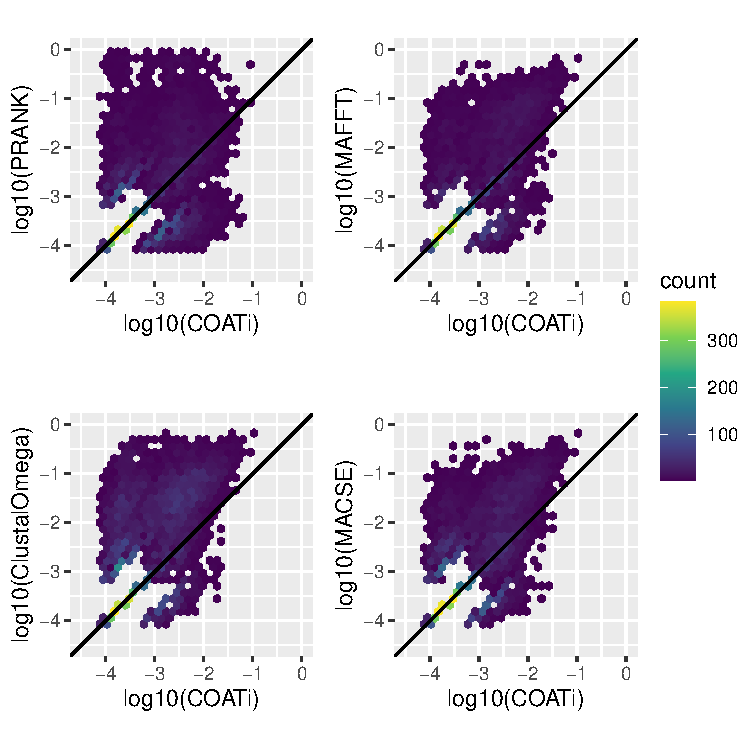
\includegraphics{chapter2/appendix-figures/dseq_plots_tri-mg.pdf}
    \caption[$d_{seq}$ Triplet-MG94]{Comparison of log10-transformed $d_{seq}$ data with pseudocounts between COATi codon-triplet-mg and PRANK, MAFFT, Clustal$\Omega$, and MACSE. COATi was significantly more accurate than other aligners; all p-values were $\leq 1.25e-76$.}
    \label{fig:dseq-tri-mg}
\end{figure}

\begin{figure}[!ht]
    \centering
    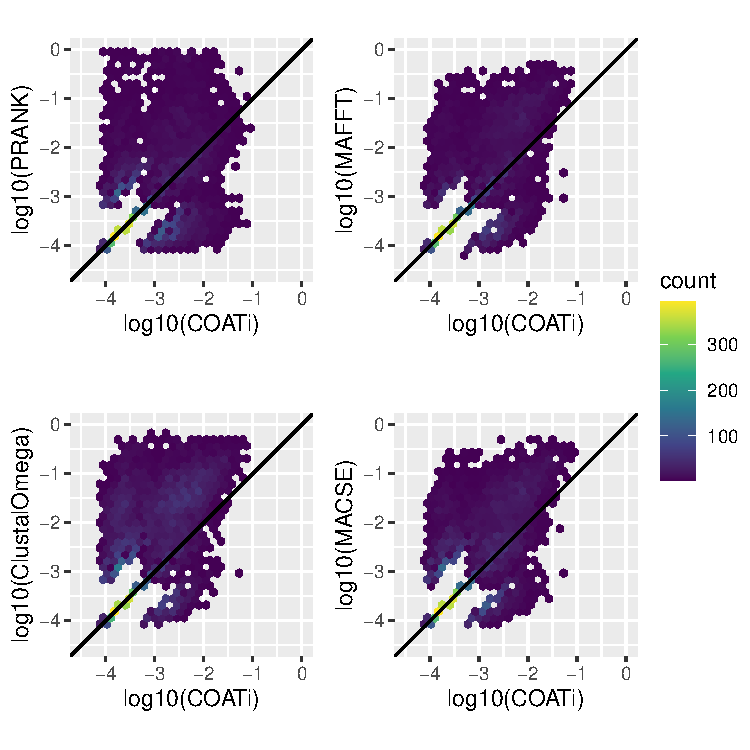
\includegraphics{chapter2/appendix-figures/dseq_plots_tri-ecm.pdf} 
    \caption[$d_{seq}$ Triplet-ECM]{Comparison of log10-transformed $d_{seq}$ data with pseudocounts between COATi codon-triplet-ecm and PRANK, MAFFT, Clustal$\Omega$, and MACSE. COATi was significantly more accurate than other aligners; all p-values were $\leq 3.23e-48$.}
    \label{fig:dseq-tri-ecm} 
\end{figure}

\begin{figure}[!ht]
    \centering
    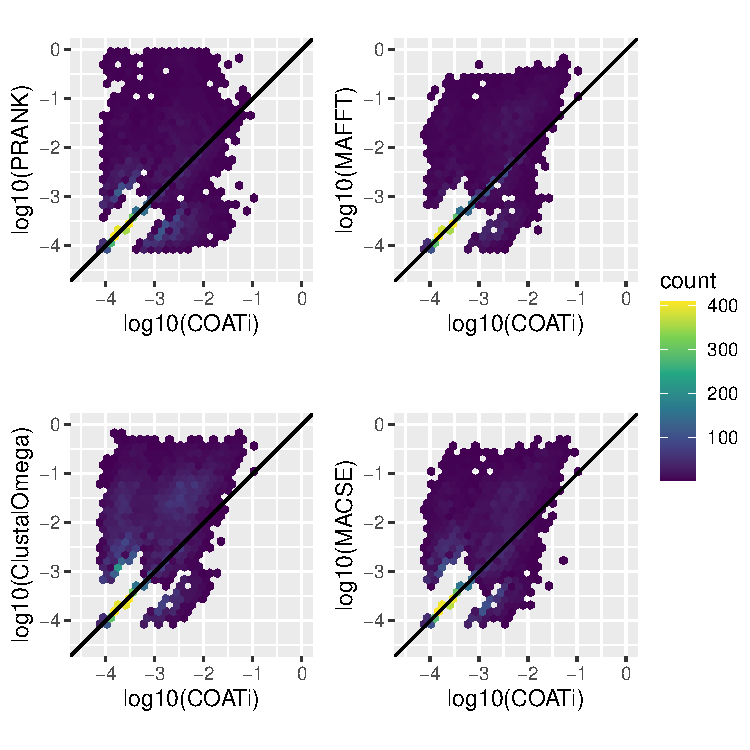
\includegraphics{chapter2/appendix-figures/dseq_plots_mar-mg.pdf} 
    \caption[$d_{seq}$ Marginal-MG94]{Comparison of log10-transformed $d_{seq}$ data with pseudocounts between COATi codon-marginal-mg and PRANK, MAFFT, Clustal$\Omega$, and MACSE. COATi was significantly more accurate than other aligners; all p-values were $\leq 1.99e-53$.}
    \label{fig:dseq-mar-mg}
\end{figure}

\begin{figure}![ht]
    \centering
    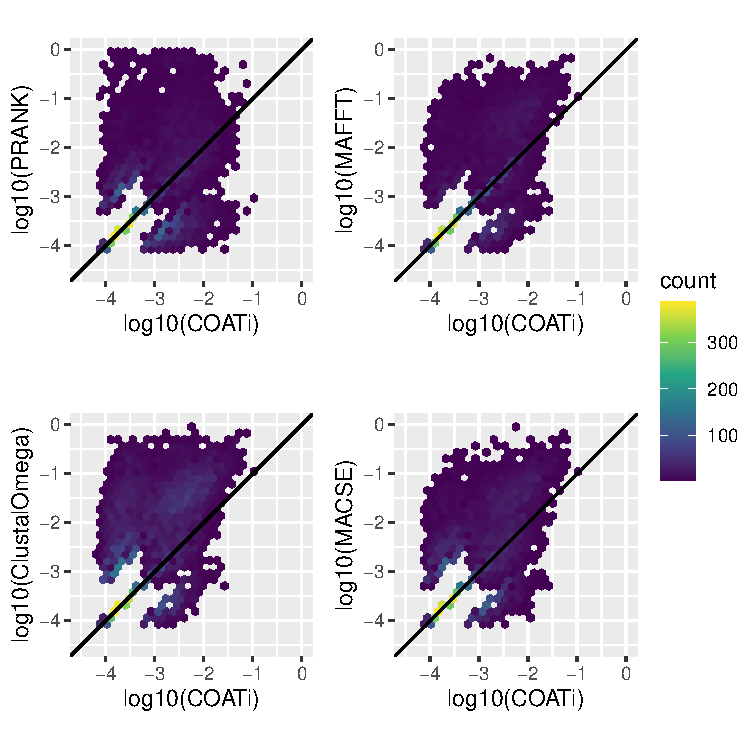
\includegraphics{chapter2/appendix-figures/dseq_plots_mar-ecm.pdf} 
    \caption[$d_{seq}$ Marginal-ECM]{Comparison of log10-transformed $d_{seq}$ data with pseudocounts between COATi codon-marginal-ecm and PRANK, MAFFT, Clustal$\Omega$, and MACSE. COATi was significantly more accurate than other aligners; all p-values were $\leq 1.44e-52$.}
    \label{fig:dseq-mar-ecm}
\end{figure}

\clearpage

% \section{Supplementary Methods} \label{supplementary-methods}

% Ks and Ka represent the number of substitutions per synonymous and
% non-synonymous sites. The ratio of nonsynonymous (Ka) to synonymous (Ks)
% nucleotide substitution rates indicates the selective pressures acting
% on genes. If the ratio is significantly greater than 1, it suggests
% positive selective pressure, meaning that nonsynonymous substitutions
% occur more frequently than synonymous substitutions. A ratio around 1
% can indicate either neutral evolution at the protein level or a mixture
% of positive and negative selective pressures. If the ratio is less than
% 1, it indicates a pressure to maintain protein sequence, known as
% purifying selection. Ks and Ka are calculated using the R package seqinr
% v.4.2-30 \citep{seqinr}.

 \newpage 
 \newpage \chapter{Supplementary Information for Chapter 3} \label{ch:ch3-supplement}

\section{Alignment Accuracy of the Triplet and Marginal ECM Models}

\begin{table}[!ht]
\centering

% matrix
\begingroup\centering
\begin{tabular}{r|ccccc}
      \textbf{t} & \textbf{Model} & \textbf{$d_{seq}$} & \textbf{Perfect alns} & \textbf{Imperfect alns}\\
\hline
\hline
0.2 & tri-ecm & 4.075938e-04 & 11609 & 538\\
0.2 & mar-ecm-sum & 2.254086e-03 & 9568 & 2578\\
0.2 & mar-ecm-max & 1.153611e-02 & 3955 & 7941\\
\hline
0.4 & tri-ecm & 5.674235e-04 & 11146 & 439\\
0.4 & mar-ecm-sum & 2.782803e-03 & 9271 & 2333\\
0.4 & mar-ecm-max & 0.0330844 & 1751 & 9599\\
\hline
0.6 & tri-ecm & 7.325429e-04 & 10681 & 377\\
0.6 & mar-ecm-sum & 3.134104e-03 & 9007 & 2020\\
0.6 & mar-ecm-max & 7.975872e-02 & 669 & 10130\\
\hline
0.8 & tri-ecm & 9.450685e-04 & 10354 & 388\\
0.8 & mar-ecm-sum & 3.621644e-03 & 8862 & 1854\\
0.8 & mar-ecm-max & 1.771613e-01 & 197 & 10322\\
\hline
1.0 & tri-ecm & 1.202495e-03 & 9999 & 361\\
1.0 & mar-ecm-sum & 4.194538e-03 & 8646 & 1720\\
1.0 & mar-ecm-max & 3.459159e-01 & 55 & 10155\\
\end{tabular}
\par\endgroup
% end matrix
 \caption[Alignment Accuracy of the Triplet and Marginal ECM Models]{Table with complete results comparing results of triplet-ecm, marginal-ecm-max, and marginal-ecm-sum COATi models in aligning 13,758 simulated sequence pairs. The triplet-ecm model generates better alignments across all branch lengths. Best alignments have the lowest $d_{seq}$, perfect alignments have the same score as the true alignment or a zero $d_{seq}$, and imperfect alignments have a different score than true alignments when at least one model found a perfect alignment.}
 \label{table:results-ecm}
\end{table}

\section{Benchmark Across Different CPUs}
\begin{figure}[!ht]
    \centering
    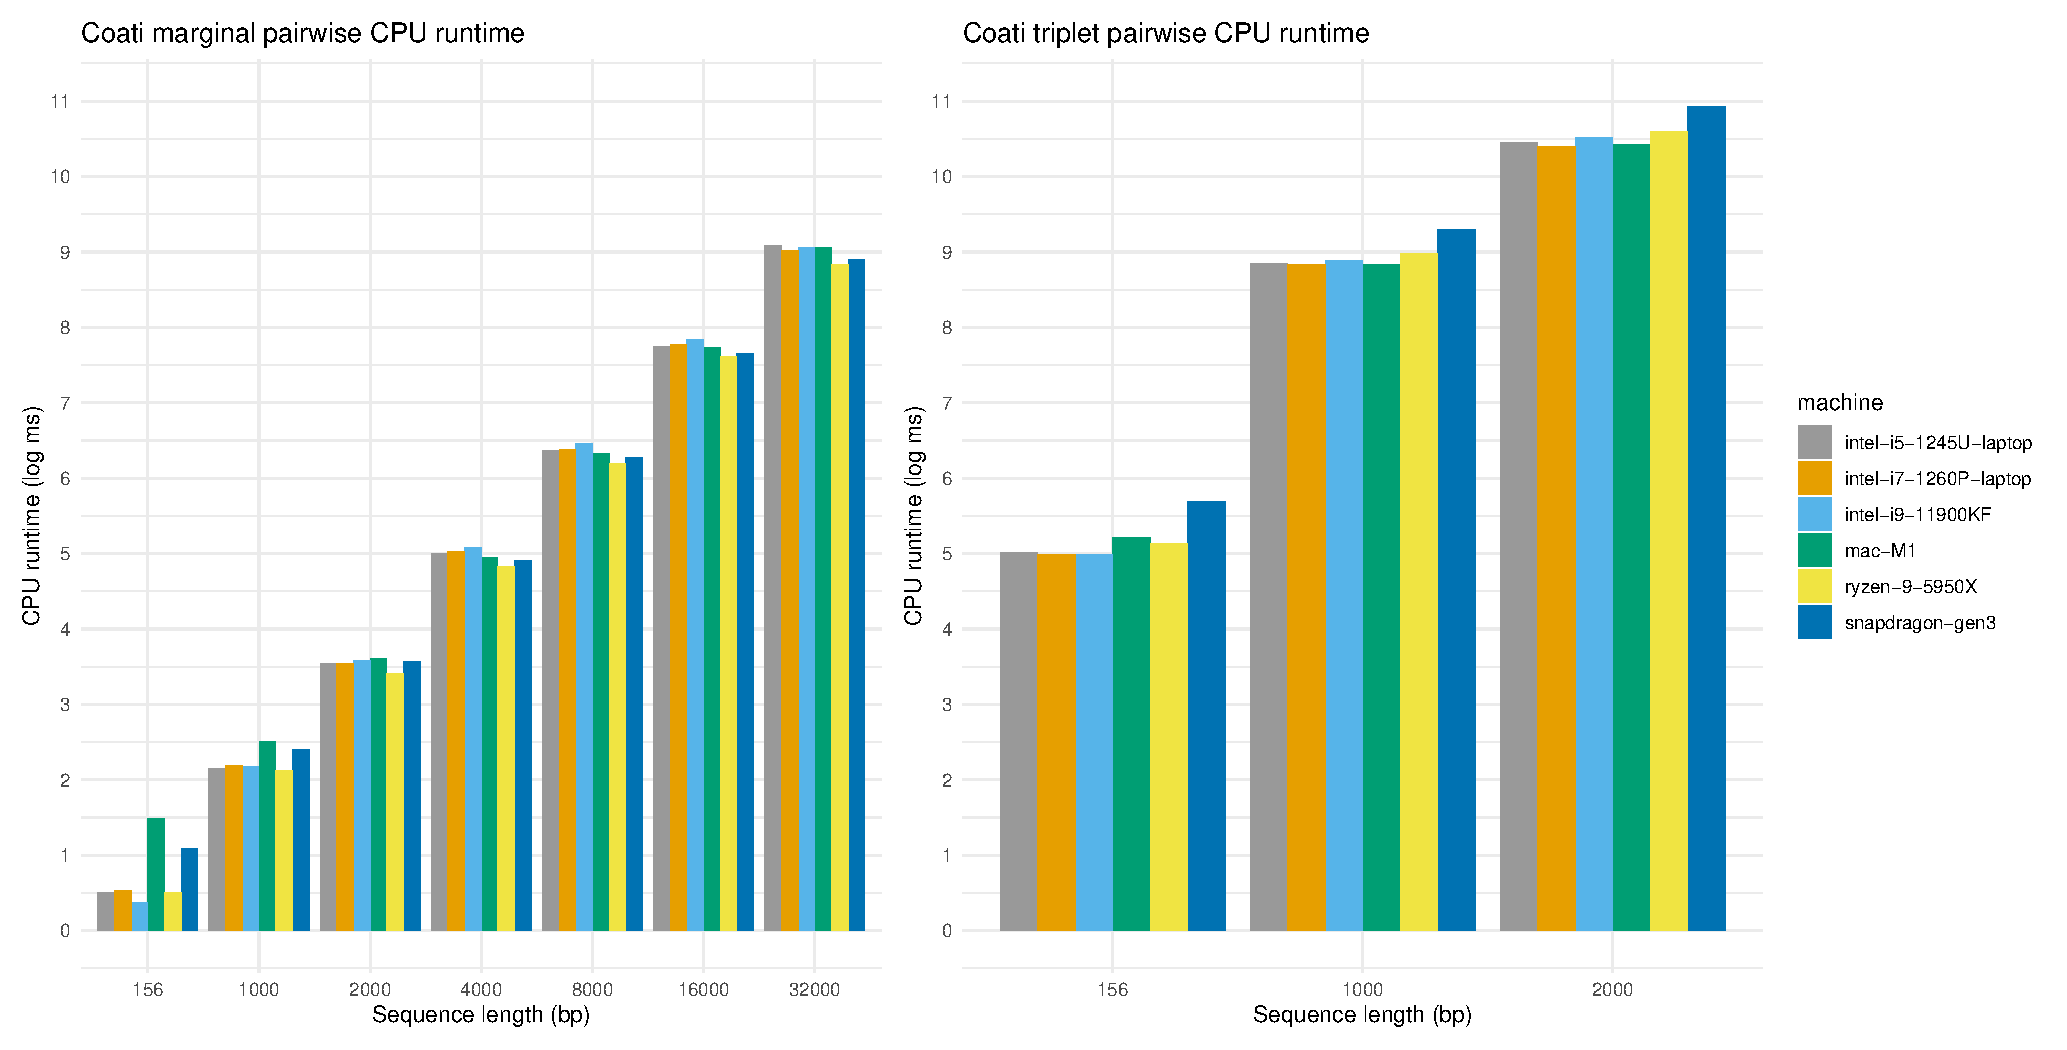
\includegraphics[width = \textwidth]{chapter3/figures/results/benchmarks.pdf}
    \caption[Runtime Comparison of Triplet and Marginal COATi Models]{Runtime benchmark of COATi marginal and triplet on different CPUs. Runtime is measured in seconds, while the benchmark consists of different length alignments.}
    \label{fig:cpu-runtime}
\end{figure}

% \section{coati-format}
% \section{coati-msa} \newpage 
% \include{vita}
\end{document}
